%%%%%%%%%%%%%%%%%%%%%%%%%%%%%%%%%%%%%%%%%
% The Legrand Orange Book
% LaTeX Template
% Version 2.0 (9/2/15)
%
% This template has been downloaded from:
% http://www.LaTeXTemplates.com
%
% Mathias Legrand (legrand.mathias@gmail.com) with modifications by:
% Vel (vel@latextemplates.com)
%
% License:
% CC BY-NC-SA 3.0 (http://creativecommons.org/licenses/by-nc-sa/3.0/)
%
% Compiling this template:
% This template uses biber for its bibliography and makeindex for its index.
% When you first open the template, compile it from the command line with the 
% commands below to make sure your LaTeX distribution is configured correctly:
%
% 1) pdflatex main
% 2) makeindex main.idx -s StyleInd.ist
% 3) biber main
% 4) pdflatex main x 2
%
% After this, when you wish to update the bibliography/index use the appropriate
% command above and make sure to compile with pdflatex several times 
% afterwards to propagate your changes to the document.
%
% This template also uses a number of packages which may need to be
% updated to the newest versions for the template to compile. It is strongly
% recommended you update your LaTeX distribution if you have any
% compilation errors.
%
% Important note:
% Chapter heading images should have a 2:1 width:height ratio,
% e.g. 920px width and 460px height.
%
%%%%%%%%%%%%%%%%%%%%%%%%%%%%%%%%%%%%%%%%%

%----------------------------------------------------------------------------------------
%	PACKAGES AND OTHER DOCUMENT CONFIGURATIONS
%----------------------------------------------------------------------------------------

\documentclass[14pt]{extbook} % Default font size and left-justified equations

\usepackage{float}% para ter [H]
\usepackage{fancyvrb}

%----------------------------------------------------------------------------------------
%	DATOS DEL LIBRO
%----------------------------------------------------------------------------------------
\newcommand{\mytitle}[0]{ Samba de Gafieira }
\newcommand{\mysubtitle}[0]{ Dan{\c{c}}a e Partitura de Movimento}
\newcommand{\myauthor}[0]{ Fernando Pujaico Rivera}
%----------------------------------------------------------------------------------------
\newcommand{\imprimirlocal}[0]{Brasil}
\newcommand{\imprimiryear}[0]{XXXXXXXXXXX}
\newcommand{\imprimirdata}[0]{9 de abril do \imprimiryear}
\newcommand{\imprimirtipotrabalho}[0]{Bibliografia}
\newcommand{\imprimirsize}[0]{16x30cm}
\newcommand{\imprimirisbn}[0]{XXXXXXXXXXX}
\newcommand{\imprimireditora}[0]{Editora XXXXXXXXXXX}
%----------------------------------------------------------------------------------------
\newcommand{\ImprimirLinkHomePageLivro}[0]{\url{http://XXXXXXXXXXX.com}}
\newcommand{\ImprimirLinkCompraLivroImpresso}[0]{\url{http://XXXXXXXXXXX.com/comprarfisico/}}
\newcommand{\ImprimirLinkCompraLivroDigital}[0]{\url{http://XXXXXXXXXXX.com/comprardigital/}}
%----------------------------------------------------------------------------------------
\newcommand{\ImprimirEmail}[0]{ \href{mailto:fernando.pujaico.rivera@gmail.com}{fernando.pujaico.rivera@gmail.com}}
%----------------------------------------------------------------------------------------

\newcommand{\AnoLivro}[0]{2019}%% Ano da primeira edição, usado para ser remplazado po ATUALMENTE

%----------------------------------------------------------------------------------------

\newcommand{\footwork}[0]{jogo de p\'{e}s}
\newcommand{\Footwork}[0]{Jogo de p\'{e}s}
\newcommand{\Variante}[0]{Variante}
\newcommand{\workboxsize}[0]{1.0\textwidth}
\newcommand{\bodycontrol}[0]{control corporal}
\newcommand{\Bodycontrol}[0]{Control corporal}
\newcommand{\bodyisolation}[0]{dissocia\c{c}\~{a}o corporal}
\newcommand{\Bodyisolation}[0]{Dissocia\c{c}\~{a}o corporal}
\newcommand{\bodyboxsize}[0]{0.75\textwidth}

%----------------------------------------------------------------------------------------
%	XCOLOR
%----------------------------------------------------------------------------------------
\usepackage[dvipsnames*,svgnames]{xcolor}
\definecolor{colorlowgray}{RGB}{240,240,240}
\definecolor{colorsystemdefault}{RGB}{16,81,15} % Define the color used for highlighting throughout the book
\definecolor{colorsystemdefaultdkred}{RGB}{98,32,6} % Define the color used for highlighting throughout the book
\definecolor{colormylink}{RGB}{16,120,15} % Define the 
\definecolor{dkred}{rgb}{0.6,0,0}


%\definecolor{fboxbackcolor}{RGB}{249,238,241}
%\definecolor{fboxfrontcolor}{RGB}{36,21,47}
\colorlet{fboxbackcolor}{colorsystemdefault!40!dkred}
\colorlet{fboxfrontcolor}{colorsystemdefault!40!dkred}

%----------------------------------------------------------------------------------------
%	COLOR
%----------------------------------------------------------------------------------------
\usepackage{color}
\definecolor{colorlowred}{rgb}{0.98,0.88,0.82}
%\definecolor{colordarkgray}{rgb}{0.5,0.5,0.5}
%\definecolor{colormauve}{rgb}{0.58,0,0.82}

%----------------------------------------------------------------------------------------


%----------------------------------------------------------------------------------------
%	VARIOUS REQUIRED PACKAGES AND CONFIGURATIONS
%----------------------------------------------------------------------------------------

\usepackage[top=3cm,bottom=3cm,left=3cm,right=3cm,headsep=10pt,a4paper]{geometry} % Page margins

\usepackage{graphicx} % Required for including pictures
\graphicspath{{pictures/}} % Specifies the directory where pictures are stored

\usepackage{lipsum} % Inserts dummy text

\usepackage[brazil]{babel}
%\usepackage[english]{babel} % English language/hyphenation

%----------------------------------------------------------------------------------------
%	Footnote
%----------------------------------------------------------------------------------------
\usepackage{scrextend} %multiple reference

%----------------------------------------------------------------------------------------
% Page counter
%----------------------------------------------------------------------------------------
\usepackage{lastpage}

%----------------------------------------------------------------------------------------
% GLOSSARIO
%----------------------------------------------------------------------------------------
\usepackage{nomencl}


%----------------------------------------------------------------------------------------
% Par diferentes modelos de caption.
%----------------------------------------------------------------------------------------
\usepackage{caption}
\usepackage{subcaption}
%\usepackage{wrapfig}

%----------------------------------------------------------------------------------------
% Para \singlespacing 
%----------------------------------------------------------------------------------------
\usepackage{setspace}

%----------------------------------------------------------------------------------------
% Para 
% \begin{inparaenum}
% \item
% \end{inparaenum}
% parecido a timeze pero horizontal 
%----------------------------------------------------------------------------------------

\usepackage{paralist}

%----------------------------------------------------------------------------------------
% MUSICAL NOTATION
%----------------------------------------------------------------------------------------
\usepackage[generate,ps2eps]{abc}%%sudo apt-get install abcm2ps
\usepackage[nointegrals]{wasysym}
\usepackage{harmony}


%----------------------------------------------------------------------------------------
% QR CODE
%----------------------------------------------------------------------------------------
%\usepackage{qrcode}

%----------------------------------------------------------------------------------------
%	BIBLIOGRAPHY AND INDEX
%----------------------------------------------------------------------------------------

\usepackage[ style=alphabetic,
             citestyle=alphabetic,
             sorting=none,
             sortcites=true,
             autopunct=true,
             babel=hyphen,
             hyperref=true,
             abbreviate=false,
             backref=true,
             backend=biber]{biblatex}
\addbibresource{bibliography/historiasamba.bib} % BibTeX bibliography file
\addbibresource{bibliography/historiabatuque.bib} % BibTeX bibliography file
\addbibresource{bibliography/historiamusicasamba.bib} % BibTeX bibliography file
\addbibresource{bibliography/historiagafieira.bib} % BibTeX bibliography file
\addbibresource{bibliography/musicateoria.bib} % BibTeX bibliography file
\addbibresource{bibliography/regras.bib} % BibTeX bibliography file
\addbibresource{bibliography/apendice-girias.bib} % BibTeX bibliography file
\defbibheading{bibempty}{}


\usepackage{calc} % For simpler calculation - used for spacing the index letter headings correctly
\usepackage{makeidx} % Required to make an index
\makeindex % Tells LaTeX to create the files required for indexing


 % paquetes usados con macros para la escrita
%%%%%%%%%%%%%%%%%%%%%%%%%%%%%%%%%%%%%%%%%
% The Legrand Orange Book
% Structural Definitions File
% Version 2.0 (9/2/15)
%
% Original author:
% Mathias Legrand (legrand.mathias@gmail.com) with modifications by:
% Vel (vel@latextemplates.com)
% 
% This file has been downloaded from:
% http://www.LaTeXTemplates.com
%
% License:
% CC BY-NC-SA 3.0 (http://creativecommons.org/licenses/by-nc-sa/3.0/)
%
%%%%%%%%%%%%%%%%%%%%%%%%%%%%%%%%%%%%%%%%%

%----------------------------------------------------------------------------------------
%	VARIOUS REQUIRED PACKAGES AND CONFIGURATIONS
%----------------------------------------------------------------------------------------


\usepackage{tikz} % Required for drawing custom shapes


\usepackage{enumitem} % Customize lists
\setlist{nolistsep} % Reduce spacing between bullet points and numbered lists

\usepackage{booktabs} % Required for nicer horizontal rules in tables




%----------------------------------------------------------------------------------------
%	FONTS
%----------------------------------------------------------------------------------------

\usepackage{avant} % Use the Avantgarde font for headings
%\usepackage{times} % Use the Times font for headings
\usepackage{mathptmx} % Use the Adobe Times Roman as the default text font together with math symbols from the Sym­bol, Chancery and Com­puter Modern fonts

\usepackage{microtype} % Slightly tweak font spacing for aesthetics
\usepackage[utf8]{inputenc} % Required for including letters with accents
\usepackage[T1]{fontenc} % Use 8-bit encoding that has 256 glyphs



%----------------------------------------------------------------------------------------
%	MAIN TABLE OF CONTENTS
%----------------------------------------------------------------------------------------

\usepackage{titletoc} % Required for manipulating the table of contents

\contentsmargin{0cm} % Removes the default margin

% Part text styling
\titlecontents{part}[0cm]
{\addvspace{20pt}\centering\large\bfseries}
{}
{}
{}

% Chapter text styling
\titlecontents{chapter}[1.25cm] % Indentation
{\addvspace{12pt}\large\sffamily\bfseries} % Spacing and font options for chapters
{\color{ocre!60}\contentslabel[\Large\thecontentslabel]{1.25cm}\color{ocre}} % Chapter number
{\color{ocre}}  
{\color{ocre!60}\normalsize\;\titlerule*[.5pc]{.}\;\thecontentspage} % Page number

% Section text styling
\titlecontents{section}[2.00cm] % Indentation
{\addvspace{3pt}\sffamily\bfseries} % Spacing and font options for sections
{\contentslabel[\thecontentslabel]{1.25cm}} % Section number
{}
{\hfill\color{black}\thecontentspage} % Page number
[]

% Subsection text styling
\titlecontents{subsection}[2.00cm] % Indentation
{\addvspace{1pt}\sffamily\small} % Spacing and font options for subsections
{\contentslabel[\thecontentslabel]{1.25cm}} % Subsection number
{}
{\ \titlerule*[.5pc]{.}\;\thecontentspage} % Page number
[]

% List of figures
\titlecontents{figure}[0em]
{\addvspace{-5pt}\sffamily}
{\thecontentslabel\hspace*{1em}}
{}
{\ \titlerule*[.5pc]{.}\;\thecontentspage}
[]

% List of tables
\titlecontents{table}[0em]
{\addvspace{-5pt}\sffamily}
{\thecontentslabel\hspace*{1em}}
{}
{\ \titlerule*[.5pc]{.}\;\thecontentspage}
[]

%----------------------------------------------------------------------------------------
%	MINI TABLE OF CONTENTS IN PART HEADS
%----------------------------------------------------------------------------------------

% Chapter text styling
\titlecontents{lchapter}[0em] % Indenting
{\addvspace{15pt}\large\sffamily\bfseries} % Spacing and font options for chapters
{\color{ocre}\contentslabel[\Large\thecontentslabel]{1.25cm}\color{ocre}} % Chapter number
{}  
{\color{ocre}\normalsize\sffamily\bfseries\;\titlerule*[.5pc]{.}\;\thecontentspage} % Page number

% Section text styling
\titlecontents{lsection}[0em] % Indenting
{\sffamily\small} % Spacing and font options for sections
{\contentslabel[\thecontentslabel]{1.25cm}} % Section number
{}
{}

% Subsection text styling
\titlecontents{lsubsection}[.5em] % Indentation
{\normalfont\footnotesize\sffamily} % Font settings
{}
{}
{}

%----------------------------------------------------------------------------------------
%	PAGE HEADERS
%----------------------------------------------------------------------------------------

\usepackage{fancyhdr} % Required for header and footer configuration

\pagestyle{fancy}
\renewcommand{\chaptermark}[1]{\markboth{\sffamily\normalsize\bfseries\chaptername\ \thechapter.\ #1}{}} % Chapter text font settings
\renewcommand{\sectionmark}[1]{\markright{\sffamily\normalsize\thesection\hspace{5pt}#1}{}} % Section text font settings
\fancyhf{} \fancyhead[LE,RO]{\sffamily\normalsize\thepage} % Font setting for the page number in the header
\fancyhead[LO]{\rightmark} % Print the nearest section name on the left side of odd pages
\fancyhead[RE]{\leftmark} % Print the current chapter name on the right side of even pages
\renewcommand{\headrulewidth}{0.5pt} % Width of the rule under the header
\addtolength{\headheight}{2.5pt} % Increase the spacing around the header slightly
\renewcommand{\footrulewidth}{0pt} % Removes the rule in the footer
\fancypagestyle{plain}{\fancyhead{}\renewcommand{\headrulewidth}{0pt}} % Style for when a plain pagestyle is specified

% Removes the header from odd empty pages at the end of chapters
\makeatletter
\renewcommand{\cleardoublepage}{
\clearpage\ifodd\c@page\else
\hbox{}
\vspace*{\fill}
\thispagestyle{empty}
\newpage
\fi}

%----------------------------------------------------------------------------------------
%	DEFINITION OF THEOREM BOXES
%----------------------------------------------------------------------------------------
\usepackage{amsmath,amsfonts,amssymb,amsthm} % For math equations, theorems, symbols, etc

\newcommand{\intoo}[2]{\mathopen{]}#1\,;#2\mathclose{[}}
\newcommand{\ud}{\mathop{\mathrm{{}d}}\mathopen{}}
\newcommand{\intff}[2]{\mathopen{[}#1\,;#2\mathclose{]}}
\newtheorem{notation}{Notation}[chapter]

% Boxed/framed environments
\newtheoremstyle{ocrenumbox}% % Theorem style name
{0pt}% Space above
{0pt}% Space below
{\normalfont}% % Body font
{}% Indent amount
{\small\bf\sffamily\color{ocre}}% % Theorem head font
{\;}% Punctuation after theorem head
{0.25em}% Space after theorem head
{\small\sffamily\color{ocre}\thmname{#1}\nobreakspace\thmnumber{\@ifnotempty{#1}{}\@upn{#2}}% Theorem text (e.g. Theorem 2.1)
\thmnote{\nobreakspace\the\thm@notefont\sffamily\bfseries\color{black}---\nobreakspace#3}} % Optional theorem note
\renewcommand{\qedsymbol}{$\blacksquare$}% Optional qed square

\newtheoremstyle{blacknumex}% Theorem style name
{5pt}% Space above
{5pt}% Space below
{\normalfont}% Body font
{} % Indent amount
{\small\bf\sffamily}% Theorem head font
{\;}% Punctuation after theorem head
{0.25em}% Space after theorem head
{\small\sffamily{\tiny\ensuremath{\blacksquare}}\nobreakspace\thmname{#1}\nobreakspace\thmnumber{\@ifnotempty{#1}{}\@upn{#2}}% Theorem text (e.g. Theorem 2.1)
\thmnote{\nobreakspace\the\thm@notefont\sffamily\bfseries---\nobreakspace#3}}% Optional theorem note

\newtheoremstyle{blacknumbox} % Theorem style name
{0pt}% Space above
{0pt}% Space below
{\normalfont}% Body font
{}% Indent amount
{\small\bf\sffamily}% Theorem head font
{\;}% Punctuation after theorem head
{0.25em}% Space after theorem head
{\small\sffamily\thmname{#1}\nobreakspace\thmnumber{\@ifnotempty{#1}{}\@upn{#2}}% Theorem text (e.g. Theorem 2.1)
\thmnote{\nobreakspace\the\thm@notefont\sffamily\bfseries---\nobreakspace#3}}% Optional theorem note

% Non-boxed/non-framed environments
\newtheoremstyle{ocrenum}% % Theorem style name
{5pt}% Space above
{5pt}% Space below
{\normalfont}% % Body font
{}% Indent amount
{\small\bf\sffamily\color{ocre}}% % Theorem head font
{\;}% Punctuation after theorem head
{0.25em}% Space after theorem head
{\small\sffamily\color{ocre}\thmname{#1}\nobreakspace\thmnumber{\@ifnotempty{#1}{}\@upn{#2}}% Theorem text (e.g. Theorem 2.1)
\thmnote{\nobreakspace\the\thm@notefont\sffamily\bfseries\color{black}---\nobreakspace#3}} % Optional theorem note
\renewcommand{\qedsymbol}{$\blacksquare$}% Optional qed square
\makeatother

% Defines the theorem text style for each type of theorem to one of the three styles above
\newcounter{dummy} 
\numberwithin{dummy}{section}
\theoremstyle{ocrenumbox}
\newtheorem{theoremeT}[dummy]{Theorem}
\newtheorem{problem}{Problem}[chapter]
\newtheorem{exerciseT}{Exercise}[chapter]
\theoremstyle{blacknumex}
\newtheorem{exampleT}{Exemplo}[chapter]
\theoremstyle{blacknumbox}
\newtheorem{vocabulary}{Vocabulary}[chapter]
\newtheorem{definitionT}{Definição}[chapter]
\newtheorem{corollaryT}[dummy]{Corollary}
\theoremstyle{ocrenum}
\newtheorem{proposition}[dummy]{Proposition}

%----------------------------------------------------------------------------------------
%	DEFINITION OF COLORED THEOREM BOXES
%----------------------------------------------------------------------------------------

\RequirePackage[framemethod=default]{mdframed} % Required for creating the theorem, definition, exercise and corollary boxes

% Theorem box
\newmdenv[skipabove=7pt,
skipbelow=7pt,
backgroundcolor=black!5,
linecolor=ocre,
innerleftmargin=5pt,
innerrightmargin=5pt,
innertopmargin=5pt,
leftmargin=0cm,
rightmargin=0cm,
innerbottommargin=5pt]{tBox}

% Exercise box	  
\newmdenv[skipabove=7pt,
skipbelow=7pt,
rightline=false,
leftline=true,
topline=false,
bottomline=false,
backgroundcolor=ocre!10,
linecolor=ocre,
innerleftmargin=5pt,
innerrightmargin=5pt,
innertopmargin=5pt,
innerbottommargin=5pt,
leftmargin=0cm,
rightmargin=0cm,
linewidth=4pt]{eBox}	

% Definition box
\newmdenv[skipabove=7pt,
skipbelow=7pt,
rightline=false,
leftline=true,
topline=false,
bottomline=false,
linecolor=ocre,
innerleftmargin=5pt,
innerrightmargin=5pt,
innertopmargin=0pt,
leftmargin=0cm,
rightmargin=0cm,
linewidth=4pt,
innerbottommargin=0pt]{dBox}	

% Corollary box
\newmdenv[skipabove=7pt,
skipbelow=7pt,
rightline=false,
leftline=true,
topline=false,
bottomline=false,
linecolor=gray,
backgroundcolor=black!5,
innerleftmargin=5pt,
innerrightmargin=5pt,
innertopmargin=5pt,
leftmargin=0cm,
rightmargin=0cm,
linewidth=4pt,
innerbottommargin=5pt]{cBox}

% Creates an environment for each type of theorem and assigns it a theorem text style from the "Theorem Styles" section above and a colored box from above
\newenvironment{theorem}{\begin{tBox}\begin{theoremeT}}{\end{theoremeT}\end{tBox}}
\newenvironment{exercise}{\begin{eBox}\begin{exerciseT}}{\hfill{\color{ocre}\tiny\ensuremath{\blacksquare}}\end{exerciseT}\end{eBox}}				  
\newenvironment{definition}{\begin{dBox}\begin{definitionT}}{\end{definitionT}\end{dBox}}	
\newenvironment{example}{\begin{exampleT}}{\hfill{\tiny\ensuremath{\blacksquare}}\end{exampleT}}		
\newenvironment{corollary}{\begin{cBox}\begin{corollaryT}}{\end{corollaryT}\end{cBox}}	

%----------------------------------------------------------------------------------------
%	REMARK ENVIRONMENT
%----------------------------------------------------------------------------------------
\newenvironment{remark}{\par\vspace{10pt}\small % Vertical white space above the remark and smaller font size
\begin{list}{}{
\leftmargin=35pt % Indentation on the left
\rightmargin=25pt}\item\ignorespaces % Indentation on the right
\makebox[-2.5pt]{\begin{tikzpicture}[overlay]
\node[draw=ocre!60,line width=1pt,circle,fill=ocre!25,font=\sffamily\bfseries,inner sep=2pt,outer sep=0pt] at (-15pt,0pt){\textcolor{ocre}{R}};\end{tikzpicture}} % Orange R in a circle
\advance\baselineskip -1pt}{\end{list}\vskip5pt} % Tighter line spacing and white space after remark

%----------------------------------------------------------------------------------------
%	SECTION NUMBERING IN THE MARGIN
%----------------------------------------------------------------------------------------
\makeatletter
\renewcommand{\@seccntformat}[1]{\llap{\textcolor{ocre}{\csname the#1\endcsname}\hspace{1em}}}                    
\renewcommand{\section}{\@startsection{section}{1}{\z@}
{-4ex \@plus -1ex \@minus -.4ex}
{1ex \@plus.2ex }
{\normalfont\large\sffamily\bfseries}}
\renewcommand{\subsection}{\@startsection {subsection}{2}{\z@}
{-3ex \@plus -0.1ex \@minus -.4ex}
{0.5ex \@plus.2ex }
{\normalfont\sffamily\bfseries}}
\renewcommand{\subsubsection}{\@startsection {subsubsection}{3}{\z@}
{-2ex \@plus -0.1ex \@minus -.2ex}
{.2ex \@plus.2ex }
{\normalfont\small\sffamily\bfseries}}                        
\renewcommand\paragraph{\@startsection{paragraph}{4}{\z@}
{-2ex \@plus-.2ex \@minus .2ex}
{.1ex}
{\normalfont\small\sffamily\bfseries}}

%----------------------------------------------------------------------------------------
%	PART HEADINGS
%----------------------------------------------------------------------------------------

% numbered part in the table of contents
\newcommand{\@mypartnumtocformat}[2]{%
\setlength\fboxsep{0pt}%
\noindent\colorbox{ocre!20}{\strut\parbox[c][.7cm]{\ecart}{\color{ocre!70}\Large\sffamily\bfseries\centering#1}}\hskip\esp\colorbox{ocre!40}{\strut\parbox[c][.7cm]{\linewidth-\ecart-\esp}{\Large\sffamily\centering#2}}}%
%%%%%%%%%%%%%%%%%%%%%%%%%%%%%%%%%%
% unnumbered part in the table of contents
\newcommand{\@myparttocformat}[1]{%
\setlength\fboxsep{0pt}%
\noindent\colorbox{ocre!40}{\strut\parbox[c][.7cm]{\linewidth}{\Large\sffamily\centering#1}}}%
%%%%%%%%%%%%%%%%%%%%%%%%%%%%%%%%%%
\newlength\esp
\setlength\esp{4pt}
\newlength\ecart
\setlength\ecart{1.2cm-\esp}
\newcommand{\thepartimage}{}%
\newcommand{\partimage}[1]{\renewcommand{\thepartimage}{#1}}%
\def\@part[#1]#2{%
\ifnum \c@secnumdepth >-2\relax%
\refstepcounter{part}%
\addcontentsline{toc}{part}{\texorpdfstring{\protect\@mypartnumtocformat{\thepart}{#1}}{\partname~\thepart\ ---\ #1}}
\else%
\addcontentsline{toc}{part}{\texorpdfstring{\protect\@myparttocformat{#1}}{#1}}%
\fi%
\startcontents%
\markboth{}{}%
{\thispagestyle{empty}%
\begin{tikzpicture}[remember picture,overlay]%
\node at (current page.north west){\begin{tikzpicture}[remember picture,overlay]%	
\fill[ocre!20](0cm,0cm) rectangle (\paperwidth,-\paperheight);
\node[anchor=north] at (4cm,-3.25cm){\color{ocre!40}\fontsize{220}{100}\sffamily\bfseries\@Roman\c@part}; 
\node[anchor=south east] at (\paperwidth-1cm,-\paperheight+1cm){\parbox[t][][t]{8.5cm}{
\printcontents{l}{0}{\setcounter{tocdepth}{1}}%
}};
\node[anchor=north east] at (\paperwidth-1.5cm,-3.25cm){\parbox[t][][t]{15cm}{\strut\raggedleft\color{white}\fontsize{30}{30}\sffamily\bfseries#2}};
\end{tikzpicture}};
\end{tikzpicture}}%
\@endpart}
\def\@spart#1{%
\startcontents%
\phantomsection
{\thispagestyle{empty}%
\begin{tikzpicture}[remember picture,overlay]%
\node at (current page.north west){\begin{tikzpicture}[remember picture,overlay]%	
\fill[ocre!20](0cm,0cm) rectangle (\paperwidth,-\paperheight);
\node[anchor=north east] at (\paperwidth-1.5cm,-3.25cm){\parbox[t][][t]{15cm}{\strut\raggedleft\color{white}\fontsize{30}{30}\sffamily\bfseries#1}};
\end{tikzpicture}};
\end{tikzpicture}}
\addcontentsline{toc}{part}{\texorpdfstring{%
\setlength\fboxsep{0pt}%
\noindent\protect\colorbox{ocre!40}{\strut\protect\parbox[c][.7cm]{\linewidth}{\Large\sffamily\protect\centering #1\quad\mbox{}}}}{#1}}%
\@endpart}
\def\@endpart{\vfil\newpage
\if@twoside
\if@openright
\null
\thispagestyle{empty}%
\newpage
\fi
\fi
\if@tempswa
\twocolumn
\fi}

%----------------------------------------------------------------------------------------
%	CHAPTER HEADINGS
%----------------------------------------------------------------------------------------
\newcommand{\thechapterimage}{}%
\newcommand{\chapterimage}[1]{\renewcommand{\thechapterimage}{#1}}%
\def\@makechapterhead#1{%
{\parindent \z@ \raggedright \normalfont
\ifnum \c@secnumdepth >\m@ne
\if@mainmatter
\begin{tikzpicture}[remember picture,overlay]
\node at (current page.north west)
{\begin{tikzpicture}[remember picture,overlay]
\node[anchor=north west,inner sep=0pt] at (0,0) {\includegraphics[width=\paperwidth]{\thechapterimage}};
\draw[anchor=west] (\Gm@lmargin,-9cm) node [line width=2pt,rounded corners=15pt,draw=ocre,fill=white,fill opacity=0.5,inner sep=15pt]{\strut\makebox[22cm]{}};
\draw[anchor=west] (\Gm@lmargin+.3cm,-9cm) node {\huge\sffamily\bfseries\color{black}\thechapter. #1\strut};
\end{tikzpicture}};
\end{tikzpicture}
\else
\begin{tikzpicture}[remember picture,overlay]
\node at (current page.north west)
{\begin{tikzpicture}[remember picture,overlay]
\node[anchor=north west,inner sep=0pt] at (0,0) {\includegraphics[width=\paperwidth]{\thechapterimage}};
\draw[anchor=west] (\Gm@lmargin,-9cm) node [line width=2pt,rounded corners=15pt,draw=ocre,fill=white,fill opacity=0.5,inner sep=15pt]{\strut\makebox[22cm]{}};
\draw[anchor=west] (\Gm@lmargin+.3cm,-9cm) node {\huge\sffamily\bfseries\color{black}#1\strut};
\end{tikzpicture}};
\end{tikzpicture}
\fi\fi\par\vspace*{270\p@}}}

%-------------------------------------------

\def\@makeschapterhead#1{%
\begin{tikzpicture}[remember picture,overlay]
\node at (current page.north west)
{\begin{tikzpicture}[remember picture,overlay]
\node[anchor=north west,inner sep=0pt] at (0,0) {\includegraphics[width=\paperwidth]{\thechapterimage}};
\draw[anchor=west] (\Gm@lmargin,-9cm) node [line width=2pt,rounded corners=15pt,draw=ocre,fill=white,fill opacity=0.5,inner sep=15pt]{\strut\makebox[22cm]{}};
\draw[anchor=west] (\Gm@lmargin+.3cm,-9cm) node {\huge\sffamily\bfseries\color{black}#1\strut};
\end{tikzpicture}};
\end{tikzpicture}
\par\vspace*{270\p@}}
\makeatother

%----------------------------------------------------------------------------------------
%	HYPERLINKS IN THE DOCUMENTS
%----------------------------------------------------------------------------------------
\usepackage{hyperref}
\hypersetup{
	hidelinks,
	backref=true,
	pagebackref=true,
	hyperindex=true,
	colorlinks=true,
	linkcolor=black,         % color of internal links (change box color with linkbordercolor)
	%pdftoolbar=true,         % show Acrobat’s toolbar?
	%pdfmenubar=true,         % show Acrobat’s menu?
	%pdffitwindow=false,      % window fit to page when opened
	%pdfstartview={FitH},     % fits the width of the page to the window
	breaklinks=true,
	urlcolor= colormylink,
	bookmarks=true,
	bookmarksopen=false,
	pdftitle={Title},
	pdfauthor={Author}
}

\usepackage{bookmark}
\bookmarksetup{
open,
numbered,
addtohook={%
\ifnum\bookmarkget{level}=0 % chapter
\bookmarksetup{bold}%
\fi
\ifnum\bookmarkget{level}=-1 % part
\bookmarksetup{color=colormylink,bold}%
\fi
}
}
 % el estilo visual do livro

\usepackage{morewrites}%%! No room for a new \write.


%----------------------------------------------------------------------------------------
%  footnote font size
%----------------------------------------------------------------------------------------
\renewcommand{\footnotesize}{\small}

%----------------------------------------------------------------------------------------
%	Horizontal separator line
%   \HRule{2pt}
%----------------------------------------------------------------------------------------
\newcommand{\HRule}[1]{\rule{\linewidth}{#1}} % creo el comando  \HRule regla horizontal



%----------------------------------------------------------------------------------------
%	Horizontal separator line
%   \PRLsep{Text}
%----------------------------------------------------------------------------------------
\newlength{\PRLlen}
\newcommand*\PRLsep[1]{\settowidth{\PRLlen}{#1}\advance\PRLlen by -\textwidth\divide\PRLlen by -2\noindent\makebox[\the\PRLlen]{\resizebox{\the\PRLlen}{1pt}{$\blacktriangleleft$}}\raisebox{-.5ex}{\textbf{#1}}\makebox[\the\PRLlen]{\resizebox{\the\PRLlen}{1pt}{$\blacktriangleright$}}\smallskip}


%----------------------------------------------------------------------------------------
%----------------------------------------------------------------------------------------
%----------------------------------------------------------------------------------------
%----------------------------------------------------------------------------------------
% BOX - TCOLORBOX
%----------------------------------------------------------------------------------------
\usepackage[most,many]{tcolorbox}
\usetikzlibrary{decorations.pathmorphing}
\tcbuselibrary{skins}
%----------------------------------------------------------------------------------------
% ATTENTION MESSAGE BOX
%----------------------------------------------------------------------------------------
% \begin{tcbattention}
%   text
% \end{tcbattention}

\newtcolorbox{tcbattention}[1][]{enhanced,
  before skip=2mm,after skip=3mm,
  boxrule=0.4pt,left=5mm,right=2mm,top=1mm,bottom=1mm,
  colback=colorAttention!50,
  colframe=colorAttention!20!black,
  sharp corners,rounded corners=southeast,arc is angular,arc=3mm,
  underlay={%
    \path[fill=colorsystemdefault!20!black] ([yshift=3mm]interior.south east)--++(-0.4,-0.1)--++(0.1,-0.2);
    \path[draw=colorsystemdefault,shorten <=-0.05mm,shorten >=-0.05mm] ([yshift=3mm]interior.south east)--++(-0.4,-0.1)--++(0.1,-0.2);
    \path[fill=colorAttention!50!black,draw=none] (interior.south west) rectangle node[white]{\Huge\bfseries !} ([xshift=4mm]interior.north west);
    },
  drop fuzzy shadow,#1}
  
%----------------------------------------------------------------------------------------
% DEFINITION THEOREMS
%----------------------------------------------------------------------------------------
% \begin{definition}[Título]
%   text
% \end{definition}
%----------------------------------------------------------------------------------------
%% Create a new counter that will follow tcolorbox's numbering
\newcounter{definition}[section]
\renewcommand*{\thedefinition}{\noexpand\thesection.\noexpand\arabic{definition}}

\newtcolorbox[list inside=MisDefinicoes,list type=MisDefinicoes,auto counter,number within=section]{definition}[1][]{
  title={#1},
  detach title,
  coltitle=black,
  before upper={\addtocounter{definition}{-1}\refstepcounter{definition}\textbf{Defini\c{c}\~{a}o~\thetcbcounter\refstepcounter{definition}\ifdefstring{\tcbtitletext}{}{:}{~---~\tcbtitle:}}},
  % %fonttitle=\bfseries,
  breakable,
  enhanced,
  arc      =0mm,
  top=0mm,
  bottom=0mm,
  colback  =black!3,
  colframe =colorsystemdefault,
  leftrule =4pt,%
  rightrule=0mm,
  toprule=0mm,
  bottomrule=0mm,
  %drop fuzzy shadow=black
}


%% List of type %% para:  \tcblistof[\section*]{MisDefinicoes}{Lista de frases}
\titlecontents{MisDefinicoes}[2.00cm] %% Indentation %% left
{\addvspace{3pt}\sffamily\bfseries} %% Spacing and font options for sections %% above code
{\contentslabel[{\thecontentslabel}]{1.45cm}} %% Section number %% numbered-entry-format % {\thetcbcounter}%
{} %% numberless-entry-format
{\ \titlerule*[.5pc]{.}\;\color{black}\thecontentspage} %% filler-page-format {\hfill\color{black}\thecontentspage} 
[] %% separator

\makeatletter
\newcommand{\ttll@MisDefinicoes}{-1000}
\makeatother


%----------------------------------------------------------------------------------------
% INFORMATION MESSAGE BOX
%----------------------------------------------------------------------------------------
% \begin{tcbinformation}{Título}
%   text
% \end{tcbinformation}
%----------------------------------------------------------------------------------------
\newtcolorbox[list inside=MisInformacoes,list type=MisInformacoes,auto counter,number within=chapter]{tcbinformation}[1]
{
  title={#1},
  detach title,
  coltitle=black,
  before upper={\textbf{\tcbtitle: }},
  % %fonttitle=\bfseries,
  breakable,
  enhanced,
  arc      =2mm,
  colback  =colorsystemdefault!5,
  colframe =colorsystemdefault,
  leftrule =14mm,%
  drop fuzzy shadow=black,
  overlay  ={\node[anchor=north west,outer sep=4pt] at (frame.north west) {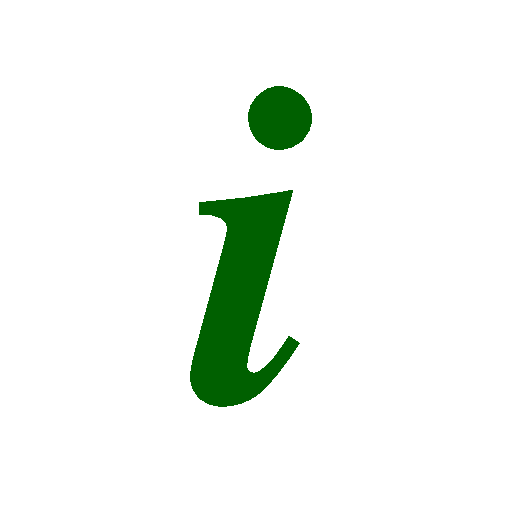
\includegraphics[width=8mm]{information1.eps}}; }
}


%% List of type %% para:  \tcblistof[\section*]{MisInformacoes}{Lista de frases}
\titlecontents{MisInformacoes}[2.00cm] %% Indentation %% left
{\addvspace{3pt}\sffamily\bfseries} %% Spacing and font options for sections %% above code
{\contentslabel[{\thecontentslabel}]{1.45cm}} %% Section number %% numbered-entry-format % {\thetcbcounter}%
{} %% numberless-entry-format
{\ \titlerule*[.5pc]{.}\;\color{black}\thecontentspage} %% filler-page-format {\hfill\color{black}\thecontentspage} 
[] %% separator

\makeatletter
\newcommand{\ttll@MisInformacoes}{-1000}
\makeatother

%----------------------------------------------------------------------------------------
% ELABORACION MESSAGE BOX
%----------------------------------------------------------------------------------------
% \begin{elaboracion}{título}
%   texto
% \end{elaboracion}
%\newcounter{countelab}%[chapter] ,use counter=countelab
\newtcolorbox[list inside=MisElaboraciones,list type=MisElaboraciones,auto counter,number within=chapter]{elaboracion}[1]{
    tile,
    colback=colorsystemdefaultdkred!3,
    coltitle=white,
    colbacktitle=colorsystemdefaultdkred,
    center title,
    toprule=1.25mm,
    bottomrule=1.25mm,
    extras unbroken and first={borderline north={0.5mm}{0.5mm}{colorsystemdefaultdkred,decoration={zigzag,amplitude=0.5mm},decorate}},
    extras unbroken and last={borderline south={0.5mm}{0.5mm}{colorsystemdefaultdkred,decoration={zigzag,amplitude=0.5mm},decorate}},
    title={#1}, 
    width=\linewidth
}



%% List of type %% para:  \tcblistof[\section*]{MisXElaboraciones}{Lista de frases}
\titlecontents{MisElaboraciones}[2.00cm] %% Indentation %% left
{\addvspace{3pt}\sffamily\bfseries} %% Spacing and font options for sections %% above code
{\contentslabel[{\thecontentslabel}]{1.45cm}} %% Section number %% numbered-entry-format % {\thetcbcounter}%
{} %% numberless-entry-format
{\ \titlerule*[.5pc]{.}\;\color{black}\thecontentspage} %% filler-page-format {\hfill\color{black}\thecontentspage} 
[] %% separator

\makeatletter
\newcommand{\ttll@MisElaboraciones}{-1000}
\makeatother


%----------------------------------------------------------------------------------------
% CITANDO MESSAGE BOX
%----------------------------------------------------------------------------------------
% \begin{citando}
%   texto
% \end{citando}
\newtcolorbox{citando}
{
  breakable,
  enhanced,
  colback  = colorlowgray,
  colframe = colorlowgray,
  arc      = 3mm,
  left skip= 0.10 \linewidth,
  width    = 0.90 \linewidth
}


%----------------------------------------------------------------------------------------
% CARACTERISTICAS MESSAGE BOX
%----------------------------------------------------------------------------------------
\usepackage{pifont}
\newcommand{\CheckedItem}{\rlap{$\square$}{\large\hspace{0pt}\ding{51}}}
\newcommand{\NoCheckedItem}{\rlap{$\square$}{\large\hspace{7pt}\ding{32}}}
\newcommand{\MaybeCheckedItem}{\rlap{$\square$}{\large\hspace{-2pt}\ding{45}}}

%----------------------------------------------------------------------------------------
% \caracterpasso{\CheckedItem}{\CheckedItem}{\NoCheckedItem}{\CheckedItem}{4}

\colorlet{fboxbackcolorpasso}{colorsystemdefaultdkblue}
\colorlet{fboxfrontcolorpasso}{colorsystemdefaultdkblue}

\newtcolorbox{tcbcaracteristicapasso}[1][]{
    tile,
    colback=fboxbackcolorpasso!5,
    coltitle=white,
    colbacktitle=fboxfrontcolorpasso,%fboxfrontcolor!10,
    center title,
    toprule=1.25mm,
    bottomrule=1.25mm,
    extras unbroken and first={borderline north={0.5mm}{0.5mm}{fboxfrontcolorpasso,decoration={zigzag,amplitude=0.5mm},decorate}},
    extras unbroken and last={borderline south={0.5mm}{0.5mm}{fboxfrontcolorpasso,decoration={zigzag,amplitude=0.5mm},decorate}},
    #1
}



\newcommand{\caracterpasso}[5]{
\begin{wrapfigure}{l}{0.45\textwidth}
\vspace{-15pt} 
\begin{tcbcaracteristicapasso}[title=Caraterísticas, width= \linewidth]
 \begin{itemize}
\item[#1] \hyperref[def:PassoCiclico]{\textbf{Passo cíclico}}.
\item[#2] \hyperref[def:PassoSimetrico]{\textbf{Passo simétrico}}.
\item[#3] \hyperref[def:PassoAContratempo]{\textbf{Passo a contratempo}}.
\item[#4] \hyperref[def:PassoDeDeslocamento]{\textbf{Passo progressivo}}.
\item     \hyperref[def:DuracaoDoPasso]{\textbf{Duração}}: #5 tempos.
\end{itemize}
\end{tcbcaracteristicapasso}
\vspace{-10pt}
\end{wrapfigure}
}


%----------------------------------------------------------------------------------------
% \caracterpostura{\CheckedItem}{{\NoCheckedItem}

\colorlet{fboxbackcolorpostura}{colorsystemdefaultdkred}
\colorlet{fboxfrontcolorpostura}{colorsystemdefaultdkred}

\newtcolorbox{tcbcaracteristicapostura}[1][]{
    tile,
    colback=fboxbackcolorpostura!5,
    coltitle=white,
    colbacktitle=fboxfrontcolorpostura,%fboxfrontcolor!10,
    center title,
    toprule=1.25mm,
    bottomrule=1.25mm,
    extras unbroken and first={borderline north={0.5mm}{0.5mm}{fboxfrontcolorpostura,decoration={zigzag,amplitude=0.5mm},decorate}},
    extras unbroken and last={borderline south={0.5mm}{0.5mm}{fboxfrontcolorpostura,decoration={zigzag,amplitude=0.5mm},decorate}},
    #1
}


\newcommand{\caracterpostura}[2]{
\begin{wrapfigure}{l}{0.45\textwidth} 
\vspace{-15pt}
\begin{tcbcaracteristicapostura}[title=Caraterísticas, width= \linewidth]
 \begin{itemize}
\item[#1] \hyperref[def:PosturaFinaliza]{\textbf{Posição de finalização}}.
\item[#2] \hyperref[def:PosturaTransicao]{\textbf{Posição de transição}}.
\end{itemize}
\end{tcbcaracteristicapostura}
\vspace{-10pt}
\end{wrapfigure}
}





%----------------------------------------------------------------------------------------
% TABULARTCB
%----------------------------------------------------------------------------------------
% \caracterelement{Algum texto 1}{Algum texto 2}

\colorlet{fboxbackcolorelement}{colorsystemdefault}
\colorlet{fboxfrontcolorelement}{colorsystemdefault}

\newtcolorbox{tcbcaracterelement}[1][]{
    tile,
    colback=fboxbackcolorelement!5,
    coltitle=white,
    colbacktitle=fboxfrontcolorelement,%fboxfrontcolor!10,
    center title,
    toprule=1.25mm,
    bottomrule=1.25mm,
    extras unbroken and first={borderline north={0.5mm}{0.5mm}{fboxfrontcolorelement,decoration={zigzag,amplitude=0.5mm},decorate}},
    extras unbroken and last={borderline south={0.5mm}{0.5mm}{fboxfrontcolorelement,decoration={zigzag,amplitude=0.5mm},decorate}},
    #1
}



\newcommand{\caracterelement}[2]{
\begin{wrapfigure}{l}{0.6\textwidth} 
\vspace{-15pt}
\begin{tcbcaracterelement}[title=Caraterísticas, width= \linewidth]
\begin{tabular}{rp{0.6\textwidth}}
\textbf{Consciência:} & #1 \\
\textbf{Pergunta:}    & #2
\end{tabular} 
\end{tcbcaracterelement}
\vspace{-10pt}
\end{wrapfigure}
}




%----------------------------------------------------------------------------------------
% FRASES E DITADOS
%----------------------------------------------------------------------------------------
% \begin{FraseFernandoPR}{titulo Frase}
% meu texto
% \end{FraseFernandoPR}

%% Create a new counter that will follow tcolorbox's numbering
\newcounter{FraseFernandoPR}[chapter]
\renewcommand*{\theFraseFernandoPR}{\noexpand\thechapter.\noexpand\arabic{FraseFernandoPR}}

\newtcolorbox[list inside=MisFrases,list type=MisFrases,auto counter,number within=chapter]{FraseFernandoPR}[1]{
freelance,
colback=white,
frame code={},
interior titled code={
  \fill[rounded corners=8pt,colorsystemdefault!30]
    (title.south west) --
    (title.south) -- 
    ([yshift=15pt]title.south) --
    ([yshift=15pt,xshift=7cm]title.south) --
    ([xshift=7cm]title.south) --
    (title.south east) {[sharp corners] --
    ([yshift=-6pt]title.south east) -- 
    ([yshift=-6pt]title.south west) } -- cycle;
  \draw[rounded corners=8pt,colorsystemdefault,line width=1pt]
    (title.west|-frame.south west) --
    (title.south west) --
    (title.south) -- 
    ([yshift=15pt]title.south) --
    ([yshift=15pt,xshift=7cm]title.south) --
    ([xshift=7cm]title.south) --
    (title.south east) --
    (title.east|-frame.south east) --
    cycle;
  \node at ([xshift=3.5cm,yshift=4pt,anchor=south]title.south) 
    { \bfseries  Frase~\thetcbcounter\refstepcounter{FraseFernandoPR}: #1};  
  },
title={#1},
top=12pt,
%fontupper=\sffamily\Large,
oversize=0.0cm,
before upper={\addtocounter{FraseFernandoPR}{-1}\refstepcounter{FraseFernandoPR}},
after upper={\\{  \mbox{} \hfill Fernando P.R.}\index{Frases e Ditados}},
before={\vskip 24pt\par\noindent},
after={\par\vskip 12pt}
}


%% List of type %% para:  \tcblistof[\section*]{MisFrases}{Lista de frases}
\titlecontents{MisFrases}[2.00cm] %% Indentation %% left
{\addvspace{3pt}\sffamily\bfseries} %% Spacing and font options for sections %% above code
{\contentslabel[\thecontentslabel]{1.45cm}} %% Section number %% numbered-entry-format
{} %% numberless-entry-format
{\ \titlerule*[.5pc]{.}\;\color{black}\thecontentspage} %% filler-page-format {\hfill\color{black}\thecontentspage} 
[] %% separator

\makeatletter
\newcommand{\ttll@MisFrases}{-1000}
\makeatother



%----------------------------------------------------------------------------------------
% FRASES E DITADOS
%----------------------------------------------------------------------------------------
% \begin{FraseOutros}{Titulo Frase}{Autor}
% meu texto
% \end{FraseOutros}

%% Create a new counter that will follow tcolorbox's numbering
\newcounter{FraseOutros}[chapter]
\renewcommand*{\theFraseOutros}{\noexpand\thechapter.\noexpand\arabic{FraseOutros}}

\newtcolorbox[list inside=FrasesDeOutros,list type=FrasesDeOutros,auto counter,number within=chapter]{FraseOutros}[2]{
freelance,
colback=white,
frame code={},
interior titled code={
  \fill[rounded corners=8pt,colorsystemdefault!30]
    (title.south west) --
    (title.south) -- 
    ([yshift=15pt]title.south) --
    ([yshift=15pt,xshift=7cm]title.south) --
    ([xshift=7cm]title.south) --
    (title.south east) {[sharp corners] --
    ([yshift=-6pt]title.south east) -- 
    ([yshift=-6pt]title.south west) } -- cycle;
  \draw[rounded corners=8pt,colorsystemdefault,line width=1pt]
    (title.west|-frame.south west) --
    (title.south west) --
    (title.south) -- 
    ([yshift=15pt]title.south) --
    ([yshift=15pt,xshift=7cm]title.south) --
    ([xshift=7cm]title.south) --
    (title.south east) --
    (title.east|-frame.south east) --
    cycle;
  \node at ([xshift=3.5cm,yshift=4pt,anchor=south]title.south) 
    { \bfseries  Frase~\thetcbcounter\refstepcounter{FraseOutros}: #1};  
  },
title={#1},
top=12pt,
%fontupper=\sffamily\Large,
oversize=0.0cm,
before upper={\addtocounter{FraseOutros}{-1}\refstepcounter{FraseOutros}},
after upper={\\{  \mbox{} \hfill #2}\index{Frases e Ditados}},
before={\vskip 24pt\par\noindent},
after={\par\vskip 12pt}
}


%% List of type %% para:  \tcblistof[\section*]{FrasesDeOutros}{Lista de frases}
\titlecontents{FrasesDeOutros}[2.00cm] %% Indentation %% left
{\addvspace{3pt}\sffamily\bfseries} %% Spacing and font options for sections %% above code
{\contentslabel[\thecontentslabel]{1.45cm}} %% Section number %% numbered-entry-format
{} %% numberless-entry-format
{\ \titlerule*[.5pc]{.}\;\color{black}\thecontentspage} %% filler-page-format {\hfill\color{black}\thecontentspage} 
[] %% separator

\makeatletter
\newcommand{\ttll@FrasesDeOutros}{-1000}
\makeatother



%%%%%%%%%%%%%%%%%%%%%%%%%%%%%%%%%%%%%%%%%%%%%%%%%%%%%%%%%%%%%%%%%%%%%%%%%%%%%%%%
%%%%%%%%%%%%%%%%%%%%%%%%%%%%%%%%%%%%%%%%%%%%%%%%%%%%%%%%%%%%%%%%%%%%%%%%%%%%%%%%
%%%%%%%%%%%%%%%%%%%%%%%%%%%%%%%%%%%%%%%%%%%%%%%%%%%%%%%%%%%%%%%%%%%%%%%%%%%%%%%%
%%%%%%%%%%%%%%%%%%%%%%%%%%%%%%%%%%%%%%%%%%%%%%%%%%%%%%%%%%%%%%%%%%%%%%%%%%%%%%%%
%% UN SOLO USO
%%%%%%%%%%%%%%%%%%%%%%%%%%%%%%%%%%%%%%%%%%%%%%%%%%%%%%%%%%%%%%%%%%%%%%%%%%%%%%%%


%----------------------------------------------------------------------------------------
% CATALOGRAFICA MESSAGE BOX
%----------------------------------------------------------------------------------------
% \begin{catalografica}
%   texto
% \end{catalografica}

\newtcolorbox{catalografica}
{
  breakable,
  enhanced,
  arc=0mm,
  width=12.5cm,
  colback  = white,
  colframe = black
}



%----------------------------------------------------------------------------------------
% PATROCINIO MESSAGE BOX
%----------------------------------------------------------------------------------------
% \begin{patrocinio}
%   texto
% \end{patrocinio}
\newtcolorbox{patrocinio}
{
  breakable,
  enhanced,
  colback  = colorPatrocinio,
  colframe = colorPatrocinio
}


 % las macros compuestas usadas para la escrita


%-----------------------------------------------------------------------------------------

\hyphenation{sam-ba}
\hyphenation{Har-wood}
\hyphenation{mo-vi-men-tar}
\hyphenation{mo-vi-men-tar-nos}

%----------------------------------------------------------------------------------------
% Para a criação do Glossário
%----------------------------------------------------------------------------------------
\makenomenclature

%%%%%%%%%%%%%%%%%%%%%%%%%%%%%%%%%%%%%%%%%%%%%%%%%%%%%%%%%%%%%%%%%%%%%%%%%%%%%%%%%%
\renewcommand*{\bibfont}{\footnotesize}
%%%%%%%%%%%%%%%%%%%%%%%%%%%%%%%%%%%%%%%%%%%%%%%%%%%%%%%%%%%%%%%%%%%%%%%%%%%%%%%%%%
%%%%%%%%%%%%%%%%%%%%%%%%%%%%%%%%%%%%%%%%%%%%%%%%%%%%%%%%%%%%%%%%%%%%%%%%%%%%%%%%%%
%%%%%%%%%%%%%%%%%%%%%%%%%%%%%%%%%%%%%%%%%%%%%%%%%%%%%%%%%%%%%%%%%%%%%%%%%%%%%%%%%%

\begin{document}

%----------------------------------------------------------------------------------------
%	TITLE PAGE
%----------------------------------------------------------------------------------------

\begin{comment}
\begin{titlepage}
\maketitle
\end{titlepage} 
\end{comment}

%% \begin{comment}
\begin{titlepage}
\begin{center}
%% Upper part of the page
%\includegraphics[width=1\textwidth]{./up-logo.jpg}\\[0.4cm]    
\textsc{\LARGE Primeira Edição}\\[1.0cm]

\includegraphics[width=0.3\textwidth]{principal}\\[1.0cm]
%% pretitle
%{\fontsize{25}{30} \textsc{Algum pretitulo}}
%% Title
\HRule{0.4cm} \\[0.4cm]
{ \fontsize{50}{60}   \bfseries \mytitle}\\[0.4cm]
\HRule{0.4cm} \\[0.7cm]
%% SubTitle
{\fontsize{25}{30} \textsc{\mysubtitle}}\\[0.5cm]
\vfill
%% Author 
\begin{minipage}{0.4\textwidth}
\begin{flushleft} \large
%\emph{Author:}\\
\myauthor %\textsc{Coppejans}
\end{flushleft}
\end{minipage}
% ID
\begin{minipage}{0.4\textwidth}
\begin{flushright} \large
\emph{email:} \\
\ImprimirEmail
\end{flushright}
\end{minipage}
% Bottom of the page
\vfill
{\large \imprimirdata}
\end{center}
\end{titlepage}
%% \end{comment}


%----------------------------------------------------------------------------------------
%	COPYRIGHT PAGE
%----------------------------------------------------------------------------------------
%\cleardoublepage

\newpage
\thispagestyle{empty}

\noindent Copyright \copyright\ \imprimiryear \myauthor\\ % Copyright notice

~\\

\noindent \textsc{Impresso no Brasil -- ISBN:\imprimirisbn}\\ % Publisher
\noindent \textsc{Publicado por \imprimireditora}\\ % Publisher
\noindent \textsc{Primeira impressão , \imprimirdata} % Printing/edition date

~\\

\textbf{Ficha catalográfica}
\begin{catalografica}%%
	\sffamily
	\vspace*{\fill}					% Posição vertical
	\begin{center}					% Minipage Centralizado
	\fbox{\begin{minipage}[c][5cm]{13.5cm}		% Largura
	\small
	\myauthor.
	%Sobrenome, Nome do autor
	
	\hspace{0.5cm} \mytitle: \mysubtitle   / \myauthor. --
	\imprimirlocal, \imprimiryear.
	
	\hspace{0.5cm} \pageref{LastPage} p. : il. (algumas color.) ; \imprimirsize.\\
	
	%\hspace{0.5cm} \imprimirorientadorRotulo~\imprimirorientador\\
	
	\hspace{0.5cm}
	\parbox[t]{\textwidth}{\imprimirtipotrabalho~--~\imprimireditora,~\imprimirdata.}\\

	\hspace{0.5cm}
	\parbox[t]{\textwidth}{ISBN:\imprimirisbn}\\


	
	\hspace{0.5cm}
		1. Samba de gafieira.
		2. Samba.
		3. Gafieira.
		4. Partitura de movimento.
        5. Musicalidade.
		I. Título 			
	\end{minipage}}
	\end{center}
\end{catalografica}%%

~\\

\noindent \textit{Descarga gratuita da versão digital do livro em \ImprimirLinkHomePageLivro}\\


\noindent Limite de responsabilidade e exceção de garantia: O autor ou autores tem feito
seu melhor esforço na preparação deste material.
Esta edição deve ser proporciona sem nenhuma modificação. 
Se distribui gratuitamente com a esperança de que seja útil, 
porem sem nenhuma garantia expressa o implícita em relação à exatidão ou completitude do conteúdo.


\vfill
\begin{wrapfigure}{l}{0.23\textwidth}

\includegraphics[height=32pt]{by-nc-nd.png}
\end{wrapfigure}
\noindent Este obra está licenciado com uma Licença 
Creative Commons Atribuição - NãoComercial - SemDerivações 4.0 Internacional.
Não é possível usar este arquivo excepto em conformidade com a Licença. 
Pode obter uma copia da Licença em:
\url{https://creativecommons.org/licenses/by-nc-nd/4.0/}\\ % License information


%----------------------------------------------------------------------------------------
%	DEDICATORIA
%----------------------------------------------------------------------------------------
\cleardoublepage

\null
\vfill
\thispagestyle{empty}



{\normalsize \it \hfill Amicum lege feliciter, vivas, gaudeas, floreas in Deo. \vspace*{4pt}

%\hfill understanding and assistance they have given me. \vspace*{4pt}

\hfill Fernando \vspace*{4pt}}

 

%----------------------------------------------------------------------------------------
%	Acknowledgements
%----------------------------------------------------------------------------------------
\cleardoublepage

\begin{center}
\Huge{\textbf{Agradecimentos}}
\end{center}

\null
\vfill
\thispagestyle{empty}

{\normalsize \it \hfill Dou muitas graças a Deus \vspace*{4pt}}


~\\

{\normalsize \it Dou muitas graças a Estevam Lawrence por me 
ajudar a resolver muitas duvidas sobre definições e uso de termos na teoria musical.
\vspace*{4pt}}


{\normalsize \it Dou muitas graças ao Prof. José Henrique de Souza (Henrique Carioca)
por suas aulas de samba no pê, 
e ter-me ensinado exercícios para o desenvolvimento da consciência corporal.
\vspace*{4pt}}

{\normalsize \it Dou muitas graças ao Prof. Jaime Arôxa por me 
ajudar a resolver algumas duvidas sobre definições e uso de termos na pedagogia para o ensino do samba de gafieira.
\vspace*{4pt}}

\begin{comment}
{\normalsize \it Dou muitas graças a \textcolor{red}{XXXXXXXXXXX} pela 
suas sugestões e revisão  do capitulo \textcolor{red}{XXXXXXXXXXX}.
\vspace*{4pt}}
\end{comment}


 

%----------------------------------------------------------------------------------------
%	PATROCINIO PAGE
%----------------------------------------------------------------------------------------
\cleardoublepage

\newpage
\thispagestyle{empty}


\begin{center}
\Huge{\textbf{Patrocínio}}
\end{center}

~\\

~\\



\begin{patrocinio}%%
	\sffamily
	\vspace*{\fill}					% Posição vertical
	\begin{center}					% Minipage Centralizado
	\fbox{\begin{minipage}[c][]{13.5cm}		% Largura

    ~\\

    \hspace{0.5cm}
    Para investir nesta pesquisa e colaborar com o desenvolvimento e crescimento deste projeto,
    você pode comprar um exemplar do livro. 
    Para ver uma lista com indicações sobre onde pode comprar
    \begin{itemize}
    \item uma versão impressa do livro, aceder a:\\
    \ImprimirLinkCompraLivroImpresso 
    \item uma versão digital do livro, aceder a:\\
    \ImprimirLinkCompraLivroDigital \\ 
    \end{itemize}


    \hspace{0.5cm}
    Também pode colaborar com dinheiro em efetivo, desde 5 reais, 
    pelo seguinte método:
    \begin{itemize}
    \item \ImprimirLinkMetodoPagoA \\
    \end{itemize}


    \hspace{0.5cm} Para verificar a integridade do arquivo da versão digital deste livro,
    pode seguir as indicações publicadas no sitio oficial do projeto:
    \begin{itemize}
    \item \ImprimirLinkVerificarLivro \\
    \end{itemize}

    \hspace{0.5cm}
    Se já colaborou com a pesquisa, e se assim o deseja, 
    sintase livre de me mandar um e-mail a \ImprimirEmail, 
    sugerindo abordar um novo assunto ou aprofundar em outro.
    Se seu pedido está dentro das minhas capacidades 
    este será agregado sem falta na seguinte edição do livro.\\

    \begin{flushright}
    \myauthor ~\\ 
    \end{flushright}

	\end{minipage}}
	\end{center}
\end{patrocinio}%%




%----------------------------------------------------------------------------------------
%	TABLE OF CONTENTS
%----------------------------------------------------------------------------------------
\chapterimage{chapter_head_1.pdf} % Table of contents heading image
\pagestyle{empty} % No headers
\tableofcontents % Print the table of contents itself
\cleardoublepage % Forces the first chapter to start on an odd page so it's on the right
\pagestyle{fancy} % Print headers again

%----------------------------------------------------------------------------------------
%----------------------------------------------------------------------------------------
%----------------------------------------------------------------------------------------
%	PART
%----------------------------------------------------------------------------------------
\part{História}
%%%%%%%%%%%%%%%%%%%%%%%%%%%%%%%%%%%%%%%%%%%%%%%%%%%%%%%%%%%%%%%%%%%%%%%%%%%%%%%%
%% CAPITULO
%%%%%%%%%%%%%%%%%%%%%%%%%%%%%%%%%%%%%%%%%%%%%%%%%%%%%%%%%%%%%%%%%%%%%%%%%%%%%%%%
\chapterimage{chapter_head_fogueira.pdf} % Chapter heading image

\chapter{Historia do samba e do batuque}
\index{Historia do samba}
O samba como principal manifestação da cultura brasileira está bem reconhecida no Brasil do seculo XXI;
porem, o caminho da palavra samba, ou da ideia do samba, inicia muito tempo atrás;
pois como mostraremos mais adiante, existiu uma transição entre os termos ``batuque'' e ``samba''.


%%%%%%%%%%%%%%%%%%%%%%%%%%%%%%%%%%%%%%%%%%%%%%%%%%%%%%%%%%%%%%%%%%%%%%%%%%%%%%%%
%%%%%%%%%%%%%%%%%%%%%%%%%%%%%%%%%%%%%%%%%%%%%%%%%%%%%%%%%%%%%%%%%%%%%%%%%%%%%%%%
\section{Cronologia do batuque e do samba}

\begin{tcbinformation} 
\textbf{Batuque (1800s):}
\index{Batuque!1800s}
\index{Dança!Batuque (1800s)}
\label{ref:batuquedanca1800}

Nos inícios do seculo XIX
se designava com a palavra ``batuque''  a qualquer reunião de ``pretos'' (em expressões próprias da época) realizando danças entendidas como africanas\footnote{
Porem no Brasil existem registros desta palavra desde o século XVIII \cite[pp. 85]{sandroni2001feitico}. }
\cite[pp. 54]{de4danccas} \cite[pp. 73]{lara2007memoria}.
\end{tcbinformation}
Um exemplo do uso do termo batuque, pode ser visto numa carta ao redator do ``Correio Braziliense''  (Londres, ING),
sobre os negócios públicos em Pernambuco,
escrita no dia 3 de dezembro do 1816, e publicada em 1817 \cite[pp. 468]{batuqueBraziliense},
onde se menciona\footnote{\label{footort}A forma da escrita corresponde ao texto original}:
\begin{citando}%%
Quasi dous annos depois, o Ouvidor das Alagoas, que não tinha tido parte neste Drama,
sonhou com outro levante de pretos na sua comarca, 
fundamentado unicamente em um \textbf{batuque} de dança, 
que alguns faziam nas immediaçoens de um Engenho de assucar, ...
\end{citando} 
Pelo que se observa, 
a palavra ``batuque'' não se usava para referenciar a uma dança em particular e sim aos festejos dos negros em geral \cite[pp. 85]{sandroni2001feitico}.

\PRLsep{Samba 1830 - 1850}

\begin{tcbinformation}
\textbf{Origem do termo samba:}
Entre as explicações da origem da palavra ``samba'', 
a mais conhecida, é a que promove que esta vem do idioma quimbundo, 
sendo derivado da palavra ``semba''  que significa umbigada \cite[pp. 32]{jornalsambaderoda2} \cite[pp. 47]{diniz2008almanaque} \cite[pp. 50]{da2015historia}.
Uma referencia muito conhecida deste vinculo é a descrita no livro ``O negro e o garimpo em Minas Gerais''
de Mata Machado Filho, onde ele comenta que ``os negros corrigem para semba se 
alguém lhes fala em samba'' \cite[pp. 85]{sandroni2001feitico}. Assim se vê que existe
desde antanho uma relação entre as palavras, 
samba, semba e umbigada.
\end{tcbinformation}

Paralelamente na historia, a palavra samba estava iniciando a ser usada como parte
das expressões nestos festejos populares. 
Isto pode ser visto na ordem do dia do Quartel do Governo das Armas em
Pernambuco, 8 de julho de 1830, publicado no jornal ``Diario de Pernambuco''(PE), 
onde se  relata\footref{footort} \cite[pp. 3]{sambadiariodepernanbuco}:
\begin{citando}%%
Naõ existindo fora da Capital nos diferentes pontos,
onde se achão destacadas as Companhias deste Corpo, 
hum serviço ativo, a que sejão ellas forçadas, 
necessariamente a occiozidade dispora' 
aos mais bem conduzidos a se entreterem nas pescarias de curraes e trapaçoens de coqueiros,
em cujos passatempos sera' recebida com agrado a viola, e o \textbf{samba};
e aos peraltas, cada vez os fara' mais dezenvolvidos na conjugação do verbo surripio.
\end{citando}
Anos posteriores podemos encontrar uma dualidade no uso da palavra samba, 
tanto no sentido de música como de dança; por exemplo, no jornal ``O Capuceiro''(PE),
do dia 3 de fevereiro de 1838, temos uma referencia ao samba como música,
onde ademais se ressalta a beleza da interpretação musical;
o seguinte é um fragmento desse texto\footnote{\label{footort2}A forma da escrita corresponde ao texto original} \cite[pp. 1]{sambaperiodicoocapuceiro}:
\begin{citando}%%
Segue se, que tão perfeita na Cantoria era Catalini, ou a Pasta,
como pai Antonio descantando no seu birimbau; que tanto val huma garatuja da China,
que vinhão nos bules, e bandejas,
como as pinturas de Rafael, de Rubens, ou do Corregio;
que tão agradavel he hum \textbf{samba} d'almocreves, como a Semiramis,
a Gaza-ladra, o Tencredi, \&c. de Rossini, ...
\end{citando}
Também podemos achar outra referencia do samba no sentido musical, no jornal ``Diário do Rio de Janeiro''(RJ),
do dia 19 de abril de 1939, onde se menciona\footref{footort2} \cite[pp. 1]{sambadiariorj1}:
\begin{citando}%%
Em quanto o cortezão, o palaciano, o gamenho, o literato, o magistrado etc., 
espancão melanconias, desvanecem cuidados tomando em ricas bocetas o cheiroso rapé;
o laborioso maluto, a quem furtárão o cavalinho (que é a menina dos seos olhos)
depois de affligir-se, e praguejar em balde arranca do quijeje (bolso na celoura)
o encebado cornimboque, saca lhe com estalo e tapadoura, e chafurdando as ventas em duas,
ou trez pitadas mestras da sua torradinha, esquece-se do cavallo, resigna-se com sua sorte,
e com uma viola nas unhas zangarrêa o \textbf{samba} por uma noite inteira.
\end{citando}

Nas duas referencias anteriores, 
podemos ver como o samba está relacionado a momentos de descanso e esparzimento, 
onde as pessoas ao ter um tempo para poder desfrutar da vida,
optam por cantar ou tocar um samba.

Por outro lado, temos uma referencia ao samba relacionando-o com a dança, no jornal ``O Capuceiro''(PE),
do dia 12 de novembro de 1842\footnote{Só 6 anos apos referenciar o samba como música, 
no mesmo jornal, é usado o mesmo termo agora relacionado com a dança.}, 
onde mencionam\footref{footort2} \cite[pp. 5]{sambaperiodicoocapuceiro2}:
\begin{citando}%%
Aqui pelo nosso mato,\\
Qn'stava então mui tatamba,\\
Não se sabia outra cousa,\\
Senão a \textbf{dansa do samba}.
\end{citando}
Neste ultimo texto vemos que ainda se diz a \textbf{dança do samba} e não dançar o samba,
mas é possível observar como o termo vai se fusionando com a dança.
Seguindo esta linha de pensamento, 
podemos ver outro exemplo no Jornal ``O Guaycuru''(BA), do dia 26 de maio de 1846,
onde podemos ler o seguinte texto\footref{footort2} \cite[pp. 2]{sambaperiodicooguaycuru}:
\begin{citando}%%
Todavia o famigerado Salles, sem respeito algum aos institutos de sua ordem, 
foi-se pòr na Cachoeira a divertir talvez \textbf{dançando o samba}...
Que bello exemplar da vida religiosa!?
\end{citando}
Como tem sido visto, 
para esta data já se podia ver como as pessoas entendiam o samba como uma dança.
Porem, não terá que se esperar muito pra achar referencias mostrando ao samba
como uma expressão cultural em si mesma, 
uma declaração deste tipo pode ser achada no jornal ``O Cosmorama na Bahia'' (BA), 
no dia 15 de dezembro de 1849, onde menciona\footnote{\label{footort3}A forma da escrita corresponde ao texto original} \cite[pp. 2]{sambaperiodicoocosmorama}:
\begin{citando}%%
Cousa já muito antiga para engordar os patinhos. 
Para o espectaculo seguinte haverá um \textbf{SAMBA} á moda da Bahia, 
em que entram os negreiros todos.
\end{citando}

\PRLsep{Samba por batuque  1887 - 1910}


A emigração ao Brasil, acontecida como fenômeno em massa   entre 1887 e 1902,
o consequente aumento demográfico do país \cite[pp. 18]{trento1989outro}, e 
a abolição da escravatura no Brasil o 13 de maio em 1888 \cite[pp. 117]{dorigny2019abolicoes},
contribuiu, de modo fundamental à modificação do ritmo de vida das comunidades
afrodescendentes no Brasil.
Dado que para o escravo liberto, o trabalho era uma marca indigna ou desonrosa;
pelo qual, este não usava  o único instrumento que tinha, sua força de trabalho, 
para  integra-se na sociedade crescente pôs abolicionista; 
sendo a possibilidade do ócio, a recompensa tão antigamente esperada, 
de modo que o escravo liberto tende a produzir apenas o suficiente para subsistir,
usando o mínimo esforço possível \cite[pp. 28]{durham1966assimilacao} \cite[pp. 25]{trento1989outro}.

Esta tendencia tem um reflexo, na visão que tem a sociedade sobre as expressões,
culturais dos escravos libertos; Por exemplo no jornal ``Gazeta de Noticias'' (RJ), 
no dia 15 de fevereiro de 1890,
no código de posturas - Intendência Municipal, 
na seção 4 sobre, 
``Vozeiras nas ruas e praças, injurias, obscenidades, 
actos contra a moral, tocatas, ajuntamentos, batuques, sungús, cartomancia e adivinhação,
curativos por meio de imposturas'', se menciona\footref{footort3} \cite[pp. 4]{batuqueperiodicogazetanoticias}:
\begin{citando}%%
Art. 259. É prohibido, dentro das casas ou chacaras, o brinquedo chamado \textbf{batuque},
com toques de tambor, cantorias e dansas. Penas: multa de 10\$ e o dobro e cada reincidencia.
\end{citando}
Assim, a realização do batuque, era considerado ao mesmo nível que injurias, 
obscenidades e atos contra a moral, 
pelo que pouco a pouco estas expressões iriam sendo separadas da sociedade,
sendo a norma antes mencionada, e a difícil integração em sociedade do escravo liberto, 
promotores desta tendencia. 

Porem, não todas as expressões culturais entendidas como de ``pretos'' eram proibidas,
podemos ver só dois dias depois, uma referencia ao \textbf{samba} num contexto diferente; 
no mesmo jornal, 
no dia 17 de fevereiro de 1890, com o título ``Fenianos''
se menciona\footref{footort3} \cite[pp. 1]{batuqueperiodicogazetanoticias2}:
\begin{citando}%%
Não ha adectivos, não ha mesmo na 
rhetorica palavras bombasticas que se 
possam empregar para dizer com a
verdade que o caso exige o que foi o baile
de ante-hontem no Club dos Fenianos.

Cruzavam os salões, socios e convidados
na maior parte fantasiados, dando
muitos d'aqueles sortes de fazer rir até
o mais casto e puro Santo Antonio, que se
lá tivesse entrado persuadido de chamar
as ovelhas desgarradas ao apriseo, teria
cahido no \textbf{samba} como os outros moriaes.
\end{citando}%%
Assim, é possível ver que existe um marcada diferencia de percepção da sociedade, entre o samba e o batuque,
como expressões culturais; e como a primeira, 
iniciou por esses anos seu caminho para subsistir à segunda como a palavra que englobasse às
expressões culturais, antes entendidas como de pretos. 




Anos posteriores podemos ver como dentro do consciente coletivo, 
de uma sociedade em constante mistura racial, 
pode-se escutar em palavras de alguns membros desta,
um chamado ou uma lembrança destes festejos antes tão comuns.
Por exemplo, no jornal ``A Cigarra'' (RJ), 
no dia 16 de maio de 1895, se menciona\footnote{\label{footort4}A forma da escrita corresponde ao texto original} \cite[pp. 2]{batuqueperiodicoacigarra}:
\begin{citando}%%
Fosse eu um homem menos dado 
ao cumprimento do dever e estaria a 
esta hora, longe d'aqui, em qualquer 
fazenda do interior, vendo, no terreiro 
afestoado de folhagens de mangueiras e
cheio da palpitação das flammulas 
festivas, desenrolar-se a cobra viva de um 
\textbf{batuque} de pretos, esse cotillon dos 
pobres trabalhadores da roça. Mas que digo
eu? no Brazil já não ha \textbf{batuques}, como 
já não ha escravos... Os propios pretos
raros, que ainda nos restam, disfarçam 
cuidadosamente a escuridão da pelle, sob
camadas prudentes de pó de arroz. Hoje 
as roças estão cheias de allemães rubros,
de italianos cabelludos e de chins amarelados.
Nos dias de festa, os colonos brancos
dansam ao som de philarmonicas 
roucas, umas valsas macabras que estão
tão longe, ai! de mim! do encanto primitivo
e simples do \textbf{batuque}, essa melancolica 
dansa barbara, em que os pretos,
com os pés nús, saccudidos á cadencia
triste do chique-chique, esqueciam as 
amarguras do eito, batendo freneticamente a terra,
essa mesma terra em que as suas pobres mãos 
se magoavam e rasgavam, e em que o seu sangue cahia,
em borbotões, espirrando á ponta dos chicotes de couro crú!...
Não ha mais \textbf{batuque}! não ha mais escravos! e é mesmo de
crer que em nenhuma fazenda se commemore o Treze de Maio, 
porque, em geral, os fazendeiros ainda não perdoaram
a essa data a perda do commercio negro, que ella lhes causou.

E, se não ha mais batuques, consola-te, alma afflicta de 
chronista! não lucrarias muito com um passeio ás fazendas,
e melhor é que passes este dia de gloria nacional entregue 
a meditações graves.
\end{citando}
Do texto anterior deve entender-se como uma licença literária, algumas expressões
como que já não há batuques, porque é evidente que aconteciam; porem, 
estavam restritos e marginalizados, pelas normas de convivência vigentes.

Na mesma linha que o texto anterior, 
podemos achar comentarios positivos relativos a estos festejos, na ``Revista Brazileira'' (RJ), 
de 1896, Tomo sexto, onde podemos ler uma novela chamada ``Giovannia'',
onde num dialogo ela menciona\footref{footort4} \cite[pp. 155]{batuqueperiodicorevistabrasileira}:
\begin{citando}%%
E porque não estimarei tambem os pobres pretos tão meigos, tão 
affectuosos, tão resignados! Como são superiores em dedicação, doçura
e liberdade aos camponios da nossa terra! Acho-os interessantes! 
Diverte-me extremamente o seu jongo, o seu \textbf{batuque}, o seu \textbf{samba}.
Assusta-me o seu urucungo. E a viola do tropeiros? E as modinhas, ao 
som do cavaquinho? Nada conheço que mais impregne o coração de
deliciosa tristeza.
\end{citando}

Mesmo existindo esse tom, as vesses romântico, 
na lembrança de alguns autores por essas antigas formas,
mais propiás de campos e fazendas que de urbes;
na prática, a vida em sociedade na cidade, 
restringia e não veia com bons olhos estas formas consideradas selvagens;
pois como veremos, em anos posteriores, essa associação marginal ao batuque, ainda continua;
por exemplo, no jornal ``Correio da Manhã'' (RJ), 
no dia 5 de janeiro de 1910, na seção ``Reclamações-Policia'',
se menciona\footref{footort4} \cite[pp. 4]{batuqueperiodicocorreiomanha}:
\begin{citando}%%
Existe á rua Dias da Silva n. 4, no 
Meyer, um barracão immundo, habitado por
gente duvidosa, onde não se passa dia que 
haja disturbios, berreiros, scenas 
escandalosas, tudo isso causado pelo barulho
infernal de um \textbf{batuque} selvagem... E a 
policia, que tem obrigação de velar pela 
tranquilidade publica, não vê essas scenas
edificantes, mais dignas de uma aringa 
africana do que de um centro civilizado!
\end{citando}
Assim, é visto como o batuque é considerado uma forma selvagem;
é dizer, não próprio de ambientes urbanos,
pelo que se usava esta palavra para designar a qualquer expressão cultural,
 que tivesse essa caraterística ancestral africana ou selvagem. 

Porem, o samba, mesmo que seja mais aceptado em ambientes urbanos,
este também trazia lembranças de lugares de festas com conflitos;
por exemplo, no ``Jornal do Brasil'' (RJ), 
no dia 6 de abril de 1910, na seção ``Ladainha e pancadaria -- Baile e arrelia -- 41 prisões'',
se menciona\footnote{\label{footort5}A forma da escrita corresponde ao texto original} \cite[pp. 12]{batuqueperiodicojornaldobrasil}:
\begin{citando}%%
Um grupo de individuos organizou
uma ladinha e outras preces 
á santa de sua devoção, no logar 
denominado ``Lama Preta'', no 
Curato de Santa Cruz.

Concluidas as rezas, o pessoal 
improvisou um \textbf{samba}, a que 
pomposamente chamaram baile.

A principio tudo correu bem;
mas depois que a cachaça passou
das garrafas para a cabeça dos 
bailarinos, entenderam elles 
brigar, sem mesmo saber por que.

Terminado o rolo, varias 
pessoas apresentavam ferimentos e echymoses.

De todas, porem, a mais ferida foi Jacob Ferreira.

Ao local acudiu a policia do 27$^{\circ}$ 
Districto, que conseguiu prender 
41 individuos dos envolvidos na 
desordem e foram recolhidos ao xadrez.

Jacob medicou-se em uma pharmacia e depois foi para sua residencia.
\end{citando}


Assim é possível ver, dos textos anteriores, como as palavras batuque e samba, 
tiveram uma troca de posse do bastão,
de modo que a palavra batuque que era usada, nas fazendas, 
para designar as reuniões com dança e música,
que lembravam ou tinham caraterísticas africanas, consideradas selvagens;
agora nas cidades, se usava a palavra samba, para designar,
a outras reuniões que tinham também, dança e música, 
e uma raiz africana; que eram melhor aceitas, porem ainda consideradas pouco elegantes. 



\PRLsep{Conclusão}


Assim, como mostrado anteriormente e resumindo as ideias, 
na literatura do Brasil já temos referencias da palavra ``samba'' desde o ano de 1830\footnote{
Consequentemente a palavra existia e era usada desde muito antes.}; 
porem, como menciona Sandroni C. no seu livro ``Feitiço decente: transformações do samba no Rio de Janeiro, 1917-1933'', 
falando especificamente do Rio de Janeiro, 
a palavra samba foi pouco conhecida ate o último quartel do século XIX \cite[pp. 86]{sandroni2001feitico};
este dado cobrará importância quando o termo seja relacionado com as gafieiras.
Por outro lado, a palavra  ``batuque'' usada para designar festejos populares com danças, 
foi muito recorrente ate inícios do seculo XX, 
onde a palavra ``samba'' virou mais popular para descrever estas atividades \cite[pp. 85]{sandroni2001feitico} \cite[pp. 47]{diniz2008almanaque}; porem,
é importante ressaltar que o ``samba'' que substitui ao batuque 
é o samba ``folclórico'' o samba-de-umbigada  \cite[pp. 96]{sandroni2001feitico}.

A inícios do seculo XX, 
conviveram dois tipos de visão do samba;
a visão dos músicos da baixa classe media, que frequentam ranchos e teatros populares, 
que vem um samba ``\textbf{popular}'', 
sinônimo de maxixe e que pertence ao último estagio 
do abrasileiramento da polca  \cite[pp. 139]{sandroni2001feitico}; e
por outro lado, temos a visão dos negros e mestiços descendentes de escravos,
os quais vem um samba ``\textbf{folclórico}'', 
último estagio do abrasileiramento do batuque angolense \cite[pp. 139]{sandroni2001feitico}.

Seguindo o etnólogo Edison Carneiro o samba, como o conhecemos nestos tempos,
é a fusão do samba da música ``\textbf{popular}'' com o samba  ``\textbf{folclórico}'', 
do negro, especialmente do \textbf{samba de roda} trazido para Rio de Janeiro pelo baianos \cite[pp. 21]{jornalsambaderoda1}.
O samba da música ``\textbf{popular}'' é o samba da radio e do disco, que está em constante mutação,
por diferentes fatores, sempre em perigo de desnacionalizar-se; e O samba   ``\textbf{folclórico}''
que vem dos morros, das escolas de samba, que conserva as caraterísticas primitivas e
que expressa os sentimentos do povo \cite[pp. 21]{jornalsambaderoda1}.


A Figura \ref{fig:sambacrono} descreve o uso das palavras batuque e samba ao longo do tempo.
\begin{figure}[h]
  \centering
    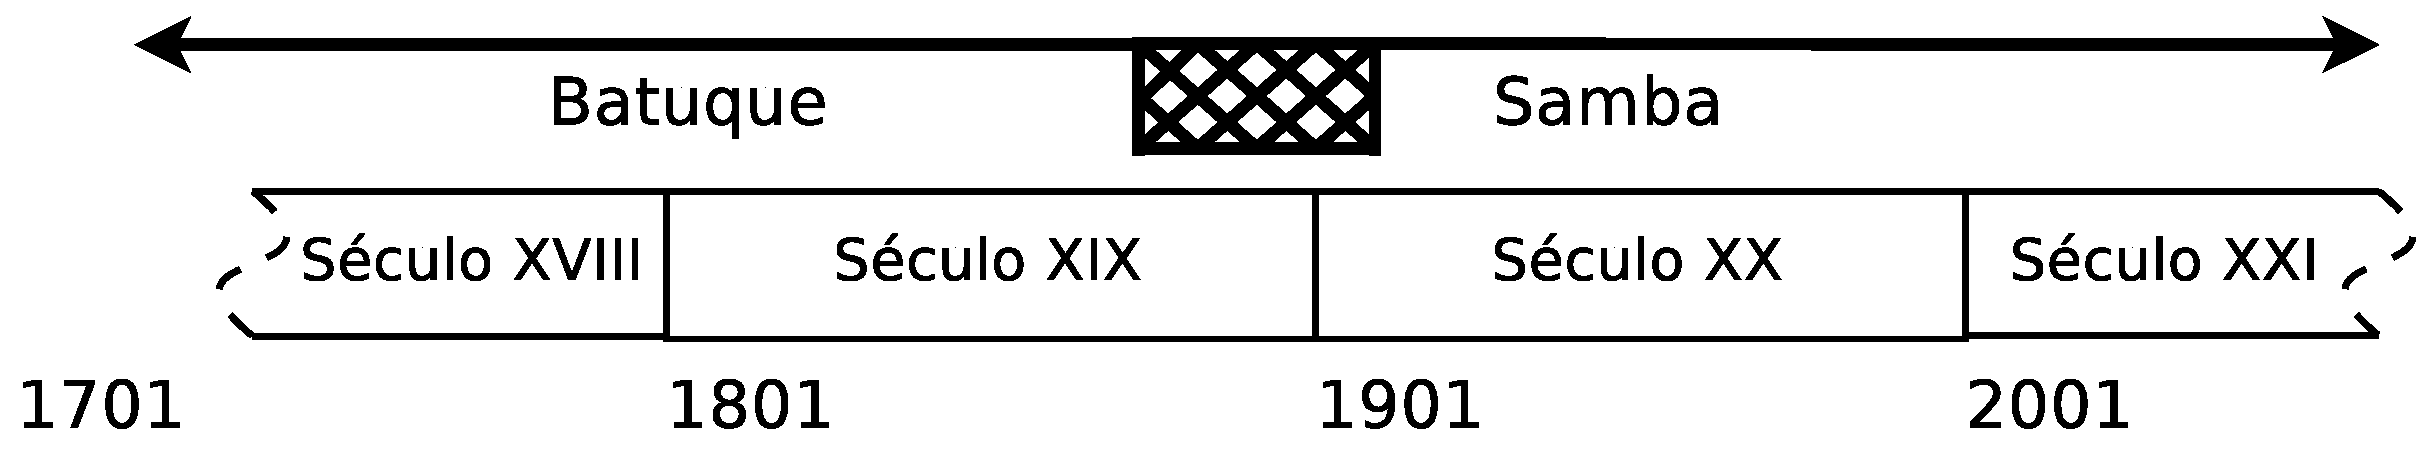
\includegraphics[width=1.0\textwidth]{chapters/cap-historia-samba/samba-crono.eps}
  \caption{Cronologia da designação geral dos festejos com danças, entendidas como com raiz africana.}
  \label{fig:sambacrono}
\end{figure}

\section{Expressões folclóricas relativas ao samba}

Para entender o folclore brasileiro, 
é importante ressaltar que o samba de roda, a batucada, 
o samba e o batuque são tipos gerais de dança afro-brasileira \cite[pp. 8]{reffolclorebatucadajornal} \cite[pp. 21]{jornalsambaderoda1}.
 
\begin{description}
\item [Samba de roda:]
\index{Samba de roda}
\index{Dança!Samba de roda}
\label{ref:Samba-de-roda-danca}
Também chamado, em 1936, \textbf{samba de morro} \cite[pp. 18]{jornalsambaderoda3}.
O samba de roda é uma manifestação cultural originaria da Baia 
que tem origem na dança dos negros do Brasil colonial (século XVII) \cite{unescosambaderoda1} \cite[pp. 21]{brasilpandeiro} \cite{silva2009capoeira},
esta se expandiu pelo Brasil todo e se popularizou nos estados de Rio de Janeiro e Pernambuco \cite{silva2009capoeira}.


No primeiro toque do tambor homens e mulheres se colocam a postos,
em circulo \cite[pp. 21]{brasilpandeiro} \cite{silva2009capoeira},
todo isto ao ritmo de orquestra de pandeiros, berimbaus, atabaque e agogô  \cite{silva2009capoeira}.
As pessoas passam ao centro e dançam individualmente ou em pares enquanto os demais batem palmas \cite[pp. 21]{brasilpandeiro}.
Um momento comum, em que a samba de roda e realizada é ao final das rodas da capoeira \cite{silva2009capoeira}.

Da união do \textbf{samba de roda} da Baia, com os ternos e ranchos de Reis, lusitano, 
e a música popular da época, 
nasceram as escolas de samba em Rio de Janeiro no segundo quartel no século XX \cite[pp. 8]{jornalsambaderoda4}

No ano 2008 o \textbf{Samba de Roda do Recôncavo Baiano} foi inscrito na ``Lista Representativa 
do Patrimônio Imaterial da Humanidade'' \cite{unescosambaderoda1}, indicando as seguintes caraterísticas para este estilo de roda:
\begin{citando}
Os participantes se reúnem em um círculo chamado roda. 
Geralmente, apenas as mulheres dançam. 
Uma por uma, elas vão se colocando no centro do círculo formado pelos outros dançarinos, 
que cantam e batem palmas ao seu redor. 
Essa coreografia frequentemente improvisada se baseia nos movimentos dos pés, 
das pernas e dos quadris.

Um dos movimentos mais característicos é a famosa umbigada (movimento de umbigo), 
de origem banto, pelo qual a dançarina convida quem vai sucedê-la no centro do círculo.
\end{citando}
 
%

\item [Samba-de-umbigada:]
\index{Samba-de-umbigada}
\index{Dança!Samba-de-umbigada}
\label{ref:samba-de-umbigada}
Entre as danças ``profanas'' %\cite[pp. 85]{sandroni2001feitico} 
afro-brasileiras o gesto da umbigada é um elemento muito 
caraterístico \cite[pp. 32]{jornalsambaderoda2} \cite[pp. 85]{sandroni2001feitico},
de modo que em 1961 Edson Carneiro definiu e englobou as danças que realizam este 
gesto como ``samba-de-umbigada''; assim, tradições 
musicais como o samba de roda, o jongo, o lundu, o coco, o calango e o cateretê, 
seguindo Edson são englobadas com  ``samba-de-umbigada'' \cite[pp. 85]{sandroni2001feitico}.

\item [Batuque (1900s):]
\index{Batuque!1900s}
\index{Dança!Batuque (1900s)}
\label{ref:batuquedanca}
É uma dança catalogada como pertencente ao folclore brasileiro  \cite[pp. 96]{sandroni2001feitico} e
é realizada em roda, na qual participam dançarinos, músicos e espectadores \cite[pp. 89]{marcondes1977enciclopedia}.
Chama-se ``baixão'' à introdução ou preludio da dança  e é executada pelo violeiro  \cite[pp. 89]{marcondes1977enciclopedia}.
No centro da roda fica um dançarino solista ou um ou mais pares
que se incumbem na coreografia \cite[pp. 89]{marcondes1977enciclopedia},
onde todos dançam de forma separada \cite[pp. 65]{sandroni2001feitico}.
A dança consiste num forte marcado pelos quadris, sapateados, palmas e estalar de dedos  \cite[pp. 89]{marcondes1977enciclopedia}.
É uma dança de \textbf{umbigada} \cite[pp. 96]{sandroni2001feitico} \cite[pp. 89]{marcondes1977enciclopedia}, 
onde o dançarino ou dançarinos solistas
dão \textbf{umbigadas} nos figurantes da roda  escolhidos para substitui-los \cite[pp. 89]{marcondes1977enciclopedia}.



\item [Batucada (1900):]
\index{Batucada}
\index{Dança!Batucada}
\label{ref:batucadadanca}
No inícios do seculo XX,
a ``batucada'' se distingue de outros sambas-de-umbigada por seu componente violenta, 
sendo esta executada principalmente por homens \cite[pp. 8]{reffolclorebatucadajornal} \cite[pp. 103]{sandroni2001feitico};
este era um jogo de destreza corporal, variante da capoeira e da samba-de-umbigada,
onde existiam \textbf{pernadas} que tinham o objetivo de derrubar ao parceiro, o qual, ao se manter em pé apos a pernada,
ganhava o direito de escolher o próximo parceiro
 e consequentemente tinha o privilegio de dar a próxima pernada nele \cite[pp. 103]{sandroni2001feitico}.

Baile que usa instrumentos de percussão onde se cantam versos que são respondidos pelo coro;
seguindo os mestres do gênero, de Rio de Janeiro, 
não há batucada com instrumentos de corda e de sopro, 
e  todas são feitas em roda \cite[pp. 89]{marcondes1977enciclopedia}.
A origem do baile é provavelmente africana; porem, alguns autores acham que pode ter origem em  danças indígenas,
basando-se nos desenhos dos livros de Théodore de Bry (1528-1598) e
nas informações de cronistas coloniais como Jean de Léry (1534-1611) e
Hans Staden (fl.1547-1556) \cite[pp. 89]{marcondes1977enciclopedia}.


\item [Batucada (outras acepções a partir de 1930):]
\index{Batucada}
\index{Dança!Batucada}
\label{ref:batucadadanca1930}

A palavra batucada ganhou outra conotação a partir dos anos 1930 \cite[pp. 103]{sandroni2001feitico}.

Depois de 1930, se retiravam do carnaval baiano, três clubes de elite por motivos econômicos; 
nesse contexto emergiram as batucadas que ritualizavam a presença da cultura afro-mestiça no carnaval; 
nesse período, a nível social e politico, a batucada e o samba eram considerados centrais no carnaval; 
porem, apos a década 1950, com o ressurgimento dos clubes de elite foi fechada a ``Era das Batucadas'' \cite{ICKES2013}.\\



Por outro lado, uma descrição interessante é dada no coro da música ``É batucada'', 
de Caninha e Visconde de Bicoiba (Bicohyba), no dia 18 de dezembro de 1932 \cite[pp. 12]{refebatucadajornal}.
\begin{citando}
Samba do morro\\
Não é samba, é batucada.\\
É batucada!\\
É batucada! Oi ...\\
\end{citando}
Caninha e Bicoiba indicavam com esses versos que na cidade (Rio de Janeiro),
o samba era privilegio dos compositores de espírito comercial, 
como Donga quando registrou pelo telefone em 1916 \cite[Cad. B pp. 4]{jornalsambaderoda5},
e que o resto de compositores que saiam do morro o que faziam era batucada 
(entendida na época como mais primitiva).\\




Finalmente, no vocabulário informal falado no morro (RJ em 1959), 
chama-se  ``batucada''
quando se trata de fazer humor ou satirizar alguma coisa \cite[pp. 32]{jornalsambaderoda2}.
\end{description}

%%%%%%%%%%%%%%%%%%%%%%%%%%%%%%%%%%
%% MARACATÚ
%%%%%%%%%%%%%%%%%%%%%%%%%%%%%%%%%%




%%%%%%%%%%%%%%%%%%%%%%%%%%%%%%%%%%%%%%%%%%%%%%%%%%%%%%%%%%%%%%%%%%%%%%%%%%%%%%%%
%% Capitulo
%%%%%%%%%%%%%%%%%%%%%%%%%%%%%%%%%%%%%%%%%%%%%%%%%%%%%%%%%%%%%%%%%%%%%%%%%%%%%%%%
\chapterimage{chapter_head_2.pdf} % Chapter heading image

\chapter{Historia das gafieiras}
\index{Historia das gafieiras}

%%%%%%%%%%%%%%%%%%%%%%%%%%%%%%%%%%%%%%%%%%%%%%%%%%%%%%%%%%%%%%%%%%%%%%%%%%%%%%%%
\section{Gafieira}
\label{def:Gafieira}
\index{Gafieira}
Atualmente o termo gafieira indica um baile de clube particular, com entrada paga e frequência livre. 

\begin{itemize}
\item \textbf{1979 em adiante:} Se entende que as gafieiras são locais de lazer 
e dança onde existe bom comportamento e muita compostura,
em perfeita integração racial; de modo que, 
a gafieira é sinônimo de baile em salão espaçoso como boa música orquestral \cite[pp. 10-11]{respeitojournalbrasil1}.

\item \textbf{1932 ate antes de 1979:} O termo gafieira foi associado a lugares de baixa ralé, onde 
se aconteciam frequentemente delitos e trágicos acontecimentos \cite[pp. 11]{gafieirajournalbrasil1} \cite[pp. 12]{gafieirajournaloradical1} \cite[pp. 10-11]{respeitojournalbrasil1}.

\item \textbf{1932:} popularização do termo gafieira, apos o
incidente entre o jornalista Romeu Arêde (Picareta) e o empresario e fiscal de salão Júlio Simões,
que provocou que  Picareta publica-se uma matéria apontando 
ao clube de Júlio como uma gafieira \cite[pp. 3 - cad. 3]{juliosimoes} 
\cite[pp. 21]{efege1974maxixe} \cite[pp. 78]{coutinho2006cronistas};
pelo que este último decidiu apelidar seu exitoso ``Elite clube'' como gafieira;
espalhando-se rapidamente esta denominação a outros clubes similares. 
Assim, o termo queda vinculado a clubes de dança da classe média,
onde eram aceitos todas as pessoas sem nenhum tipo de preconceito racial, 
prévio pago da entrada \cite[pp. 6 - cad. B]{entrevistajuliojournalbrasil1}.


\item \textbf{1917 ate 1932:} 
Inícios do uso do termo gafieira, indicando bailes populares \cite[pp. 29]{instituto1987revista} de entrada paga
ou bailes criados por motivo do carnaval; sendo que, as referencias bibliográficas
achadas são nas semanas próximas ao carnaval \cite[pp. 4]{oldgafieira1} 
\cite[pp. 7]{oldgafieira2} \cite[pp. 4]{oldgafieira3} \cite[pp. 5]{oldgafieira4},
o que mostra a notoriedade que adquiriam esses eventos, ou locais, nessas datas.
\end{itemize}

%%%%%%%%%%%%%%%%%%%%%%%%%%%%%%%%%%%%%%%%%%%%%%%%%%%%%%%%%%%%%%%%%%%%%%%%%%%%%%%%
\section{Cronologia das gafieiras}


%%%%%%%%%%%%%%%%%%%%%%%%%%%%%%%%%%%%
%\PRLsep{Bailes na década de 1800}

Seguindo o jornalista Agostinho Seixas,
entre os anos de 1847 e 1848, na Cidade Velha, no Rio de Janeiro,
já existiam  bailes e clubes recreativos, 
que hoje denominaríamos como \textbf{gafieiras} \cite[pp. 11]{respeitojournalbrasil1}.
Seixas achou como primeira referencia na suas pesquisas, que entre essas datas,
Dona Francisca Pacheco da Silva, fazia um requerimento 
à ``Excelentíssima Câmara'' (que foi concedido) para a autorização 
da sua sala de bailes, na Rua da Alfândega, 327 \cite[pp. 11]{respeitojournalbrasil1} \cite[pp. 71]{perna2002samba};
este requerimento foi catalogado como sala de danças, 
com a característica de ter entrada paga.
Seguindo o fiscal que acompanhava o requerimento,
ele não achava artigo que regulamentasse esse tipo de local 
de diversão ou dança; lembremos que nessa época
o padrão era ter clubes fechados que tinham um determinado número de sócios \cite[pp. 11,12]{respeitojournalbrasil1}.



%%%%%%%%%%%%%%%%%%%%%%%%%%%%%%%%%%%%
\PRLsep{Bailes na década de 1900}


Para inícios do século XX, podiam ser achadas varias associações para negros e mestiços, 
com distintas  finalidades, como: sociedades beneficentes, literárias, dramáticas, esportivas 
e as ``sociedades dançantes e recreativas'' abertas a um público geral
\cite[pp. 154-155]{neres1999negro} \cite[pp. 71]{de2008bexiga}.
Estas associações geralmente não tinham local próprio, 
e tinham que alugar espaços que terminavam sendo salões de velhos sobrados
ou similares \cite[pp. 154-155]{neres1999negro} \cite[pp. 49]{diniz2003almanaque}.
Entre as organizações sociais recreativas mais comuns da época tínhamos, 
os cordões\footnote{Os cordões eram grupos festivos de dança e música, 
com pessoas mascaradas com figurinos de reis, de
bichos, de pajens, de guarda, etc., tocando instrumentos africanos \cite[pp. 23-24]{fernandes2001escolas}},
os ranchos\footnote{Quando os cordões desapareceram estes se transformam em ranchos (depois de 1908), 
agregaram instrumentos de corda e metais, e inciou a ser tocado a marcha-rancho,
os ranchos eram cordoes mais civilizados \cite[pp. 24]{fernandes2001escolas}} 
e os zé-pereiras\footnote{ Uma sociedade recreativa do ``Ze-pereira''
é uma sociedade dedicada a dança carnavalesca \cite[pp. 10]{simoesjournalbrasil1}} 
\cite[pp. 10]{simoesjournalbrasil1}.


Uma destas sociedades de dança do inícios do seculo XX, que agora definiríamos como gafieira, 
foi a ``Sociedade de Danças Clovis Invencivel''\footnote{Em algumas versões 
``Clovis Invencivel'' é referenciado como ``Clowns Invencíveis'' \cite[pp. 3 - cad. 3]{juliosimoes} ou 
``Clovis Invencíveis'' \cite[pp. 10]{simoesjournalbrasil1}}, 
esta foi fundada no Rio de Janeiro em 1906, 
na qual eram populares concursos de valsa, polca ou quadrilha \cite[pp. 6 - cad. B]{entrevistajuliojournalbrasil1}.
O dono da ideia da criação destes concursos foi um muito jovem e fiscal do salão, Júlio Simões,
que a seus 16 anos pensou numa sociedade de dança diferente dos da época,
que se dedicavam a ``bater bumbo'' (bailes carnavalescos ou de zé-pereira), 
a uma dedicada a ``arrasta-pés'' (bailes de salão) 
\cite[pp. 6 - cad. B]{entrevistajuliojournalbrasil1} \cite[pp. 3 - cad. 3]{juliosimoes} \cite[pp. 10]{simoesjournalbrasil1}.

Com o surgir dos lugares de baile, em 1915 \cite[pp. 1 - cad. B]{gafieira2000reis},  
Júlio Simões, foi chamado pelos sócios\footnote{Os 
sócios fundadores da ``Kanaga do Japão'' são José Constantino da Silva 
e José de Paiva Brito \cite[pp. 1 - cad. B]{gafieira2000reis}} da ``Kanaga do Japão'' para dirigir seu novo clube,
lugar de grande tradição no Rio de Janeiro, e muito popular na época,
no qual o conjunto encarregado de animar o local era chefado por Sinhô e Bulhões de Carvalho,
que receberam o título popular de ``reis da valsa'',
com torneios de dança que duravam ate 55 
minutos dançando uma valsa rápida \cite[pp. 3 - cad. 3]{juliosimoes} \cite[pp. 1 - cad. B]{gafieira2000reis} \cite[pp. 6 - cad. B]{entrevistajuliojournalbrasil1}.
Nas festas comandadas por Júlio, era comum ver dançar samba, polca, 
valsa e quadrilha, que ele mesmo marcava no salão \cite[pp. 1 - cad. B]{gafieira2000reis}. 


Para o ano 1930, estas sociedades dançantes tinham ganhado muita popularidade. 
Assim, apos a morte de um socio e o fechamento da ``Kananga do Japão'' 
em 1929 \cite[pp. 3 - cad. 3]{juliosimoes}  \cite[pp. 11]{eliteinaugura} \cite[pp. 1 - cad. B]{gafieira2000reis}, 
Júlio Simões procura a Heitor Persegani e  Hilário Jovino, 
e decidem fundar o local de danças chamado ``Elite club'' \cite[pp. 11]{eliteinaugura} \cite[pp. 13]{respeitojournalbrasil1},
agora chamado ``Elite clube'' \cite[pp. 3 - cad. 3]{juliosimoes},
na Rua Frei Caneca n. 4 - Centro, Rio de Janeiro - RJ;
sendo o 17 de julho de 1930 seu baile inaugural 
\cite[pp. 11]{eliteinaugura} \cite[pp. 3 - cad. 3]{juliosimoes} \cite[pp. 10]{simoesjournalbrasil1}.

Uma descrição de uma destas sociedades dançantes, anterior a 1931, pode ser vista no livro "O cabrocha"; 
escrita  por Jota Efegê em 1931; 
sobre a ``Sociedade Recreativa Familiar Bohemios de Botafogo'' \cite[pp. 24-26]{jotaefege},
a continuação é mostrado um extracto desse texto:
\begin{citando}%%
O salão, comquanto não fosse de grandes dimensões, era
de um tamanho regular, confinando com uma pequena saleta
onde tambem se dansava; estava bem affluido. Numa
heterogeneidade foliã, via-se desde a crioulinha blasée, sem
elegancia, desalinhada, á mulatinha pernostica de faces
avermelhadas por um carmin berrante, cabello engommado e
subjugado por travessas e grampos, num á la garçonne
forçado, mas exigido pela moda. Em meio dessas "cabrochas"
e "roxinhas", viam-se algumas moças brancas de apparencia
sobria. São as meninas que não podem fazer um vestido de
seda ou calçar sapatos de setim, para se apresentarem no
Fluminense ou no Flamengo e que nestes clubes se divertem,
ficando em evidencia por serem brancas.  %~\\
(Jota Efegê)
\end{citando}

%%%%%%%%%%%%%%%%%%%%%%%%%%%%%%%%%%%%
\PRLsep{Inícios do uso do termo gafieira}

Fazendo uma pesquisa na ``Biblioteca Digital da Fundação Biblioteca Nacional''
podemos achar referencias ao termo \textbf{gafieira} desde 1917\footnote{Mesmo 
ano em que foi lançado o samba ``Pelo telefone'', sendo um exito total no carnaval desse ano.}.


A primeira referencia pode ser vista no jornal ``O Imparcial'' (RJ),
do dia 17 de janeiro de 1917, como o título ``Batalha de confetti'',
no qual se anuncia que na rua Guimarães se terá uma grandiosa batalha,
organizada pelo ``bloco dos pesados'', conformado por \cite[pp. 4]{oldgafieira1} \cite[pp. 629]{spielmann2016reflexoes}:
\begin{citando}
Lourenço dos Santos (Lord Sorvete),\\
Antonio dos Santos (Lord Massa),\\
Antonio Lima (Lord Repinica),\\
Raul Dantas (Lord Ronqueira),\\
Almeidinha (Lord Prrrrr...!),\\
Arlindo dos Santos (\textbf{Lord Gafieira}),\\
Joaquim Mello (Lord Frango d'Agua),\\
Juvenal Branco (Lord Pé Pequeno),\\
Eudoxio dos Santos (Lord Garganta) e\\
Jorge Vença (Lord Come Bola).
\end{citando}
Pelo contexto do anuncio, e pela semelhança com os outros apelidos, 
pode-se perceber que o termo \textbf{gafieira} tem um significado alegre,
cotidiano ou extravagante, mas é difícil extrair alguma outra conclusão.

A seguinte referencia aparece um ano depois, no mesmo jornal,
no dia 8 de fevereiro de 1918, como o título ``Grande batalha de confetti'',
na qual se anuncia que a batalha é organizada pelo ``bloco da rapaziada'',
do ``\textbf{Club da Gafieira}'', a qual também terá a participação 
da \textbf{orquestra do ``Gafieira''} que tocará adoráveis tangos;
e se finaliza falando que  \cite[pp. 7]{oldgafieira2} \cite[pp. 629]{spielmann2016reflexoes}:
\begin{citando}
Serão distribuídos brindes áquelles que mais se têm distinguido nos bailes do valoroso ``\textbf{Gafieira}''.
\end{citando}
Nesta referencia, já podemos observar que a palavra gafieira é relativa à celebrações do carnaval, 
e a lugares ou eventos de bailes,
nos quais, por exemplo, se dançam tangos; 
pelo que a palavra \textbf{gafieira} é usada no nome da orquestra,
e no apelido de um integrante, o valoroso \textbf{Gafieira}.

Um ano depois na ``Gazeta de Noticias'' (RJ),
no dia 3 de março de 1919, com o título ``Club dos carnavalescos do Andarahy'' e subtitulo ``1ra Critica - A Gafieira'',
se anuncia que a ``Banda de clarins'' e a ``Banda de música'',
tocarão uma espirituosa ``charge'' aos bailes de clubs de mil réis por cabeça, 
na qual era  usada a seguinte letra \cite[pp. 5]{oldgafieira3} \cite[pp. 629]{spielmann2016reflexoes}:
\begin{citando}
Cinco tostão vale a varsa!\\
Grita o fiscal do salão:\\
Tirem as dama depressa,\\
Não perquem a casião!\\ ~\\
Sapeca o piston com força,\\
Requebra mais, já se vê!\\
Que depois da contradança,\\
A dama vai p'r'o bufê.\\ ~\\
Paga a entrada e não estrilla!!\\
Que isto aqui é uma deliça!\\
Se porte bem, seu varsista!\\
Cuidadinho e'n a poliça!...
\end{citando}
Nesta última referencia já podemos ver claramente o sentido do termo gafieira,
identificando a um lugar de dança, em especifico a esses lugares com entrada paga a mil réis por cabeça.
Para ter uma ideia de se este preço é pouco ou muito, podemos compará-lo com o 
preço do jornal em que foi publicado o texto, sendo este de 100 RS \cite[pp. 1]{oldgafieira3};
ou também por essas épocas, 
quando a entrada custava 2 mil réis o preço de uma cerveja  era  de 800 réis \cite[pp. 1 - cad. B]{gafieira2000reis}.
Outro dado interessante é o uso do termo ``fiscal de salão'', 
figura de autoridade que já estava presente 
nas sociedades dançantes do seculo XX, como por exemplo na 
``Sociedade de Danças Clovis Invencivel'' em 1906, pelo que queda claro
a que lugares se refere o termo gafieira.


Podemos ver outra noticia relativa as gafieiras, no dia 19 de janeiro de 1920, 
no jornal ``A Razão'' (RJ), no qual se
publica uma reportagem com o título 
``Charivari num club suburbano - Fechado pela policia'',
se referindo ao clube ``Fenianos de Cascadura'',
que seguindo o descrito, este clube era 
ponto de reunião de gente desclassificada, 
que realizava seus bailes os sábados e domingos,
cobrando na entrada $1\$100$ por cabeça.
O seguinte texto é uma porção daquela reportagem \cite[pp. 4]{oldgafieira4} \cite[pp. 629]{spielmann2016reflexoes}:
\begin{citando}
A policia local, que é a do $20^o$ districto,
já estava farta do trabalho que o club 
constantemente lhe dava e de receber reclamações 
dos moradores visinhos.\\
Deliberou então o delegado, dr. Coelho
Gomes, fechar o club, mais conhecido por 
``\textbf{Gafieira}'', na primeira occasião que `e apresentasse.\\
Ante-hontem, sabbado, á noite, o club 
deu o acostumado ``baile'' e ás 5 horas da 
madrugada houve, ali um ``charivari'' medonho,
que poz o largo de cascadura em polvorosa. 
\end{citando}
O termo charivari se usa para indicar música discordante, 
confusão, motim, tumulto, barafunda \cite[pp. 53]{almeida1996dicionario}, etc.
Assim, podemos ver como o termo gafieira, 
estava relacionado a clubes de dança com entrada paga,
e que era frequentado por pessoas de poucos recursos econômicos. 
Também é interessante ressaltar que as referencias achadas correspondem,
a datas próximas ao carnaval, o que mostra o vinculo ou o maior interesse 
destes locais nestas datas. 

Ainda podem ser achadas outras referencias ao termo \textbf{gafieira} na década de 1920,
nelas podemos destacar apelidos usados por professores de dança,
ou referencias de musicas com letras indicando que gafieiras 
são frequentadas por crioulas e/ou criadas.


%%%%%%%%%%%%%%%%%%%%%%%%%%%%%%%%%%%%
\PRLsep{Popularização do termo gafieira}

Seguindo o jornalista e cronista, Jota Efegê, %%Júlio Simões e o historiador,
o termo ``gafieira'' foi criado pelo cronista carnavalesco, 
Romeu Arêde\footnote{Em algumas versões está  referenciado como Romeu Aredo \cite[pp. 188]{raca1999}.}, 
também conhecido como ``Picareta'' \cite[pp. 29]{instituto1987revista}\cite[pp. 3 - cad. 3]{juliosimoes} 
\cite[pp. 21]{efege1974maxixe} \cite[pp. 78]{coutinho2006cronistas}, 
colunista da seção recreativa do ``Jornal do Brasil'' desde 1930 ate 1941
e anteriormente do vespertino ``Vanguarda'' (1922-1930) \cite[pp. 58-59]{efege1982figuras} 
\cite[pp. 6 - cad. B]{entrevistajuliojournalbrasil1};
porém não é indicada, por Jota Efegê, referencia nenhuma sobre a data de criação.
Efegê indica que o termo ``gafieira'', possivelmente deriva de 
``cabroeira''\footnote{Cabroeira: Malta de indivíduos chamados cabras, 
de capangas assalariados para assassinar ou para fazer o mal \cite{diciocabroeira}.} 
ou ``gaforinha'' \cite[pp. 3 - cad. 3]{juliosimoes}.
Por outro lado, Júlio Simões, socio e administrador do ``'Elite club', 
afirma\footnote{Seguindo a ``Revista do Instituto Histórico e Geográfico do Rio de Janeiro'' (1987),
Jota Efegê afirma que foi Romeu Arêde quem atrelou o termo gafieira aos clubes de dança no incidente no ``Elite clube''.} 
que o jornalista Romeu Arêde tinha a costume de entrar, 
comer, beber, dançar e não pagar \cite[pp.13 ]{respeitojournalbrasil1},
e que quando ele impediu ao boêmio jornalista e seus acompanhantes (5 ou 6) o ingresso no ``Elite'', 
porque a entender de Júlio o jornalista estava meio ``alegre'' devido a uns tragos a mais;
 Júlio indicou: ``Aqui tem ordem'' 
\cite[pp.13 ]{respeitojournalbrasil1} \cite[pp. 6]{gafieiraaredeout2} \cite[pp. 3 - Encontro]{gafieiraaredeout1},
indicando que só podiam passar com entrada franca ele mais uma dama ou um amigo;
o cronista então reagiu indicando a seus acompanhantes a se retirarem, 
exclamando \cite[pp. 29]{instituto1987revista} \cite[pp. 6 - Tribuna Bis]{gafieiraaredeout3}: 
\begin{citando}
Vamos embora! Isto aqui é uma gafieira!
\end{citando}
Outras referencias apontam que o que falou foi \cite[pp. 6]{gafieiraaredeout2} \cite[pp. 3 - Encontro]{gafieiraaredeout1}:
\begin{citando}
O que eu vou fazer nessa gafieira?
\end{citando}
Ao dia seguinte Picareta escreveria na sua coluna no Jornal do Brasil \cite[pp. 188]{raca1999}:
\begin{citando}
Aquele é um lugar da ralé, onde se cometem gafes em fieiras
\end{citando}
Varias referencias apontam que este incidente aconteceu em 1932 \cite[pp. 3 - Encontro]{gafieiraaredeout1} \cite[pp. 188]{raca1999}, 
porém não se menciona o dia exato. 




Assim, em qualquer das explicações da formação da palavra gafieira,
seja por ``cabroeira''+``gaforinha'' ou ``gafes''+``fieira'',
esta era uma denominação pejorativa para indicar a um local (``cabroeira'' ou ``gafes'').
É importante lembrar que o termo \textbf{gafieira}, já existia desde antes do 
incidente entre Júlio Simões e Romeu Arêde no ``Elite club'', 
especificamente se tem constância do uso desde 1917 \cite[pp. 4]{oldgafieira1},
pelo que para a data da apertura do ``Elite club'' em 1930,
este termo já estava no consciente de algumas pessoas, porém não estava popularizado;
pelo que se deduz que Romeu Arêde, por conta do incidente no ``Elite club'', 
atuou como catalisador para a popularização do termo gafieira.
%mas isto não descarta a informação de Jota Efegê que indica que foi Arêde quem criou o termo,
%pois  Efegê não menciona uma data especifica.

Júlio simões apos o incidente no ``Elite club'', 
decide devolver a piada e apelidar seu local como 
``Gafieira'', conservando o nome de clube, 
mas transformando-se na pratica em ``Gafieira Elite'' \cite[pp. 79]{moura1995tia} \cite[pp. 6 - Tribuna Bis]{gafieiraaredeout3}.
Por este incidente e suas repercussões, 
muitos autores consideram a ``Elite'' como a primeira gafieira do Brasil \cite{cabral2016elisete} \cite[pp. 84]{cabral1996escolas}.
Consequentemente, e em palavras de Jota Efegê, 
se considera a Júlio Simões como o criador das gafieiras \cite[pp. 3 - cad. 3]{juliosimoes}.

Nesse ponto da historia, 
o nome ``gafieira'' cobrou muita relevância e locais de dança apelidados como gafieiras surgiram no Rio de Janeiro;
depois de tudo, já existissem lugares com estas caraterísticas desde inícios do século XX \cite[pp. 49]{diniz2003almanaque}.
Os salões foram criadas a semelhança dos bailes de salão da classe média ou alta \cite[pp. 78]{coutinho2006cronistas}; 
porém, no caso das gafieiras, estas eram abertas ao público prévio pago da entrada.
A Figura \ref{fig:gafieiracrono} mostra a cronologia do uso da palavra gafieira para os salões de dança no Rio de Janeiro.
\begin{figure}[h]
  \centering
    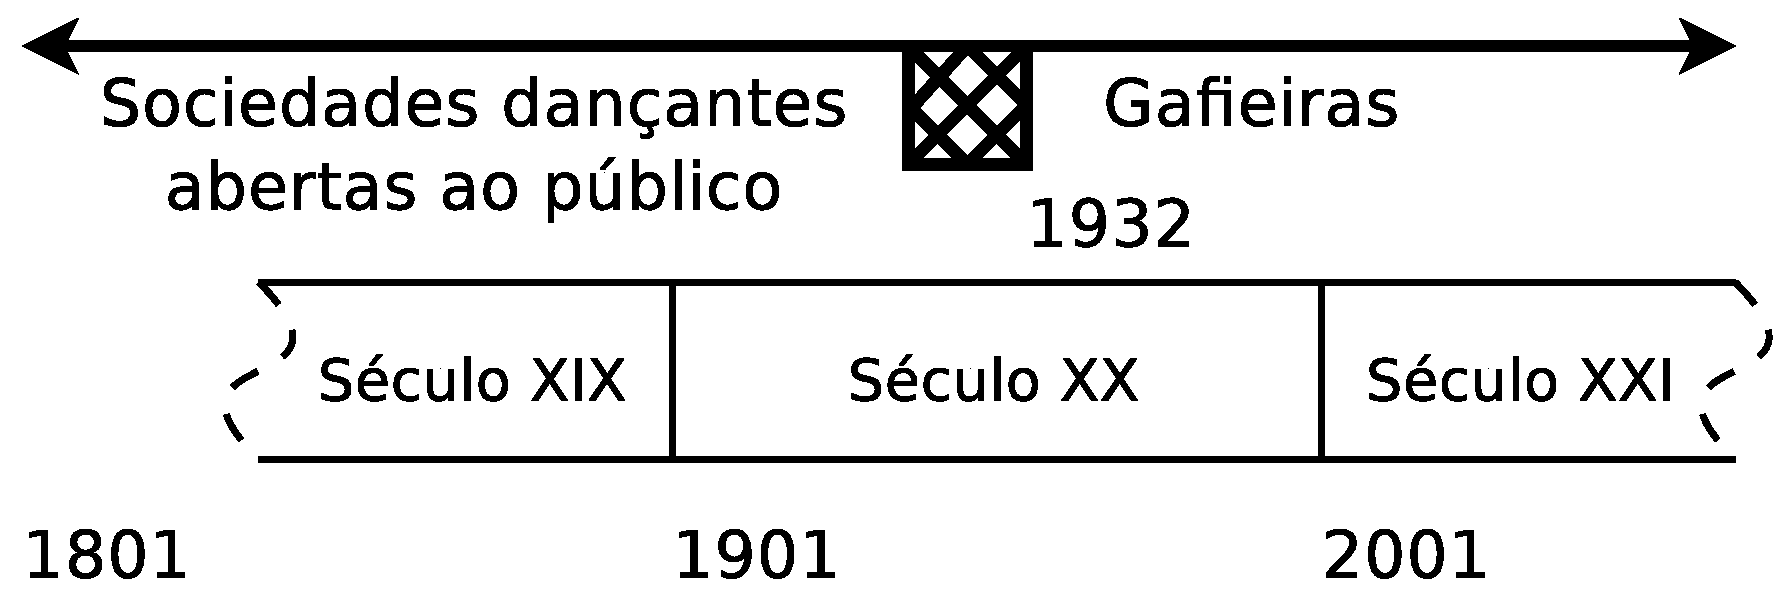
\includegraphics[width=1.0\textwidth]{chapters/cap-historia-gafieiras/gafieira-crono.eps}
  \caption{Cronologia da designação de gafieira para os salões de dança no Rio de Janeiro.}
  \label{fig:gafieiracrono}
\end{figure}

\PRLsep{Delitos vinculados com as gafieiras}

Podemos achar uma referencia ao termo gafieira no jornal ``O Radical'' (RJ),
no dia 8 de setembro de 1932 \cite[pp. 12]{gafieirajournaloradical1},
com o titular:
\begin{citando}%%
A sahida do baile: Por causa de Aracy, o estivador foi ferido á baia.\\
... Na rua Domingo Lopes, n. 243, em Madureira, está situado o club de dança Ideal, 
conhecido pelos moradores locaes por ``Gafieira''.
\end{citando} 
Ao dia seguinte, 9 de setembro de 1932, o jornal ``A Batalha'' (RJ), 
usava também a palavra ``gafieira'' para se referir ao mesmo incidente \cite[pp. 8]{gafieirajournalabatalha1}.

O ``Jornal do Brasil'', o dia 9 de janeiro de 1934, 
usa também a palavra gafieira \cite[pp. 11]{gafieirajournalbrasil1}, com o titular:
\begin{citando}%%
À porta de uma ``gafieira''.
Ainda o conflito da madrugada de domingo no largo de Madureira.
Faleceu um dos soldados no Hospital da Policia Militar. 
Ha no largo de Madureira uma sociedade dansante, mais conhecida por ``gafieira'', 
com entradas retribuidas, ondem de quando em quando, se registram conflitos, 
alguns de graves consequências...
\end{citando} 
Como é visto nas refecerias antes mostradas, e guardando semelhança com outras coincidências
posteriores que podem ser achadas na ``Biblioteca Digital da Fundação Biblioteca Nacional''; 
o termo gafieira, estava associado a lugares considerados perigosos;
isto propiciado pelo aumento do número de locais que se atribuíam este nome, junto com 
a diversidade e cultura  do seu público e administradores.
Porém, este não seria o padrão pelo qual se regiam todas as gafieiras, 
e certamente a conotação mais perigosa ou pejorativa iria mudando no tempo. 

\PRLsep{A gafieira limpa seu nome}

Por exemplo, sobre o Elite Club,  nos sabemos que funcionava as quintas, sábados e domingos,
e existia um fiscal no salão (o velho Russo)\cite[pp. 37]{gafieirajournalmanchete}, 
que fazia cumprir estritamente as normas de bom-tom, comportamento social e respeito ao ambiente, como todo clube familiar precisa ter \cite[pp. 12]{respeitojournalbrasil1}; de modo que, 
não eram admitidas damas que não estivessem de sapatos de salto alto \cite[pp. 37]{gafieirajournalmanchete};
homens embriagados não entravam e o traje indispensável era o paletó e gravata, 
ou no mínimo camisa fechada \cite[pp. 6 - cad. B]{entrevistajuliojournalbrasil1}.
O cavaleiro não podia abraçar a dama nem sentado na cadeira \cite[pp. 6 - cad. B]{entrevistajuliojournalbrasil1},
né dançar de rosto colado, ou por a mão nas costas da dama sem usar lenço \cite[pp. 10]{simoesjournalbrasil1}, 
quem fiscalizava, na porta, era um preto velho tratado por todos de ``titio''  \cite[pp. 37]{gafieirajournalmanchete}.
Se alguma regra não era cumprida, o seu Júlio, jogava a qualquer um para fora \cite[pp. 6 - cad. B]{entrevistajuliojournalbrasil1}.
Nos bailes dedicados ao padroeiro, todo 20 de janeiro, era obrigatório vestir de branco,
já seja no traje ou no vestido, incluindo sapatos e camisas \cite[pp. 37]{gafieirajournalmanchete}.
Tão grande era o censo de ordem dos frequentadores do Elite Club, 
que lhe era permitido operar estando a menos de 80 metros de um hospital,
sendo que nessa época existia a Lei n. 1.590 de 1924, 
seguindo a qual nenhuma casa de diversões podia estar a menos de 200 m de estabelecimentos hospitalares,
Ate o próprio Delegado Dulcídio Gonçalves, da Delegacia de Costumes,
dispensava-se de mandar policiar o Elite.
``À casa do Júlio não precisa de policiamento'', dizia o Delegado Dulcídio
\cite[pp. 5]{simoesjournalalutademocratica1}.


Assim, ao transcorrer dos anos, essa visão popular mais obscura da palavra gafieira foi mudando;
pelo qual o jornalista Francisco Duarte, o dia 12 de agosto de 1979,
escreve no Jornal do Brasil (RJ) sobre este assunto com o título:
``Gafieira - Tratado geral do ambiente que exige respeito'' \cite[pp. 10]{respeitojournalbrasil1}:
\begin{citando}%%
... o verbete Gafieira com o significado de baile reles, arrasta-pé, baile popular de baixa categoria.
No passado, encarada com má vontade pelos puristas do léxico e pela burguesia republicana dançante,
pode ter sido assim. Mas em 1979 -- e cabe aos dicionaristas verificar in loco --
gafieira é baile de clube particular, com entrada paga e freqüência livre, 
local de lazer e dança onde existe bom comportamento e muita compostura,
em perfeita integração racial.\\
(Francisco Duarte)
\end{citando}
Além da afirmação anterior, 
o jornalista explica como a ``Delegacia de Diversões Públicas'' classifica as casas de dança;
assim temos: 
\begin{itemize}
\item ``boates'', que são bar restaurantes com pista de dança e palco para show;
\item ``cabarés'', onde se bebe, come, dança e se tem espetáculos de variedades;
\item ``dancings'' onde se dança mediante pagamento em cartões e picotes; e 
\item ``inferninhos'' que são boates de baixa categoria, 
frequentados por pessoas de vida irregular e onde se toca música barulhenta.
\end{itemize} 
Em palavras de Duarte, ``Gafieiras são sinônimos de baile em salão espaçoso como boa música orquestral'' \cite[pp. 11]{respeitojournalbrasil1}.




%%%%%%%%%%%%%%%%%%%%%%%%%%%%%%%%%%%%%%%%%%%%%%%%%%%%%%%%%%%%%%%%%%%%%%%%%%%%%%%%
%% SUB SECTION
\section{Estatutos da gafieira}\index{Estatuto da Gafieira}
Os ``Estatutos da Gafieira'' é uma composição musical escrita, por Billy Blanco;
esta foi interpretada por primeira vez na voz de Inezita Barroso, 
numa gravação da "RCA Victor" em janeiro de 1954 \cite{musicaestatuto};
O seguinte texto mostra a letra da música numa 
versão publicada no jornal ``Cinelândia''  (RJ),
na segunda quinzena de dezembro de 1955 \cite[pp. 95]{musicaestatutojournal1955}.
\begin{citando}%%
\center{Moço! Olha o vexame!}\\
O ambiente ``ingige'' respeito!\\
Pelos estatutos da nossa gafieira\\
Dance a noite inteira, mas dance direito!\\
Aliás, pelo artigo 120,\\
O cavalheiro que fizer o seguinte:\\
Subir nas paredes, dançar de pé pro ar,\\
Morar na bebida sem querer pagar,\\
Abusar da umbigada de maneira folgazã,\\
Prejudicando hoje o bom crioulo de amanhã,\\
Será distintamente censurado!\\
Se balançar o corpo, tá na mão do delegado!\\
Balançou o corpo? tá na mão do delegado!\\
\end{citando}
O texto é uma tentativa bem-humorada do autor de descrever o que acontecia 
nas gafieiras, porém na época da escrita desta popular samba, não
existiam tais estatutos\footnote{Estatutos, no sentido de regulamento, 
ordenança o conjunto de normas legais pelas que se regula o funcionamento de uma corporação ou associação.};
existia um código de costumes sim \cite[pp. 13]{respeitojournalbrasil1} em alguns salões, 
mas cada casa de dança imponia estes no seu local a critério do fiscal do salão ou dos 
donos \cite[pp. 10]{simoesjournalbrasil1} \cite[pp. 6 - cad. B]{entrevistajuliojournalbrasil1} \cite[pp. 37]{gafieirajournalmanchete},
isto é confirmado por um depoimento realizado por 
Billy Blanco no 8 de julho de 2011 \cite[pp. 56]{depoimentobilly}; o texto a seguir
mostra um fragmento dessa entrevista.

\begin{citando}%%
"Observando os acontecimentos de uma gafieira, então, eu imaginei
coisas, porque o compositor vive muito da imaginação. E eu criava situações 
possíveis de serem acontecidas na gafieira, ou então narrava o que
acontecia realmente. Por exemplo, no [samba] Pistom de Gafieira, tinha
um cidadão que era pistonista da orquestra que sempre tocava forte para
disfarçar quando a polícia vinha chegando. Doutra feita, eu tive a ideia
de fazer o estatuto para a gafieira. Então eu humorizei, porque ninguém
dança de pé pro ar, nem sobe em parede, não é? Mas a gente cria uma
extravagância dessas para dar uma certa graça, um certo sentido à música.
Na época, não havia código nenhum, eu apenas criei aquilo e muitas gafieiras 
depois tinham esse estatuto na parede para quem quisesse cantar.
Você vê que as regras do estatuto são umas regras brincalhonas, não é?" 
~\\
(Billy Blanco)
\end{citando}

Mesmo observando que as regras propostas pelo autor tem um caráter humorístico e sarcástico,
o texto foi adotado rapidamente pelas gafieiras, como um chamado a reflexão sobre umas
normas básicas a serem tidas em conta no salão, pois tem um grau de bom senso. Por exemplo: 
A linha 7, pode ser interpretada como uma indicação a 
não fazer movimentos aéreos na pista de dança,
ou  evitar movimentos capoerísticos; tudo isto
pelo evidente espacio reduzido e compartilhado que existe na pista de dança, 
além de que os movimentos aéreos estão pensados para ser
executados em apresentações e não em danças sociais. 
A linha 8, nos lembra o respeito ao parceiro; pois a pessoa que dança precisa
estar no controle de suas faculdades físicas e mentais; 
no caso dos \hyperref[def:Condutor]{\textbf{condutores}}\footnote{\label{footlab:conducao}Nas danças sociais é comumente usado o paradigma da condução; 
no qual, no casal, uma pessoa assume o papel de \hyperref[def:Condutor]{\textbf{condutor}} dos movimentos e 
a outra pessoa assume o papel de \hyperref[def:Seguidor]{\textbf{seguidor}}, este recebe a informação da condução e retorna uma resposta corporal.}, 
para estar atentos ao salão e cuidar do seu par enquanto os movimentos são executados, 
e no caso do \hyperref[def:Seguidor]{\textbf{seguidor}}\footref{footlab:conducao} para evitar problemas
nos giros e outros movimentos que precisem  controle do eixo do corpo.
As linhas 9 e 10 indicam sobre um conjunto de expressões artísticas 
afro-brasileiras emolduradas no século XIX com o nome de ``samba umbigada'' \cite[pp. 47]{diniz2008almanaque} \cite[pp. 85]{sandroni2001feitico}; nestas danças existe
um movimento chamado ``umbigada'' \cite[pp. 50]{da2015historia} que dá nome à dança, na qual o ventre do homem e da mulher batem geralmente para indicar
a troca de dançarino; assim as linhas 9 e 10 se referem a
 evitar ``abusar'' de movimentos de umbigada que provem de danças que não eram bem vistas na época e eram consideradas gentílicas \cite[pp. 85]{sandroni2001feitico}.
Finalmente,
a linha 12 fala sobre balançar o corpo, que seguindo o contexto cultural, 
pode indicar não agir como bêbado\footnote{``Balançar o corpo; agitar, como o bebado, mal firme, e outros táes'', Diccionario da lingua portugueza, 1858 \cite[pp.296]{diccionario1858}.}, ou em outras palavras,
com pouca elegância ou respeito,
caso contrario seria levado à delegacia!.



%%%%%%%%%%%%%%%%%%%%%%%%%%%%%%%%%%%%%%%%%%%%%%%%%%%%%%%%%%%%%%%%%%%%%%%%%%%%%%%%
%% Capitulo
%%%%%%%%%%%%%%%%%%%%%%%%%%%%%%%%%%%%%%%%%%%%%%%%%%%%%%%%%%%%%%%%%%%%%%%%%%%%%%%%
\chapterimage{chapter_head_2.pdf} % Chapter heading image

\chapter{Historia da música do samba}\index{Música do samba}

O samba é uns dos gêneros musicais mais conhecidos no Brasil do século XXI;
entre estes gêneros mais populares, temos por exemplo, ao ``forró'' e ao ``Sertanejo'';
sendo que o samba se distingue entre eles, 
como a principal expressão popular da música brasileira \cite[pp. 47]{diniz2008almanaque}.\\


%\begin{definition}[Samba:]
\begin{tcbremarcar}
\textbf{Samba:}
\index{Samba}
\label{ref:samba} 
No Brasil, a palavra samba  é usada como designação de uma dança popular  e música  em compasso binário (basicamente 2/4), 
de ritmo sincopado e andamento variado \cite[pp. 290]{dourado2004dicionario} \cite[pp. 684]{marcondes1977enciclopediav2};
ambos com uma forte influencia da cultura africana \cite[pp. 290]{dourado2004dicionario};
representando estas desde inícios do século XX, 
uma expressão cultural, urbana e popular no Brasil \cite[pp. 684]{marcondes1977enciclopediav2} \cite[pp. 290]{dourado2004dicionario}.
\end{tcbremarcar}
%\end{definition}

A popularização, o reconhecimento comercial e a representatividade cultural no consciente coletivo do brasileiro,
não sempre estiverem alinhados com o samba, 
sendo que esta conjunção teve seu origem a inícios do seculo XX, 
com o inicio das gravações comerciais, em disco, e a consequente popularização comercial do gênero.

%%%%%%%%%%%%%%%%%%%%%%%%%%%%%%%%%%%%%%%%%%%%%%%%%%%%%%%%%%%%%%%%%%%%%%%%%%%%%%%%
%%%%%%%%%%%%%%%%%%%%%%%%%%%%%%%%%%%%%%%%%%%%%%%%%%%%%%%%%%%%%%%%%%%%%%%%%%%%%%%%
\section{Pelo telefone}

 As reuniões na casa da Tia Ciata foram o cenário da criação do samba-maxixe ``Pelo telefone'',
 composto, em 1916, 
por Ernesto dos Santos (Donga) e Mauro de almeida 
(Peru dos Pés Frios) \cite[pp. 34]{diniz2006almanaque} \cite[pp. 49]{diniz2008almanaque} 
\cite{musicapelotelefone} \cite[pp. 28]{diniz2003almanaque}.

%%%%%%%%%%%%%%%%%%%%%%%%%%%%%%%%%%%%%%%%%%%%%%%%%%%%%%%%%%%%%%%%%%%%%%%%%%%%%%%%
\subsection{Cronologia de: Pelo telefone}
Dados da música \textbf{Pelo telefone}:
\index{Pelo telefone}
\begin{itemize}
\item 1996, novembro 6, é presentada uma petição de registro no
Departamento de Direitos Autorais, da Biblioteca Nacional, 
do Rio de Janeiro (RJ), 
por   Ernesto dos Santos  para o samba carnavalesco \textbf{Pelo telefone} \cite[pp. 599]{marcondes1977enciclopediav2}.
\item 1996, novembro 16, Ernesto dos Santos, 
anexa à petição um atestado que afirma que 
o samba carnavalesco \textbf{Pelo telefone}, 
foi executado em público pela primeira vez no
Cine-Teatro Velho o dia 25 de outubro de 1916,
este atestado foi subscrito por M.P. Cabrita e Julio Suckow \cite[pp. 599]{marcondes1977enciclopediav2}.
\item 1996, novembro 27, o registro foi efetivado com o número 3.295 \cite[pp. 599]{marcondes1977enciclopediav2}.
\item 1996, dezembro 16, a partitura manuscrita para piano, feita por Pixinguinha, 
estava dedicada a Mauro de Almeida e Norberto Amaral (Morcego) é
publicada no Instituto de Artes Gráficas, do Rio de Janeiro \cite[pp. 599]{marcondes1977enciclopediav2}.
\item Carnaval de 1917, a música foi sucesso   \cite[pp. 599]{marcondes1977enciclopediav2}  \cite[pp. 35]{diniz2006almanaque}, 

\item 1917, É realizada a primeira gravação de  \textbf{Pelo telefone}, feita pela Banda Ondeon (121.313-B), 
onde consta como autor unicamente Donga, 
sendo esta uma gravação instrumental \cite{musicapelotelefone} \cite[pp. 599]{marcondes1977enciclopediav2},
e  fabricada especialmente para a Casa Edison, pela fabrica Ondeon, com número de patente 3465.
\item 1917, É realizada a segunda gravação, onde os versos de \textbf{Pelo telefone} seriam conhecidos pelo público;
foram encargados da interpretação, ``Bahiano\footnote{Está 
escrito Bahiano na capa do disco, porem muitas referencias bibliográficas,
escrevem Baiano.} e côro'' (121.322-A), acompanhado somente de violão e cavaquinho. 
Esta gravação é fabricada especialmente para a Casa Edison, pela fabrica Ondeon, com número de patente 3465,  
e constam como autores Donga e Mauro de Almeida 
(música e letra respetivamente) \cite[pp. 599]{marcondes1977enciclopediav2} 
\cite[pp. 35]{diniz2006almanaque}  \cite{musicapelotelefone}.
\end{itemize}

%%%%%%%%%%%%%%%%%%%%%%%%%%%%%%%%%%%%%%%%%%%%%%%%%%%%%%%%%%%%%%%%%%%%%%%%%%%%%%%%
\subsection{Autoria de: Pelo telefone}

A autoria de ``Pelo telefone'' é questionada por compositores contemporâneos de Donga, que alegam que
ele modificou e apropriou-se de uma criação coletiva e anônima, 
de tradição oral cantada por todos na casa da Tia Ciata \cite{musicapelotelefone} \cite[pp. 35]{diniz2006almanaque} \cite[pp. 49]{diniz2008almanaque};
assim, o dia 4 de Fevereiro de 1917, no ``Jornal do Brasil'' (RJ), Tia Ciata, Sinhô e outros,
protestaram a usurpação da autoria, parodiando à versão gravada, como é visto a seguir \cite[pp. 17]{TiaCiataVsDonga} \cite[pp. 118-119]{sandroni2001feitico}:
\begin{citando}%%
\begin{center}
1ra PARTE\\
Pelo telefone a minha boa gente\\
Mandou-me avisar!...\\
Que meu bom arranjo era oferecido\\
Para se cantar!...\\
~\\
2da PARTE\\
Ai! Ai! Ai!... leve a mão\\
A' consciencia!...\\
Meu bem,\\
Ai! Ai! Ai!... porque\\
Tanta presença!...\\
Meu bem!\\
~\\
1ra PARTE\\
O que cara dura de dizer nas rodas\\
Que este arranjo é teu?...\\
É do bom Hilario e da velha Ciatta\\
Que o Sinhô escreveu!...\\
~\\
3ra PARTE\\
Tomara que tu apanhes,\\
Para não tornar a fazer isso,\\
Escrever o que é dos outros,\\
Sem olhar o compromisso.
\end{center}
\end{citando}%%

Por outro lado, durante muito tempo ``Pelo telefone'' foi considerado o primeiro samba gravado;
porem, segundo Flávio Silva  já existiam outros discos anteriormente com a etiqueta samba,
inclusive pela Casa Edison, que gravou ``pelo telefone''  \cite[pp. 96]{hertzman2013making} \cite[pp. 118]{sandroni2001feitico}.

%%%%%%%%%%%%%%%%%%%%%%%%%%%%%%%%%%%%%%%%%%%%%%%%%%%%%%%%%%%%%%%%%%%%%%%%%%%%%%%%
\subsection{Relevância de: Pelo telefone}
Apesar de todos estes problemas, há uma contribuição de ``Pelo telefone'' à música, 
esta foi a indicação do gênero ``samba'' no selo do disco junto ao registro na Biblioteca Nacional,
que abriu o caminho para à difusão comercial e urbanização do gênero samba,
 e seu consequente prestigio \cite{musicapelotelefone} \cite[pp. 49]{diniz2008almanaque};
como corrobora Flávio Silva, que no seu levantamento bibliográfico deteta que, no carnaval, o termo
samba aparece na prensa  de Rio de Janeiro \cite[pp. 118]{sandroni2001feitico}, 
\begin{itemize}
\item 3 vezes em 1916, 
\item 22 vezes em 1917 e
\item 37 vezes em 1918.
\end{itemize}


%%%%%%%%%%%%%%%%%%%%%%%%%%%%%%%%%%%%%%%%%%%%%%%%%%%%%%%%%%%%%%%%%%%%%%%%%%%%%%%%
%%%%%%%%%%%%%%%%%%%%%%%%%%%%%%%%%%%%%%%%%%%%%%%%%%%%%%%%%%%%%%%%%%%%%%%%%%%%%%%%
\section{Qual é a família do samba (música)?}
\begin{tcbremarcar}
\index{Batucada}
\index{Música do samba!Batucada}
\textbf{Batucada (música):} É a denominação dada ao ritmo do 
\hyperref[ref:batuquedanca]{\textbf{batuque}}\footnote{Para 
mais informação sobre o batuque ir a páginas \pageref{ref:batuquedanca1800} e \pageref{ref:batuquedanca}.} 
e é também usado como sinônimo deste \cite[pp. 89]{marcondes1977enciclopedia}.
\end{tcbremarcar}
Existem muitos subgêneros em que o samba é tocado e cantado, alguns tiveram vida efêmera,
e outros perduraram no tempo, a continuação serão listados alguns subgêneros do samba,
incluindo o Maxixe, gênero musical que influenciou o samba.
% leer https://bndigital.bn.gov.br/exposicoes/ai-ai-ai-cem-anos-o-samba-faz/ritmos-que-influenciaram-o-samba/


%% MARACATU

%%%%%%%%%%%%%%%%%%%%%%%%%%%%%%%%%%%%%%%%%%%%%%%%%%%%%%%%%%%%%%%%%%%%%%%%%%%%%%%%
\subsection{Bossa nova} 
\index{Música do samba!Bossa nova}
\index{Música do samba!Samba-bossa}
Também chamado \textbf{samba-bossa}, este gênero pode ser entendido como um samba-choro modernizado \cite[pp. 63]{reinato2010musica}.
A bossa nova surgiu  na década de 1950 \cite[pp. 130]{perna2002samba},
apos a segunda gerra mundial pela influencia da cultura norte-americana, motivada 
pela política desenvolvimentista do presidente do Brasil, Juscelino Kubitschek (1956 - 1961) \cite[pp. 15]{de2003tem}.
Esta variante do samba é caraterizada por uma sofisticada harmonia e um modo diferente de dividir o fraseado, 
agregando influencias do impressionismo erudito do jazz  \cite[pp. 130]{perna2002samba} \cite[pp. 15]{de2003tem}. 

O inicio da bossa nova, e sua popularização, 
marcou um período de dificuldade para o choro e seus instrumentistas,
pelo desinteresse  do choro ao ser considerada coisa de velho, quadrada, nacionalista, de aposentado e suburbano \cite{rizzi2016musica}.

A bossa nova foi inaugurada usando composições e interpretações de, Antônio Carlos Jobim (Tom Jobim) e Carlos Lyra,
a poesia de Vinícius de Moraes, e
a batida do violão de João Gilberto \cite[pp. 130]{perna2002samba}  \cite[pp. 15]{de2003tem}.
\begin{example} ~

\begin{itemize}
\item ``Chega de saudade'' (1958) de Vinícius de Moraes e Antônio Carlos Jobim \cite{castro2016chega} \cite{tomjobim}.
\item ``Garota de Ipanema'' (1962) de Vinícius de Moraes e Antônio Carlos Jobim \cite{tomjobim}.
\end{itemize}
\end{example}

%%%%%%%%%%%%%%%%%%%%%%%%%%%%%%%%%%%%%%%%%%%%%%%%%%%%%%%%%%%%%%%%%%%%%%%%%%%%%%%%
\subsection{Choro}
\index{Música do samba!Choro}
Este é um gênero musical brasileiro, surgido na cidade de São Sebastião, Rio de Janeiro, por volta de 1870 \cite[pp. 14]{diniz2003almanaque} \cite[pp. 132]{perna2002samba} \cite[pp. 64]{reinato2010musica},
com espirito melancólico que mesclou o samba com  estilos europeus como schottisches, polcas,
valsas e outros gêneros em voga na época  \cite[pp. 64]{reinato2010musica} \cite[pp. 79]{dourado2004dicionario} \cite[pp. 132]{perna2002samba}.
O choro ou chorinho é uma composição livre, em ritmo binário, 
tradicionalmente composto em três seções com 16 compassos cada uma \cite[pp. 64]{reinato2010musica}.
Para o ano de 1910 este já era um gênero consolidado \cite[pp. 12]{diniz2003almanaque}.

Entre os instrumentos mais populares que constituíram o choro na época da criação, 
estão o violão, o cavaquinho e a flauta transversal;
na década de 1930 foram incorporados, o pandeiro, o bandolin e a clarineta \cite[pp. 64]{reinato2010musica} \cite[pp. 79]{dourado2004dicionario} \cite[pp. 132]{perna2002samba};
todos estes instrumentos dão à música um aspecto sentimental melancólico e ``choroso'', e
é de ali que alguns autores apontam que surge o nome do estilo \cite[pp. 132]{perna2002samba};
porem, seguindo Batista Siqueira, 
o termo choro vem da fusão do verbo ``chorar'' e ``chorus'', coro em latim \cite[pp. 13]{diniz2003almanaque}.

O flautista, Joaquim Callado (Joaquim Antônio da Silva Callado 1848-1880) 
é conhecido como ``O pai do choro'';
este foi o autor de 66 melodias, e conseguiu conciliar: 
uma sólida formação musical com um grande poder de improvisação  \cite[pp. 15]{diniz2003almanaque} \cite[pp. 64]{reinato2010musica}.
Entre os grandes interpretes do gênero temos a:
Pixinguinha, Waldir Azevedo, Jacó do Bandolim, Dinho Sete Cordas, Altamiro Carillo \cite[pp. 79]{dourado2004dicionario}, etc.

\begin{example} ~

\begin{itemize}
\item ``Querida por todos'' (1869) de Joaquim Callado \cite[pp. 15]{diniz2003almanaque} \cite[pp. 1089]{marcondes1977enciclopediav2}.
\item ``Cruzes, minha prima'' (1875) de Joaquim Callado \cite[pp. 15]{diniz2003almanaque} \cite[pp. 951]{marcondes1977enciclopediav2}.
\item ``A flor amorosa'' (1880) de Joaquim Callado \cite[pp. 8]{livingston2005choro} \cite[pp. 15]{diniz2003almanaque}  \cite[pp. 985]{marcondes1977enciclopediav2}.
\item ``Tico-Tico no fubá'' (1917) de Zequinha de Abreu; sem letra, foi chamado na época ``Tico-Tico no farelo'' \cite[pp. 6]{marcondes1998enciclopedia} \cite[pp. 39,91]{diniz2003almanaque}
\item ``Carinhoso'' (1927) Pixinguinha   \cite[pp. 133]{perna2002samba}.
\item ``Brasileirinho'' (1947) de Valdir Azevedo  \cite[pp. 133]{perna2002samba}.
\item ``Noites cariocas'' Jacob do Bandolim \cite{diniz2003almanaque}.
\item ``Doce de coco'' Jacob do Bandolim \cite{diniz2003almanaque}.
\item ``Vibrações'' Jacob do Bandolim \cite{diniz2003almanaque}.
\item ``Melodia celestial'' de Raul Barros \cite[pp. 130]{livingston2005choro}.
\end{itemize}
\end{example}

%%%%%%%%%%%%%%%%%%%%%%%%%%%%%%%%%%%%%%%%%%%%%%%%%%%%%%%%%%%%%%%%%%%%%%%%%%%%%%%%
\subsection{Marchinha} 
\index{Música do samba!Marchinha}
\index{Música do samba!Marcha}
Também chamado \textbf{marcha} \cite[pp. 448]{marcondes1977enciclopedia},
é um gênero de música popular, em compasso binário (2/4) de andamento vivo, 
está provem dos ranchos e cordões carnavalescos, a coreografia consiste num andar ritmado e em voltas. \cite[pp. 65]{reinato2010musica}.

A diferença entre a marcha-rancho e  a marchinha está no jeito cadenciado, 
melodioso e harmônico da primeira, em contrapartida ao estilo espevitado,
jocoso, cheio de sátiras e com letras de duplo sentido da segunda \cite[pp. 84,87]{diniz2008almanaque}.

A primeira marchinha carnavalesca, titulada ``Ô abre alas'', foi escrita em 1899 por Chiquinha Gonzaga \cite[pp. 84, 239]{diniz2008almanaque}.

\begin{example} ~

\begin{itemize}
\item ``Ô abre alas'' (1899) Chiquinha Gonzaga  \cite[pp. 84, 239]{diniz2008almanaque}.
\item ``Os calças-largas'' (1927) Lamartine Babo e Francisco Gonçalves de Oliveira,
interpretado por Frederico Rocha \cite[pp. 91]{diniz2008almanaque}.
\item ``O teu cabelo não nega'' (1932) de Lamartine Babo e dos Irmãos Valença, interpretado por Castro Barbosa \cite[pp. 99]{diniz2008almanaque}.
\item ``Balancê'' (1936) de Alberto Ribeiro e Braguinha interpretado por Carmen Miranda \cite[pp. 83]{diniz2008almanaque}.
\item ``Mamãe, eu quero'' (1937) de Vicente Paiva e Jararaca \cite[pp. 584]{marcondes1977enciclopediav2} \cite[pp. 93]{diniz2008almanaque}.
\item ``Cabeleira do Zezé'' (1964) de João Roberto Kelly e Roberto Faissal interpretado por Jorge Goulart \cite[pp. 117,118]{diniz2008almanaque}.
\item ``Pierrô apaixonado'' (1936) de Heitor dos prazeres e Noel Rosa \cite[pp. 1070]{marcondes1977enciclopediav2} \cite[pp. 53]{diniz2008almanaque}.
\end{itemize}
\end{example}

%%%%%%%%%%%%%%%%%%%%%%%%%%%%%%%%%%%%%%%%%%%%%%%%%%%%%%%%%%%%%%%%%%%%%%%%%%%%%%%%
\subsection{Marcha-rancho}
\index{Música do samba!Marcha-rancho}
Inicialmente chamado de \textbf{marcha de rancho} \cite[pp. 448]{marcondes1977enciclopedia}
é um gênero de musica popular, em compasso binário andante, 
está provem da musica produzida pelas chamadas orquestras dos ranchos e cordoes 
carnavalescos de fins da década de 1910 \cite[pp. 65]{reinato2010musica} \cite[pp. 448]{marcondes1977enciclopedia}.
A marcha-rancho tem um ritmo mais dolente que o das marchas (marchinhas)
e tem muito mais trabalho na parte melódica. 
Este gênero foi desenvolvido por autores reconhecidos, 
a finais da década de 1920;
onde podemos ver composições como a marcha rancho com coro ``moreninha'',
gravada no disco Ondeon n. 123.208, em 1927 \cite[pp. 448]{marcondes1977enciclopedia}.

\begin{example} ~

\begin{itemize}
\item ``Moreninha'' (1927) de Eduardo Souto \cite[pp. 448]{marcondes1977enciclopedia}
%\item ``Bem-te-vi'' (1933) de Lamartine Babo interpretado por Gastão Formenti \cite[pp. 916]{marcondes1977enciclopediav2} \cite[pp. 87]{diniz2008almanaque}.
\item ``As Pastorinhas'' (1938) de Carlos Alberto Ferreira Braga (Braguinha ou João de Barro) e Noel Rosa, 
inicialmente titulado ``Linda pequena''.
Apos modificação de nome, letra e música, 
foi regravado e interpretado por Sílvio Caldas \cite[pp. 1066]{marcondes1977enciclopediav2} \cite[pp. 87]{diniz2008almanaque}.
\item ``Marcha da quarta-feira de cinzas'' (1962) de Vinícius de Moraes e Carlos Lyra \cite[pp. 1021]{marcondes1977enciclopediav2} \cite[pp. 91]{diniz2008almanaque}.
\item ``A banda'' (1966) Chico Buarque interpretada por Nara Leão \cite[pp. 90]{diniz2008almanaque}.
\item ``Máscara negra'' (1967) José Flores de Jesus (Zè Kéti)  \cite[pp. 89]{diniz2008almanaque}.
\item ``Flor do sereno'' (2000)  \cite[pp. 88]{diniz2008almanaque}.

\end{itemize}
\end{example}

%%%%%%%%%%%%%%%%%%%%%%%%%%%%%%%%%%%%%%%%%%%%%%%%%%%%%%%%%%%%%%%%%%%%%%%%%%%%%%%%
\subsection{Maxixe}
\index{Música do samba!Maxixe}
Também chamado \textbf{machiche}\footnote{Seguindo Batista Siqueira, 
o termo maxixe é uma corruptela de ``Macho, viche'', 
de ``sou macho, virgem'', e por conseguinte devia ser escrito machiche \cite[pp. 198]{dourado2004dicionario}.}.
Na época se acreditava que o nome seria em aluição de uma fruta que brotava junto ao capim dos piores recantos cariocas,
como a zona de baixo meretricio do Mangue do Rio de Janeiro \cite[pp. 198]{dourado2004dicionario}.
O maxixe designou durante certo tempo à música brasileira característica da cidade, 
ate que cedeu seu lugar ao samba \cite[pp. 4]{musicasambavariasdef1}.

O maxixe é composto de ritmos sincopados, com ascendência de ritmos africanos \cite[pp. 198]{dourado2004dicionario}.
Esta é uma música afro-brasileira \cite[pp. 4]{musicasambavariasdef1} 
que foi criada para dar contexto ao  maxixe (dança), que já existia e era dançado em vários gêneros musicais da época.
O maxixe (música) só foi reconhecida pelas casas musicais como um gênero musical no final do seculo XIX \cite[pp. 465]{marcondes1977enciclopedia}. 
Este gênero resultou da fusão do ritmo do tango e a havanera, 
do andamento da polca e a sincopa de músicas com ascendência africana como o lundu  \cite[pp. 29]{efege1974maxixe}  \cite[pp. 465]{marcondes1977enciclopedia}. 

O primeiro maxixe impresso com a respectiva menção de gênero, é ``Ora bolas!'' de Juca Storoni em 1897,
sendo este nome um pseudônimo, o que da uma indicação do estigma da época aos compositores deste gênero \cite[pp. 80]{sandroni2001feitico} \cite[pp. 108]{efege1974maxixe}.

\begin{example} ~

\begin{itemize}
\item ``Ora, bolas!'' (1897) de Juca Storoni \cite[pp. 108]{efege1974maxixe}.
\item ``Gaucho (Corta-Jaca)'' (1897) de Chiquinha Gonzaga \cite{reportagemtvmaxixe} \cite[pp. 30]{efege1974maxixe}.
\item ``Maxixe da Guarda Velha'' (1899) com letra de Arthur Azevedo, 
e música do compositor paulista Nicolino Milano  \cite{reportagemtvmaxixe}. 
\item ``Maxixe Aristocrático'' (1904) de José Nunes \cite{REIS2003}.
\item ``Vem cá, mulata'' (1906) de José do Patrocínio Filho, Chicot e Thoreau \cite{REIS2003}.
\item ``Forrobodó'' (1912) de Chiquinha Gonzaga \cite{REIS2003} \cite{reportagemtvmaxixe}.
\item ``Jocotó'' Roque V. Vieira \cite{reportagemtvmaxixe}.
\end{itemize}
\end{example}

%%%%%%%%%%%%%%%%%%%%%%%%%%%%%%%%%%%%%%%%%%%%%%%%%%%%%%%%%%%%%%%%%%%%%%%%%%%%%%%%
\subsection{Pagode}
\index{Música do samba!Pagode}
Também chamado \textbf{samba de fundo do quintal}  \cite[pp. 130]{perna2002samba}.
No Rio de Janeiro, pagodes são locais de reunião informal, quintais cobertos, e outros,
que davam espaço a um pequeno baile pre carnavalesco, 
rodas de samba ou de partido-alto, criadas geralmente por músicos amadores \cite[pp. 130]{perna2002samba} \cite[pp. 241]{dourado2004dicionario} \cite[pp. 241]{dourado2004dicionario}.
Assim, nestos locais se cantavam ritmos populares principalmente samba,
geralmente acompanhados de percussão, cavaquinho e violão, 
de modo que este  estilo de fazer música passou a ser chamado de pagode \cite[pp. 63]{reinato2010musica}  \cite[pp. 130]{perna2002samba}.

Ao final da década de 1960 saíram os primeiros sambistas classificados como pagodeiros,
porem a origem do pagode seria anterior a este período \cite{sedano2018bezerra}.
Os sambistas de Rio de Janeiro desde os tempos da Tia Ciata, 
falavam pagode para designar ao samba de forma carinhosa; 
assim, samba e pagode era entendido como uma coisa só, uma festa, 
onde as pessoas se reuniam, cantavam, dançavam, comiam e ate paqueravam \cite[pp. 209]{diniz2006almanaque}.

O bloco carnavalesco ``Cacique de Ramos'' teria sido o centro irradiador do pagode no final da década de 1960,
sendo este o promotor do ressurgimento do gênero no cenário musical brasileiro \cite{sedano2018bezerra},
com seus reuniões  para um pagode todas as quartas feiras  \cite[pp. 210]{diniz2006almanaque}.

Apos o ano 1970 a industria da música no Brasil sofreu uma crise que afetou a produção musical, 
incluindo ao pagode;
porem a partir do ano de 1981, o mercado musical retomou seu interesse pelo pagode \cite{sedano2018bezerra}.
com nomes como: Zeca Pagodinho, Agepê, Almir Guineto, Alicione, 
Jorge Aragão e Jovelina Pérola Negra \cite[pp. 130]{perna2002samba} \cite{sedano2018bezerra};
sendo, ``fundo de quintal'' (1980), o primeiro ``grupo'' de pagode \cite[pp. 130]{perna2002samba} \cite{fundodequintal}.

Em 1985, a gravadora RGE lançou o LP chamado  ``Raça brasileira'', 
sendo este projeto mas que uma coletânea, um marco fonográfico e cultural,
do fenômeno conhecido como pagode. Este projeto contou com a colaboração de artistas como:
Zeca Pagodinho, 
Jovelina Pérola Negra, 
Eliane Machado,
Pedrinho da Flor e
Mauro Diniz \cite[pp. 211]{diniz2006almanaque}.

Estes artistas antes identificados como pagodeiros, mudaram seu status em 1990, 
 quando apareceram grupos de ``pagode romântico'', 
de modo que os pagodeiros da antiga passaram a chamar-se como ``sambista de raiz''  \cite{sedano2018bezerra}. 

\begin{example} LP ``Raça brasileira'' lançado em 1985:

\begin{itemize}
\item ``Raça Brasileira'' interpretado por Elaine Machado.
\item ``Leilão'' interpretado por Zeca Pagodinho.
\item ``Que Maravilha (Maravilhas do Amor)'' interpretado por Pedrinho Da Flor.
\item ``Feirinha da Pavuna (Confusão de Legumes)'' interpretado por Jovelina Pérola Negra.
\item ``Mal de Amor''  interpretado por  Mauro Diniz.
\item ``Pot-Pourri Santa Paciência/Bamba de Berço'' interpretado por Zeca Pagodinho, Mauro Diniz.
\item ``Garrafeiro'' interpretado por Zeca Pagodinho.
\item ``Pingueira'' interpretado por Elaine Machado.
\item ``Ingrata Paixão'' interpretado por Mauro Diniz.
\item ``Pomba-Rolou'' interpretado por  Jovelina Pérola Negra.
\item ``A Vaca'' interpretado por Zeca Pagodinho.
\item ``Pot-Pourri Pedra No Caminho/Bagaço da Laranja'' interpretado por Zeca Pagodinho, Jovelina Pérola Negra e Pedrinho Da Flor.
\end{itemize}
\end{example}

%%%%%%%%%%%%%%%%%%%%%%%%%%%%%%%%%%%%%%%%%%%%%%%%%%%%%%%%%%%%%%%%%%%%%%%%%%%%%%%%
\subsection{Sambalanço}
\label{ref:sambalanco}
\index{Música do samba!Samba balanço}
\index{Música do samba!Sambalanço}
O sambalanço e um gênero musical,
que se encontra num ponto intermédio entre o samba tradicional (de morro e batucada)
e a bossa nova (samba estilizado), e surgiu na década de 1950 \cite[pp. 119]{diniz2008almanaque}.
Onde vários compositores, interpretes e músicos, 
transformaram a bossa nova dando-lhe maior impacto rítmico e uma nova estrutura instrumental,
numa amalgama que agora conhecemos como sambalanço, \textbf{balanço} ou \textbf{samba de balanço} \cite{de2017sambalanco}.

Carlos Lyra procurando uma denominação para sua música, 
pois achava que esta já não tinha direito de ser chamado de bossa nova,
achou no termo sambalanço, mescla de samba e balanço, a designação mais apropriada para esta \cite{castro2011bossa};
este nome foi inscrito por ele no registro de marcas e patentes \cite[pp. 127]{vianna1999bezerra} \cite{castro2011bossa}.


Carlos Lyra lança em 1961  seu segundo LP \cite[pp. 142]{lyrasongbook}  \cite{castro2011bossa}, 
tendo nesta ocasião a colaboração de Vinícius de Moraes,
este último, escreve na contra portada do LP um comentário sobre Lyra e o sambalanço,
indicando que a música de Carlos, pertence à corrente mais nacionalista da bossa nova,
pelo qual este sentiu a necessidade de dar um nome próprio a sua obra, 
chamando-o de sambalanço, 
porem Vinícius questiona a necessidade do nome e reafirma que a expressão 
 bossa nova tem a amplitude necessária para cobrir sem espirito de divisão esta música \cite{castro2011bossa}.

Segundo Orlandivo o sambalanço é ``uma música que tira você, nem que fique em pé dançando sozinho ali'';
sendo este estilo muito diferente da bossa nova, pois nesta última por mais que você queira dançar, fica difícil;
a bossa nova é uma música para escutar sentado \cite{de2017sambalanco}.
\begin{example} ~

\begin{itemize}
\item ``Era Bom'' (1960) de Hianto de Almeida e Macedo Neto  \cite[pp. 123]{de2003tem}.
\item ``Só amor'' (1961) de Vinícius De Moraes no segundo LP de Carlos Lyra \cite[pp. 142]{lyrasongbook}  
\item ``Tem que balançar'' (1961) de Carlos Imperial  \cite{de2017sambalanco}.
\item ``Gamação'' (1962) de João Roberto Kelly \cite[pp. 122]{de2003tem}.
\item ``Só vou de balanço'' (1963) de João Roberto Kelly \cite{de2017sambalanco}.
\item ``Na Roda do Samba'' (1964) de Orlandivo e Helton Menezes \cite{de2017sambalanco} \cite[pp. 122]{de2003tem}.
\item ``Toque Balanço, Moço!'' (1965) de Roberto Carlos e Erasmo Carlos \cite{de2017sambalanco} \cite[pp. 123]{de2003tem}.
\end{itemize}
\end{example}

\textbf{Sambalanço da década de 1990:} Também chamado \textbf{pagode paulista}  \cite[pp. 130]{perna2002samba}.
Durante os anos de 1994 e 1995, 
foi usado pela mídia o termo sambalanço, para designar a um certo tipo de música, 
bem diferente estilisticamente ao de 1950;
sendo este novo sambalanço um pagode relacionado a uma identidade nacional,
com uma atenção maior da mídia a este novo gênero \cite[pp. 127]{vianna1999bezerra}, 
e influenciada pela ``soul music'' norte-americana e a música romântica dos grupos sertanejos da época  \cite[pp. 130-131]{perna2002samba}.
Dentro desse novo sambalanço podemos ver grupos originários de São Paulo como, Raça negra e o Grupo Raça;
e ao grupo originário de Minas Gerais: Só pra contrariar \cite[pp. 130]{perna2002samba} \cite[pp. 128]{vianna1999bezerra}.
Outros nomes relativos a este pagode são: Arte Popular, Grupo Sensação, Katinguelê, Exaltasamba, etc.

\begin{example} ~

\begin{itemize}
\item ``Pra que mentir'' disco lançado em 1991 por Raça negra.
\item ``Cigana'' disco lançado em 1992 por Raça negra.
\item ``Cheia de manias'' disco lançado em 1992 por Raça negra.
\item ``Doce paixão'' disco lançado em 1993 por Raça negra.
\item ``É no pagode'' interpretado por Arte Popular.
\end{itemize}
\end{example}


\begin{comment}
%%%%%%%%%%%%%%%%%%%%%%%%%%%%%%%%%%%%%%%%%%%%%%%%%%%%%%%%%%%%%%%%%%%%%%%%%%%%%%%%
\subsection{Samba-batucada} 
\index{Música do samba!Samba-batucada}
É um subgênero musical, c

\begin{example} ~

\begin{itemize}
\item .
\end{itemize}
\end{example}
\end{comment}
%%%%%%%%%%%%%%%%%%%%%%%%%%%%%%%%%%%%%%%%%%%%%%%%%%%%%%%%%%%%%%%%%%%%%%%%%%%%%%%%
\subsection{Samba-bolero}
\index{Música do samba!Samba-bolero}
\index{Música do samba!Sambolero}
Também chamado \textbf{sambolero}.
Este é um gênero surgido nos anos 1950, e foi uma tentativa de aproximar o samba tradicional com o bolero,
que dominava os salões de dança do Rio de Janeiro e de São paulo na época \cite[pp. 291]{dourado2004dicionario}.
O sambolero era uma samba-canção com ritmo ``abolerado'' \cite[pp. 685]{marcondes1977enciclopediav2},
porem o termo inciou a desaparecer ao redor de 1963, 
quando a bossa nova ia sendo adotado pelo público \cite[pp. 84]{biblioteca2006cultura}.

\begin{example} ~

\begin{itemize}
\item ``Pobre Menino Rico'' (1955) interpretado  por Lana Bitencourt \cite[pp. 5]{pobremeninorico}.
\item ``Canção de volta'' (1958) interpretado por Carlos José \cite[pp. 36]{carlosjose}.
\item ``Molambo'' (1956) de Jayme Florence e Augusto Mesquita \cite[pp. 481, 516]{faour2001bastidores}.
\item ``Sambolero'' interpretado por Luiz Bonfá \cite[pp. 49]{sambolero}.
\end{itemize}
\end{example}


%%%%%%%%%%%%%%%%%%%%%%%%%%%%%%%%%%%%%%%%%%%%%%%%%%%%%%%%%%%%%%%%%%%%%%%%%%%%%%%%
\subsection{Samba de breque} 
\index{Música do samba!Samba de breque}

Expressão cunhada, em 1936, por Moreira da silva a partir da gravação de ``Jogo proibido'' \cite[pp. 291]{dourado2004dicionario};
porem sua interpretação mais famosa é ``Acertei no milhar'', em 1939 \cite[pp. 129]{perna2002samba}.

O samba de breque surgiu a partir do samba sincopado \cite[pp. 129]{perna2002samba}.
Sendo este gênero fortemente sincopado, 
e caraterizado por ter longas pausas, chamadas breques\footnote{
O termo ``breque'', vem do inglês ``break'', 
que no brasil é usado para designar ao freio dos automóveis \cite[pp. 684]{marcondes1977enciclopediav2}.}, 
na execução da música \cite[pp. 291]{dourado2004dicionario}.
Nestas pausas são inseridas frases faladas, declamadas, ou comentários \cite[pp. 129]{perna2002samba} \cite[pp. 291]{dourado2004dicionario}. 


Mesmo sendo Moreira da Silva considerado o precursor do gênero, 
se sabe que em 1933, no ``Jornal de Modinhas'' no dia 1 de fevereiro, 
apareceu pela primeira vez de forma escrita a palavra ``breque'', na letra de ``Eu choro'', 
do compositor Heitor dos Prazeres, onde já se interrompia para inserir literalmente 
a frase ``Breque -- eu vou chorar'' \cite[pp. 291]{dourado2004dicionario} \cite{rizzi2016musica}.
Porem a modalidade, breque, já existia desde 1929, com a composição ``Cansei'' \cite{rizzi2016musica}.

Outros grandes expoentes do gênero são Miguel Gustavo e Billy Blanco \cite[pp. 291]{dourado2004dicionario}.

\begin{example} ~

\begin{itemize}
\item ``Cansei'' (1929) de J. B. da Silva (Sinhô) \cite{rizzi2016musica} \cite{aguiar2013reis}.
\item ``Eu choro'' (1933) de Heitor dos Prazeres  \cite[pp. 291]{dourado2004dicionario}.
\item ``Minha palhoça'' (1935) de Jota Cascata \cite{aguiar2013reis}.
\item ``Jogo proibido'' (1936) de Tancredo Silva \cite{rizzi2016musica}.
\item ``Acertei no milhar'' (1939) de Geraldo Pereira e Wilson Batista \cite[pp. 129]{perna2002samba}.
\item ``Bamba de Caxias'' (1954) de Moreira da silva\cite{subgenerosdosamba2}.
\item ``Laranja tem vitamina'' (1954)  de Moreira da silva\cite{subgenerosdosamba2}.
\item ``Chang Lang'' (1957) de Moreira da silva\cite{subgenerosdosamba2}.
\item ``Jogando com o capeta'' (1958)  de Moreira da silva\cite{subgenerosdosamba2}.
\end{itemize}
\end{example}



%%%%%%%%%%%%%%%%%%%%%%%%%%%%%%%%%%%%%%%%%%%%%%%%%%%%%%%%%%%%%%%%%%%%%%%%%%%%%%%%
\subsection{Samba-choro}
\index{Música do samba!Samba-choro}
É um gênero criado nos anos 1930, produto de inserir letra nos ritmos do choro \cite[pp. 291]{dourado2004dicionario}.
Tom Jobim foi um grande cultivador do samba-choro, 
e aí se entra no ``samba-bossa'' que nada mais é do que o velho samba-choro modernizado \cite[pp. 63]{reinato2010musica}.
\begin{example} ~

\begin{itemize}
\item ``Vida de passarinho'' (1930) de Ari Kerner Veiga de Castro  \cite[pp. 291]{dourado2004dicionario}.
\item ``Da cor do pecado'' (1939) de Alberto de Castro Simões da Silva (Bororó) \cite[pp. 105]{marcondes1977enciclopedia}.
\item ``Tico-Tico no fubá'' (1942) de Zequinha de Abreu e letra de Eurico Barreiros \cite[pp. 6]{marcondes1998enciclopedia} \cite[pp. 39,91]{diniz2003almanaque}.
\item ``Que é que é?''  (1943) de Alberto de Castro Simões da Silva (Bororó) e Evrágio Lopes \cite[pp. 105]{marcondes1977enciclopedia}.
\end{itemize}
\end{example}


%%%%%%%%%%%%%%%%%%%%%%%%%%%%%%%%%%%%%%%%%%%%%%%%%%%%%%%%%%%%%%%%%%%%%%%%%%%%%%%%
\subsection{Samba-canção}
\index{Música do samba!Samba-canção}
\index{Música do samba!Samba-falado}
Também denominado \textbf{samba-falado} \cite[pp. 63]{reinato2010musica},
este é um gênero surgido em meados de 1928 \cite[pp. 63]{reinato2010musica} \cite[pp. 291]{dourado2004dicionario},
criado por Henrique Gypson Vogeler, pianista compositor e regente do ``Teatro de Revista'' \cite[pp. 63]{reinato2010musica}. 
Este gênero foi muito usado pelos músicos profissionais que tocavam nos teatros de revista de Rio de Janeiro \cite[pp. 291]{dourado2004dicionario}.
O samba-canção tem uma melodia muito trabalhada, e um andamento moderado \cite[pp. 291]{dourado2004dicionario} ou lento \cite[pp. 63]{reinato2010musica}, 
este é o resultado de adaptar para a classe media e alta as músicas dos ranchos e das escolas de samba, 
guardando o ritmo e aprimorando a melodia \cite[pp. 4]{musicasambavariasdef1} \cite[pp. 128]{perna2002samba}; 
as composições musicais, geralmente românticas e sentimentais, abrangem temas como o amor, a dor-de-cotovelo e a solidão \cite{subgenerosdosamba2} \cite[pp. 291]{dourado2004dicionario}.
O ritmo pode ser binário ou quaternário com uma estrutura livre \cite[pp. 63]{reinato2010musica}.
O gênero foi amaciado, do semieruditismo inicial das orquestras de dança de salão, 
e para a década de 1940 as músicas tinham uma semelhança com o bolero,
o samba-canção teve força ate o aparecimento da bossa nova \cite[pp. 128]{perna2002samba}.
\begin{example} ~

\begin{itemize}
\item ``Iaiá'' (1928) de Henrique Vogeler e Marques Porto \cite[pp. 684,999]{marcondes1977enciclopediav2} \cite[pp. 63]{reinato2010musica}.
\item ``Ai, Ioiô (Linda Flor)'' (1929) de Luís Peixoto, Henrique Vogeler e Marques Porto \cite[pp. 684,899]{marcondes1977enciclopediav2} \cite[pp. 128]{perna2002samba} \cite[pp. 291]{dourado2004dicionario}.

\item ``Não é tanto assim'' (1933) de Ismael Silva\cite{subgenerosdosamba2}.
\item ``Por amor ao meu amor'' (1937) de Ataulfo Alves  \cite{subgenerosdosamba2}.
\item ``Não posso viver sem ela'' (1941) de Bide \cite{subgenerosdosamba2}.
\item ``Ave Maria no morro'' (1942) de Herivelto Martins\cite{subgenerosdosamba2}.
\item ``Ai que saudade da Amélia'' (1942) de Mario Lago e Ataulfo Alves \cite{subgenerosdosamba2}.
\item ``Braza'' (1945) de Lupicínio Rodrigues \cite{subgenerosdosamba2}.
\item ``Jura'' (1951) de Sinhô\cite{subgenerosdosamba2}.
\item ``A flor e o espinho'' (1958) de Nelson Cavaquinho \cite{subgenerosdosamba2}.
\end{itemize}
\end{example}


%%%%%%%%%%%%%%%%%%%%%%%%%%%%%%%%%%%%%%%%%%%%%%%%%%%%%%%%%%%%%%%%%%%%%%%%%%%%%%%%
\subsection{Samba-enredo}
\index{Música do samba!Samba-enredo}
\index{Música do samba!Samba de enredo}
Também chamado \textbf{samba de enredo}, é um gênero do samba criado para ser usado no desfile de uma escola de samba.

Seguindo as explicações de Jair de Araújo Costa (Jair do Cavaquinho) sobre os primórdios das escolas de samba: 
``No começo não havia samba-enredo, o mais cantado na quadra era o que valia para o desfile'' \cite[pp. 85]{de2003tem}.


Segundo Jairo Severiano, a composição de sambas carnavalescos chamados samba-enredo,
teve seu inicio no ano de 1933 com a musica ``Homenagem'' de Carlos Cachaça, usada por ``unidos da Tijuca''
desfilando em homenagem aos poetas Castro Alves, Gonçalves Dias e Olavo Bilac  \cite{rizzi2016musica}.

O formato básico do samba-enredo, antes da aceleração dos desfiles, foi definido em 1934, 
pela composição ``Meu grande amor'', 
de Silas de Oliveira e Décio Antonio Carlos (Mano Décio da viola), 
estreada pela escola ``Prazer da serrinha'' \cite[pp. 85-86]{de2003tem}.

O primeiro samba-enredo com sucesso fonográfico foi ``Tiradentes'', 
 composto por Décio Antonio Carlos e gravado em 1955 por Roberto Silva  \cite[pp. 86]{de2003tem}. 

A partir da década de 1980, 
com as mudanças do desfile de carnaval que o transformaram no maior espetáculo semovente sobre a terra, 
o samba-enredo mudou de velocidade para que o tamanho das alas participantes cumprisse 
a estrita contagem de tempo\footnote{A cronometragem foi instituída em 1970  \cite{rizzi2016musica}.} 
que faziam as comissões julgadoras do desfile \cite[pp. 88]{de2003tem} \cite{rizzi2016musica}.
\begin{example} ~

\begin{itemize}
\item ``Homenagem'' (1933) de Carlos Cachaça \cite{rizzi2016musica}.
\item ``Meu grande amor'' (1934) de Silas de Oliveira e Décio Antonio Carlos \cite[pp. 84-85]{de2003tem}.
\item ``Tiradentes'' (1955) de Décio Antonio Carlos  \cite[pp. 86]{de2003tem}.
\item ``Aquarela Brasileira'' (1973) de Silas de Oliveira \cite[pp. 123]{de2003tem} \cite[pp. 253]{diniz2006almanaque}.
\item ``Você não passa de uma mulher'' (1975) de Martinho da Vila \cite{martinhodavila} \cite[pp. 185]{diniz2006almanaque}.
\item ``É Hoje'' (1982) interpretado por União da Ilha do Governador no álbum ``Isso Sim É Carnaval!, Vol. 3'' \cite{subgenerosdosamba1}.
\end{itemize}
\end{example}


%%%%%%%%%%%%%%%%%%%%%%%%%%%%%%%%%%%%%%%%%%%%%%%%%%%%%%%%%%%%%%%%%%%%%%%%%%%%%%%%
\subsection{Samba de gafieira}
\index{Música do samba!Samba de gafieira}
Música de ritmos fortemente sincopados que acompanha a dança com o mesmo nome \cite[pp. 291]{dourado2004dicionario}.
Este estilo ganhou força nos anos 1940 \cite[pp. 142]{perna2002samba} \cite[pp. 291]{dourado2004dicionario},
porem este tem seus origens nos anos de 1920 coincidindo com o declino do maxixe \cite[pp. 63]{reinato2010musica}.
Este gênero foi imortalizado por Raul de achado de Barros (1915-2009), 
compositor, arranjador e Trombone de Ouro \cite[pp. 63]{reinato2010musica}.

Do ponto de vista musical, o samba de gafieira só se diferença do samba, 
pelos instrumentos usados, ao ser executado por orquestras nas gafieiras,
que estavam influenciadas pelas bandas de jazz norte-americanas,
pelo que seus principais instrumentos executados eram metais, 
sendo o trombone o instrumento mais tradicional;
e tudo isto acompanhado com uma bateria no fundo, 
marcando um ritmo de samba \cite[pp. 131]{perna2002samba}.


\begin{example} ~

\begin{itemize}
\item ``Vamos com calma'' (1955) de  Raul de Barros Seu Trombone E Sua Orquestra - Ginga De Gafieira \cite{RaulDeBarrosMusic1}.
\item ``Ginga De Gafieira'' (1957) de  Raul de Barros Seu Trombone E Sua Orquestra - Ginga De Gafieira \cite{RaulDeBarrosMusic2}.
\end{itemize}
\end{example}

%%%%%%%%%%%%%%%%%%%%%%%%%%%%%%%%%%%%%%%%%%%%%%%%%%%%%%%%%%%%%%%%%%%%%%%%%%%%%%%%
\subsection{Samba de partido alto}
\index{Música do samba!Samba de partido alto}
\index{Música do samba!Partido-alto}
Ou simplesmente \textbf{Partido-alto}, 
é um gênero de samba construído sobre uma estrutura harmônica simples \cite[pp. 291]{dourado2004dicionario}, 
que tem a letra frequentemente improvisada  nas estrofes, por duelos entre partideiros, alternadas com um estribilho fixo \cite[128]{perna2002samba} \cite[pp. 291]{dourado2004dicionario}.
Foram Sinhó (J. B. Silva) e Caninha (José Luis de Morais),
que apresentaram nas romarias da Penha\footnote{Seria 
a festa da Penha, que era realizada em outubro, que tinha a missão
de divulgar, 4 meses antes do carnaval, 
as músicas selecionaria para ser cantadas
 pelo povo o ano seguinte \cite[Cad. B pp. 4]{jornalsambaderoda5}.} e aos cordões carnavalescos os primeiros samba de partido alto \cite[pp. 4]{musicasambavariasdef1}. 
Este gênero teve seu inicio no século XX e costuma ser acompanhado por: 
cavaquinho, violão, pandeiro, surdo, agogô e outros instrumentos de percussão.
É uma das formas mais antigas de samba, 
e tem a Matino da Vila e Beth Carvalho a dois de seus maiores representantes\footnote{No partido-alto sem improviso.} \cite[pp. 291]{dourado2004dicionario} \cite[pp. 212]{diniz2006almanaque}. 

\begin{example} ~

\begin{itemize}
\item ``De Babado'' (1936) de Noel Rosa e João Mina, interpretado por  Noel Rosa e Marília Batista \cite[pp. 46]{diniz2006almanaque}.
\item ``Menina Moça'' (1967) de Martinho da Vila \cite[pp. 185]{diniz2006almanaque}.
\item ``Quando eu vim de minas'' (1970) de Xangô \cite[pp. 212]{diniz2006almanaque}.
\item ``Dia de graça'' (1970) de Candeia \cite[pp. 137]{marcondes1977enciclopedia} \cite[pp. 121]{diniz2006almanaque}.
\item ``Testamento de partideiro'' (1975) de Candeia \cite[pp. 105]{raca1999} \cite[pp. 122]{diniz2006almanaque}.
\end{itemize}
\end{example}


%%%%%%%%%%%%%%%%%%%%%%%%%%%%%%%%%%%%%%%%%%%%%%%%%%%%%%%%%%%%%%%%%%%%%%%%%%%%%%%%
\subsection{Samba exaltação}
\index{Música do samba!Samba exaltação}
Também chamado \textbf{samba-cívico} \cite[pp. 105]{naves1998violao};
teve como marco inicial a gravação do ``Aquarela do Brasil'', em 1939, 
por Ary Barroso \cite[pp. 73]{diniz2006almanaque} \cite[pp. 128]{perna2002samba} \cite[pp. 77]{fenerick2005nem}.

Este gênero musical se carateriza por ter versos que enaltecem o povo brasileiro, 
suas tradições e suas riquezas naturais, terminando com final apoteótico  \cite[pp. 73]{diniz2006almanaque}.

Os origens deste gênero podem ser vistos desde 1843 na música ``Canção do exílio'' de Gonçalves Dias \cite[pp. 128]{perna2002samba};
porem, movimentos (a nível de estado) de expressões nacionalistas, como a apologia ao trabalho,
a afirmação da identidade nacional, etc.
Estiveram respaldadas desde inícios do primeiro governo de Getúlio Vargas (1930) \cite[pp. 67]{haussen2001radio},
principalmente pelo Departamento de Imprensa e Propaganda (DIP) \cite[pp. 74]{fenerick2005nem}.
\begin{example} ~

\begin{itemize}
\item ``Canção do exílio'' (1843) de Gonçalves Dias \cite[pp. 128]{perna2002samba}.
\item ``Aquarela do Brasil'' (1939) de Ary Barroso\footnote{Também escrito Ari Barroso  \cite[pp. 685]{marcondes1977enciclopediav2}.},
no disco Ondeon n. 11.768 por Francisco Alves com Radamés e sua Orquestra  \cite[pp. 685]{marcondes1977enciclopediav2} \cite[pp. 73]{diniz2006almanaque} \cite[pp. 128]{perna2002samba}.

\item ``Brasil pandeiro'' (1940) de Assis Valente \cite{subgenerosdosamba2} \cite[pp. 920]{marcondes1977enciclopediav2}.
\item ``Onde o céu é mais azul'' (1940) de Alcir Pires Vermelho, João de Barro e Alberto Ribeiro \cite[pp. 67]{haussen2001radio} \cite[pp. 1060]{marcondes1977enciclopediav2}.
\item ``Canta brasil'' (1941) de Alcyr Pires Vermelho e David Nasser \cite[pp. 53]{chediak2004101} \cite[pp. 929]{marcondes1977enciclopediav2}.
\item ``Mangueira, não!'' (1943) de Grande Otelo \cite{subgenerosdosamba2}.
\item ``A lapa'' (1949) de Benedito Lacerda \cite{subgenerosdosamba2}.
\item ``Chico Viola'' (1952) de Wilson Batista \cite{subgenerosdosamba2}.
\item ``Saudosa Maloca'' (1955) de Adoniran Barbosa \cite{subgenerosdosamba2}.

\item ``Portela na avenida''  de Mauro Duarte e Paulo César Pinheiro.
\item ``A deusa da passarela'' de Neguinho da Beija-Flor.

\end{itemize}
\end{example}

%%%%%%%%%%%%%%%%%%%%%%%%%%%%%%%%%%%%%%%%%%%%%%%%%%%%%%%%%%%%%%%%%%%%%%%%%%%%%%%%
\subsection{Samba rock}
\index{Música do samba!Samba rock}

Na década de 1960, depois da bossa nova o seguinte sub gênero do samba em causar revolução foi o samba rock,
nessa época um jovem Jorge Ben Jor, mistura seu samba que vem do maracatu,
com o ``rhythm \& blues'' norte-americano criando assim o samba-rock, 
que atingiu um grande sucesso na década de 1970 \cite{petillo2012curtindo} \cite[pp. 166]{sanches2000tropicalismo}.
Com esta mistura, 
o samba ganhou o suingue da  ``soul music'' norte-americana 
e o uso da guitarra elétrica do rock  \cite{petillo2012curtindo}.
O termo ``suingue'' ou ``swing'' no cotexto do samba, 
deve ser entendido como ``balanço'' ou ``ginga'', 
e não tem relação com a música ou dança norte-americana chamada ``Swing'' \cite[pp. 131]{perna2002samba}. 

Outros exponentes deste gênero são: 
Branca Di Neve,
Erasmo Carlos,
Luis Wagner,
Bedeu,
Marku Ribas,
Trio Mocotó,
Bebeto,
Marco Mattoli \cite[pp. 301]{de2003tem},
joão Sabiá,
Djavan,
Funk como le gusta,
 etc.
\begin{example} ~

\begin{itemize}
\item ``O homem que matou o homem que matou o homem mau'' (1965) de Jorge Ben Jor \cite[pp. 301]{de2003tem}.
\item ``Agora ninguém chora mais'' (1965) de Jorge Ben Jor \cite[pp. 301]{de2003tem}.
\item ``Pais tropical'' (1969) de Jorge Ben Jor \cite[pp. 188]{moehn2012contemporary}.
\item ``Carolina'' de Seu Jorge \cite[pp. 258]{2001raca}
\item ``Menina gata Augusta'' (1967) de Jorge Ben Jor e Erasmo Carlos.
\item ``A minha menina'' (1968) de Jorge Ben Jor \cite[pp. 232]{diniz2006almanaque}.
\item ``Coqueiro verde'' (1970) de Erasmo Carlos.
\item ``Paz E Arroz'' (1972) Jorge Ben Jor.
\item ``Muito obrigado'' (1976) de Djavan.
\item ``Nego Dito'' (1987) interpretada por Branca Di Neve \cite{BrancaDiNeve1987}.
\item ``Kid Brilhantina'' (1987)  interpretada por Branca Di Neve \cite{BrancaDiNeve1987}.

\item ``Toneladas - Sixteen Tons'' (2000) do grupo ``Funk como le gusta''.
\item ``Renata Renatinha'' (2006) de João Sabiá.
%\item ``Cachaça mecânica''  de Erasmo Carlos.
\end{itemize}
\end{example}

Este estilo de música tende a ser confundido ou relacionado com o \textbf{samba funk/funkeado} 
devido a que tem grandes interpretes em comum \cite[pp. 36]{montanhaurbateria} \cite[pp. 131]{perna2002samba}.

% leer depois http://www.intercom.org.br/papers/regionais/nordeste2007/resumos/R0538-1.pdf

%%%%%%%%%%%%%%%%%%%%%%%%%%%%%%%%%%%%%%%%%%%%%%%%%%%%%%%%%%%%%%%%%%%%%%%%%%%%%%%%
\subsection{Samba-funk}
\index{Música do samba!Samba-funk}
\index{Música do samba!Samba funkeado}
O samba funk é uma mistura criada nas década de 1970, 
sendo esta um exito no Brasil durante esta década e a de 1980
\cite[pp. 36]{montanhaurbateria} \cite[pp. 11]{medeiros2012brazilian}, 
O samba funk tem o estilo da música funk norte-americana 
sendo esta  reforçada pela guitarra 
(com o pedal ``Wha-wha'', os grooves, a figuração melódico rítmica, etc), e com
o baixo (usando a técnica do slap\footnote{``Slap: Essa técnica tem basicamente dois movimentos, 
pancada com o polegar(T - thumb) e a nota estourada (P - pop).'' do livro 
``Bateria E Contrabaixo Na Música Popular Brasileira, Volumen 1'' \cite[pp. 36]{montanhaurbateria}.}) 
e a bateria mantendo uma levada do samba \cite[pp. 11]{medeiros2012brazilian}.
Jorge Ben Jor co-inventou o samba-funk \cite[pp. 166]{sanches2000tropicalismo}.


Outros exponentes deste gênero são: 
%Banda Brasil Show, 
%Banda Copa 7,
Banda Black Rio,
Seu Jorge,
Sandra de Sá,
Ed Motta,
%Carlos da Fé,
%Tim Maia 
etc.


\begin{example} ~

\begin{itemize}
\item ``Senhora dona da casa'' (1984) do álbum ``Ben Jorge Sensual'' \cite[pp. 195]{sanches2000tropicalismo}.
\item ``A rainha foi embora'' (1984) do álbum ``Ben Jorge Sensual'' \cite[pp. 195]{sanches2000tropicalismo}.
\item ``Pelos verdes mares'' (1984) do álbum ``Ben Jorge Sensual'' \cite[pp. 195]{sanches2000tropicalismo}.
\item ``Quero Ver Você Dançar'' Sandra de Sá.
\item ``Parada de Lucas'' Ed Motta \cite[pp. 11]{medeiros2012brazilian}.
\item ``Maria fumaça'' do álbum ``Maria fumaça'' da Banda Black Rio  \cite[pp. 11]{medeiros2012brazilian}.
\item ``Mr Funky samba'' do álbum ``Maria fumaça'' da Banda Black Rio  \cite[pp. 11]{medeiros2012brazilian}.
\item ``Metalúrgica'' do álbum ``Maria fumaça'' da Banda Black Rio  \cite[pp. 11]{medeiros2012brazilian}.
\item ``Melissa'' do álbum ``Saci Pererê'' da Banda Black Rio  \cite[pp. 11]{medeiros2012brazilian}.
\item ``Subindo o morro'' do álbum ``Saci Pererê'' da Banda Black Rio  \cite[pp. 11]{medeiros2012brazilian}.
\item ``Profissionalismo é isso aí'' do álbum ``Saci Pererê'' da Banda Black Rio  \cite[pp. 11]{medeiros2012brazilian}.
\item ``Zumbi'' do álbum ``Saci Pererê'' da Banda Black Rio  \cite[pp. 11]{medeiros2012brazilian}.
\item Álbum ``Gafieira universal'' da Banda Black Rio  \cite[pp. 11]{medeiros2012brazilian}.
\item ``Jorge De Capadocia'' de Jorge Ben Jor \cite[pp. 162]{sanches2000tropicalismo}.
\item ``Mangueira'' de Seu Jorge \cite[pp. 258]{2001raca}.
\end{itemize}
\end{example}

\begin{comment}
%%%%%%%%%%%%%%%%%%%%%%%%%%%%%%%%%%%%%%%%%%%%%%%%%%%%%%%%%%%%%%%%%%%%%%%%%%%%%%%%
\subsection{Samba-soul} 
\index{Música do samba!Samba soul}
É um subgênero musical, criado apos 1969 pelo pianista Dom Salvador, por proposta por seu produtor; 
este é o resultado da fusão do funk e soul norte-americano e o samba brasileiro.
Em palavras de Salvador: ``Eu gostei do que ouvi, mas eu lhe disse, se for para copiar, não vou'', 
disse Salvador. ``Eu fiz do meu jeito'' \cite{sambafunkmusica}.

\begin{example} ~

\begin{itemize}
\item Álbum ``Dom Salvador'' de Dom Salvador \cite{sambafunkmusica}.
\end{itemize}
\end{example}
\end{comment}

%%%%%%%%%%%%%%%%%%%%%%%%%%%%%%%%%%%%%%%%%%%%%%%%%%%%%%%%%%%%%%%%%%%%%%%%%%%%%%%%
\subsection{Samba sincopado}
\index{Música do samba!Samba sincopado}
\index{Música do samba!Samba telecoteco}
\index{Música do samba!Samba teleco-teco}
Também chamado \textbf{samba telecoteco} ou \textbf{samba  teleco-teco} \cite{avelino2018tecituras},
sendo o termo ``telecoteco'' uma onomatopeia do som ritmado do tamborim 
ao executar este tipo de música \cite[pp. 224]{vargas2007hibridismos},
com um particular, teco, teleco, teco, teco, teco, teleco, ... \cite[pp. 22,32]{gomes2008novos},
ver Figura \ref{fig:abc-telecoteco}. 
\begin{figure}[H]
\centering
\begin{abc}[name=abc-telecoteco,width=0.8\linewidth]
X: 1 % start of header
K: C stafflines=1 % scale: C major
M: 2/4 %meter - compasso
%Q:1/4=80
V:1 clef=perc stem=up %name="Pauta com clave de fá"   sname="Pauta com clave de fá"
[V:1] |:B1 B1 B1/2  B1 B1/2| z1/2 B1 B1/2 z1/2 B1/2 B1:|
w: te-co te-le-co te-co te-co
\end{abc}
\caption{Ritmo de um samba de telecoteco.}
\label{fig:abc-telecoteco}
\end{figure}
Em palavras de Nei Lopes, o samba sincopado é 
``variante do samba-choro, de fraseado sinuoso, rico em notas, 
presente principalmente na obra de Geraldo Pereira'' \cite[pp. 22]{lopes2003sambeaba} \cite[pp. 68]{diniz2006almanaque},
outros autores definem este subgênero do samba como
``um tipo de samba ágil que tem seus principais elementos 
rítmicos baseados na divisão sincopada do tamborim'' \cite{avelino2018tecituras}.
É interessante ressaltar que algumas referencias não acadêmicas na internet,
mostram que os artistas do samba sincopado usam o termo \textbf{samba liso}, \index{Música do samba!Samba liso} 
para se referir ao antonino do samba sincopado, 
ou seja para referenciar um samba sem essa sinuosidade no fraseado e não rico em sincopas;
porem o termo ``liso'' é mais um adjetivo que um nome de gênero.

Por volta de 1936/1937 nasce o que em tempos posteriores seria chamado como samba telecoteco,
este subgênero é impulsado pela necessidade, dos compositores da época, 
de entrar numa industria musical cheia de grandes cantores como Noel Rosa, Ary Barroso, 
Joubert de Carvalho, Custódio Mesquita, Mário Rossi e outros;
pelo que que estes compositores precisavam presentar algo novo e diferente \cite[pp. 140]{de1983certo}.
Cyro Monteiro (ou Ciro Monteiro \cite[pp. 68]{diniz2006almanaque}) 
e Wilson Batista observaram que os sambistas mais simples se valiam exclusivamente do ritmo, 
marcado numa caixa de fósforos, para dar ritmo, cadência e balanço a suas composições,
pelo que perceberam a importância do ritmo e o destacaram na suas composições \cite[pp. 140]{de1983certo}.

Nestes artistas o ritmo aparecia simples e direto, daí termos tido a idéia de 
que o ritmo era importante e deveria aparecer marcado e destacado nas gravações 
de nossos sambas. Um dos que aderiu à ideia de cara foi o Antônio Almeida


Geraldo Pereira foi um dos mestres compositores do que os pesquisadores chamam, samba sincopado ou telecoteco,
chegando a trabalhar com os interpretes Jota cascata, Padeirinho, Luiz Grande e João Nogueira,
mas sendo Ciro Monteiro (ou Cyro Monteiro \cite{avelino2018tecituras}) o principal divulgador desde 1940 e
responsável dos maiores êxitos de Geraldo, sendo eles ``Falsa baiana'' e ``Escurinho'' \cite[pp. 68]{diniz2006almanaque}.

\begin{example} ~

\begin{itemize}
\item ``Gago apaixonado'' (1931) Noel Rosa \cite[pp, 990]{marcondes1977enciclopediav2} \cite[pp. 129]{perna2002samba}.
\item ``Quando ela samba'' (1942) de Geraldo Pereira e J. Portela \cite[pp, 1083]{marcondes1977enciclopediav2} \cite[pp. 52]{diniz2006almanaque}.
\item ``Você está sumindo'' (1943) de Geraldo Pereira e Jorge de Castro \cite[pp, 1154]{marcondes1977enciclopediav2} \cite[pp. 52]{diniz2006almanaque}.
\item ``Até quarta-feira'' (1943) de Geraldo Pereira e Jorge de Castro \cite[pp, 909]{marcondes1977enciclopediav2} \cite[pp. 52]{diniz2006almanaque}.
\item ``Falsa baiana'' (1944) de Geraldo Pereira \cite[pp. 107]{de2003tem} \cite[pp. ]{beattie2003human} \cite[pp. 52]{diniz2006almanaque}.
\item ``Voltei, mas era tarde'' (1944) de Geraldo Pereira e Príncipe Pretinho \cite[pp, 1156]{marcondes1977enciclopediav2} \cite[pp. 52]{diniz2006almanaque}.
\item ``Escurinho'' (1955)\footnote{Ano da morte do compositor \cite[pp. 69]{diniz2006almanaque}.} de Geraldo Pereira \cite[pp. 69]{diniz2006almanaque}.

\end{itemize}
\end{example}


%%%%%%%%%%%%%%%%%%%%%%%%%%%%%%%%%%%%%%%%%%%%%%%%%%%%%%%%%%%%%%%%%%%%%%%%%%%%%%%%
\subsection{Samba reggae}
\index{Música do samba!Samba reggae}
É uma mistura criada na Bahia no final da década de 1980 \cite[pp. 178]{diniz2008almanaque} \cite[pp. 187]{casa1992anales} \cite[pp. 64]{crook2005brazilian};
%a industria da musica no Brasil etiquetou esta música como ``axe music'' \cite[pp. 64]{crook2005brazilian},
e ganhou visibilidade internacional na década de 1990, 
quando grupos da Bahia fizeram  colaborações com Paul Simon (Rhythm of the saints) e  
Michael Jackson (They don't care about us) 
 \cite[pp. 207]{dunn2014brutality} \cite[pp. 64]{crook2005brazilian}.

O samba reggae é formado pela fusão da sonoridade de outros estilos de música 
afro-americana junto com instrumentos de tocar samba, onde estos últimos predominam \cite[pp. 187]{casa1992anales} \cite[pp. 57]{guerreiro2000trama}.
A diferença entre o ``samba reggae'' e o ``reggae', 
é que no primeiro se ressalta o dialogo entre os instrumentos vocais e de percussão 
(geralmente tambores como surdos, repiques, taróis, etc \cite[pp. 178]{diniz2008almanaque});
em contrapartida do reggae onde se ressaltam instrumentos harmônicos como a guitarra e o baixo
\cite[pp. 57]{guerreiro2000trama}.

Para os compositores Gerônimo e Milton Moura, o samba reggae consiste na apropriação do contratempo do reggae,
realizado nos instrumentos de percussão;
porem, o percussionista Ubaldo Waru afirma que o samba reggae não é só uma fusão do samba e o reggae,
e sim uma mistura do samba com outros ritmos afro-americanos  \cite[pp. 57]{guerreiro2000trama}.
O músico e pesquisador Bira Reis, experimentou usando duas equipes percussivas 
interpretando por separado samba e reggae; 
logo analisou a superposição das duas equipes, onde o que resultou foi uma sonoridade como do samba-reggae \cite[pp. 57]{guerreiro2000trama}. 

Ainda assim é possível perceber que não ha consenso sobre a origem do samba reggae,
pelo que se poderia intuir que ele não teve um só foco de criação,
o que explicaria a disparidade das versões  \cite[pp. 58]{guerreiro2000trama}.

O  Neguinho do Samba, 
em 1983 inicia a atuar como mestre de equipe percussiva do Olodum, onde conquista o
status de criador ou sistematizador do samba reggae \cite[pp. 178]{diniz2008almanaque} \cite[pp. 58-60]{guerreiro2000trama}, 
mesmo que esta classe de qualificativos 
acorde controversas entre historiadores e músicos, estimasse que esse status
diga respeito ao reconhecimento da sua contribuição na renovação da tradição rítmica negra, sendo estas
a exploração das heranças da música cubana e do candomblé,
a modificação de instrumentos de percussão, as novas formas de tocar os mesmos,
a adoção de timbales e
o novo papel do mestre da bateria \cite[pp. 178]{diniz2008almanaque} \cite[pp. 58-60]{guerreiro2000trama}.

Entre os expoentes do samba reggae temos a Olodum, Daniela Mercury, Araketu, Timbadala,  etc.

%Núbia, Axum Etiopia, Continental LP 1-01-404362, lanzado en 1988
\begin{example} ~

\begin{itemize}
\item Disco ``Núbia, Axum Etiopia'' (1998) de Olodum, Continental LP 1-01-404362 \cite[pp. 187]{casa1992anales}.
\item ``Alegria geral'' (1994) de Olodum \cite[pp. 207]{dunn2014brutality}.
\end{itemize}
\end{example}



\subsection{Cronologia dos subgêneros musicais do samba}
Todos os subgêneros antes mencionados podem ser vistos, ordenados cronologicamente 
seguindo a data da criação, na Figura \ref{fig:sambamusicatimeline1}. 
Os quadros  em vermelho claro indicam as épocas da primeira e a segunda guerra mundial.

\clearpage
\begin{figure}[H]
  \centering
    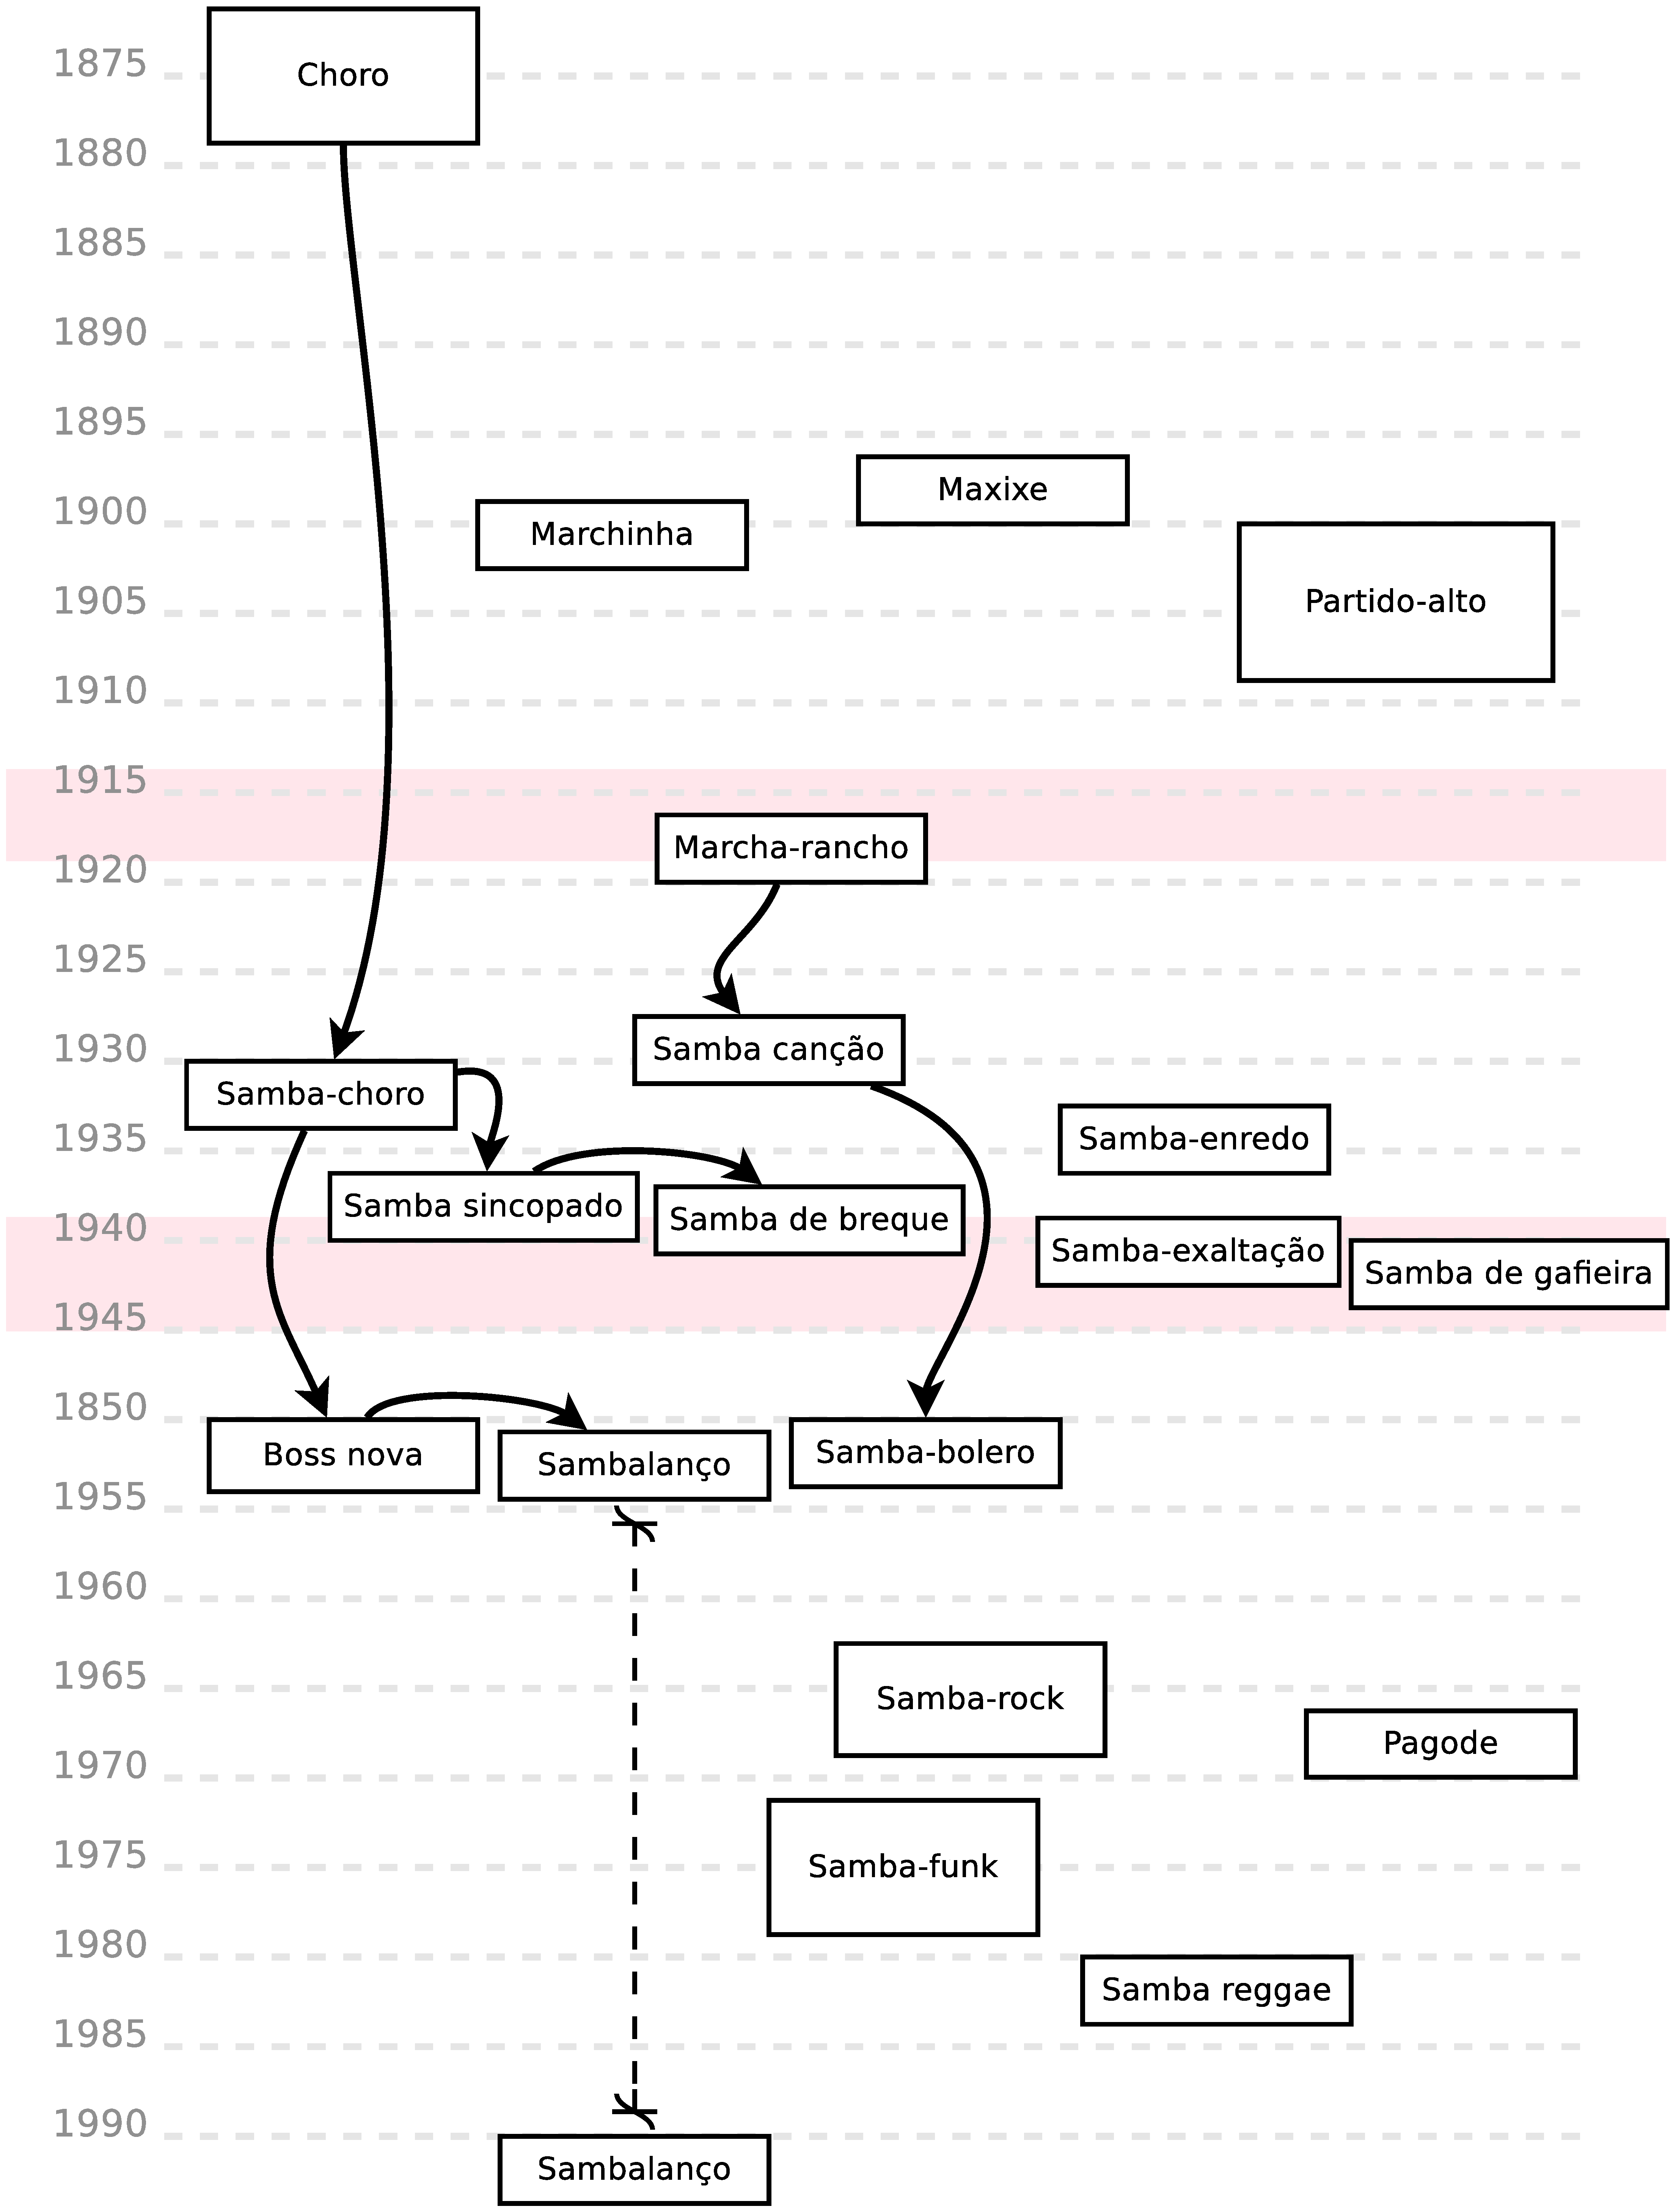
\includegraphics[width=1.0\textwidth]{chapters/cap-historia-musicasamba/musicatimeline.eps}
  \caption{Relação temporal entre os inícios dos subgêneros do samba.}
\label{fig:sambamusicatimeline1}
\end{figure}




%%%%%%%%%%%%%%%%%%%%%%%%%%%%%%%%%%%%%%%%%%%%%%%%%%%%%%%%%%%%%%%%%%%%%%%%%%%%%%%%
%% CAPITULO
%%%%%%%%%%%%%%%%%%%%%%%%%%%%%%%%%%%%%%%%%%%%%%%%%%%%%%%%%%%%%%%%%%%%%%%%%%%%%%%%
\chapterimage{chapter_head_2.pdf} % Chapter heading image

\chapter{Historia do samba de gafieira  (dança)}
\label{cap:sambagafieira}
\index{Dança!Samba de gafieira}


\section{Lundum (a dança do lundu)} 
\label{sec:lundu}
\index{Dança!Lundu}
O lundum é o estilo de dança que lhe corresponde ao gênero musical lundu \cite[pp. 18]{perna2002samba}.
Esta é uma dança, brasileira, de roda e umbigada; e teve sua origem no batuque dos bantos africanos,
e provavelmente foi trazida de Angola pelos escravos na segunda metade do século XVIII 
\cite[pp. 48]{tinhorao1986pequena} \cite[pp. 188]{dourado2004dicionario},
sendo que as primeiras referencias conhecidas se remontam a 1780 
descrevendo a dança como indecente e licenciosa \cite[pp. 51]{tinhorao1986pequena} \cite[pp. 19]{perna2002samba}.
Posteriormente foi introduzida aos salões das cortes do Brasil e Portugal, 
dançado elegantemente nas cortes, porem indecentemente pela gente comum   
\cite[pp. 19]{perna2002samba} \cite[pp. 188]{dourado2004dicionario}.
No Brasil esta dança teve influencias da ``Modinha''(Portuguesa) e do ``Fandango''(Espanhol) \cite[pp. 188]{dourado2004dicionario}.

A partir de 1820 o lundum é apresentado, como dança de caráter libidinoso nos teatros de Baia, Pernambuco e Rio de Janeiro;
onde eram representados pequenos quadros cômicos, 
mostrando a umbigada e outras caraterísticas da dança \cite[pp. 19]{perna2002samba}.


\section{Maxixe (dança)}
\label{sec:maxixe}
\index{Dança!Maxixe}
Esta é uma dança urbana afro-brasileira \cite[pp. 4]{musicasambavariasdef1}, 
em compasso binário, surgida em Rio de Janeiro, 
nos forrós da Cidade Nova e nos cabarés de Lapa \cite[pp. 465]{marcondes1977enciclopedia}  \cite[pp. 198]{dourado2004dicionario}, 
aproximadamente entre 1870 e 1880 
\cite[pp. 58]{tinhorao1986pequena} \cite[pp. 465]{marcondes1977enciclopedia}  \cite[pp. 62]{reinato2010musica},
estendendo-se  aos clubes carnavalescos e aos palcos dos teatros de revistas \cite[pp. 465]{marcondes1977enciclopedia}.

A sociedade local considerava ao maxixe como uma dança de baixe ralé, 
pois era entendida como um modismo indecente das classes baixas, tão imoral quanto o Lundum \cite[pp. 198]{dourado2004dicionario}.
Num principio o maxixe (dança) não tinha música própria e era dançado de forma livre nas músicas de 
tango, havanera, polca, schottisch, mazurca e lundu 
\cite[pp. 465]{marcondes1977enciclopedia} \cite[pp. 58]{tinhorao1986pequena}  
\cite[pp. 198]{dourado2004dicionario} \cite[pp. 62]{reinato2010musica}; 
e só foi ate o final do século XIX que ganhou uma música com gênero próprio \cite[pp. 465]{marcondes1977enciclopedia},
para mais detalhes do maxixe (música) ver a Seção \ref{subsec:maxixe}.

Uma explicação muito interessante sobre como se dança o maxixe é cantado pela atriz Aurélia Delorme,
numa representação num quadro de revista, interpretando o ``Maxixe Aristocrático'' (composto por José Nunes em 1904), 
que arrancava aplausos e provocava pedidos de bis;
o seguinte texto indica sua pauta \cite[pp. 80-81]{efege1974maxixe} \cite{REIS2003}: 
\begin{citando}
O maxixe tem ciência,\\
ou pelo menos tem arte.\\
Para haver proficiência\\
basta mexer certa parte.\\
Pois o próprio Padre Santo,\\
sabendo o gosto que tem,\\
virá de Roma ao Brasil\\
dançar maxixe também.\\ 
\end{citando}


No início do século XX o maxixe (dança e música) foi exportado a Europa, atingindo um grande sucesso
\cite[pp. 465]{marcondes1977enciclopedia};
entre os primeiros brasileiros registrados como exportadores do maxixe, estão 
os ``Geraldos''; par de dançarinos formado por Geraldo Magalhães e Antonina,
 que a finais de 1908 fizeram uma turnê por Inglaterra, França, Espanha e Portugal,
como consta no jornal ``Gazeta de notícias'' do 31 de Janeiro de 1909 
\cite[pp. 3]{maxixegeraldos} \cite[pp. 79, 93]{tinhorao1986pequena}.
Porem, antes da chegada dos ``Geraldos'', o maxixe como música e dança, já tinha sido
apresentado à sociedade europeia através da novidade dos discos; por exemplo,
no 29 de maio de 1905, no jornal ``La liberte'' de Paris, se menciona uma representação de maxixe no Olympia,
apresentado por Gaby Deslys\footnote{Que logo seria parceira de dança de Duque.} e 
os senhores Berthez e Rosario la Zingara \cite[pp. 3]{maxixe1905}.
Nesse mesmo ano, o compositor francês Charles Borel-Clerc criou um maxixe titulado ``la matchiche'',
música que alcançou sucesso\footnote{Aconselho procurar a música porque é gostosinha de ouvir, 
e tenho a impressão de ter escutado ela antes, em algum filme de faroeste sendo interpretado por algum pianista numa taberna.} 
em Europa e no Brasil \cite[pp. 79]{tinhorao1986pequena} \cite[pp. 175]{delfino1998brasil} \cite[pp. 180]{dourado2004dicionario};
e em 1906 uma dupla de dançarinas francesas, Rieuse e Nichette, 
apresentou o maxixe no Teatro Marigny, nos Champs-Élysées \cite[pp. 79-80]{tinhorao1986pequena}.

%% Pag 71-79 %% https://books.google.com.br/books?id=ONI9DwAAQBAJ&dq=maxixe+%2B+duque+%2B+gaby&hl=pt-BR&source=gbs_navlinks_s
%% Pag 181, referencia 14 %% https://books.google.com.br/books?id=ONI9DwAAQBAJ&dq=maxixe+%2B+duque+%2B+gaby&hl=pt-BR&source=gbs_navlinks_s

Nos casos anteriores, o maxixe era dançado de forma espontânea e não padronizada;
porem nesses anos surgiu
o disciplinador do maxixe, este foi um baiano dentista e dançarino, 
chamado Antônio Lopes de Amorim Diniz (1884-1953), também conhecido como ``Duque'', 
que antes do seus 25 anos, 
aproximadamente entre 1905 e 1908\footnote{Numa 
entrevista em setembro de 1915, na sua chegada ao Brasil \cite[pp. 1]{maxixeparis1915:0}, 
Duque indica que esteve 14 anos longe da Bahia e 10 anos fora do Brasil;
sobre este último dado, ao ser um número redondo, 
pode indicar uma forma rápida e coloquial de falar: 
 10, 9, 8 ou 7 anos, indicados em ordem que diminui a probabilidade.
Isto coincide com o que menciona Marcondes no seu livro 
``Enciclopédia da música brasileira: erudita, folclórica, popular'',
quando menciona que foi em 1909 que Duque chega a Paris \cite[pp. 242]{marcondes1977enciclopedia}.} 
\cite[pp. 1]{maxixeparis1915:0} \cite[pp. 130]{efege1974maxixe} \cite[pp. 82-83]{tinhorao1986pequena} \cite[pp. 242]{marcondes1977enciclopedia},
partiu a Paris por motivos de trabalho\footnote{Perdeu 
todo o seu dinheiro no jogo e partiu a Paris representando 
um produto farmacêutico \cite[pp. 82]{tinhorao1986pequena}.}, e apos o fracasso deste empreendimento,
decide abrir uma escola de dança no número 5 da Cité Piagalle, em Paris, onde ensina um maxixe carioca estilizado,
com o nome ``le vrai tango brésilien''; em pouco tempo, 
Duque virou muito cobiçado como professor e companheiro de dança,
fazendo parcerias com grandes vedetes da época \cite[pp. 82]{tinhorao1986pequena} \cite[pp. 131]{efege1974maxixe}; 
por exemplo; seguindo Tinhorão \cite[pp. 82]{tinhorao1986pequena} 
existe uma crônica escrita por Gaston Deval em 1909 e uma menção na revista Chiffon,
que elogiavam uma dança que Duque e Mlle Arlette Dorgère realizaram no Trocadéro;
%% Dorgère https://gallica.bnf.fr/ark:/12148/bpt6k6537821b/f17.item
novamente, seguindo Tinhorão, a referida página da revista Chiffon pode ser achada
reproduzida num artigo de Brício de Abreu chamado 
``Propaganda de nossa música popular -- Duque -- historia do maxixe na Europa'',
localizado\footnote{Não tenho achado referencias online a nenhum desses documentos.} 
no acervo no Serviço Nacional de Teatro ou 
no número 7/8 da revista  Música \& Disco (1960) \cite[pp. 94]{tinhorao1986pequena}.
%por exemplo, Duque dança em julho e setembro de 1909 com a dançarina grega Crysis, no Chez Ciro's e no Magic City, respetivamente \cite[pp. 82]{tinhorao1986pequena} \cite[pp. 131]{efege1974maxixe};

Porem, o trabalho de um praticante de dança a dois é incompleto sem um par
que lhe ajude a polir sua arte,
e fora de parcerias espontâneas, Duque teve principalmente duas companheiras de dança.
\begin{description}

% retrato maria lino http://memoria.bn.br/DocReader/030015_02/18912
\item[1909:] Maria Lina chega a França \cite[pp. 3]{maxixe1913marialina},
pois ela comenta que chegou a Paris dois anos apos iniciada sua gira no Brasil em 1907,
isto coincide com os dados encontrados nos jornais do Brasil, 
onde sua última menção antes do retorno da Europa,
é no dia 27 de janeiro de 1909 no jornal ``O Rio-Nú'' (RJ) \cite[pp. 3]{maxixe1909maria}.
Maria é nascida na Itália em 1880, porem aos quatorze anos, foi ao Brasil \cite[pp. 63]{efege1974maxixe}.



\item[1912:] Duque é mencionado como o ``roi du tango'' (rei do tango)
por muitos jornais da época; por exemplo,
no dia 8 de agosto de 1912, no jornal ``Comoedia'' (Paris) \cite[pp. 3]{maxixe1913reidotango:0:b},
no dia 8 de março de 1913, no jornal ``Le Matin'' (Paris) \cite[pp. 4]{maxixe1913reidotango:0},
no dia 16 de março de 1913, no jornal ``L'Intransigeant'' (Paris)  \cite[pp. 3]{maxixe1913reidotango:1},
no dia 20 de março de 1913, no ``Le Journal'' (Paris) \cite[pp. 7]{maxixe1913reidotango:2}, 
etc.
%\item[1913 (fevereiro):] Maria lina dança maxixe sozinha nume festa sem Duque, se conhecerão depois? %% https://gallica.bnf.fr/ark:/12148/bpt6k46019546/f9.item


\item[1913 (março):] No dia 7 março, seguindo o ``Le Journal'',  Duque e Maria lina\footnote{No dia 7 março
no ``Le Journal'' chamam a Maria Lina como ``Maria Line'';
no Brasil, antes de sua chegada a França vários jornais chamam ela de Maia Lino,
porem a partir de 1913 os jornais geralmente chamam ela de ``Maria Lina''.} 
iniciam a interpretar a opereta ``la Reine s'amuse'',
na sala de espetáculos musicais de Paris ``l'Olympia'' \cite[pp. 8]{maxixe1913reidotango:0:a};
porem, em entrevista, Maria Lina indica que foi o dia 4 de março \cite[pp. 3]{maxixe1913marialina};
os dias seguintes à estreia, muitos jornais, como ``Le Matin'',
falam do grande sucesso da apresentação \cite[pp. 4]{maxixe1913reidotango:0},
fenômeno que se repete pelo menos em todo esse mês de apresentações 
\cite[pp. 4]{maxixe1913reidotango:0} \cite[pp. 3]{maxixe1913reidotango:1} \cite[pp. 7]{maxixe1913reidotango:2}.
Seguindo o mencionado por Maria Lina numa entrevista realizada quando volta ao Brasil,
4 anos apos sua chegada a Paris, 1913, 
ela e Duque se lançaram aos principais centros de diversões, dançando maxixe \cite[pp. 3]{maxixe1913marialina}.


É interessante ressaltar que no dia 20 de março no ``Le Journal'' (Paris), existe uma publicidade 
para a venta de um livreto de partituras musicais que usa o nome de Duque (garoto propaganda),
chamado ``Duquinho'', que são tangos brasileiros dançados por Duque e Maria Lina no Olympia,
enviado por 2 francos em contra reembolso postal dirigido ao editor M. Sarrablo \cite[pp. 7]{maxixe1913reidotango:2}.
%% DUQUINHO: https://www.ernestonazareth150anos.com.br/posts/index/23

\item[191X:] Duque e Maria lina estiveram durante mês e meio no Hipódromo de Londres,
e também em diversos ``music-halls'' da cidade
\cite[pp. 3]{maxixe1913marialina} \cite[pp. 83]{tinhorao1986pequena} \cite[pp. 1]{maxixeparis1915:0}.

\item[191Y:] Duque e Maria Lina  ganham um concurso de dança no Admirals Palast em Berlim,
como declara Maria Lina, sem indicar data \cite[pp. 3]{maxixe1913marialina} \cite[pp. 83]{tinhorao1986pequena}.

\item[1913 (antes de agosto):] Maria lina volta ao Brasil,
e indica que trabalhou com Duque em Paris, Londres e Berlin \cite[pp. 3]{maxixe1913marialina}.

\item[1913 (outubro):] Duque e Gaby Delsys debutam no ``Théâtre-Imperial''
no dia 22 de outubro \cite[pp. 5]{maxixe1913duquegaby:3}.
 
%% Nome Gaby Deslys \cite[pp. 1]{maxixeparis1915:0}

%\item[191X:] Duque conhece a sua parceira definitiva, a dançarina francesa e manequim, Gaby Deslys \cite[pp. 84]{tinhorao1986pequena}.
%\item[1912:] A popularidade da dupla Duque e Gaby desponta \cite[pp. 84]{tinhorao1986pequena}.


\item[1913 (dezembro 6):] Duque e Gaby Deslys dançam na
inauguração do Dancing Palace, no Luna Park do Paris 
\cite[pp. 14]{maxixeparis1914} \cite{maxixe1913dancingpalace:1}, 
ante a presença do Rei Jorge V (da Inglaterra) e 
do presidente da republica de França  Raymond Poincaré\footnote{Tinhorão,
indica erroneamente que foi ante o matemático (Henri) Poincaré,
porém isto é impossível pois este morreu em 1912  \cite[pp. 84]{tinhorao1986pequena}}, 
\cite[pp. 73]{shaw2018tropical}.
Apos a apresentação, Duque toma o cargo do diretor artístico do Dancing Palace no Luna Park \cite[pp. 4]{maxixe1913dancingpalace:2}.
%\item[1913:], Duque e Gaby dançam para o Papa Pio X, em Roma; dança que gostou muito a pontífice, apontando ele que na sua juventude ele executava um estilo de dança com um ritmo quase tão vivo quanto o ``tango brasileiro''  \cite[pp. 84]{tinhorao1986pequena}.

\item[1914-1915:] O 22 de agosto de 1914, Duque e Gaby 
partem para Lisboa\footnote{Em Portugal Duque e Gaby sofrem um grande prejuízo em bens materiais, 
no incêndio do Teatro da Republica (Lisboa), acontecido em setembro \cite[pp. 4]{maxixe1914duque:1}.}
 para fazer apresentações, 
e desde ali a Estados Unidos onde dançam em New York
por 5 messes\footnote{No 
dia 20 de Fevereiro de 1915 a revista Fon Fon menciona o grande sucesso de Duque em New York \cite[pp. 45]{maxixe1915duqueEEUU:1}.}, 
em vários teatros da cidade; 
dos estados unidos foram para Havana e acabando seu contrato lá  
se dirigiram finalmente ao Brasil \cite[pp. 6]{maxixe1916duquegaby:1} \cite[pp. 1]{maxixeparis1915:0}.

\item[1915 (setembro):] Duque e Gaby chegam ao Brasil, 
sendo calorosamente recebidos em Rio de Janeiro por amigos e admiradores 
\cite[pp. 1]{maxixeparis1915:0} \cite[pp. 2]{maxixeparis1915}  \cite[pp. 73-75]{shaw2018tropical},
foi nesta época que o maxixe foi reintroduzido ao Brasil, com o nome higienizado branqueado de 
``tango brasileiro'' ou ``maxixe de salão'' \cite[pp. 74-75]{shaw2018tropical}.

\item[1915-1916 (janeiro):] Duque e Gaby fazem uma gira em América do sul, 
trabalhando em Rio de Janeiro, São Paulo, Recife, Bahia, Vitoria, Buenos Aires e Montevideo
\cite[pp. 6]{maxixe1916duquegaby:1} \cite[pp. 5]{maxixe1916duquegaby:2}. 
%\item[1916 (Janeiro):] Duque e Gaby viajam a Buenos aires, Argentina; para atuar no Teatro Nuevo \cite[pp. 76]{shaw2018tropical}.
%\item[1921 (Janeiro):] Duque volta a Paris \cite[pp. 78]{shaw2018tropical}.
\item[1916 - (adiante)  :] Etc.
\end{description}
%apresentando-se em Paris (1914) e em Londres (1922)  \cite[pp. 465]{marcondes1977enciclopedia};

Duque é considerado o civilizador do maxixe \cite[pp. 129]{efege1974maxixe};
porém, também podem entrar nesta categoria suas parceiras mais recorrentes como Maria Lina e Gaby Delsys;
por exemplo, Maria Lina numa entrevista menciona \cite[pp. 3]{maxixe1913marialina}:
\begin{citando}%%
\textbf{Entrevistador:} Mas, como é que o maxixe, essencialmente plebea,
poude se elevar de modo a transformar-se em uma dansa elegante?\\
\textbf{Maria Lina:} Bem podeis comprender que não fui dansar nosso 
grosseiro maxixe de plebe,
as passes communs da nossa indole sensual desregrada ...
Procurei modificar, o quanto possivel,
a brutalidade de certos desleixos immoraes da nossa dansa 
e consegui elevar o maxixe,
de modo a ser aceito na sociedade de Paris como uma dansa 
verdadeiramente elegante e que veiu suplantar o tango argentino, 
que tanto sucesso fazia...
\end{citando}

O maxixe durante seu tempo de auge acumulou uma boa quantidade de passos de dança, 
alguns destes são listados a continuação: 
\begin{itemize} 
\item balão \cite[pp. 93]{efege1974maxixe} \cite[pp. 465]{marcondes1977enciclopedia}, 
\item balão apagado \cite[pp. 68]{efege1974maxixe} \cite[aproximadamente min. 11:35]{MaxixeDocumentario1},
\item balão caindo  \cite[pp. 129, 131]{efege1974maxixe} \cite[pp. 62]{tinhorao1986pequena},
\item carrapeta  \cite[pp. 465]{marcondes1977enciclopedia}, 
\item cobrinha \cite[pp. 62]{tinhorao1986pequena},
\item corta-capim \cite[pp. 465]{marcondes1977enciclopedia} \cite[pp. 62]{tinhorao1986pequena}, 
\item corta-jaca (The skating step) \cite[pp. 131]{efege1974maxixe} \cite[pp. 112]{castle1914modern},
\item janela  \cite[pp. 129]{efege1974maxixe},
\item jocotó \cite[pp. 83, 96, 173]{efege1974maxixe},
\item maxixe puladinho \cite[pp. 177]{1920revista},
\item parafuso  \cite[pp. 68, 93, 129]{efege1974maxixe} \cite[pp. 465]{marcondes1977enciclopedia} \cite[pp. 62]{tinhorao1986pequena}, 
\item saca-rolha \cite[pp. 465]{marcondes1977enciclopedia}, 
\item sino \cite[pp. 68]{efege1974maxixe}, 
\item urubu malandro \cite[pp. 131]{efege1974maxixe},

\item the back two step \cite[pp. 119]{castle1914modern},
\item the two step \cite[pp. 108]{castle1914modern},
\item les à-côte (simgle step) \cite[pp. 112]{castle1914modern},
\item etc. 
\end{itemize}

Autores estrangeiros também dedicaram paginas a escrever sobre o maxixe,
temos o caso dos dançarinos estadunidenses, Vernon e Irene Castle, 
que em 1914 lançaram seu livro Modern Dancing,
onde titulam o capítulo VI como: ``The tango brésilienne, 
or maxixe -- The two step -- Les à-côte -- The skating step'' \cite[pp. 107]{castle1914modern},
e indicam que ``o tango e o maxixe são as danças do amanha'' \cite[pp. 85]{castle1914modern}.
Também temos o caso de Paul Boucher e Paul Gaffet que em 1928
publicam a segunda edição do livro de dança: 
``Toutes les Danses Pour Tous - Illustrées par la Photographie'',
onde ensinam samba além do maxixe (Ver Figura \ref{fig:LivroPaulBoucher}) \cite[pp. 14779]{library1929catalog}. 

  \begin{figure}[h!]
    \centering
    \ifx\EnableGrayScale\undefined
    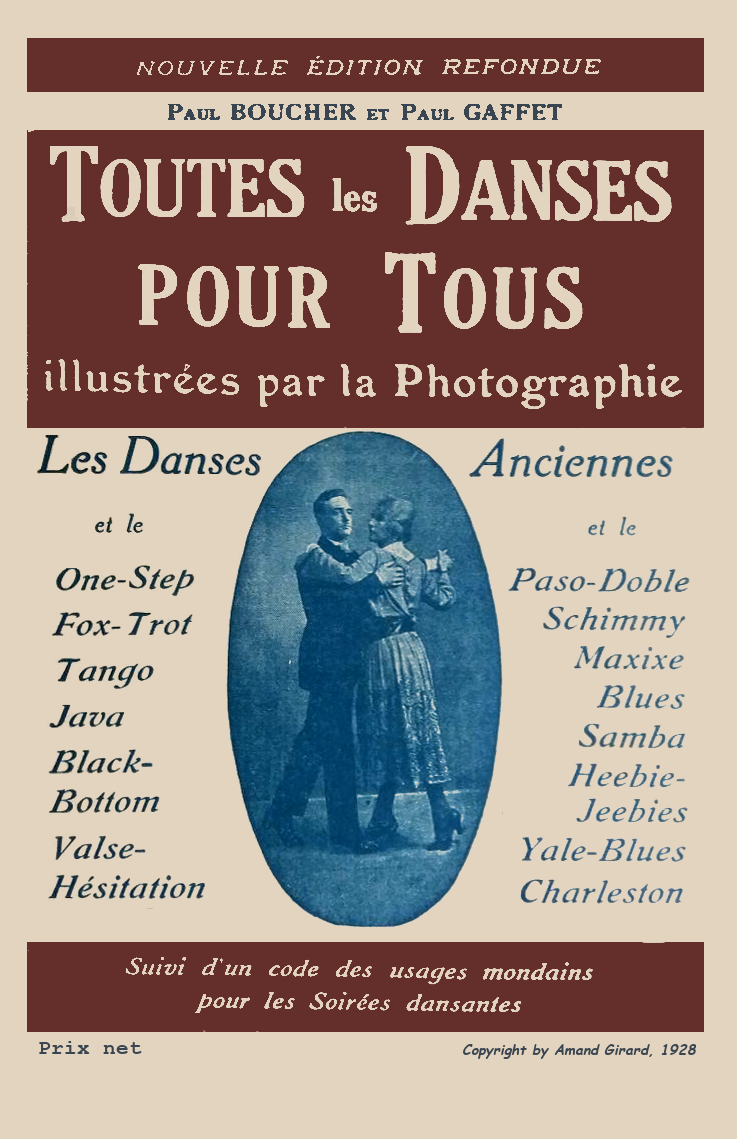
\includegraphics[width=0.5\textwidth]{chapters/cap-historia-sambagafieira/Toutes-les-danses-pour-tous.png}
    \else
    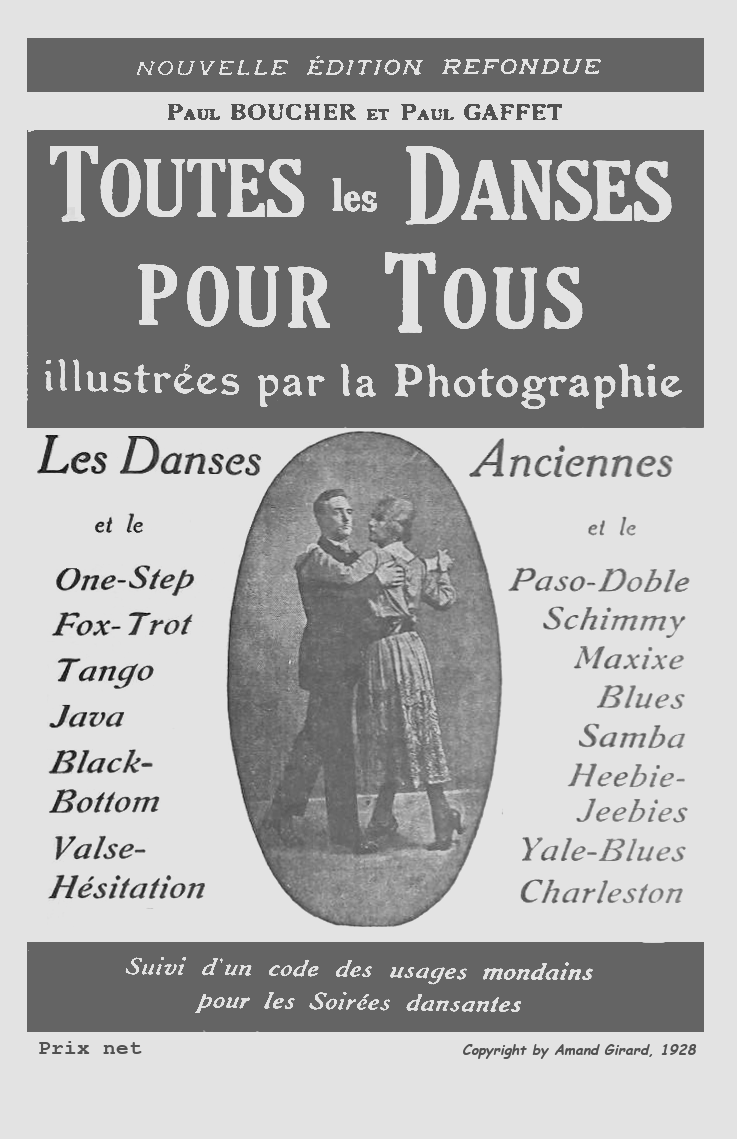
\includegraphics[width=0.5\textwidth]{chapters/cap-historia-sambagafieira/Toutes-les-danses-pour-tous-HSV.png}
    \fi
    \caption{Capa do livro ``Toutes les Danses Pour Tous - Illustrées par la Photographie'' (1928).}
    \label{fig:LivroPaulBoucher}
  \end{figure}


%%%%%%%%%%%%%%%%%%%%%%%%%%%%%%%%%%%%%%%%%%%%%%%%%%%%%%%%%%%%%%%%%%%%%%%%%%%%%%%%
\subsection{O nascimento do samba internacional}


\begin{description}
\item[1922:] O 18 de novembro de 1921 Duque retorna ao Brasil depois de uma viagem a Paris 
para participar numa competência de dança \cite[pp. 465]{marcondes1977enciclopedia} \cite[pp. 3]{duque1921:a}.
Apos algumas coordenações,
o 29 de janeiro de 1922, Duque novamente viaja\footnote{Graças 
ao financiamento do milionário Armando Guinle \cite[pp. 465]{marcondes1977enciclopedia}.} 
 a Paris para divulgar durante seis meses\footnote{Desde 
12 de fevereiro ate agosto \cite{BASTOS2005}. \cite[pp. 5]{batutas1922:c}} 
o samba e outros ritmos brasileiros, 
junto com os ``Oito Batutas''\footnote{O 
grupo estava dirigido por Pixinguinha e incluía Donga \cite{BASTOS2005}.} 
contratados por ele para esse fim
\cite[pp. 13]{duque1922:a} \cite[pp. 465]{marcondes1977enciclopedia}.
Na França o grupo é rebatizado como ``Les Batutas''\footnote{Os 
``Oito Batutas'' foram reduzidos a sete músicos \cite{BASTOS2005}.},
e teve apresentações principalmente no Shéhérazade, 
baixo a direção de Duque \cite[pp. 465]{marcondes1977enciclopedia} \cite{BASTOS2005};
existem varias referencias a estas apresentações, nos jornais franceses, pelo menos desde fevereiro,
ate abril de 1922, elogiando e promovendo as apresentações 
\cite[pp. 5]{batutas1922:a} \cite[pp. 4]{batutas1922:b} \cite{batutas1922:d},
como por exemplo a mostrada na Figura \ref{fig:LesBatutas}.


  \begin{figure}[h!]
    \centering
    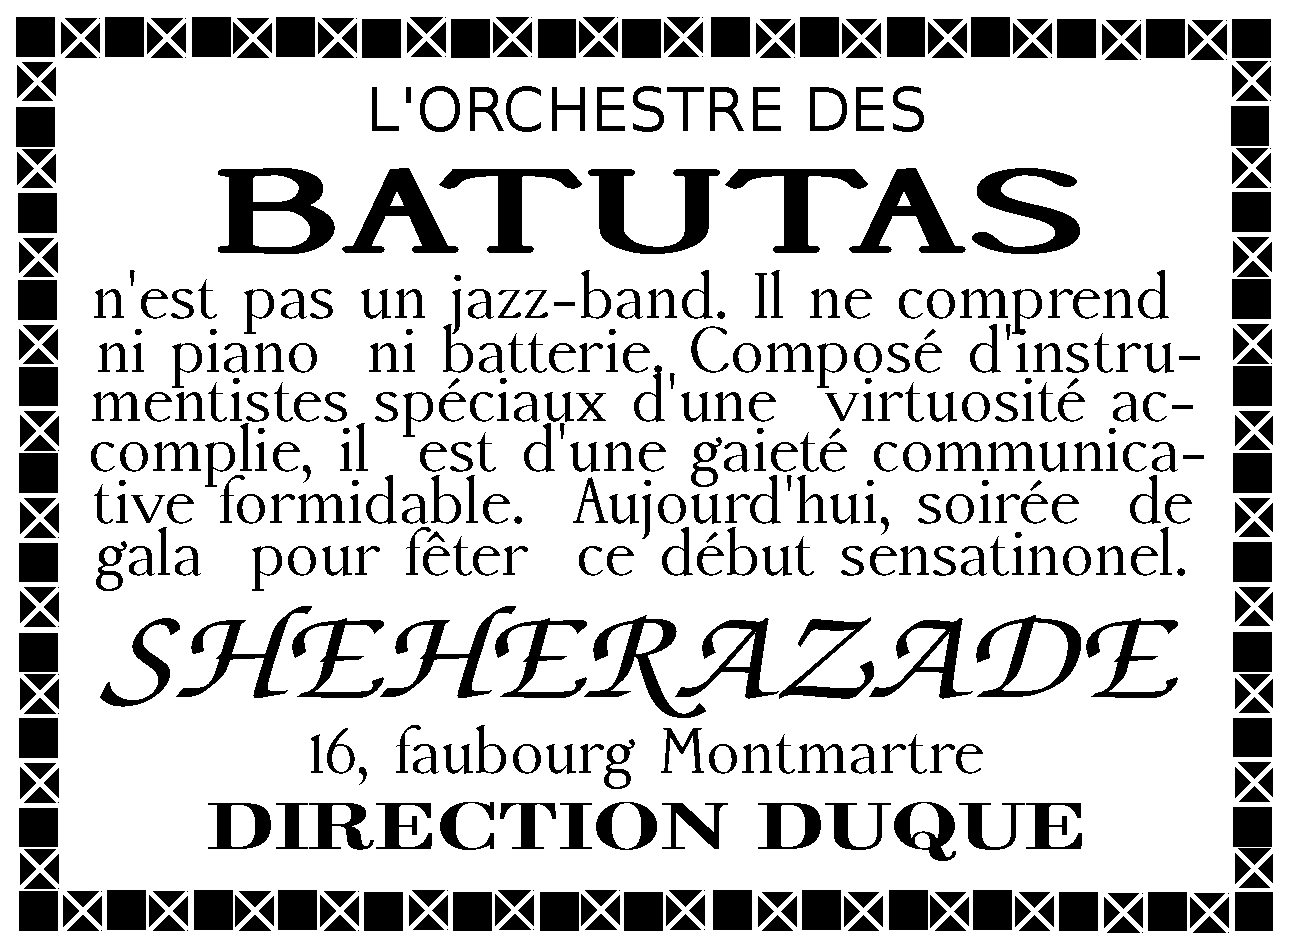
\includegraphics[width=0.5\textwidth]{chapters/cap-historia-sambagafieira/batutas.eps}
    \caption{Anuncio da orquestra dos ``Batutas'' no jornal ``Le Gaulois'' do dia 16 de fevereiro de 1922 \cite[pp. 4]{batutas1922:b}.}
    \label{fig:LesBatutas}
  \end{figure}

\item[1928:] Apos o trabalho feito em 1922 por Duque e os oito batutas, e o constante intercambio cultural entre Brasil e França, 
o samba ficou presente no consciente coletivo do povo parisiense.
No livro ``The Complete Book of Ballroom Dancing'' (1992) se menciona que foi ao redor de 1923
em França, que o ``samba de salão'' (a dança samba internacional) surge \cite[pp. 45]{stephenson1992complete},
como evidencia disto temos que em 1928, 
Paul Boucher e Paul Gaffet publicam  a segunda edição do seu livro de dança:
``Toutes les Danses Pour Tous - Illustrées par la Photographie'',
que inclui o samba além do já conhecidíssimo maxixe, ver Figura \ref{fig:LivroPaulBoucher}.

\item[1925-1929:] Nos Estados Unidos, seguindo o famoso músico brasileiro e líder de orquestra, 
Francisco Marti,
o samba substituiu ao maxixe ao redor de 1925 \cite[pp. 238]{hostetler1942walk}.
Por outro lado, seguindo o livro ``Social Dance: From Dance a While'' (1998),
o samba virou conhecido nos Estados Unidos ao redor de 1929
\cite[pp. 125]{harris1998social}.

\item[1933:] Nos Estados Unidos, o maxixe como expoente de cultura brasileira foi popular 
entre os dançarinos, aproximadamente desde\footnote{Em 
1915 os dançarinos Duque e Gaby fizeram apresentações em New York \cite[pp. 45]{maxixe1915duqueEEUU:1}.} 1910
ate 1920, e foi muito divulgado por Vernon e Irene Castle \cite[pp. 44]{stephenson1992complete}.
Porem, falando de pessoas fora do mundo da dança, 
foi em 1933 que o grande público conheceu o samba e a cultura brasileira no lançamento do filme
``Flying Down to Rio'',
onde Fred Astaire e Dolores del Rio dançam ``Carioca'' \cite[pp. 45]{maxixe1915duqueEEUU:1}.

\item[1938-1939:] Uma exibição de samba foi feita no novembro de 1938
para a ``New York Society of Teachers of Dancing''\footnote{1938, Sociedade de Professores de Dança de Nova York},
e para as pessoas em geral o interesse no samba seria ainda mais estimulado,
na ``Feira Mundial de Nova Iorque''\footnote{1939, World’s Fair in New York} (1939), 
onde o samba foi tocado no pavilhão brasileiro  \cite[pp. 45]{maxixe1915duqueEEUU:1}.

\item[1941:] Carmem Miranda divulgaria também o samba no
 filme de comédia musical ``That night in rio'' (1941) \cite[pp. 45]{maxixe1915duqueEEUU:1}.

\item[1944:] O filme musical ``Brazil'' (1944) é lançado em Hollywood,
onde o ``Soundtracks'' está a cargo do Ary Barroso;
isto apos o exito da música ``Brazil''\footnote{A 
música ``Brazil'' é na verdade ``Aquarela do Brasil'' (1939) 
\cite[pp. 73]{diniz2006almanaque} \cite[pp. 128]{perna2002samba} \cite[pp. 77]{fenerick2005nem}.} 
escrita por ele \cite[pp. 45]{maxixe1915duqueEEUU:1}.

\end{description}

Mais informação sobre o estilo de dança samba internacional, ver a Seção \ref{subsec:DancaSambaInternacional}.
%É criado o estilo de samba internacional \cite[pp. 78]{shaw2018tropical}.

%%%%%%%%%%%%%%%%%%%%%%%%%%%%%%%%%%%%%%%%%%%%%%%%%%%%%%%%%%%%%%%%%%%%%%%%%%%%%%%%
\section{Samba de gafieira (dança)}
\index{Dança!Samba de gafieira}
O samba de gafieira, como dança, descende principalmente do maxixe (dança),
que a sua vez foi gerado  pela união do  lundu, 
a polca e outras danças europeias.
Assim, misturando o maxixe com a ginga, e o ritmo de outras danças africanas, 
é que se obteve o samba dançado nas gafieiras \cite[pp. 139]{perna2002samba}, também chamado
samba de salão ou samba carioca \cite[pp. 50]{fornaciari1947aprender},
atualmente entenderíamos a este samba como o samba de gafieira primigênio\footnote{
Primitivo; primordial; o primeiro da sua espécie. = PRIMÍGENO \cite{priberamprimigenio}.
}.




A Figura \ref{fig:formuladosambagafieira} mostra a árvore genealógico do samba de gafieira,
visto quando o samba (música) fez sua aparição nos salões de dança denominados já no \AnoLivro~ como gafieiras.
\begin{figure}[h]
  \centering
  \begin{subfigure}[b]{0.52\textwidth}
    \centering
    \includegraphics[width=\textwidth]{chapters/cap-historia-sambagafieira/sambagafieiraformula.eps}
    \caption{Formação dos primeiros sambas dançados nas gafieiras ou samba de gafieira (primigênio).}
    \label{fig:formuladosambagafieira}
  \end{subfigure}
  ~~
  \begin{subfigure}[b]{0.37\textwidth}
    \centering
    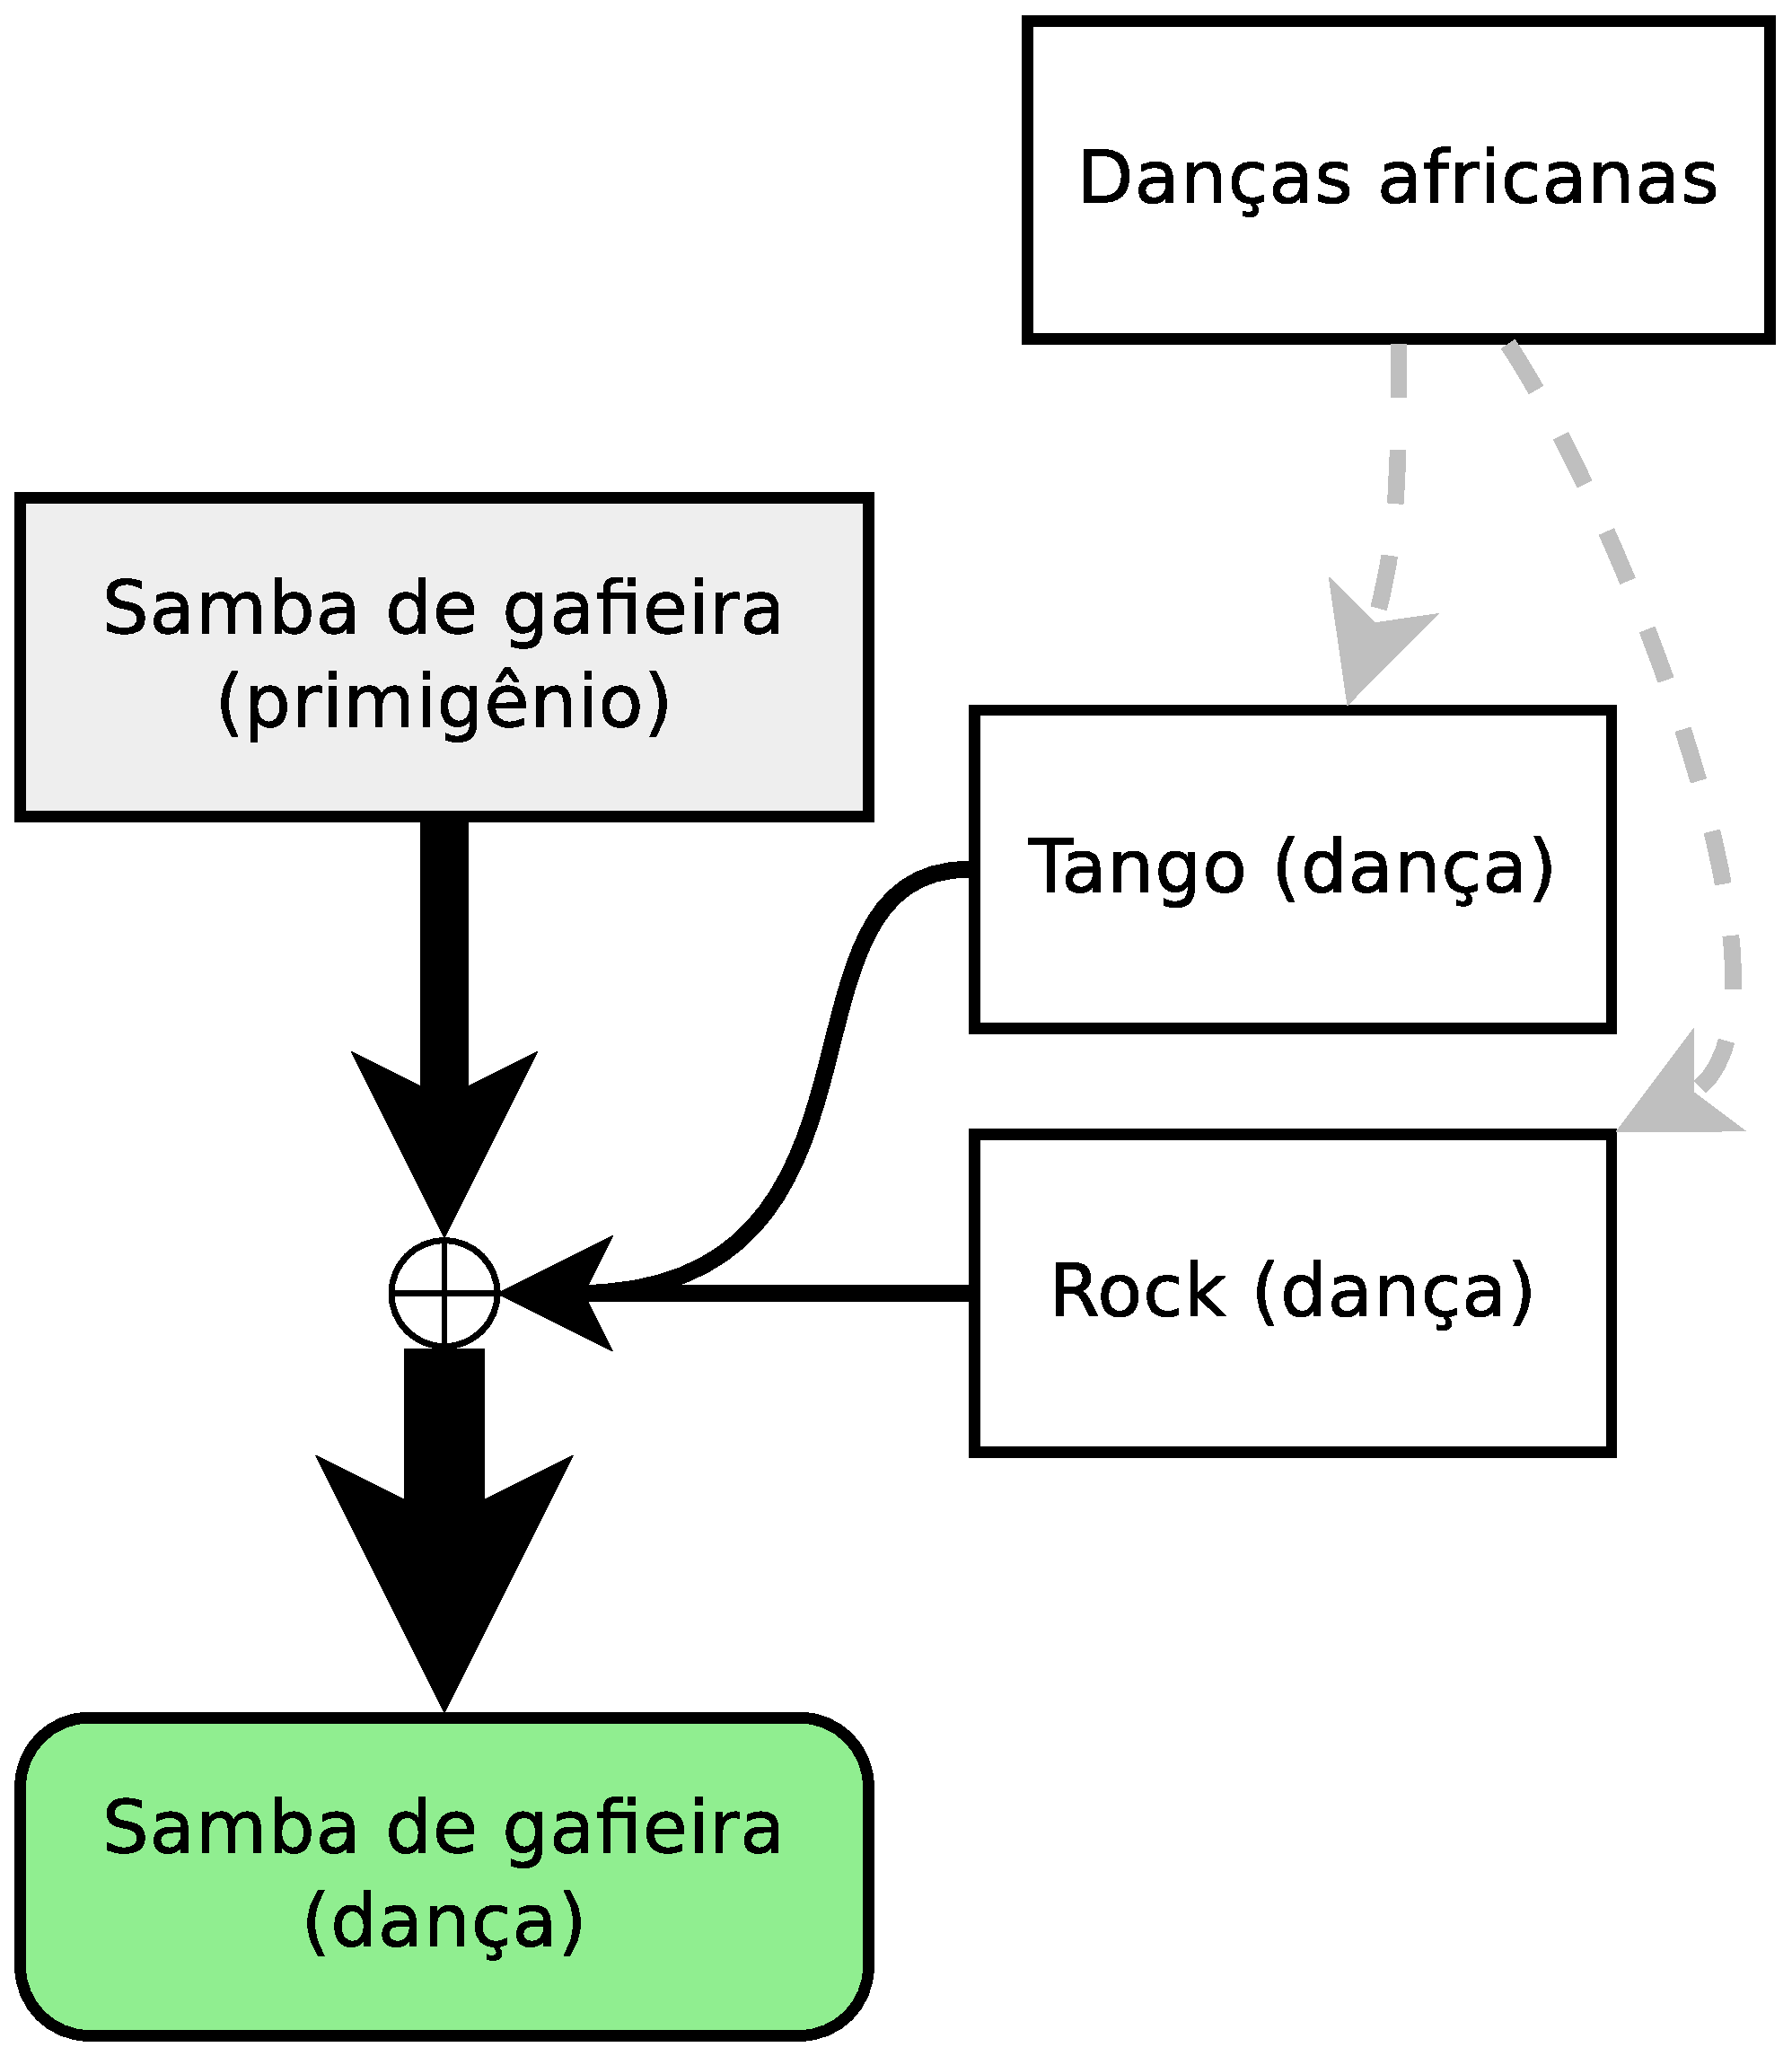
\includegraphics[width=\textwidth]{chapters/cap-historia-sambagafieira/sambagafieiraformula2.eps}
    \caption{Formação do samba de gafieira (atual).}
    \label{fig:formuladosambagafieira2}
  \end{subfigure}
\caption{Formula da criação do samba de gafieira.}
\label{fig:formuladosambagafieiraall}
\end{figure}


No janeiro de 1922, o professor de dança Duque junto com os ``Oito Batutas'', 
viaja a Paris para divulgar o samba e outros ritmos brasileiros
\cite[pp. 13]{duque1922:a} \cite[pp. 465]{marcondes1977enciclopedia},
pode-se deduzir que para esta época já existia algum tipo de forma de dançar o samba nos salões, 
pelo menos algum estilo próprio de Duque,
para ser apresentado na Europa. Isto é assim confirmado porque em 1928,
em Paris, se publicava a segunda edição do livro de dança de Paul Boucher e Paul Gaffet,
titulado
``Toutes les Danses Pour Tous - Illustrées par la Photographie'',
que incluia o samba além do já conhecidíssimo maxixe, ver Figura \ref{fig:LivroPaulBoucher}.


O aparecimento do samba nos salões de dança no Brasil, 
foi um grande impacto para as pessoas que frequentavam estes lugares;
sendo considerado um ritmo novo e ligeiro,
que desagradou aos bailarinos de maior idade e menos ágeis \cite[pp. 6 - cad. B]{entrevistajuliojournalbrasil1}.
O senhor, Júlio Simões, Administrador da ``Kananga do Japão'' e posteriormente socio
do ``Elite Club'', chegou a temer pelo futuro do seus empreendimentos; porem, para sorte dele, 
o samba fez muito sucesso no Elite,
e passou a ser considerado vestibular indispensável para qualquer pessoa que pretendesse ser bailarino, 
compositor ou instrumentista \cite[pp. 6 - cad. B]{entrevistajuliojournalbrasil1}.

Pode-se estabelecer o ingresso do samba aos salões de dança no Brasil numa época anterior e próxima da década de 1930,
dado que Júlio Simões, trabalhou na ``Kananga do Japão'' ate o ano de 1929 \cite[pp. 3 - cad. 3]{juliosimoes}  
\cite[pp. 11]{eliteinaugura} \cite[pp. 1 - cad. B]{gafieira2000reis}, pelo que sua preocupação sobre o samba 
nesse salão de dança deve ser anterior a essa data, porem não muito atrás dado que 
suas preocupações ainda eram vigentes na sua época no ``Elite Club'' 
que inciou em 1930 \cite[pp. 11]{eliteinaugura} \cite[pp. 3 - cad. 3]{juliosimoes} \cite[pp. 10]{simoesjournalbrasil1}.

\PRLsep{Os sambas nos salões em 1940}

O samba dançado nas gafieiras se firmou na década de 1940 \cite[pp. 142]{perna2002samba}. 
Em palavras do Prof. de dança Gino Fornaciari, 
a dança do samba praticada nos salões ou samba carioca (anterior a 1947 \cite[pp. 50]{fornaciari1947aprender}), 
 tinha um parecido com o Foxtrot e a Rumba, se dançava numa música sincopada com compasso binário,
sendo esta dança a preferida do mulato brasileiro
%sendo este estilo de dança de salão que nasceu na \hyperref[ref:batucadadanca]{\textbf{batucada}} 
%de pretos que descia à cidade na época das festas 
\cite[pp. 50-51]{fornaciari1947aprender}.


Na década de 1940 o samba dançado nos salões 
tinha 3 modalidades, samba-canção, samba-batucada e o samba liso \cite[pp. 58]{freitas1959danca} \cite[pp. 142-143]{perna2002samba} 
\cite[pp. 51]{fornaciari1947aprender}\cite[pp. 51]{fornaciari1950aprender}.\\
\begin{itemize}

\item \textbf{Samba-canção (dança):}
\index{Dança!Samba-canção} 

Este era uma dança com balanços aos lados que se executava de joelhos flexionados,
usando dois movimentos por cada compasso binario \cite[pp. 58]{freitas1959danca} 
\cite[pp. 51]{fornaciari1947aprender} \cite[pp. 143]{perna2002samba}; 
no ano 2001 se considera que este é um modo de dança extinto \cite[pp. 143]{perna2002samba}.

na Figura \ref{fig:samba-cancao-basico-frente} se mostra o passo básico para a frente do samba-canção,
e na  Figura \ref{fig:samba-cancao-basico-frente} o mesmo movimento para trás,
este eram usados antes de 1947 e inclusive no ano de 1959;
em ambos casos se usa os 2 movimentos antes mencionados, e a cor cinza indica a posição inicial \cite[pp. 51]{fornaciari1947aprender} \cite[pp. 59-60]{freitas1959danca}. 
\begin{figure}[h]
    \centering
    \begin{subfigure}[b]{0.4\textwidth}
        \centering
        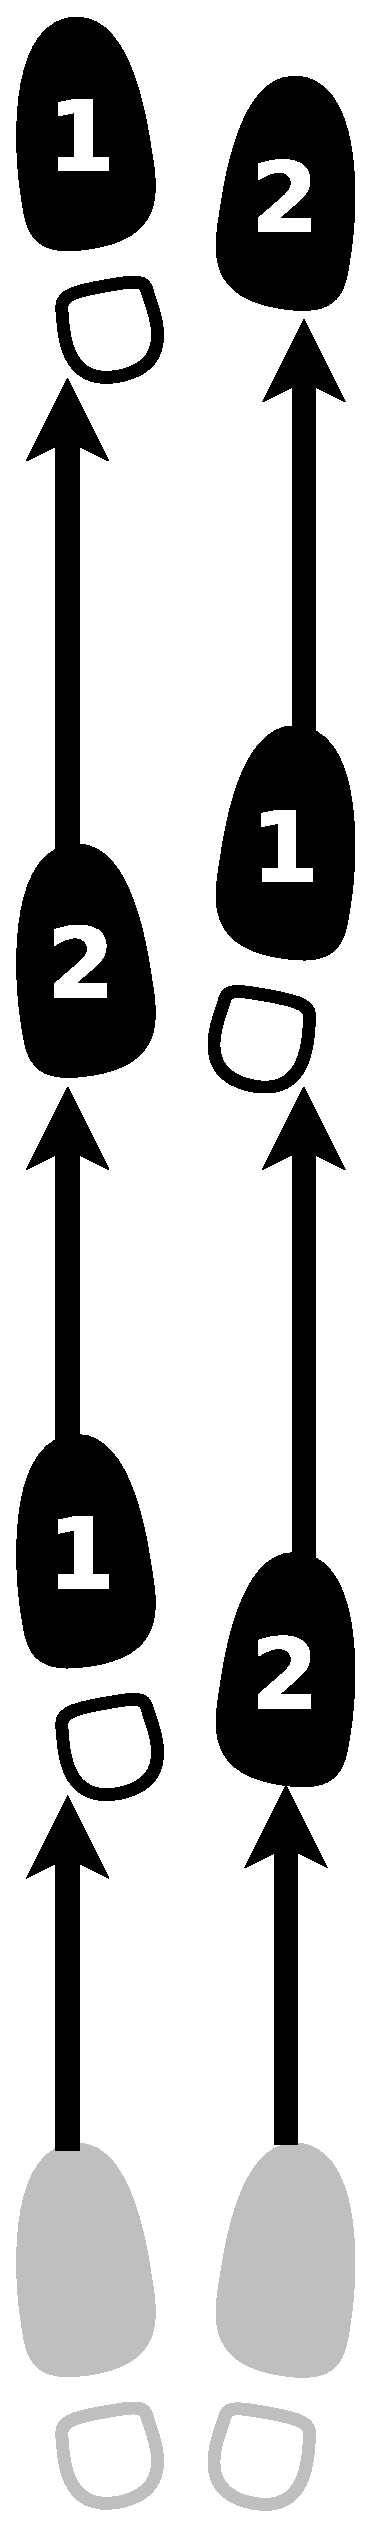
\includegraphics[width=0.25\textwidth]{chapters/cap-historia-sambagafieira/samba-cancao-basico-frente.eps}
        \caption{Passo básico para a frente.}
        \label{fig:samba-cancao-basico-frente}
    \end{subfigure}
    ~ %add desired spacing between images, e. g. ~, \quad, \qquad, \hfill etc. 
      %(or a blank line to force the subfigure onto a new line)
    \begin{subfigure}[b]{0.4\textwidth}
        \centering
	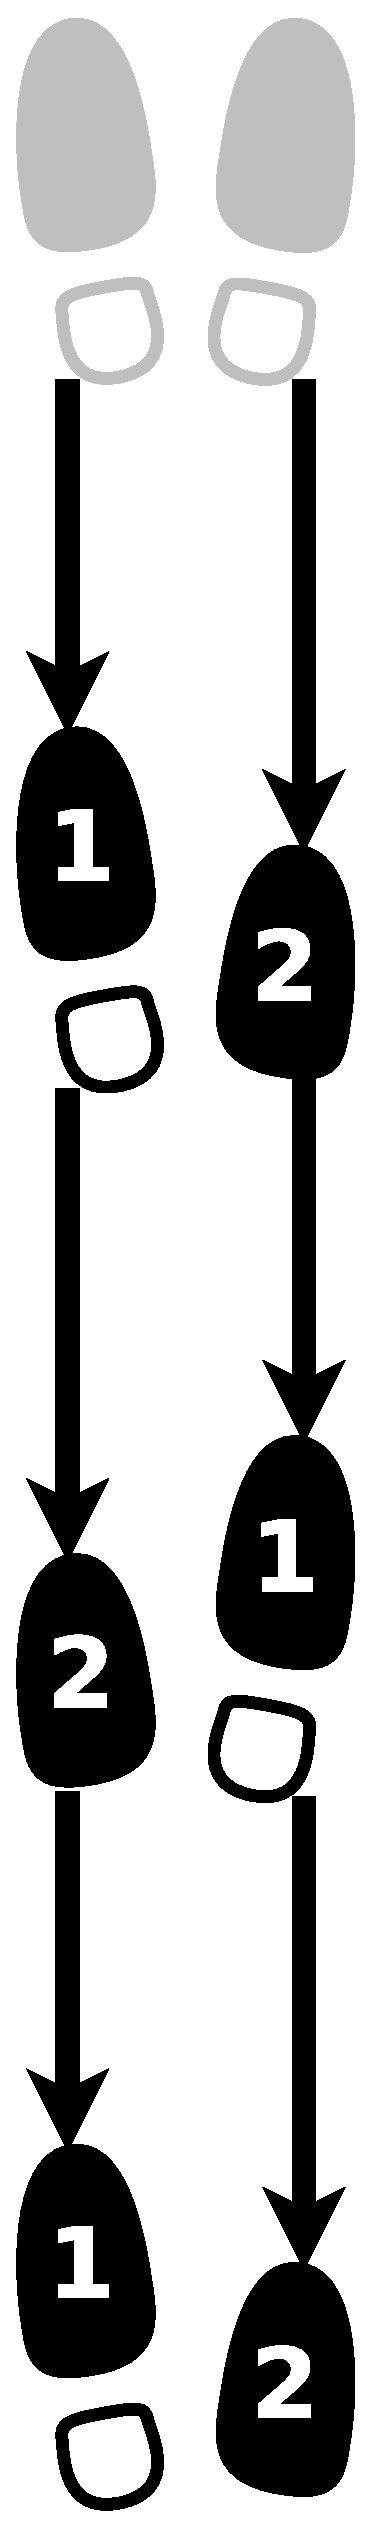
\includegraphics[width=0.25\textwidth]{chapters/cap-historia-sambagafieira/samba-cancao-basico-tras.eps}
        \caption{Passo básico para trás.}
        \label{fig:samba-cancao-basico-tras}
    \end{subfigure}
    \caption{Samba-canção da década de 1959.}\label{fig:samba-cancao-basico}
\end{figure}


\item \textbf{Samba-batucada:}
\index{Dança!Samba-batucada} 



Existe uma menção sobre este estilo no ``Jornal do Brasil'', no dia 9 de janeiro de 1938,
onde se indica \cite[pp. 4]{musicasambavariasdef1}:
\begin{citando}%%
Tentativas isoladas de puro 
snobismo e ás vezes de compreensão 
inexata da origem da 
musica e dansa, chamam-no de samba jongo, \textbf{samba batucada} ou
pretendem mistura-lo com o fox, -- samba fox ou com a rumba samba-rumba.
\end{citando}



No livro ``Feitiço decente: Transformações do samba no Rio de Janeiro (1917-1933)'' (2001),
se comenta, sobre uma roda do samba, que para o dançarino solista  escolher a seu sucessor podiam
existir duas modalidades, em ``samba liso'' (com umbigada) ou em ``samba duro'' 
(ou batucada) no qual a umbigada é substituída por uma pernada \cite[pp. 109]{sandroni2001feitico}.
Deste comentário pode ser deduzido de onde vem a denominação \textbf{samba-batucada}, 
que surgiu nos salões de dança apos 1930; pois já existia uma tradição na nomenclatura,
em separar duas formas de dançar uma mais leve (a liso) e uma mais brusca (batucada);
assim, a variante de samba no salão que tendia a explorar movimentos muito  gingados, bruscos ou rápidos,
foi nomeado de samba-batucada, em contraposição ao samba liso onde né se flexionavam os joelhos pra dançar.  



Seguindo o que indicam  os professores de dança Gino Fornaciari e Ivan Freitas,
nos seus respetivos livros, o samba-batucada era desde antes de 1947 e inclusive ate 1959, 
uma dança com balanços que se executava de joelhos flexionados  
e usava 3 movimentos por compasso, que exigia uma maior rapidez, 
especialmente no terceiro movimento que é mais rápido e curto 
\cite[pp. 61]{fornaciari1947aprender} \cite[pp. 58,66]{freitas1959danca};
seguindo essa descrição, 
o mais provável é que o samba-batucada se dançara seguindo uma distribuição de tempos,
muito parecida ao ritmo do baião de 1949 \cite{CORTES2014}, 
como pode-se ver na Figura \ref{time:sambabatucada};
nela se exemplifica a distribuição de tempos em relação ao uso dos pés;
onde na segunda pisada de cada compasso só se usa meia ponta do pé.
\begin{figure}[H]
\centering
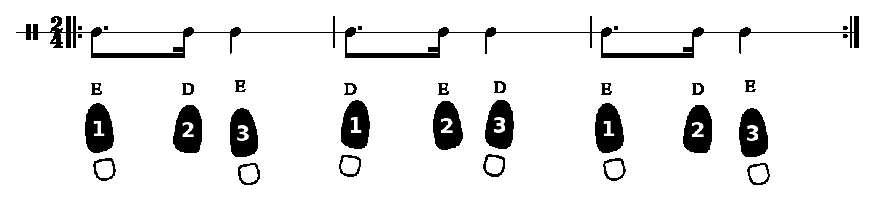
\includegraphics[width=\textwidth]{chapters/cap-historia-sambagafieira/sambabatucada.eps}
\caption{Ritmo das pisadas no samba-batucada.}
\label{time:sambabatucada}
\end{figure}
A descrição do movimento, que indica que a terceira pisada é mais rápida,
é um pouco ambígua, 
pois não se sabe se se refere à velocidade com a que o pé se desloca ate tocar o chão e contar 3,
ou se se refere à velocidade do movimento, apos ter pisado 3, para dar o seguinte passo;
porem, 
independentemente da assinação de números escolhida, 
a Figura \ref{time:sambabatucada} exemplifica bem as proporções na distribuição de tempos 
indicada pelos professores Fornaciari e Freitas para o samba-batucada.
Esta afirmação é coerente com o achado em livros referentes ao $\ll$samba internacional$\gg$ 
dessa época e posteriores\footnote{Nas referencias bibliográficas tenho achado publicações desde 1945 ate 1998,
indicando uma distribuição de tempos para o samba internacional como a apresentada na Figura \ref{time:sambabatucada}
\cite[pp. 7,176]{wright1945dance} \cite[pp. 193]{white1953dancing} \cite[pp. 69]{stephenson1992complete} \cite[pp. 125]{harris1998social}.}
\cite[pp. 7,176]{wright1945dance} \cite[pp. 193]{white1953dancing} \cite[pp. 69]{stephenson1992complete} \cite[pp. 125]{harris1998social},
que indicam para o samba internacional a mesma distribuição de tempos que a mostrada na Figura \ref{time:sambabatucada};
assim podemos intuir que o samba-batucada ainda tinha essa caraterística comum com seu ``primo'' internacional.



Sobre os passos de samba-batucada usados desde antes de 1947: 
A Figura \ref{fig:samba-batucada-basico-frente}  mostra o passo básico para a 
frente, do samba-batucada, 
e na  Figura \ref{fig:samba-batucada-basico-tras} temos o mesmo movimento para trás;
em ambos casos se usam passos em grupos de 3; a cor cinza indica a posição inicial \cite[pp. 61-62]{fornaciari1947aprender} \cite[pp. 63]{freitas1959danca}. 
\begin{figure}[h]
    \centering
    \begin{subfigure}[b]{0.4\textwidth}
        \centering
        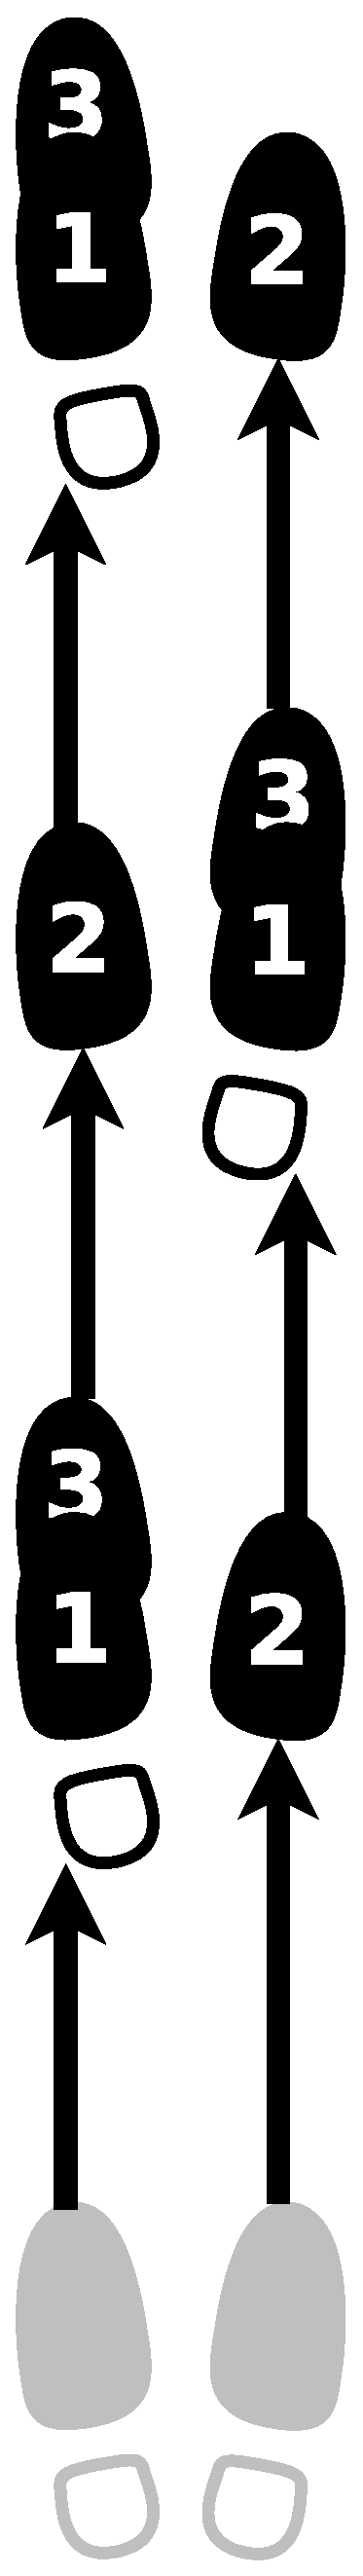
\includegraphics[width=0.25\textwidth]{chapters/cap-historia-sambagafieira/samba-batucada-basico-frente.eps}
        \caption{Passo básico para a frente.}
        \label{fig:samba-batucada-basico-frente}
    \end{subfigure}
    ~ %add desired spacing between images, e. g. ~, \quad, \qquad, \hfill etc. 
      %(or a blank line to force the subfigure onto a new line)
    \begin{subfigure}[b]{0.4\textwidth}
        \centering
	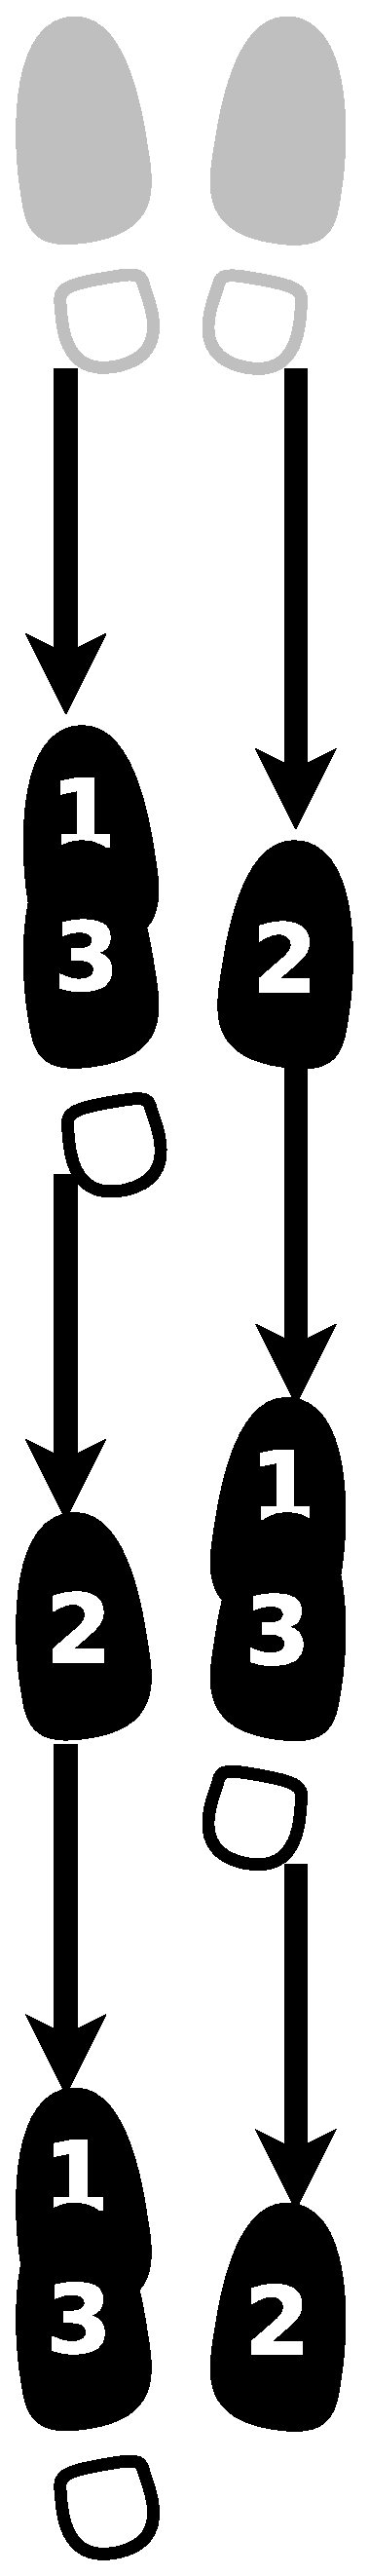
\includegraphics[width=0.25\textwidth]{chapters/cap-historia-sambagafieira/samba-batucada-basico-tras.eps}
        \caption{Passo básico para trás.}
        \label{fig:samba-batucada-basico-tras}
    \end{subfigure}
    \caption{Samba-batucada da década de 1959.}\label{fig:samba-batucada-basico}
\end{figure}

Outros passos conhecidos no ano de 1947, para este estilo de samba, tem nomes como: 
o pião, o balão, a cortada, a meia cortada, a joelhada, a patineta, e outros \cite[pp. 66]{fornaciari1947aprender}.
Para o Prof. Fornaciari, em São Paulo no ano de 1947 o pião e o balão são o mesmo movimento, 
sendo este o movimento mais importante do samba-batucada;
e a diferença do pião de \AnoLivro~ que se executa tradicionalmente em sentido horário,
o pião de 1947 se executava em sentido anti-horário \cite[pp. 68,72]{fornaciari1947aprender} 
\cite[pp. 73]{fornaciari1950aprender}.

Além dos estilos dançados nos salões, seguindo o Prof. Fornaciari, 
no ano de 1950 existem as danças estilizadas que estão orientadas 
para ser executadas em teatros \cite[pp. 149]{fornaciari1950aprender}. 
No caso do samba estilizado, este precisa de maior esforço físico dos dançarinos 
além de ser uma dança com maior flexibilidade, jogo de pernas, e com passos mais variados.
Por exemplo, no livro ``Como aprender a dançar'' (1950), temos um movimento que inicia com o condutor no abraço de dança,
e depois este dá uma patinada ou passo para atrás com a perna esquerda 
ao mesmo tempo que eleva ao seguidor \cite[pp. 160-1961]{fornaciari1950aprender};
este movimento  é muito similar a outro, chamado ``Elevador'', que é muito conhecido no samba de gafieira de \AnoLivro.
Nessa mesma página se explica outro movimento, esta vez chamado de ``cortada'', 
que não é outra coisa que uma pernada (presumivelmente só um contato leve) que o condutor da com sua perna esquerda,
sobre a perna direita do seguidor, um pouco abaixo do quadril\footnote{
Pessoalmente lembro ter visto este movimento ao contrario, quando um seguidor da esta pernada 
sobre a perna do condutor, um pouco abaixo do quadril, e o condutor aproveita para fazer uma sacada de perna,
inclusive tenho lembranças de telo visto no tango.}.
O livro também explica um movimento de samba estilizado chamado ``Joelhada'' \cite[pp. 160-1961]{fornaciari1950aprender}, 
que mas bem é uma postura, sendo esta muito similar à postura de ``Facão'' no samba de gafieira de \AnoLivro,
porem a postura do abraço é muito mais aberta, de modo que ao não estar colados,
o único ponto de contato entre os pares é a parte interna do joelho. 
Como uma semelhança mais com o facão,
no livro se indica que a joelhada pode ser executada apos o pião (do ano de 1947 que era em sentido anti-horário).
Outro movimento no samba estilizado é a ``calçada'', pela descrição feita no livro,
este movimento, é o que no samba de gafieira de \AnoLivro~ chamaríamos ou associaríamos com o ``Balão'' \cite[pp. 162]{fornaciari1950aprender},
com a diferença de que na versão explicada no livro, este movimento não termina numa ``cadeirinha'',
e simplesmente apos chegar ao lado da perna esquerda do condutor (que era quando acontecia a cadeirinha), 
o seguidor retorna ao lado direito do condutor. 

Finalmente o livro revela,
que o passo básico do samba estilizado é o passo básico do samba-batucada \cite[pp. 163]{fornaciari1950aprender},
assim, o termo samba estilizado indica uma versão melhorada do samba-batucada,
orientado para teatros e apresentações. Pela semelhança com os passos de samba de gafieira de \AnoLivro,
nos passos ``Elevador'', ``Balão'' e ``Facão'' podemos teorizar, de que a modalidade samba-batucada foi
a que finalmente se converteu ou aportou mais ao samba de gafieira atual.
Uma evidencia que sustenta esta ideia, a podemos encontrar no filme ``Aviso aos navegantes'' (1950) \cite[min. 40:35]{AtlantidaDance},
onde a partir do minuto 40:35 podemos ver uma apresentação de samba de salão (num teatro),
onde os dançarinos fazem os movimentos de elevador e balão, com uma sequencia de movimentos,
semelhante à descrita no livro ``Como aprender a dançar'' (1950) do Prof. Fornaciari.
Além de que em alguns momentos pode-se perceber movimentos de pés, 
com uma distribuição de tempos como na Figura \ref{time:sambabatucada},
dando maior força à hipótese de que essa era a distribuição de tempos para o samba-batucada nessa época. 
%O samba-batucada é o samba de gafieira (primigênio) \cite[pp. 143]{perna2002samba}.

\item \textbf{Samba liso:}
\index{Dança!Samba liso}

Era uma dança com balanços que se dançava sem flexionar os joelhos;
este é um estilo de dança que perdura ainda ate nossos 
dias \cite[pp. 58,62]{freitas1959danca} \cite[pp. 61]{fornaciari1950aprender} \cite[pp. 143]{perna2002samba}, 
para mais detalhes ver a Seção \ref{subsec:sambalisodef}.
\end{itemize}

\subsection{Evolução do samba nos salões}

Com o passar dos anos foram agregados elementos de outras danças a esse primitivo, samba de gafieira;
por exemplo, movimentos do tango e do rock \cite[pp. 142]{perna2002samba}, 
obtendo assim a forma de dança que vemos hoje em dia, ver Figura \ref{fig:formuladosambagafieira2}.

Asim, podemos falar do samba de gafieira como dança, só apos da aparição do samba nos
salões de dança abertos ao público, e a partir da criação do termo gafieira pra definir a estes lugares.
Com a mistura destes dois acontecimentos obtemos o termo, samba de gafieira,
que iniciou seu caminho na dança, mas como uma descrição do âmbito da dança (e da música), que como nome próprio.
Porem, a formação dos movimentos e corporalidade desta dança tem um caminho que data desde muito tempo atrás,
desde os batuques, dos morros e das rodas.


A primeira referencia achada\footnote{Que não quer dizer a primeira existente.} 
na ``Hemeroteca Digital Brasileira'' da Fundação Biblioteca Nacional,
foi na ``Revista da Semana''(RJ), no dia 25 de dezembro de 1948,
onde na seção ``Eros Volusia'', subseção ``O pitoresco da excursão'', se indica \cite[pp. 48]{sambagafieirarefbn}
\begin{citando}
Ensinando o samba aos ministros da República, 
fazendo o povo vibrar com o \textbf{samba de gafieira}, entusiasmando
o meio intelectual com seu francês muito doce,
contando coisas desconhecidas aos dançarinos francêses,
fazendo a dança brasileira figurar nos Archives Internationales de la Danse.
Eros Volusia satisfez o grande ideal de sua vida artística, sentindo-se contente
com o que realizou na França, embora a Europa não dê dinheiro a ninguém.
O lucro artístico é que compensa.
\end{citando}


A Figura \ref{fig:sambagafieiracrono} mostra a cronologia do uso do termo samba de gafieira. 

\begin{figure}[h]
  \centering
    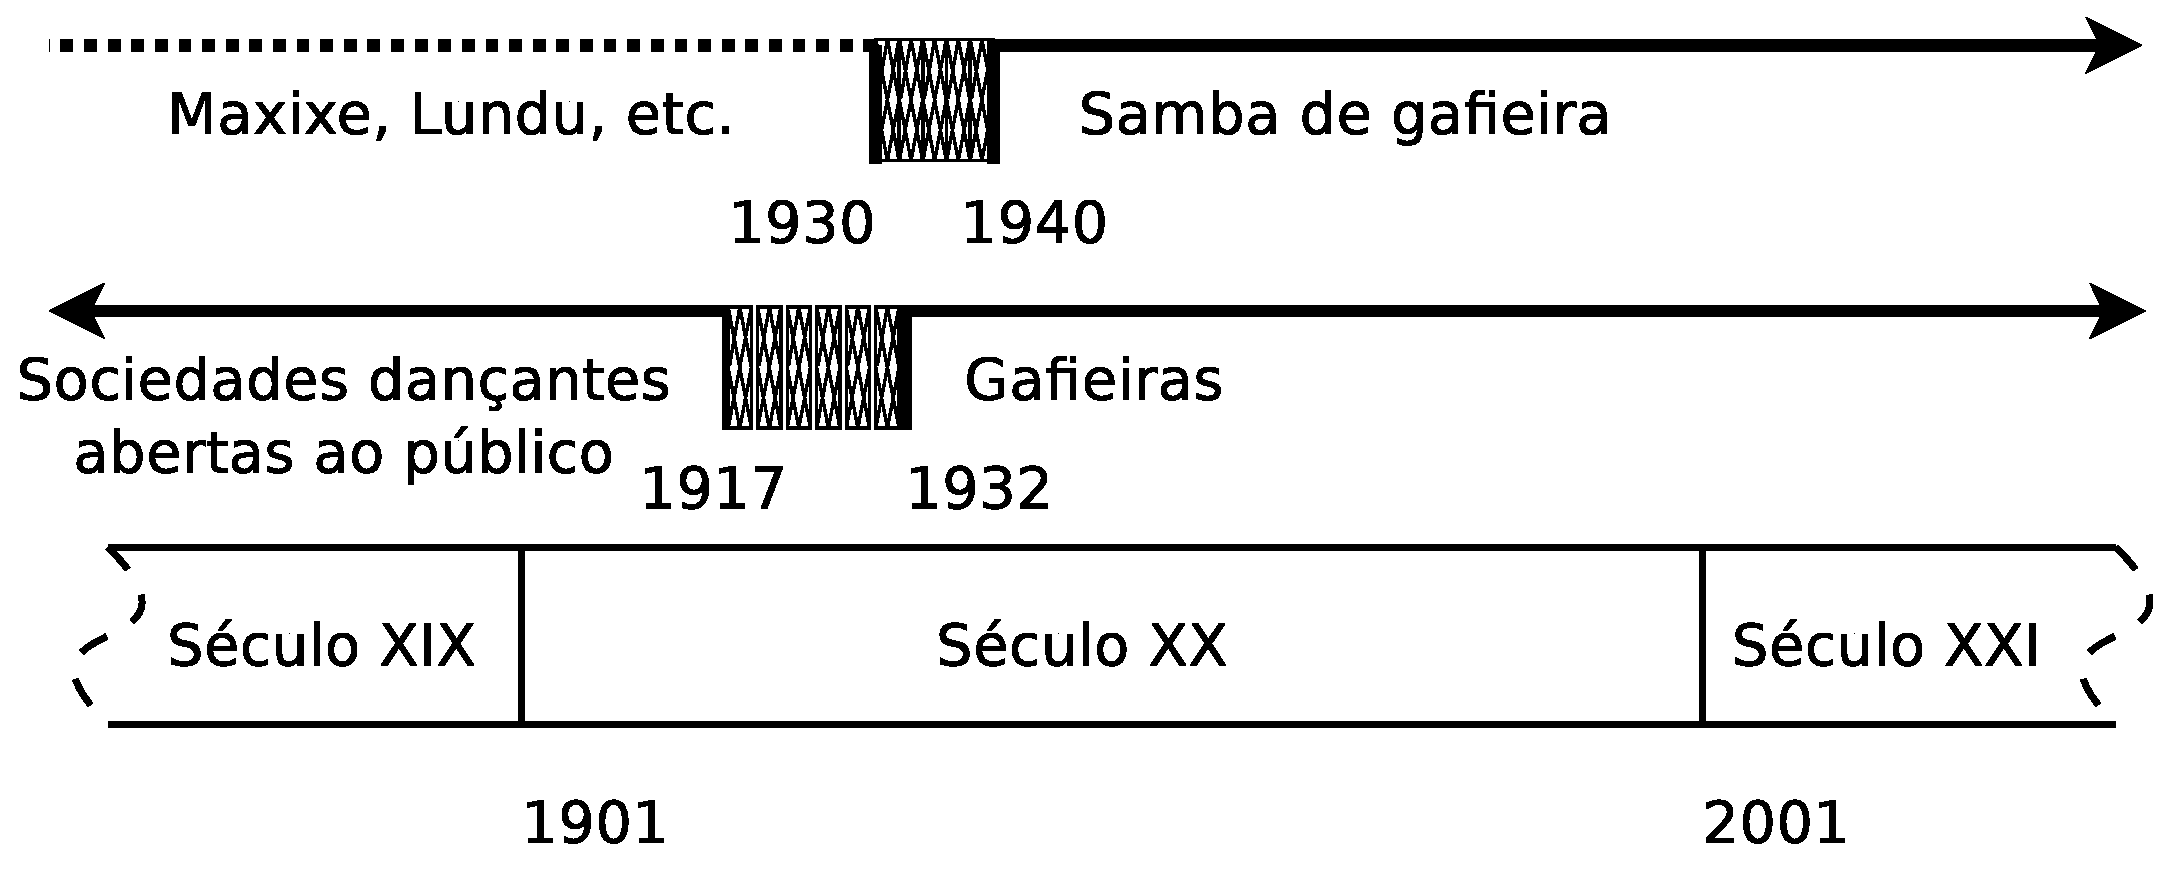
\includegraphics[width=1.0\textwidth]{chapters/cap-historia-sambagafieira/gafieira-crono.eps}
  \caption{ Cronologia da formação do samba de gafieira.}
\label{fig:sambagafieiracrono}
\end{figure}

%%%%%%%%%%%%%%%%%%%%%%%%%%%%%%%%%%%%%%%%%%%%%%%%%%%%%%%%%%%%%%%%%%%%%%%%%%%%%%%
%\clearpage
\section{Música para dançar samba de gafieira}
\label{subsec:gafieiradancaestilos}

Entre os estilos musicais em que o samba de gafieira (dança) se adapta bem, 
estão alguns dos subgêneros do samba; assim,
aqui mencionaremos algumas músicas que por sua graça, estilo e alegria,
a meu entender, podem ser dançados usando o samba de gafieira. Porem, 
estas músicas não pretendem ser máximos expoentes representativos do subgênero em que estão agrupados;
e sim uma indicação ou orientação ao leitor, 
para treinar sua dança usando músicas em que possa ser mais confortável a experiencia.

\begin{itemize}
\item \textbf{Samba de gafieira (música)}
\begin{example} ~
\begin{itemize}
%\item ``Samba de padua'' interpretado pelo grupo Turma da Gafieira.
\item ``Samba de morro'' interpretado pelo grupo Turma da Gafieira.
%\item ``Piston da gafieira'' de Billy Blanco, interpretado por Jorge Beiga.
\item ``Piston da gafieira'' de Billy Blanco, interpretado por Zeca pagodinho \cite{barbosa2014zeca}.
\item ``Beija-me'' de Roberto Martins e Mário Rossi, interpretado por Zeca pagodinho \cite{barbosa2014zeca}.
\item ``Pisei num despacho'' de Geraldo Pereira e Elpídio Viana, interpretado por Zeca pagodinho \cite{barbosa2014zeca}.
%\item ``Tive sim'' de Cartola, interpretado por Zeca pagodinho \cite{barbosa2014zeca}.
%\item ``Tarzan, o filho do alfaiate'' de Noel Rosa e Vadico, interpretado por Zeca pagodinho \cite{barbosa2014zeca}.
%\item ``Se você visse'' de Dino 7 cordas e Del Loro, interpretado por Zeca pagodinho \cite{barbosa2014zeca}.
\end{itemize}
\end{example} 

\item \textbf{Samba de breque}
\begin{example} ~
\begin{itemize}
\item ``Baile no elite'' interpretado por Casuarina.
\item ``Eu sou a marrom'' interpretado por Alicione.
%\item ``Hoje sou diferente'' interpretado por Lenita Rodrigues.
\item ``Pra levantar poeira'' interpretado por Bodhar.
\end{itemize}
\end{example} 

\item \textbf{Samba exaltação}
\begin{example} ~
\begin{itemize}
\item ``Aquarela do Brasil'' interpretado por Gal Costa.
\item ``Canta Brasil'' interpretado por Gal Costa.
\item ``Saudosa maloca'' interpretado pelo grupo Demônios da Garoa.
\end{itemize}
\end{example} 


\item \textbf{Pagode paulista (Sambalanço)}
\begin{example} ~
\begin{itemize}
\item ``Cheia de manias''  interpretado pelo grupo Raça Negra.
\end{itemize}
\end{example} 

\item \textbf{Partido alto}
\begin{example} ~
\begin{itemize}
%\item ``A língua'' interpretado por Beto lima.
\item ``Partido alto'' interpretado por Aleh.
\end{itemize}
\end{example} 

\item \textbf{Pagode}
\begin{example} ~
\begin{itemize}
\item ``Trilha do amor''  interpretado pelo Grupo Revelação. 
\item ``A batucada te pegou'' interpretado pelo Grupo Sou Muleke.
\item ``Dança da solidão'' interpretado por Pagode de Mesa do álbum Terra Brasil. 
\item ``Eu e você sempre'' interpretado por Jorge Aragão
\end{itemize}
\end{example} 

\item \textbf{Samba-canção (música)}
\begin{example} ~
\begin{itemize}
\item ``Só louco'' interpretado por Luiz Melodia.
\item ``Você é a fonte'' interpretado por  Quinteto em Branco e Preto.
\item ``Eu quero é sossego'' interpretado por Paulo Moura.
\end{itemize}
\end{example} 

\item \textbf{Bossa nova}
\begin{example} ~
\begin{itemize}
\item ``I don't know (Bossa mix)'' interpretado por Erika do álbum ``I don't know''
\item ``Human nature'' interpretado por Marcela Mangabeira.
\end{itemize}
\end{example} 


\item \textbf{Choro}
\begin{example} ~
\begin{itemize}
\item ``Choro de gafieira'' de Pixinguinha.
\item ``Chorinho de gafieira'' de Astor Silva.
\item ``Noites cariocas'' de Jacob do Bandolim.
\end{itemize}
\end{example} 


\item \textbf{Samba-choro}
\begin{example} ~
\begin{itemize}
\item ``Escurinho'' interpretado por Corina Magalhães.
\item ``Tico tico no fubá'' interpretado por Leci Brandão.
\end{itemize}
\end{example}

\end{itemize}

A Figura \ref{fig:gafieiradancaestilos} mostra um resumo de alguns dos 
subgêneros do samba onde pode ser dançado o samba de gafieira.
\begin{figure}[h]
  \centering
    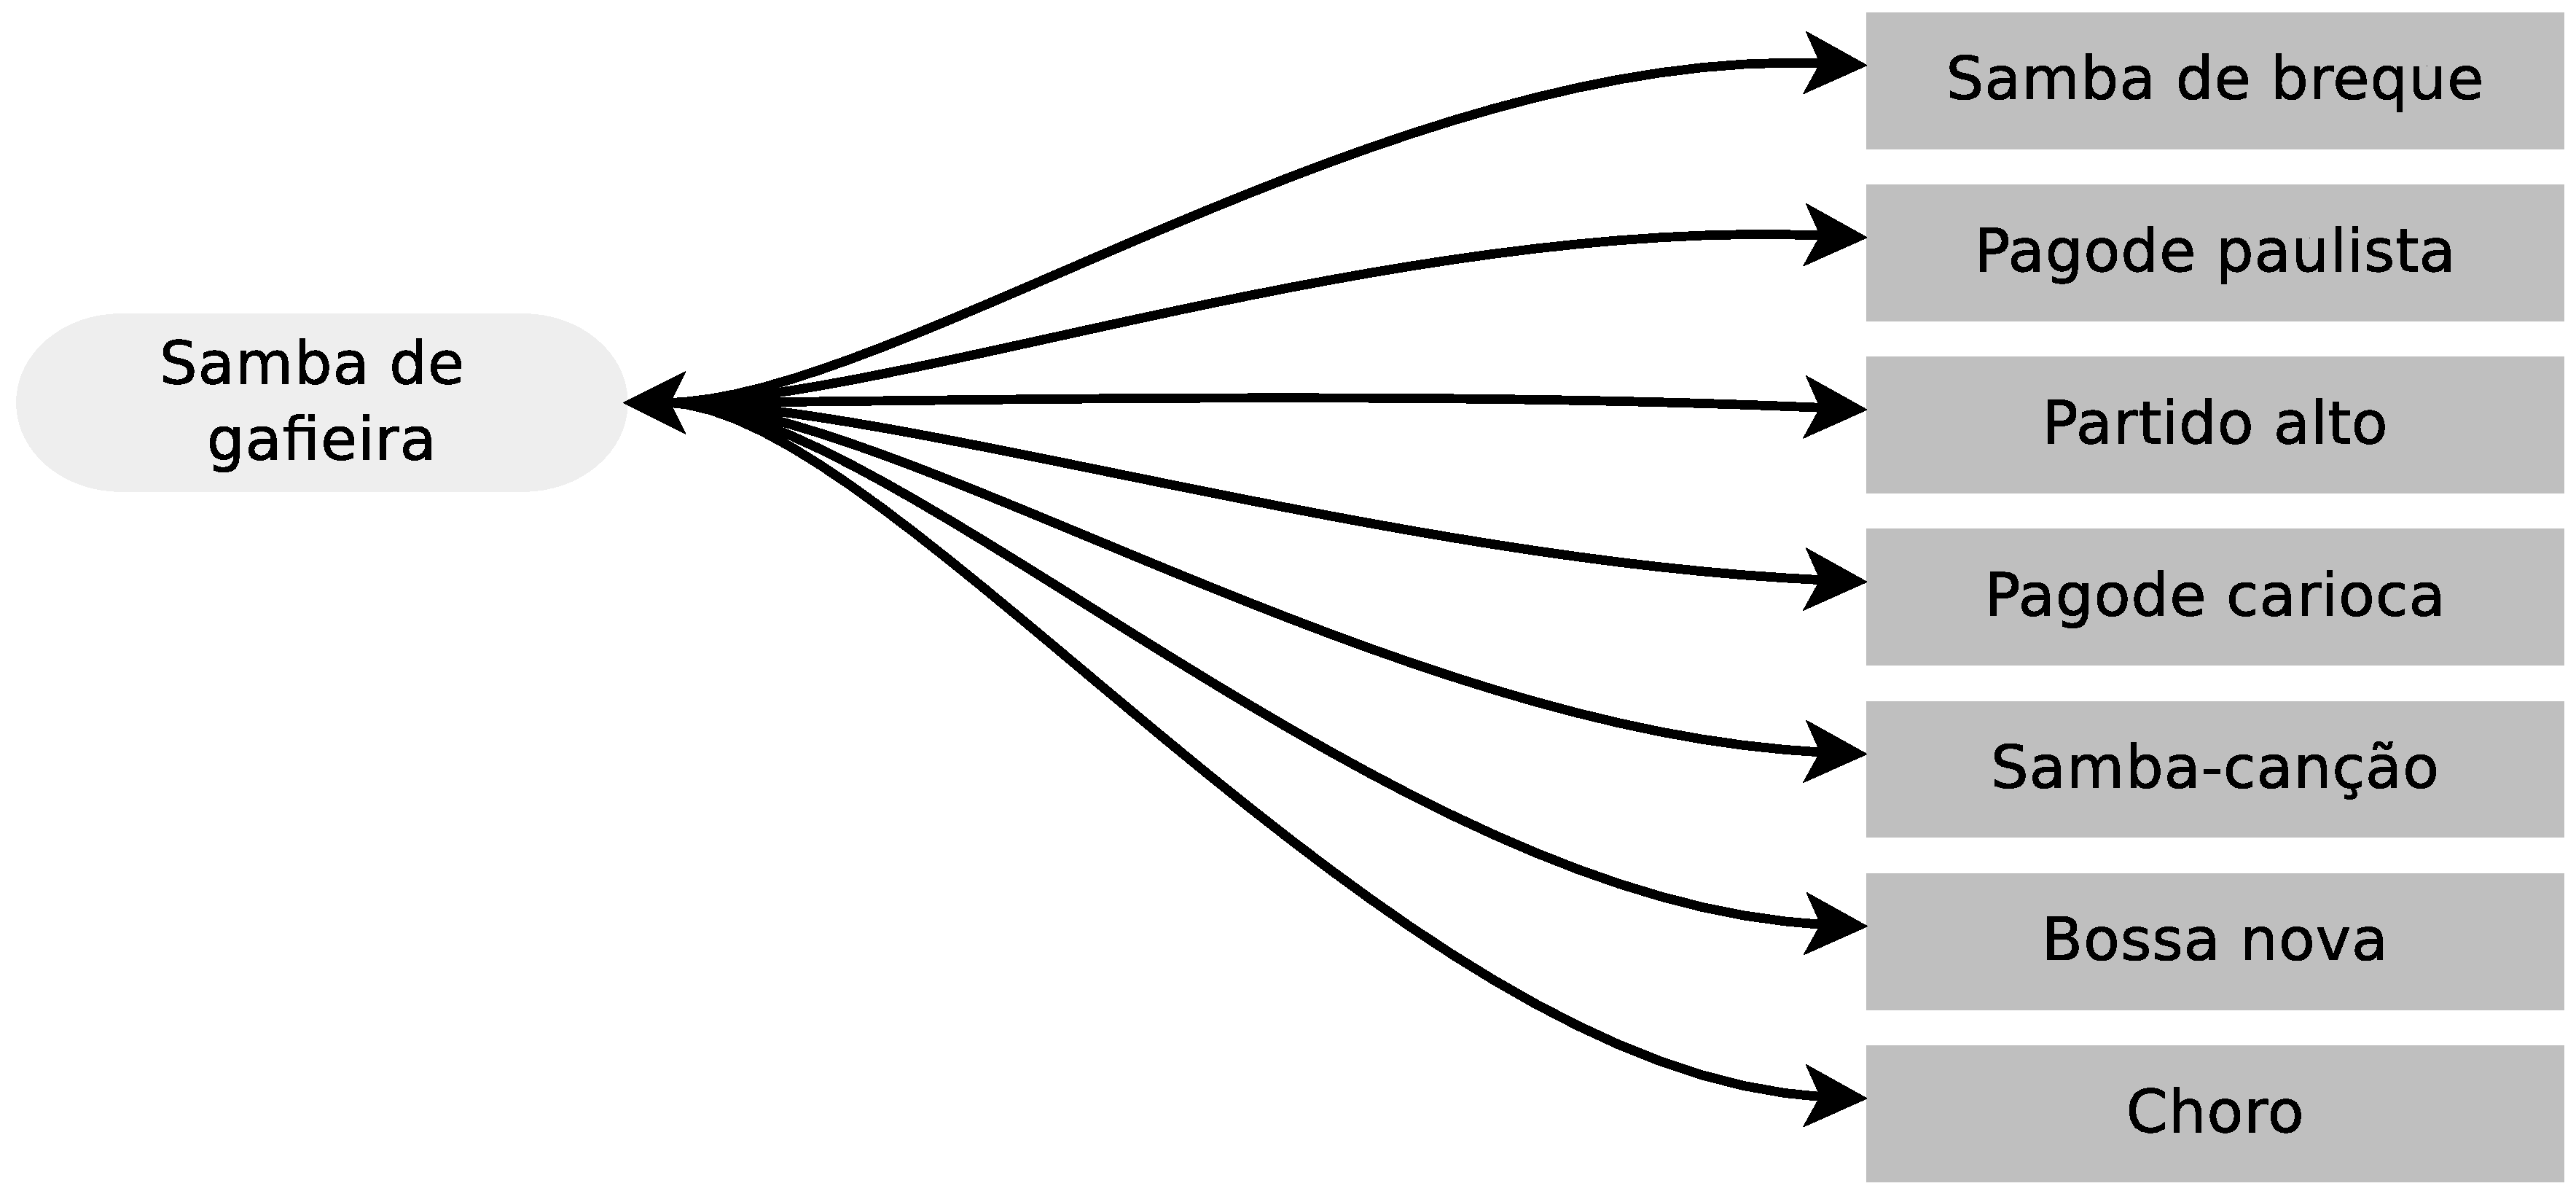
\includegraphics[width=0.9\textwidth]{chapters/cap-historia-sambagafieira/gafieiravcmusica.eps}
  \caption{ Subgêneros do samba onde pode-se dançar samba de gafieira.}
\label{fig:gafieiradancaestilos}
\end{figure}




\part{O samba e a dança de salão}
%%%%%%%%%%%%%%%%%%%%%%%%%%%%%%%%%%%%%%%%%%%%%%%%%%%%%%%%%%%%%%%%%%%%%%%%%%%%%%%%
%% Capitulo
%%%%%%%%%%%%%%%%%%%%%%%%%%%%%%%%%%%%%%%%%%%%%%%%%%%%%%%%%%%%%%%%%%%%%%%%%%%%%%%%
\chapterimage{chapter_head_2.pdf} % Chapter heading image

\chapter{Estilos de dança no samba}

%%%%%%%%%%%%%%%%%%%%%%%%%%%%%%%%%%%%%%%%%%%%%%%%%%%%%%%%%%%%%%%%%%%%%%%%%%%%%%%%
%%%%%%%%%%%%%%%%%%%%%%%%%%%%%%%%%%%%%%%%%%%%%%%%%%%%%%%%%%%%%%%%%%%%%%%%%%%%%%%%
\section{Que estilo de dança posso usar no samba (música)?}
\label{subsec:estilosdedanca}
A resposta mais simples poderia ser que, uma pessoa ao ser livre e independente,
pode escolher expressar-se na dança, de forma natural, como esta saia de si mesmo.
Porém, entrando em assuntos mais técnicos, 
e de acordo com os padrões socialmente mais comuns de ser achados atualmente;
existe um grupo de modalidades de dança, que por suas caraterísticas, 
são consideradas que se enquadram muito bem na música de alguns subgêneros do samba.

Assim, nas seguintes seções, serão descritos alguns dos estilos de dança para a música do samba,  
que podemos achar nos salões e locais de dança no Brasil;
estes serão agrupados em estilos \textbf{dançados em pares}, e os que são \textbf{dançados de forma separada}. 


%%%%%%%%%%%%%%%%%%%%%%%%%%%%%%%%%%%%%%%%%%%%%%%%%%%%%%%%%%%%%%%%%%%%%%%%%%%%%%%%
\section{Estilos dançados em pares}
\label{subsec:estilosdedancapares}
Entre os estilos que se dançam a dois, existentes na atualidade, temos \cite[pp. 134]{perna2002samba}:

%%%%%%%%%%%%%%%%%%%%%%%%%%%%%%%%%%%%%%%%%%%%%%%%%%%%%%%%%%%%%%%%%%%%%%%%%%%%%%%%
\subsection{Samba de gafieira (dança)} 
\index{Dança!Samba de gafieira}
É uma dança a dois que pode ser executada na maioria dos subgêneros do samba (música),
tendo exceções em: samba-enredo, samba reggae (música), samba rock (música), 
marcha, marcha-rancho e maxixe (música);
nos seus origens este tipo de dança era chamado de samba-batucada  \cite[pp. 134]{perna2002samba}, 
mais detalhes do samba de gafieira no Capítulo \ref{cap:sambagafieira}.

%%%%%%%%%%%%%%%%%%%%%%%%%%%%%%%%%%%%%%%%%%%%%%%%%%%%%%%%%%%%%%%%%%%%%%%%%%%%%%%%
\subsection{Samba liso} 
\label{subsec:sambalisodef}
\index{Dança!Samba liso}
%\index{Dança!Samba caminhado}
Atualmente se dança similarmente ao samba de gafieira, 
porém com um estilo mais elegante, sem ginga né passos de efeito, e dizer é uma dança mais ``lisa'';
se dança bem em: samba-canção, bossa nova e choro \cite[pp. 134]{perna2002samba}.

\PRLsep{Referencias ao samba liso (1917-1933):} 

Podemos achar uma referencia interessante ao uso do termo \textbf{samba} e \textbf{liso}  no livro 
``Feitiço decente: Transformações do samba no Rio de Janeiro (1917-1933)'' (2001),
onde se pode intuir a procedência deste nome ou denominação, 
quando se faz referencia a um comentário de João da Baiana sobre o samba-de-umbigada e o samba de roda \cite[pp. 109]{sandroni2001feitico}: 
\begin{citando}
Nós tirávamos um verso e o pessoal sambava, um de cada vez ... 
Um saía para tirar o outro.
Se fosse a ``liso'' era só umbigada, mas se fosse para pegar ``duro'' já era capoiragem. 
\end{citando}
Pelo que no livro se comenta, que para o dançarino solista  escolher a seu sucessor podiam
existir duas modalidades, dependendo do tipo de roda, em ``samba liso'' (com umbigada) ou em ``samba duro'' 
(ou batucada\footnote{No qual a umbigada é substituída por uma pernada \cite[pp. 109]{sandroni2001feitico},
para mais detalhes ir a página \pageref{ref:batuquedanca}.}) \cite[pp. 109]{sandroni2001feitico}.
Esta referencia 
é particularmente interessante, pois como veremos na Seção \ref{cap:sambagafieira},
nos primórdios do samba nas gafieiras, existiam 3 modalidades em que esta era dançada: samba-canção (dança),
\textbf{samba-batucada} (dança)\footnote{Que 
é o nome com que era conhecido originalmente a atual samba de gafieira \cite[pp. 143]{perna2002samba}.} 
e \textbf{samba-liso} \cite[pp. 143]{perna2002samba};
estas duas últimas, não são as mesmas danças dos samba-de-umbigada, 
e sim novas formas de dançar o samba num ambiente mais civilizado como o salão de dança;
porém, estes nomes conservavam a mesma nomenclatura, na descrição 
da relativa relação à tosquedade dos movimentos, entre uma dança mais suave ou lisa, 
e outra dura ou batucada.

%%%%%%%%%%%%%%%%%%%%%%%%%%%%%%%
\PRLsep{Referencias ao samba liso (1950-1953)}


Na ``Hemeroteca Digital Brasileira'' da Fundação Biblioteca Nacional,
não tem-se achado referencias\footnote{ Foram achadas,
2, 5, 3, 1 e 1 referencias brutas para as décadas de 1930, 1940, 1960, 1970 e 1980 respetivamente;
porém, estas não eram relativas ao samba liso de salão ou eram falsos acertos.} 
à frase ``\textbf{samba liso}'', nas décadas de 1930, 1940, 1960, 1970 e 1980;
as referencias achadas correspondem à década de 1950\footnote{Especificamente entre os anos 1950 e 1953.}  
com uma total de 327 referencias;
de todas estas, 326 correspondem à forte campanha 
de marketing do livro
``Como aprender a dançar'', 
de Gino Forniciari. 
Por exemplo, podemos achar a primeira referencia em ``O Jornal'' (RJ),
do dia 17 de setembro de 1950, onde se pode ler \cite[3ra seção pp. 9]{jornalanunciodanca1}:
\begin{citando}
\begin{center}
Como aprender a dançar\\
4a edição ampliada
\end{center}
Com a nova dança, ``Baião'', \textbf{Samba liso}, e os
últimos passos de Bolero, Rumba, Swing, contendo
120 gráficos 330 passos, facilitando as senhoritas 
e cavalheiros a aprenderem em suas próprias 
casas em 10 dias apenas, no princípio sem
companheiro ou companheira. Método de ritmos modernos
pelo Prof. Gino Fornaciari, 
Diretor e Prof. do ``CURSO PRATICO DE DANÇAS RITZ''.
Aulas particulares, rua da Liberdade, 120.
Preço: Cr\$ 45,00 -- Pedidos pelo reembolso posta 
-- com o autor -- Caixa Postal, 649 -- SÃO PAULO 
\end{citando}
Todos estes anúncios vem na maioria das vesses acompanhados com um desenho como
o mostrado na Figura \ref{fig:desenholivrodanca1}, que indica todos os estilos de dança abordados no livro;
e se diferencia entre dançar \textbf{samba} e \textbf{samba liso}.
\begin{figure}[h]
  \centering
    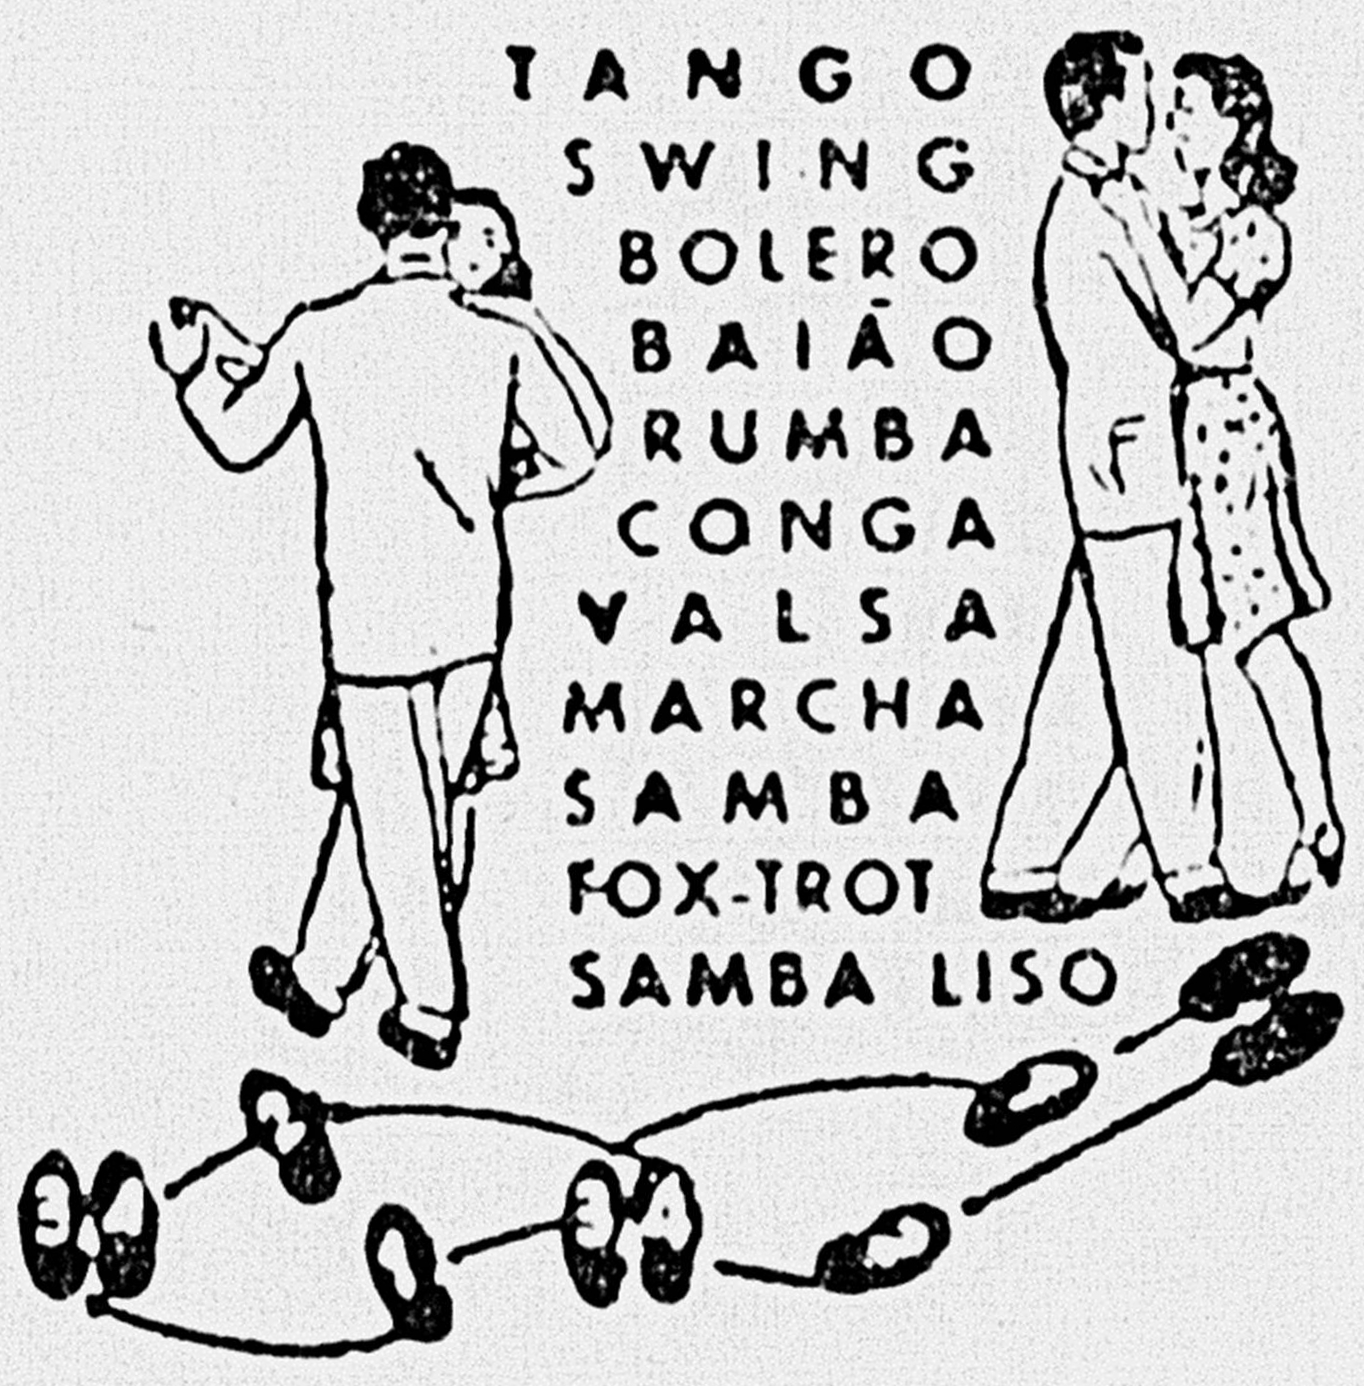
\includegraphics[width=0.6\textwidth]{chapters/cap-historia-dancasamba/comoaprenderdancar.jpg}
  \caption{Desenho da publicidade do livro ``Como aprender a dançar'' de Gino Forniciari,
publicado, no dia 17 de fevereiro de 1952, em ``Sport Ilustrado'' \cite[pp. 22]{sportlivropublidanca}.}
\label{fig:desenholivrodanca1}
\end{figure}
Ja no decorrer do livro o autor, define o samba de salão e apresenta 3 modalidades,
de ser dançado, sendo uma destas o samba liso \cite[pp. 61]{fornaciari1950aprender}.
É interessante ressaltar que a segunda edição deste livro, lançada no ano de 1947,
não tinha nenhuma referencia ao samba liso, ficando a incógnita se esta omissão era
porque a modalidade era pouco conhecida ou recente nessa época, ou por desconhecimento do autor.



%%%%%%%%%%%%%%%%%%%%%%%%%%%%%%%
A outra referencia achada na ``Hemeroteca Digital Brasileira'' da Fundação Biblioteca Nacional,
com a frase ``samba liso'', na década de 1950, foi a publicada o dia 26 de agosto de 1951,
no ``Diário do Nordeste'' de Caixas do Sul (RS), numa cronica de Walter Brugger da sua viagem por Europa,
num articulo titulado ``Genova! Primeiro Contato com a Europa!'',
onde se pode ler \cite[pp. 10]{nordestesambalisocronica}:
\begin{citando}
Ao nosso lado, numa área 
descoberta uma orquestra tocava para
quem quizesse dançar.
Repentinamente ouvimos uma melodia muito
nossa conhecida. Era o imortal ``Tico-Tico no Fubá''... Todavia,
apesar da melodia correta, o ritmo
era bastante falho. Continuando 
com os ritmos brasileiros, a orquestra 
tocou ainda ``Chiquita Bacana'',
mas em tempo de samba e ``Aquarela do Brasil''.
O que porém nos 
deixou mais atônitos foi o modo como 
era dançado o nosso samba. De 
brasileiro não tinha nada. Pelo que 
vimos, o \textbf{samba ``liso''} lhes é desconhecido 
e cada um procura ``requebrar'' o corpo mais que o outro,
mas de uma forma como nós só 
conhecemos no cinema mexicano. 
O meu amigo dava gostosas risadas e não era para menos,
ante a comicidade do espetáculo, tão 
impossível no Brasil quanto desconhecido para nós.
\end{citando}


%%%%%%%%%%%%%%%%%%%%%%%%%%%%%%%
\PRLsep{Referencias ao samba liso (1955)}

Outra referencia ao \textbf{samba liso}, pode ser achada no livro ``Manual de Danças Gaúchas'' (1955)
onde se afirma que \cite[pp. 77]{cortesmanual}: 
\begin{citando}
A polquinha, como dança especifica, é executada por pares enlaçados,
mediante passos-de-marcha (É correograficamente  semelhante ao chamado 
\textbf{samba liso} ou \textbf{samba caminhado} dos salões urbanos).
\end{citando}~\\

%%%%%%%%%%%%%%%%%%%%%%%%%%%%%%%
\PRLsep{Descrição do samba liso (1959)}

Era uma dança na qual se bamboleia o corpo e se dançava sem flexionar os joelhos \cite[pp. 58]{freitas1959danca} \cite[pp. 143]{perna2002samba},
era dançado usando 4 movimentos (em 2 compassos) \cite[pp. 62]{freitas1959danca} \cite[pp. 143]{perna2002samba}.
Sobre os passos usados nessa época, 
na Figura \ref{fig:samba-liso-basico-frente} se mostra o passo básico para a frente do samba liso,
e na  Figura \ref{fig:samba-liso-basico-frente} o mesmo movimento para trás; 
em ambos casos se usa os 4 movimentos antes mencionados, e a cor cinza indica a posição inicial \cite[pp. 63]{freitas1959danca}. 
\begin{figure}[h]
    \centering
    \begin{subfigure}[b]{0.4\textwidth}
        \centering
        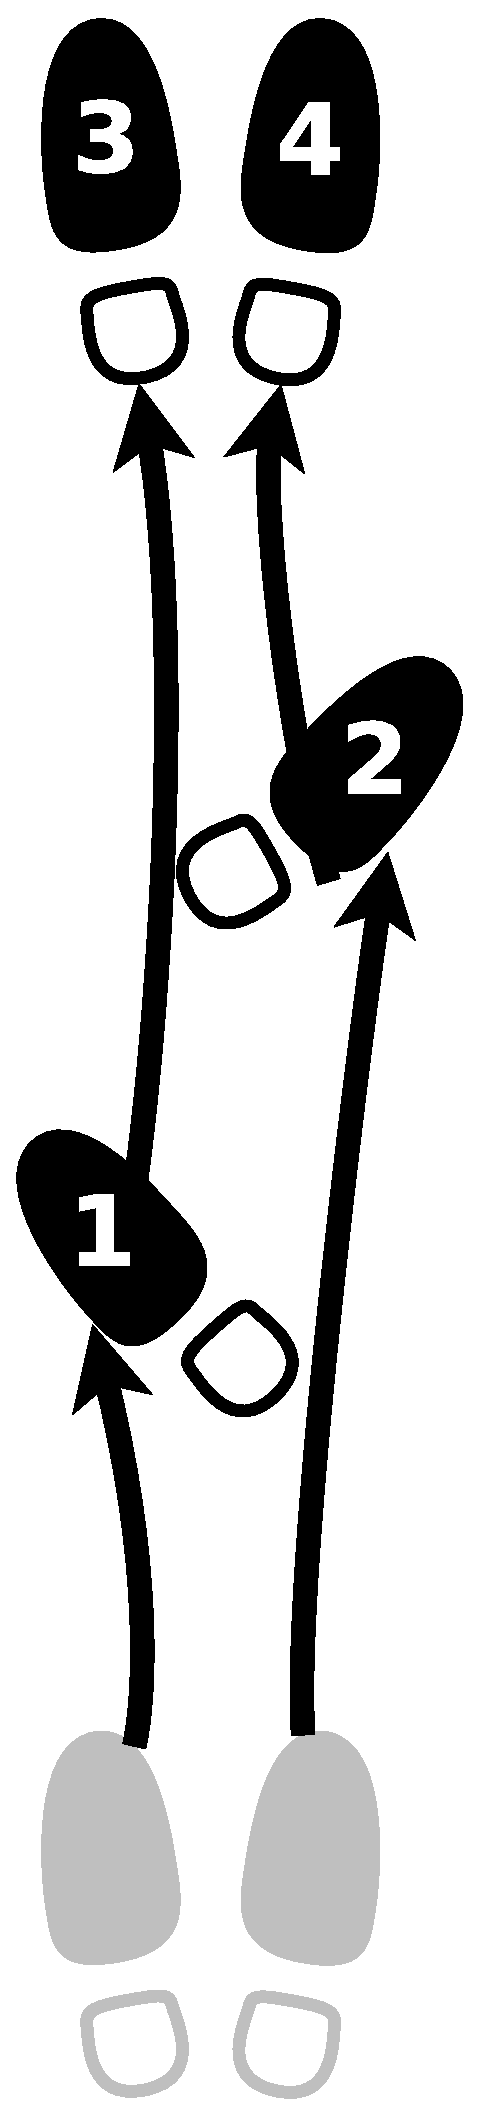
\includegraphics[width=0.25\textwidth]{chapters/cap-historia-dancasamba/samba-liso-basico-frente.eps}
        \caption{Passo básico para a frente.}
        \label{fig:samba-liso-basico-frente}
    \end{subfigure}
    ~ %add desired spacing between images, e. g. ~, \quad, \qquad, \hfill etc. 
      %(or a blank line to force the subfigure onto a new line)
    \begin{subfigure}[b]{0.4\textwidth}
        \centering
	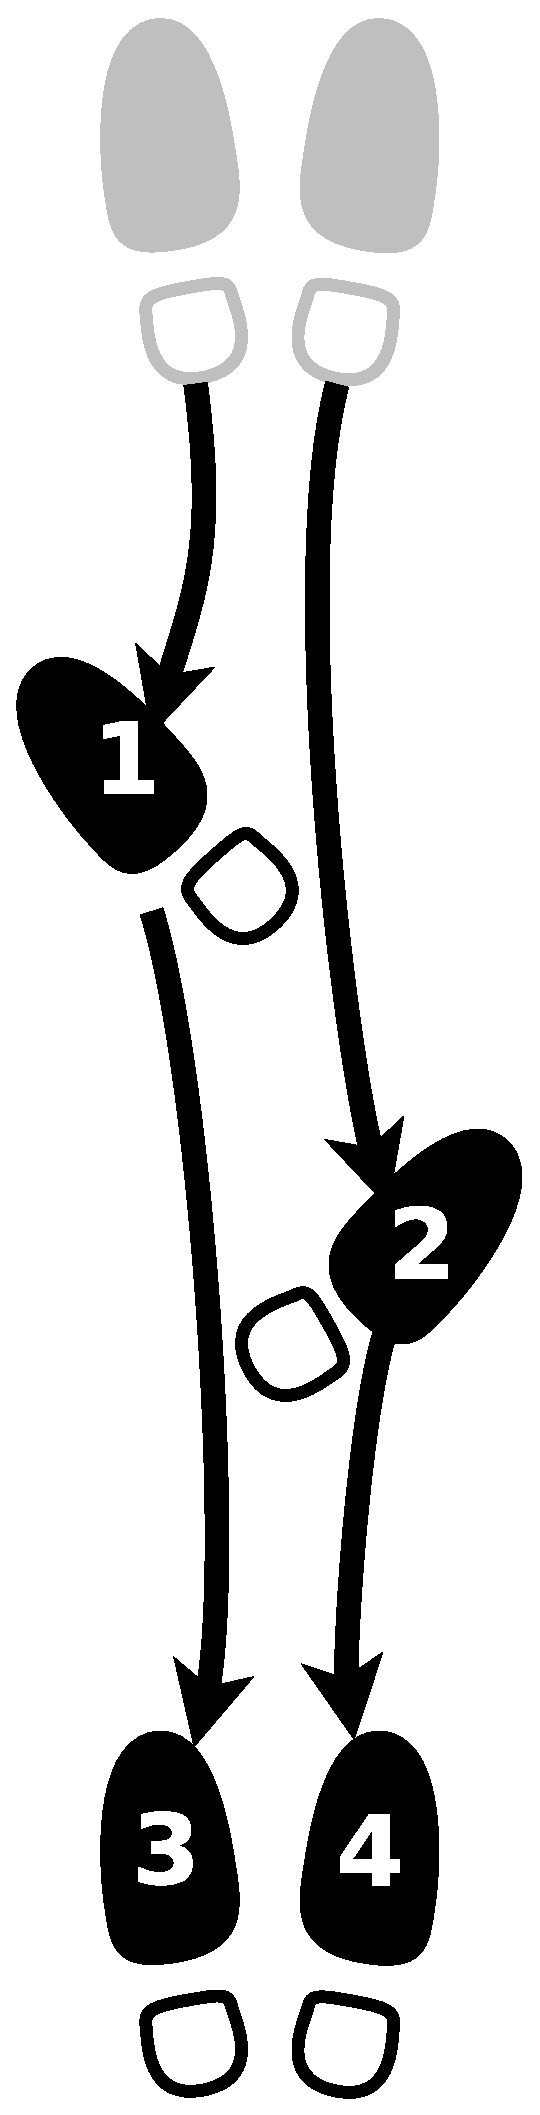
\includegraphics[width=0.25\textwidth]{chapters/cap-historia-dancasamba/samba-liso-basico-tras.eps}
        \caption{Passo básico para trás.}
        \label{fig:samba-liso-basico-tras}
    \end{subfigure}
    \caption{Samba liso da década de 1950.}\label{fig:samba-liso-basico}
\end{figure}

%%%%%%%%%%%%%%%%%%%%%%%%%%%%%%%%%%%%%%%%%%%%%%%%%%%%%%%%%%%%%%%%%%%%%%%%%%%%%%%%
\subsection{Samba pagode} 
\index{Dança!Samba pagode}
É um estilo de dança a dois, originário de São Paulo, 
é uma dança com poucos deslocamentos \cite[pp. 134]{perna2002samba}.
É um estilo de dança adaptado para ser dançado com o pagode paulista,
também chamado como Sambalanço\footnote{Ver página \pageref{ref:sambalanco}.}.
%% https://www.youtube.com/watch?v=SfvoiXOGPn4
Ao igual que o sambalanço teve duas épocas com estilos musicais diferentes,
a dança \textbf{samba pagode}, sofreu também transformações acompanhando essas tendencias.
Podem-se observar atualmente 3 tipos de passo base: 
%% https://www.youtube.com/watch?v=rq1uhNXySds 
%% https://www.youtube.com/watch?v=SfvoiXOGPn4

O miudinho, que é um passo que se realiza abraçado com o par e de forma espelhada com este,
onde se executam 3 twist\footnote{É importante ter um sapato que deslise bem.} no lugar, 
só trocando de peso entre os pés, seguindo um ritmo, rápido-rápido-lento;
este movimento se executa simetricamente duas vesses para formar um ciclo completo,  
uma vez iniciando com o peso do corpo para o pé direito\footnote{Quando o primeiro twist é horário.} e a outra com o esquerdo.

O passo básico lateral, se realiza abraçado com o par  e de forma espelhada com este, 
é similar ao passo básico de capoeira,
ou a base aberta do forró\footnote{Só que aqui é abraçados.},
onde se produzem 3 movimento seguindo um ritmo, rápido-rápido-lento,
no primeiro momento, um pé vai para atrás, 
no segundo o outro ajeita sua posição deslocando-se levemente, 
procurando o centro e o equilíbrio do par dançante, e
no terceiro o pé que estava atrás volta ao lado do outro,
este movimento se executa simetricamente duas vesses para formar um ciclo completo,  
uma vez iniciando com pé direito e a outra com o esquerdo.
Este movimento é interessante para fazer deslocamento, 
que são realizados principalmente nesse primeiro movimento com o pé atrás, 
só que agora apontando para uma direção especifica.

A caidinha, se realiza abraçado com o par, 
este passo é similar ao picadilho (picadinho) de samba de gafieira,
porém com um deslocamento similar ao repique do forró;
no pagode paulista este movimento se executa seguindo um ritmo, rápido-rápido-lento,
onde o seguidor faz um movimento similar ao miudinho antes mencionado,
enquanto que o condutor tem uma liberdade criativa no 
seu movimento\footnote{O mesmo que acontece no picadilho de samba de gafieira.} 
enquanto respeite o ritmo, rápido-rápido-lento.

%%%%%%%%%%%%%%%%%%%%%%%%%%%%%%%%%%%%%%%%%%%%%%%%%%%%%%%%%%%%%%%%%%%%%%%%%%%%%%%%
\subsection{Samba rock (dança)}
\index{Dança!Samba rock}
É um estilo de dança a dois, realizado nos bailes ``black'' paulistas desde a década de 1960, 
sendo esta uma dança variante das danças do swing/rock e parente do soltinho carioca \cite[pp. 135]{perna2002samba}.
se dança bem em: Swing, samba rock (música), samba com suingue e samba-funk \cite[pp. 135,138]{perna2002samba}.
O samba rock se dança de mão dadas, e se carateriza por ter muitas voltas,
executadas na maior parte de vesses pelas  seguidores;
porém, é uma dança estacionaria pois os dançantes rara vez se deslocam pelo salão, 
e pelo contrario ficam trabalhando seus passos num mesmo lugar  \cite[pp. 135,138]{perna2002samba}.
Quando um espectador externo vê esta dança perceberá muitas figuras usando só os braços,
com enrosques, voltas, enlaces, etc.
Enquanto os pés de ambos dançarinos fazem uma mesma marcação, num constante e repetitivo rápido-rápido-lento,
caminhando unicamente sobre um circulo imaginário no chão, uma vez em sentido horário e outra em anti-horário.

%%%%%%%%%%%%%%%%%%%%%%%%%%%%%%%%%%%%%%%%%%%%%%%%%%%%%%%%%%%%%%%%%%%%%%%%%%%%%%%%
\subsection{Samba funkeado}
\label{subsec:sambafunkeado}
\index{Dança!Samba funkeado}
Também é chamado de estilo Jimmy de Oliveira ou simplesmente  samba Jimmy, 
em aluição a seu criador.
Este estilo de dança a dois foi criado no ano de 1998.
Com muito esforço Jimmy, num período aproximado de 6 meses, 
criou a estrutura da dança, desde iniciante ate avançado;
no ano de 1999 ele  chamou a esse estilo como ``samba quebrado'';  
posteriormente renomeou  para ``samba Jimmy'', 
recebeu algumas criticas e no ano 2001 decidiu renomeá-lo para ``samba funk'',
porém isto trouxe confusões   ao ser associado com a música funk, existente em Rio de Janeiro,
muito distante da proposta dele, e
finalmente a meados do 2005 ele decidiu chamá-lo ``samba funkeado''  \cite{sambafunkeadoJimmyDeOliveiraPart1}.
A Figura \ref{fig:funkeadocrono1} mostra a cronologia de nomes para este estilo.
\begin{figure}[h]
  \centering
    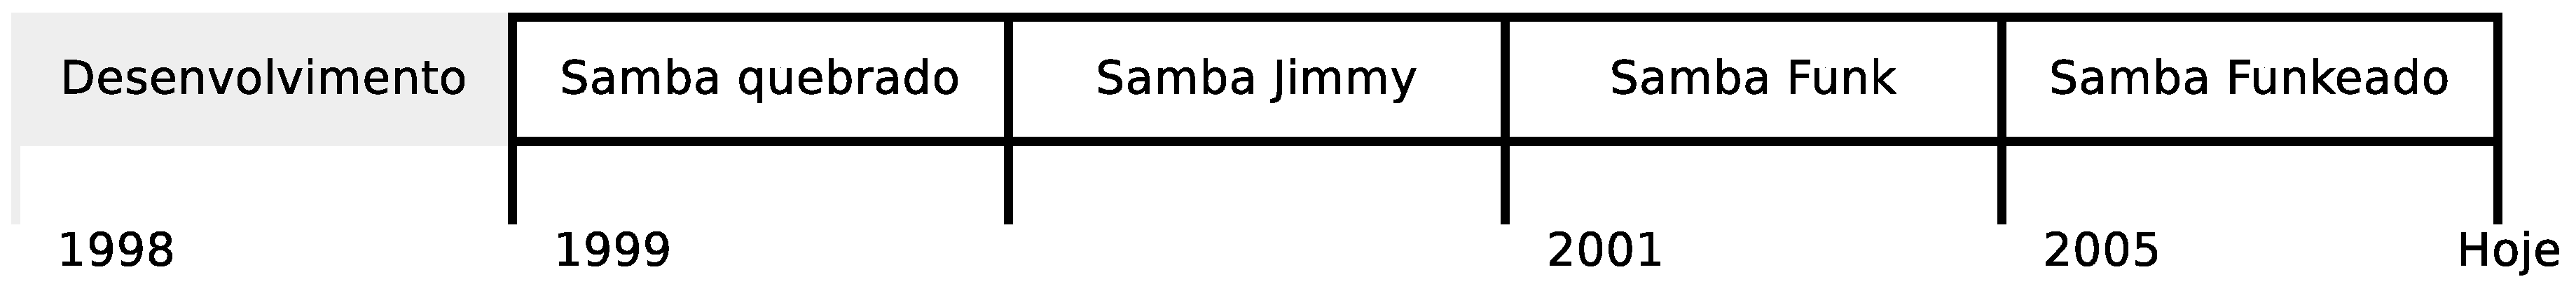
\includegraphics[width=1.0\textwidth]{chapters/cap-historia-dancasamba/sambafunkeado.eps}
  \caption{Cronologia dos nomes para samba funkeado.}
\label{fig:funkeadocrono1}
\end{figure}

O estilo foi criado para, em palavras de Jimmy: ``contribuir em função da música'', 
numa tentativa de agregar movimento em coerência como as músicas que ele gostava;
sendo estas interpretadas por:
Djavan, Jorge Ben Jor, Tim Maia, Leny Andrade \cite{sambafunkeadoJimmyDeOliveiraPart1}, que em seu momento, 
presentaram músicas de bossa nova ou que eram influenciadas pelo jazz, 
funk norte-americano ou ``black music'' \cite{sambafunkeadoJimmyDeOliveiraPart1} \cite{sambafunkeadoJimmyDeOliveiraPart3},
Jimmy indica que seu estilo procura ir em função da música escutada no brasil, 
e que a maioria da música atual é influenciada pelo funk norte-americano;
como a música de: João Sabiá. 

 
Seguindo a professora de dança Erika Ikuno, no 2003 
mediante o lançamento do album ``A procura da batida perfeita'' do rapper Marcelo D2
se presentó um trabalho musical brasileiro realativo ao samba que aos olhos de Jimmy e ela
envolvia todo o que procuravam musicalmente quando dançavam samba funkeado,
de modo que a partir de entonces a maioria dos dançarinos inciarom a preferir gêneros 
musicais brasileiros (samba com hiphop) para dançar samba funkeado \cite[pp. 92]{filho2016tango},
pois ate então a tedencia era escolher gêneros musicais estrangeiros.

O samba funkeado pode ser dançado em gêneros como ``black music'',
em pagodes funkeados (Sorriso maroto, Netinho de Paula, pixote, etc.), 
em sambas com influencia do jazz \cite{sambafunkeadoJimmyDeOliveiraPart3}, etc.

O samba funkeado tem 3 tendencias ou estruturas  \cite{sambafunkeadoJimmyDeOliveiraPart2}:
\begin{itemize}
\item \textbf{Samba funkeado}, primigênio.
\item \textbf{Samba funkeado fragmentado}; exemplo: um movimento que é de sentar, que gastaria um tempo, 
passa a ter ate 3 tempos; é dizer, fragmenta os movimentos. 
O fragmentado também permite dançar com movimentações em contrapeso no par de dança.
\item \textbf{Samba funkeado samsurf}, com uma postura mais curvada.
\end{itemize}

%e em seu ídolo Michael Jackson \cite{sambafunkeadoJimmyDeOliveira2}.
 
%%%%%%%%%%%%%%%%%%%%%%%%%%%%%%%%%%%%%%%%%%%%%%%%%%%%%%%%%%%%%%%%%%%%%%%%%%%%%%%%
\subsection{Samba internacional}
\label{subsec:DancaSambaInternacional} 
\index{Dança!Samba internacional}
É um estilo de dança a dois, influenciado pelo maxixe;
se dança principalmente fora do Brasil e existem basicamente dois estilos: 
o estilo internacional e o estilo norte-americano (EE.UU.) \cite[pp. 134-135]{perna2002samba}.

O samba introduzida a EE.UU. é uma dança de salão muito animada, 
com música de ritmo alegre, que sugere um estilo de movimento que pode
chegar a ser tão turbulento quanto os movimentos do Jive.
O padrão de passos básicos é similar aos achados no Fox-Trot e o Waltz;
%sendo estes: fwd-swd-close ... bwd-swd-close; e
com uma distribuição de tempos que segue uma sequência: 
quick-quick-slow\footnote{Rápido-rápido-lento.} ... quick-quick-slow \cite{parson2016ballroom}.

Observando os campeonatos internacionais nos quais este estilo é usado, 
se percebe que o samba internacional é dançado em qualquer estilo musical que
tenha sotaque ou de a impressão de ter raiz afro-latina.

%%%%%%%%%%%%%%%%%%%%%%%%%%%%%%%%%%%%%%%%%%%%%%%%%%%%%%%%%%%%%%%%%%%%%%%%%%%%%%%%
\subsection{Relações entre os subgêneros do samba e os estilos dançados em pares}

A Figura \ref{fig:sambadavavsmusica} mostra as relações entre os estilos de dança a dois (na esquerda),
 e alguns subgêneros do samba (na direita) \cite[pp. 134-138]{perna2002samba}.

\begin{figure}[h]
  \centering
    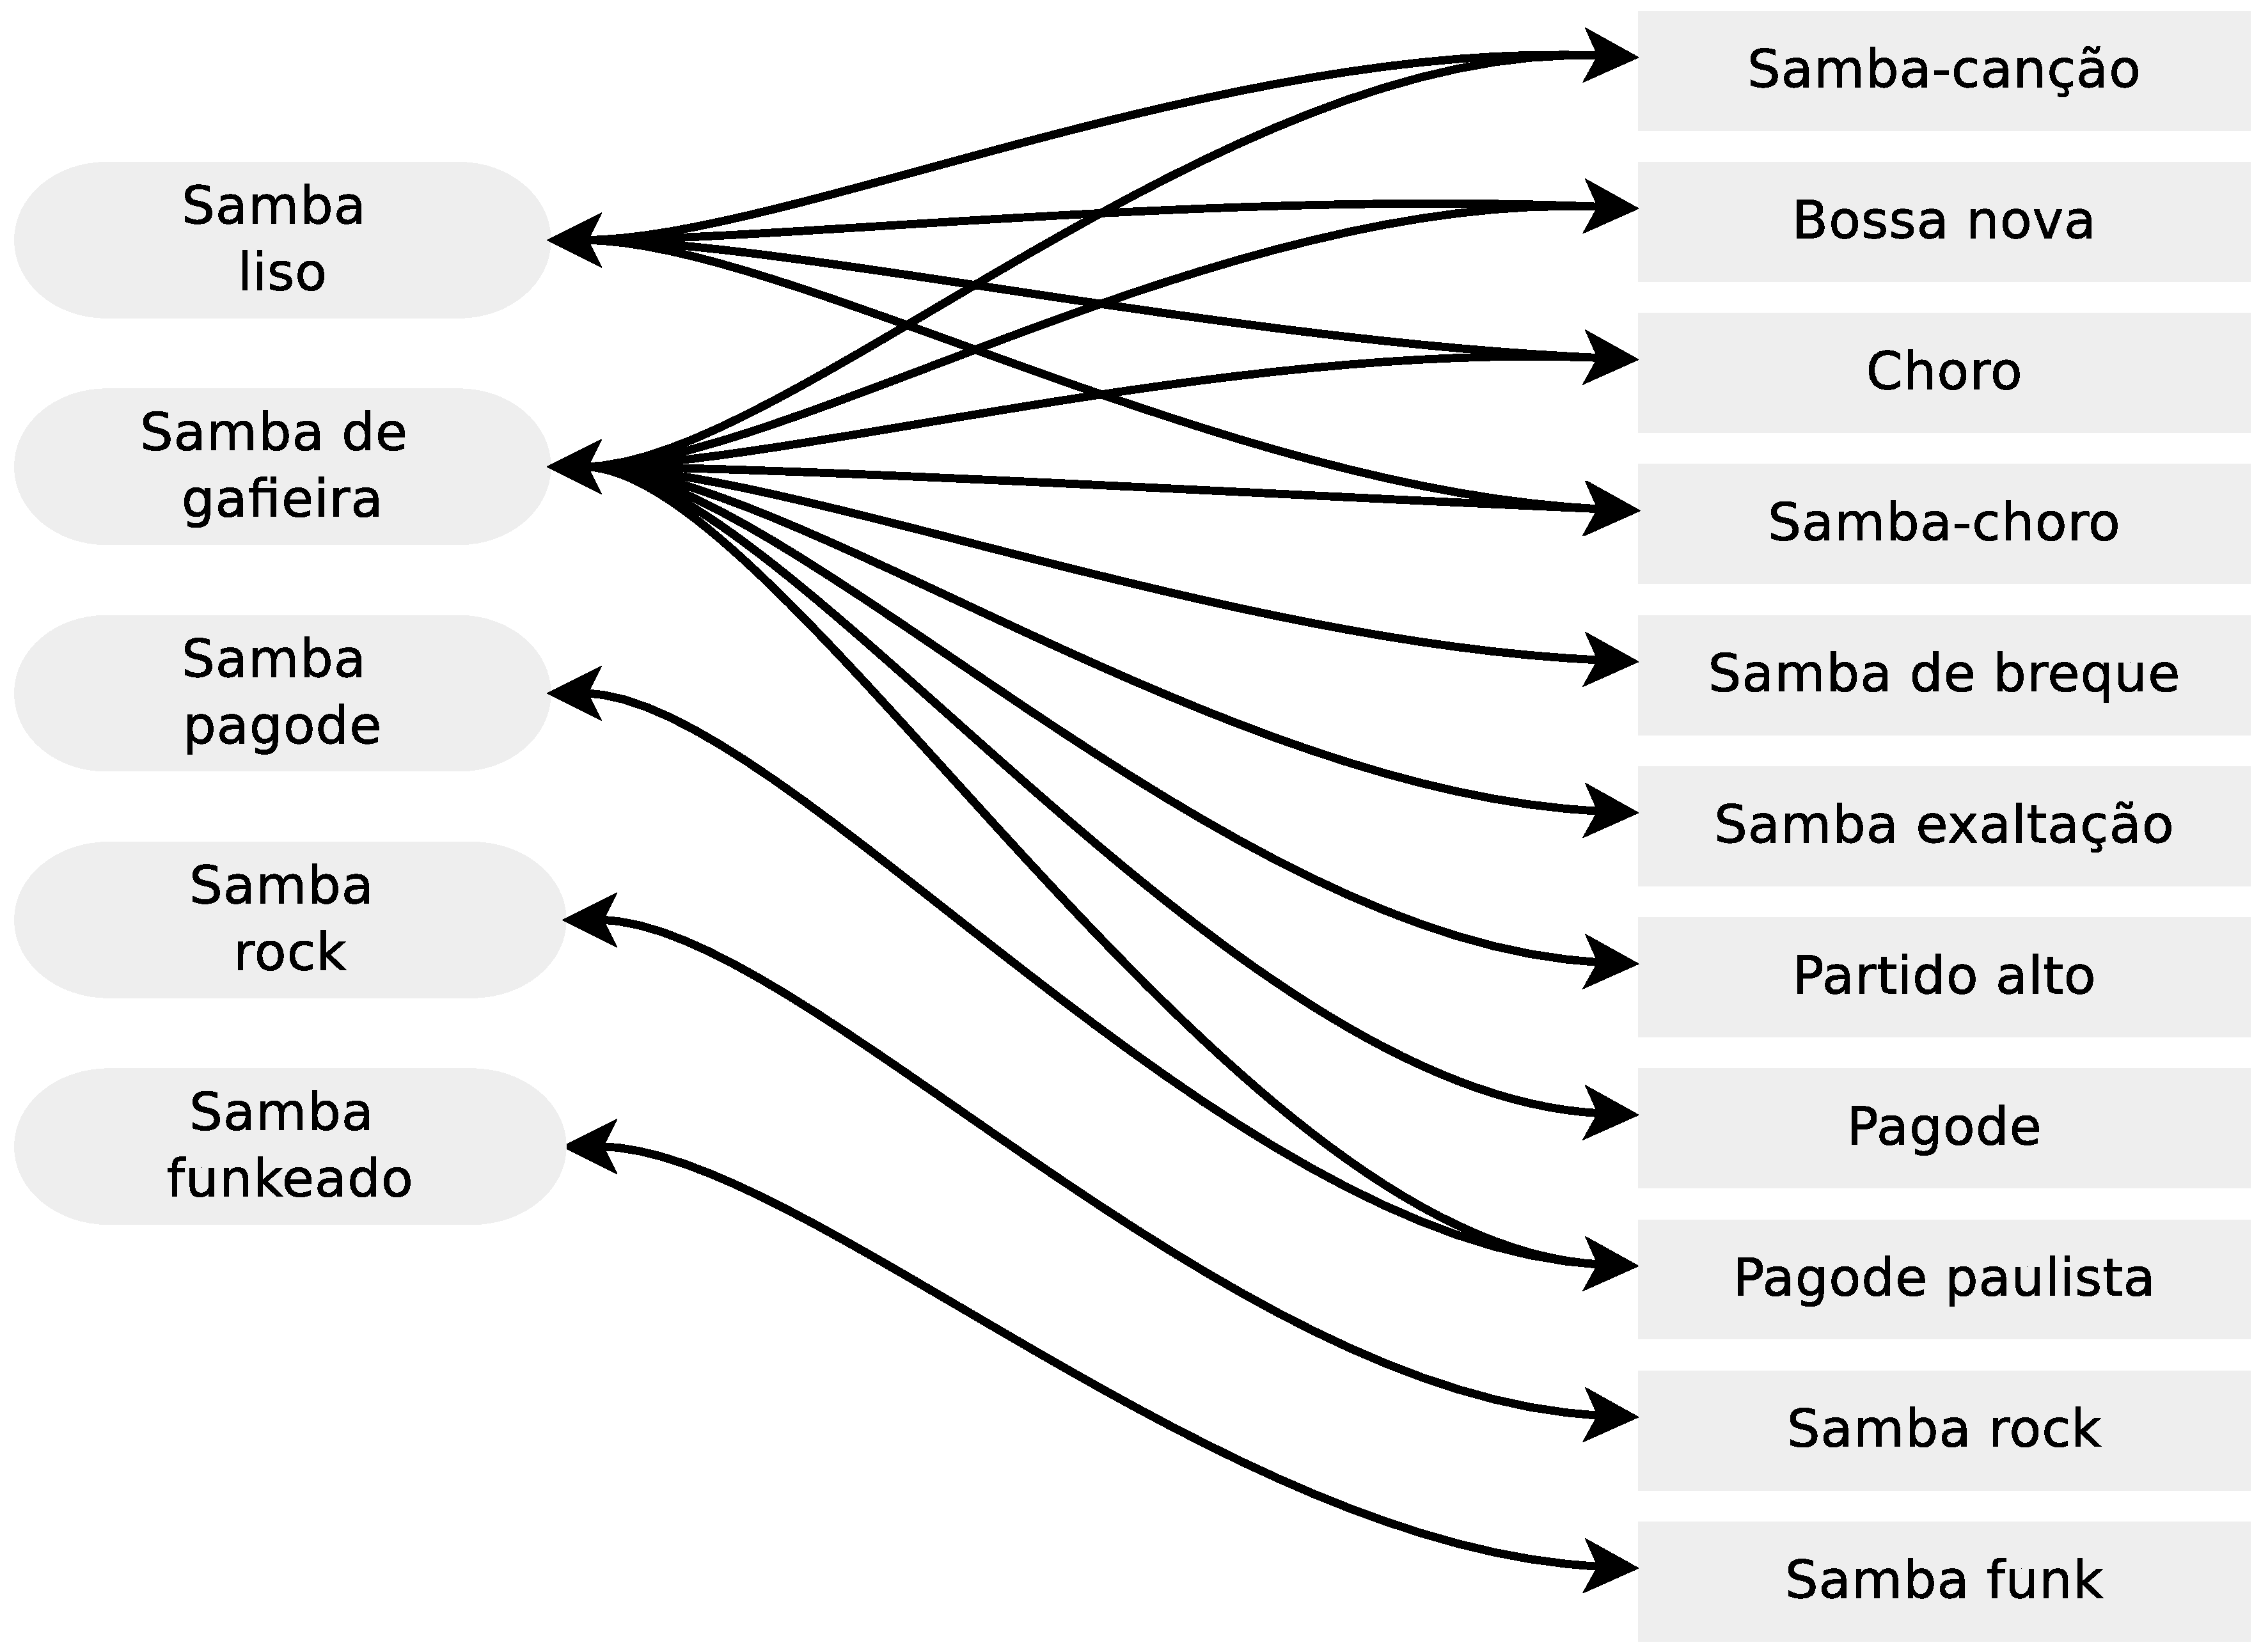
\includegraphics[width=1.0\textwidth]{chapters/cap-historia-dancasamba/dancavcmusica.eps}
  \caption{Relações entre os estilos de dança a dois e os subgêneros do samba.}
\label{fig:sambadavavsmusica}
\end{figure}

%%%%%%%%%%%%%%%%%%%%%%%%%%%%%%%%%%%%%%%%%%%%%%%%%%%%%%%%%%%%%%%%%%%%%%%%%%%%%%%%
%%%%%%%%%%%%%%%%%%%%%%%%%%%%%%%%%%%%%%%%%%%%%%%%%%%%%%%%%%%%%%%%%%%%%%%%%%%%%%%%
\section{Estilos dançados de forma separada}
Entre os estilos que se dançam de forma separada temos \cite[pp. 134]{perna2002samba}:

\subsection{Samba reggae  (dança)} 
Este estilo de samba que se dança separado, 
é uma dança baiana também conhecida como axé-dance, samba baiano ou pagode baiano,
se dança em samba reggae (música) \cite[pp. 134]{perna2002samba}.

\subsection{Samba no pé} 
É o estilo usado nas quadras das escolas de samba,
se dança bem em estilos musicais como: 
samba enredo ou em qualquer samba rápido  \cite[pp. 134]{perna2002samba}.

\subsection{Marcha de carnaval}
 É uma dança própria do carnaval para se dançar em cordões.
se dança bem em: marchas, marchas-rancho e samba-enredo lentos  \cite[pp. 135]{perna2002samba}.


\subsection{Relações entre os subgêneros do samba e os estilos dançados separadamente}

A Figura \ref{fig:sambadavavsmusicaseparado} mostra as relações existentes, 
entre os estilos de dança que se dançam separados (na esquerda) 
e alguns subgêneros do samba (na direita)  \cite[pp. 134-138]{perna2002samba}.

\begin{figure}[h]
  \centering
    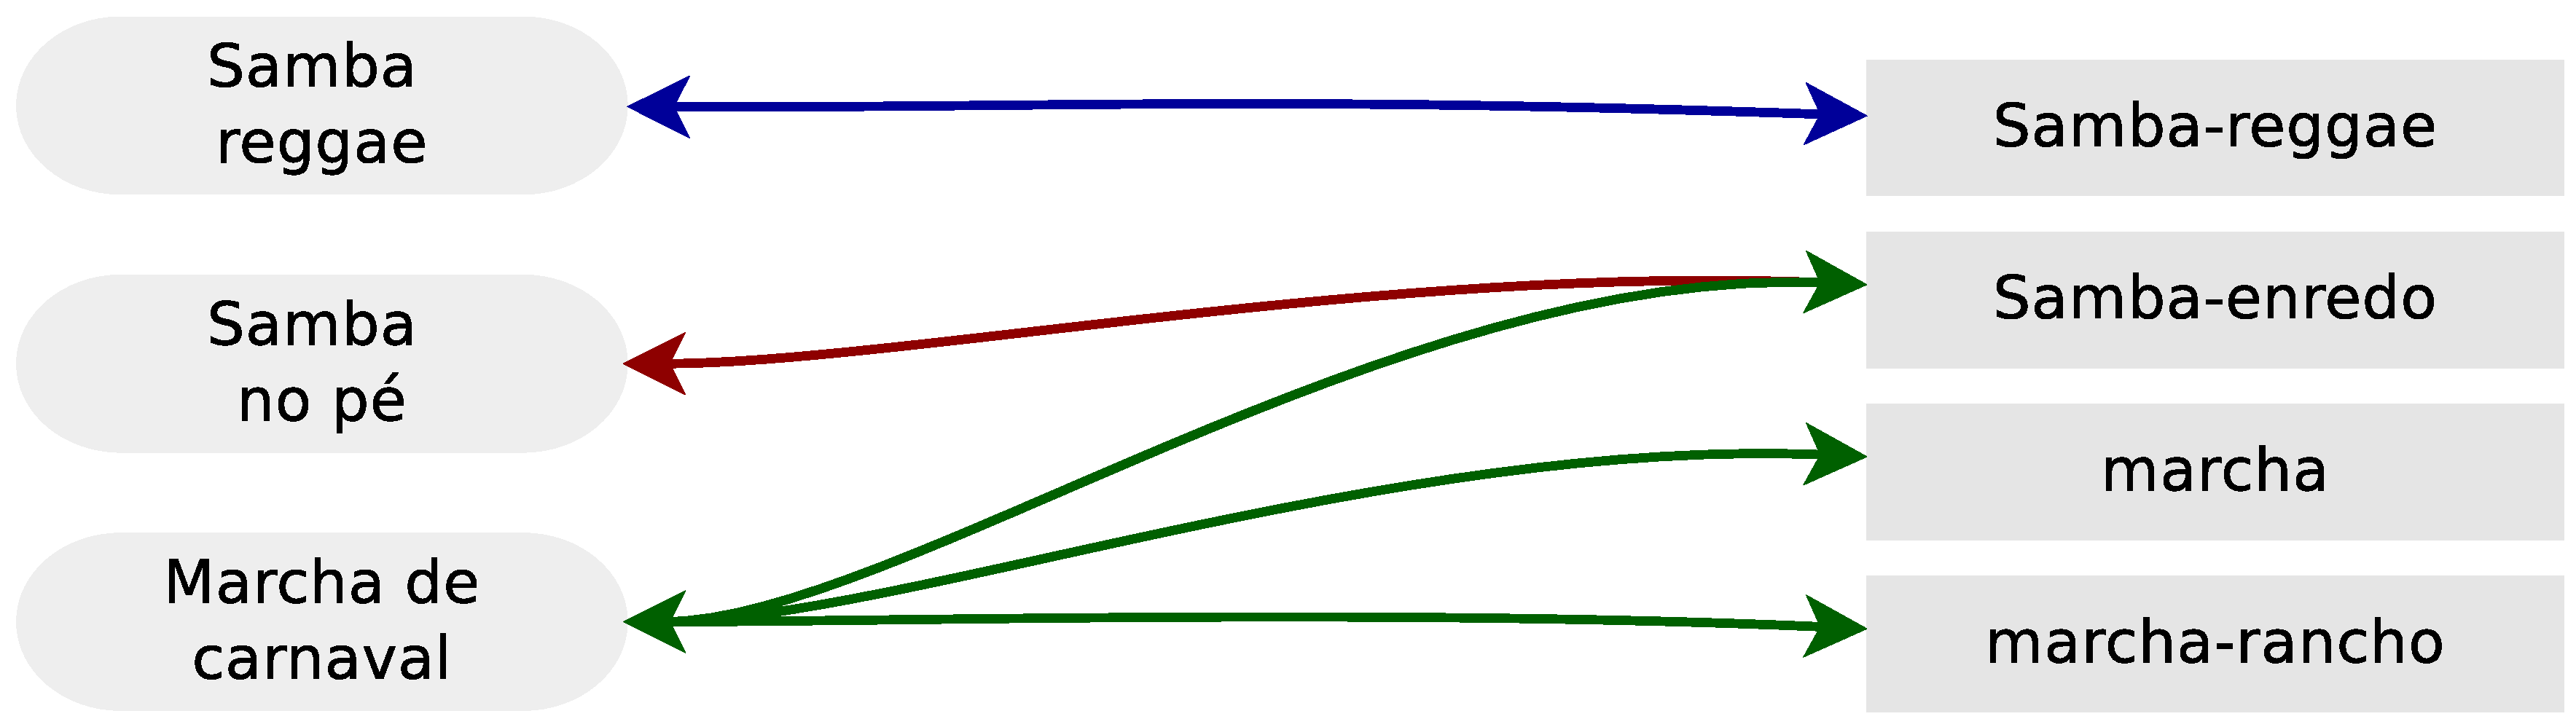
\includegraphics[width=1.0\textwidth]{chapters/cap-historia-dancasamba/dancavcmusicaseparado.eps}
  \caption{Relações entre os estilos de dança (separados) e os subgêneros do samba.}
\label{fig:sambadavavsmusicaseparado}
\end{figure}

\chapterimage{chapter_head_2.pdf} % Chapter heading image

\chapter{\textcolor{green}{Regras na dança de salão}}

\index{Regra} 
\begin{definition}[Regra:]
Norma, lei, costume que dirige, orienta e regula procedimentos (regra gramatical; regras de etiqueta; regras na dança).
[http://www.aulete.com.br/regra]
\end{definition}
\index{Condução} 
\begin{definition}[Paradigma da condução (Dança):] Este é usado na dança de salão, 
e implica que na dança a dois existe uma transmissão de informação
entre as pessoas que conformam o casal, 
de modo que a informação/comando tem um fluxo unidirecional no médio de transmissão,
que vá desde o condutor ate o seguidor. 
\end{definition}
\index{Condutor} 
\begin{definition}[Condutor (Dança):] 
A pessoa que tem o papel de conduzir e propor o movimento. 
O objetivo técnico das pessoas que optam por este rol é chegar 
a ter o sensibilidade necessária para entender onde está localizado espacialmente, 
e como distribui o peso do corpo, o seguidor; 
de modo que seja possível para o condutor aplicar uma mistura de forças e torções sobre o seguidor para provocar o movimento desejado;
chama-se a isto saber conduzir.
Sinônimos de condutor: Líder.
\end{definition}
\index{Seguidor} 
\begin{definition}[Seguidor (Dança):] 
A pessoa que recebe a condução e proporciona uma resposta corporal. 
O objetivo técnico das pessoas que optam por este rol é chegar 
a ter a sensibilidade necessária para entender as conduções,
independentemente de quem seja a pessoa que aplique a condução;
chama-se a isto ser conduzível.
Sinônimos de seguidor: Conduzido.
\end{definition}
\index{Dança social} 
\begin{definition}[Dança social:]
É uma dança com fim recreativo de prática social, não cênica, nem competitiva, 
que não tem um interesse artístico, histórico, geográfico ou técnico; 
que se universaliza e consiste em movimentos dos corpos de um casal, 
onde existe a figura condutor e o seguidor (papeis intercambiáveis) \cite{Zamoner2012} ate onde o nível técnico do par o permita.
\end{definition}
\index{Dança de salão} 
\begin{definition}[Dança de salão:]
É uma arte que procura conservar suas características técnicas, 
sua origem histórica e geográfica, e se universaliza em práticas sociais. 
Esta arte consiste na interpretação improvisada da música por médio dos movimentos 
dos corpos de um casal, utilizando um paradigma da dança onde se tem um condutor e um seguidor (papeis intercambiáveis) \cite{Zamoner2012}.
\end{definition}

Neste capítulo veremos um conjunto de regras, e a explicação de como o cumprimento
ou não destas afetam ao desenvolvimento estético e técnico da dança de 
salão\footnote{Ou na dança social sim se interessa levar estas ideias a esse âmbito.}  no paradigma da condução.

Assim, serão usados neste capítulo termos como "condutor" e "seguidor", 
mas isto não implica nenhuma obrigatoriedade ou restrição, das pessoas, para o uso de algum destes papéis na dança;
porem é comum ver que o papel de condutor é escolhido tradicionalmente pelos "cavalheiros" e o papel de seguidor pelas "damas".
%só são um recurso literário para o melhor entendimento das explicações mostradas aqui.
\begin{lattention}
É importante aclarar
que as regras expostas neste capítulo não estão regulamentadas por nenhuma entidade ou intituição; assim, estas
refletem, o meu aprendizado de distintos professores,
interpretações pessoais  e deduções. 
\end{lattention}

%%%%%%%%%%%%%%%%%%%%%%%%%%%%%%%%%%%%%%%%%%%%%%%%%%%%%%%%%%%%%%%%%%%%%%%%%%%%%%%%
\section{\textcolor{green}{Regras gerais na dança de salão}}
As regras que veremos aqui abrangem um conjunto amplo de estilos de 
dança, e não devem ser
tratadas como leis, e sim como diretrizes a serem usadas como padrão de inicialização, de modo que 
o dançarino ou dançarina analisará cada caso e se necessário criará uma exceção e atuará conforme ela.
A continuação são listadas algumas regras gerais na dança de salão.\\

\begin{itemize}
\item \textbf{Rodar o salão:} Que os dançarinos executem sua dança girando o salão, 
é importante para criar a ilusão de que o espaço de dança é maior, dado que mesmo
tendo uma pista de dança lotada, o espaço que um
casal deixa ao se movimentar é ocupado pelo casal que vem atrás deles, criando 
assim um fluxo de movimento circular que permite a todos os casais usar a pista de dança
na sua totalidade (por convenção o sentido de giro é sempre anti-horário); 
visto o anterior é importante ressaltar que né todas as danças tem
uma evolução circular na pista de dança, pois existem estilos de dança que são dançados em linha,
como por exemplo a "Salsa em linha" ou o "West coast swing", ou também existem estilos que
tem um comportamento hibrido entre circular e linha como o "Zouk". Neste sentido,
a "samba de gafieira"  tem um comportamento circular e se deveria dançar
rodando o salão para um boa etiqueta na pista de dança.
\item \textbf{Conduzir e ser conduzidos:} Trabalhar num paradigma da dança baseado
na condução é muito importante para as danças de salão, dado que isto implicará
que um condutor habilidoso poderá dançar fluidamente com pessoas com quem nunca dançou
antes (se esta for conduzível). O mesmo acontecerá para as pessoas que desenvolvam
a sensibilidade necessária para serem conduzíveis, elas poderão dançar com qualquer
condutor, inclusive poderão ter um desenvolvimento básico em estilos de dança pouco ou não conhecidos.
O caso contrario ao paradigma da condução, é ter um estilo de dança baseado em coreografias;
este enfoque, dependendo da finalidade, pode ser visto como um vicio que geralmente aparece quando iniciamos
na dança. Isto acontece, no caso do condutor, quando este assume que se realiza a parte do movimento 
que lhe corresponde (na parte visual) sem enviar nenhuma informação ao seguidor, 
este tem que reconhecer/adivinhar o movimento, e realizar a parte que lhe corresponda. Este enfoque
funciona bem quando ambos tem treinado antecipadamente os movimentos, e/ou conhecem a sequencia
em que estes movimentos serão executados, porem falha quando os dançarinos não se conhecem;
comprovar isto é fácil se imaginamos por exemplo o caso em que o condutor executa um movimento
que tem a parte inicial muito parecida a outro movimento, neste caso, se o seguidor não tiver
um poder telepático confundirá um movimento com o outro e acontecerá um problema de comunicação. Assim, a coreografia
na dança deve estar reservada para apresentações, onde o casal volta 
a sua atenção para a encenação da peça, e não para detalhes mais mecânicos.

\item \textbf{Ter o peso do corpo sobre um pé só no final da proposta de movimento:} 
Na dança de salão é muito importante a leveza e o auto controle mostrado na 
execução dos movimentos; assim, para conseguir isto, é importante que os dançarinos
tenham o peso do corpo num pé só ao terminar a execução de cada movimento; o motivo
é facilmente percebido se fazemos um pequeno exercício. Ao ficar em pé separamos as
pernas uma distancia igual à de nosso quadril, e nesse momento levamos o peso do corpo
(concentrado no nosso centro de gravidade que nesse casso está perto do umbigo) a
apontar a um ponto médio entre nossos pés, nesse instante estamos dividindo o peso do corpo
entre nossos pontos de apoio, 50$\%$ no pé direito e 50$\%$ no pé esquerdo; agora, mantendo o peso
do corpo nesse lugar, tentaremos levantar qualquer de nossos pés, será evidente
que esse trabalho é muito difícil sem perder o equilíbrio, pois para mantê-lo
precisamos de ambos pontos de apoio; casos similares podem ser vistos com qualquer proporção de distribuição de peso,
por exemplo, 30$\%$ e 70$\%$ ou 20$\%$ e 80$\%$. Assim o único caso em que estamos
equilibrados e podemos executar nosso movimento e levantar um pé 
mantendo a postura e auto controle, é quando
temos o 100$\%$ do peso do corpo num pé só, o pé de apoio. 
Por outro lado, quando consideramos ao condutor como o agente desequilibrante do seguidor, por exemplo no caso
em que este aplica uma condução;
a regra de manter o peso do corpo num pé só, tem um valor agregado; 
pois fica mais fácil para o condutor orientar
ao seguidor a fazer o seguinte movimento, dado que o único pé que este pode mover é o pé
que está livre, e que é o pé que o condutor precisa que se movimente, 
além de que a força necessária pelo condutor para tirar ao seguidor do seu equilíbrio 
atual é muito menor ao caso quando o seguidor tem dois pontos de apoio.
Adicionalmente o seguidor tem um pé livre para se resguardar do desequilíbrio provocado pelo 
condutor e adquirir um novo equilíbrio com esse pé.

\item \textbf{Ter uma abraço de dança firme:} Seguindo a ideia da condução, esta só pode
ser realizada se existe um médio de comunicação, onde possa ser transmitido
o comando do condutor ao seguidor. Assim, um bom abraço garante este
fluxo de informação.
\end{itemize}

%%%%%%%%%%%%%%%%%%%%%%%%%%%%%%%%%%%%%%%%%%%%%%%%%%%%%%%%%%%%%%%%%%%%%%%%%%%%%%%%
\section{\textcolor{blue}{Regras gerais na samba de gafieira}}


\begin{itemize}
\item \textbf{Quadril avança, ombros e pé acompanham}  O movimento inicia no quadril.
\item \textbf{Quando movimentar um pé chegar com 100$\%$ do peso do corpo} estética da samba de gafieira.
\item \textbf{Braços firmes do seguidor} estes transportam a informação para o quadril (ex: picadilho).
\item \textbf{Abraço uniforme do condutor} este procura manter a mesma distancia (ex: gancho redondo).
\item \textbf{O tórax do condutor guia ao seguidor} O tórax do condutor guia ao seguidor (NÃO o braço).
\item \textbf{Procurar o paralelismo de ombros e linha de visão do casal} é responsabilidade do seguidor seguir ao condutor, indução.
\item \textbf{O pé de apoio debe estar apontando a um ponto médio entre os pês do par de dança} .
\end{itemize}


%%%%%%%%%%%%%%%%%%%%%%%%%%%%%%%%%%%%%%%%%%%%%%%%%%%%%%%%%%%%%%%%%%%%%%%%%%%%%%%%
%% CAPITULO
%%%%%%%%%%%%%%%%%%%%%%%%%%%%%%%%%%%%%%%%%%%%%%%%%%%%%%%%%%%%%%%%%%%%%%%%%%%%%%%%
\chapterimage{chapter_head_2.pdf} % Chapter heading image

%%%%%%%%%%%%%%%%%%%%%%%%%%%%%%%%%%%%%%%%%%%%%%%%%%%%%%%%%%%%%%%%%%%%%%%%%%%%%%%
%%%%%%%%%%%%%%%%%%%%%%%%%%%%%%%%%%%%%%%%%%%%%%%%%%%%%%%%%%%%%%%%%%%%%%%%%%%%%%%
%%%%%%%%%%%%%%%%%%%%%%%%%%%%%%%%%%%%%%%%%%%%%%%%%%%%%%%%%%%%%%%%%%%%%%%%%%%%%%%
%%%%%%%%%%%%%%%%%%%%%%%%%%%%%%%%%%%%%%%%%%%%%%%%%%%%%%%%%%%%%%%%%%%%%%%%%%%%%%%
\chapter{\textcolor{blue}{Passos do samba de gafieira}}
%\index{Passos}

\begin{definition}[Plano axial:] 
\index{Plano axial}
\label{def:PlanoAxial}
O Dicionário Priberam da Língua Portuguesa \cite{priberamplano} define plano axial como:
Plano transversal, plano horizontal que divide o corpo ou uma estrutura anatômica em parte superior e parte inferior.
Ver Figura \ref{fig:bodyhumanplane}.
\end{definition}

\begin{definition}[Plano frontal:] 
\index{Plano frontal}
\label{def:PlanoFrontal}
O Dicionário Priberam da Língua Portuguesa \cite{priberamplano} define plano frontal como:
Plano coronal,   plano vertical e paralelo à sutura coronal do crânio, que divide o corpo em parte anterior e parte posterior.
Ver Figura \ref{fig:bodyhumanplane}.
\end{definition}

\begin{definition}[Plano sagital:] 
\index{Plano sagital}
\label{def:PlanoSagital}
O Dicionário Priberam da Língua Portuguesa \cite{priberamplano} define plano sagital como:
Plano vertical e paralelo à sutura sagital do crânio, que divide o corpo em parte direita e parte esquerda.
Ver Figura \ref{fig:bodyhumanplane}.
\end{definition}

\begin{figure}[h!]
  \centering
    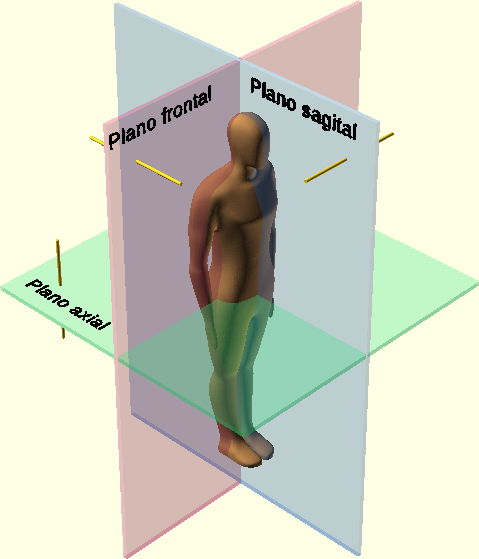
\includegraphics[width=0.60\textwidth]{body-plane/files/body-plane.png}
  \caption{ Planos e eixos no corpo humano.}
\label{fig:bodyhumanplane}
\end{figure}

\begin{definition}[Eixo axial:] 
\index{Eixo axial}
\label{def:EixoAxial}
É o eixo perpendicular ao plano axial.
Ver Figura \ref{fig:bodyhumanplane}.
\end{definition}

\begin{definition}[Eixo frontal:] 
\index{Eixo frontal}
\label{def:EixoFrontal}
É o eixo perpendicular ao plano frontal.
Ver Figura \ref{fig:bodyhumanplane}.
\end{definition}

\begin{definition}[Eixo sagital:] 
\index{Eixo sagital}
\label{def:EixoSagital}
É o eixo perpendicular ao plano sagital.
Ver Figura \ref{fig:bodyhumanplane}.
\end{definition}

\begin{definition}[Passo cíclico:] 
\index{Passo cíclico}
\label{def:PassoCiclico}
É um passo de dança que pode acontecer por um tempo indeterminado,
devido a que este está composto por ciclos, cuja postura de inicio e final é a mesma.
\end{definition}

\begin{definition}[Passo simétrico:] 
\index{Passo simétrico}
\label{def:PassoSimetrico}
É um passo de dança que tem a primeira metade do passo similar à segunda,
com a diferencia que se executa com os pés intercambiado (direita por esquerda)
ou com as posições dos corpos intercambiadas (seguidor por condutor).
\end{definition}

\begin{definition}[Duração do movimento:] 
\index{Duração do movimento}
\label{def:DuracaoDoPasso}
Ou a \textbf{duração do passo}, 
é a longitude temporal de um passo de dança, contado em tempos da música.
No caso de \hyperref[def:PassoCiclico]{\textbf{passos cíclicos}}, a duração do passo se refere a duração do ciclo.
\end{definition}


\begin{definition}[Dançar no tempo forte:] 
\index{Dançar no tempo forte}
\label{def:DancaNoTempo}
Ou simplesmente \textbf{dançar no tempo}, indica que se está dançando com passos com o movimento principal ou inicial (dependendo do estilo de dança), 
se executando no tempo forte da música; ver Exemplo \ref{example:dancatempoforte}.
\end{definition}
\begin{example}
\label{example:dancatempoforte}
Se definimos um passo de dança como: Pisar, usando um pé cada vez, 
realizando um movimento com uma distribuição espacial, junto-junto-longo;
e definimos ao movimento ``longo'' como o movimento principal. 
Se executássemos o movimento ``longo'' no tempo forte, o passo junto-junto-longo,
estaria sendo dançado no tempo forte.
\end{example}

\begin{definition}[Dançar em contratempo:] 
\index{Dançar no contratempo}
\label{def:DancaNoContratempo}
Indica que se está dançando, com o movimento principal ou inicial (dependendo do estilo de dança) do passo, 
executando-se em contra do tempo forte da música; é dizer, executando-se num tempo fraco (em contratempo).
Com diferencia de \hyperref[def:DancaNoTempo]{\textbf{dançar no tempo forte}}, 
que é único, pois só existe um tempo forte;
existem varias formas de dançar como o movimento principal em algum tempo fraco; ver Exemplo \ref{example:dancatempofraco}.
\end{definition}
\begin{example}
\label{example:dancatempofraco}
Se definimos um passo de dança como: Pisar, usando um pé cada vez, 
realizando um movimento com uma distribuição espacial, junto-junto-longo;
e definimos ao primeiro movimento ``junto'' como o movimento principal. 
Se executássemos o movimento ``longo'' no tempo forte, o passo junto-junto-longo,
estaria sendo dançado em contratempo.
\end{example}

\begin{definition}[Passo a contratempo:] 
\index{Passo a contratempo}
\label{def:PassoAContratempo}
É um passo de dança cuja execução promove que quando se esteja dançando com um pé especifico acompanhando o tempo forte da música,
ao finalizar o passo este pé esteja sendo marcado no tempo fraco.
É dizer, são movimento onde após de realizados, 
passamos de \hyperref[def:DancaNoTempo]{\textbf{dançar no tempo}} a 
\hyperref[def:DancaNoContratempo]{\textbf{dançar no contratempo}} e vice-versa. 
No samba de gafieira, isto acontece quando o número de tempos musicais que o passo  usa é impar;
pois as músicas tradicionalmente são escritas sombre compassos binários, 
pelo que comumente acharemos um tempo forte intercalado por uno tempo fraco.
\end{definition}

\begin{definition}[Passo de deslocamento:] 
\index{Passo de deslocamento}
\label{def:PassoDeDeslocamento}
É um passo de dança cujo propósito, consequência ou objetivo é o deslocamento no salão.
\end{definition}

\begin{definition}[Postura de finalização:] 
\index{Postura, tipos!Postura de finalização}
\label{def:PosturaFinaliza}
É uma postura a qual da a percepção, 
de que se tem chegado ao ponto final da ideia expressada com o movimento.
Se nossa dança fosse um relato escrito, esta postura seria equivalente a um ponto ou ponto e virgula.
\end{definition}

\begin{definition}[Postura de transição:] 
\index{Postura, tipos!Postura de transição}
\label{def:PosturaTransicao}
É uma postura a qual da a percepção, 
de que não se tem completado a ideia expressada com o movimento, e que possivelmente vem mais algum outro movimento.
Se nossa dança fosse um relato escrito, esta postura seria equivalente a uma virgula ou espaço em branco entre as palavras.
\end{definition}


%%%%%%%%%%%%%%%%%%%%%%%%%%%%%%%%%%%%%%%%%%%%%%%%%%%%%%%%%%%%%%%%%%%%%%%%%%%%%%%
%%%%%%%%%%%%%%%%%%%%%%%%%%%%%%%%%%%%%%%%%%%%%%%%%%%%%%%%%%%%%%%%%%%%%%%%%%%%%%%
%%%%%%%%%%%%%%%%%%%%%%%%%%%%%%%%%%%%%%%%%%%%%%%%%%%%%%%%%%%%%%%%%%%%%%%%%%%%%%%
\section{\textcolor{blue}{Que passos existem no samba de gafieira?}}

No ano \AnoLivro~ podemos ver uma grande variedade de passos para o samba de gafieira,
tantos como a imaginação possa atingir, pois além dos movimentos mais conhecidos e  consagrados da dança,
podem existir variações  destes ou simplesmente estilos em que estos são realizados. 



Nas seguintes subseções, listaremos e descreveremos 
alguns dos passos que são possíveis de ver no samba de gafieira;
mas, estas descrições não pretendem ser uma guia de ensino,
e sim um instrumento para saciar a curiosidade do leitor em como os movimentos são realizados.\\

%%%%%%%%%%%%%%%%%%%%%%%%%%%%%%%%%%%%%%%%%%%%%%%%%%%%%%%%%%%%%%%%%%%%%%%%%%%%%%%
%%%%%%%%%%%%%%%%%%%%%%%%%%%%%%%%%%%%%%%%%%%%%%%%%%%%%%%%%%%%%%%%%%%%%%%%%%%%%%%
\PRLsep{Passos no samba de gafieira ate 1949}

%%%%%%%%%%%%%%%%%%%%%%%%%%%%%%%%%%%%%%%%%%%%%%%%%%%%%%%%%%%%%%%%%%%%%%%%%%%%%%%
\subsection{Balão} 
\label{def:PassoBalao}
\index{Passo!Balão}
\index{Passo a contratempo!Balão}
%%                CICLICO    |SIMETRICO   |CONTRATEMPO   |DESLOCAMENTOS |TIEMPOS
\caracterpasso{\NoCheckedItem}{\NoCheckedItem}{\CheckedItem}{\NoCheckedItem}{3}
Um movimento com este nome já existia desde as origens do samba nas gafieiras, 
sendo este movimento proveniente do maxixe \cite[pp. 142]{perna2002samba} 
\cite[pp. 93]{efege1974maxixe} \cite[pp. 465]{marcondes1977enciclopedia}.
%porem não tem se achado referencias sobre as caraterísticas do movimento no maxixe.



Seguindo o Prof. Gino Fornaciari, no ano 1947,  em São Paulo, se usava o nome balão e pião,
para representar a um mesmo movimento, um que agora chamaríamos de pião, 
porem o pião de 1947 era em sentido anti-horário \cite[pp. 68-72]{fornaciari1947aprender}.
Por outro lado, no seu livro ``Como apender a dançar'' (1950) 4ta edição,
o Prof. Fornaciari descreve um movimento  chamado ``Calçada'', com uma descrição semelhante 
ao ``balão'' de \AnoLivro~ \cite[pp. 162]{fornaciari1950aprender}.

Em \AnoLivro, o nome balão designa a um movimento que pode ser considerado aéreo, 
pois o \hyperref[def:Condutor]{\textbf{condutor}} tira do chão os pés do \hyperref[def:Seguidor]{\textbf{seguidor}}.
Um movimento com estas caraterísticas pode ser visto no filme ``Aviso aos navegantes'' (1950),
pelo que podemos especular que este era de uso comum desde muito antes \cite[min. 40:35]{AtlantidaDance};
porem, não pode-se souber sim lhe era atribuído ou não nessa época o nome de balão; 
mas pela semelhança com o movimento de quadril do passo chamado balão apagado,
é provável que sim, 
pois lembremos que o problema da homologação da nomenclatura dos passos existe ate em  nossos dias.



O movimento dura 3 tempos, o passo inicia com o seguidor ao lado direito do condutor, 
ligeiramente atrás dele, com um \hyperref[def:abracodedanca]{\textbf{abraço de dança}} 
bem próximo e uma postura similar a postura de X só que com os pés mais juntos.
No primeiro tempo o condutor da um passo ao lado, e pisa com o pé direito,
de modo que o seguidor fique em pé atrás da perna direita do condutor, sem perder o abraço.
No segundo tempo, aproveitando a postura, 
o condutor faz um movimento circular anti-horário com seu quadril, no \hyperref[def:PlanoAxial]{\textbf{plano axial}},
de modo que sua perna direita, que está em contato com a perna direita do seguidor,
serva como alavanca para tirar ao seguidor do chão, 
e este gire ou voe ao redor \footnote{O giro do seguidor é com o corpo reto e pernas juntas, 
como se fosse uma fita solta de um lado e com o outro lado presso num ponto 
que provoca o giro da fita no \hyperref[def:PlanoAxial]{\textbf{plano axial}}, com giro ao redor do eixo axial.} 
do condutor em sentido anti-horário.
No terceiro tempo o seguidor senta-se, é dizer faz uma cadeirinha, sobre a perna esquerda do condutor,
que para receber ao seguidor  da um passo ao frente.

\begin{comment}
A Figura \ref{fig:balao1950} mostra um fotograma do filme ``Aviso aos navegantes'' (1950),
onde se observa o inicio do passo balão (\AnoLivro), quando a moça tira os pés do chão.
\begin{figure}[h!]
  \centering
    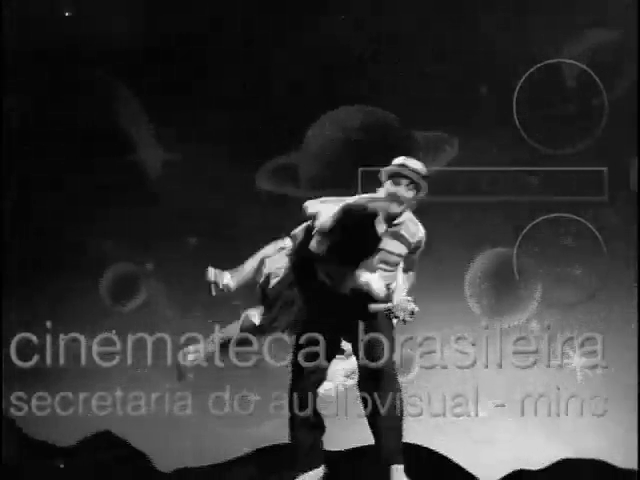
\includegraphics[width=0.7\textwidth]{chapters/cap-historia-passos/balao1950.png}
  \caption{Fotograma com o inicio do passo balão (\AnoLivro), do filme ``Aviso aos navegantes'' (1950) \cite[min. 40:35]{AtlantidaDance}.}
  \label{fig:balao1950}
\end{figure} 
\end{comment}

%%%%%%%%%%%%%%%%%%%%%%%%%%%%%%%%%%%%%%%%%%%%%%%%%%%%%%%%%%%%%%%%%%%%%%%%%%%%%%%
\subsection{Balão apagado}
\index{Passo!Balão apagado} 
\index{Passo cíclico!Balão apagado}
\index{Passo simétrico!Balão apagado}
%%                CICLICO     |SIMETRICO   |CONTRATEMPO   |DESLOCAMENTOS |TIEMPOS
\caracterpasso{\CheckedItem}{\CheckedItem}{\NoCheckedItem}{\NoCheckedItem}{4}
Um movimento com este nome já existia desde as origens do samba nas gafieiras, 
sendo este movimento proveniente do maxixe \cite[pp. 142]{perna2002samba} \cite[pp. 68]{efege1974maxixe}.
Um exemplo do movimento que agora designamos como balão apagado pode 
ser visto no filme ``Aviso aos navegantes'' (1950) \cite[min. 40:35]{AtlantidaDance}.
\begin{comment}
A Figura \ref{fig:balaoapagado1950} mostra um fotograma do filme onde se observa o movimento de quadril no balão apagado.
\begin{figure}[h!]
  \centering
    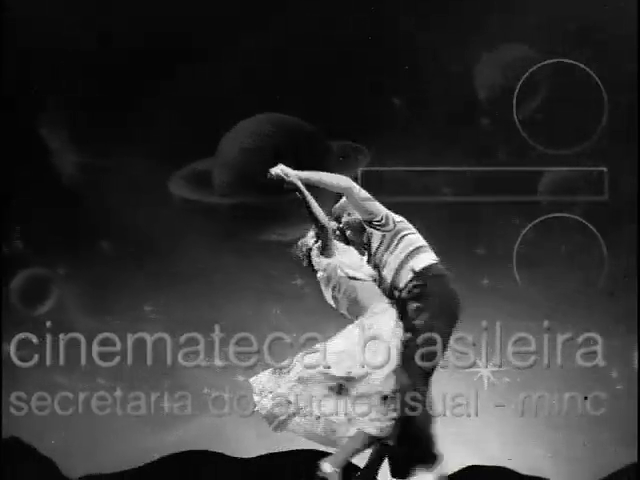
\includegraphics[width=0.7\textwidth]{chapters/cap-historia-passos/balaoapagado1950.png}
  \caption{Fotograma que mostra a execução do passo balão apagado, tirado do filme ``Aviso aos navegantes'' (1950) \cite[min. 40:35]{AtlantidaDance}.}
  \label{fig:balaoapagado1950}
\end{figure}
\end{comment}

Em \AnoLivro, este movimento tem um parecido ou lembrança com o \hyperref[def:PassoBalao]{\textbf{balão}} (\AnoLivro); 
porem, se realiza com o par num \hyperref[def:abracodedanca]{\textbf{abraço de dança}} estando um frente ao outro, 
consequentemente o \hyperref[def:Seguidor]{\textbf{seguidor}} não voa ao redor do \hyperref[def:Condutor]{\textbf{condutor}}, 
se não que a intenção de voar se apaga e o seguidor nunca sai do chão; 
de modo que o casal fica dando giros, abraçados, num eixo comum e praticamente no lugar. 
Estes giros são promovidos por marcados movimentos circulares de quadril, que mudam
de velocidade e intenção num constante, abrupto, leve e leve,  na proporção de tempos \{1/2 tempo,1/2 tempo, tempo\}; 
semelhando assim ao movimento de um balão perdendo o ar.
Existem variantes deste movimento, onde o giro do par é realizado em sentido horário e anti-horário; porem, 
não saberia afirmar qual é a versão padrão; mas, pelas minhas observações a versão mais difundida,
é a que faz o giro em sentido anti-horário.

Este movimento é um \hyperref[def:PassoCiclico]{\textbf{passo cíclico}}, com ciclos que duram 4 tempos, 
sendo o primeiro par de tempos similar ao segundo, porem com os papeis intercambiados no par de dança.
No momento inicial, o casal está abraçado numa postura frente a frente, 
com o peso do corpo do lado da perna direita do condutor;
no tempo 1 o condutor da um passo e pisa com a perna esquerda pra traz, 
como se procura-se ocultar esta atrás da sua perna direita, 
este movimento de perna é promovido pelo movimento circular do 
quadril em sentido anti-horário no \hyperref[def:PlanoAxial]{\textbf{plano axial}};
por outro lado, 
o seguidor da um passo adiante com sua perna direita procurando manter a postura 
relativa com o condutor e acompanhando o movimento circular anti-horário do quadril, 
de modo que se seu pé direito tende a   rodear ao condutor.
Nos tempos 1.5 e 2 o par pisa no lugar, ajeitando suas posturas apagando o movimento do quadril, 
mas mantendo o giro do par, 
de modo que terminam abraçados  frente a frente com o peso do corpo no lado do pé esquerdo do condutor.
No próximo par de tempos, o movimento é similar, só que agora é o seguidor que inicia dando um passo com o pé esquerdo. 

%%%%%%%%%%%%%%%%%%%%%%%%%%%%%%%%%%%%%%%%%%%%%%%%%%%%%%%%%%%%%%%%%%%%%%%%%%%%%%%
\subsection{Puladinho }
\index{Passo!Puladinho}
\index{Passo cíclico!Puladinho}
\index{Passo simétrico!Puladinho}
\index{Passo de deslocamento!Puladinho}
\begin{comment} 
neste movimento não se pula; 
existem varias referencias não acadêmicas na internet, que datam desde o 2002,
onde não mencionam ao ``Puladinho'' e sim um passo chamado ``pruladinho'', 
pelo qual suspeito que este faz referencia ao mesmo passo;
pois indica corretamente que no movimento se vá ``pra o ladinho''.
\end{comment}
%%                CICLICO     |SIMETRICO   |CONTRATEMPO   |DESLOCAMENTOS |TIEMPOS
\caracterpasso{\CheckedItem}{\CheckedItem}{\NoCheckedItem}{\CheckedItem}{4}
Na polca, trazida ao Brasil em 1845, 
existia um movimento chamado puladinho,
que era um movimento que se fazia sobre as pontas dos pés,
indo para adiante, iniciando com o pé esquerdo estacando obliquamente à esquerda,
num segundo momento o pé direito avança ate ficar junto ao outro, 
para logo deslizar o pé esquerdo para adiante, 
permitindo assim levantar o pé direito para ajeitar a postura 
e recomeçar o movimento com esquerdo \cite[pp. 58-59]{tinhorao1986pequena}.
É fácil perceber que este movimento tem alguns pontos semelhantes ao puladinho (\AnoLivro),
no fato do andar oblíquo e a troca de pesos, porem o puladinho da polca não era simétrico para ambos pés.

Por outro lado, no maxixe (dança)  que é descrito em 1920 na ``Revista do Brasil'',
se mencionam os termos maxixe ``puladinho'' e maxixe de ``esquentar a barriga'',
como descrições usadas pelos aficionados a esta dança, 
pelo que se entende que no maxixe também existiu um movimento chamado puladinho \cite[pp. 177]{1920revista}. 

Adicionalmente, no livro ``Oito décadas: memórias'', se menciona que na década de
1920 existia uma variante do samba que se chamava ``o puladinho'' 
que introduziu nos salões o carnaval do povo, 
e que provocava entre as jovens da época, em palavras da autora, 
``a externalização da sensualidade reprimida'' \cite[pp. 94-95]{nabuco2000oito}.

Conhecidas estas informações, é importante lembrar que a polca influenciou a criação do maxixe (dança), 
que a sua vez influenciou a criação do samba dançado nas gafieiras,
que se condensou no samba de gafieira (\AnoLivro), o qual tem em nossos dias um passo chamado puladinho. 
Pelo que pode-se considerar, pela existência do termo em todas as evoluções da dança; 
que um movimento chamado puladinho 
já estava também presente nos primeiros sambas dançados nas gafieiras. 

Reforçando esta hipótese, podemos achar uma referencia ao uso do termo puladinho, no título de uma música instrumental chamada 
``Puladinho na gafieira'' (1958)  de  Marisa com Moacyr Silva e seu conjunto: Convite à música \cite{puladinhogafieiramusic}.
Também, podemos ver uma menção a este movimento, junto a outros conhecidos no samba de gafieira,
em 1976 na revista ``Veja'' \cite[pp. 158]{1976veja},
em 1978 na letra da canção ``Baile no Elite'' \cite{BaileNoElite} e 
em 1979 na revista ``Isto é'' \cite[pp. 89]{revista1979isto}.



Finalmente, podemos ver uma referencia a esse passo de dança, no ``jornal dos sports''(RJ),
do dia 17 de julho de 1986 \cite[pp. 6]{gafieiraaredeout2}.


O puladinho, de \AnoLivro, é executado com o casal abraçado frente a frente, sendo este um \hyperref[def:PassoCiclico]{\textbf{passo cíclico}},
com uma duração de 4 tempos; onde o movimento dos dois primeiros tempos
é simétrico ao segundo par de tempos.
Desde o ponto de vista do  \hyperref[def:Condutor]{\textbf{condutor}}, 
este inicia o movimento levando o peso do corpo junto com seu pé direito para atrás, provocando que
o \hyperref[def:Seguidor]{\textbf{seguidor}} de um passo ao frente acompanhando-lhe;
porem o condutor realiza seu movimento predominantemente pela ação do quadril e com um ligeiro arco para a direita, 
com o fim de dar molejo ao movimento;
no tempo 1.5 sem deslocar os pés, 
se faz uma troca de peso do corpo para o pé esquerdo do condutor (direito do seguidor) usando o quadril,
e finalmente no tempo 2 o condutor volta a levar o peso 
do corpo para a sua perna direita (esquerdo do seguidor) novamente usando o quadril.
Neste ponto a metade do ciclo foi realizado e o movimento se repete simetricamente, 
de modo que no tempo 3 o condutor leva atrás o seu pé esquerdo (direito do seguidor) e continua em 3.5 e 4.

 
%%%%%%%%%%%%%%%%%%%%%%%%%%%%%%%%%%%%%%%%%%%%%%%%%%%%%%%%%%%%%%%%%%%%%%%%%%%%%%%
\subsection{Pião}
\index{Passo!Pião}
\index{Passo cíclico!Pião}
\index{Passo simétrico!Pião}
\index{Passo de deslocamento!Pião}

Seguindo o Prof. Gino Fornaciari, no ano 1947,  em São Paulo, os nomes pião e balão,
representavam ao mesmo movimento, no samba-batucada\footnote{Samba de gafieira primigeinio.}; 
porem o pião de 1947 era em sentido anti-horario \cite[pp. 68-72]{fornaciari1947aprender}.
Também, podemos ver uma menção a este movimento, junto a outros conhecidos no samba de gafieira, 
em 1979 na revista ``Isto é'' \cite[pp. 89]{revista1979isto}.
Todas estas afirmações são coerentes com as declarações de Jimmy de Oliveira 
que indica que o pião já existiam antes do 1990 \cite{sambafunkeadoJimmyDeOliveiraPart1}.

%%                CICLICO     |SIMETRICO   |CONTRATEMPO   |DESLOCAMENTOS |TIEMPOS
\caracterpasso{\CheckedItem}{\CheckedItem}{\NoCheckedItem}{\CheckedItem}{4}
O pião, de \AnoLivro, é um \hyperref[def:PassoCiclico]{\textbf{passo cíclico}} que é executado com o casal abraçado, 
realizando giros sobre um eixo comum.
Cada giro dura 2 tempos, e é realizado tradicionalmente em sentido horário;
na primeira metade do giro (que dura 1 tempo) o eixo de giro do par é colocado sobre uma pessoa do par, 
de modo que a outra pessoa gira ao redor (em 1 tempo), ate chegar a uma postura similar à inicial, 
porem com os papeis intercambiadas no par, com respeito ao tempo anterior;
na outra metade do ciclo se repete o movimento, porem agora é a outra pessoa que terá o eixo do par.
Este é um movimento de deslocamento, de modo que se procura girar movimentando-se numa linha reta.

%%%%%%%%%%%%%%%%%%%%%%%%%%%%%%%%%%%%%%%%%%%%%%%%%%%%%%%%%%%%%%%%%%%%%%%%%%%%%%%
\subsection{Pica-pau} 
\index{Passo!Pica-pau}
\index{Passo cíclico!Pica-pau}
\index{Passo simétrico!Pica-pau}

%%                CICLICO     |SIMETRICO   |CONTRATEMPO   |DESLOCAMENTOS |TIEMPOS
\caracterpasso{\CheckedItem}{\CheckedItem}{\NoCheckedItem}{\NoCheckedItem}{4}
Nos primórdios do samba nas gafieiras existia um passo de dança com esse nome \cite[pp. 142]{perna2002samba}.
No Fandango\footnote{Para mais informação sobre o fandango, ir a Pag. \pageref{fig:fandango}.} 
rufado-bailado de São Paulo, em 1948, existiu uma dança chamada ``pica-pau'';
%com uma coreografia semelhante ao ``anucorrido'' (anu-corrido);
em Itanhaém (SP) esta dança é caraterizada por pares espalhados no salão,
onde o canto do violeiro é alternado com batidas de pé e palmas pelos 
cavalheiros \cite[pp. 607-608]{marcondes1977enciclopediav2} \cite[pp. 49]{fandangoSP},
esta caraterística do uso dos pés é o que da uma semelhança ao pica-pau do samba de gafieira (\AnoLivro),
que leva esse nome porque se bate o chão com a ponta (ou meia ponta) do pé simulando as bicadas de um pássaro pica-pau.
Porem, a existência do pica-pau no fandango não indica uma relação de vinculo parental do movimento,
e sim que no consciente coletivo, o estilo de imitar ao pica-pau, na dança,
já estava presente desde antes dessa época.
Um movimento com as caraterísticas do pica-pau (\AnoLivro) pode ser visto 
no filme ``Aviso aos navegantes'' (1950) \cite[min. 40:35]{AtlantidaDance}.


No \AnoLivro, o passo pica-pau, é um \hyperref[def:PassoCiclico]{\textbf{passo cíclico}} que dura 4 tempos, 
sendo os dois primeiros simétricos aos dois últimos, 
onde no primeiro par de tempos se usa só um pé,
e no segundo o outro.
Se iniciamos com o peso do corpo na perna esquerda, 
no tempo 1 marcamos com o pé direito, um pouco atrás do pé esquerdo, 
com a ponta ou meia ponta do pé e sem levar o peso,
no tempo 1.5 repetimos o mesmo movimento com o mesmo pé, e finalmente
no tempo 2 colocamos o pé direito ao lado e a direita do pé esquerdo, 
levando esta vez o peso do corpo. 
Nos tempo 3, 3.5 e 4 se repete o movimento explicado anteriormente; porem,
agora se usa o pé esquerdo.
  
\begin{figure}[t]
\begin{elaboracion}[title=Fandango]

Esta é a designação que se lhe dá a todas as danças de 
roda para adultos, em São Paulo, Paraná, Santa Catarina e Rio Grande do Sul;
este termo para eles significa baile rural ou popular \cite[pp. 261]{marcondes1977enciclopedia}.
No litoral paulista, em 1948, o Fandango é dividido principalmente em duas categorias: Fandango rufado, 
e Fandango bailado (ou valsado), porem existe a possibilidade de 
misturar e fazer um Fandango rufado-bailado \cite[pp. 48-49]{fandangoSP}.
O Fandango rufado é um conjunto de danças em que se usam batidas de pé e palmas, 
que exigem do dançarino muita energia; exemplos: O ``Chico'', ``Sapo'', 
``Farrabio'' ou ``Sarrabalho'', ``Vilão'', ``Querumana'', ``Anu-velho'', ``Recortado'' \cite[pp. 48-49]{fandangoSP}, 
etc.
O Fandango bailado é um conjunto de danças onde  não entram batidas de pé e palmas,
este é dançado dentro de casa quando os dançarinos estão cansados ou com menos energia;
exemplos: O ``Manjericão'', ``Faxineira'', ``Chamarrita'', ``Graciana'', ``Dandão'' \cite[pp. 49]{fandangoSP}, 
etc.
No Fandango rufado-bailado existem partes onde se dão batidas de pés e outras de deslisamentos e giros de valsa;
exemplos: O ``Pipoca'', ``Anucorrido'', ``Pica-pau'', ``Sinsará'' e ``Tonta'' ou ``Tontinha'' \cite[pp. 49]{fandangoSP}.


\end{elaboracion}
\label{fig:fandango}
\end{figure}

%%%%%%%%%%%%%%%%%%%%%%%%%%%%%%%%%%%%%%%%%%%%%%%%%%%%%%%%%%%%%%%%%%%%%%%%%%%%%%%
%%%%%%%%%%%%%%%%%%%%%%%%%%%%%%%%%%%%%%%%%%%%%%%%%%%%%%%%%%%%%%%%%%%%%%%%%%%%%%%
\PRLsep{Passos no samba de gafieira anteriores a 1986}
%%%%%%%%%%%%%%%%%%%%%%%%%%%%%%%%%%%%%%%%%%%%%%%%%%%%%%%%%%%%%%%%%%%%%%%%%%%%%%%
\subsection{Elevador}
\index{Passo!Elevador}
\label{def:PassoElevador}
\index{Passo cíclico!Elevador}
\index{Passo de deslocamento!Elevador}

%%                CICLICO     |SIMETRICO   |CONTRATEMPO   |DESLOCAMENTOS |TIEMPOS
\caracterpasso{\CheckedItem}{\NoCheckedItem}{\NoCheckedItem}{\CheckedItem}{2}
Um movimento com as caraterísticas, do que no \AnoLivro~ conhecemos como elevador, 
pode ser visto no filme ``Aviso aos navegantes'' (1950) \cite[min. 40:35]{AtlantidaDance}.
Por outro lado, na 4ta edição do livro ``Como aprender a dançar'' (1950) do Prof. Fornaciari,
podemos achar uma descrição de um movimento que no \AnoLivro~ chamaríamos de elevador \cite[pp. 161]{fornaciari1950aprender}.
Ambas referencias, descrevem de um jeito ligeiramente distinto ao movimento,
porem estas descrições nos permitem conhecer que este movimente já existia e era 
praticado antes de 1950.

No \AnoLivro, o elevador é um movimento que dura 2 tempos, e geralmente é
executado desde a postura de facão estando o par num \hyperref[def:abracodedanca]{\textbf{abraço de dança}}.
Antes de iniciar o movimento o \hyperref[def:Condutor]{\textbf{condutor}} 
desce sua mão esquerda, em relação a linha dos ombros, 
para que o \hyperref[def:Seguidor]{\textbf{seguidor}}
a use de apoio para segurar o peso do corpo com sua mão direita no transcurso do movimento.
É importante ressaltar que o braço esquerdo do condutor não tenta elevar ao seguidor, 
e sim simplesmente tenta manter a postura,
o que misturado com o movimento de pernas do condutor,
provoca a saída do chão do seguidor.
No tempo 1 o condutor sai da postura de facão colocando seu pé esquerdo 
ao lado do outro, ficando em pé; dado que o condutor não deixa a postura do abraço de dança,
e este mantêm a postura da mão esquerda  como apoio ao seguidor, este é elevado, tirando os pés do chão;
no tempo 2 o seguidor desce tocando o chão, primeiro com o pé direito e logo com o esquerdo retoma a postura de facão.

É interessante ressaltar que o elevador de 1950, não inicia desde a postura do facão, e 
o seguidor  não se eleva por ação do braço apoio.
Analisando o video, é ``provável'' que o seguidor seja elevado principalmente pela ação da perna direita do condutor
e a curvatura para atrás que este faz com a parte baixa da coluna.
\begin{comment}
A Figura \ref{fig:elevador50} mostra um fotograma do filme onde se observa como o seguidor é elevado.
\begin{figure}[h!]
  \centering
    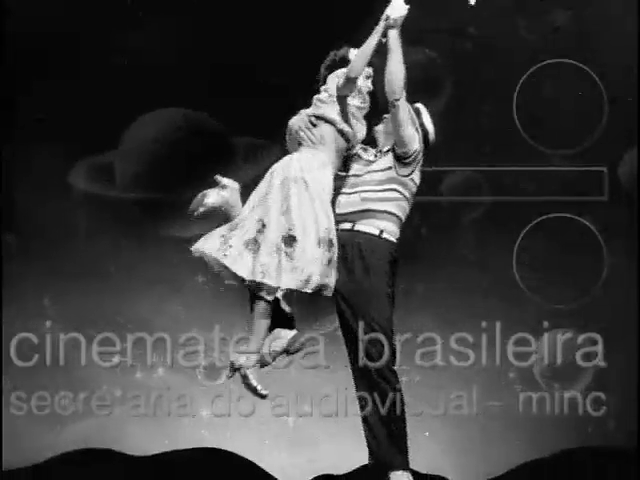
\includegraphics[width=0.7\textwidth]{chapters/cap-historia-passos/elevador1950.png}
  \caption{Fotograma do tempo 1 do passo elevador, tirado do filme ``Aviso aos navegantes'' (1950) \cite[min. 40:35]{AtlantidaDance}.}
  \label{fig:elevador50}
\end{figure}
\end{comment}



%%%%%%%%%%%%%%%%%%%%%%%%%%%%%%%%%%%%%%%%%%%%%%%%%%%%%%%%%%%%%%%%%%%%%%%%%%%%%%%
\subsection{Cruzado}
\index{Passo!Cruzado}
\index{Passo cíclico!Cruzado}
\index{Passo simétrico!Cruzado}
%%                CICLICO     |SIMETRICO   |CONTRATEMPO   |DESLOCAMENTOS |TIEMPOS
\caracterpasso{\CheckedItem}{\CheckedItem}{\NoCheckedItem}{\NoCheckedItem}{4}
Este movimento de samba de gafieira não tem uma data de criação conhecida \cite[pp. 143]{perna2002samba};
porem, podemos ver uma menção a este movimento, junto a outros conhecidos neste estilo,
em 1976 na revista ``Veja'' \cite[pp. 158]{1976veja},
em 1978 na letra da canção ``Baile no Elite'' \cite{BaileNoElite}  e 
em 1979 na revista ``Isto é'' \cite[pp. 89]{revista1979isto},
pelo que podemos estabelecer sua data de criação em algum momento anterior a 1976.

No \AnoLivro, este é um \hyperref[def:PassoCiclico]{\textbf{passo cíclico}} que dura 4 tempos;
e inicia na postura de X com um \hyperref[def:abracodedanca]{\textbf{abraço de dança}}.
Em todo o movimento este abraço se mantêm e os dois primeiros tempos 
são simétricos aos dois últimos, porem com os pés trocados (direita por esquerda). 
Assim, para atingir o tempo 1, se muda a uma postura frente a frente desde a postura de X;
para conseguir isto o \hyperref[def:Condutor]{\textbf{condutor}} 
leva sua perna esquerda para a frente e o \hyperref[def:Seguidor]{\textbf{seguidor}}  a direita para atrás,
em ambos casos, os movimentos estão em referencia a seus 
respetivos \hyperref[def:PlanoFrontal]{\textbf{planos frontais}} e 
se pisa e se transfere o peso do corpo no tempo 1.
No tempo 1.5 ambos dançarinos realizam só uma transferência de peso (sem deslocamento),
o condutor para sua perna direita e o seguidor para sua esquerda.
No tempo 2 ambos dançarinos cruzam as pernas, 
o condutor cruza a perna esquerda por frente da direita, e o seguidor a perna direita por trás da esquerda.
Neste ponto o par se encontra numa postura similar a postura de X, 
com diferencia que na postura de X é a perna esquerda de ambos que fica uma próxima a outra,
e nesta última postura são as pernas esquerdas que ficam próximas.
Nos tempos 3, 3.5 e 4, se repete a essência do movimento anteriormente descrito;
é dizer, se abre a uma postura frente a frente, se ajeita o peso do corpo e finalmente se cruzam as pernas;
chegando no tempo 4 na postura de X.


%%%%%%%%%%%%%%%%%%%%%%%%%%%%%%%%%%%%%%%%%%%%%%%%%%%%%%%%%%%%%%%%%%%%%%%%%%%%%%%
\subsection{Cadeirinha}
%\index{Passo!Cadeirinha}
\index{Postura!Cadeirinha}
\index{Postura de finalização!Cadeirinha}


Uma postura com as caraterísticas do que no \AnoLivro~ conhecemos como cadeirinha, 
pode ser visto no filme ``Aviso aos navegantes'' (1950),
pelo que podemos especular que este existia desde muito antes \cite[min. 40:35]{AtlantidaDance}.
\begin{comment}
A Figura \ref{fig:cadeirinha1950} mostra um fotograma deste filme, onde se observa a cadeirinha.
\begin{figure}[h!]
  \centering
    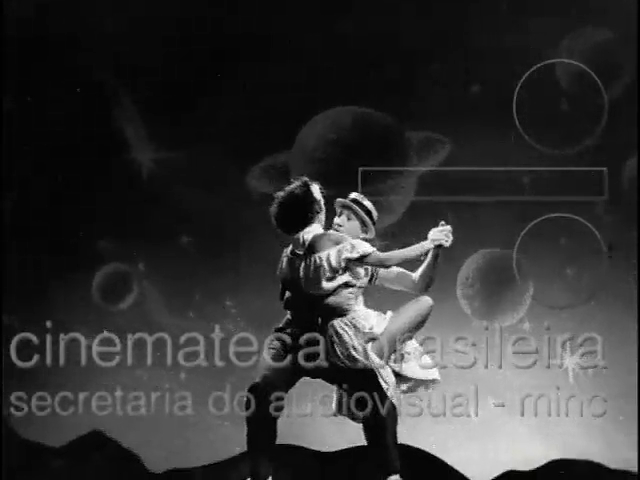
\includegraphics[width=0.7\textwidth]{chapters/cap-historia-passos/cadeirinha1950.png}
  \caption{Fotograma da cadeirinha, tirado do filme ``Aviso aos navegantes'' (1950) \cite[min. 40:35]{AtlantidaDance}.}
  \label{fig:cadeirinha1950}
\end{figure}
\end{comment}
Posteriormente, é possível achar o passo numa fotografia com a postura final caraterística da cadeirinha, 
no ``jornal dos sports''(RJ),
do dia 17 de julho de 1986 \cite[pp. 6]{gafieiraaredeout2}. 
\begin{comment}
como pode ser visto na Figura \ref{fig:cadeirinha86}.
\begin{figure}[h!]
  \centering
    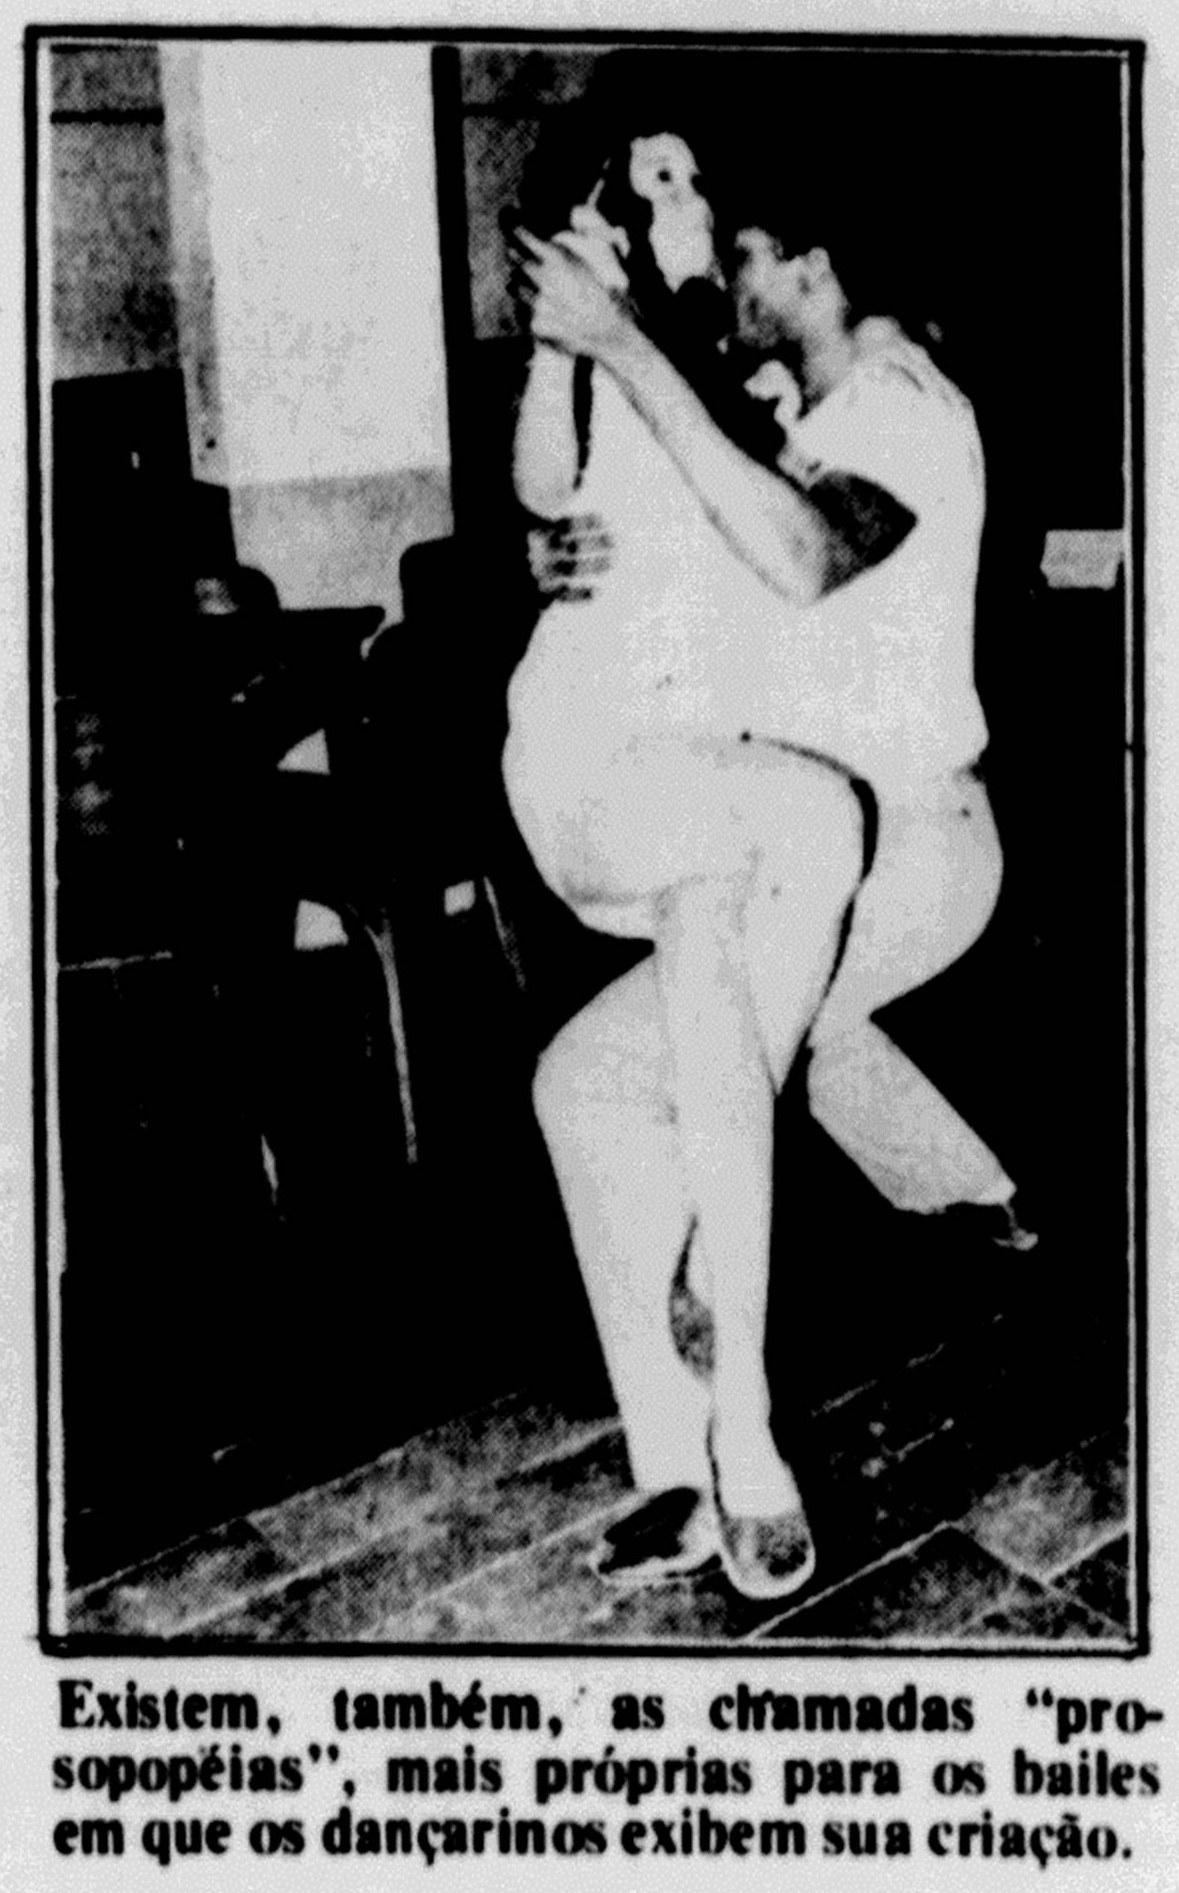
\includegraphics[width=0.45\textwidth]{chapters/cap-historia-passos/cadeirnha1986.jpg}
  \caption{Fotografia da postura da cadeirinha, publicada em 1986 no ``jornal dos sports''(RJ) \cite[pp. 6]{gafieiraaredeout2}.}
  \label{fig:cadeirinha86}
\end{figure}
\end{comment}

%%                FINALIZA     |TRANSIÇÂO
\caracterpostura{\CheckedItem}{\NoCheckedItem}
No \AnoLivro, o nome cadeirinha representa de forma particular a uma postura onde o \hyperref[def:Seguidor]{\textbf{seguidor}} 
senta-se sobre a perna do \hyperref[def:Condutor]{\textbf{condutor}}  (comumente sobre a perna esquerda);
por outro lado, de forma mais geral  o nome representa a qualquer movimento que tenha como postura final a cadeirinha.
A saída do chão do seguidor pode-se originar desde vários movimentos ou passos,
como por exemplo do  \hyperref[def:PassoBalao]{\textbf{balão}}; porem,
todos conservam a mesma técnica, que ao igual que  no caso do passo  \hyperref[def:PassoElevador]{\textbf{elevador}},
a suspensão no ar do seguidor, é mantida e sustentada pelo braço esquerdo do condutor,
que para este propósito  desce da linha dos ombros.
É importante lembrar que este braço não faz força para levantar ao seguidor, 
e sim simplesmente tenta manter a postura,
o que misturado com o movimento do corpo do condutor (esticar as pernas anteriormente flexionadas, principalmente)
provoca a saída do chão e suspensão do seguidor.

%%%%%%%%%%%%%%%%%%%%%%%%%%%%%%%%%%%%%%%%%%%%%%%%%%%%%%%%%%%%%%%%%%%%%%%%%%%%%%%
\subsection{Bicicleta}
\index{Passo!Bicicleta}

%%                CICLICO     |SIMETRICO      |CONTRATEMPO   |DESLOCAMENTOS |TIEMPOS
\caracterpasso{\NoCheckedItem}{\NoCheckedItem}{\NoCheckedItem}{\NoCheckedItem}{2}
Movimento sem data de criação conhecida \cite[pp. 143,144]{perna2002samba}.
Porem, podemos ver uma menção a este movimento, junto a outros conhecidos no samba de gafieira, 
em 1979 na revista ``Isto é'' \cite[pp. 89]{revista1979isto}.

No \AnoLivro, o nome bicicleta representa a um movimento da família das escovinhas,
especialmente emparentado com o tipo de escovinhas que chutam para atrás.
Uma vez entrado no movimento da bicicleta é possível pedalar (ou escovar) indefinidamente;
porem isto é pouco comum, na pratica é comum ver só 3 chutes (em 2 tempos) ou 5 chutes (em 3 tempos) ,
pelo que no movimento, mesmo tendo a possibilidade, 
não se executam as pedaladas ou escovadas da contraparte simétrica do primeiro grupo de 3 chutes,
que levariam a completar um ciclo;
pois isto obrigaria a alongar a duração do movimento a mais de 3 tempos,
o que jogaria em contra do espirito deste que é a surpresa.

Existem varias formas para chegar a postura inicial da bicicleta,  
a forma mais simples é a partir do \hyperref[def:abracodedanca]{\textbf{abraço de dança}},
estando o par, frente a frente, 
e com o peso do corpo no lado do pé esquerdo do \hyperref[def:Condutor]{\textbf{condutor}}.
Nesse momento, se o condutor é quem realizará a bicicleta, 
este leva o pé direito atrás,
deixando numa postura estática ao \hyperref[def:Seguidor]{\textbf{seguidor}} 
que servirá de apoio ou referencia;   
o condutor estará ligeiramente inclinado,
procurando ficar numa postura perpendicular entre os planos frontais de ambos dançarinos.
É nesse ponto que o condutor, escova 3 vesses para atrás iniciando com o pé direito,
no tempos 1, 1.5 e 2. No casos que sejam 5 escovadas, se chuta nos tempos,
1, 1.5, 2, 2.5 e 3. No final o condutor termina com o peso do corpo na perna direita,
e pode sair dessa postura, uma forma interessante é fazendo ambos uma tesoura.

%%%%%%%%%%%%%%%%%%%%%%%%%%%%%%%%%%%%%%%%%%%%%%%%%%%%%%%%%%%%%%%%%%%%%%%%%%%%%%%
%%%%%%%%%%%%%%%%%%%%%%%%%%%%%%%%%%%%%%%%%%%%%%%%%%%%%%%%%%%%%%%%%%%%%%%%%%%%%%%
\PRLsep{Passos no samba de gafieira anteriores a 1990}

%%%%%%%%%%%%%%%%%%%%%%%%%%%%%%%%%%%%%%%%%%%%%%%%%%%%%%%%%%%%%%%%%%%%%%%%%%%%%%%
\subsection{ Picadinho (Picadilho)}
\index{Passo!Picadilho}
\index{Passo!Picadinho}
\index{Passo cíclico!Picadinho}
\index{Passo simétrico!Picadinho}
\index{Passo de deslocamento!Picadinho}


Em palavras de Jimmy de Oliveira este movimento já existia antes de 1990 \cite{sambafunkeadoJimmyDeOliveiraPart1}.
Na década de 1920, podemos ver na revista ``A Cigarra'', 
referencias a um tipo de música e de dança denominado picadinho,
geralmente indicado com frases como \cite[pp. 13]{picadinho1}:
\begin{citando}
O chefe da turma é Zezé de Almeida, excellente pianista,
que nos entontece, quando toca os seus \textbf{picadinhos} apimentados;~\\
$[$...$]$~\\
é o Deco. Que rapasinho admiravel.. para dansar \textbf{picadinho}! 
Zezé tocando e Deco dansando, tenho eu divertimento 
para toda a vida e mais seis mezes.
\end{citando}
Em números posteriores da revista, 
podemos achar outras referencias ao picadinho como dança \cite[pp. 52]{picadinho2} \cite[pp. 49]{picadinho3}.

%%                CICLICO     |SIMETRICO   |CONTRATEMPO   |DESLOCAMENTOS |TIEMPOS
\caracterpasso{\CheckedItem}{\CheckedItem}{\NoCheckedItem}{\CheckedItem}{4}
O picadilho ou picadinho, no \AnoLivro~ é um movimento de pouco deslocamento, 
se realiza com um abraço mais folgado, 
para dar espaço ao movimento do \hyperref[def:Seguidor]{\textbf{seguidor}}.
Cada ciclo do movimente dura 4 tempos, sendo o primeiro par de tempos do passo, simétrico ao segundo.


Para uma correta execução do movimento, 
o \hyperref[def:Condutor]{\textbf{condutor}} envia informação de condução mediante o \hyperref[def:abracodedanca]{\textbf{abraço de dança}},
de modo que esta informação chegue quase sem degradação ate o quadril do seguidor,
é nesse ponto que a condução provoca o movimento das pernas (uma por vez), de modo que
o seguidor mantêm em todo momento as ``pernas fechadas''\footnote{
Ter as pernas fechadas, neste contexto, não indica literalmente ter as pernas juntas, 
e sim juntar as pernas como se em todo momento ao caminhar tentássemos segurar uma folha de papel na virilha.}.
Assim, na primeira metade do ciclo do passo, no tempo 1, o seguidor,
da inicialmente um passo ao frente ganhando o peso do corpo, 
logo no tempo 1.5 o pé livre que está atrás faz um movimento para fechar mais as pernas, 
ganhando este pé o peso do corpo; finalmente, o novo pé livre se movimenta ligeiramente ao frente no tempo 2, 
para ajeitar a postura e ganhar o peso do corpo, neste caso se descansa um tempo 2 completo.
A segunda metade do ciclo é similar à primeira e inicia no tempo 3, só que agora se começa com o outro pé, 
o pé livre do peso do corpo.


%%%%%%%%%%%%%%%%%%%%%%%%%%%%%%%%%%%%%%%%%%%%%%%%%%%%%%%%%%%%%%%%%%%%%%%%%%%%%%%
%%%%%%%%%%%%%%%%%%%%%%%%%%%%%%%%%%%%%%%%%%%%%%%%%%%%%%%%%%%%%%%%%%%%%%%%%%%%%%%
\PRLsep{Passos de samba de gafieira nas décadas 1980 e 1990}

%%%%%%%%%%%%%%%%%%%%%%%%%%%%%%%%%%%%%%%%%%%%%%%%%%%%%%%%%%%%%%%%%%%%%%%%%%%%%%%
\subsection{\textcolor{blue}{Caminhada}} 
\index{Passo!Caminhada a contratempo}
\index{Passo cíclico!Caminhada a contratempo}
\index{Passo a contratempo!Caminhada a contratempo}
 Caminhada ou caminhada a contratempo.
Este passo foi  criado entre o final da década de 1980 e inícios de 1990  \cite[pp. 143]{perna2002samba}.

%%%%%%%%%%%%%%%%%%%%%%%%%%%%%%%%%%%%%%%%%%%%%%%%%%%%%%%%%%%%%%%%%%%%%%%%%%%%%%%
\subsection{\textcolor{blue}{Chicote}} 
\index{Passo!Chicote}
Este passo foi  criado entre o final da década de 1980 e inícios de 1990  \cite[pp. 143]{perna2002samba}.

%%%%%%%%%%%%%%%%%%%%%%%%%%%%%%%%%%%%%%%%%%%%%%%%%%%%%%%%%%%%%%%%%%%%%%%%%%%%%%%
\subsection{\textcolor{blue}{Giro da dama}}
\index{Passo!Giro da dama}
Movimento criado por Jaime Arôxa, entre os anos de 1987 a 1990 \cite{EntrevistaJaimeAroxa1} \cite[pp. 144]{perna2002samba}.


%%%%%%%%%%%%%%%%%%%%%%%%%%%%%%%%%%%%%%%%%%%%%%%%%%%%%%%%%%%%%%%%%%%%%%%%%%%%%%%
\subsection{\textcolor{blue}{Tirada de perna}}
\index{Passo!Tirada de perna}
Movimento criado por Jaime Arôxa, entre os anos de 1987 a 1990,
este movimento teve influencias das aulas de tango ditadas por Jaime \cite{EntrevistaJaimeAroxa1} \cite[pp. 144]{perna2002samba}.

%%%%%%%%%%%%%%%%%%%%%%%%%%%%%%%%%%%%%%%%%%%%%%%%%%%%%%%%%%%%%%%%%%%%%%%%%%%%%%%
\subsection{\textcolor{blue}{Esse}}
\index{Passo cíclico!Esse} 
\index{Passo!Esse}
Este passo foi  criado entre o final da década de 1980 e inícios de 1990  \cite[pp. 143]{perna2002samba}.

%%%%%%%%%%%%%%%%%%%%%%%%%%%%%%%%%%%%%%%%%%%%%%%%%%%%%%%%%%%%%%%%%%%%%%%%%%%%%%%
\subsection{Facão}
\label{subsec:desc:passo:facao}
\index{Passo!Facão}
\index{Postura de finalização!Facão}

%%                FINALIZA     |TRANSIÇÂO
\caracterpostura{\CheckedItem}{\NoCheckedItem}
Esta postura ou passo foi  criado entre o final da década de 1980 e inícios de 1990  \cite[pp. 143]{perna2002samba}.
Porem na década de 1950 existia um movimento que tinha um final semelhante a esta postura, 
este se chamava ``joelhada'' \cite[pp. 160]{fornaciari1950aprender};
porem, o abraço  não era colado,
e sim mais aberto de modo que o casal terminava tendo contato só nos joelhos.
Assim, a joelhada pode ter sido o precursor ou quem inspirou a criação do facão.

Voltando ao facão de \AnoLivro, pessoalmente entendo mais este como uma postura que 
como um movimento ou passo. Isto é porque existem varias formas pra chegar à postura do facão,
de modo que é difícil apontar uma delas para assumir o nome de facão sobre as outras.

A postura do facão, é uma onde o par de dança está num abraçado colado e frente a frente, 
de modo que ambos tem a perna direita um pouco atrás do \hyperref[def:PlanoFrontal]{\textbf{plano frontal}} da linha da cabeça,
e a perna esquerda um pouco adiante no mesmo plano; com esta descrição se deduz 
que ambos tem o peso do corpo dividido em ambos pés; pelo que esta postura,
deve entende-se como uma de descanso, momentâneo porem descanso;
é dizer, se nossa dança fosse um relato escrito, a postura do facão
representaria um ponto, ou em alguns casos um ponto e virgula.
Se o que pretendemos representar é um ponto e virgula, 
é interessante não dividir o peso do corpo 50\% e 50\% em ambos pés,
e sim carregar o peso do corpo um pouco mais em um 
para poder liberar facilmente u outro pé para poder sair da postura de facão elegantemente.  

Sobre as formas de chegar a postura do facão, a continuação será descrita a forma mais simples,
porem não a mais interessante. Iniciamos desde o passo, frente-trás também chamado básico, 
ou básico linear no samba de gafieira. Desde o ponto de vista do \hyperref[def:Condutor]{\textbf{condutor}}, 
com um \hyperref[def:abracodedanca]{\textbf{abraço de dança}} colado,
damos primeiro duas pisadas no lugar, iniciando com a perna esquerda no tempo 1, e logo a perna direita no tempo 1.5,
logo damos um passo atrás com a perna direita no tempo 2; 
finalmente no tempo 3 damos mais um passo atrás com a perna direita, 
e se temos mantido o abraço colado, 
o \hyperref[def:Seguidor]{\textbf{seguidor}} sentirá a necessidade de dar um passo a frente com a perna esquerda,
chegando ambos à postura do facão.  

Este movimento linear para atrás e pouco interessante para chegar ao facão, mas pode ser apimentado,
se usamos um movimento sinuoso para atrás (em vez de um linear), este movimento,
é promovido pelo condutor, e tem forma de ``S'' onde a ligeira curva para a esquerda é realizada no tempo 1 e 1.5,
no tempo  2 chegamos ao ponto neutro o meio, onde a curva esta sobre a linha reta, e para chegar a 3, 
que também está sobre a linha reta e ao final de ambas curvas,
o condutor promove a curva para a sua direita.

%%%%%%%%%%%%%%%%%%%%%%%%%%%%%%%%%%%%%%%%%%%%%%%%%%%%%%%%%%%%%%%%%%%%%%%%%%%%%%%
\subsection{Faquinha}
\index{Passo!Faquinha}
%%                CICLICO     |SIMETRICO   |CONTRATEMPO   |DESLOCAMENTOS |TIEMPOS
\caracterpasso{\CheckedItem}{\NoCheckedItem}{\NoCheckedItem}{\CheckedItem}{2}
Este passo foi  criado entre o final da década de 1980 e inícios de 1990  \cite[pp. 143]{perna2002samba}.
É uma variante do  \hyperref[subsec:desc:passo:facao]{\textbf{facão}} (passo), 
com a diferencia que o movimento tem uma postura final (facão) menos acentuada;
sendo mais parecido a um casal num \hyperref[def:abracodedanca]{\textbf{abraço de dança}} colado, 
na postura frente a frente  e com uma perna ligeiramente adiantada a outra;
com diferencia da postura de facão, 
onde as pernas tem uma separação que claramente evidencia uma postura do descanso;
a faquinha, pelo contrario, termina numa postura final de transição, 
pois comumente são realizadas varias faquinhas de forma consecutiva antes de realizar um facão,
 para assim finalizar a sequencia de forma mais acentuada.

O passo faquinha dura dois tempos, e consta de dois movimentos, 
onde a postura final é igual à inicial de modo que o passo pode repetir-se ciclicamente indefinidamente.
O movimento inicia quando o par de dança está numa postura de facão pouco acentuada;
é dizer, quando cada um tem pouca separação entre os pés; 
e o peso do corpo está do lado da perna direita do \hyperref[def:Condutor]{\textbf{condutor}}.
Logo, no primeiro tempo, 
o condutor junta os pés trazendo sua pé esquerdo junto à direito e trocando o peso do corpo a esse pé,
mantendo o abraço para provocar um movimento simétrico no \hyperref[def:Seguidor]{\textbf{seguidor}};
porem a ação do movimento dos pés não é uma causa e sim um efeito,
pois é provocado por uma condução do tórax usando que é transmitida por médio do abraço colado;
para isto o condutor gira o tórax no sentido horário no \hyperref[def:PlanoAxial]{\textbf{plano axial}},
tentando suspender ligeiramente o corpo do seguidor e o seu próprio.
No segundo tempo, o condutor dá um passo atrás com sua perna direita,
 mantendo o abraço colado e provocando que o seguidor de um passo adiante com sua perna esquerda,
chegando novamente a posição inicial.



%%%%%%%%%%%%%%%%%%%%%%%%%%%%%%%%%%%%%%%%%%%%%%%%%%%%%%%%%%%%%%%%%%%%%%%%%%%%%%%
\subsection{\textcolor{blue}{Gancho}} 
\index{Passo!Gancho}
Este passo foi  criado entre o final da década de 1980 e inícios de 1990  \cite[pp. 143]{perna2002samba}.

%%%%%%%%%%%%%%%%%%%%%%%%%%%%%%%%%%%%%%%%%%%%%%%%%%%%%%%%%%%%%%%%%%%%%%%%%%%%%%%
\subsection{\textcolor{blue}{Gancho redondo}} 
\index{Passo!Gancho redondo}
Este passo foi  criado entre o final da década de 1980 e inícios de 1990  \cite[pp. 143]{perna2002samba}.

%%%%%%%%%%%%%%%%%%%%%%%%%%%%%%%%%%%%%%%%%%%%%%%%%%%%%%%%%%%%%%%%%%%%%%%%%%%%%%%
\subsection{\textcolor{blue}{Letra}}
\index{Passo!Letra}
Este passo foi  criado entre o final da década de 1980 e inícios de 1990  \cite[pp. 143]{perna2002samba}.

%%%%%%%%%%%%%%%%%%%%%%%%%%%%%%%%%%%%%%%%%%%%%%%%%%%%%%%%%%%%%%%%%%%%%%%%%%%%%%%
\subsection{\textcolor{blue}{Puladinho redondo}} 
\index{Passo!Puladinho redondo}
Este passo foi  criado entre o final da década de 1980 e inícios de 1990  \cite[pp. 143]{perna2002samba}.

%%%%%%%%%%%%%%%%%%%%%%%%%%%%%%%%%%%%%%%%%%%%%%%%%%%%%%%%%%%%%%%%%%%%%%%%%%%%%%%
\subsection{\textcolor{blue}{Trança}}
\index{Passo cíclico!Trança}
\index{Passo!Trança}
Este movimento é antigo, porem Jaime Arôxa trabalhou sobre ele entre os anos de 1987 a 1990,
pois não existia uma didática para o ensino do movimento, 
e era realizado apenas pelos homens; 
de modo que Jaime agregou a parte do seguidor no par de dança  \cite{EntrevistaJaimeAroxa1} \cite[pp. 143]{perna2002samba}.
%%%%%%%%%%%%%%%%%%%%%%%%%%%%%%%%%%%%%%%%%%%%%%%%%%%%%%%%%%%%%%%%%%%%%%%%%%%%%%%
\subsection{\textcolor{blue}{Tesoura}}
\index{Passo!Tesoura}
Movimento criado por Jaime Arôxa, entre os anos de 1987 a 1990 \cite{EntrevistaJaimeAroxa1} \cite[pp. 143]{perna2002samba}.

%%%%%%%%%%%%%%%%%%%%%%%%%%%%%%%%%%%%%%%%%%%%%%%%%%%%%%%%%%%%%%%%%%%%%%%%%%%%%%%
%%%%%%%%%%%%%%%%%%%%%%%%%%%%%%%%%%%%%%%%%%%%%%%%%%%%%%%%%%%%%%%%%%%%%%%%%%%%%%%
\PRLsep{Passos de samba de gafieira da décadas de 1990}

%%%%%%%%%%%%%%%%%%%%%%%%%%%%%%%%%%%%%%%%%%%%%%%%%%%%%%%%%%%%%%%%%%%%%%%%%%%%%%%
\subsection{\textcolor{blue}{Assalto}} 
\index{Passo!Assalto}
\index{Passo cíclico!Assalto}
Este passo foi criado por Jimmy de Oliveira apos o ano 1990 \cite{sambafunkeadoJimmyDeOliveiraPart1}.

%%%%%%%%%%%%%%%%%%%%%%%%%%%%%%%%%%%%%%%%%%%%%%%%%%%%%%%%%%%%%%%%%%%%%%%%%%%%%%%
\subsection{\textcolor{blue}{Boneca}} 
\index{Passo!Boneca}
Este passo foi criado por Jimmy de Oliveira apos o ano 1990 \cite{sambafunkeadoJimmyDeOliveiraPart1}.

%%%%%%%%%%%%%%%%%%%%%%%%%%%%%%%%%%%%%%%%%%%%%%%%%%%%%%%%%%%%%%%%%%%%%%%%%%%%%%%
\subsection{\textcolor{blue}{Elástico}} 
\index{Passo!Elastico}
Este passo foi criado por Jimmy de Oliveira apos o ano 1990 \cite{sambafunkeadoJimmyDeOliveiraPart1}.

%%%%%%%%%%%%%%%%%%%%%%%%%%%%%%%%%%%%%%%%%%%%%%%%%%%%%%%%%%%%%%%%%%%%%%%%%%%%%%%
\subsection{\textcolor{blue}{Escovinha}}
\index{Passo cíclico!Escovinha}
\index{Passo!Escovinha}
Este passo foi criado por Jimmy de Oliveira apos o ano 1990 \cite{sambafunkeadoJimmyDeOliveiraPart1}.

%%%%%%%%%%%%%%%%%%%%%%%%%%%%%%%%%%%%%%%%%%%%%%%%%%%%%%%%%%%%%%%%%%%%%%%%%%%%%%%
%\subsection{Homem na lua}
%Este passo foi criado por Jimmy de Oliveira apos o ano 1990 \cite{sambafunkeadoJimmyDeOliveiraPart1}.

%%%%%%%%%%%%%%%%%%%%%%%%%%%%%%%%%%%%%%%%%%%%%%%%%%%%%%%%%%%%%%%%%%%%%%%%%%%%%%%
\subsection{\textcolor{blue}{Pescaria}} 
\index{Passo!Pescaria}
Este passo foi criado por Jimmy de Oliveira apos o ano 1990 \cite{sambafunkeadoJimmyDeOliveiraPart1}.

%%%%%%%%%%%%%%%%%%%%%%%%%%%%%%%%%%%%%%%%%%%%%%%%%%%%%%%%%%%%%%%%%%%%%%%%%%%%%%%
\subsection{\textcolor{blue}{Romário}}
\label{subsec:passo:romario}
\index{Passo cíclico!Romário} 
\index{Passo!Romário}
Este passo foi criado por Jimmy de Oliveira apos o ano 1990 \cite{sambafunkeadoJimmyDeOliveiraPart1}.


%%%%%%%%%%%%%%%%%%%%%%%%%%%%%%%%%%%%%%%%%%%%%%%%%%%%%%%%%%%%%%%%%%%%%%%%%%%%%%%
%%%%%%%%%%%%%%%%%%%%%%%%%%%%%%%%%%%%%%%%%%%%%%%%%%%%%%%%%%%%%%%%%%%%%%%%%%%%%%%
\PRLsep{Passos de samba de gafieira sem data conhecida}



%%%%%%%%%%%%%%%%%%%%%%%%%%%%%%%%%%%%%%%%%%%%%%%%%%%%%%%%%%%%%%%%%%%%%%%%%%%%%%%
\subsection{\textcolor{blue}{Balanço}}
\index{Passo!Balanço}
\index{Passo cíclico!Balanço}
Movimento sem data de criação conhecida, 
seguindo Jaime Arôxa o balanço sempre existiu desde do início do século, 
no maxixe \cite{EntrevistaJaimeAroxa1} \cite[pp. 144]{perna2002samba}.


%%%%%%%%%%%%%%%%%%%%%%%%%%%%%%%%%%%%%%%%%%%%%%%%%%%%%%%%%%%%%%%%%%%%%%%%%%%%%%%
\subsection{\textcolor{blue}{Saída lateral}}
\index{Passo!Saída lateral}
Movimento sem data de criação conhecida \cite[pp. 144]{perna2002samba}.

%%%%%%%%%%%%%%%%%%%%%%%%%%%%%%%%%%%%%%%%%%%%%%%%%%%%%%%%%%%%%%%%%%%%%%%%%%%%%%%
\subsection{\textcolor{blue}{Tirada ao lado}}
\index{Passo!Tirada ao lado}
Movimento sem data de criação conhecida \cite[pp. 144]{perna2002samba}.

%%%%%%%%%%%%%%%%%%%%%%%%%%%%%%%%%%%%%%%%%%%%%%%%%%%%%%%%%%%%%%%%%%%%%%%%%%%%%%%
\subsection{\textcolor{blue}{Mestre sala}}
\index{Passo!Mestre sala}
Movimento sem data de criação conhecida \cite[pp. 144]{perna2002samba}.



%%%%%%%%%%%%%%%%%%%%%%%%%%%%%%%%%%%%%%%%%%%%%%%%%%%%%%%%%%%%%%%%%%%%%%%%%%%%%%%
\subsection{\textcolor{blue}{Enceradeira}}
\index{Passo!Enceradeira}
Movimento sem data de criação conhecida \cite[pp. 144]{perna2002samba}.


\begin{comment}

Passos acrobáticos ou para apresentações \cite[pp. 142-143]{perna2002samba}:
\begin{tasks}
\task \textbf{Cabide}, \index{Passo!Cabide} oriundo do rock.
\task \textbf{Baratinha} \index{Passo!Baratinha}
\task \textbf{Enceradeira}, \index{Passo!Enceradeira} criado em algum momento no final da década de 1980 e inícios da década de 1990.
\end{tasks}
\end{comment}

%%%%%%%%%%%%%%%%%%%%%%%%%%%%%%%%%%%%%%%%%%%%%%%%%%%%%%%%%%%%%%%%%%%%%%%%%%%%%%%
%%%%%%%%%%%%%%%%%%%%%%%%%%%%%%%%%%%%%%%%%%%%%%%%%%%%%%%%%%%%%%%%%%%%%%%%%%%%%%%
%%%%%%%%%%%%%%%%%%%%%%%%%%%%%%%%%%%%%%%%%%%%%%%%%%%%%%%%%%%%%%%%%%%%%%%%%%%%%%%
\section{Sobre o $syllabus$ do samba de gafieira}

O $syllabus$  do samba de gafieira, foi criado no ano 2001 em Rio de Janeiro,
este é um listado de passos ordenado em três níveis (básico, intermediário e avançado),
selecionados por votação,
onde são agrupados passos que se consideram essenciais para o ensino e competição;
neste listado não entram passos aéreos \cite[pp. 144]{perna2002samba}.


As personas que participaram da votação para a elaboração do $syllabus$ são \cite[pp. 144]{perna2002samba}:
\begin{inparaitem}[$*$]
\item Bob Cunha e Aurya
\item Bolacha
\item Bruno Barros
\item Carlinhos de Jesus
\item Dani Aguiar
\item Dani Escudero
\item Dani Galper
\item Egídio
\item Flávio Miguel
\item Gérson Reis
\item Kilve
\item Luis Florião/Adriana
\item Marcello Moragas
\item Marco Antonio Perna
\item Marquinhos Copacabana
\item Rogério Mendonça
\item Valdeci
\item Wanir Almeida
\end{inparaitem}.\\



Os passos de \textbf{nível básico} são:
\begin{tasks}(2)
\task Básico (frente-trás)
\task Balanço 
\task Caminhada (ou caminhada a contratempo)
\task Cruzado
\task Esse
\task Gancho
\task Giro da dama
\task Puladinho
\task Saída lateral
\task Tirada ao lado
\end{tasks}~\\


Os passos de \textbf{nível intermediário} são:
\begin{tasks}(2)
\task Assalto
\task Balão apagado
\task Escovinha
\task Facão
\task Gancho redondo
\task Mestre sala
\task Romário
\task Tesoura
\task Tirada de perna
\task Trança
\end{tasks}~\\

Os passos de \textbf{nível avançado} são:
\begin{tasks}(2)
\task Bicicleta
\task Enceradeira
\task Pião
\task Picadinho (ou ou picadilho)
\task Pica-pau
\end{tasks}



%----------------------------------------------------------------------------------------
%----------------------------------------------------------------------------------------
%----------------------------------------------------------------------------------------
%	PART
%----------------------------------------------------------------------------------------
\part{Musicalização para a dança}

\chapterimage{chapter_head_2.pdf} % Chapter heading image

\chapter{Fundamentos de notação musical}
Nas seguintes sub seções abordaremos alguns conceitos de notação musical;
porem, não aprofundaremos demasiado em toda a teoria musical, 
devido a que as explicações mostradas aqui, estão
orientadas para um público interessado na dança, que numa primeira 
aproximação à música, precisa conhecer rapidamente conceitos básicos. 
Mas, empoderamos a curiosidade de todos os leitores a aprofundar mais nestos temas, 
para este efeito existem na literatura muitos materiais, livros ou revistas especializadas 
\cite{medteoria}        %% Teoria Da Musica
\cite{cardoso1973curso} %% Curso Completo De Teoria Musical E Solfejo - 1o Vol.
\cite{mascarenhascurso} %% Curso Completo De Teoria Musical E Solfejo - 2o Vol.
\cite{grabner2001teoria}%% Teoría general de la música 
\cite{alves2004teoria}  %% teoria musical lições essenciais
\cite{apel1969harvard}  %% harvard diccionario
\cite{azevedocompor}    %% Como Compor Música Facilmente: métodos ou estudos para teoria, canto e solfejo (NOPDF)
\cite{adolfo2002musica}.%% Musica: Leitura, Conceitos, Exercicios (NOPDF)

%%%%%%%%%%%%%%%%%%%%%%%%%%%%%%%%%%%%%%%%%%%%%%%%%%%%%%%%%%%%%%%%%%%%%%%%%%%%%%%%

%%%%%%%%%%%%%%%%%%%%%%%%%%%%%%%%%%%%%%%%%%%%%%%%%%%%%%%%%%%%%%%%%%%%%%%%%%%%%%%%
\section{Componentes da música}

A música; na sua forma mais básica,  é um conjunto de sons; esta é criada ao combinar na justa medida: 
ingênio, técnica e arte.

Entre as características de um som temos \cite[pp. 12]{medteoria} :
\begin{description}
\item [Altura:] \label{sec:pos:Altura} 
Também chamado \textbf{tom}\footnote{A palavra tom tem vários significados em música, 
outro significado pode ser um intervalo ou distancia em frequência, 
utilizado na escala diatônica, para mais detalhes ir a Seção \ref{sec:notasmusicais}}, representa a frequência de vibração (principal) da onda mecânica que gera o sonido.
Isto é, que terão um altura maior os sonidos com maior frequência de vibração mecânica (mais agudos), 
e uma altura menor sonidos mais graves.
\begin{example}
A campainha pra chamar ao atendente de um hotel tem uma altura maior,
que a campana da igreja, que é tocada ao médio dia, que tem um sonido mais grave.
\end{example} 
\index{Altura}\index{Tom}
\item [Duração:] \label{sec:pos:Duracion}
Representa a longitude temporal, durante o qual um sonido será executado.
\begin{example}
Podemos assoviar durante um tempo, curto, longo, muito longo, etc.
\end{example} 
\index{Duração}
\item [Intensidade:] \label{sec:pos:Intensidade}
Se refere ao volume sonoro ou à potencia do sonido executado, 
de modo que o som pode ter intensidades, por exemplo: fracas, fortes, muito fortes, etc.  
\begin{example}
Si escolhemos dois pedaços de madeira e batimos eles um contra outro, 
podemos gerar sons com diferente intensidade, dependendo da força com que realizemos os batimentos.
\end{example} 
\index{Intensidade}
\item [Timbre:] \label{sec:pos:timbre}
Na definição da altura de um som, referenciamos esta seguindo a sua frequência principal,
porem um som não está composto exclusivamente por vibrações a esta frequência.
Na pratica os sons contem muitas outras frequências de vibração, acontecendo simultaneamente e 
que se manifestam com menor intensidade.
A combinação de todas estas frequências de vibração é o que gera o som que escutamos;
assim, a essa especifica configuração de frequências a chamamos como o timbre ou
a ``\textbf{cor}'' do som.
\begin{example}
Se geramos dois sonidos com a mesma altura; mas, um sonido executado por uma flauta,
e o outro por um violão, ambos sonidos terão diferentes timbres ou cores.
\end{example} 
\index{Timbre}
\end{description}
~\\

Conhecidas estas definições básicas, e procurando estruturas mais complexas na música,
podemos distinguir alguns componentes com que esta é constituída, 
por exemplo temos:

\begin{description}
\item [Ritmo:] \label{sec:pos:Ritmo}
Se refere a distribuição temporal da execução dos sonidos e a proporção na duração destes. 
Asim, o ritmo carateriza a música no âmbito temporal \cite[pp. 11]{medteoria}.
\index{Ritmo}
\begin{example}
Batendo palmas, criamos a sequencia de sonidos: palmas, pausa curta, palmas, palmas, pausa loga e palmas.
\end{example} 
\item [Melodia:] \label{sec:pos:Melodia}
É um conjunto de sons, que podem ter diferentes \hyperref[sec:pos:Altura]{\textbf{alturas}}, 
e que estão dispostos sequencialmente. 
A melodia representa um elemento horizontal\footnote{\label{eixohor}Eixo com múltiplas distribuições de tempo dos sons na música} na musica, 
e esta é indivisível do ritmo \cite[pp. 517]{apel1969harvard} \cite[pp. 11]{medteoria}.
\begin{example}
Se assoviamos ``parabéns pra você'', estamos executando uma melodia 
(executando diferentes sons numa distribuição temporal especifica).
\end{example} 
\index{Melodia} 
\item [Harmonia:] \label{sec:pos:Harmonia}
Conjunto de sons dispostos simultaneamente em \hyperref[sec:pos:Altura]{\textbf{alturas}} diferentes.
A harmonia representa um elemento vertical\footnote{\label{eixover}Eixo com múltiplas distribuições de frequência dos sons na música} na música \cite[pp. 371]{apel1969harvard} \cite[pp. 8]{cardoso1973curso} \cite[pp. 11]{medteoria}. 
\begin{example}
Se num piano pressionamos simultaneamente as teclas: Do, Mi e Sol. Estamos executando uma harmonia.
\end{example} 
\index{Harmonia} 
\item [Contraponto:] \label{sec:pos:Contraponto}
O termo deriva de ``punctus contra punctum'' que significa ``nota contra nota'', 
e por extensão ``melodia contra melodia''. 
Assim, falar de contraponto é equivalente a dizer, dois ou mais melodias executadas simultaneamente  
(concepção horizontal\footref{eixohor} e vertical\footref{eixover} da música)  \cite[pp. 208]{apel1969harvard} \cite[pp. 11]{medteoria}.
\begin{example}
Uma orquestra com vários músicos tocando cada um uma melodia.
\end{example} 
\index{Contraponto}
\end{description}


 %[OK]
%%%%%%%%%%%%%%%%%%%%%%%%%%%%%%%%%%%%%%%%%%%%%%%%%%%%%%%%%%%%%%%%%%%%%%%%%%%%%%%%
\section{Figuras musicais, pausas e durações}
\index{Figuras musicais}
\label{sec:figurasmusicais}
As figuras musicais são um conjunto de sinais (desenhos), criadas pra indicar a relação 
entre as \hyperref[sec:pos:Duracion]{\textbf{durações}} dos sons \cite[pp. 20]{medteoria}.
Assim, podemos ver na coluna dois da Tabela \ref{tab:abc-noteslengthbasic}
 um conjunto de 6 destas figuras musicais; 
a primeira coluna representa a longitude temporal (\hyperref[sec:pos:Duracion]{\textbf{duração}}) de cada uma destas figuras;
porem, todos estas durações são relativas ao valor temporal $S$, em segundos, de uma figura \Ganz.
A terceira coluna da tabela contem os nomes de cada uma destas figuras musicais. 
\begin{table}[h]
\centering
\begin{tabular}{|c||c|c||c|c|}
\hline
Duração & Figura & Nome de figura & Pausa & Nome de pausa\\ \hline
\hline
$S$    & \Ganz   & Semibreve    & \GaPa  & Pausa de Semibreve \\ \hline
$S/2$  & \Halb   & Mínima       & \HaPa  & Pausa de Mínima \\ \hline
$S/4$  & \Vier   & Semínima     & \ViPa  & Pausa de Semínima \\ \hline
$S/8$  & \Acht   & Colcheia     & \AcPa  & Pausa de Colcheia \\ \hline
$S/16$ & \Sech   & Semicolcheia & \SePa  & Pausa de Semicolcheia \\ \hline
$S/32$ & \Zwdr   & Fusa         & \ZwPa  & Pausa de fusa  \\ \hline  
\end{tabular}
\caption{Duração e símbolos de algumas figuras musicais}
\label{tab:abc-noteslengthbasic}
\end{table}


\begin{example}
Se decidimos criar uma sequencia rítmica assoviando um único tom, porem
distribuindo os tempos de duração como: Longo, curto, curto; 
repetindo esta sequencia quatro vesses. 
Poderíamos escrever esta sequencia usando figuras musicais numa representação como a mostrada na Figura \ref{fig:abc-figurasexample1}.
É importante ressaltar que assumimos que  um sonido longo dura no tempo exatamente o dobro que um curto, 
e que decidimos\footnote{É escolhida uma semínima porem pode ter sido escolhida 
qualquer outra figura, dado que o valor $S$ não está definido.}
representar um sonido de longa duração como uma semínima.

Para entender melhor a representação com figuras musicais, 
podemos ir a uma representação alternativa com um gráfico da potencia sonora na execução dos sons,
como é representado na Figura \ref{fig:forma-figurasexample1b}.
É fácil perceber como a potencia do som se mantêm, ate justo antes de iniciar 
o seguinte som, de modo que não existem silêncios na sequencia rítmica.
\end{example} 




\begin{figure}[h]
    \centering
    \begin{subfigure}[b]{0.9\textwidth}
 \begin{abc}[name=abc-figurasexample1]
% abcm2ps figurasexample1.abc  -O figurasexample1.ps
% ps2epsi figurasexample1.ps figurasexample1.eps
%
X: 1 % start of header
K: none stafflines=0 %K: C %% Escala de C mayor %
M:  none % M: 2/4
%T: Contratempo num compasso binário
V:1 clef=none stem=up %name="Ritmo 1"   sname="Ritmo 1"
%
[V:1] | B2 B1 B1 B2 B1 B1 B2 B1 B1 B2  B1 B1   |
%       
\end{abc}
	\caption{Sequencia rítmica usando semínimas e colcheias.}
	\label{fig:abc-figurasexample1}
    \end{subfigure}
    ~%add desired spacing between images, e. g. ~, \quad, \qquad, \hfill etc. 
      %(or a blank line to force the subfigure onto a new line)
    \begin{subfigure}[b]{0.9\textwidth}
        
\includegraphics[width=\textwidth]{chapters/cap-musica-basica/forma-figurasexample1.eps}
        \caption{Sequencia rítmica usando um gráfico indicando a potencia do sonido.}
        \label{fig:forma-figurasexample1b}
    \end{subfigure}
    \caption{Sequencia rítmica.}\label{fig:total-figurasexample1}
\end{figure}


Por outro lado, assim como a duração do tempo de execução de cada som precisa uma grafia,
os silêncios ou pausas, também precisam ser indicados. 
De modo que, para cada figura musical existe uma grafia que indica um silencio da mesma duração temporal,
como pode ser visto na quarta coluna da Tabela \ref{tab:abc-noteslengthbasic}.
O nome de cada uma destas pausas está descrito na quinta coluna da mesma tabela.

\begin{example}
Similarmente ao exemplo anterior, se decidimos criar uma sequencia rítmica assoviando um único tom, porem
intercalando sons e silêncios, criaremos um padrão rítmico como na Figura \ref{fig:total-figurasexample2}.

Podemos entender melhor a representação com figuras musicais, 
usando a representação com um gráfico da potencia sonora na execução dos sons,
como é representado na Figura \ref{fig:forma-figurasexample2}.
Nela percebemos como a potencia do som se mantêm durante a longitude de tempo estipulada pela figura musical, 
ate justo antes de iniciar o silencio, indicado por uma linha reta horizontal.
\end{example} 

\begin{figure}[h]
    \centering
    \begin{subfigure}[b]{0.9\textwidth}
 \begin{abc}[name=abc-figurasexample2]
% abcm2ps figurasexample2.abc  -O figurasexample2.ps
% ps2epsi figurasexample2.ps figurasexample2.eps
%
X: 1 % start of header
K: none stafflines=0 %K: C %% Escala de C mayor %
M:  none % M: 2/4
%T: Contratempo num compasso binário
V:1 clef=none stem=up %name="Ritmo 1"   sname="Ritmo 1"
%
[V:1] | z1 B1 z1 B1 z2 B1 z1 B1 z1 B1 z2 B1  z1 B1   |
%       
\end{abc}
	\caption{Sequencia rítmica usando  colcheias e silencios.}
	\label{fig:abc-figurasexample2}
    \end{subfigure}
    ~%add desired spacing between images, e. g. ~, \quad, \qquad, \hfill etc. 
      %(or a blank line to force the subfigure onto a new line)
    \begin{subfigure}[b]{0.9\textwidth}
        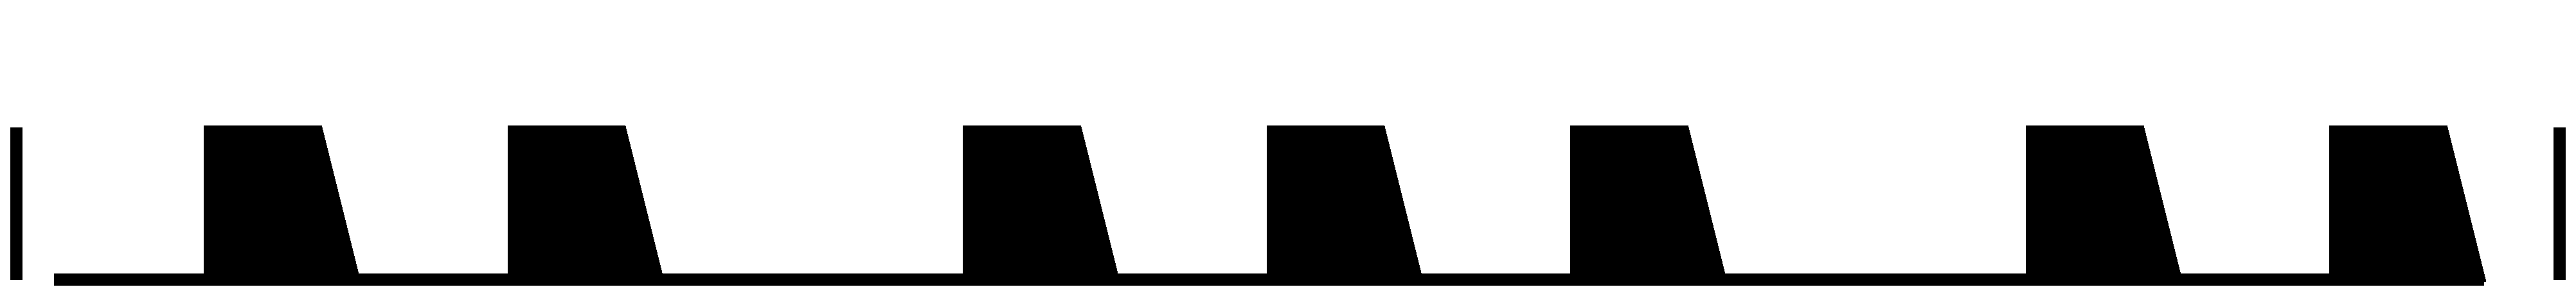
\includegraphics[width=\textwidth]{chapters/cap-musica-basica/forma-figurasexample2.eps}
        \caption{Sequencia rítmica usando um gráfico indicando a potencia do sonido.}
        \label{fig:forma-figurasexample2}
    \end{subfigure}
    \caption{Sequencia rítmica.}\label{fig:total-figurasexample2}
\end{figure}


Ate agora todos os exemplos foram sequencias rítmicas, 
pois não exploramos a possibilidade de variar a altura dos sons;
para poder explorar esta possibilidade devemos ter claro o conceito de pauta,
para que cada figura musical, 
além de nos proporcionar uma informação da \hyperref[sec:pos:Duracion]{\textbf{duração}}  dos sons, 
também nos de informação da \hyperref[sec:pos:Altura]{\textbf{altura}}  destes. 
Tendo estes dois fatores, altura e duração, podemos criar \hyperref[sec:pos:Melodia]{\textbf{melodias}}.

\begin{remark}
O mistério de como distinguir a pausa de mínima (\HaPa) e a pausa de semibreve (\GaPa),
será esclarecido quando desenhemos estes na \hyperref[sec:pauta]{\textbf{pauta}}, ver Seção \ref{sec:tipospauta}.
\end{remark}

\subsection{Ponto de aumento}
\index{Ponto de aumento}
\label{subsec:pontoaumento}
O ponto de aumento é um simbolo que é colocado ao lado direito de uma figura musical ou pausa, 
e este indica um aumento do 50\% na duração \cite[pp. 25]{cardoso1973curso}.
A Tabela \ref{tab:notaspontoadas} mostra esta relação entre as durações.

\begin{table}[h]
\centering
\begin{tabular}{|c||c||c|}
\hline
Duração & Figura & Pausa \\ \hline
\hline
$\frac{3}{2}S$    & \Ganz. =  \Ganz + \Halb   & \GaPa. = \GaPa + \HaPa\\ \hline
$\frac{3}{4}S$    & \Halb. =  \Halb + \Vier   & \HaPa. = \HaPa + \ViPa  \\ \hline
$\frac{3}{8}S$    & \Vier. =  \Vier + \Acht   & \ViPa. = \ViPa + \AcPa  \\ \hline
$\frac{3}{16}S$   & \Acht. =  \Acht + \Sech   & \AcPa. = \AcPa + \SePa  \\ \hline
$\frac{3}{32}S$   & \Sech. =  \Sech + \Zwdr   & \SePa. = \SePa + \ZwPa  \\ \hline
\end{tabular}
\caption{Duração e símbolos de algumas figuras musicais com ponto de aumento}
\label{tab:notaspontoadas}
\end{table}

Da mesma forma que usamos um ponto de aumento, podem ser usados dois ou três pontos de aumento.
\begin{example}
Se usamos dois pontos de aumento a duração de uma nota cresce um 75\%, assim: \Halb.. = \Halb + \Vier + \Acht
\end{example}
\begin{example}
Se usamos tres pontos de aumento a duração de uma nota cresce um 87.5\%, assim: \Vier... = \Vier + \Acht + \Sech + \Zwdr
\end{example}
     %[OK]
%%%%%%%%%%%%%%%%%%%%%%%%%%%%%%%%%%%%%%%%%%%%%%%%%%%%%%%%%%%%%%%%%%%%%%%%%%%%%%%%
\section{Notas musicais}\index{Notas musicais}
\label{sec:notasmusicais}

O sons musicais que representam as notas são sete, 
e foram designadas pelos gregos com as sete primeiras letras do alfabeto,
estes são: \{A, B, C, D, E, F, G\} \cite[pp. 11]{grabner2001teoria} \cite[pp. 9]{cardoso1973curso}.
O ocidente adotou esta forma porem no século XI, 
Guido d'Arezzo rebatizou as notas, 
atribuindo a cada nota a primeira sílaba dos versos
de um hino a São Jõao muito conhecido na época:
\begin{citando}%%
\textbf{Ut} queant laxls,\\
\textbf{re}sonare fibris,\\
\textbf{Mi}ra gestorum,\\
\textbf{fa}muli tuorum,\\
\textbf{Sol}ve polluti,\\
\textbf{La}bii reatum,\\
\textbf{S}ánete lohannes.
\end{citando}
 Assim, apos a troca de ``ut'' por ``do'' nascem as notas musicais: 
\{lá, si, dó, ré, mi, fá, sol\} \cite[pp. 21]{arbones2012armonia} \cite[pp. 7]{cardoso1973curso}. 
A Tabela \ref{tab:notasmusic} mostra a relação entre estas duas notações.

\begin{table}[h]
\centering
\begin{tabular}{|c|c|c|c|c|c|c|}
\hline
A  & B  & C  & D  & E  & F  & G\\ \hline
lá & si & dó & ré & mi & fá & sol \\ \hline
\end{tabular}
\caption{Notas musicais}
\label{tab:notasmusic}
\end{table}

Estas sete notas representam sons com \hyperref[sec:pos:Altura]{\textbf{alturas}} diferentes.
Porem, existem varias formas de atribuir uma \hyperref[sec:pos:Altura]{\textbf{altura}} 
especifica a cada uma destas notas, 
sendo a mais difundida atualmente a afinação (atribuição de alturas) com \hyperref[subsec:tempigual]{\textbf{temperamento igual}}\footnote{O temperamento igual é tratado na Seção \ref{subsec:tempigual}.}.




Conhecida a definição de notas musicais, podemos agora descrever:


\begin{description}
\item [Escala musical:] \label{sec:pos:Escala}
\index{Escala musical}
É uma forma de organizar as notas musicais, numa ordem crescente em relação a altura dos sons.
Existe uma variedade de escalas musicais usadas em distintas épocas ou países, 
porem a escala básica da música europeia é a escala diatônica. \cite[pp. 753]{apel1969harvard}
\begin{example}~
\begin{inparaitem}
\item Escala diatônica
\item Escala cromática
\item Escala o modo jônico
\item Escala o modo dórico
\item Escala o modo frígio
\item Escala o modo lídio
\item Escala o modo mixolídio
\item Escala o modo eólico
\item Escala o modo lócrio
\item Escala pentatônica
\item Escala de blues
\item etc.
\end{inparaitem}
\end{example}



\item [Escala diatônica:] \label{sec:pos:Diatonica}
\index{Escala diatônica}
Também conhecida como \textbf{escala de C-major},
é uma sucessão de 8 sons,  escritos em sentido ascendente em relação a altura das notas, 
sendo os 7 primeiros sons as notas mostradas na Tabela \ref{tab:notasmusic}, iniciando em dó,
e a oitava nota a repetição da primeira nota, 
porem mais aguda, é dizer com uma frequência igual ao dobro.
Existem 7 distancias entre as 8 notas, medidas em progressão geométrica\footnote{A 
distancia, em progressão geométrica, entre dois números $X$ e $Y$, é obtida calculando o fator $\frac{Y}{X}$. }, 
sendo que estas distancias tem só dois longitudes diferentes, chamadas tons e semitons;
de modo que a separação entre as notas nesta escala é distribuída da seguinte forma: 
tom,tom,semitom,tom,tom,tom,semitom \cite[pp. 30]{cardoso1973curso}\cite[pp. 753]{apel1969harvard}.
\begin{example}
\begin{equation*}
d\acute{o}\overset{tom}{\rightarrow}
r\acute{e}\overset{tom}{\rightarrow}
mi\overset{semitom}{\rightarrow}
f\acute{a}\overset{tom}{\rightarrow}
sol\overset{tom}{\rightarrow}
l\acute{a}\overset{tom}{\rightarrow}
si\overset{semitom}{\rightarrow}
d\acute{o}
\end{equation*}
\end{example}

\item [Semitom:] \label{sec:pos:Semitom}
\index{Semitom}
É a menor distancia entre duas notas na música tradicional ocidental.
Na escala diatônica podem se achar distancias de semitons entre mi e fá, e entre si e dó.
O valor exato de um semitom varia ligeiramente de acordo com o sistema de afinação \cite[pp. 30]{cardoso1973curso}\cite[pp. 762]{apel1969harvard}, ver afinação com temperamento igual na Seção \ref{subsec:tempigual}. 
Em algumas bibliografias se define ao semitom como a ``metade'' de um tom, 
porem esta só é uma forma metafórica de falar, 
pois um semitom não representa a metade do valor numérico de um tom;
em verdade os tons e semitons são calculados considerando que as notas cumprem uma progressão geométrica
(irregular na escala diatônica e regular na escala cromática);
assim, o correto seria falar que: um semitom está na metade do caminho, em progressão geométrica, de um tom\footnote{Na 
afinação com temperamento igual um $Semitom=\sqrt{tom}$}.
\begin{example}
Se numa escala diatônica definimos $f_{mi}$ e $f_{fa}$ como as frequências das notas mi e fá respetivamente.
então o valor de um semitom seria equivalente a,
\begin{equation*}
Semitom=\frac{f_{fa}}{f_{mi}}
\end{equation*}
\end{example}

\item [Tom:] \label{sec:pos:TomDist}
\index{Tom}
É uma distancia, em progressão geométrica, equivalente a duas distancias de semitons colocadas consecutivamente entre duas notas.
Na escala diatônica podemos achar distancias de um tom entre todas as notas exceto entre mi e fá, e entre si e dó \cite[pp. 30]{cardoso1973curso}\cite[pp. 762]{apel1969harvard}.
O valor exato de um tom varia ligeiramente de acordo com o sistema de afinação, ver afinação com temperamento igual na Seção \ref{subsec:tempigual}. 
\begin{example}
Se numa escala diatônica definimos $f_{fa}$ e $f_{sol}$ como as frequências das notas fá e sol respetivamente.
então o valor de um tom seria equivalente a,
\begin{equation*}
Tom=\frac{f_{sol}}{f_{fa}}
\end{equation*}
\end{example}

\item [Oitava:] \label{sec:pos:Oitava}
\index{Oitava}
Representa o oitavo tom de uma \hyperref[sec:pos:Diatonica]{\textbf{escala diatônica}}. 
Correspondente  ao tom com o dobro da frequência do tom escolhido como referencia \cite[pp. 589]{apel1969harvard}
\begin{example}~
\begin{itemize}
\item Dado uma nota lá a $440$ hertz, teremos um lá numa oitava superior a uma frequência de $880$ hertz  
\item Dado uma nota lá a $440$ hertz, teremos um lá numa oitava inferior a uma frequência de $220$ hertz  
\end{itemize}
\end{example}


\item [Escala cromática:] \label{sec:pos:Cromatica}
\index{Escala cromática}
Também chamada escala dodecafônica ou duodécuple, 
esta escala está constituída por uma sucessão de 12 sons, separados uma distancia de 1 semitom.
Os outros tipos de escalas na música moderna podem ser considerados como subconjuntos desta escala \cite[pp. 753]{apel1969harvard}
\begin{example} 
Se representamos um semitom por ``$\alpha$'', 
e definimos o simbolo $\#$ como indicador de uma nota, um semitom acima, 
então a escala cromática é definida como:
\begin{equation*} 
d\acute{o}\overset{\alpha}{\rightarrow}
\#d\acute{o}\overset{\alpha}{\rightarrow}
r\acute{e}\overset{\alpha}{\rightarrow}
\#r\acute{e}\overset{\alpha}{\rightarrow}
mi\overset{\alpha}{\rightarrow}
f\acute{a}\overset{\alpha}{\rightarrow}
\#f\acute{a}\overset{\alpha}{\rightarrow}
sol\overset{\alpha}{\rightarrow}
\#sol\overset{\alpha}{\rightarrow}
l\acute{a}\overset{\alpha}{\rightarrow}
\#l\acute{a}\overset{\alpha}{\rightarrow}
si
\end{equation*}
\end{example}

\item [Sustenido ($\#$):] \label{sec:pos:Sustenido}
\index{Sustenido}
É um simbolo u operador que acompanha a uma nota, e indica um som com uma altura um semitom acima da nota indicada. 
\begin{example} $\#$dó : é equivalente a dizer, um som um semitom acima de dó.
\end{example}


\item [Bemol ($\flat$):] \label{sec:pos:Bemol}
\index{Bemol}
É um simbolo u operador que acompanha a uma nota, e indica um som com uma altura um semitom abaixo da nota indicada. 
\begin{example} $\flat$ré : é equivalente a dizer, um som um semitom abaixo de ré.
\end{example}

\end{description}~\\

\subsection{Temperamento igual}
\label{subsec:tempigual}
No  temperamento igual se divide uma oitava em doze semitons da mesma distancia.
de modo que qualquer par de notas separadas uma 
\hyperref[sec:pos:Oitava]{\textbf{oitava}} tenham uma distancia igual a $2$ \cite[pp. 835]{apel1969harvard}.
Assim, se temos um par de notas lá, a primeira a uma frequência $f_0$, 
e a outra uma oitava acima com uma frequência $2f_0$;
e sabendo que existem $12$ passos (semitons) em progressão  geométrica para completar uma oitava 
(como mostra a Tabela \ref{tab:temperamento1} na linha 4),
\begin{table}[h]
\centering
\begin{tabular}{|c|c|c|c|c|c|c|c|c|c|c|c||c|}
\hline
 lá  & ~ & si  & dó  & ~ & ré  & ~ & mi  & fá  & ~ & sol   & ~ & lá\\ \hline
 ~  & $\#$lá  & ~  & ~  & $\#$dó  & ~  & $\#$ré  & ~  & ~  & $\#$fá  & ~   & $\#$sol   & ~\\ \hline
 ~  & $\flat$si  & ~  & ~  &  $\flat$ré  & ~  &  $\flat$mi  & ~  & ~  &  $\flat$sol  & ~   &  $\flat$lá   & ~\\ \hline
$f_0$ & $f_0\alpha$ & $f_0\alpha^2$ & $f_0\alpha^3$ & $f_0\alpha^4$ & $f_0\alpha^5$ & $f_0\alpha^6$ & $f_0\alpha^7$ & $f_0\alpha^8$ & $f_0\alpha^9$ & $f_0\alpha^{10}$ & $f_0\alpha^{11}$ & $f_0\alpha^{12}$ \\ \hline
\end{tabular}
\caption{Temperamento igual em todas as notas da escala cromática.}
\label{tab:temperamento1}
\end{table}
então a distancia $\alpha$ de cada semitom pode ser calculada como:
\begin{equation}
f_0\alpha^{12}\equiv 2 f_0
\end{equation}
de modo que um \hyperref[sec:pos:Semitom]{\textbf{semitom}} ($\alpha$) é igual a,
\begin{equation}
\alpha \equiv \sqrt[12]{2} \approx  1.05946309435930,
\end{equation}
e um \hyperref[sec:pos:TomDist]{\textbf{tom}} ($\alpha^2$) é igual a,
\begin{equation}
\alpha^2 \equiv \sqrt[6]{2} \approx  1.12246204830937,
\end{equation}

Assim, para qualquer nota selecionada na escala, 
se cumpre que a frequência se duplica apos 12 semitons.
No caso da Figura \ref{fig:circulonotas} isto é valido quando avançamos no sentido das agulhas do relógio.
Por outro lado, a frequência se dividirá por dois a cada 12 semitons,
em sentido contrario as agulhas do relógio.
    \begin{figure}[h]
        \centering
        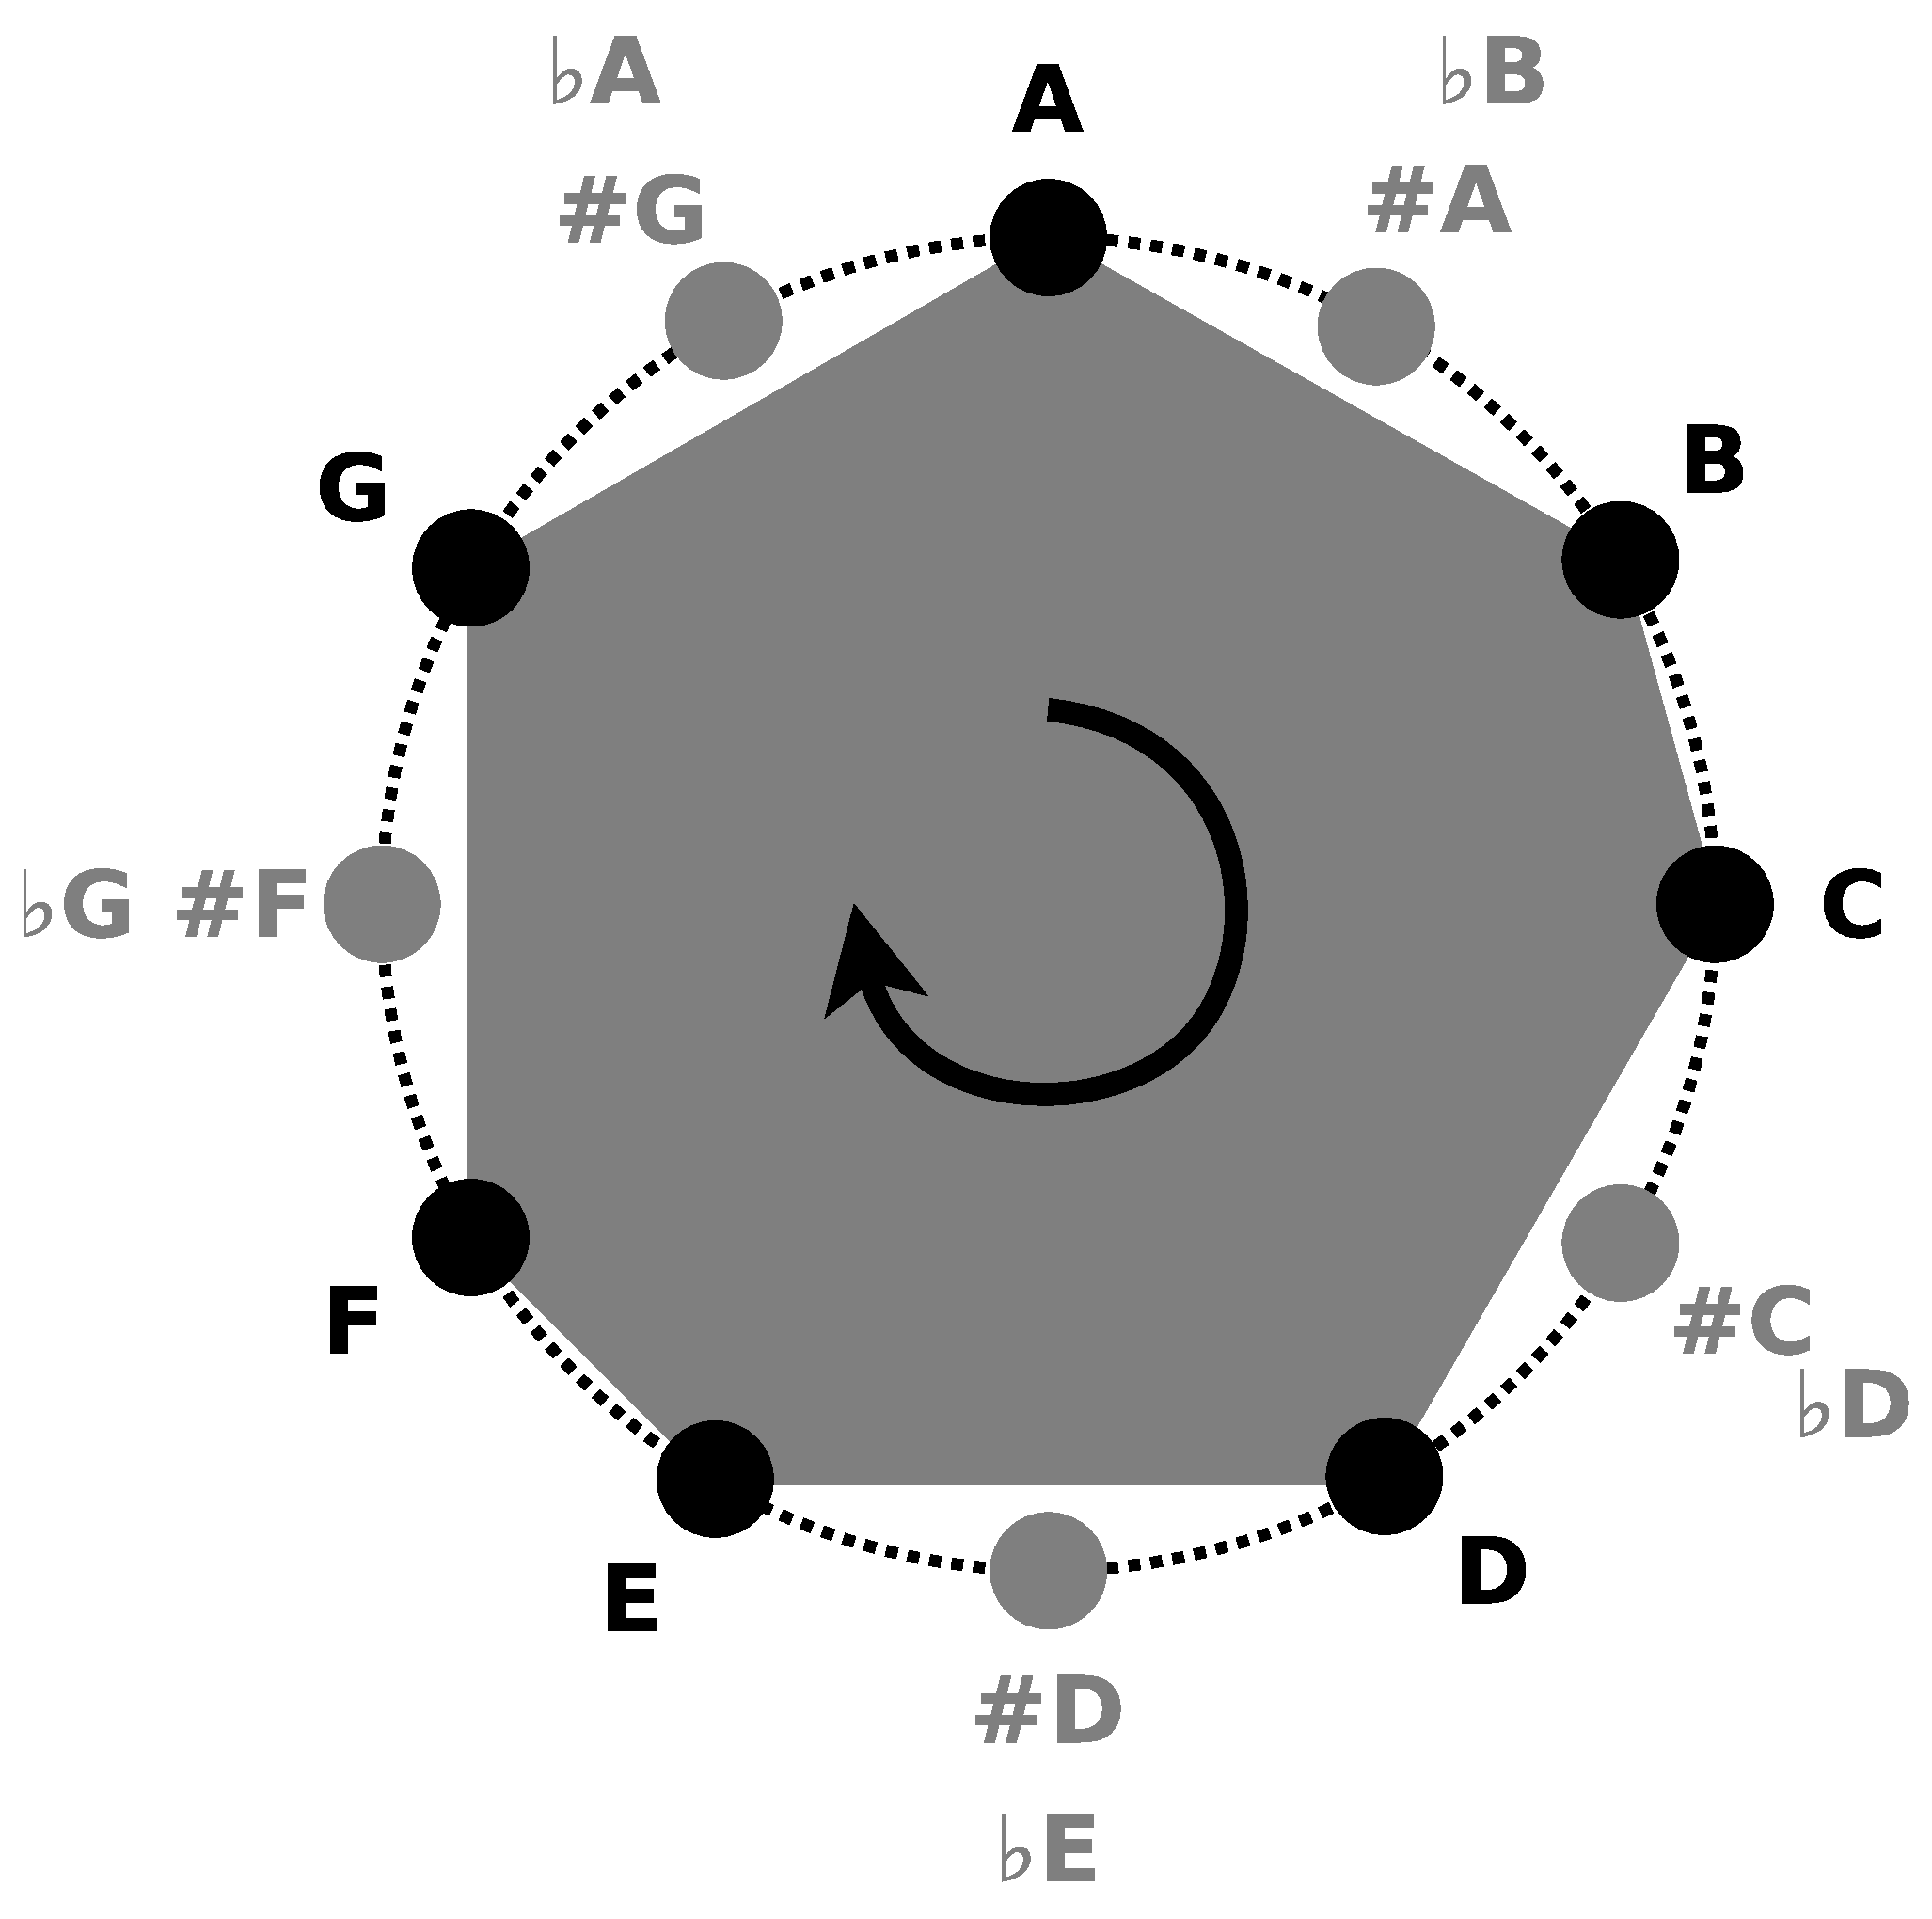
\includegraphics[width=0.65\textwidth]{chapters/cap-musica-basica/circulonotas.eps}
        \caption{Representação cíclica das distancias das notas musicais.}
        \label{fig:circulonotas}
    \end{figure}

Adicionalmente, na Figura \ref{fig:circulonotas}, 
está representada a escala diatônica com uma figura geométrica de 6 lados, 
colorido em cinza; e a escala cromática está representada com um circulo de linha pontuada.



     %[OK]
%%%%%%%%%%%%%%%%%%%%%%%%%%%%%%%%%%%%%%%%%%%%%%%%%%%%%%%%%%%%%%%%%%%%%%%%%%%%%%%%
\section{Tipos de pauta}
\label{sec:tipospauta}

%%%%%%%%%%%%%%%%%%%%%%%%%%%%%%%%%%%%%%%%%%%%%%%%%%%%%%%%%%%%%%%%%%%%%%%%%%%%%%%%
%%%%%%%%%%%%%%%%%%%%%%%%%%%%%%%%%%%%%%%%%%%%%%%%%%%%%%%%%%%%%%%%%%%%%%%%%%%%%%%%
\subsection{Pauta ou Pentagrama}\index{Pauta}
\label{sec:pauta}
A pauta está representada por 5 linhas paralelas e horizontais, 
as figuras musicais podem ocupar as linhas ou um lugar médio, entre elas;
de modo que a parte das figuras que indica a posição delas na pauta é o círculo branco ou preto, dependendo do caso.
Adicionalmente, lugares fora da pauta podem ser usados; 
para este propósito, linhas adicionais e parcialmente desenhadas, 
serão colocadas abaixo da figura musical \cite[pp. 10]{cardoso1973curso},
como é mostrado na Figura \ref{fig:abc-pauta5}.
\begin{figure}[H]
\centering
\begin{abc}[name=abc-pauta5]
% abcm2ps pauta5.abc  -O pauta5.ps
% ps2epsi pauta5.ps pauta5.eps
%
X: 1 % start of header
K: none stafflines=5 %K: C %% Escala de C mayor %
M: none % M: 2/4
%T: Contratempo num compasso binário
V:1 clef=none stem=up name="Pauta"   sname="Pauta"
%
[V:1] C8 D8 E8 F8 G8 A8 B8 C'8 D'8 E'8 F'8 G'8 A'8
\end{abc}
\caption{Pauta com 5 linhas e figuras musicais mostrando algumas posições usáveis.}
\label{fig:abc-pauta5}
\end{figure}
A ordem de leitura das figuras musicais na pauta é de esquerda a direita,
e indica o avanço  do tempo;
as posições das linhas indicam um ordem crescente na altura do som que representam as figuras,
contando desde a linha inferior ate a superior. Nesse sentido, 
uma pauta é semelhante a um espectrograma, onde o eixo X representa o tempo,
o eixo Y representa a frequência, e a figuras colocadas em distintas posições do plano XY, descrevem
o comportamento do sonido nesses dois âmbitos. Assim, a Figura \ref{fig:abc-pauta5}
representa um conjunto de 13 sonidos, cada um com a mesma duração; 
porem, articulado com diferentes alturas e em ordem crescente, 
desde um sonido grave ate um sonido mais agudo.
%\begin{remark}
%As linhas da pauta se contam de abaixo para acima.
%As figuras musicais, se leem de esquerda direita, para que corresponda com o sentido do avanço do tempo.
%\end{remark}


Por outro lado, se as figuras musicais podem ocupar varias posições entre as linhas da pauta,
pois estos lugares representam alturas diferentes do som; então, 
as pausas  ou silêncios não precisam desta característica,
pelo qual os símbolos que representam os silêncios tem uma posição fixa na pauta,
como pode ser visto na Figura \ref{fig:abc-pautasilencio}.
\begin{figure}[h]
\centering
\begin{abc}[name=abc-pautasilencio]
% abcm2ps pautasilencio.abc  -O pautasilencio.ps
% ps2epsi pautasilencio.ps pautasilencio.eps
%
X: 1 % start of header
K: none stafflines=5 %K: C %% Escala de C mayor %
M: none % M: 2/4
%T: Contratempo num compasso binário
V:1 clef=none name="Pauta"   sname="Pauta"
%
[V:1] z8 z4 z2 z1 z/2 z/4 G8 A4 B2 C'1 D'/2 E'/4 
\end{abc}
\caption{Pauta com 5 linhas e silêncios musicais mostrando algumas posições usáveis.}
\label{fig:abc-pautasilencio}
\end{figure}

O ponto mais interessante, é ver a diferencia do uso  da pausa de mínima e da pausa de semibreve,
dado que estes dois tipos de pausa usam o mesmo símbolo, porem em distintas posições.
Na Figura \ref{fig:abc-pautasilencio} a pausa de semibreve, 
está colocada em primeiro lugar desde a esquerda da pauta,
e o símbolo está desenhado unido a parte baixa de uma linha da pauta.
Por outro lado, a pausa de mínima está desenhada no segundo lugar da pauta,
contando desde a esquerda, e se desenha unida à parte de acima de uma linha da pauta.
Estos dois simbolo podem estar desenhados em duas linhas diferentes, 
como no exemplo da Figura \ref{fig:abc-pautasilencio}, ou na mesma linha.

\subsubsection{As claves na pauta}
\label{subsubsec:clavespauta}
A clave, como símbolo, 
se coloca ao inicio da pauta, 
e serve para indicar as alturas das notas na pauta \cite[pp. 179]{apel1969harvard} \cite[pp. 10]{cardoso1973curso}.
Existem 3 tipos de claves\footnote{E varias posições para estas, porem aqui veremos as mas basicas.} que podem ser usadas na pauta, 
assim temos: 
\begin{description}
\item [Clave sol:] Representada pelo símbolo 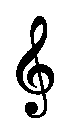
\includegraphics[height=14pt]{chapters/cap-musica-basica/G-clef.eps}. 
A posição donde esta clave se assine indica o lugar onde se localiza uma nota sol. 
\begin{example}
Na Figura \ref{fig:abc-clavesol} podemos ver à clave de sol assinada sobre a segunda linha da pauta,
indicando que esta linha representa a nota sol.
Adicionalmente uma nota sol usando uma  semibreve é colocada.
\end{example} 
\item [Clave de fá:] Representada pelo símbolo 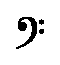
\includegraphics[height=10pt]{chapters/cap-musica-basica/FClef.eps}. 
A posição donde essa clave se assine indica o lugar onde se localiza uma nota fá.
\begin{example}
Na Figura \ref{fig:abc-clavefa} podemos ver à clave de fá assinada sobre a quarta linha da pauta,
indicando que essa linha representa a nota fá.
Adicionalmente uma nota fá usando uma  semibreve é colocada.
\end{example} 
\item [Clave de dó:] Representada pelo símbolo 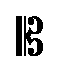
\includegraphics[height=10pt]{chapters/cap-musica-basica/CClef.eps}.
A posição donde esta clave se assine indica o lugar onde se localiza uma nota dó.
\begin{example}
Na Figura \ref{fig:abc-clavedo} podemos ver à clave de dó assinada sobre a terceira linha da pauta,
indicando que essa linha representa a nota dó.
Adicionalmente uma nota dó usando uma  semibreve é colocada.
\end{example} 
\end{description}
%%%
\begin{figure}[h]
    \centering
\begin{subfigure}[c]{0.25\textwidth}
\begin{abc}[name=abc-clavesol]
% abcm2ps clavesol.abc  -O clavesol.ps
% ps2epsi clavesol.ps clavesol.eps
%
X: 1 % start of header
K: C stafflines=5 %K: C %% Escala de C mayor %
M: none % M: 2/4
%T: Contratempo num compasso binário
V:1 clef=treble %name="Pauta com clave de sol"   sname="Pauta com clave de sol"
%
[V:1] G8
\end{abc}
\caption{Clave de sol com uma semibreve colocada em sol.}
\label{fig:abc-clavesol}
\end{subfigure}
~ %
\begin{subfigure}[c]{0.25\textwidth}
\begin{abc}[name=abc-clavefa]
% abcm2ps clavesfa.abc  -O clavefa.ps
% ps2epsi clavefa.ps clavefa.eps
%
X: 1 % start of header
K: C stafflines=5 %K: C %% Escala de C mayor %
M: none % M: 2/4
%T: Contratempo num compasso binário
V:1 clef=bass %name="Pauta com clave de fá"   sname="Pauta com clave de fá"
%
[V:1] F,8  
\end{abc}
\caption{Clave de fá com uma semibreve colocada em fá.}
\label{fig:abc-clavefa}
\end{subfigure}
~ %
\begin{subfigure}[c]{0.25\textwidth}
\begin{abc}[name=abc-clavedo]
% abcm2ps clavesfa.abc  -O clavedo.ps
% ps2epsi clavedo.ps clavedo.eps
%
X: 1 % start of header
K: C stafflines=5 %K: C %% Escala de C mayor %
M: none % M: 2/4
%T: Contratempo num compasso binário
V:1 clef=C %name="Pauta com clave de fá"   sname="Pauta com clave de fá"
%
[V:1] C8 
\end{abc}
\caption{Clave de dó com uma semibreve colocada em dó.}
\label{fig:abc-clavedo}
\end{subfigure}
    \caption{Tipos de claves}\label{fig:allclaves}
\end{figure}



\subsubsection{As claves e a escala diatonica}
Conhecida as definições das claves, e da \hyperref[sec:pos:Diatonica]{\textbf{escala diatônica}}, 
podemos misturar estes dois conceitos para conhecer a posição de todas as notas na pauta
\cite[pp. 10]{cardoso1973curso} \cite[pp. 14]{medteoria}.

Por exemplo, as pautas desenhadas na Figura \ref{fig:allnotesclaves} 
contem duas duas oitavas cada uma, centradas em dó, e com notas escritas usando semibreves.
\begin{figure}[h]
    \centering
\begin{abc}[name=abc-clavenotessol]
% abcm2ps clavenotessol.abc  -O clavenotessol.ps
% ps2epsi clavenotessol.ps clavenotessol.eps
%
X: 1 % start of header
K: C stafflines=5 %K: C %% Escala de C mayor %
M: none % M: 2/4
%T: Contratempo num compasso binário
V:1 clef=treble %name="Pauta com clave de sol"   sname="Pauta com clave de sol"
%
[V:1] "dó"C,8 "ré"D,8 "mi"E,8 "fá"F,8  "sol"G,8 "lá"A,8 "si"B,8 "dó"C8 "ré"D8 "mi"E8 "fá"F8  "sol"G8 "lá"A8 "si"B8 "dó"C'8 
\end{abc}

\begin{abc}[name=abc-clavenotesfa]
% abcm2ps clavenotesfa.abc  -O clavenotesfa.ps
% ps2epsi clavenotesfa.ps clavenotesfa.eps
%
X: 1 % start of header
K: C stafflines=5 %K: C %% Escala de C mayor %
M: none % M: 2/4
%T: Contratempo num compasso binário
V:1 clef=bass %name="Pauta com clave de fá"   sname="Pauta com clave de fá"
%
[V:1] C,8 D,8 E,8 F,8 G,8 A,8 B,8 C8 D8 E8 F8 G8 A8 B8 C'8 
\end{abc}

\begin{abc}[name=abc-clavenotesdo]
% abcm2ps clavenotesfa.abc  -O clavenotesdo.ps
% ps2epsi clavenotesdo.ps clavenotesdo.eps
%
X: 1 % start of header
K: C stafflines=5 %K: C %% Escala de C mayor %
M: none % M: 2/4
%T: Contratempo num compasso binário
V:1 clef=C %name="Pauta com clave de fá"   sname="Pauta com clave de fá"
%
[V:1] C,8 D,8 E,8 F,8 G,8 A,8 B,8 C8 D8 E8 F8 G8 A8 B8 C'8 
\end{abc}
    \caption{Tipos de claves}\label{fig:allnotesclaves}
\end{figure}
Na pauta com clave de sol, 
se distingue como as notas da oitava mais alta estão bem posicionadas na pauta;
porem, as notas da oitava inferior precisam linhas adicionais para serem representadas,
o que dificultará, ou não deixará elegante a leitura dos elementos na pauta.
Podemos ver um caso similar, pero ao contrario, com a pauta que usa uma clave de fá;
nela, as notas da primeira oitava estão comodamente representadas dentro da pauta;
porem, as da oitava superior precisam linhas adicionais.
Finalmente, a notas escritas usando a clave de dó, estão bem centradas,
para notas com alturas intermédias e só fica fora da pauta as duas notas mais agudas e as duas mais graves.

A primeira vista poderia parecer mais vantajosa a clave de do, 
porem isto acontece só porque a nota central que queremos representar é um dó,
teríamos uma vantagem similar na clave de sol, se usaremos uma nota central em si,
ou a vantagem a teríamos na clave de fá, se usaremos uma nota central em ré. 
Na prática, escolher entre
uma clave u outra dependerá da melodia que queiramos encaixar na pauta.
Porem existe uma combinação muito usada na musica para piano, 
que é usar uma clave de sol pra descrever as melodias a serem tocadas pela mão direita,
e usar uma clave de fá, para as que serão tocadas pela mão esquerda; 
isto é conveniente devido a que se olhamos o dó central nessas claves, 
na Figura \ref{fig:allnotesclaves}, 
poderemos observar que esta nota se sai das linhas da pauta, 
justo para entrar nas linhas da pauta da outra mão.

%%%%%%%%%%%%%%%%%%%%%%%%%%%%%%%%%%%%%%%%%%%%%%%%%%%%%%%%%%%%%%%%%%%%%%%%%%%%%%%%
%%%%%%%%%%%%%%%%%%%%%%%%%%%%%%%%%%%%%%%%%%%%%%%%%%%%%%%%%%%%%%%%%%%%%%%%%%%%%%%%
\subsection{Pauta de percussão}\index{Pauta!Pauta de Percussão}

Existem varias formas de representar as pautas para percussão, 
estas são diferenciadas do pentagrama, devido a que na percussão, 
na maioria dos casos não se tem controle da \hyperref[sec:pos:Duracion]{\textbf{duração}} do som;
e sim se tem, do momento em que este será articulado. Em outros casos,
pode estar desabilitada a possibilidade de mudar a \hyperref[sec:pos:Altura]{\textbf{altura}} dos sons;
pelo que não se necessitam linhas pra representar estas alturas.
Assim, as pautas de percussão estarão optimizadas, em cada caso, 
para mostrar com simplicidade o ritmo que se deseja interpretar.

\subsubsection{A clave de percussão}
Também chamada \textbf{clave neutral} ou \textbf{clave de ritmos}, 
porque é usada por percussionistas, bateristas, 
ou usada para qualquer instrumento que produz um som que não tem uma altura definida \cite[pp. 51]{harnum2009basic}.
Asim, esta clave indica que a pauta mostra ritmos e modos de tocar um instrumento, 
e não indica as alturas das notas, 
como outras claves mostradas na Seção \ref{subsubsec:clavespauta}.
Podemos achar dois símbolos equivalentes para representar esta clave, 
estes são 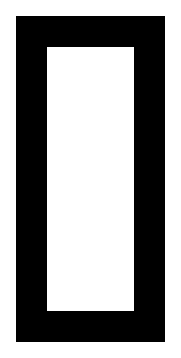
\includegraphics[height=10pt]{chapters/cap-musica-basica/P1-clef.eps}
e 
\includegraphics[height=10pt]{chapters/cap-musica-basica/P2-clef.eps}.
Entre os instrumentos que usam esta clave temos:
o tambourine, o triangulo, o pandeiro, etc.
A Figura \ref{fig:allpercusionclaves} mostra algumas formas de usar a clave de percussão,
sendo formas equivalentes, as mostradas na Figura \ref{fig:abc-claveperczero} e a Figura \ref{fig:abc-clavepercuma}.

\begin{figure}[h]
    \centering 
\begin{subfigure}[c]{0.24\textwidth}
\begin{abc}[name=abc-clavepercusion1]
% abcm2ps clavepercusion1.abc  -O clavepercusion1.ps
% ps2epsi clavepercusion1.ps clavepercusion1.eps
%
X: 1 % start of header
K: C stafflines=0 %K: C %% Escala de C mayor %
M: none % M: 2/4
%T: Contratempo num compasso binário
V:1 clef=perc stem=up %name="Pauta com clave de fá"   sname="Pauta com clave de fá"
%
[V:1] B1 B1 B2 B1 B2   
\end{abc}
\caption{Clave de percussão sem linhas, indicando que só existe um modo de tocar o instrumento.}
\label{fig:abc-claveperczero}
\end{subfigure}
~%
\begin{subfigure}[c]{0.24\textwidth}
\begin{abc}[name=abc-clavepercusion2a]
% abcm2ps clavepercusion2a.abc  -O clavepercusion2a.ps
% ps2epsi clavepercusion2a.ps clavepercusion2a.eps
%
X: 1 % start of header
K: C stafflines=1 %K: C %% Escala de C mayor %
M: none % M: 2/4
%T: Contratempo num compasso binário
V:1 clef=perc stem=up %name="Pauta com clave de fá"   sname="Pauta com clave de fá"
%
[V:1] B1 B1 B2 B1 B2   
\end{abc}
\caption{Clave de percussão com uma linha e um modo de tocar o instrumento.}
\label{fig:abc-clavepercuma}
\end{subfigure}
~%
\begin{subfigure}[c]{0.24\textwidth}
\begin{abc}[name=abc-clavepercusion2]
% abcm2ps clavepercusion2.abc  -O clavepercusion2.ps
% ps2epsi clavepercusion2.ps clavepercusion2.eps
%
X: 1 % start of header
K: C stafflines=1 %K: C %% Escala de C mayor %
M: none % M: 2/4
%T: Contratempo num compasso binário
V:1 clef=perc stem=up %name="Pauta com clave de fá"   sname="Pauta com clave de fá"
%
[V:1] A1 C'1 A2 C'1 A2   
\end{abc}
\caption{Clave de percussão com uma linha e dois modos de tocar o instrumento.}
\label{fig:abc-clavepercum2}
\end{subfigure}
~%
\begin{subfigure}[c]{0.24\textwidth}
\begin{abc}[name=abc-clavepercusion3]
% abcm2ps clavepercusion3.abc  -O clavepercusion3.ps
% ps2epsi clavepercusion3.ps clavepercusion3.eps
%
X: 1 % start of header
K: C stafflines=5 %K: C %% Escala de C mayor %
M: none % M: 2/4
%T: Contratempo num compasso binário
V:1 clef=perc stem=up %name="Pauta com clave de fá"   sname="Pauta com clave de fá"
%
[V:1] A1 B1 G2 C'1 F2   
\end{abc}
\caption{Clave de percussão com cinco linhas e vários modos de tocar o instrumento.}
\label{fig:abc-claveperccinco}
\end{subfigure}
    \caption{Usos da clave de percussão}\label{fig:allpercusionclaves}
\end{figure}


\begin{example}[Pauta para caxixi] ~

\begin{minipage}{0.745\textwidth}
Para escrever um ritmo para um caxixi, 
podemos usar uma pauta como na Figura \ref{fig:abc-claveperczero} ou na Figura \ref{fig:abc-clavepercuma}, 
onde  cada figura musical indica um movimento do caxixi.
\end{minipage}~~
\begin{minipage}{0.1\textwidth}
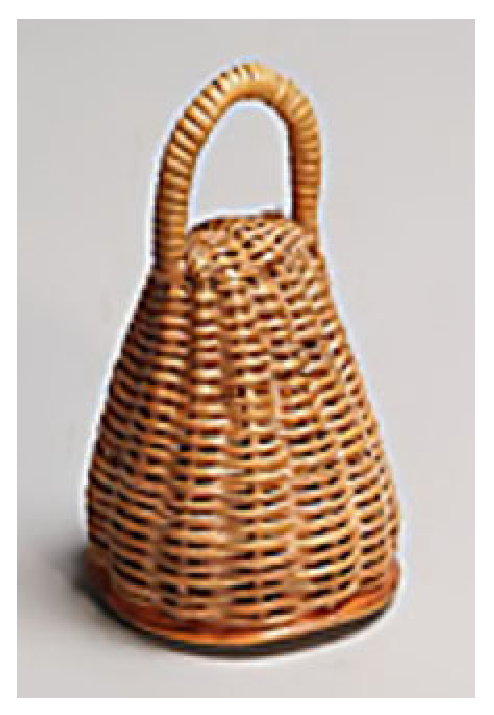
\includegraphics[width=\textwidth]{chapters/cap-musica-basica/caxixi.eps}
\end{minipage}
\end{example} 

\begin{example}[Pauta para agogô] ~

\begin{minipage}{0.595\textwidth}
Para escrever um ritmo para um agogô, 
podemos usar uma pauta como na Figura \ref{fig:abc-clavepercum2}, 
onde  as figuras musicais desenhadas acima da linha indicam um batimento para um som agudo,
e as desenhadas abaixo da linha um batimento para um som grave.
\end{minipage}~~
\begin{minipage}{0.25\textwidth}
\includegraphics[width=\textwidth]{chapters/cap-musica-basica/agogo.eps}
\end{minipage}
\end{example} 

\begin{example}[Pauta para vários instrumentos de percussão] ~

\begin{minipage}{0.845\textwidth}
Se temos um conjunto de instrumentos de percussão, 
e queremos escrever um ritmo, poderíamos usar uma representação como na Figura \ref{fig:abc-claveperccinco},
e atribuir uma ou mais linhas da pauta a cada um dos instrumentos
\end{minipage}
\end{example} 



\subsubsection{Notação para instrumentos que usam golpes secos}
Instrumentos musicais nos quais só podemos controlar o inicio do som, e não a duração dos mesmos, 
devem ser escritos na pauta com figuras musicais longas, 
é dizer figuras musicais que preencham os silêncios posteriores a execução do sonido;
um exemplo disto pode ser visto na Figura \ref{fig:clavepercusiondryall}.
Assim, obteremos uma leitura da pauta mais clara, 
numa representação como na Figura \ref{fig:abc-clavepercusiondry2}, que usa figuras longas.
Por outro lado agregaremos complexidade à leitura numa representação como na Figura \ref{fig:abc-clavepercusiondry1},
pelo qual se desaconselha seu uso \cite[pp. 289]{gould676behind}.
\begin{figure}[h]
    \centering 
\begin{subfigure}[c]{0.45\textwidth}
\begin{abc}[name=abc-clavepercusiondry1]
% abcm2ps clavepercusiondry1.abc  -O clavepercusiondry1.ps
% ps2epsi clavepercusiondry1.ps clavepercusiondry1.eps
%
X: 1 % start of header
K: C stafflines=1 %K: C %% Escala de C mayor %
M: none % M: 2/4
%T: Contratempo num compasso binário
V:1 clef=perc stem=up %name="Pauta com clave de fá"   sname="Pauta com clave de fá"
%
[V:1] B1/2 z1/2 B1/2 z1/2 B1/2 z3/2 B1/2 z1/2 B1/2 z3/2 B1/2 z1/2 
\end{abc}
\caption{Notação de percussão usando figuras cortas.}
\label{fig:abc-clavepercusiondry1}
\end{subfigure}
~%
\begin{subfigure}[c]{0.45\textwidth}
\begin{abc}[name=abc-clavepercusiondry2]
% abcm2ps clavepercusiondry2.abc  -O clavepercusiondry2.ps
% ps2epsi clavepercusiondry2.ps clavepercusiondry2.eps
%
X: 1 % start of header
K: C stafflines=1 %K: C %% Escala de C mayor %
M: none % M: 2/4
%T: Contratempo num compasso binário
V:1 clef=perc stem=up %name="Pauta com clave de fá"   sname="Pauta com clave de fá"
%
[V:1] B1 B1 B2 B1 B2 B1 
\end{abc}
\caption{Notação de percussão usando figuras longas.}
\label{fig:abc-clavepercusiondry2}
\end{subfigure}
    \caption{Duração das figuras em instrumentos que usam golpes secos.}\label{fig:clavepercusiondryall}
\end{figure}

\subsubsection{O sistema de notação monolinear}
Este sistema foi criado pelo baterista suiço, Dr. Fritz Berger, em 1928. 
Ele o chamou ``the monolinear notation system'', 
de modo que seu sistema utilizava uma única linha na pauta, na sua definição,
a parte de acima da linha representava a mão direita (para a bateria), e
a parte de abaixo da linha a mão esquerda.
Assim, era mais fácil ler os ritmos, deixando claro que mão devia fazer uma determinada ação
\cite[pp. 148]{beck1995encyclopedia} \cite[pp. 332]{dean2012drum}.
Um exemplo deste sistema pode ser visto na Figura \ref{fig:abc-clavepercum2}.

\subsubsection{A notação em grade}
A notação em grade é também chamado como ``drum machine tabulature'' \cite{badness1991drum} ou
``grid notation'' \cite{bardet1985200}. Este tipo de notação tem uma representação como na Figura \ref{fig:gridnotation1},
onde cada linha indica o uso de um instrumento de percussão, 
e cada caixa na linha representa uma unidade de tempo, neste caso temos 16 unidades de tempo.
Para o caso de instrumentos com um único modo de ser articulado, como na Figura \ref{fig:abc-clavepercusiondry2},
as caixas pretas representam tempos onde existe o comando para a execução do instrumento,
consequentemente as caixas brancas indicam uma inação na execução do instrumento.
Assim, a representação em grade mostrada na Figura \ref{fig:gridnotation1} 
é equivalente à Figura \ref{fig:abc-clavepercusiondry2}.
\begin{figure}[h]
    \centering 
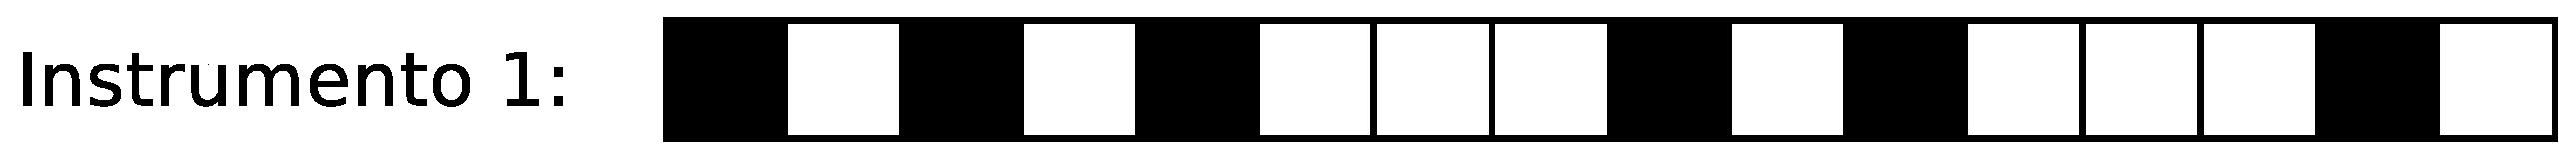
\includegraphics[width=0.7\textwidth]{chapters/cap-musica-basica/gridnotation.eps}
    \caption{Notação em grade.}\label{fig:gridnotation1}
\end{figure}

Também existe a possibilidade de ter uma representação em grade, para instrumentos, 
com vários modos de ser articulados, para este efeito podem ser usadas duas ou mais linhas,
ou cada linha poder ter mais de dois símbolos por elemento.
Por exemplo, a Figura \ref{fig:gridnotation2a} representa a notação em grade usando
varias linhas por instrumento. A Figura \ref{fig:gridnotation2b} é equivalente 
a representação mostrada na Figura \ref{fig:gridnotation2a}, porem usando vários símbolos por elemento.

\begin{figure}[h]
    \centering 
\begin{subfigure}[c]{0.7\textwidth}
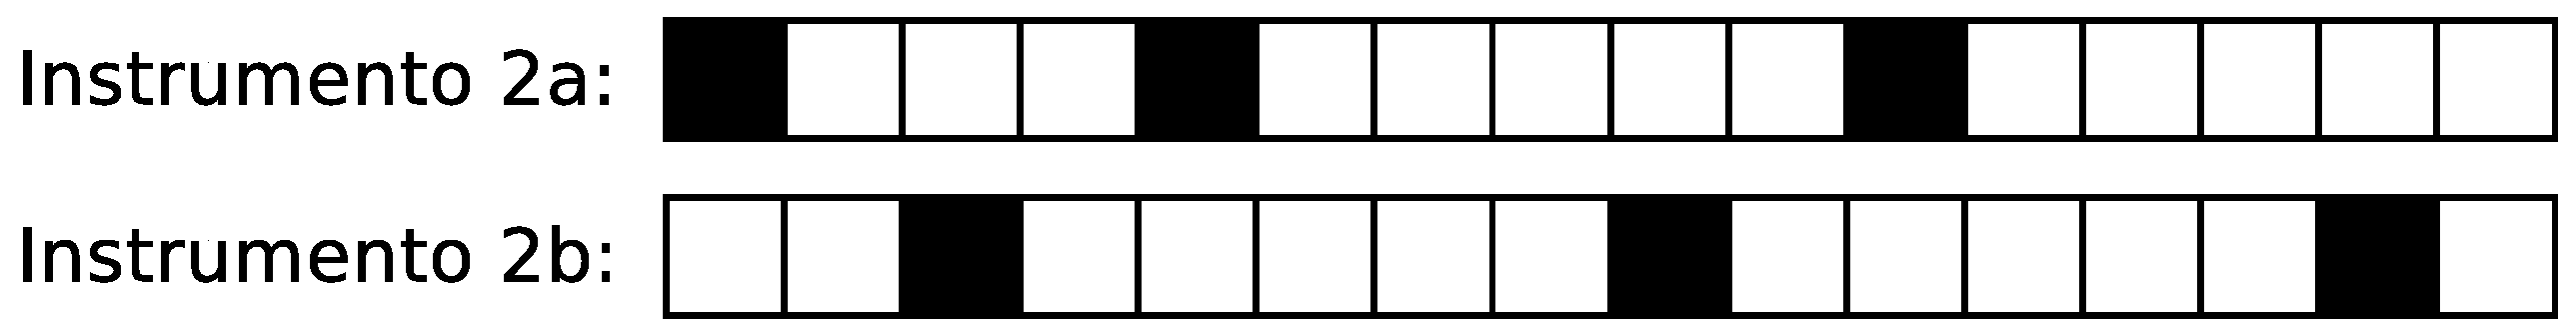
\includegraphics[width=\textwidth]{chapters/cap-musica-basica/gridnotation2a.eps}
\caption{Notação usando várias linhas por instrumento.}
\label{fig:gridnotation2a}
\end{subfigure}
~%
\begin{subfigure}[c]{0.7\textwidth}
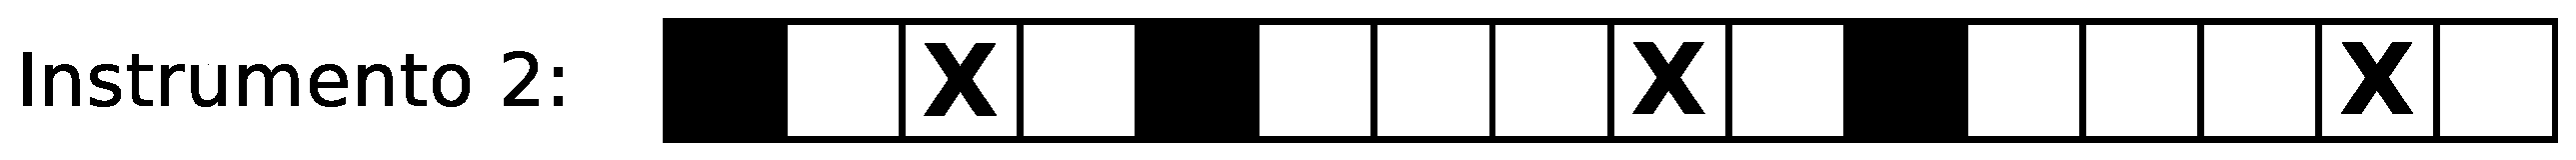
\includegraphics[width=\textwidth]{chapters/cap-musica-basica/gridnotation2b.eps}
\caption{Notação usando vários símbolos por elemento em cada instrumento.}
\label{fig:gridnotation2b}
\end{subfigure}
    \caption{Notação em grade para instrumentos com dois modos de execução.}\label{fig:gridnotation2}
\end{figure}

%\cite[pp. 121]{feist2017berklee}


\begin{comment}
\subsubsection{The musical notation of percusion}
Revisar  \cite[pp. 70]{harnum2009basic}

Figura \ref{fig:abc-musicalperc}
\begin{figure}[H]
\centering
\begin{abc}[name=abc-musicalperc]
% abcm2ps musicalperc.abc  -O musicalperc.ps
% ps2epsi musicalperc.ps musicalperc.eps
%
X:1
T:Drum Key
M:
L:1/4
K:C clef=perc
"^Bass"F|"^Snare"c|"^High tom"e|"^Mid tom"d|"^Low tom"B|"^Floor tom"A|
"^Cymbal"^b|"^Crash"^a|"^Hi-hat"^g|"^Ride"^f|"^Hi-hat Pedal"^D|]

\end{abc}
\caption{Figuras e pausas}
\label{fig:abc-musicalperc}
\end{figure}
\end{comment}


        %
%%%%%%%%%%%%%%%%%%%%%%%%%%%%%%%%%%%%%%%%%%%%%%%%%%%%%%%%%%%%%%%%%%%%%%%%%%%%%%%%
\section{Compasso}\index{Compasso}
\label{sec:compaso}

\begin{description}
\item[Compasso:] \label{def:Compasso} Se define compasso (``measure'' em inglês)
como uma agrupação de \hyperref[sec:Tempo]{\textbf{tempos}} regulares na sua duração (também chamados de batimentos ou pulsos),
onde o primeiro destes tempos normalmente é o mais acentuado,
porem a regularidade nesta acentuação pode mudar pela aparição de elementos como \hyperref[sec:contratempo]{\textbf{contratempos}}, 
\hyperref[sec:sincopa]{\textbf{sincopas}}, ou enfases em algumas notas  \cite[pp. 513]{apel1969harvard}. 
O número de \hyperref[sec:Tempo]{\textbf{tempos}} no compasso pode ser, dois, trés, quatro, ou ocasionalmente 5 ou mais;
assim, estes tempos são usados como a unidade de medida (temporal) do compasso.
Para diferenciar o inicio e o final dos compassos, 
estes são separados por barras verticais. 
O esquema básico dos valores das notas dentro de um compasso é chamado de \hyperref[def:Metrica]{\textbf{métrica}}  ou \hyperref[def:Metrica]{\textbf{metro}}.
\begin{example}
Na Figura \ref{fig:abc-exemplocompasso1} podemos ver 4 compassos separados por barras verticais.
A quantidade de figuras musicais dentro do compasso varia, 
porem todos todos os compassos tem uma duração de  1 \Halb~(uma mínima).
\end{example}
 
\begin{figure}[h]
\centering
\begin{abc}[name=abc-exemplocompasso1]
% abcm2ps exemplocompasso1.abc  -O exemplocompasso1.ps
% ps2epsi exemplocompasso1.ps exemplocompasso1.eps
%
X: 1 % start of header
K: none stafflines=0 %K: C %% Escala de C mayor %
M: 2/4
%T: Contratempo num compasso binário
V:1 clef=perc stem=up name="Ritmo 1"   sname="Ritmo 1"
%
[V:1] | B2 B1 B1| B2 B1 B1 | B2 B1 B1 | B2 z2  |
%       
\end{abc}
\caption{Ritmo usando 4 compassos.}
\label{fig:abc-exemplocompasso1}
\end{figure}

\item[Métrica:] \label{def:Metrica} 
A métrica ou o metro  (``meter'' em inglês) é
um padrão de unidades temporais regulares (também chamados de \hyperref[sec:Tempo]{\textbf{tempos}}), 
sobre o qual uma peça musical ou uma seção dela é medida ou organizada;
uma agrupação métrica completa se denomina \hyperref[def:Compasso]{\textbf{compasso}} \cite[pp. 947]{latham2017diccionario} \cite[pp. 523]{apel1969harvard}.
A métrica é indicada geralmente por uma fração, por exemplo:
${2}/{2}$ , ${3}/{4}$ , ${4}/{4}$, etc; 
em português esta fração é chamada de \hyperref[def:FormulaCompasso]{\textbf{fórmula do compasso}}.
Assim, a métrica de uma porção de peça musical nos indica como os \hyperref[sec:Tempo]{\textbf{tempos}} são distribuídos nos compassos,
e consequentemente como serão acentuados cada um destes tempos. Isto será mais evidente, mais adiante, 
quando sejam explicadas as caraterísticas dos compassos binários, ternários, quaternários, etc.
\begin{example}
A Figura \ref{fig:abc-exemplocompasso1} mostra 4 compassos com a mesma métrica;
é dizer, igual acentuação e igual número de tempos por compasso.
Neste caso a acentuação é regular dado que todos os compassos usam a mesma formula de compasso, (2/4), 
e não existe nenhuma grafia especial que tire a regularidade das acentuações;
de modo que todos os compassos estão acentuados no primeiro \hyperref[sec:Tempo]{\textbf{tempo}}.
\end{example}

\begin{example}
A Figura \ref{fig:abc-exemplometrica1} mostra 4 compassos com duas distintas métricas;
os dois primeiros usam uma métrica (2/4) e os dois últimos uma métrica (3/4).
\end{example}

\begin{figure}[h]
\centering
\begin{abc}[name=abc-exemplometrica1]
% abcm2ps exemplometrica1.abc  -O exemplometrica1.ps
% ps2epsi exemplometrica1.ps exemplometrica1.eps
%
X: 1 % start of header
K: none stafflines=0 %K: C %% Escala de C mayor %
M: 2/4
%T: Contratempo num compasso binário
V:1 clef=perc stem=up name="Ritmo 2"   sname="Ritmo 2"
%
[V:1] | B2 B1 B1| B2 B1 B1 |\
M: 3/4 
B2 B1 B2 B1 | B2 B1 B1 z2  |
%       
\end{abc}
\caption{Ritmo com mudança de métrica.}
\label{fig:abc-exemplometrica1}
\end{figure}

\item[Formula do compasso:] \label{def:FormulaCompasso} 
A fórmula do compasso  (``time signature'' em inglês), também chamado indicador do compasso ou indicador do tempo,
é um símbolo que normalmente se representa por uma fração (com ou sem traço), 
e se escreve ao inicio da peça musical, depois da clave; 
ou de uma forma geral, 
ao inicio de algum compasso para indicar a mudança da \hyperref[def:Metrica]{\textbf{métrica}} na música \cite[pp. 760]{latham2017diccionario}  \cite[pp. 852]{apel1969harvard}.
O numerador, da fórmula do compasso, indica o número de \hyperref[sec:Tempo]{\textbf{tempos}} que compõem cada \hyperref[def:Compasso]{\textbf{compasso}} nessa \hyperref[def:Metrica]{\textbf{métrica}}.
Por outro lado, 
o denominador da formula do compasso nos informa a duração de cada um dos \hyperref[sec:Tempo]{\textbf{tempos}}, 
dos compassos pertencentes a essa \hyperref[def:Metrica]{\textbf{métrica}}.
A Tabela \ref{tab:abc-noteslength} em conjunto com a Tabela \ref{tab:abc-noteslengthbasic}, 
indicam o significado do denominador da fórmula do compasso; 
\begin{table}[h]
\centering
\begin{tabular}{|c|c|c|}
\hline
denominador & Figura  & Duração\\ \hline
\hline
$1$   & \fullnote    & $S$ \\ \hline
$2$ & \halfnote    & $S/2$  \\ \hline
$4$ & \quarternote & $S/4$  \\ \hline
$8$ & \eighthnote  & $S/8$  \\ \hline
\end{tabular}
\caption{Duração e símbolos de algumas figuras musicais.}
\label{tab:abc-noteslength}
\end{table}
onde a primeira coluna mostra o denominador da fórmula,
a segunda coluna mostra as figuras musicais que representam cada um dos \hyperref[sec:Tempo]{\textbf{tempos}} do compasso, e 
a terceira indica a duração da figura musical.
É importante
ressaltar que a duração das figuras musicais é relativa, como pode ser visto
na terceira coluna da Tabela \ref{tab:abc-noteslength}, onde estas estão em função
da duração $S$ da semibreve. 
\begin{example}
A Figura \ref{fig:abc-exemplocompasso1} mostra 4 \hyperref[def:Compasso]{\textbf{compassos}} com uma formula de compasso (2/4).
Isto implica que cada compasso tera 2 tempos, 
representados por figuras musicais de 1/4 de semibreve;
é dizer, cada tempo equivale a uma semínima (\Vier). 
\end{example}
\begin{example}
A Figura \ref{fig:abc-exemplometrica1} mostra 4 \hyperref[def:Compasso]{\textbf{compassos}} usando dois diferentes formulas de compasso.
Sendo que os dois primeiros compassos tem dois tempos cada um, 
e os dois últimos compassos tem 3 tempos cada um.
Em todos os casos, os tempos tem durações de figuras musicais de 1/4 de semibreve;
é dizer, cada tempo equivale a uma semínima (\Vier). 
\end{example}
\begin{example}
Outros exemplos de formula de compasso comumente usadas são:
\begin{itemize}
\item A fórmula $\mathbf{2}/2$ com compassos com uma duração de $\mathbf{2}$\halfnote ~(duas mínimas) e
\item a fórmula $\mathbf{4}/4$ com compassos com uma duração de $\mathbf{4}$\quarternote ~(quatro semínimas). 
\end{itemize}
\end{example}
\end{description}


Se classificamos os compassos por sua \hyperref[def:Metrica]{\textbf{métrica}}, 
os três tipos de compassos mais conhecidos são: 
os \hyperref[subsec:compassobinario]{\textbf{compassos binários}}, 
\hyperref[subsec:compassoternario]{\textbf{ternários}} e 
\hyperref[subsec:compassoquaternario]{\textbf{quaternários}} \cite[pp. 27]{adolfo2002musica}.

\begin{notation}[]
Nas seguintes seções,
serão usadas as seguintes notações de símbolos para designar aos tempos fortes, fracos e semifortes:
\begin{itemize}
\item ``F''  indica que é um tempo forte, 
\item ``sF'' indica que é um tempo semiforte, 
\item ``f''  indica que é um tempo fraco,
\end{itemize}
\end{notation}


\begin{description}
\item[Acentos principais:] \label{def:acentoprincipal} 
São os acentos dos tempos do compasso  \cite[pp. 142]{medteoria}.
Todos os compassos tem um acento primario no primeiro tempo \cite[pp. 24]{crowther2003usted}.
\item[Acentos secundários:] \label{def:acentosecundario} 
São os acentos das subdivisões dos tempos do compasso \cite[pp. 142]{medteoria}.
Todos os compassos com mais de 3 tempos tem além do acento primário um ou mais acentos secundários \cite[pp. 25]{crowther2003usted},
\begin{itemize}
\item Os compassos quaternários tem um acento secundário no terceiro tempo,
\item os compassos com formula do compasso com numerador 6  tem um acento secundário na quarta subdivisão do compasso, e
\item os compassos com formula do compasso com numerador 9  tem    acentos secundários na quarta e sétima subdivisão do compasso.
\end{itemize} 
\end{description}

\begin{remark}
Os termos ``acentuados'' e ``não acentuados'', 
indicam uma medida relativa da \hyperref[sec:pos:Intensidade]{\textbf{intensidade}} do som, 
e em nenhum caso indicam intensidade zero. 
\end{remark}

%%%%%%%%%%%%%%%%%%%%%%%%%%%%%%%%%%%%%%%%%%%%%%%%%%%%%%%%%%%%%%%%%%%%%%%%%%%%%%%%
\subsection{Compasso binário}
\label{subsec:compassobinario}
\index{Compasso!Compasso Binário} O compasso binário ou compasso binário simples,
é uma estrutura que se carateriza por ter compassos com uma  duração de dois \hyperref[sec:Tempo]{\textbf{tempos}},
sendo o primeiro tempo forte (acentuado), e o segundo de tempo fraco (não acentuado)
\cite[pp. 41]{grabner2001teoria} \cite[pp. 66]{adolfo2002musica}\cite[pp. 28]{alves2004teoria}.
Os compassos binários (simples) tem uma fórmula de compasso na forma $2/B$,
onde $B$ pode ser $2$, $4$, $8$, etc. 
\begin{example}
Por exemplo temos, as fórmulas de compassos binários simples: $2/2$, $2/4$, $4/8$,  etc.
\end{example}
\begin{example}
A Figura \ref{compasso:binario}, representa um exemplo de compasso binário simples, 
com fórmula de compasso $2/2$, estes compassos podem ser preenchidos com $2$\halfnote, 
e tempos com uma duração de $S/2$ (uma \halfnote).
Neste caso, podemos ver 3 compassos que são preenchidos com $2$ notas representadas por \halfnote.
Assim, a primeira nota de cada compasso representa um tempo forte (acentuado), e a segunda um tempo fraco (não acentuado).
\end{example}
\begin{figure}[H]
\centering
\begin{abc}[name=abc-compasso1,width=0.70\linewidth]
X: 1 % start of header
K: C % scale: C major
M: 2/2 %meter - compasso
"1ro compasso" G4 F4 |"2do compasso" G4 D4 |"3ro compasso" F4 D4  |
w: F f F f  F f
\end{abc}
\caption{Exemplo de compasso binário (simples).}
\label{compasso:binario}
\end{figure}

Se falamos de forma mais geral, 
podemos ter dois tipos de compassos binários: os simples e os compostos.
Assim, 
para achar a fórmula de um compasso composto, correspondente a um compasso simples (usando quiálteras de três)
usamos a seguinte operação \cite[pp. 74]{alves2004teoria}, 
\begin{equation}\label{eq:comcomposto}
Compasso~simples\times\frac{3}{2}=Compasso~composto.
\end{equation}
De modo que obtemos compassos binários compostos com as seguintes fórmulas de compasso: 
$6/4$, $6/8$, $6/16$, etc.
Os compassos binários compostos, tem a mesma acentuação métrica que os compassos simples,
porem os acentos estão sujeitos a subdivisões ao igual que os tempos. Assim, um compasso binário composto 
tem 2 tempos, um tempo forte (acentuado) no tempo 1 e um tempo fraco (acentuação menor) no tempo 2. 
As subdifiviçoes destes dois tempos se repartirão o acento de forma proporcional,
sendo a primeira parte de cada tempo a mais acentuada \cite[pp. 142]{medteoria} \cite[pp. 7-11]{mascarenhascurso} \cite[pp. 41]{grabner2001teoria}.

\begin{example}
A Figura \ref{compasso:binariocomposto}, representa um exemplo de compasso binário composto, 
com fórmula de compasso $6/4$, 
onde cada tempo tem uma duração de $3S/4$ (uma  \halfnote. $\equiv$ \halfnote + \quarternote). 
No exemplo temos duas linhas, na parte inferior da pauta,  preenchidas com os símbolos ``F'' e ``f'';
a segunda linha representa aos \hyperref[def:acentoprincipal]{\textbf{acentos principais}} dos tempos do compasso, e
a primeira linha representa aos \hyperref[def:acentosecundario]{\textbf{acentos secundarios}}.

O primeiro compasso é preenchido com duas figuras \halfnote~pontuadas, 
representando estas figuras na pauta, um tempo forte (acentuado) e um tempo fraco (menos acentuado),
respetivamente.
O segundo  compasso é preenchido com $6$ figuras \quarternote, 
que representam as subdivisões dos tempos do compasso, de modo que cada tempo é subdividido em 3 partes iguais.
Podemos ver na primeira linha, inferior à pauta, a relação das acentuações nas subdivisões de cada tempo, isto é F-f-f;
e  na segunda linha está representado a relação das acentuações nos tempos, isto é F-f. 
Assim, a primeira subdivisão terá uma acentuação forte (igual a F), 
a quarta subdivisão uma acentuação menor (igual a f) e  resto serão subdivisões sem acentuação (ou menor a f) \cite[pp. 41]{grabner2001teoria} \cite[pp. 19]{phillips2002sight}.
\end{example}
\begin{figure}[H]
\centering
\begin{abc}[name=abc-compasso1c]
X: 1 % start of header
K: C % scale: C major
M: 6/4 %meter - compasso
"1er compasso" G6 F6 |"2do compasso" G2 D2 D2 F2 D2 D2 |
w: ~ ~ F f f F f f 
w: F f F _ _ f _ _ 
\end{abc}
\caption{Exemplo de compasso binário composto.}
\label{compasso:binariocomposto}
\end{figure}
Alguns autores consideram aos compassos quaternários (ex: 4/4, 4/8) como um caso de compasso binário,
chamando eles de compasso binário duplo \cite[pp. 41]{grabner2001teoria}.



%%%%%%%%%%%%%%%%%%%%%%%%%%%%%%%%%%%%%%%%%%%%%%%%%%%%%%%%%%%%%%%%%%%%%%%%%%%%%%%%
\subsection{Compasso ternário}
\label{subsec:compassoternario}
\index{Compasso!Compasso Ternário} O compasso ternário ou compasso ternário simples,
é uma estrutura que se carateriza por ter compassos com trés tempos,
sendo o primeiro tempo forte (acentuado) e os outros dois fracos (não acentuados) 
\cite[pp. 67]{adolfo2002musica}\cite[pp. 30]{alves2004teoria}. 
Os compassos ternários (simples) tem uma fórmula de compasso da forma $3/B$, 
onde $B$ pode ser $2$, $4$, $8$, etc.
\begin{example}
Por exemplo temos, as fórmulas de compassos ternários simples: $3/2$, $3/4$, $3/8$,  etc.
\end{example}
\begin{example}
A Figura \ref{compasso:ternario}, representa um exemplo com 3 compassos ternários (simples), com 
fórmula de compasso $3/4$, onde cada tempo tem uma duração de $S/4$, é dizer uma \quarternote.
Os compassos são preenchidos com $3$ figuras \quarternote, de modo que cada figura musical representa um tempo.
Na Figura \ref{compasso:ternario}  é fácil perceber
que em todos os compassos, só a nota que é executada no tempo 1 é acentuada.
\end{example}
\begin{figure}[H]
\centering
\begin{abc}[name=abc-compasso2,width=0.75\linewidth]
X: 1 % start of header
K: C % scale: C major
M: 3/4 %meter - compasso
"1ro compasso" G2 F2 F2 |"2do compasso" G2 F2 E2 | "3ro compasso" D2 D2  D2  |
w: F f f  F f f   F f f 
\end{abc}
\caption{Exemplo de compasso ternário.}
\label{compasso:ternario}
\end{figure}

São chamados de compassos ternários compostos,  
quando estes tem uma fórmula de compasso como: $9/4$, $9/8$ e $9/16$.
Para gerar estas formulas de compassos compostos a partir de suas versões simples,
se segue a mesma operação descrita na Equação \ref{eq:comcomposto}.

%%%%%%%%%%%%%%%%%%%%%%%%%%%%%%%%%%%%%%%%%%%%%%%%%%%%%%%%%%%%%%%%%%%%%%%%%%%%%%%%
\subsection{Compasso quaternário}
\label{subsec:compassoquaternario}
\index{Compasso!Compasso Quaternário} O compasso quaternário ou compasso quaternário simples,
é uma estrutura que se carateriza por ter compassos com quatro tempos,
sendo o primeiro pulso forte (acentuado), o segundo fraco (não acentuado), 
o terceiro semiforte (acentuado porem menor) e o último fraco (não acentuado) 
\cite[pp. 67]{adolfo2002musica}\cite[pp. 32]{alves2004teoria}. 
Os compassos quaternários (simples) tem uma fórmula de compasso da forma $4/B$, 
onde $B$ pode ser $2$, $4$, $8$, etc.
\begin{example}
Por exemplo temos, as fórmulas de compassos ternários simples: $4/2$, $4/4$, $4/8$,  etc.
\end{example}
\begin{example}
A Figura \ref{compasso:quaternario}, representa um exemplo de 3 compassos quaternários, com 
fórmula de compasso $4/4$, onde cada tempo tem uma duração de $S/4$, é dizer uma \quarternote.
Os compassos são preenchidos com $4$ figuras \quarternote, de modo que cada figura representa um tempo.
Na Figura \ref{compasso:quaternario}  é fácil perceber
que em todos os compassos, só as notas que são executadas no tempo 1 e 3 são acentuadas.
\end{example}
\begin{figure}[H]
\centering
\begin{abc}[name=abc-compasso3]
X: 1 % start of header
K: C % scale: C major
M: 4/4 %meter - compasso
"1ro compasso" G2 D2 F2 D2|"2do compasso" F2 D2 C2 F2 |"3ro compasso"  E2 D2 C2 C2|
w: F f sF f   F f sF f   F f sF f
\end{abc}
\caption{Exemplo de compasso quaternário.}
\label{compasso:quaternario}
\end{figure}

São chamados de compassos quaternários compostos,  
quando estes tem uma fórmula de compasso como: $12/4$, $12/8$ e $12/16$.
Para gerar estes compassos compostos a partir de suas versões simples,
se segue a mesma operação descrita na Equação \ref{eq:comcomposto}.
 

%%%%%%%%%%%%%%%%%%%%%%%%%%%%%%%%%%%%%%%%%%%%%%%%%%%%%%%%%%%%%%%%%%%%%%%%%%%%%%%%

\section{Ligadura}
\index{Música!Ligadura}
\label{sec:ligadura}

A ligadura é uma linha curva que se coloca sobre duas ou mais notas da mesma altura, 
indicando que somente a primeira é articulada, 
e esta tem uma duração equivalente a soma de todas as notas ligadas \cite[pp. 35]{cardoso1973curso}.

\begin{example}
A Figura \ref{fig:total-ligadura} descreve 3 casos de uso de ligadura.
\begin{itemize}
\item Na Figura \ref{fig:abc-ligadura1} pode-se ver que, no primeiro compasso, 
tem-se uma ligadura entre a primeira e a segunda figura musical; 
no segundo compasso tem-se uma representação equivalente ao primeiro compasso; 
porém, usando ponto de aumento.
\item Na Figura \ref{fig:abc-ligadura2} pode-se ver que, no primeiro compasso, 
tem-se ligaduras entre as três primeiras figuras musicais; 
no segundo compasso tem-se uma representação equivalente ao primeiro compasso; 
porém, usando dois pontos de aumento.
\item Na Figura \ref{fig:abc-ligadura3} tem-se um exemplo de uso de ligadura entre figuras musicais de diferentes compassos,
de modo que a duração da última nota, do primeiro compasso, se prolonga ate o segundo compasso.
\end{itemize}
\end{example}


\begin{figure}[!ht]
    \centering
    \begin{subfigure}[b]{0.6\textwidth}
\begin{abc}[name=abc-ligadura1]
X: 1 % start of header
K: C %% Escala de C mayor %
M: 2/4
%T: Contratempo num compasso binário
V:1 clef=G  %name="Ritmo 1"   sname="Ritmo 1"
%
[V:1] | (B2 B1) C1 | B3 C1   |    
\end{abc}
\vspace{-10pt}
\caption{Uso de ligaduras entre duas notas}
\label{fig:abc-ligadura1}
    \end{subfigure}
    ~%add desired spacing between images, e. g. ~, \quad, \qquad, \hfill etc. 
      %(or a blank line to force the subfigure onto a new line)
    \begin{subfigure}[b]{0.6\textwidth}
\begin{abc}[name=abc-ligadura2]
X: 1 % start of header
K: C %% Escala de C mayor %
M: 2/4
%T: Contratempo num compasso binário
V:1 clef=G  %name="Ritmo 1"   sname="Ritmo 1"
%
[V:1] | (A2 (A1) A1/2) C1/2 | A7/2 C1/2  |
\end{abc}
\vspace{-10pt}
\caption{Uso de ligaduras entre três notas.}
\label{fig:abc-ligadura2}
    \end{subfigure}
    ~%add desired spacing between images, e. g. ~, \quad, \qquad, \hfill etc. 
      %(or a blank line to force the subfigure onto a new line)
    \begin{subfigure}[b]{0.6\textwidth}
\begin{abc}[name=abc-ligadura3]
X: 1 % start of header
K: C %% Escala de C mayor %
M: 2/4
%T: Contratempo num compasso binário
V:1 clef=G  %name="Ritmo 1"   sname="Ritmo 1"
%
[V:1] | B3  (G1 | G2) B2  |
\end{abc}
\vspace{-10pt}
\caption{Uso de ligaduras em notas de compassos distintos.}
\label{fig:abc-ligadura3}
    \end{subfigure}
    \caption{Distintos usos da ligadura.}\label{fig:total-ligadura}
\end{figure}


%%%%%%%%%%%%%%%%%%%%%%%%%%%%%%%%%%%%%%%%%%%%%%%%%%%%%%%%%%%%%%%%%%%%%%%%%%%%%%%%
\section{Tempo, acentuação e contagem}
\index{Música!Tempo}
\label{sec:Tempo}

Como já foi sugerido na Seção \ref{sec:compaso}, é chamado de ``tempo''
à pulsação básica que é usada como unidade de medida das composições musicais.
Os tempos ao ser agrupados em compassos podem formar diferentes estruturas como por exemplo: 
\hyperref[subsec:compassobinario]{\textbf{compassos binários}}, 
\hyperref[subsec:compassoternario]{\textbf{ternários}} e 
\hyperref[subsec:compassoquaternario]{\textbf{quaternários}}; que tem uma duração de 2 tempos, 
3 tempos e 4 tempos, respetivamente. 



\subsection{Acentuação dos tempos (parte 2)}
\label{subsec:acentuacion2}
\index{Música!Acentuação}
\index{Música!Tempo!Tempo forte}
\index{Música!Tempo!Tempo fraco}


Mais conceitos sobre a acentuação dos tempos podem ser vistos na Seção \ref{subsec:acentuacion1}.

\begin{notation}[Acentos métricos] Para o melhor entendimento das seguintes seções usaremos algumas notações.
\begin{itemize}
\item A variável $T$ será usada para designar à duração em segundos de cada tempo,
sendo que o valor de $T$ variará dependendo da formula do compasso usada.

\item As subdivisões dos tempos serão designadas com as seguintes variáveis:
\begin{itemize}
\item ``FF'' indica que é a parte forte de um tempo forte,
\item ``Ff'' indica que é a parte fraca de um tempo forte,
\item ``fF'' indica que é a parte forte de um tempo fraco,
\item ``ff'' indica que é a parte fraca de um tempo fraco.
\end{itemize}
\end{itemize}
 
\end{notation}

A formula do compasso de uma peça musical ou uma porção dela, 
nos indica quantos tempos e que duração terão estes tempos no compasso; 
porém, além destas informações, 
a formula do compasso também nos indica o \hyperref[def:acentometrico]{\textbf{acento métrico}} \cite[pp. 70]{cardoso1973curso}; 
é dizer quias serão os tempos fortes, semifortes e fracos no compasso.

\begin{tcbinformation}{Acento métrico}
\index{Música!Acento métrico}
\label{def:acentometrico} 
é constituído pelas acentuações fortes e fracas dos tempos dos compassos, 
a acentuação métrica não precisa ser grafado na pauta;
é dizer, estão sobreintendidos \cite[pp. 141,217]{medteoria}.
\end{tcbinformation} 

\begin{tcbinformation}{Acento dinâmico}
\index{Música!Acento dinâmico}
\label{def:acentodinamico}
 é o acento indicado e grafado pelo compositor na pauta, como meio de expressão;
consequentemente, pelo geral não coincidem com o acento métrico \cite[pp. 217]{medteoria}.
\end{tcbinformation} 


%\item[O acento rítmico] 
%\index{Música!Acento rítmico}
%\label{def:acentoritmico}
%\cite[pp. 217]{medteoria}.

\begin{description}

\item[O tempo forte (F)] 
\index{Música!Tempo forte}
\label{def:tempoforte} 
sempre será o primeiro tempo de cada compasso. 
Um tempo forte não necessita uma grafia especial que indique que este deve ser articulado
com maior \hyperref[sec:pos:Intensidade]{\textbf{intensidade}}; é dizer, com acentuação.

\item[O tempo semiforte (sF)] 
\index{Música!Tempo semiforte}
\label{def:temposemiforte} 
acontece em alguns tipos de compasso, 
como nos compassos quaternários. 
Um tempo semiforte terá uma acentuação menor à do tempo forte, porém maior à de um tempo fraco. 
Este tempo não necessita uma grafia especial que indique que deve ser articulado
com \hyperref[sec:pos:Intensidade]{\textbf{intensidade}}.

\item[O tempo fraco (f)] 
\index{Música!Tempo fraco}
\label{def:tempofraco} 
corresponde a todos os tempos que não sejam né fortes, né semifortes,
de modo que estes tempos não tem acentuação. 
\end{description}~

Uma versão mais simplificada das informações dadas anteriormente, 
pode ser vista na seguinte equação que mostra a relação de \hyperref[sec:pos:Intensidade]{\textbf{intensidades}}:
\begin{equation}
f ~<~ sF ~<~ F.
\end{equation}

Porém, 
se utilizamos as subdivisões de tempos, 
a relação de \hyperref[sec:pos:Intensidade]{\textbf{intensidades}} pode ser expressada mediante a seguinte equação:
\begin{equation}\label{eq:acentosubdividio}
\{fF=ff\} ~<~  \{f = fF\} ~<~ sF ~<~ \{F = FF\} 
\end{equation}

\begin{tcbattention}
A regularidade na distribuição das acentuações nos tempos, 
só mudará quando se especifiquem  explicitamente dinâmicas sobre as figuras musicais,
de modo que estas dinâmicas modificam as acentuações,
porém não trocam o nome dos tempos, sendo estes sempre chamados de tempos fortes, semifortes e fracos. 
\end{tcbattention}


\begin{example}
Na Figura \ref{fig:abc-tempo1} podemos ver 2 compassos com a mesma métrica, 
tendo eles uma formula de compasso 2/2; é dizer, 
cada compasso tem dois tempos, como uma duração de uma mínima (\halfnote) para cada tempo.
\begin{itemize}
\item O primeiro compasso é preenchido com duas notas que usam figuras musicais que duram um tempo cada um;
de modo que 
a primeira nota será executada no tempo forte, 
possuindo esta nota um \hyperref[def:acentoprincipal]{\textbf{acento  principal}}, e 
a segunda nota é executada no tempo fraco e não leva acento; 
é dizer tem um menor \hyperref[sec:pos:Intensidade]{\textbf{intensidade}} que a nota do primeiro tempo.
\item No segundo compasso, este é preenchido com 4 notas que usam figuras musicais que duram 1/2 tempo cada uma;
Assim, 
\begin{itemize}
\item a primeira nota será executada em FF (acentuada como F),
\item a segunda  nota será executada em Ff (menos acentuada que f),
\item a terceira nota será executada em fF (acentuada como f), e 
\item a quarta   nota será executada em ff (menos acentuada que f).
\end{itemize}
\end{itemize} 
\end{example}
\begin{figure}[H]
\centering
\begin{abc}[name=abc-tempo1,width=0.75\linewidth]
X: 1 % start of header
K: none stafflines=0 %K: C %% Escala de C mayor %
M: 2/2 %meter - compasso
V:1 clef=perc stem=up %name="Ritmo"   sname="Ritmo"
[V:1] | B4 B4 |  B2 B2 B2 B2 |  
w:  T T    T/2 T/2 T/2 T/2 
w:  F f FF Ff fF ff
\end{abc}
\caption{Dois compassos com 2 tempos cada um.}
\label{fig:abc-tempo1}
\end{figure}


\begin{example}
Na Figura \ref{fig:abc-tempo2} podemos ver 2 compassos com a mesma métrica, 
tendo eles uma formula de compasso 4/4; é dizer, 
cada compasso tem quatro tempos, como uma duração de uma semínima (\quarternote) para cada tempo.
\begin{itemize}
\item O primeiro compasso é preenchido com duas notas que usam figuras musicais que duram dois tempos cada um;
de modo que a primeira nota será executada no tempo forte,
possuindo esta nota um \hyperref[def:acentoprincipal]{\textbf{acento  principal}}, 
e o som será sustenido ate completar o seguinte tempo fraco, 
a segunda nota será executada no tempo semiforte,
possuindo esta nota um \hyperref[def:acentosecundario]{\textbf{acento  secundario}},
 e o som será sustenido ate completar o seguinte tempo fraco.
Em ambas figuras não são colocados os símbolos, F e sF, 
pois as notas ocupam mais de um tempo, porém as acentuações são respeitadas.
\item O segundo compasso é preenchido com 4 notas que usam figuras musicais que duram 1 tempo cada uma;
Assim, 
a primeira nota será executada no tempo forte (F),
a segunda  nota será executada no tempo fraco (f),
a terceira nota será executada no tempo semiforte (sF), e 
a quarta   nota será executada no tempo fraco (f).
\end{itemize} 
\end{example}
\begin{figure}[H]
\centering
\begin{abc}[name=abc-tempo2,width=0.75\linewidth]
X: 1 % start of header
K: none stafflines=0 %K: C %% Escala de C mayor %
M: 4/4 %meter - compasso
V:1 clef=perc stem=up %name="Ritmo"   sname="Ritmo"
[V:1] | B4  B4 | B2 B2 B2 B2 | 
w:  2T 2T      T T T T 
w:  Acento Acento      F f sF f 
\end{abc}
\caption{Dois compassos com 4 tempos cada um.}
\label{fig:abc-tempo2}
\end{figure} 

\begin{tcbattention}
As pautas mostradas na Figura \ref{fig:abc-tempo1} e na Figura \ref{fig:abc-tempo2},
tem a mesma distribuição de figuras musicais, porém usam formulas do compasso distintas;
Por este pequeno detalhe o som de ambos ritmos será diferente,
pois as acentuações serão diferentes.
Por exemplo, 
na segunda nota do primeiro compasso, na Figura \ref{fig:abc-tempo1}, 
a nota é acentuada como uma f. Porém, 
na  Figura \ref{fig:abc-tempo1}, a nota é acentuada como uma sF, tendo esta ultima maior intensidade.
Existe um caso similar na terça nota do segundo compasso de ambas figuras.

\end{tcbattention}

\subsection{Contagem dos tempos nos compassos}
A contagens dos tempos no compasso segue a \hyperref[def:Metrica]{\textbf{métrica}}
do compasso, de modo que estes tempos são contados independentemente da quantidade de notas no compasso.
De modo que num compasso binário contaremos 1-2, num ternário contaremos 1-2-3, e
num quaternário 1-2-3-4.
\begin{example}
A Figura \ref{fig:contartempocomp1} representa a contagem de um ritmo,
escrito num compasso binário.
\end{example}
\begin{figure}[h]
    \centering
 \begin{abc}[name=abc-contartempocomp1,width=\linewidth]
% abcm2ps contartempocomp1.abc  -O contartempocomp1.ps
% ps2epsi contartempocomp1.ps contartempocomp1.eps
%
X: 1 % start of header
K: none stafflines=0 %K: C %% Escala de C mayor %
M:  2/4
%T: Contratempo num compasso binário
V:1 clef=perc stem=up %name="Ritmo"   sname="Ritmo"
%
[V:1] | B2 B1 B1  |B1 B1 B2  | B1/2 B1/2 B1 B1 B1 | B2 B2|
w:      1  2  _    1  _  2     1  _ _    2  _       1  2
%       
\end{abc}
    \caption{Sequencia rítmica com formula de compasso 2/4.}\label{fig:contartempocomp1}
\end{figure}


\subsection{Contagem dos compassos}
A contagem dos compassos descreve a quantidade de compassos que tem uma musica ou uma porção dela,
esta contagem se incrementa ao inicio de cada compasso; é dizer no tempo 1 (tempo forte).
\begin{example}
A Figura \ref{fig:contarcompassos2} representa a contagem de compassos num ritmo,
com compassos binários. 
\end{example}
\begin{figure}[h]
    \centering
 \begin{abc}[name=abc-contarcompassos2,width=\linewidth]
% abcm2ps contarcompassos2.abc  -O contarcompassos2.ps
% ps2epsi contarcompassos2.ps contarcompassos2.eps
%
X: 1 % start of header
K: none stafflines=0 %K: C %% Escala de C mayor %
M:  2/4
%T: Contratempo num compasso binário
V:1 clef=perc stem=up %name="Ritmo"   sname="Ritmo"
%
[V:1] | B2 B1 B1  |B1 B1 B2  | B1/2 B1/2 B1 B1 B1 | B2 B2|
w:      1  _  _    2  _  _     3  _ _    _  _       4  _
%       
\end{abc}
    \caption{Sequencia rítmica com formula de compasso 2/4.}\label{fig:contarcompassos2}
\end{figure}

\subsection{Contagem dos tempos das figuras musicais}
A contagem dos tempos das figuras musicais dentro do compasso, 
acompanha a posição das figuras musicais ou notas dentro do compasso. 
É importante ter em conta a duração das figuras musicais pois a contagem só
continua no inicio da seguinte figura musical;
assim, dependendo da duração da figura musical, 
alguns dos tempos do compasso serão contados e outras não \cite[pp. 8]{phillips2002sight}

\begin{example}
A Figura \ref{fig:abc-contagemtempo44} mostra um ritmo que usa 4 compassos quaternários,
com tempos com uma duração de um \quarternote;
assim a contagem dos tempos dentro do compasso vão de 1 ate 4.
Pela irregularidade na duração das figuras musicais alguns tempos não são contados explicitamente.
A contagem pode ser visto na parte inferior de cada figura musical.
\end{example}
\begin{figure}[H]
\centering
\begin{abc}[name=abc-contagemtempo1,width=\linewidth]
X: 1 % start of header
K: none stafflines=0 %K: C %% Escala de C mayor %
M: 4/4 %meter - compasso
V:1 clef=perc stem=up %name="Ritmo"   sname="Ritmo"
[V:1] | "2T"B4  "2T"B4 | "4T"B8 |  "T"B2 "2T"B4 "T"B2 |  "T/2"B2 "T/2"z2 "T/2"B2  "T/2"z2| 
w:       1 3             1          1 2  4               1 3
%w:      2T 2T            4T         T 2T T               T/2 T/2
\end{abc}
\caption{Sequencia rítmica usando um compasso quaternário.}
\label{fig:abc-contagemtempo44}
\end{figure} 



\begin{example}
A Figura \ref{fig:contartempos24}  mostra um ritmo que usa 6 compassos binários,
com tempos com uma duração de um \quarternote;
assim a contagem dos tempos dentro do compasso só pode ser 1 ou 2.
Na parte inferior de cada figura musical pode verse a contagem que deve ser feita no ritmo.
\end{example}
\begin{figure}[H]
    \centering
 \begin{abc}[name=abc-contartempos24,width=\linewidth]
% abcm2ps contartempos24.abc  -O contartempos24.ps
% ps2epsi contartempos24.ps contartempos24.eps
%
X: 1 % start of header
K: none stafflines=0 %K: C %% Escala de C mayor %
M:  2/4
%T: Contratempo num compasso binário
V:1 clef=perc stem=up %name="Ritmo"   sname="Ritmo"
%
[V:1] | "T"B2 "T"z2  |"T"B2 "T"B2  | "T"z2 "T"B2  |"2T"B4  |"T"B2 "T"B2  |"T"B2 "T"B2  |
w:       1             1     2           2       1        1     2       1     2
%w:         T          T     T           T       2T       T T           T T
%       
\end{abc}
\caption{Sequencia rítmica usando um compasso binário.}
\label{fig:contartempos24}
\end{figure}

\begin{comment} 
\begin{example}
A Figura \ref{fig:contartempos34}   mostra um ritmo que usa 4 compassos ternários,
com tempos com uma duração de um \quarternote;
assim a contagem dos tempos dentro do compasso só pode ser 1, 2 ou 3.
Na parte superior de cada figura musical pode verse a contagem que deve ser feita no ritmo.
\end{example}
\begin{figure}[h]
    \centering
 \begin{abc}[name=abc-contartempos34]
% abcm2ps contartempos34.abc  -O contartempos34.ps
% ps2epsi contartempos34.ps contartempos34.eps
%
X: 1 % start of header
K: none stafflines=0 %K: C %% Escala de C mayor %
M:  3/4
%T: Contratempo num compasso binário
V:1 clef=perc stem=up name="Ritmo"   sname="Ritmo"
%
[V:1] | "1"B4 "3"B2 |"1"B2 "2"B2 "3"B2  | z2 "2"B2 "3"B2  |"1"B2 "2"B4  |
%       
\end{abc}
\caption{Sequencia rítmica usando um compasso ternário.}
\label{fig:contartempos34}
\end{figure}
\end{comment} 

%%%%%%%%%%%%%%%%%%%%%%%%%%%%%%%%%%%%%%%%%%%%%%%%%%%%%%%%%%%%%%%%%%%%%%%%%%%%%%%%
\section{Contratempo}
\label{sec:contratempo}
\index{Música!Contratempo}
Um contratempo acontece quando \cite[pp. 16]{mascarenhascurso} 
\cite[pp. 36]{azevedocompor}: 
\begin{itemize}
\item As notas são executadas em tempos fracos do compasso ou nas partes fracas dos tempos, e 
\item estas notas estão intercaladas por silencios no seu correspondente tempo forte ou parte forte do tempo.
\end{itemize}

Neste sentido, 
o contratempo pode ser visto como a omissão de notas nos tempos fortes ou nas partes fortes dos tempos \cite[pp. 146]{medteoria}.

\begin{example}
A Figura \ref{fig:abc-contratempoa} mostra quatro compassos binários com formula $2/4$, e
com tempos de uma duração de uma semínima (\quarternote). 
\begin{itemize}
\item No primeiro compasso existe um contratempo na nota a executada no tempo fraco.
\item No segundo  compasso existem contratempos nas notas executadas em Ff e ff.
\item No terceiro compasso existe um contratempo na nota a executada em Ff.
\item No quarto   compasso existe um contratempo na nota a executada em ff.
\end{itemize}
\end{example}
\begin{figure}[H]
\centering
\begin{abc}[name=abc-contratempoa]
X: 1 % start of header
K: none stafflines=0 %K: C %% Escala de C mayor %
M:2/4
%T: Contratempo num compasso binário
V:1 clef=perc stem=up %name="A" sname="A"
[V:1] |"F"z2 "f"B2 | "FF"z1 "Ff"B1  "fF"z1 "ff"B1 | "FF"z1 "Ff"B1   "f"z2 |  "F"z2 "fF"z1 "ff"B1  |
w:          T          T/2            T/2             T/2                      T/2
\end{abc}
\caption{Contratempos no tempos fracos ou nas partes fracas dos tempos}
\label{fig:abc-contratempoa}
\end{figure}



Num sentido mais amplo, o contratempo é a acentuação de um tempo fraco em vez de um tempo forte \cite[pp. 147]{medteoria}. 
Assim, a palavra ``contratempo'', referencia a como estão configuradas ou acentuadas as notas no compasso.


\begin{example} 
A Figura \ref{fig:abc-contratempob} mostra um caso similar ao da Figura \ref{fig:abc-contratempoa};
porém, os contratempos são  expressados como a acentuação (grafada na pauta) de um tempo fraco, 
em vez de um silencio no tempo forte \cite[pp. 147]{medteoria}. 
É usado o símbolo $>$ para indicar esta acentuação na partitura.
\end{example}
\begin{figure}[H]
\centering
\begin{abc}[name=abc-contratempob]
X: 1 % start of header
K: none stafflines=0 %K: C %% Escala de C mayor %
M:2/4
%T: Contratempo num compasso binário
V:1 clef=perc stem=up %name="A" sname="A"
[V:1] |"F"B2 "f"+accent+B2 | "FF"B1 "Ff"+accent+B1  "fF"B1 "ff"+accent+B1 | "FF"B1 "Ff"+accent+B1  "f"B2  | "F"B2 "fF"B1  "ff"+accent+B1  | 
w:    T     T                T/2    T/2             T/2    T/2              T/2    T/2             T       T      T/2             T/2  
\end{abc}
\caption{Contratempos pela acentuação dos tempos fracos ou nas partes fracas dos tempos}
\label{fig:abc-contratempob}
\end{figure}


%%%%%%%%%%%%%%%%%%%%%%%%%%%%%%%%%%%%%%%%%%%%%%%%%%%%%%%%%%%%%%%%%%%%%%%%%%%%%%%%
\section{Síncope}
\label{sec:sincope}
\index{Música!Síncope}
Uma síncope é um som articulado sobre um tempo fraco, 
ou na parte fraca do tempo, que se prolonga ate ocupar a parte forte do tempo seguinte \cite[pp. 143]{medteoria}.
\cite[pp. 44]{alves2004teoria}
\cite[pp. 15]{mascarenhascurso}
\begin{example}
A Figura \ref{fig:abc-sincopea} representa um ritmo com 3 síncopes.
\begin{itemize}
\item A primeira síncope acontece pela prolongação da nota articulada no tempo fraco,
do primeiro compasso, que se prolonga ate o tempo forte do segundo compasso.
\item A segunda síncope acontece pela prolongação da nota articulada na parte fraca do tempo fraco,
do segundo compasso, que se prolonga ate a parte forte do tempo forte do terceiro compasso.
\item A terceira síncope acontece pela prolongação da nota articulada no tempo fraco,
do terceiro compasso, que se prolonga ate a parte forte do tempo forte do quarto compasso.
\end{itemize}
\end{example}
\begin{figure}[H]
\centering
\begin{abc}[name=abc-sincopea]
X: 1 % start of header
K: none stafflines=0 %K: C %% Escala de C mayor %
M:2/4
%T: síncope num compasso binário
V:1 clef=perc stem=up %name="A" sname="A"
[V:1] |B2 (B2 | B2) B1 (B1  |B1) B1 (B2 | B1)  B1 B2 |
w:     F  f     F   fF ff    FF   Ff f    FF   Ff f 
\end{abc}
\caption{Síncopes articuladas nos tempos fracos ou nas partes fracas dos tempos.}
\label{fig:abc-sincopea}
\end{figure}

\begin{tcbinformation}
Uma consequência da síncope é a suspensão do acento normal de um tempo forte do compasso,
pela prolongação do tempo fraco anterior que passa a ocupar este tempo forte.
\cite[pp. 143]{medteoria}
\end{tcbinformation}


\begin{example}
A Figura \ref{fig:abc-sincopeb} representa um ritmo com 4 síncopes.
\begin{itemize}
\item A primeira síncope acontece no primeiro compasso, quando é articulada  uma nota em Ff e esta se prolonga ate fF.
\item A segunda  síncope acontece no segundo  compasso, e esta é similar à primeira sincope; 
porem, a diferença da anterior, a prolongação não se especifica por uma ligadura, 
e sim por uma figura musical de 1 tempo de duração. 
\item A terceira síncope acontece no terceiro compasso, quando é articulada  uma nota em Ff e esta se prolonga ate f.
\item A quarta  síncope acontece no quarto    compasso, e esta é similar à terceira sincope; 
porem, a diferença da anterior, a prolongação não se especifica por uma ligadura, 
e sim por uma figura musical de 1 tempo e médio de duração. 
\end{itemize}
\end{example}
\begin{figure}[H]
\centering
\begin{abc}[name=abc-sincopeb]
X: 1 % start of header
K: none stafflines=0 %K: C %% Escala de C mayor %
M:2/4
%T: síncope num compasso binário
V:1 clef=perc stem=up %name="A" sname="A"
[V:1] | B1 (B1 B1) B1  | B1 B2 B1 | B1 (B1 B2) | B1 B3 | 
w:      FF  Ff fF  ff    FF ~  ff       FF  Ff f     FF  ~     
\end{abc}
\caption{Síncopes articuladas nas partes fracas dos tempos fracos que se prolongam ate a parte forte do tempo seguinte.}
\label{fig:abc-sincopeb}
\end{figure}

\begin{description}
\item[Nota sincopada:] É aquela nota que ocupa o lugar onde deveria cair o acento normal \cite[pp. 144]{medteoria}.
\begin{example}
Na Figura \ref{fig:abc-sincopeb} temos notas sincopadas, 
no primeiro compasso em fF, e no terceiro compasso em f.
\end{example}

\item[Ritmo sincopado:] São ritmos que contem deslocamentos dos acentos métricos normais do compasso \cite[pp. 144]{medteoria}.
\begin{example}
A Figura \ref{fig:abc-sincopea} e a Figura \ref{fig:abc-sincopeb} representam ritmos sincopados.
\end{example}
\end{description}

%%%%%%%%%%%%%%%%%%%%%%%%%%%%%%%%%%%%%%%%%%%%%%%%%%%%%%%%%%%%%%%%%%%%%%%%%%%%%%%%






\chapterimage{chapter_head_musicos1.pdf} % Chapter heading image

\chapter{Fundamentos de composição musical}
\label{cap:musicacomposer}
Nas seguintes sub seções abordaremos alguns conceitos importantes para iniciar o estudo da composição musical;
porem, não aprofundaremos demasiado em toda a teoria, 
devido a que as explicações mostradas aqui, estão
orientadas para um público interessado na dança, que necesita a principio
ferramentas para entender a música e pode depois melhorar sua percepção musical. 


%%%%%%%%%%%%%%%%%%%%%%%%%%%%%%%%%%%%%%%%%%%%%%%%%%%%%%%%%%%%%%%%%%%%%%%%%%%%%%%%
\section{Consonância e dissonância}
\index{Música!Consonância}
\label{sec:consonancia}

\begin{tcbinformation} 
\index{Música!Consonância}
\label{ref:consonancia}
\textbf{Consonância (Música):}
Relação de tons soando agradáveis e estáveis ao ouvido \cite[pp. 26]{wright2012essential}.
Algumas combinações de teclas no piano produzem um som agradável e harmonioso.
\end{tcbinformation} 


\begin{tcbinformation} 
\index{Música!Dissonância}
\label{ref:dissonancia}
\textbf{Dissonância (Música):}
Relação de tons soando desagradáveis e instáveis ao ouvido \cite[pp. 26]{wright2012essential}.
Algumas combinações de teclas no piano produzem um som áspero e estridente.
\end{tcbinformation} 



A escola Pitagórica, que existiu no seculo VI (A.C.),
tentava compreender o universo;
com esse fim desenharam modelos matemáticos para explicar 
os fenômenos observados.
Entre os temas que foram tratados estava incluída a música,
e porquê alguns conjuntos de sons eram mais 
agradáveis de ouvir que outros \cite[pp. 11]{arbones2012armonia}.

Nos trabalhos feitos pela escola pitagórica, 
está incluído a criação de um instrumento chamado monocórdio;
este consta de uma única corda,
que tem um delimitador para modificar a longitude sem alterar a tensão nela \cite[pp. 12]{arbones2012armonia},
de modo que quando a corda do monocórdio é exitada o instrumento produz um som;
na Figura \ref{fig:consonancia}a podemos ver um modelo do monocórdio com a corda completa, 
que gera um som com frequência ``f''.
\begin{figure}[!h]
  \centering
    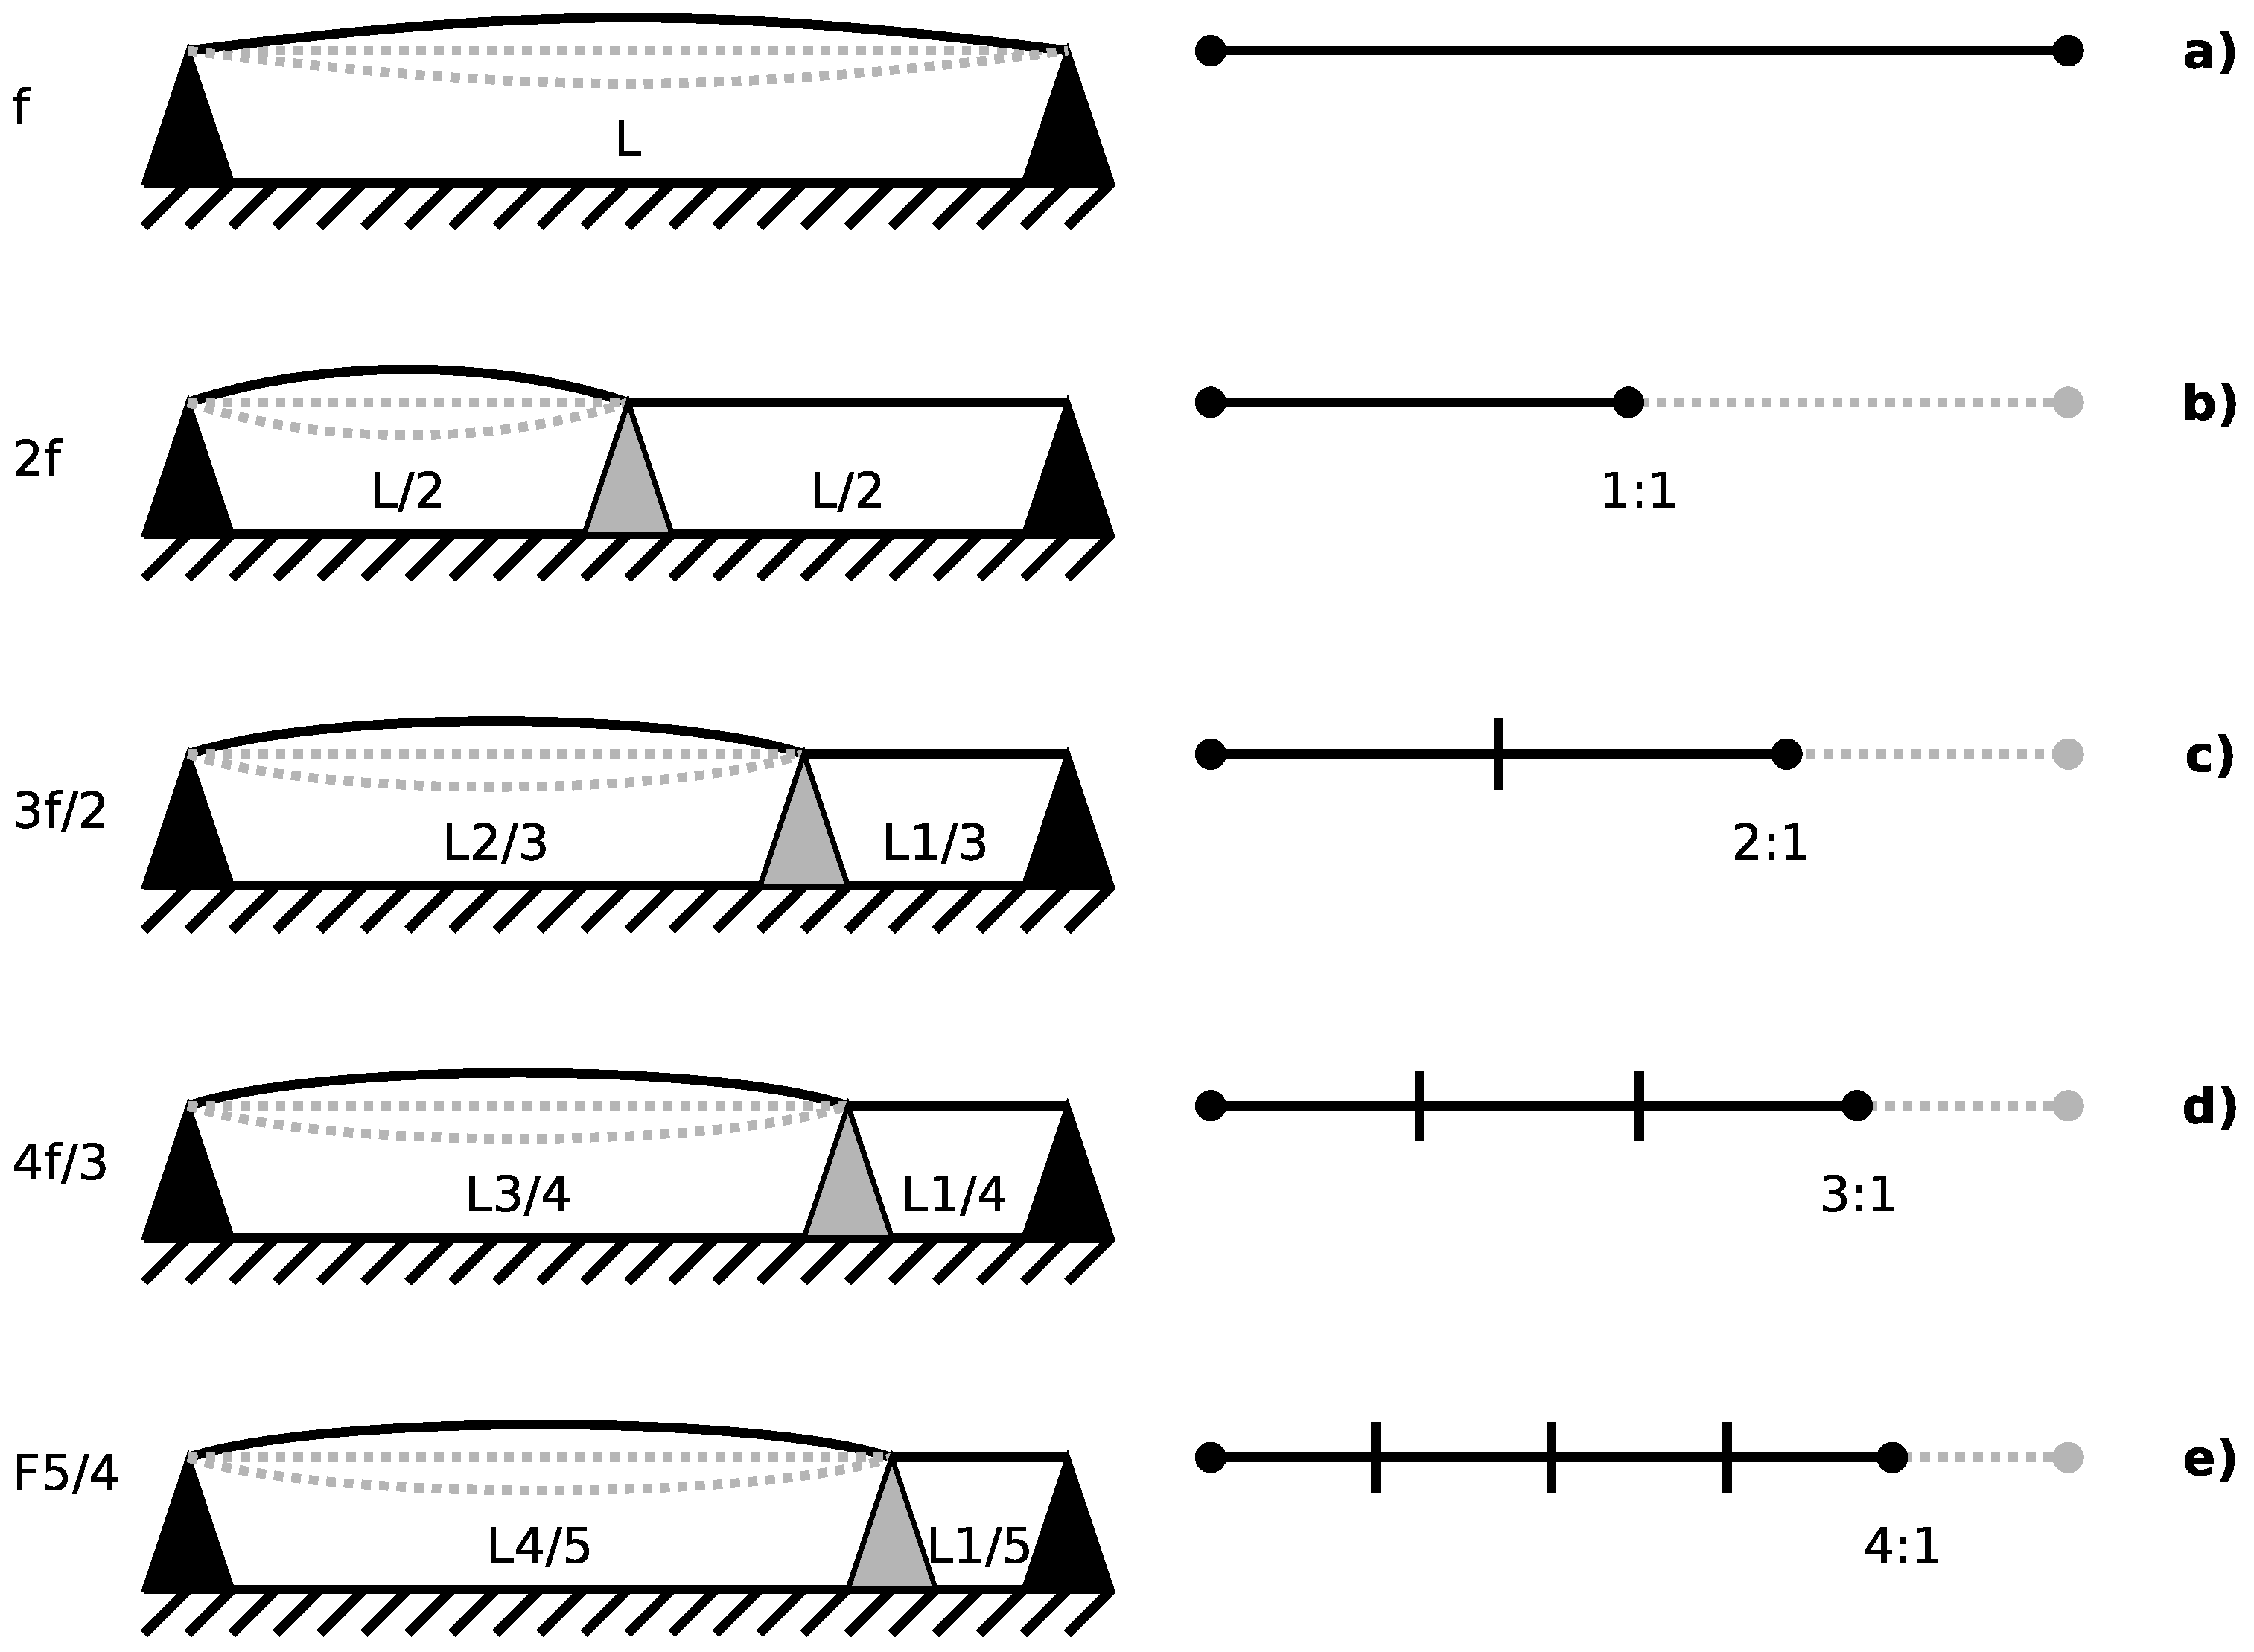
\includegraphics[width=\textwidth]{chapters/cap-musica-composer/consonancia0.eps}
\caption{Consonância entre frequências.}
\label{fig:consonancia}
\end{figure}

Quando a longitude da corda do monocórdio diminui, 
a frequência do som gerado aumenta, é dizer se obtêm tons mais agudos,
tendo longitude e frequência uma relação inversa \cite[pp. 12]{arbones2012armonia}. 
Entre os resultados obtidos com este instrumento, 
está a constatação de que algumas longitudes menores da corda, 
geravam sons mais agradáveis de ouvir, ao ser executados ao mesmo tempo com o som gerado pela corda completa \cite[pp. 12]{arbones2012armonia}.

Assim, os pitagóricos descobriram que as proporções mais simples das cordas,
eram as que geravam os sons mais agradáveis de ouvir \cite[pp. 12]{arbones2012armonia};
nas Figuras \ref{fig:consonancia}[b - e], podemos ver algumas das proporções de longitudes estudadas,
como: 1:1, 2:1, 3:1 e 4:1; que geram tons com frequências: 
$2$f, $\frac{3}{2}$f, $\frac{4}{3}$f e , $\frac{5}{4}$f.
Sendo a relação mais simples (1:1) a que provoca a duplicação da frequência (Figura \ref{fig:consonancia}b),
que na atualidade chamamos \hyperref[sec:pos:Oitava]{\textbf{oitava}}; 
a seguinte em simplicidade é a proporção 2:1 que gera um som com uma frequência de $\frac{3}{2}$f (Figura \ref{fig:consonancia}c),
que na atualidade chamamos de \textbf{intervalo de quinta};
por outro lado, nas Figuras \ref{fig:consonancia}[d-e] com frequências $\frac{4}{3}$f e , $\frac{5}{4}$f respetivamente,
a sensação de consonância diminui proporcionalmente à complexidade das frações das frequências \cite[pp. 12]{arbones2012armonia}.

Por estas observações os pitagóricos concluíram que seriam consonantes com a frequência $f$, sons com uma frequência igual a 
\begin{equation}
\label{eq:simplespita}
\frac{n+1}{n}f,
\end{equation}
sendo que o nível de consonância diminui com o aumento de ``n'' \cite[pp. 14]{arbones2012armonia}.

\PRLsep{Escala diatônica}
\label{ref:paginadiatonicanumerica}

Se usamos as frequências da Equação \ref{eq:simplespita}, para $n=\{1,2,3,4\}$,
e multiplicamos estas frequências por $\frac{3}{2}$ ou $\frac{1}{2}$, que
são as proporções de frequência que geram maior consonância,
obteremos a \hyperref[sec:pos:Diatonica]{\textbf{escala diatônica}} (E.D.).
Esta escala pode ser comparada com a \hyperref[sec:pos:Cromatica]{\textbf{escala cromática}} (E.C.)
que está \hyperref[subsec:tempigual]{\textbf{igualmente temperada}}, 
como mostra a Tabela \ref{tab:pitagorascromatica}, onde foi usada a nota musical ``dó'' como referencia, a \hyperref[sec:Tonica]{\textbf{tônica}}.
\begin{table}[h]
  \centering
  \begin{tabular}{|l|l|l|l|l|l|l|l|l|}
  \hline
  E. Diatônica  & dó & ré & mi & fá & sol & lá & si & dó \\ \hline
  \hline
  Freq. E.D.  & f  & $\frac{9}{8}$f & $\frac{5}{4}$f & $\frac{4}{3}$f & $\mathbf{\frac{3}{2}}$\textbf{f} & $\frac{5}{3}$f & $\frac{15}{8}$f & $\mathbf{2}$\textbf{f}\\ \hline
  E. Cromática & f  & $\alpha^{2}$f  & $\alpha^{4}$f  & $\alpha^{5}$f  & $\alpha^{7}$f  & $\alpha^{9}$f  & $\alpha^{11}$f  & $2$f\\ \hline \hline
  %%Error$\%$ &  0.0  & 0.23 & 0.79  & 0.11 & 0.11 & 0.91 & 0.68 & 0.0 \\ \hline
  Error$\%$ &  0.00 & 3.91 &-13.69 &-1.96 & 1.96 &-15.64&-11.73& 0.00 \\ \hline
  \end{tabular}
  \caption{Relação de frequências, usando $\alpha=2^\frac{1}{12}$.}
  \label{tab:pitagorascromatica}
\end{table}

É possível ver que existe uma ligeira diferença numérica, 
entre as proporções de frequências na escala diatônica baseada nas consonâncias descobertas pela escola pitagórica,
e as proporções de frequência de nossa atual escala cromática igualmente temperada,
no menor dos casos temos um  erro na frequência de $1.96\%$ de um \hyperref[sec:pos:Semitom]{\textbf{semitom}}, 
e no pior dos casos um erro de $15.64\%$.

\PRLsep{Análises objetivo}
Fora da subjetiva perspetiva da escola pitagórica, 
em indicar que frações mais simples na frequência geram sons consonantes; 
existem motivos objetivos para fundamentar esta afirmação.

Na Figura \ref{fig:corda32} podemos ver as sinais $y_{f}$ e $y_{\frac{3}{2}f}$, 
produzidas pelos sons com frequências $f=1000$hz e $\frac{3}{2}f$,
correspondentes a cordas de longitude $L$ e $\frac{2}{3}L$ respetivamente;
é interessante observar que se precisam \textbf{dois} ciclos completos da sinal $y_{f}$,
para que ambas sinais voltem a estar em sincronia e que a sinal soma, $y_{f}+y_{\frac{3}{2}f}$, forme um ciclo completo.


Na mesma linha de análises, na Figura \ref{fig:corda53} podemos observar as sinais $y_{f}$ e $y_{\frac{5}{3}f}$, 
produzidas pelos sons com frequências $f=1000$hz e $\frac{5}{3}f$,
correspondentes a cordas de longitude $L$ e $\frac{3}{5}L$ respetivamente;
e similarmente ao caso anterior, observamos que se precisam \textbf{três} ciclos completos da sinal $y_{f}$,
para que ambas sinais voltem a estar em sincronia e que a sinal soma, $y_{f}+y_{\frac{5}{3}f}$, forme um ciclo completo.

\begin{figure}
    \centering
    \begin{subfigure}[b]{0.8\textwidth}
        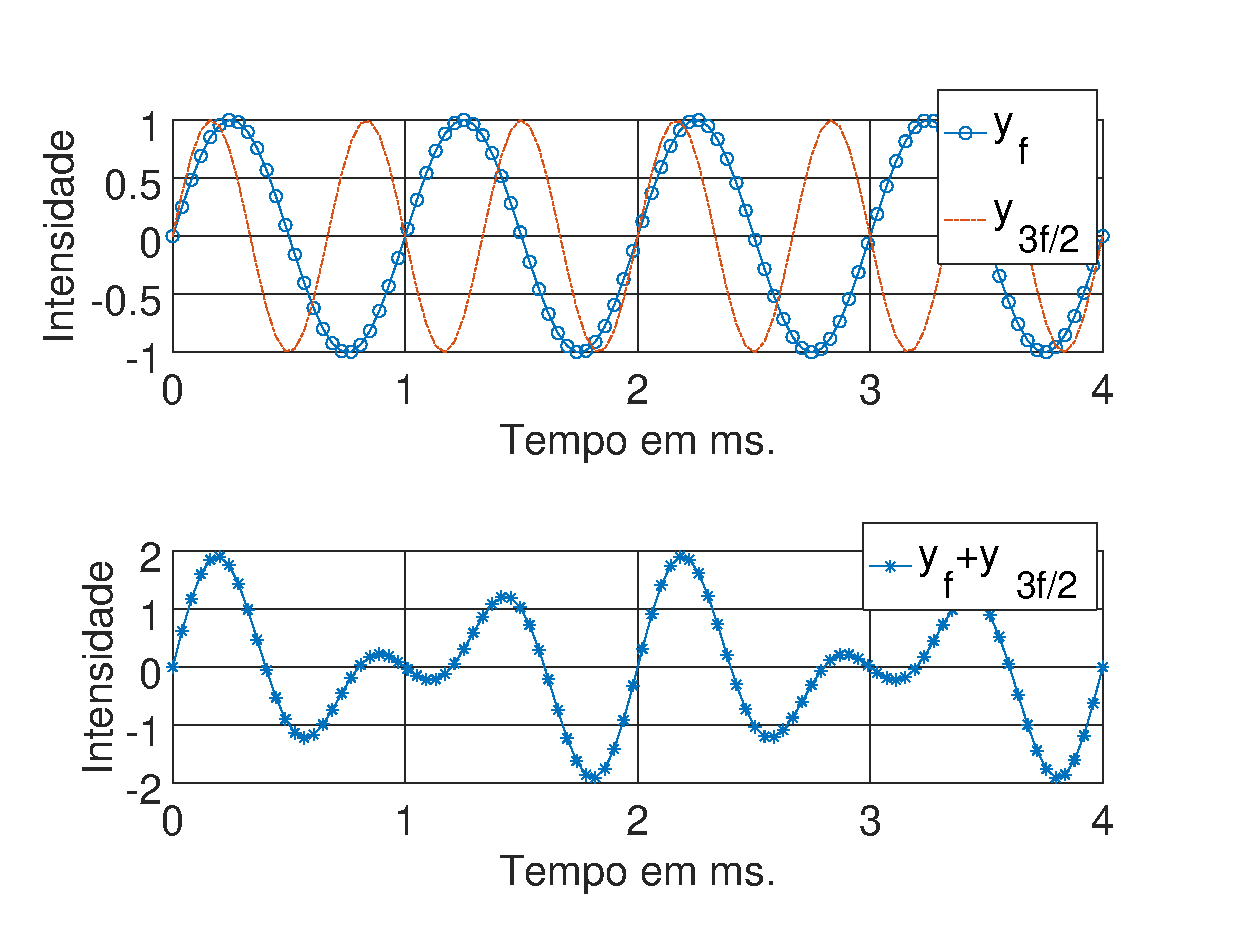
\includegraphics[width=\textwidth]{chapters/cap-musica-composer/consonancia32.eps}
        \caption{Consonância entre sinais com frequências $f$ e $\frac{3}{2}f$}
        \label{fig:corda32}
    \end{subfigure}
    ~ %add desired spacing between images, e. g. ~, \quad, \qquad, \hfill etc. 
      %(or a blank line to force the subfigure onto a new line)
    \begin{subfigure}[b]{0.8\textwidth}
        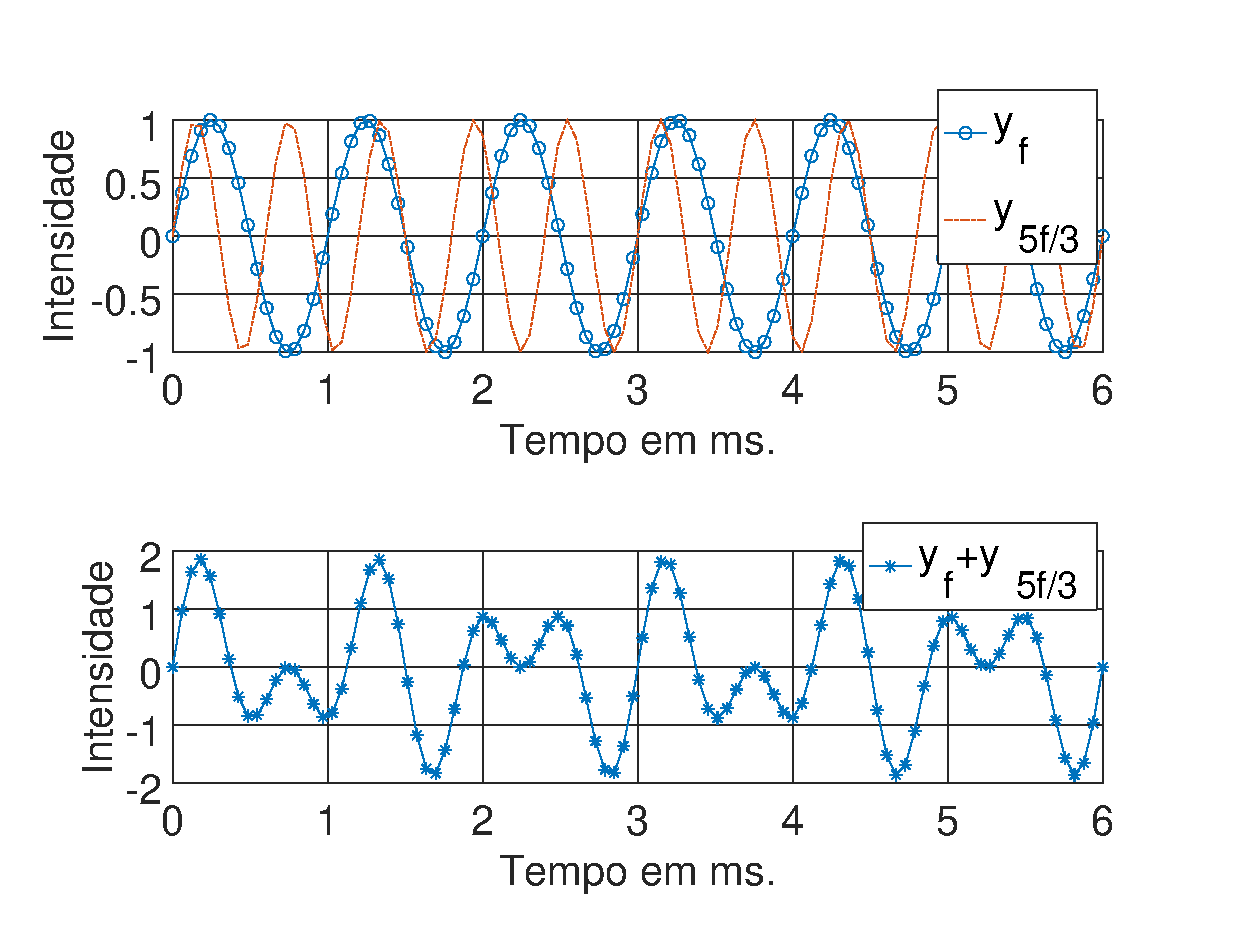
\includegraphics[width=\textwidth]{chapters/cap-musica-composer/consonancia53.eps}
        \caption{Consonância entre sinais com frequências $f$ e $\frac{5}{3}f$}
        \label{fig:corda53}
    \end{subfigure}
\caption{Analises de consonância.}
\label{fig:consonanciaper}
\end{figure}

Assim, deduzimos que pela forma fraccionaria e relativa das frequência nas sinais, 
podemos usar o denominador da fração na frequência,
para conhecer quantos ciclos debem passar para que a ambas sinais em estudo voltem a estar em sincronia;
de modo que seremos capazes de relacionar um estado de maior nível de dissonância (N.D.) com um maior número de ciclos.
A Tabela \ref{tab:pitagorascromatica2} mostra estas relações, 
porém foram agregadas as letras ``a'' e ``b'' para indicar menor e maior dissonância respetivamente,
nos casos com igual N.D., este critério foi aplicado tomando em conta que a escala
que comumente temos num piano está igualmente temperada,
é como vimos na Tabela  \ref{tab:pitagorascromatica},
existe um erro de aproximação a estas frações;
de modo que foi colocada a etiqueta de ``b'' ao caso de maior erro e a etiqueta de ``a'' ao de menor.
\begin{table}[h]
  \centering
  \begin{tabular}{|l|l|l|l|l|l|l|l|l|}
  \hline
  E. Diatônica    & dó & ré & mi & fá & sol & lá & si & dó \\ \hline
  \hline
  Semitons E.C.   & 0  & 2  & 4  & 5  & 7  & 9  & 11 & 12 \\ \hline
  Freq. E.D.  & f  & $\frac{9}{8}$f & $\frac{5}{4}$f & $\frac{4}{3}$f & $\mathbf{\frac{3}{2}}$\textbf{f} & $\frac{5}{3}$f & $\frac{15}{8}$f & $\mathbf{2}$\textbf{f}\\ \hline \hline
  N.D. &  0 & 8a & 4 & 3a & 2 & 3b & 8b & 1 \\ \hline
  \end{tabular}
  \caption{Nível de dissonância com a nota musical dó.}
  \label{tab:pitagorascromatica2}
\end{table}

\begin{example}
Com a ajuda de um piano, que esteja igualmente temperado,
use a nota dó como referencia e comprove o nível de consonância com todas as demais notas musicais;
verifique se concorda com o mostrado na Tabela \ref{tab:pitagorascromatica2}.
\end{example}~

\PRLsep{Conclusões}

Finalmente, podemos concluir que existe uma maior consonância entre
\begin{itemize} 
\item os tons com frequências $f$ e $2f$, e 
\item os tons com frequências $f$ e $\frac{3}{2}f$;
\end{itemize}
para outros valores de frequência, 
como entre $f$ e $\frac{4}{3}f$, o nível de consonância diminui  
 gradualmente com o aumento da complexidade das frações nas frequências.

Na música atual, as relações de consonância são usadas na escala cromática, 
em notas musicais com:
\begin{itemize} 
\item Uma oitava de diferença, para as frequências relacionadas como $f$ e $2f$, 
por exemplo: dó e dó'.
\item Um intervalo de quinta, sete semitons, para frequências relacionadas como  $f$ e $\frac{3}{2}f$, 
por exemplo: dó e sol. Porém, numa escala igualmente temperada, 
os 7 semitons são uma aproximação\footnote{Sim, você está supondo certo,
toda a música atual está ligeiramente ``desafina'', pois usa uma aproximação para a consonância.}
 da fração $\frac{3}{2}$.
\end{itemize}~


Os seres humanos não nos sentimos confortáveis ao terminar o dia com um argumento não resolvido; 
da mesma forma, não apreciamos terminar nossa música com uma dissonância não resolvida \cite[pp. 26]{wright2012essential}.

 

\section{Música tonal, modal e atonal}
\label{sec:ModosEntenderMusica}
Podem existir vários modos de entender a música, como por exemplo o ``tonal'' e o ``modal''.
A diferencia entre estes dois paradigmas da música, 
radica na forma em que a música desenvolve sua existência no tempo \cite[pp. 155]{arbones2012armonia}.


\subsection{Música tonal}
\label{sec:MusicaTonal}
\index{Música!Música tonal}
A música tonal inicia no Barroco, aproximadamente entre os anos 1600 e 1750,
e tem a  caraterística de ser um tipo de  música que se projeta para adiante;
em cada momento da musica tonal, um acorde pelo geral conduz a outro,
pois existe um jogo de tensão e relaxação que deve ser resolvido,
a este rol dos acordes chama-se ``função de acorde'' \cite[pp. 155-156]{arbones2012armonia}.


Na música tonal, 
as notas musicais são organizadas seguindo a importância destas ao redor de uma nota  principal,
que foi batizada como ``tônica'', ou centro tonal \cite[pp. 27]{arbones2012armonia}.
Este ordem segue as regras de \hyperref[ref:paginadiatonicanumerica]{\textbf{consonância}} observadas pela escola pitagórica,
que provoca que as alturas dos tons na \hyperref[sec:pos:Diatonica]{\textbf{escala diatônica}} 
estejam formados usando frações em função de uma frequência fundamental, a tônica.

Mesmo que a disposição fracionaria das notas na música tonal, gere melodias muito consonantes,
problemas\footnote{Problemas na diminuição da consonância; é dizer o aumento da dissonância.} 
podem ser encontrados sim se desenvolvem melodias ao redor de uma nota diferente da tônica;
e dizer, longe da nota musical da qual foram calculadas as demais notas \cite[pp. 28]{arbones2012armonia},
de ali a importância da tônica na música tonal.

\subsubsection{Música tonal desde seculo XX}
A maioria das músicas  escritas desde o seculo XX é diatônica e tonal;
porém, atualmente a música tonal não tem mais a mesma velha definição de tonalidade dos seculos anteriores  \cite[pp. 63]{copland1974ouvir},
em primeiro lugar porque a música atual, geralmente usa instrumentos com \hyperref[subsec:tempigual]{\textbf{temperamento igual}},
o que provoca que não exista uma nota mais importante que as demais, 
pelo que transposições podem ser feitas sem alterar a consonância de uma peça musical.
Outra consequência do \hyperref[subsec:tempigual]{\textbf{temperamento igual}},
é que a o intervalo de quinta considerado antes como de uma consonância perfeita,
com frequências que tem uma proporção 3/2 (1.5), é agora medido com sete semitons (aproximadamente 1.49830707687668),
obtendo desta maneira só uma aproximação à consonância.\\




\subsection{Música modal}
\label{sec:MusicaModal}
\index{Música!Música modal}

No estilo modal o tempo tem se interpretado de dois jeitos diferentes:
\begin{itemize}
\item Como uma eternidade; como por exemplo no canto gregoriano; e dizer 
sem noção de passado, presente ou futuro.
\item Com o tempo como presente continuo, 
o acontecimento sonoro é completo em cada instante; é dizer,
 o sonido atual não esta condicionado ao passado ou ao futuro;
como por exemplo o ``bebop jazz''\cite[pp. 156]{arbones2012armonia}.
\end{itemize}



\subsection{Música atonal: dodecafonismo}
\label{sec:MusicaAtonal}
\index{Música!Música atonal}
O dodecafonismo é uma técnica de composição musical, 
criada na década de 1920 pelo compositor austríaco Arnold Schonberg \cite[pp. 121]{arbones2012armonia}\cite[pp. 263]{holst1998abc}.


A técnica dodecafônica, ou com igualitarismo tonal,
procura a ideia de uma música \textbf{atonal}; é dizer carente de centro tonal,
que se desliga de uma maior gravitação a uma nota, a tônica, sobre as demais;
O dodecafonismo desenvolve um método para evitar a preponderância de uma nota sobre outras,
de modo que todas tem o mesmo valor relativo,
e possam ser apreciadas da mesma forma numa composição musical 
\cite[pp. 122]{arbones2012armonia}.

Para evitar a centralização da peça musical numa nota especifica,
o compositor deve completar ciclos que usem as 12 notas 
(brancas e negras numa oitava nu piano). 
Apos uma nota musical ser usada, 
esta não podia volver a ser usada ate o seguinte ciclo de 12 notas \cite[pp. 123]{arbones2012armonia}.


 
\section{Tônica e dominante}
\index{Música!Tônica}


\subsection{Tônica}
\label{sec:Tonica}
Na \hyperref[sec:MusicaTonal]{\textbf{música tonal}} toda melodia tem uma ``tônica''; 
é dizer, uma nota mais importante \cite[pp. 19]{holst1998abc}, 
pois como é explicado na Seção \ref{sec:consonancia}, se temos uma escala diatônica,
onde as notas são afinadas buscando a \hyperref[ref:consonancia]{\textbf{consonância}},
como foi indicada pela escola pitagórica; então todas as notas são expressadas,
como uma fração de uma nota principal, a tônica. 
Como uma consequência inesperada, deste tipo de afinação, 
qualquer transposição de uma melodia, longe deste centro tonal, 
provocará a introdução de dissonâncias,
a este problema chama-se a ``coma pitagórica'' \cite[pp. 24]{arbones2012armonia}.
 

Do mesmo modo que o sujeito numa oração é identificável, a tônica também é identificável;
no âmbito literário o uso das palavras numa frase, 
provoca que identifiquemos entre elas ao sujeito, pelo papel que esta cumpre na frase.
Acontece da mesma forma na linguagem musical; numa melodia,
a ordem da escolha consecutiva das notas musicais, 
fazem que a tônica seja perceptível, pois dá à melodia ou harmonia, 
seu sentido musical como o centro a onde se converge para dar sentido de finalização a frase \cite[pp. 19]{holst1998abc}.

Assim a tônica é identificável, numa melodia ou harmonia, 
porque esta é geralmente  usada no final  da frase musical, 
quando se quer dar uma sensação de um final forte;
é dizer que expressa claramente a conclusão de uma ideia.
Nesse caso, a tônica comumente é usado apos uma nota que está separada um 
\hyperref[sec:intervalomelodico]{\textbf{intervalo}} de quinta;
chama-se a está nota de \hyperref[sec:dominante]{\textbf{dominante}}.

\subsection{Dominante}
\label{sec:dominante}

O intervalo entre a tônica e a quinta nota musical mais aguda 
(\hyperref[fig:abc-iquinta2]{\textbf{intervalo de quinta}} ascendente), 
na escala diatônica, 
é o intervalo mais importante\footnote{Expeto se a tônica é um si, nesse caso é melhor contar 7 semitons},
pois é o intervalo \hyperref[tab:pitagorascromatica2]{\textbf{mais consonante}}, 
só superado pelo intervalo de oitava. 
Por conta disto o quinto grau dos modos da escala diatônica é chamado  de ``dominante'';
tendo esta uma forte atração com a tônica. 
Esta caraterística é um dos componentes que ajudam a manter interessante  uma melodia \cite[pp. 24]{holst1998abc}.
Na Seção \ref{sec:Cadencia}, onde é tratado o tema da \hyperref[sec:Cadencia]{\textbf{cadência}},
pode ser encontrada mais informação sobre a relação entre a tônica e a dominante.

\subsection{A tônica e as escalas modais}
Qualquer nota da escala diatônica podem ser escolhidas como tônica;
assim, existira para cada uma destas escolhas existirá um distinto grupo de sete notas,
ordenadas em relação a esta tônica. Estos grupos são chamados modos \cite[pp. 21]{holst1998abc};
a Tabela \ref{tab:modosdiatonica}, mostra o nome de todos os modos possíveis da escala diatônica,
e indica com números romanos todos os intervalos possíveis,
de modo que ``I'' indica a tônica, e ``IV'' indica a dominante.

\begin{table}[h]
  \centering
  \begin{tabular}{|l||l|l|l|l|l|l|l|}
  \hline
  Modo      & I   & II  & III & IV  & V   & VI  & VII \\ \hline \hline
  Jônico    & dó  & ré  & mi  & fá  & sol & lá  & si  \\ \hline
  Dórico    & ré  & mi  & fá  & sol & lá  & si  & dó  \\ \hline
  Frígio    & mi  & fá  & sol & lá  & si  & dó  & ré  \\ \hline
  Lídio     & fá  & sol & lá  & si  & dó  & ré  & mi  \\ \hline
  Mixolídio & sol & lá  & si  & dó  & ré  & mi  & fá  \\ \hline
  Eólica    & lá  & si  & dó  & ré  & mi  & fá  & sol \\ \hline
  Lócrio    & si  & dó  & ré  & mi  & fá  & sol & lá  \\ \hline
  \end{tabular}
  \caption{Escalas modais e os graus.}
  \label{tab:modosdiatonica}
\end{table}

\subsection{Nome dos graus na escala diatônica}
A escala diatônica está formada por oito graus, 
sendo que cada um destes tem uma função especifica \cite[pp. 31]{cardoso1973curso};
A Tabela \ref{tab:relacaotonica} mostra todos os nomes para estes graus, 
o grau VIII não foi colocado pois é a repetição do grau I. 
\begin{table}[h]
  \centering
  \begin{tabular}{|l|l|p{7cm}|}
  \hline
  Nome           & Grau & Função\\ \hline \hline
  Tônica         & I    & Repouso natural da tonalidade.\\ \hline
  Supertônica    & II   & Grau acima da tônica.\\ \hline 
  Mediante       & III  & Grau intermediário entre a tônica e a dominante.\\ \hline 
  Subdominante   & IV   & Grau abaixo da dominante.\\ \hline 
  Dominante      & V    & Quinto grau a partir da tônica.\\ \hline 
  Superdominante & VI   & Grau acima da dominante.\\ \hline 
  Sensível       & VII  & Sétimo grau acima da tônica. \\ \hline
  \end{tabular}
  \caption{Nome dos graus nas notas musicais.}
  \label{tab:relacaotonica}
\end{table}


%%%%%%%%%%%%%%%%%%%%%%%%%%%%%%%%%%%%%%%%%%%%%%%%%%%%%%%%%%%%%%%%%%%%%%%%%%%%%%%%
%https://pt.wikipedia.org/wiki/T%C3%B4nica
 
%%%%%%%%%%%%%%%%%%%%%%%%%%%%%%%%%%%%%%%%%%%%%%%%%%%%%%%%%%%%%%%%%%%%%%%%%%%%%%%%
\section{Cadência}
\label{sec:Cadencia}
\index{Música!Cadência}

\begin{tcbinformation}{Música cadenciosa}
\index{Música!Música cadenciosa}
\label{ref:musicacadenciosa}
É aquela que tem um ritmo facilmente apreciável, na qual as terminações, ou seja cadências,
são fáceis de perceber \cite[pp. 60]{pedrell2009diccionario}.
Para que uma música seja cadenciada é preciso que ritmo e harmonia se combinem  
para dar uma sensação de exatidão \cite[pp. 68]{melcior1859diccionario}.
\end{tcbinformation} 


O final da frase musical está marcado pela cadência, 
este nome vem da palavra ``cadenza''  em italiano que significa caindo ou cessando \cite[pp. 34]{bennett1993elementos} \cite[pp. 68]{melcior1859diccionario}. 
As cadências existem nas frases melódicas ou harmônicas, 
e são identificáveis como os períodos de repouso entre as frases musicais;
estas cumprem o mesmo papel que os signos de pontuação na gramática, 
já seja como virgulas, pontos e virgulas, pontos, signos de interrogação
\cite[pp. 66,67]{melcior1859diccionario} \cite[pp. 34]{bennett1993elementos}, 
etc.


%%%%%%%%%%%%%%%%%%%%%%%%%%%%%%%%%%%%%%%%%%%%%%%%%%%%%%%%%%%%%%%%%%%%%%%%%%%%%%%%
\subsection{Cadência harmônica}
\label{sec:CadenciaHarmonica}
\index{Música!Cadência harmônica}

As cadencias harmônicas estão representadas por um par de ``acordes''
que são usados para finalizar uma frase musical, estas tem um sentido de mensagem. 

Entre os tipos de cadencias harmônicas, 
temos as que nos dão a liberdade expressar uma pausa momentânea, suspenso ou o final de uma ideia.

A Tabela \ref{tab:tiposdecadencia} mostra algumas desta opções, 
na primeira coluna temos os nomes dos tipos de cadencias,
na segunda coluna temos a ordem e os graus dos acordes que são usados para gerar essa cadência 
e na terceira coluna está a descrição de cada um dos tipos de cadência.

\begin{table}[h]
  \centering
  \begin{tabular}{|p{4cm}|l|p{8cm}|}
  \hline
  Nome & Acordes   & Analogia \\ \hline
  \hline
  Cadência perfeita & V-I       & Dá sentido de algo perfeitamente acabado, 
  equivalente a um ponto final na gramática \cite[pp. 34]{bennett1993elementos}. \\ \hline
  
  Cadência plagal   & IV-I      & Dá um sentido equivalente a um ponto final na gramática, 
  também é chamado de cadência do ``Amém'' 
  por seu uso em hinos religiosos \cite[pp. 34]{bennett1993elementos} \\ \hline

  Cadência imperfeita ou semicadência \cite[pp. 103]{grabner2001teoria} & ?-V    & Acontece quando se vá de um grau qualquer para finalizar na dominante (V), 
  porém é comum ver que se usam:
  I-V,II-V e IV-V. Esta cadência dá à música a sensação de um final incompleto, 
  seu efeito é similar ao de uma virgula na gramática,
  \cite[pp. 34]{bennett1993elementos}. \\ \hline

  Cadência interrompida & V-($\neq$I) & Acontece quando se sugere que acontecerá uma cadencia V-I (dominante-tônica),
  porém apos V se finaliza em qualquer grau 
  diferente da \hyperref[sec:Tonica]{\textbf{tônica}}, geralmente VI,
  e dá uma sensação de surpresa e de interrupção à música; ou seja uma frase incompleta.
  \cite[pp. 35]{bennett1993elementos}. \\ \hline  
\end{tabular}
  \caption{Tipos de cadência harmônica.}
  \label{tab:tiposdecadencia}
\end{table}

\begin{example}
A Figura \ref{fig:abc-perfeita1} mostra uma cadência perfeita para uma tônica em acorde de dó.
A cadência dá a sensação de uma frase com ponto final.
\end{example}

\begin{figure}[H]
\centering
\begin{abc}[name=abc-perfeita1,width=1.0\linewidth]
X: 1 % start of header
K: C % scale: C major
M: 2/4 %meter - compasso
V:1 %name="Pauta com clave de fá"   sname="Pauta com clave de fá"
[V:1] | [C2 E2 G2] [F2 A2 C'2]| [E2 G2 B2] [G2 B2 D'2]| [F2 A2 C'2] [G2 B2 D'2]| [C2 E2 G2] z2|
w: ~ ~ ~ ~ ~ V I
\end{abc}
\caption{Cadência perfeita.}
\label{fig:abc-perfeita1}
\end{figure}

\begin{example}
A Figura \ref{fig:abc-plagal1} mostra uma cadência plagal para uma tônica em acorde de dó.
A cadência dá a sensação de uma frase com ponto ao  final.
\end{example}

\begin{figure}[H]
\centering
\begin{abc}[name=abc-plagal1,width=1.0\linewidth]
X: 1 % start of header
K: C % scale: C major
M: 2/4 %meter - compasso
V:1 %name="Pauta com clave de fá"   sname="Pauta com clave de fá"
%[V:1] | [E2 G2 B2] [F2 A2 C'2]| [E2 G2 B2] [G2 B2 D'2]| [C2 E2 G2] z2|
[V:1] | [C2 E2 G2] [F2 A2 C'2]| [E2 G2 B2] [G2 B2 D'2]| [E2 G2 B2] [F2 A2 C'2]| [C2 E2 G2] z2|
w: ~ ~ ~ ~ ~ IV I
\end{abc}
\caption{Cadência plagal.}
\label{fig:abc-plagal1}
\end{figure}

\begin{example}
A Figura \ref{fig:abc-imperfeita1} mostra uma cadência imperfeita para uma tônica em acorde de dó.
A cadência dá a sensação de uma frase com um final débil, como de uma mistura de signo de admiração e interrogação.
\end{example}

\begin{figure}[H]
\centering
\begin{abc}[name=abc-imperfeita1,width=1.0\linewidth]
X: 1 % start of header
K: C % scale: C major
M: 2/4 %meter - compasso
V:1 %name="Pauta com clave de fá"   sname="Pauta com clave de fá"
[V:1] | [C2 E2 G2] [F2 A2 C'2]| [E2 G2 B2] [G2 B2 D'2]| [E2 G2 B2] [F2 A2 C'2]| [G2 B2 D'2] z2|
w: ~ ~ ~ ~ ~ IV V
\end{abc}
\caption{Cadência imperfeita.}
\label{fig:abc-imperfeita1}
\end{figure}


\begin{example}
A Figura \ref{fig:abc-interrompida1} mostra uma cadência interrompida para uma tônica em acorde de dó.
A cadência dá a sensação de uma frase incompleta.
\end{example}

\begin{figure}[H]
\centering
\begin{abc}[name=abc-interrompida1,width=1.0\linewidth]
X: 1 % start of header
K: C % scale: C major
M: 2/4 %meter - compasso
V:1 %name="Pauta com clave de fá"   sname="Pauta com clave de fá"
[V:1] | [C2 E2 G2] [F2 A2 C'2]| [E2 G2 B2] [G2 B2 D'2]| [E2 G2 B2] [G2 B2 D'2]| [A2 C'2 E'2] z2|
w: ~ ~ ~ ~ ~ V VI
\end{abc}
\caption{Cadência interrompida.}
\label{fig:abc-interrompida1}
\end{figure}

%%%%%%%%%%%%%%%%%%%%%%%%%%%%%%%%%%%%%%%%%%%%%%%%%%%%%%%%%%%%%%%%%%%%%%%%%%%%%%%%
\subsection{Cadência melódica} 
\label{subsec:cadenciamelodica}
Quando nos referimos à forma em que uma melodia é finalizada,
estamos falando da cadencia melódica; esta pode ser categorizada em: 
\begin{itemize}
\item \textbf{Cadências}, se o repouso é equivalente a um ponto na gramática \cite[pp. 66,67]{melcior1859diccionario},
como o produzido por uma dominante (V) seguida de um tônica (I).
\item \textbf{Semicadências}, se repouso é equivalente a um ponto e virgula na gramática \cite[pp. 66,67]{melcior1859diccionario};
esta também é chamada de cadencia imperfeita e se carateriza por terminar numa dominante (V) 
que geralmente vem precedida por  I, II ou IV \cite[pp. 103]{grabner2001teoria}; 
é possível ver este tipo de cadencia no final da frase antecedente de um 
\hyperref[sec:Periodo]{\textbf{período}} \cite[pp. 21]{latham2008diccionario}.
\item \textbf{Quartos de cadência}, se o repouso é igual a uma virgula \cite[pp. 66,67]{melcior1859diccionario}.
\end{itemize}~

Todas estas cadencias dão à melodia uma sensação da conclusão de uma ideia; 
porém, cada uma destas nos deixa uma perspetiva diferente sobre o que vem depois e quando.

Além dos tipos de cadencias melódicas anteriormente mencionadas, podemos achar também a:
\begin{itemize}
\item \textbf{Cadência interrompida}, este tipo de cadencia se verifica 
quando ao final de um período sugerimos que iremos de 
\hyperref[sec:dominante]{\textbf{dominante}} a \hyperref[sec:Tonica]{\textbf{tônica}},
porém terminamos em qualquer outro grau; ou seja pulamos da dominante a um grau diferente da tônica 
\cite[pp. 67]{melcior1859diccionario} \cite[pp. 60]{pedrell2009diccionario}. 
\end{itemize}~

Em geral veremos um uso aprimorado das cadências, na frase consequente de um \hyperref[sec:Periodo]{\textbf{período}},
onde o tipo do cadência ajudará a expressar o uso que esta terá na peça musical  \cite[pp. 66,67]{melcior1859diccionario}.

\begin{example}
A Figura \ref{fig:abc-frasemelodica1} mostra duas frases com tônica em dó, 
a primeira frase com uma semicadencia (VI-V) e a segunda frase com uma cadência (V-I).
\end{example}

\begin{figure}[H]
\centering
    \includegraphics[width=\textwidth]{chapters/cap-musica-composer/frasemelodica1-1.eps}
\caption{Duas frases melódicas com tônica em dó.}
\label{fig:abc-frasemelodica1}
\end{figure}

\begin{example}
A Figura \ref{fig:abc-frasemelodica2} mostra duas frases  com tônica em sol, 
a primeira frase com uma cadência interrompida (V-III) e a segunda frase com uma cadência (V-I).
\end{example}

\begin{figure}[H]
\centering
    \includegraphics[width=\textwidth]{chapters/cap-musica-composer/frasemelodica2-1.eps}
\caption{Duas frases melódicas com tônica em sol.}
\label{fig:abc-frasemelodica2}
\end{figure}
% https://es.wikipedia.org/wiki/Cadencia_(música)

% https://en.wikipedia.org/wiki/Cadence



%%%%%%%%%%%%%%%%%%%%%%%%%%%%%%%%%%%%%%%%%%%%%%%%%%%%%%%%%%%%%%%%%%%%%%%%%%%%%%%%
\section{Articulação}
\label{sub:Articulação}
\index{Música!Articulação}

Nas partituras podemos ver alguns símbolos, 
que o compositor coloca como indicação ao interprete,
para informar como as notas musicais devem ser executadas ou 
articuladas entre sim \cite[pp. 56]{alves2004teoria}.
%%%%%%%%%%%%%%%%%%%%%%%%%%%%%%%%%%%%%%%%%%%%%%%%%%%%%%%%%%%%%%%%%%%%%%%%%%%%%%%%
\subsection{Legato ou ligadura de expressão}
\label{subsec:Legato}
\index{Música!Legato}
O  ``legato'' é um símbolo  que indica uma ligadura de expressão entre as notas,
neste caso a informação que da o compositor é que as
notas devem ser executadas sem interrupções,
criando uma mudança de tons gradual para passar de uma nota musical a outra \cite[pp. 56]{alves2004teoria}.

\begin{example}
A Figura \ref{fig:legato1} mostra um exemplo de uso do legato. 
Alguns instrumentos podem facilmente articular um legato, por exemplo o violino.
\end{example}

\begin{figure}[h!]
\centering
\begin{abc}[name=abc-legato1,width=0.80\linewidth]
X: 1 % start of header
K: C % scale: C major
M: 2/4 %meter - compasso
 (G2 E2 | G1  A1  G1 E1 )|
\end{abc}
\caption{Melodia com notas que devem ser executadas de forma ligada.}
\label{fig:legato1}
\end{figure}

%%%%%%%%%%%%%%%%%%%%%%%%%%%%%%%%%%%%%%%%%%%%%%%%%%%%%%%%%%%%%%%%%%%%%%%%%%%%%%%%
\subsection{Staccato}
\label{subsec:Staccato}
\index{Música!Staccato}

O staccato é um símbolo, desenhado com um ponto (.), 
que indica a diminuição na \hyperref[sec:pos:Duracion]{\textbf{duração}} de uma nota (aproximadamente um 50\%), 
dando nela um efeito de separação ou destaque \cite[pp. 56]{alves2004teoria}.

\begin{example}
A Figura \ref{fig:staccato1a} mostra um exemplo de uso do staccato. 
Na Figura \ref{fig:staccato1b} podemos ver uma escrita equivalente, sem o uso do símbolo de staccato.
\end{example}

\begin{figure}[h!]
\centering
\begin{subfigure}[c]{0.80\textwidth}
\begin{abc}[name=abc-staccato1a]
X: 1 % start of header
K: C % scale: C major
M: 2/4 %meter - compasso
 .G2 .E2 | .G1  .A1  .G1 .E1 | 
\end{abc}
\caption{Notação de notas musicais em staccato.}
\label{fig:staccato1a}
\end{subfigure}
~ %
\begin{subfigure}[c]{1.00\textwidth}
\begin{abc}[name=abc-staccato1b]
X: 1 % start of header
K: C % scale: C major
M: 2/4 %meter - compasso
 G1 z1 E1 z1 | G1/2 z1/2 A1/2 z1/2 G1/2 z1/2 E1/2 z1/2 | 
\end{abc}
\caption{Forma de execução de notas musicais em staccato.}
\label{fig:staccato1b}
\end{subfigure}
\caption{Melodia com notas que devem ser executadas em staccato.}
\label{fig:staccato1}
\end{figure}

\subsubsection{Staccatissimo}

O staccatissimo, staccato seco ou martelado é um símbolo, com uma função similar ao staccato;
porem indica uma diminuição maior na \hyperref[sec:pos:Duracion]{\textbf{duração}} de nota (aproximadamente ao 25\%) \cite[pp. 56]{alves2004teoria}.

\begin{example}
A Figura \ref{fig:staccatissimo1a} mostra um exemplo de uso do staccatissimo. 
Na Figura \ref{fig:staccatissimo1b} podemos ver uma escrita equivalente, sem o uso do símbolo de staccatissimo.
\end{example}

\begin{figure}[h!]
\centering
\begin{subfigure}[c]{0.80\textwidth}
\begin{abc}[name=abc-staccatissimo1a]
X: 1 % start of header
K: C % scale: C major
M: 2/4 %meter - compasso
 !wedge!G2 !wedge!E2 | !wedge!G1  !wedge!A1  !wedge!G1 !wedge!E1 | 
\end{abc}
\caption{Notação de notas musicais em staccatissimo.}
\label{fig:staccatissimo1a}
\end{subfigure}
~ %
\begin{subfigure}[c]{1.00\textwidth}
\begin{abc}[name=abc-staccatissimo1b]
X: 1 % start of header
K: C % scale: C major
M: 2/4 %meter - compasso
 G1/2 z3/2 E1/2 z3/2 | G1/4 z3/4 A1/4 z3/4 G1/4 z3/4 E1/4 z3/4 | 
\end{abc}
\caption{Forma de execução de notas musicais em staccatissimo.}
\label{fig:staccatissimo1b}
\end{subfigure}
\caption{Melodia com notas que devem ser executadas em staccato.}
\label{fig:staccatissimo1}
\end{figure}

%%%%%%%%%%%%%%%%%%%%%%%%%%%%%%%%%%%%%%%%%%%%%%%%%%%%%%%%%%%%%%%%%%%%%%%%%%%%%%%%
\subsection{Tenuto ou sostenuto}
\label{subsec:Tenuto}
\index{Música!Tenuto}

O tenuto é um símbolo, desenhado com uma linha reta (-), 
que indica que deve ser sustentada a 
\hyperref[sec:pos:Duracion]{\textbf{duração}} e a \hyperref[sec:pos:Intensidade]{\textbf{intensidade}} da nota ao máximo \cite[pp. 56]{alves2004teoria}.

\begin{example}
A Figura \ref{fig:tenuto1} mostra um exemplo de uso do tenuto. 
\end{example}


\begin{figure}[h!]
\centering
\begin{abc}[name=abc-tenuto1,width=0.80\linewidth]
X: 1 % start of header
K: C % scale: C major
M: 2/4 %meter - compasso
 !tenuto!G2 !tenuto!E2 | !tenuto!G1  !tenuto!A1  !tenuto!G1 !tenuto!E1 |
\end{abc}
\caption{Melodia com notas que devem ser executadas de forma sustenido.}
\label{fig:tenuto1}
\end{figure}

%%%%%%%%%%%%%%%%%%%%%%%%%%%%%%%%%%%%%%%%%%%%%%%%%%%%%%%%%%%%%%%%%%%%%%%%%%%%%%%%
\subsection{Accénto}
\label{subsec:Accento}
\index{Música!Accénto}

O accénto é um símbolo, desenhado com  (>), 
que indica que a nota deve ser acentuada; 
é dizer, esta deve receber um aumento de \hyperref[sec:pos:Intensidade]{\textbf{intensidade}} \cite[pp. 56]{alves2004teoria}.

\begin{example}
A Figura \ref{fig:accento1} mostra um exemplo de uso do accénto.
Onde os tempos fracos tem um aumento de intensidade provocando \hyperref[sec:contratempo]{\textbf{contratempos}}. 
\end{example}


\begin{figure}[h!]
\centering
\begin{abc}[name=abc-accento1,width=0.80\linewidth]
X: 1 % start of header
K: C % scale: C major
M: 2/4 %meter - compasso
 G2 !>!E2 | G1  !>!A1  !>!G1 !>!E1 |
\end{abc}
\caption{Melodia com notas que devem ser executadas de forma sostenida.}
\label{fig:accento1}
\end{figure}
 
\section{Recursos rítmico-melódicos}
\begin{tcbinformation}{Ideia musical}
\index{Música!Ideia musical}
\label{ref:ideiamusical}
É uma melodia pequena e muito simples  que não contem recheio né redundâncias obvias \cite[pp. 12]{howard1991aprendendo},
uma ideia pode virar facilmente num \hyperref[sec:Motivo]{\textbf{motivo}} ou uma \hyperref[sec:Frase]{\textbf{frase}} 
se esta cumpre com as suas respetivas definições.
\end{tcbinformation} 

Existem vários recursos rítmicos e melódicos aplicáveis sobre uma ideia musical
que lhe proporcionam maior interesse e a apresentam de novas formas.
Nas seguintes subseções serão apresentados alguns dos recursos mais comuns,
com este fim é usada como origem a ideia musical mostrada na Figura \ref{ritmo:ideiamusical1}. 
\begin{figure}[H]
\centering
\begin{abc}[name=abc-ideiamusical1,width=0.8\linewidth,options={-O= -c -s 1.5}]
X: 1 % start of header
K: C % scale: C major
M: 2/4 %meter - compasso
V:1 %name="Pauta com clave de fá"   sname="Pauta com clave de fá"
[V:1] G1 E1 G1/2 G3/2| A1 G2 F1|
\end{abc}
\caption{Idéia musical.}
\label{ritmo:ideiamusical1}
\end{figure}

%%%%%%%%%%%%%%%%%%%%%%%%%%%%%%%%%%%%%%%%%%%%%%%%%%%%%%%%%%%%%%%%%%%%%%%%%%%%%%%%
\subsection{Sequencia}
\index{Música!Sequencia}
Uma ideia musical pode ser imediatamente repetida 
com uma transposição a uma altura maior ou menor 
\cite[pp. 30]{bennett1993elementos} \cite[pp. 763]{apel1969harvard}.

A Figura \ref{ritmo:sequence-ex1} mostra o uso da ideia musical 
presentada na Figura \ref{ritmo:ideiamusical1} numa sequencia ascendente correspondente a um tom.
\begin{figure}[H]
\centering
    \includegraphics[width=\textwidth]{chapters/cap-musica-composer/sequence-ex1-1.eps}
\caption{Sequencia a partir de uma ideia musical.}
\label{ritmo:sequence-ex1}
\end{figure}

%%%%%%%%%%%%%%%%%%%%%%%%%%%%%%%%%%%%%%%%%%%%%%%%%%%%%%%%%%%%%%%%%%%%%%%%%%%%%%%%
\subsection{Inversão : Reflexão sobre um eixo vertical}
\label{subsec:inversaovertical}
\index{Música!Inversão}

Uma ideia musical pode ser invertida, é dizer escrita ao contrario ao redor de um ponto de pivote;
de modo que as notas com alturas descendentes passam a ser ascendentes, e vice-versa
\cite[pp. 30]{bennett1993elementos}.

A Figura \ref{ritmo:invert-ex1} mostra a inversão, ao redor da nota ``dó'', 
da ideia musical apresentada na Figura \ref{ritmo:ideiamusical1}.
\begin{figure}[H]
\centering
    \includegraphics[width=0.8\textwidth]{chapters/cap-musica-composer/invert-ex1-1.eps}
\caption{Inversão de uma ideia musical.}
\label{ritmo:invert-ex1}
\end{figure}


%%%%%%%%%%%%%%%%%%%%%%%%%%%%%%%%%%%%%%%%%%%%%%%%%%%%%%%%%%%%%%%%%%%%%%%%%%%%%%%%
\subsection{Retrogradação : Reflexão sobre um eixo horizontal}
\index{Música!Retrogradação}

Uma ideia musical pode ser escrita em sentido inverso, 
é dizer esta é rescrita iniciando desde a última nota até a primeira em sequencia contraria 
\cite[pp. 77]{arbones2012armonia}.

A Figura \ref{ritmo:retrogrado-ex1} mostra a retrogradação
da ideia musical apresentada na Figura \ref{ritmo:ideiamusical1}.
\begin{figure}[H]
\vspace{-5px}
\centering
    \includegraphics[width=0.8\textwidth]{chapters/cap-musica-composer/retrogrado-ex1-1.eps}
\vspace{-5px}
\caption{Retrogradação de uma ideia musical.}
\label{ritmo:retrogrado-ex1}
\end{figure}


%%%%%%%%%%%%%%%%%%%%%%%%%%%%%%%%%%%%%%%%%%%%%%%%%%%%%%%%%%%%%%%%%%%%%%%%%%%%%%%%
\subsection{Diminuição}
\index{Música!Diminuição}

Uma ideia musical pode ser diminuida, é dizer escrita com durações menores
\cite[pp. 30]{bennett1993elementos}.

A Figura \ref{ritmo:diminuicao-ex1} mostra a diminuição, pela divisão entre dois das durações, 
da ideia musical apresentada na Figura \ref{ritmo:ideiamusical1}.
\begin{figure}[H]
\vspace{-5px}
\centering
    \includegraphics[width=0.8\textwidth]{chapters/cap-musica-composer/diminuicao-ex1-1.eps}
\vspace{-5px}
\caption{Diminuião de uma ideia musical.}
\label{ritmo:diminuicao-ex1}
\end{figure}

%%%%%%%%%%%%%%%%%%%%%%%%%%%%%%%%%%%%%%%%%%%%%%%%%%%%%%%%%%%%%%%%%%%%%%%%%%%%%%%%
\subsection{Aumentação}
\index{Música!Aumentação}

Uma ideia musical pode ser aumentada, é dizer escrita com durações maiores
\cite[pp. 30]{bennett1993elementos}.

A Figura \ref{ritmo:aumentacao-ex1} mostra a aumentação, pelo incremento por dois das durações, 
da ideia musical apresentada na Figura \ref{ritmo:ideiamusical1}.
\begin{figure}[H]
\centering
    \includegraphics[width=0.8\textwidth]{chapters/cap-musica-composer/aumentacao-ex1-1.eps}
\caption{Aumentação de uma ideia musical.}
\label{ritmo:aumentacao-ex1}
\end{figure}

%%%%%%%%%%%%%%%%%%%%%%%%%%%%%%%%%%%%%%%%%%%%%%%%%%%%%%%%%%%%%%%%%%%%%%%%%%%%%%%%
\subsection{Decoração}
\index{Música!Decoração}

Uma ideia musical pode ser decorada, é dizer podem ser acrescentadas notas ou ornamentos
\cite[pp. 30]{bennett1993elementos}.

A Figura \ref{ritmo:decoracao-ex1} mostra a decoração, pelo aumento de apojaturas e uma linha de expressão, 
na ideia musical apresentada na Figura \ref{ritmo:ideiamusical1}.
\begin{figure}[H]
\centering
    \includegraphics[width=0.8\textwidth]{chapters/cap-musica-composer/decoracao-ex1-1.eps}
\caption{Decoração de uma ideia musical.}
\label{ritmo:decoracao-ex1}
\end{figure}




%%%%%%%%%%%%%%%%%%%%%%%%%%%%%%%%%%%%%%%%%%%%%%%%%%%%%%%%%%%%%%%%%%%%%%%%%%%%%%%%
\section{Motivos}
\label{sec:Motivo}
\index{Música!Motivos}
\index{Música!Motif}
\index{Música!Motiv}

Na literatura sobre música podemos achar  termos, motiv (em alemão) ou motif (em inglês),
para designar ao que no português chamaríamos como motivo \cite[pp. 984]{latham2008diccionario}.
Um motivo é uma unidade melódica curta que se repete ao longo de uma composição musical \cite[pp. 545]{apel1969harvard},
esta tem como intenção proporcionar integração, relação, coerência, lógica, 
compreensão e fluidez ao discurso musical \cite[pp. 984]{latham2008diccionario};
sendo estes usados como elementos básicos para a construção
de temas e linhas melódicas \cite[pp. 984]{latham2008diccionario}.

Os motivos são geralmente mais pequenos que um tema ou uma frase,
podendo ter tamanhos tão pequenos quanto só duas notas,
se estas forem o suficientemente representativas \cite[pp. 545]{apel1969harvard}.

%Los *Leitmotiven (motivos principales) de Wagner son el ejemplo más común
%de ideas musicales concisas que además de proporcionar un elemento 
%de estabilidad en la continuidad musical, contribuyen directamente al desarrollo coherente
%de la acción dramática  \cite[pp. 545]{apel1969harvard}.

\begin{example}
Um exemplo muito interessante de uso de motivos pode ser visto na sinfonia n. 5, op. 67, 
de Ludwig van Beethoven.
Na Figura \ref{fig:10Symphony5Op67}, podemos ver os 10 primeiros compassos da sinfonia,
numa versão simplificada que usa só 3 instrumentos, 2 violinos e uma viola.
Nesse fragmento é identificável o motivo nos dois primeiros compassos,
com um conjunto de notas correspondentes a ``sol~sol~sol~mi$\flat$''.
Nos seguintes 3 compassos, o mesmo motivo é usado, 
mas este sofre uma diminuição de 1 tom na altura de todas as notas, 
além de que a última nota musical sofre um amento na sua duração. 
Finalmente nos últimos 5 compassos, cada instrumento por separado sofre uma diferente mutação do motivo;
o violino 1, usa o motivo com um ganho de 8 semitons e um pequeno aumento da ultima nota;
a viola, usa o motivo com um ganho de 13 semitons e um aumento considerável da última nota; e
o violino 2, usa o motivo com um importante aumento na longitude da última nota.
\end{example}


\begin{figure}[!h]
  \centering
    \includegraphics[width=\workboxsize]{chapters/cap-musica-composer/Symphony5Op67-out-1.eps}
\caption{Dez compassos da sinfonia no. 5, op. 67, de Ludwig van Beethoven.}
\label{fig:10Symphony5Op67}
\end{figure}

~


\begin{example}
Na música ``Tico-tico no fubá'' de Zequinha de Abreu, podemos achar exemplos do uso de motivos. 
Na Figura \ref{fig:Tico-tico_no_fuba-1}, temos 5 compassos desta música,
numa versão que usa só 1 instrumentos (um bandolim).
Nesse fragmento é identificável o motivo nos dois primeiros compassos, 
nas 6 primeiras notas musicais, ``mi~ré~mi~fá~mi~lá$\#$''.
imediatamente depois o motivo se repete, porém mudando a ultima nota ate um ``sol$\#$'';
finalmente o motivo volta a parecer, só que além da modificação na altura na ultima nota a um ``ré'',
a duração é encurtada e mais 6 notas musicais são agregadas.
Esta recorrência no uso deste motivo e outros podem ser vistos ao longo de toda a peça musical;
assim, animamo ao leitor a procurar e ouvir a música completa, e tentar identificar o motivo e suas mutações. 
\end{example}

\begin{figure}[!h]
  \centering
    \includegraphics[width=\workboxsize]{chapters/cap-musica-composer/Tico-tico_no_fuba-1.eps}
\caption{Cinco compassos da música ``Tico-tico no fubá'' de Zequinha de Abreu.}
\label{fig:Tico-tico_no_fuba-1}
\end{figure}

~

 
%%%%%%%%%%%%%%%%%%%%%%%%%%%%%%%%%%%%%%%%%%%%%%%%%%%%%%%%%%%%%%%%%%%%%%%%%%%%%%%%
\section{Frase}
\label{sec:Frase}
\index{Música!Frase}
Uma frase é uma unidade musical com sentido e conclusão;
é formada por um grupo de notas que nos dão impressão de que todas pertencem a um mesmo conjunto,
e se caraterizada pela relação entre melodia, ritmo e harmonia,
que termina numa \hyperref[sec:Cadencia]{\textbf{cadência}} \cite[pp. 624]{latham2008diccionario} \cite[pp. 335]{medteoria} \cite[pp. 34]{bennett1993elementos};
é dizer o final da frase pode ser percebido porque a ideia completou o sentido, 
e finaliza num repouso ou uma cadência, além de que a frase seguinte presenta um contraste por estar expressando outra ideia.

\PRLsep{Longitude e usos}

As frases musicais se combinam para formar outras unidades mais longas e completas, 
denominadas \hyperref[sec:Periodo]{\textbf{periodos}} \cite[pp. 624]{latham2008diccionario}.
De forma geral as melodias são construídas usando frases musicais sujeitas a determinadas
regras, de forma similar a como articulamos frases na linguagem falada \cite[pp. 334]{medteoria}.


A longitude de uma frase pode variar, 
porém é comum ver que as frases tem
\begin{itemize}
\item 4 \hyperref[sec:compaso]{\textbf{compassos}} \cite[pp. 624]{latham2008diccionario} \cite[pp. 34]{bennett1993elementos}, 
ou também 
\item 8 compassos  \cite[pp. 335]{medteoria} \cite[pp. 34]{bennett1993elementos};
\end{itemize}
também é comum perceber que as frases que terminam deixando uma sensação de ambiguidade, 
tendem a continuar com outra frase de resposta da mesma longitude \cite[pp. 624]{latham2008diccionario}.


\begin{tcbinformation}
\label{ref:PontoCulminanteSuperior} 
\index{Música!Ponto culminante superior}
\index{Música!PCS}
\index{Música!Clímax}
\textbf{Ponto culminante superior vs. clímax:}
Toda melodia tem uma nota com maior tom (mais aguda), que geralmente está próxima ao final da frase musical;
esta nota é denominada como ponto culminante superior \cite[pp. 336]{medteoria}.
Por outro lado alguns autores fazem uma diferencia entre,
o ponto \textbf{culminante superior} (PCS) e o clímax (Ponto culminante máximo);
onde em cada fragmento da melodia pode ser identificado um PCS,
porém o \textbf{clímax} é a nota mais alta da melodia, como um todo, 
com a característica que a nota é única e está próxima ao final \cite[pp. 12]{melos2012} \cite{HARTMANN2013} \cite[pp. 50]{holland2013music}.
\label{ref:climax}
\end{tcbinformation} 

\PRLsep{Notação}

Na notação musical, 
o compositor pode indicar uma frase, agrupando todas as figuras musicais pertencentes a esta, 
com um símbolo de ligadura escrito acima ou abaixo das notas musicais, 
este simbolo é chamado de ligadura fraseológica \cite[pp. 49]{medteoria} 
\cite[pp. 624]{latham2008diccionario} \cite[pp. 34]{bennett1993elementos}.

A Figura \ref{ritmo:ex2frasesmusicais1} mostra um exemplo de duas frases musicais indicadas pelo uso do simbolo de ligadura.
\begin{figure}[H]
\centering
\begin{abc}[name=abc-ex2frasesmusicais1,options={-O= -c -s 1.5}]
X: 1 % start of header
K: C % scale: C major
M: 4/4 %meter - compasso
V:1 %name="Pauta com clave de fá"   sname="Pauta com clave de fá"
[V:1] (B2 A2 G2 F2| G3 A1 B2 F2) |(C'2 B2 A2 G2| F8)|
\end{abc}
\caption{Duas frases msuicais de 2 compassos cada um.}
\label{ritmo:ex2frasesmusicais1}
\end{figure}

\PRLsep{Estrutura interna}

As frases musicais também podem ser formadas por 2 ou 3 semifrases \cite[pp. 335]{medteoria}.
Com diferencia das frases, que tendem a ser contrastantes; 
as semifrases são identificáveis pois tendem a ser semelhantes entre sim.

\PRLsep{Tipos de frases}

\begin{description}
\item[Frase melódica:]  é uma frase musical formada por um conjunto de tons,
este tipo de frase forma parte de uma linha melódica. 
\item[Frase rítmica:] é uma frase musical formada unicamente por uma distribuição de tempos (ritmo),
este tipo de frase pode ser extraída de um frase melódica, ou servir de base;
também encontraremos frases rítmicas na descrição do ritmo de instrumento de percussão.
\end{description}~

\PRLsep{Frases e texturas musicais}

Na música com \hyperref[subsec:polifonica]{\textbf{textura polifônica}}, 
as frases das diversas linhas melódicas, 
geralmente não finalizam (\hyperref[sec:Cadencia]{\textbf{cadenciam}}) simultaneamente;
por outro lado nas músicas com \hyperref[subsec:homofonica]{\textbf{textura homofônica}},
onde existe uma única linha melódica,
a harmonia de acompanhamento cadência simultaneamente com a melodia \cite{AFraseMelodicaDeterminantes}.

\begin{tcbattention}
Na música contrapontística, é dizer com \hyperref[subsec:polifonica]{\textbf{textura polifônica}}, 
as frases musicais das diferentes vozes se sobrepõem,
com exceção das cadências más importantes onde convergem \cite[pp. 624]{latham2008diccionario}.
\end{tcbattention}

%Na música polifônica há uma distinção maior entre Frase Melódica e Frase estrutural


%%%%%%%%%%%%%%%%%%%%%%%%%%%%%%%%%%%%%%%%%%%%%%%%%%%%%%%%%%%%%%%%%%%%%%%%%%%%%%%%
\subsection{Inicio da frase musical}
\label{subsec:InicioFraseMusical}
O inicio de um ritmo pode ter três formas \cite[pp. 147]{medteoria}:
\begin{itemize}
\item Tético
\item Anacrústico ou protético
\item Acéfalo ou decapitado
\end{itemize}

\subsubsection{Ritmo tético}
\label{subsub:Tetico}
\index{Música!Tético}
É chamado do ritmo tético se este inicia no primeiro tempo do compasso, 
é dizer no tempo forte \cite[pp. 147]{medteoria}.
A Figura \ref{ritmo:iniciotetico1} mostra um exemplo de ritmo tético.
\begin{figure}[H]
\centering
\begin{abc}[name=abc-iniciotetico1]
X: 1 % start of header
K: C % scale: C major
M: 2/4 %meter - compasso
V:1 %name="Pauta com clave de fá"   sname="Pauta com clave de fá"
[V:1] "Compasso 1"G1/2 A B1/2 B1 A1| "Compasso 2"B1 B/2 A/2 G2 |
\end{abc}
\caption{Ritmo tético.}
\label{ritmo:iniciotetico1}
\end{figure}

\subsubsection{Ritmo anacrústico ou protético}
\label{subsub:anacrustica}
\index{Música!Anacrústico}
\index{Música!Protético}
É chamado do ritmo anacrústico ou protético se este inicia antes 
do  tempo forte do compasso \cite[pp. 147-148]{medteoria}.
Na contagem de compassos do ritmo, se diz que este inicia no compasso 1 (primeiro compasso) \cite[pp. 147]{medteoria}.
A Figura \ref{ritmo:anacrustico1} mostra um exemplo de ritmo anacrústico.
\begin{figure}[H]
\centering
\begin{abc}[name=abc-anacrustico1,width=0.8\linewidth]
X: 1 % start of header
K: C % scale: C major
M: 2/4 %meter - compasso
V:1 %name="Pauta com clave de fá"   sname="Pauta com clave de fá"
[V:1]   G1/2 A1/2| "Compasso 1"B1 B/2 A/2 G2 |
\end{abc}
\caption{Ritmo anacrústico.}
\label{ritmo:anacrustico1}
\end{figure}
Não são grafadas as pausas antes da anacruse.
É chamado \textbf{anacruse} às figuras musicais que que estão 
antes do primeiro tempo forte do ritmo, \cite[pp. 148]{medteoria}.
No caso do exemplo da Figura \ref{ritmo:anacrustico1},
a anacruse está formada pelas duas primeiras notas, estas são ``sol~lá''.
Na contagem de compassos do ritmo, se diz que este inicia no compasso 0, 
antes do primeiro compasso \cite[pp. 148]{medteoria}.

Se disse que o ritmo é anacrústico, quando as notas no compasso inicial, 
ocupam menos da metade dele para compassos binários e quaternários,
e menos de dois terços para compassos ternários \cite[pp. 149]{medteoria}.

\subsubsection{Ritmo acéfalo ou decapitado}
\label{subsub:Acefalo}
\index{Música!Acéfalo}
É chamado do ritmo acéfalo ou decapitado quando este inicia numa pausa;
assim, este inicia num tempo fraco \cite[pp. 149]{medteoria}.

Se disse que o ritmo e acéfalo, quando as notas no compasso inicial, 
ocupam mais da metade dele para compassos binários e quaternários,
e mais de dois terços para compassos ternários \cite[pp. 149]{medteoria}.

A Figura \ref{ritmo:acefalo1} mostra um exemplo de ritmo acéfalo.
\begin{figure}[H]
\centering
\begin{abc}[name=abc-acefalo1]
X: 1 % start of header
K: C % scale: C major
M: 2/4 %meter - compasso
V:1 %name="Pauta com clave de fá"   sname="Pauta com clave de fá"
[V:1] "Compasso 1"z F A G1/2 A1/2| "Compasso 2"B1 B/2 A/2 G2 |
\end{abc}
\caption{Ritmo acéfalo.}
\label{ritmo:acefalo1}
\end{figure}

%%%%%%%%%%%%%%%%%%%%%%%%%%%%%%%%%%%%%%%%%%%%%%%%%%%%%%%%%%%%%%%%%%%%%%%%%%%%%%%%
\subsection{Final da frase melódica seguindo o ritmo}
\label{subsec:finaldefrasemus1}
Um ritmo pode ter dois tipos de final, 
masculino e feminino \cite[pp. 150]{medteoria}.

\subsubsection{Frases com final masculino}
\label{subsubsec:finalmasculino}

Se diz que um ritmo tem final masculino, 
quando este termina no tempo forte do compasso \cite[pp. 150]{medteoria}.

A Figura \ref{ritmo:masculino1} mostra um exemplo de frase com final masculino.
\begin{figure}[H]
\centering
\begin{abc}[name=abc-masculino1]
X: 1 % start of header
K: C % scale: C major
M: 2/4 %meter - compasso
V:1 %name="Pauta com clave de fá"   sname="Pauta com clave de fá"
[V:1] z F A G1/2 A1/2| B1 A/2 G1 A1 |F1 z1 z2|
\end{abc}
\caption{Frase com final masculino.}
\label{ritmo:masculino1}
\end{figure}


\subsubsection{Frases com final feminino}
\label{subsubsec:finalfemenino}
Se diz que um ritmo tem final feminino, 
quando este termina em algum tempo fraco do compasso \cite[pp. 150]{medteoria}.

A Figura \ref{ritmo:femenino1} mostra um exemplo de frase com final feminino.
\begin{figure}[H]
\centering
\begin{abc}[name=abc-femenino1]
X: 1 % start of header
K: C % scale: C major
M: 2/4 %meter - compasso
V:1 %name="Pauta com clave de fá"   sname="Pauta com clave de fá"
[V:1] z F A G1/2 A1/2| B1 A/2 G1 A1 |F1 A1 z2|
\end{abc}
\caption{Frase com final femenino.}
\label{ritmo:femenino1}
\end{figure}

%%%%%%%%%%%%%%%%%%%%%%%%%%%%%%%%%%%%%%%%%%%%%%%%%%%%%%%%%%%%%%%%%%%%%%%%%%%%%%%%
\subsection{Final da frase melódica seguindo o acorde de tônica}
\label{subsec:FinalAbertoFechado}
A Tabela \ref{tab:tablefinaltipo} mostra as descrições dos resultados obtidos ao combinar,
o tipo de final rítmico da melodia com o tipo de acorde na cadencia da mesma \cite[pp. 43]{autores2017cuerpo}.

\begin{table}[!h]
  \centering
  \begin{tabular}{|l||p{3cm}|p{2.5cm}|p{3.5cm}|}
  \hline
  ~                      &  \multicolumn{3}{c|}{\textbf{Tipo de acorde na cadência}} \\ \hline
  ~                      & \textbf{Tônica} & \textbf{Outras do acorde de tônica} & \textbf{Fora do acorde de tônica} \\ \hline \hline
  \textbf{F. masculino}  & conclusiva ou afirmativa  & inconclusa & suspensiva ou interrogativa  \\ \cline{1-2}
  \textbf{F. feminino}   & inconclusa                & ~ & ~   \\ \hline
  \end{tabular}  
  \caption{Tipos de final da frase musical seguindo a cadência}
  \label{tab:tablefinaltipo}
\end{table}

\subsubsection{Formula melódica conclusiva ou afirmativa}
É uma formula que dá a sensação de repouso absoluto,
e que tem final masculino  usando a tônica.

\subsubsection{Formula melódica suspensiva ou interrogativa}
É uma formula que dá a sensação de um descanso provisional,
finaliza numa nota que não pertence as notas do ``acorde'' de tônica. 

\subsubsection{Formula melódica inconclusa}
É uma formula que pode finalizar na tônica com final feminino, ou
em outra nota do ``acorde'' de tônica e com final masculino ou feminino.

\section{Período}
\label{sec:Periodo}
\index{Música!Período}



Um período é geralmente formado por duas frases \cite[pp. 350]{duckworth2007creative} \cite[pp. 336]{medteoria};
quando este é o caso 
\begin{itemize}  
\item a primeira é chamada frase antecedente e 
\item a segunda de frase consequente.
\end{itemize}

A frase consequente é uma repetição modificada da frase antecedente 
\cite[pp. 53,55]{schoenberg1990fundamentos} \cite[pp. 25,29]{schoenberg1967fundamentals},
de modo que esta geralmente inicia com o mesmo motivo básico que a frase anterior,
com uma possível leve modificação na melodia
\cite[pp. 51]{schoenberg1990fundamentos} \cite[pp. 25]{schoenberg1967fundamentals};
por outro lado, também é possível que só a estrutura rítmica seja preservada,
e importantes mudanças nas alturas das notas sejam feitas
\cite[pp. 57]{schoenberg1990fundamentos} \cite[pp. 30]{schoenberg1967fundamentals}.


A frase antecedente termina deixando uma sensação de um final aberto, 
que é solucionado pela segunda frase que finaliza com uma cadência conclusiva;
é dizer o período tem duas cadencias uma fraca para a frase antecedente e 
outra forte para a frase consequente 
\cite[pp. 350]{duckworth2007creative} \cite[pp. 336]{medteoria} \cite[pp. 1176]{latham2008diccionario}
\cite[pp. 25,29]{schoenberg1967fundamentals}.

Estas duas frases geram uma analogia literária de pergunta e resposta, respectivamente \cite[pp. 336]{medteoria}.
Comumente, um período é composto por 8 compassos com frases de 4 compassos cada uma \cite[pp. 25]{schoenberg1967fundamentals}.

A Figura \ref{fig:periodostruct} mostra a estrutura de uma período. 
\begin{figure}[!h]
  \centering
    \includegraphics[width=\textwidth]{chapters/cap-musica-composer/periodo.eps}
\caption{Estrutura de uma sentença.}
\label{fig:periodostruct}
\end{figure}

\begin{example}
Na sinfonia no. 9 de Ludwig van Beethoven podemos achar exemplos do uso de períodos. 
Na Figura \ref{fig:periodo-ex1} podemos ver um período formado por 8 compassos desta sinfonia;
os 4 primeiros compassos correspondem à frase antecedente 
e os 4 últimos à frase consequente.
\end{example}

\begin{figure}[!h]
  \centering
    \includegraphics[width=\textwidth]{chapters/cap-musica-composer/periodo-ex1-1.eps}
\caption{Oito compassos da sinfonia no. 9, de Ludwig van Beethoven.}
\label{fig:periodo-ex1}
\end{figure}


 
\section{\textcolor{red}{Sentencia}}\index{Música!Sentencia}
% https://en.wikipedia.org/wiki/Sentence_(music)

\section{Tema}
\label{sec:tema}
\index{Música!Tema}

O tema ou também denominado sujeito (assunto) ou frase principal,
é o termo que se usa para designar aos passagens melódicos mais importantes de uma obra, 
que conservam um rasgo de continuidade \cite[pp. 411]{stainer2009dictionary} \cite[pp. 1496]{latham2008diccionario}.
Com diferença do termo \hyperref[sec:Motivo]{\textbf{motivo}},
o termo tema é usado para designar a \hyperref[sec:Frase]{\textbf{frases}} completas 
ou \hyperref[sec:Periodo]{\textbf{períodos}} \cite[pp. 1496]{latham2008diccionario},
por outro lado um motivo é muito mais curto e geralmente fragmentário \cite[pp. 545]{apel1969harvard},
para mais detalhes ir a Seção \ref{sec:Motivo}.

O tema é a frase principal de um movimento \cite[pp. 411]{stainer2009dictionary};
porem,  em movimentos em forma de sonata, 
devem existir  dois  temas principais sendo eles os primeiro e o segundo no movimento, e
tem o maior peso estrutural da mesma \cite[pp. 411]{stainer2009dictionary} \cite[pp. 1496]{latham2008diccionario}.

Existem composições politemáticas e monotemáticas;
é dizer com vários temas ou um tema, respectivamente; 
como já vimos, entre os exemplos de composições politemáticas,
temos as sonatas; e como exemplo para composições monotemáticas temos as fugas \cite[pp. 539]{apel1969harvard}.

\begin{example}
Na cultura moderna atual, os temas podem ser mais facilmente reconhecidos  na música cinematográfica.
Por exemplo, para muitos de nós, ficaram marcados os temas dos filmes: ``Superman'', ``Indiana Jones'',
``Star Wars'', ``O grande chefão (The Godfather)'', ``Harry Potter'', etc.
Em algumas ocasiões, os temas podem corresponder aos protagonistas, 
e em outros casos os temas podem fazer referencia a algum elemento na trama.
Porem em todos os casos estão bem gravados na nossa mente, 
de modo que ao escutá-los nos sentimos irreversivelmente obrigados a lembrar seu filme de origem.
\end{example}
  
%\section{\textcolor{red}{Riff}}\index{Música!Riff}
% https://es.wikipedia.org/wiki/Riff
\cite[pp. 1440,1477]{latham2008diccionario}
 




\section{A forma musical}
\label{sec:FormaMusical}
\index{Música!Forma musical}

\begin{tcbinformation} 
\textbf{Seção:}
\index{Música!Seção}
\label{ref:Secao}
No sentido mais amplo, uma seção é uma divisão curta de uma composição;
sendo as seções limitadas rítmica e harmonicamente para ser entes diferenciados \cite[pp. 174]{baker1895dictionary}.
As seções geralmente tem forma de frases, períodos, sentenças, etc. 
\end{tcbinformation} 

A ``forma'' musical é o jeito em que os compositores organizam as \hyperref[ref:Secao]{\textbf{seções}} numa peça musical.
Cada seção se representa mediante uma letra maiúscula (ex: $A$, $B$, $C$, $D$, etc.) \cite[pp. 71]{bennett1993elementos};
assim, escrever $ABCBA$, indica que a peça musical tem as seções $A$, $B$ e $C$,
e que são executadas seguindo a ordem $A$, $B$, $C$, $B$ e finalmente $A$.


Os compositores utilizam sobre as seções os seguintes princípios estruturais:
\begin{description}
\item[Repetição:] Se refere a repetição das seções (ex: $AAA...A$) 
\cite[pp. 71]{bennett1993elementos} \cite[pp. 88]{howard1991aprendendo} \cite[pp. 53]{colluraimprovisacao} 
\cite[pp. 85]{holland2013music}.
A repetição é relativa à altura das notas, 
pois a letra que acompanha pode variar drasticamente entre seções.
 
\item[Variação :] Indica a repetição com variação das seções, 
 com o fim de manter o interesse na música
\cite[pp. 71]{bennett1993elementos} \cite[pp. 88]{howard1991aprendendo} \cite[pp. 53]{colluraimprovisacao}.
Geralmente se indica com $A'$ a variação de A (ex: $AA'A''$).

\item[Contraste:] O contraste é outro jeito de manter o interesse do 
público, onde as seções são  marcadamente diferenciadas e com ideias novas
\cite[pp. 71]{bennett1993elementos} \cite[pp. 88]{howard1991aprendendo} 
\cite[pp. 53]{colluraimprovisacao}  \cite[pp. 85]{holland2013music}.
Se $A$ é uma seção que contrasta com $B$, poderíamos escrever: $AB$, ou $ABA$.
\begin{example}
Se a estrofe é $A$ e o coro é $B$ então:
\begin{itemize} 
\item estrofe: caráter tranquilo, registro grave, um cantante, acordes menores, etc.
\item coro: caráter enérgico, registro agudo, vários cantantes, acordes maiores, etc.
\end{itemize}
\end{example}
\end{description} 

Entre as formas mais conhecidas de estruturar as seções, temos:
A \hyperref[subsec:formabinaria]{\textbf{forma binária}}, 
a \hyperref[subsec:formaternaria]{\textbf{forma ternária}}, 
a \hyperref[subsec:formarondo]{\textbf{forma rondó}}, 
a \hyperref[subsec:formacancao]{\textbf{forma canção}}, 
a \hyperref[subsec:formaabac]{\textbf{forma $\mathbf{ABAC}$}}, 
etc.
 



\subsection{Forma binária: $AB$}
\label{subsec:formabinaria}
\index{Música!Forma binária}
Uma peça musical em forma binária está constituída por duas seções 
com um peso equivalente; 
a estas seções as designaremos com as letras $A$ e $B$, 
onde $B$ pode ser maior ou igual que $A$ em duração; juntos
formam a estrutura $AB$;
ambas seções pode ter sinal de repetição; se é assim, então é possivel ver estruturas como 
\cite[pp. 71]{bennett1993elementos} \cite[pp. 93]{copland1974ouvir}:
\begin{itemize}
\item $AB$,
\item $AAB$ (é dizer $||:A:||B$) ou 
\item $AABB$ (é dizer $||:A:||:B:||$).
\end{itemize}
Depois das partes A e B, 
pode haver uma \hyperref[ref:Coda]{\textbf{coda}} 
ou uma seção final mais longa \cite[pp. 86-87]{holland2013music}.

\begin{example} ~
\begin{itemize}
\item ``Mamãe eu quero'' de Vicente Paiva e Jararaca,
interpretado por Carmen Miranda no filme ``Down Argentine Way'' de 1940. 
Tem seções de 8 compassos,
com o seguinte formato:
Introdução, $AB$, $||:A:||B$, $||:A:||^3$, final.
\end{itemize}
\end{example}




\subsection{Forma ternaria: $ABA$}
\label{subsec:formaternaria}
\index{Música!Forma ternária}
Uma peça musical em forma ternária está constituída por três seções 
estruturadas na ordem $ABA$; 
onde a seção $A$ se repete no final,
porém na segunda vez que se repete $A$,
modificações podem ser introduzidas \cite[pp. 71]{bennett1993elementos} \cite[pp. 88]{holland2013music}.


Seguindo  Aaron Copland, autor do livro ``Como ouvir e entender música'' \cite[pp. 89]{copland1974ouvir},
a forma ternaria se mantem, mesmo que seção $A$ seja repetida;
então é possivel ver estruturas como: 
\begin{itemize}
\item $ABA$ ou
\item $AABA$ (é dizer $||:A:||BA$).
\end{itemize}

\begin{example} ~
\begin{itemize}
\item ``Garota de Ipanema'' de Antônio Carlos Jobim e interpretado por Gal Costa,
com a seções de 8 compassos binários \cite{partituragarotaipanema1} \cite{partituragarotaipanema2}.
Tem uma estrutura: Introdução, $||:A:||:B:||A$, solo,  $||:A:||:B:||A$, final.
Com a introdução, e final de 8 compassos binários, 
e um solo com 5 seçoes de 8 compassos binários.
\end{itemize}
\end{example}

\subsubsection{Forma canção: $AABA$}
\label{subsec:formacancao}
\index{Música!Forma canção}
Uma peça musical em forma canção está constituída por duas seções, $A$ e $B$,
seguindo uma estrutura $AABA$; 
onde a seção $A$ se repete sempre variando um pouco suas carateristicas;
é comum ver seções de 8 compassos de duração, mas podem existir casos diferentes
\cite[pp. 53]{colluraimprovisacao} \cite[pp. 16]{adolfo1997composicao}.
\begin{example} ~
\begin{itemize}
\item ``Samba de uma nota só'' de Antônio Carlos Jobim \cite[pp. 53]{colluraimprovisacao} \cite[pp. 16]{adolfo1997composicao},
com seções de 8 compassos binários \cite{partiturasambadeumanotaso1}.
\end{itemize}
\end{example}

\subsection{Forma rondó: $ABACA$}
\label{subsec:formarondo}
\index{Música!Forma rondó}
Uma peça na forma rondó está composta por seções, 
chamadas aqui episódios, onde estas são rondadas pela seção inicial;
é dizer temos estruturas como $ABACA$, onde os episódios $B$ e $C$,
estão sendo rondados por $A$;
Cada vez que a seção $A$ se repete, 
pequenas modificações podem ser feitas \cite[pp. 72]{bennett1993elementos}.
Então é possivel ver estruturas como: 
\begin{itemize}
\item $ABACA$,
\item $ABACADA$ \cite[pp. 98]{copland1974ouvir},
\item $AABBACCA$ (é dizer $||:A:||:B:||A||:C:||A$).
\end{itemize}

\subsubsection{Forma $AABBACCA$: Choro}
\label{subsec:formachoro}
\index{Música!Forma do choro}
Uma peça musical na forma $AABBACCA$, é a forma típica do choro;
onde as seções $B$ e $C$ são contruidos nas regiões da dominante ou da subdominante 
\cite[pp. 83]{colluraimprovisacao}.
Esta forma é uma forma rondó escrita como  $||:A:||:B:||A||:C:||A$ \cite[pp. 53]{diniz2003almanaque}.
\begin{example} ~
\begin{itemize}
\item ``Espinha de bacalhau''  de Severino Araújo \cite[pp. 83]{colluraimprovisacao},
com seções de 16 compassos.
\item ``Cuidado, colega''  de Ernesto Nazareth \cite[pp. 83]{colluraimprovisacao},
com seções de 16 compassos.
\item ``Odeon'' de Ernesto Nazareth. Tem seções de 16 compassos binários.
\end{itemize}
\end{example}



\subsection{Forma $ABAC$}
\label{subsec:formaabac}
\index{Música!Forma $ABAC$}
Uma peça musical nesta forma está constituída por três seções, $A$, $B$ e $C$,
seguindo uma estrutura $ABAC$; 
é comum ver seções de 8 compassos de duração, mas podem existir casos diferentes
\cite[pp. 53]{colluraimprovisacao}.
\begin{example} ~
\begin{itemize}
\item ``Corcovado''  de Antônio Carlos Jobim \cite[pp. 53]{colluraimprovisacao},
com a seções de 8 compassos binários \cite{partituracorcovado1}.
\item ``Samba de verão'' de Marcos e Paulo Sérgio Valle  \cite[pp. 53]{colluraimprovisacao},
com a seções de 8 compassos quaternários.
\end{itemize}
\end{example}


%%%%%%%%%%%%%%%%%%%%%%%%%%%%%%%%%%%%%%%%%%%%%%%%%%%%%%%%%%%%%%%%%%%%%%
%\cite[pp. 289]{duckworth2007creative}
  




\chapterimage{chapter_head_palco1.pdf} % Chapter heading image

\chapter{Tópicos em composição musical}

\section{Fraseio}
\label{sec:fraseio}
\index{Música!Fraseio}

O fraseio (frasear) na composição musical, implica  tornar clara e identificável 
o inicio e o final das \hyperref[sec:Frase]{\textbf{frases}} numa peça musical 
mediante o uso adequado de acentuações e cadencias
\cite[pp. 336]{medteoria} \cite[pp. 19]{holst1998abc}.
Anteriormente, 
o fraseio na música era deixado para ser escolhido livremente pelo sentido de bom senso e gosto de cada intérprete;
porém, atualmente é comum que os compositores modernos usem vários simbolos para indicar o fraseio \cite[pp. 348]{stainer2009dictionary}.
Assim, as frases são separadas na pauta usando signos como a \hyperref[fig:Cesura]{\textbf{cesura}}\footnote{Para
 mais detalhes ir a Pagina \pageref{fig:Cesura}.}  \cite[pp. 668]{apel1969harvard},
que serve para que o interprete recupere o folego 
antes da seguinte frase musical \cite[pp. 18]{holst1998abc} \cite[pp. 48]{howard1991aprendendo},
da mesma forma que acontece com o signos de pontuação na leitura de um discurso.




\begin{figure}[!h]
\begin{elaboracion}{Cesura}
\index{Música!Cesura}
A cesura é um simbolo que indica uma pequena pausa entre duas frases,
é equivalente a dizer que a ultima nota da primeira frase terá uma diminuição pequena, só para pegar folego;
entre os símbolos usados para a cesura temos a virgula ``\textbf{,}'' 
ou também uma ``\textbf{v}'', ou ``\textbf{//}'', ou ``\textbf{/}'' 
\cite[pp. 252]{medteoria} \cite[pp. 18]{holst1998abc}.
A seguinte figura mostra o uso da cesura, na qual é indicado que o interprete deverá 
dar uma pausa na última nota da primeira frase, neste caso diminuindo a duração da nota sol.\\
\includegraphics[width=\textwidth]{chapters/cap-musica-topicos/cesura1-1.eps}
\end{elaboracion}
\label{fig:Cesura}
\end{figure}
 
Por outra lado, para os executantes da música, 
o fraseamento é a arte de interpretar as frases individuais ou elas em conjunto numa composição musical;
sendo este ponto 
uma caraterística importante da estética particular que dá cada interprete à música 
\cite[pp. 257]{medteoria} \cite[pp. 624]{latham2008diccionario}.
Falando em termos mais rigorosos, 
o fraseado na interpretação refere-se à separação de uma melodia na suas frases constituintes 
\cite[pp. 668]{apel1969harvard}.

Uma caraterística interessante da música, 
é que o comprimento das frases é influenciado diretamente pela capacidade respiratória do ser humano,
mesmo em instrumentos que não são de sopro como o piano \cite[pp. 48]{howard1991aprendendo},
isto poderia dever-se a que nos sentimos mais confortáveis de escutar composições musicais,
que relacionamos facilmente com um discurso falado.

\begin{example}
Leia  o seguinte texto respeitando acentos, descansos e signos de admiração e interrogação:
\begin{citando}%%
Boa tarde amigo!\\
Como você está?\\
Bem, muito obrigado.
\end{citando}%%

Agora, com a ajuda de um piano, execute a melodia mostrada na Figura \ref{fig:conversa1},
e tente respeitar o mesmo fraseio que no texto, se ajude usando as ligaduras de expressão e a cesura.
\end{example}

\begin{figure}[!h]
\centering
\href{https://drive.google.com/file/d/1rOD08xWn0m5R2KPRa2gf3ycU0nF7sOgV/view?usp=sharing}{\includegraphics[width=\textwidth]{chapters/cap-musica-topicos/conversa-1.eps}}
\caption{Frases musicais.}
\label{fig:conversa1}
\end{figure}

% https://es.wikipedia.org/wiki/Fraseo
% https://en.wikipedia.org/wiki/Musical_phrasing


 
%%%%%%%%%%%%%%%%%%%%%%%%%%%%%%%%%%%%%%%%%%%%%%%%%%%%%%%%%%%%%%%%%%%%%%%%%%%%%%%%
\section{Unindo letra e música}
\label{sec:ProsodiaMusical}
\textbf{Prosódia musical} é a designação que se lhe dá ao procedimento de \cite[pp. 336]{medteoria}:
\begin{itemize}
\item ajustar as palavras à música, ou 
\item ajustar a música as palavras.
\end{itemize}

Para cumprir este objetivo, 
as sílabas tônicas das palavras devem coincidir com os acentos da música \cite[pp. 149]{medteoria} \cite[pp. 60]{howard1991aprendendo};
é importante lembrar que existem vários tipos de acentos na música,
como o \hyperref[def:acentometrico]{\textbf{acento métrico}}, 
o \hyperref[def:acentodinamico]{\textbf{acento dinâmico}}, etc.

~

Entre as decisões que devemos tomar quando queremos unir letra e melodia numa música, 
está a duvida de como dividir as palavras em relação as figuras musicais, pois podemos:
\begin{itemize}
\item Usar uma nota por silaba, 
o que provoca que a melodia imite a voz \cite[pp. 60]{howard1991aprendendo},
como quando se ouve a uma criança muito pequena falar.
\item Usar una curva de notas para cada sílaba, 
distanciando-nos da forma falada, dando-lhe um efeito musical à voz \cite[pp. 60]{howard1991aprendendo}. 
\end{itemize}
Ambos enfoques ao problema são válidos, 
na prática o compositor optará por trabalhar em algum ponto intermediário
entre estas duas abordagens \cite[pp. 60]{howard1991aprendendo}.


\PRLsep{Recomendações}

Existem algumas recomendações interessantes de ser tomadas em conta, na hora da associar letra e melodia:
\begin{itemize}
\item As notas com maior \hyperref[sec:pos:Altura]{\textbf{altura}} precisam ser vinculadas a vogais abertas,
 que são mais fáceis de pronunciar \cite[pp. 61]{howard1991aprendendo}.
\item Devemos evitar coincidir os acentos da música com as sílabas átonas das palavras.
Se uma sílaba tônica de uma palavra já foi acentuada na música, 
e se o comprimento da palavra nos restringe,
e possível colocar uma acento numa sílaba átona dessa palavra. 
\item As palavras que são acentuadas na música devem ser palavras com significado \cite[pp. 61]{howard1991aprendendo},
como:
\begin{itemize}
\item substantivos (garrafa, rocha, amor, etc), 
\item adjetivos (linda, alegre, triste,etc), 
\item verbos (amar, sofrer, andar, etc), 
\item advérbios (nunca, melhor, ali, etc), 
\item pronomes (Eu, você, ele,algum,  nós, etc), 
\item numerais (duplo, quatro, oito,etc), 
\item interjeições (boa!, ah!!, ufa!, oxalá!, etc); 
\end{itemize}
em geral se acentuam as palavras que trazem informação.
\item Evitar acentuar palavras de ligação sem significado, como: 
\begin{itemize}
\item preposições e conjunções (de, por, em, e, mas, ou, etc),
\item pronomes relativos e artigos (me, se, te, que, o, a, etc).
\end{itemize}
\end{itemize}


\PRLsep{O propósito da letra na música}

Em geral o propósito de associar letra é melodia, 
é ressaltar o significado das palavras;
pois se não fosse assim bastaria com deixar só a parte instrumental.
Sendo este o proposito, deve ser respeitada a acentuação das palavras na melodia,
para não perder este conteúdo;
porem, isto não quer dizer que as regras da língua devam ser respeitadas,
a toda costa; pois em muitas ocasiões o compositor deseja ressaltar alguma,
forma de falar o regionalismo na sua letra. 
O que se deve procurar é que a forma de falar seja respeitada,
seja a que for, para que a mensagem na letra da música seja transmitida eficientemente.



\PRLsep{Exemplos}

\begin{example}[Encaixando uma frase na métrica:]
\label{ex:prosodia1}
A seguinte figura mostra uma frase de 5 palavras, indicando onde se encontra a sílaba tônica.
\begin{center}
\includegraphics[width=0.65\textwidth]{chapters/cap-musica-topicos/prosodia1.eps}
\end{center}
Da frase anterior, os pontos mais interessantes são:
\begin{itemize}
\item ``meu'', que é um monossilabo tônico, pois é um pronome possessivo; e
\item ``das'', que é um monossilabo átono, pois é uma contração de preposição.
\end{itemize}
Esta frase pode ser ajustada na pauta usando a métrica dos compassos;
de onde obtemos o seguinte resultado:
\begin{center}
\includegraphics[width=0.95\textwidth]{chapters/cap-musica-topicos/prosodia2.eps}
\end{center}
É fácil ver que 3 das 4 sílabas tônicas foram aproveitadas pela métrica dos compassos.
Neste exemplo decidimos que sim queremos aproveitar o acento em ``meu'', 
assim que foi agregado um contratempo (acento num tempo fraco) usando o símbolo de sforzando (>)
para gerar o \hyperref[def:acentodinamico]{\textbf{acento dinâmico}}. 
\end{example}

%%%%%%%%%%%%%%%%%%%%%%%%%%%%%%%%%%%%%%%%%%%%%%%%%%%%%%%%%%%%%%%%%%%%%%%%%%%%%%%%
\begin{example}[Procurando o ritmo da frase:]
\label{ex:prosodia2}
Continuando o Exemplo \ref{ex:prosodia1}, podemos atribuir um ritmo à frase; 
neste exemplo foi escolhido usar uma nota por sílaba, 
procurando uma duração aproximadamente proporcional à usada na fala natural.
Na seguinte figura vemos o ritmo obtido ao seguir o procedimento anteriormente explicado. 
\begin{center}
\includegraphics[width=0.95\textwidth]{chapters/cap-musica-topicos/frase5a-1.eps}
\end{center}
\end{example}

%%%%%%%%%%%%%%%%%%%%%%%%%%%%%%%%%%%%%%%%%%%%%%%%%%%%%%%%%%%%%%%%%%%%%%%%%%%%%%%%
\begin{example}[Desenhando a melodia numa frase rítmica:]
\label{ex:prosodia3}
Finalmente, e concluindo o Exemplo \ref{ex:prosodia2}, 
para atribuir-lhe \hyperref[sec:pos:Altura]{\textbf{alturas}} a cada figura numa frase rítmica,
foi escolhido para este exemplo continuar imitando a fala\footnote{O 
critério na escolha de \hyperref[sec:pos:Altura]{\textbf{alturas}} pode ser visto na Pag. \pageref{ref:minhasvogais}. },
e as alturas foram escolhidas guardando proporção com as alturas da fala numa conversa.
\begin{center}
\includegraphics[width=0.95\textwidth]{chapters/cap-musica-topicos/frase5-1.eps}
\end{center}
\end{example}

%%%%%%%%%%%%%%%%%%%%%%%%%%%%%%%%%%%%%%%%%%%%%%%%%%%%%%%%%%%%%%%%%%%%%%%%%%%%%%%%
\begin{figure}[!ht]
\begin{elaboracion}[title=Minhas vogais]
Foi realizado, na Pag. \pageref{fig:timbresvocais}, um analises da relação das frequências principais nas vogais,
durante uma fala natural (ex: uma conversa);
obtendo-se uma distribuição de alturas que não encaixava perfeitamente numa grade em semitons.
Porem, fazendo um pequeno esforço no controle da voz, 
é possível imaginar que é atingível a seguinte distribuição de alturas.
\begin{center}
\includegraphics[width=0.50\textwidth]{chapters/cap-musica-topicos/vocales-semitons2.eps}
\end{center}
Assim, se nossa intenção numa composição musical é imitar a fala, 
então uma opção seria escolher notas musicais, 
com alturas numa proporção próxima às alturas das vogais na nossa fala, 
como a mostrada na figura anterior.
Estas proporções de alturas correspondem a uma forma particular de falar e não pode ser generalizada a outras pessoas;
de modo que, um cantor com um bom domínio da voz poderia atingir maiores rangos tonais.
Por exemplo, a revista peruana ``Caretas'' (2008)  menciona sobre a cantante ``Yma Sumac'',
que esta possuía uma rango vocal de 5 \hyperref[sec:pos:Oitava]{\textbf{oitavas}} \cite[pp. 73]{2008caretas}.  
\end{elaboracion}
\label{ref:minhasvogais}
\end{figure}




% https://es.wikipedia.org/wiki/Letra_(m%C3%BAsica)
% https://vox-technologies.com/blog/como-escribir-letras-de-canciones




\section{Tensão e liberação }
\index{Música!Tensão}

\subsection{O que é tensão}
Ao escutar uma porção de uma peça musical, percebemos que esta provoca na nossa mente
um sentido de antecipação.
Esta percepção nos conduz, internamente, 
a ter um estado variável entre a tensão (expetativa ou ``tension'' em inglês)
ou um sentido de liberação (resolução, descanso, ou ``release'' em inglês).
Assim podemos descrever à tensão como o 
estado onde sentimos a necessidade de obter uma resolução; e dizer, passar a um estado de liberação.
Em muitas ocasiões o compositor usa este recurso para chamar nossa atenção,
deixando-nos impacientes para obter uma resposta. 
Quanto tempo o compositor vai nos torturar esperando a resposta, 
é uma liberdade criativa de cada artista.

\begin{example}
Um exemplo onde é muito fácil perceber o uso da tensão na música, 
para comunicar estados de animo no espectador, 
pode ser escutado no tema principal da banda sonora do filme ``Jaws'' (Tubarão) 1975,
escrita por John Williams\footnote{Este tema é fácil de achar usando as palavras chave:``Jaws main theme soundtrack''.}.

Ao escutar a peça musical automaticamente entraremos num percorrido que nos leva lentamente,
porem sem pausa, a um estado de tensão e suspense, seguido de um pequeno momento de calma,
que cumpre a função de dar-nos uma falsa sensação de paz,
 para logo nos surpreender com um estado de tensão ainda maior;
finalizando o tema num estado de liberação (calma).
\end{example}

\subsection{Como se modifica a tensão?}

Alguns compositores e artistas dividem a obtenção da tensão, em dois grandes grupos \cite{edmtensionrelease1}:
\begin{itemize}
\item \textbf{Macro-tensão:}
é uma tensão que se trabalha durante um período de tempo longo. 
Onde a tensão vai se acumulando para servir de transição entre uma parte do arranjo para outra;
ou também a tensão pode diminuir ao longo do tempo ate chegar a um ponto de baixa energia.
Normalmente, uma macro-tensão é usada para fazer a transição a uma queda, coro, ponte \cite{edmtensionrelease1}, etc.
\item \textbf{Micro-tensão:}
são  quebras isoladas do padrão, que acontecem de forma pontual ao longo da peça musical, 
como alterações na melodia, breques, acordes não resolvidos, etc. 
Em geral pode se referir a qualquer coisa que altere pontualmente a monotonia da peça musical \cite{edmtensionrelease1}.
\end{itemize}~

O aumento ou a diminuição da tensão na música pode ser promovido por vários fatores; 
sendo que este efeito pode ser pontual ou trabalhado ao longo de uma seção.
para compreender melhor como este aspecto da música  é controlado,
 a continuação são listados alguns dos fatores que contribuem à modificação da tenção:
\begin{itemize}
\item o tom \cite[pp. 3]{wright2012essential},
\item a intensidade (volume) \cite[pp. 3]{wright2012essential},
\item a dissonância \cite[pp. 28-29]{kerman2015listen} \cite[pp. 26]{wright2012essential},
\item o ritmo, 
\item as cadencias nas frases musicais,
\item etc.
\end{itemize}~

Para ter uma ideia mais clara de como estes elementos provocam tensão podemos usar a Tabela  \ref{tab:tensionrelease1}.  
\begin{table}[h]
  \centering
  \begin{tabular}{| p{3cm} || p{3.0cm} | p{3.0cm} |}
   \hline 
   Tipo & Tensão     & Relaxação \\ \hline 
   \hline 
   Tom          & Incremento & Diminuição  \\ \hline
   Intensidade  & Incremento & Diminuição  \\ \hline
   Dissonância  & Incremento & Diminuição  \\ \hline
   Ritmo        & Incremento da velocidade & Diminuição da velocidade \\ \hline
   Cadência     & Final aberto & Final fechado \\ \hline
  \end{tabular}
  \caption{Tensão e relaxação na música.}
  \label{tab:tensionrelease1}
\end{table}
Onde na primeira coluna  vemos a caraterística em estudo,
a segunda coluna nos indica que debemos fazer com essa caraterística para aumentar a tensão,
e a terceira coluna nos indica que devemos fazer com a caraterística para diminuir a tensão;
é dizer aumentar a relaxação.

%%%%%%%%%%%%%%%%%%%%%%%%%%%%%%%%%%%%%%%%%%%%%%%%%%%%%%%%%%%%%%%%%%%%%%%%%%%%%%%%
\begin{example}[Tensão pela mudança do tom:]
A Figura \ref{fig:tension-release-tom-1} mostra como podemos incrementar e diminuir a tensão,
pelo aumento e a diminuição do tom. 
Nos 4 primeiros compassos a tensão cresce com o aumento do tom,
e nos 4 últimos compassos a tensão diminui com a diminuição do tom.
\end{example}
\begin{figure}[!h]
     \centering
     \includegraphics[width=1.0\textwidth]{chapters/cap-musica-topicos/tension-release-tom-1.eps}
     \caption{Incremento e diminuição por mudança do tom.}
     \label{fig:tension-release-tom-1}
\end{figure}


%%%%%%%%%%%%%%%%%%%%%%%%%%%%%%%%%%%%%%%%%%%%%%%%%%%%%%%%%%%%%%%%%%%%%%%%%%%%%%%%
\begin{example}[Tensão pela mudança de intensidade:]
A Figura \ref{fig:tension-release-intensidade-1} mostra como podemos incrementar e diminuir a tenção,
pelo aumento e a diminuição da intensidade. 
Nos 4 primeiros compassos a tensão cresce com o aumento da intensidade,
e nos 4 últimos compassos a tensão diminui com a diminuição da intensidade.
\end{example}
\begin{figure}[!h]
     \centering
     \includegraphics[width=1.0\textwidth]{chapters/cap-musica-topicos/tension-release-intensidade-1.eps}
     \caption{Incremento e diminuição por mudança na intensidade.}
     \label{fig:tension-release-intensidade-1}
\end{figure}


%%%%%%%%%%%%%%%%%%%%%%%%%%%%%%%%%%%%%%%%%%%%%%%%%%%%%%%%%%%%%%%%%%%%%%%%%%%%%%%%
\begin{example}[Tensão pelo uso de dissonâncias:]
A Figura \ref{fig:tension-release-dissonancia-1} mostra como podemos incrementar e diminuir a tenção,
pelo aumento e a diminuição da dissonância. 
Nos 4 primeiros compassos a tensão cresce com o aumento da dissonância,
e nos 4 últimos compassos a tensão diminui com a diminuição da dissonância.
\end{example}
\begin{figure}[!h]
     \centering
     \includegraphics[width=1.0\textwidth]{chapters/cap-musica-topicos/tension-release-dissonancia-1.eps}
     \caption{Incremento e diminuição por mudança na dissonância.}
     \label{fig:tension-release-dissonancia-1}
\end{figure}


%%%%%%%%%%%%%%%%%%%%%%%%%%%%%%%%%%%%%%%%%%%%%%%%%%%%%%%%%%%%%%%%%%%%%%%%%%%%%%%%
\begin{example}[Tensão pela mudança de ritmo:]
A Figura \ref{fig:tension-release-ritmo-1} mostra como podemos incrementar e diminuir a tenção,
pelo aumento e a diminuição da velocidade no ritmo. 
Nos 4 primeiros compassos a tensão cresce com o aumento da velocidade do ritmo,
e nos 4 últimos compassos a tensão diminui com a diminuição da velocidade do ritmo.
\end{example}
\begin{figure}[!h]
     \centering
     \includegraphics[width=1.0\textwidth]{chapters/cap-musica-topicos/tension-release-ritmo-1.eps}
     \caption{Incremento e diminuição por mudança na intensidade.}
     \label{fig:tension-release-ritmo-1}
\end{figure}

\begin{example}[Tensão pela uso de cadências:]
Para incrementar e diminuir a tenção numa peça musical pelo uso de cadências nas frases musicais,
devemos seguir os tipos de finalizações explicados na Seção \ref{sec:Cadencia}.
Por exemplo, fazendo um paralelo com as frases (gramaticais),
teremos uma expetativa diferente numa frase finalizada de forma enunciativa (``faz frio'') 
que uma frase interrogativa (``Faz frio?''), 
onde a primeira frase nos deixa num estado de relaxação (liberação),
enquanto que a segunda nos deixa uma expetativa (tensão) 
que procura ou espera obter depois uma resposta (resolução).  
\end{example}

% 
% https://www.schoolofcomposition.com/what-is-tension-and-release-in-music/
% https://www.youtube.com/watch?v=613v8nbsWFY
% https://www.youtube.com/watch?v=5kYZmQzMxD0




%%%%%%%%%%%%%%%%%%%%%%%%%%%%%%%%%%%%%%%%%%%%%%%%%%%%%%%%%%%%%%%%%%%%%%%%%%%%%%%%
\section{Estrutura da música}
\label{sec:estruturadamusica}

A música pode ser estruturada de forma modular 
usando blocos pequenos para construir estruturas maiores.
Geralmente a estes blocos se lhes atribui uma caraterística ou função, 
sejam usados ou não na estrutura final;
sendo assim, existiram blocos dos quais consideraremos que sua função não é requerida,
e outros que serão recorrentemente invocados;
alguns deste blocos, mesmo sendo invocados poucas vesses, 
serão colocados em pontos estratégicos, o que os convertem em indispensáveis 
para que a estrutura tenha sentido.

Uma parte importante da estruturação na composição já foi estudada na Seção \ref{sec:FormaMusical},
na qual vimos distintos tipos de formas musicais, 
porém a abordagem para a criação dessas estruturas foi relativa à forma final,
sendo esta uma visão mais mecânica da composição.
Imaginemos essa abordagem, como querer armar um quebra cabeça,
percebendo só a forma das peças, tentando encaixar-lhas numa forma coerente.
Porém, nesta seção  os blocos serão ordenados, 
seguindo a função que cumprem em relação a que tipo de informação que presentam ao ouvinte;
continuando a metáfora do quebra cabeça, seria equivalente a armar-lho olhando o desenho inscrito em cada bloco.
Assim, para poder abordar a composição musical baixo este enfoque, 
primeiro devemos descrever quais são as funções que cumprem estes blocos na música contemporânea.


%%%%%%%%%%%%%%%%%%%%%%%%%%%%%%%%%%%%%%%%%%%%%%%%%%%%%%%%%%%%%%%%%%%%%%%%%%%%%%%%
%%%%%%%%%%%%%%%%%%%%%%%%%%%%%%%%%%%%%%%%%%%%%%%%%%%%%%%%%%%%%%%%%%%%%%%%%%%%%%%%
\subsection{Partes de uma música}
\label{subsec:partesmusica}
 Podemos achar diversos tipos de blocos com os quais a música contemporânea é composta, 
cada um destes tem distintas funções na composição musical;
assim temos:
a \hyperref[ref:Introducao]{\textbf{introdução}},
o \hyperref[ref:Verse]{\textbf{verso}},
a \hyperref[ref:Ponte]{\textbf{ponte}},
o \hyperref[ref:Coro]{\textbf{coro}},
a \hyperref[ref:Coda]{\textbf{coda}},
etc.
Nas seguintes subseções descreveremos alguns destes blocos.

%%%%%%%%%%%%%%%%%%%%%%%%%%%%%%%%%%%%%%%%%%%%%%%%%%%%%%%%%%%%%%%%%%%%%%%%%%%%%%%%
\subsubsection{Introdução}
\index{Música!Introdução}
\label{ref:Introducao}
Na música, a introdução  é uma \hyperref[ref:Secao]{\textbf{seção}} que se executa ao inicio de uma composição musical,
para anunciar ao ouvinte o ``clima'' da música. Também informa o \hyperref[sec:Andamento]{\textbf{andamento}},
 material rítmico, 
melódico e harmônico, que será usado quando inicie o corpo da composição.
Em muitas ocasiões a introdução passa a ser uma parte muito icônica de uma composição
\cite[pp. 17]{adolfo1997composicao}.

Se a composição usa vozes,  geralmente a introdução se distinguirá por só ser instrumental. 
A introdução é importante para o vocalista, pois sem esta, ele pode entrar fora do tom ou do tempo. 

%%%%%%%%%%%%%%%%%%%%%%%%%%%%%%%%%%%%%%%%%%%%%%%%%%%%%%%%%%%%%%%%%%%%%%%%%%%%%%%%
\subsubsection{Verso (Verse, Estrofe)}
\index{Música!Verse}
\index{Música!Verso}
\label{ref:Verse}
O verso é a seção inicial do corpo de uma composição musical, 
esta parte antecede à \hyperref[ref:Ponte]{\textbf{ponte}} ou ao \hyperref[ref:Coro]{\textbf{coro}}
\cite[pp. 18]{adolfo1997composicao}.
No verso é onde o compositor desenvolve a temática da composição,
e tenta passar uma mensagem, ideia ou sentimento ao ouvinte,
usando uma melodia que será usada ao longo de toda a obra, com ligeiras variações.

No primeiro verso apresentado não se joga de primeira toda a informação;
e sim, o assunto é introduzido para acordar o interesse no ouvinte,
para ser desenvolvido melhor em versos ou pontes posteriores.   

%%%%%%%%%%%%%%%%%%%%%%%%%%%%%%%%%%%%%%%%%%%%%%%%%%%%%%%%%%%%%%%%%%%%%%%%%%%%%%%%
\subsubsection{Ponte (Bridge)}
\index{Música!Ponte}
\index{Música!Bridge}
\label{ref:Ponte}

A ponte é como mínimo uma segunda seção, e procura ser contrastante com a anterior; 
a ponte prepara ao ouvinte para o retorno à temática original expressada no verso 
\cite[pp. 18]{adolfo1997composicao}.

A ponte geralmente é usada para refletir expandindo sentimentos em relação às seções anteriores,
preparando ao ouvinte para o \hyperref[ref:climax]{\textbf{clímax}}.
Assim, a ponte é uma ótima opção para que o letrista agregue informação da história que criou nos versos.

%%%%%%%%%%%%%%%%%%%%%%%%%%%%%%%%%%%%%%%%%%%%%%%%%%%%%%%%%%%%%%%%%%%%%%%%%%%%%%%%
\subsubsection{Coro (Chorus, Refrão)}
\index{Música!Coro}
\index{Música!Chorus}
\index{Música!Refrão}
\label{ref:Coro}

É parte principal da composição  
e geralmente  se repete muitas vezes, 
ficando como refrão na memoria do ouvinte
\cite[pp. 18]{adolfo1997composicao}.

O coro é a seção onde convergem todos os versos, 
e é onde o compositor normalmente se expressa mais emocionalmente;
sendo nesta seção onde mais se exteriorizam os estados emocionais. 
Provavelmente o compositor ache interessante incrementar ainda mais a 
expressividade a segunda vez que se repita o coro.
A parte letrada do coro geralmente indica ou reflete sobre o título da composição.

%%%%%%%%%%%%%%%%%%%%%%%%%%%%%%%%%%%%%%%%%%%%%%%%%%%%%%%%%%%%%%%%%%%%%%%%%%%%%%%%
\subsubsection{Coda (Final, Conclusão)}
\index{Música!Coda}
\label{ref:Coda}
A coda na música é uma \hyperref[ref:Secao]{\textbf{seção}}  que é adicionada ao final de uma peça musical. 
Nesta seção podem ser usadas ou não ideais musicais já utilizadas na composição
\cite[pp. 17]{adolfo1997composicao}.



%%%%%%%%%%%%%%%%%%%%%%%%%%%%%%%%%%%%%%%%%%%%%%%%%%%%%%%%%%%%%%%%%%%%%%%%%%%%%%%%
%%%%%%%%%%%%%%%%%%%%%%%%%%%%%%%%%%%%%%%%%%%%%%%%%%%%%%%%%%%%%%%%%%%%%%%%%%%%%%%%
%\subsection{Adorno na música}

%%%%%%%%%%%%%%%%%%%%%%%%%%%%%%%%%%%%%%%%%%%%%%%%%%%%%%%%%%%%%%%%%%%%%%%%%%%%%%%%
% \subsubsection{Gancho (hook))}
% https://blog.landr.com/pt-br/como-escrever-uma-musica/

%%%%%%%%%%%%%%%%%%%%%%%%%%%%%%%%%%%%%%%%%%%%%%%%%%%%%%%%%%%%%%%%%%%%%%%%%%%%%%%%
% \subsubsection{Solo)}


%%%%%%%%%%%%%%%%%%%%%%%%%%%%%%%%%%%%%%%%%%%%%%%%%%%%%%%%%%%%%%%%%%%%%%%%%%%%%%%%
\subsection{Exemplos de composição estruturada}
\label{subsec:expartesmusica}

Seguindo as definições presentadas na Seção \ref{subsec:partesmusica},
podemos criar estruturas que nos deem um sentido de coerência na hora de compor e perceber a música;
na Figura \ref{fig:partes-musica-ex1} podemos ver algumas destas estruturas 
as quais estão separadas por blocos e ordenadas cronologicamente, na música, de esquerda a direita.
     \begin{figure}[!ht]
	     \centering
	     \includegraphics[width=0.75\textwidth]{chapters/cap-musica-topicos/partes-musica-ex1.eps}
	     \caption{Compondo de forma estruturada.}
	     \label{fig:partes-musica-ex1}
     \end{figure}
Assim podemos ver formas já conhecidas como:
\begin{itemize}
\item A Figura \ref{fig:partes-musica-ex1}a,
onde se usa uma \hyperref[subsec:formabinaria]{\textbf{forma binária}}.
\item Temos os casos das Figuras \ref{fig:partes-musica-ex1}b e \ref{fig:partes-musica-ex1}c,
que são \hyperref[subsec:formaternaria]{\textbf{forma ternárias}}, 
especificamente na \hyperref[subsec:formacancao]{\textbf{forma canção}}. 
\item Na Figura \ref{fig:partes-musica-ex1}d temos duas formas de ver a estrutura,
como a repetição de duas formas binárias: $||:A:||B$, $||:A:||B$, 
ou como uma forma ternária seguida de uma forma binária: $||:A:||BA$, $AB$;
pertencer a uma ou outra categoria dependerá do grado de variação entre os versos e o contraste com o coro.
\item Na Figura \ref{fig:partes-musica-ex1}e temos uma forma livre.
\item Nas Figuras \ref{fig:partes-musica-ex1}f e  \ref{fig:partes-musica-ex1}g temos o uso 
da \hyperref[subsec:formarondo]{\textbf{forma rondó}} usando repetições: $||:A:||:B:||A||:C:||A$.
\item Finalmente na Figura \ref{fig:partes-musica-ex1}h temos outra forma livre.
\end{itemize}~

Em geral a qualquer das estruturas presentadas se lhe poderia agregar ou retirar o uso da introdução e da coda,
sem desmerecer a funcionalidade da estrutura.
%%%%%%%%%%%%%%%%%%%%%%%%%%%%%%%%%%%%%%%%%%%%%%%%%%%%%%%%%%%%%%%%%%%%%%%%%%%%%%%%
% http://musikinfocus.blogspot.com/2015/07/estrutura-musical.html
% http://quatertralhas.blogspot.com/2014/07/forma-uma-assim-um-samba-tom-jobim.html
% 


%%%%%%%%%%%%%%%%%%%%%%%%%%%%%%%%%%%%%%%%%%%%%%%%%%%%%%%%%%%%%%%%%%%%%%%%%%%%%%%%
%\subsection{\textbf{Composição seguindo uma estrutura narrativa}}
%\label{subsec:comonarrativa}
%% https://blog.landr.com/pt-br/como-escrever-uma-musica/




\section{Compondo estruturadamente}
\label{sec:compondoestruturadamente}


%%%%%%%%%%%%%%%%%%%%%%%%%%%%%%%%%%%%%%%%%%%%%%%%%%%%%%%%%%%%%%%%%%%%%%%%%%%%%%%%
\subsection{Escolhendo um motivo rítmico}
Na Figura \ref{fig:motivoritmico1}, 
nos  dois  primeiros \hyperref[subsec:compassobinario]{\textbf{compassos binários}} do ritmo,
 se mostra o  \hyperref[sec:Motivo]{\textbf{motivo}} rítmico, ``M''. 
O motivo finaliza na parte fraca do tempo fraco do compasso; assim,
para dar um contraste, se variou o final de M para obter ``M''', 
também com dois compassos, e localizado ao final do ritmo mostrado na Figura \ref{fig:motivoritmico1}. 
M' finaliza no tempo fraco, de modo que se obtêm uma maior sensação de conclusão que em M, 
porém menor da que obteríamos sim se finaliza-se num tempo forte.
\begin{figure}[H]
     \centering
     \includegraphics[width=\textwidth]{chapters/cap-musica-topicos/motivo-ritmico-1.eps}
     \caption{Motivo rítmico MM'.}
     \label{fig:motivoritmico1}
\end{figure}
À concatenação destes dois motivos a chamaremos MM'.


%%%%%%%%%%%%%%%%%%%%%%%%%%%%%%%%%%%%%%%%%%%%%%%%%%%%%%%%%%%%%%%%%%%%%%%%%%%%%%%%
\subsection{Criando a seção A}
\label{subsec:criandoa}
A Figura \ref{fig:section-a} mostra a seção musical A, 
que está composta de duas partes, A1 e A2, 
ambas de 4 \hyperref[subsec:compassobinario]{\textbf{compassos binários}} cada uma, com o mesmo inicio mas com distinto final.
A1 está constituída pelos compassos 1,2,3 e 4; e A2 pelos compassos 1,2,3 e 5.
Ambas partes foram criadas usando como base a frase rítmica de 4 compassos, mostrada na Figura \ref{fig:motivoritmico1}.
     \begin{figure}[H]
	     \centering
	     \includegraphics[width=\textwidth]{chapters/cap-musica-topicos/section-a-1.eps}
	     \caption{Seção musical A.}
	     \label{fig:section-a}
     \end{figure}
É fácil perceber que o compasso 1 é similar ao 3, é que o compasso 2 é similar, ao compasso 5 ou 6; 
as diferencias radicam numa mudança de tonsnas ultimas notas em 1 e 3, e nas \hyperref[subsec:cadenciamelodica]{\textbf{cadências}} melódicas em 5 e 6, 
onde A1 tem uma \hyperref[subsec:cadenciamelodica]{\textbf{cadência interrompida}} (V-VI) é A2 uma \hyperref[subsec:cadenciamelodica]{\textbf{cadência}} (V-I). 
Seguindo a Tabela \ref{tab:tablefinaltipo} A1 tem um final que deixa uma sensação de algo inconcluso,
e A2 de uma frase suspensiva ou interrogativa.

Com a forma redundante da seção, o único trabalho criativo-mecanico foi achar os tons da melodia nos compassos 1 e 2,
pois os demais compassos são ligeiras variantes.


%%%%%%%%%%%%%%%%%%%%%%%%%%%%%%%%%%%%%%%%%%%%%%%%%%%%%%%%%%%%%%%%%%%%%%%%%%%%%%%%
\subsection{Criando a seção B}
\label{subsec:criandob}
A seção musical B, é criada para ser contrastante com a \hyperref[subsec:criandoa]{\textbf{seção A}},
tentando ser mais alegre;
com este fim, algumas notas \Acht~ foram transformadas em \Sech \Sech;
além disso o compasso 1 foi modificado para iniciar mais alegremente (agudo),
como o compasso 3 é similar a 1 então este também foi modificado;
tudo isto pode ser visto na  Figura \ref{fig:section-b}.

     \begin{figure}[H]
	     \centering
	     \includegraphics[width=\textwidth]{chapters/cap-musica-topicos/section-b-1.eps}
	     \caption{Seção musical B.}
	     \label{fig:section-b}
     \end{figure}
A seção musical B está composta por B1 e B2; B1 está constituída pelos compassos 1,2,3 e 4; e B2 pelos compassos 1,2,3 e 5.

%%%%%%%%%%%%%%%%%%%%%%%%%%%%%%%%%%%%%%%%%%%%%%%%%%%%%%%%%%%%%%%%%%%%%%%%%%%%%%%%
\subsection{Criando a seção C}
\label{subsec:criandoc}
A seção musical C está composta por C1 e C2; 
C1 está constituída pelos compassos 1,2,3 e 4; e C2 pelos compassos 1,2,3 e 5.
A seção C foi criada para ser semelhante complementar da \hyperref[subsec:criandoa]{\textbf{seção B}},
com este propósito foi aplicada uma \hyperref[subsec:inversaovertical]{\textbf{inversão vertical}} em B,
ao redor da nota ``sol'', junto com uma transposição de +7 semitons.
Finalmente, a última nota de C1 e C2 foi modificada para que as cadencias continuem sendo (V-VI)  e (V-I),
respetivamente. 
A Figura \ref{fig:section-c} mostra a seção C.
     \begin{figure}[H]
	     \centering
	     \includegraphics[width=\textwidth]{chapters/cap-musica-topicos/section-c-1.eps}
	     \caption{Seção musical B.}
	     \label{fig:section-c}
     \end{figure}

%%%%%%%%%%%%%%%%%%%%%%%%%%%%%%%%%%%%%%%%%%%%%%%%%%%%%%%%%%%%%%%%%%%%%%%%%%%%%%%%
\subsection{Criando a introdução}
Para criar a seção de introdução, 
com dois \hyperref[subsec:compassobinario]{\textbf{compassos binários}} como mostrado na Figura \ref{fig:section-intro},
foi usado o ritmo do segundo compasso da \hyperref[subsec:criandoa]{\textbf{seção A}},
junto com uma seleção simples das notas que são usadas nessa seção. 
Isto foi feito assim pensando em ser usado para acostumar aos ouvintes a informação da melodia dessa seção.
     \begin{figure}[H]
	     \centering
	     \includegraphics[width=0.7\textwidth]{chapters/cap-musica-topicos/section-intro-1.eps}
	     \caption{Seção de introdução.}
	     \label{fig:section-intro}
     \end{figure}

%%%%%%%%%%%%%%%%%%%%%%%%%%%%%%%%%%%%%%%%%%%%%%%%%%%%%%%%%%%%%%%%%%%%%%%%%%%%%%%%
\subsection{Criando a coda}
A seção de coda está composta por dois \hyperref[subsec:compassobinario]{\textbf{compassos binários}}, 
como mostrado na Figura \ref{fig:section-coda};
esta seção foi criada pois a seções 
\hyperref[subsec:criandoa]{\textbf{A}},
\hyperref[subsec:criandob]{\textbf{B}} e
\hyperref[subsec:criandoc]{\textbf{C}}
terminam num tempo fraco, dando uma sensação de não completitude ou suspense.
Assim a coda cumpre a função de criar uma transição suave ate um fim em tempo forte,
para gerar um final com sensação de completitude.
     \begin{figure}[H]
	     \centering
	     \includegraphics[width=0.7\textwidth]{chapters/cap-musica-topicos/section-coda-1.eps}
	     \caption{Seção de coda.}
	     \label{fig:section-coda}
     \end{figure}

%%%%%%%%%%%%%%%%%%%%%%%%%%%%%%%%%%%%%%%%%%%%%%%%%%%%%%%%%%%%%%%%%%%%%%%%%%%%%%%%
\subsection{Estruturando as seções}

\begin{example}[Conversa rápida]
Podemos criar uma composição musical na \hyperref[subsec:formabinaria]{\textbf{forma binária}}, usando as seções 
\hyperref[subsec:criandoa]{\textbf{A}} e 
\hyperref[subsec:criandob]{\textbf{B}}.
Finalmente, foram agregadas também uma introdução e uma coda no inicio e final, respetivamente; 
como é mostrado na seguinte figura.
\begin{center}
	     \includegraphics[width=0.70\textwidth]{chapters/cap-musica-topicos/section-cancao-block.eps}
\end{center}
A forma binária, pode ser interpretada seguindo as caraterísticas das melodias em cada seção, 
e correlacionando esta informação com as funções das 
\hyperref[subsec:partesmusica]{\textbf{partes da música}};
obtendo uma estrutura como:
\begin{center}
	     \includegraphics[width=0.70\textwidth]{chapters/cap-musica-topicos/section-cancao-block2.eps}
\end{center}
De modo que  A1 e A1' cumpram a função de versos  e, B2 e B2' a função de  coro.  \\
O resultado final pode ser visto na Figura \ref{fig:section-cancao};
esta composição está liberada baixo a 
\hyperref[ref:licensalivre]{\textbf{licença livre}}: 
\hyperref[subsec:CCBYSA]{\textbf{CC BY-SA}}.
\end{example}



\begin{example}[Conversa fina]
Podemos criar uma composição musical na \hyperref[subsec:formarondo]{\textbf{forma rondó}}, usando as seções 
\hyperref[subsec:criandoa]{\textbf{A}}, 
\hyperref[subsec:criandob]{\textbf{B}}, e
\hyperref[subsec:criandob]{\textbf{C}}.
Finalmente, foram agregadas também uma introdução e uma coda no inicio e final, respetivamente; 
como é mostrado na seguinte figura.
\begin{center}
	     \includegraphics[width=0.70\textwidth]{chapters/cap-musica-topicos/section-choro-block.eps}
\end{center}
A forma rondó, pode ser interpretada seguindo as caraterísticas das melodias em cada seção, 
e correlacionando esta informação com as funções das 
\hyperref[subsec:partesmusica]{\textbf{partes da música}};
obtendo uma estrutura como: 
\begin{center}
	     \includegraphics[width=0.70\textwidth]{chapters/cap-musica-topicos/section-choro-block2.eps}
\end{center}
%\{ Introdução,Verso, Coro, Verso, ponte, Verso, Coda\}.
De modo que  A, A1 e A2' cumpram a função de versos,  B a função de coro, e C a de ponte. \\
O resultado final pode ser visto na Figura \ref{fig:section-choro};
esta composição está liberada baixo a 
\hyperref[ref:licensalivre]{\textbf{licença livre}}:
\hyperref[subsec:CCBYSA]{\textbf{CC BY-SA}}.
\end{example}



\newpage
     \begin{figure}[!ht]
	     \centering
	     \includegraphics[width=1.0\textwidth]{chapters/cap-musica-topicos/section-cancao-1.eps}
	     \caption{Música na forma binária.}
	     \label{fig:section-cancao}
     \end{figure}

\newpage
     \begin{figure}[!ht]
	     \centering
	     \includegraphics[width=1.0\textwidth]{chapters/cap-musica-topicos/section-choro-1.eps}
	     \caption{Música na forma rondó.}
	     \label{fig:section-choro}
     \end{figure}

\newpage




\section{Licenças Creative Commons}
% https://pt.wikipedia.org/wiki/Licen%C3%A7a_livre
O ``Creative Commons'' nos ajuda a compartilhar legalmente nosso conhecimento e 
criatividade, com o alvo de construir um mundo mais justo, acessível e inovador;
o ``Creative Commons'' oferece licenças de direitos autorais gratuitas e fáceis de usar;
 criando um jeito simples e padronizado, 
de dar ao público a permissão de compartilhar e usar nosso trabalho criativo \cite{creativecommonsabout}.


\begin{tcbinformation}{Licença livre}
\index{Licença livre}
\label{ref:licensalivre}
é qualquer licença que garanta ao receptor de uma obra protegida por direito autoral, 
as liberdades de utilizar  o trabalho de outro criador, 
dando-lhes quatro grandes liberdades.
\begin{itemize}
\item A liberdade de usar o trabalho e aproveitar os benefícios de usá-lo.
\item A liberdade de estudar o trabalho e aplicar o conhecimento adquirido.
\item A liberdade de fazer e redistribuir cópias, como um todo ou em parte, da informação ou expressão.
\item A liberdade de fazer mudanças e melhorias, e de distribuir as obras derivadas.
\end{itemize}
\end{tcbinformation} 

\subsection{Creative Commons como licenças livres}
\label{subsec:CCBYSA}
Algumas licenças ``Creative Commons'' estão categorizadas como \hyperref[ref:licensalivre]{\textbf{licenças livres}}
\cite{licensaculturalivre}.


\begin{table}[h]
\centering
\begin{tabular}{|p{1.0cm}||p{3.5cm}|p{9cm}|}
\hline
~ & Nome & Descrição  \\ \hline
\hline
\raisebox{-\totalheight}{\includegraphics[width=1cm]{copyright/Cc-by_new.eps}} & 
Atribuição (BY) & 
Os licenciados têm o direito de copiar, distribuir, 
exibir e executar a obra e fazer trabalhos derivados dela, 
conquanto que deem créditos devidos ao autor ou licenciador, 
na maneira especificada por estes \cite{creativecommons}. \\ \hline
\raisebox{-\totalheight}{\includegraphics[width=1cm]{copyright/Cc-sa.eps}} & 
CompartilhaIgual (SA)  & 
Os licenciados devem distribuir obras derivadas somente sob uma licença idêntica 
à que governa a obra original \cite{creativecommons}. \\ \hline
\end{tabular}
\caption{Símbolos de licenças livres}
\label{tab:licensa-livre}
\end{table}

\vspace{-20pt}
\subsection{Creative Commons como licenças não livres}

Algumas licenças ``Creative Commons'' não são categorizadas como \hyperref[ref:licensalivre]{\textbf{licenças livres}}, 
pois estas não garantem uma ou mais liberdades. 
Os seguintes atributos que podem ser incorporados na escolha de uma 
licença ``Creative Commons'' violam algumas liberdades e não podem ser incluídos em obras designadas como livres 
\cite{licensaculturalivre}.

\begin{table}[h]
\centering
\begin{tabular}{|p{1.0cm}||p{3.5cm}|p{9cm}|}%% *,3.5,8
\hline
~ & Nome & Descrição  \\ \hline
\hline
\raisebox{-\totalheight}{\includegraphics[width=1cm]{copyright/Cc-nc.eps}} & 
NãoComercial (NC)  & 
Os licenciados podem copiar, distribuir, 
exibir e executar a obra e fazer trabalhos derivados dela, 
desde que sejam para fins não-comerciais \cite{creativecommons}. \\ \hline

\raisebox{-\totalheight}{\includegraphics[width=1cm]{copyright/Cc-nd.eps}} & 
SemDerivações (ND)  & 
Os licenciados podem copiar, distribuir, 
exibir e executar apenas cópias exatas da obra, 
não podendo criar derivações da mesma \cite{creativecommons}.  \\ \hline

\end{tabular}
\caption{Símbolos de licenças não livres}
\label{tab:licensa-noa-livre}
\end{table}





%\section{Músicas memoraveis}

%http://topprodutor.com.br/os-6-ingredientes-das-musicas-memoraveis/




%----------------------------------------------------------------------------------------
%----------------------------------------------------------------------------------------
%----------------------------------------------------------------------------------------
%	PART
%----------------------------------------------------------------------------------------
\part{Dança e musicalidade}
\chapterimage{chapter_head_2.pdf} % Chapter heading image

\chapter{Caraterísticas da dança}

\begin{tcbinformation} 
\textbf{Dança:}
\index{Dança}
\label{def:DancaGeral}
Mas que uma simples palavra, a dança é um conceito; e como tal, esta representa 
uma ideia, juízo ou opinião; pelo que podemos ter múltiplas pontos de vista do que é a dança \cite[pp. 2]{Rejane2011}.
%Assim podemos listar os seguintes significados a palavra dança:
\begin{itemize}
\item ``Sequência de movimentos corporais executados de maneira ritmada, 
em geral ao som de música'' \cite[pp. 604]{ferreira1999novo}.
\item ``A arte de mover o corpo segundo a relação estabelecida entre tempo e espaço,
gerada pelo ritmo e a composição coreográfica'' \cite[pp. 17]{bencardinidanca}
\item A dança é a movimentação corporal, que tem como proposito, 
a expressão emocional, sentimental, lúdica ou artística.
%% correr para chegar ao otro lado exersicio, correr paa expresarse dança.
\end{itemize}
\end{tcbinformation} 

\begin{center}
\begin{tabular}{lll}
~ & Sim & Não \\
A dança é sempre feita com música? & \NoCheckedItem & \CheckedItem \\ %\hline
É necessário um par para dançar? & \NoCheckedItem & \CheckedItem \\ %\hline
A dança é uma arte? & \CheckedItem & \NoCheckedItem \\ %\hline
A dança tem necessariamente um significado? & \NoCheckedItem & \CheckedItem \\ %\hline 
%no confundir com: a dança tem um proposito? sim \cite[pp. 10]{schrader2005sense}
\end{tabular}
\end{center}

A primeira afirmação é fácil de entender, pois se neste momento ficamos em pé,
e iniciamos a contar, desde uma perspetiva emocional, a historia de nossa vida, 
utilizando nosso corpo e uma estrutura rítmica escolhida por nós mesmos,
então estaríamos sim dançando; porem sem música de fundo.

Do mesmo exemplo anterior se deduz que não necessitamos um par para nos expressar mediante a dança;
é mais, existem muitas disciplinas da dança em que não se necessita par,
por exemplo o ``free style''.

Seguindo o conceito presentado anteriormente, a dança sim é uma arte \cite[pp. 17]{bencardinidanca}.

A dança não tem que ter necessariamente um significado, 
pois podemos mover-nos ritmicamente pelo simples prazer de fazê-lo, 
sem nenhuma outra pretensão, 
ou também procurando ver o limite de nossas capacidades físicas.

%%%%%%%%%%%%%%%%%%%%%%%%%%%%%%%%%%%%%%%%%%%%%%%%%%%%%%%%%%%%%%%%%%%%%%%%%%%%%%%%
%%%%%%%%%%%%%%%%%%%%%%%%%%%%%%%%%%%%%%%%%%%%%%%%%%%%%%%%%%%%%%%%%%%%%%%%%%%%%%%%
\section{Elementos da dança}
\index{Elementos da dança}
\index{Rudolf Laban}
\begin{wrapfigure}{l}{0.5\textwidth}
\centering
\includegraphics[width=0.30\textwidth]{chapters/cap-dance-elements/Labanotation2.eps}
\caption{Símbolos de Labanotation.}
\label{fig:elementosdanca1}
\end{wrapfigure}
 No seu estudo da teoria do movimento, Rudolf Laban (1879-1958) fez significativas contribuições e
observações na área da ``dança  educacional'',  
realizando contribuições como, a criação de uma forma escrita de notação coreográfica (Labanotation), 
e um  analises preciso do movimento na dança, entre outros \cite[pp. 18]{elementosdanca2017} \cite[pp. 11]{paine2014complete}.

Com seu estudo do movimento, 
Laban  deu sustento ao ensino da dança educacional moderna e 
presentou 16 temas ou áreas-chave no analises do movimento, 
sendo estes ligados a estágios no desenvolvimento da criança em desenvolvimento \cite[pp. 12]{paine2014complete}.

Nas décadas dos anos 1960 e 1970, 
viu-se  na Grã-Bretanha um crescimento importante na dança contemporânea;
a popularidade deste estilo foi devido a que este era menos exclusivo que o balé, 
com técnicas baseadas em movimentos mais naturais, 
além de ter a vantagem de ser unissex e pouco pretensioso.
Assim, estabelecimentos como a ``London School of Contemporary Dance'',
ou bailarinos treinados trabalhando de forma independente,
ofereciam oficinas para faculdades e escolas,
dando um ``enfoque profissional à dança'' \cite[pp. 12]{paine2014complete}.

\begin{wrapfigure}{r}{0.5\textwidth}
\centering
\smartdiagram[bubble diagram]{Dança, Corpo, Tempo, Espaço, Relações, Dinâmicas}
%%\includegraphics[width=0.42\textwidth]{chapters/cap-dance-elements/DanceElements.eps}
\caption{Elementos da dança}
\label{fig:elementosdanca1}
\end{wrapfigure}
Por outro lado, em 1994, Jacqueline Smith-Autard, uma das principais educadoras britânicas de dança, 
propôs um modelo intermediário (``midway model''), entre o educacional e o profissional, 
usando as áreas mais interessantes propostas por Laban \cite[pp. 12]{paine2014complete}.

Seguindo esses modelos, é comum achar na literatura atual 
\cite[pp. 4]{carline2011lesson}       %% corpo, espaço, esforço , relacionamentos
\cite[pp. 13,27]{paine2014complete}   %% corpo, espaço, esforço , relacionamentos
\cite[pp. 69]{schrader2005sense}      %% tempo, espaço, esforço
\cite[pp. 131]{mccutchen2006teaching},%% tempo, corpo, espaço, esforço , relacionamentos
 análises  da dança dividindo esta entre três a cinco elementos,
dependendo da visão do autor.
Estes elementos da dança são: O corpo, as dinâmicas, o espaço, os relacionamentos, e o tempo;
a Figura \ref{fig:elementosdanca1} mostra uma representação gráfica destes elementos.



%%%%%%%%%%%%%%%%%%%%%%%%%%%%%%%%%%%%%%%%%%%%%%%%%%%%%%%%%%%%%%%%%%%%%%%%%%%%%%%%
\subsection{Corpo}
\caracterelement{Do corpo ou das ações}{O que o corpo está fazendo?}
Na dança existem muitos motivos para realizar uma ação corporal;
cada um destes motivos procura ter um significado, seja este prático ou estético, literal ou metafórico \cite[pp. 5]{carline2011lesson}.
As ações realizadas pelo corpo são moldadas pelas relações com os outros elementos da dança,
como as dinâmicas, o uso do espaço, o tempo, e as relações com os outros \cite[pp. 5]{carline2011lesson}.
Algumas das ações mais básicas que podemos realizar com o corpo são,
desloca-nos, pular, virar-nos, gesticular, ou quietude \cite[pp. 27]{paine2014complete}.

\textbf{Deslocamentos:} Implica a transferência do peso do corpo 
para variar de posição no espaço usando na dança;
existem várias formas de realizar esta ação,
por exemplo podemos faze-o pisando, deslizando, rastejando \cite[pp. 28]{paine2014complete}.

\textbf{Pular:} (ou elevar-nos) descreve a ações que provocam que o corpo saia e volta ao chão,
impulsando-nos pelo uso das pernas; as distancias alcançadas podem ser pequenas ou longas,
dependendo do método que usemos no movimento  \cite[pp. 28]{paine2014complete}. 

\textbf{Virar:} envolve movimentos de rotação em torno de um eixo.
Este giro não tem que ser necessariamente completo ($360^o$),
e podem ser trabalhados níveis, como giros de um ângulo especifico;
os movimentos de giro podem ser iniciados por alguma parte do corpo, 
não necessariamente pelos pés \cite[pp. 29]{paine2014complete}.

\textbf{Gesto:} Implica o movimento de uma ou varias partes do corpo,
que não envolve suporte ou transferência de peso
(ex: movimentos axiais, como flexão, alongamento e torção);
os gestos enriquecem o conteúdo expressivo de uma dança,
onde são usados para contar uma história, 
usando um vocabulário simbólico reconhecido popular ou tradicionalmente 
\cite[pp. 29]{paine2014complete}.

\textbf{Quietude:} descreve a capacidade de interromper nosso movimento, 
controlando no processo nosso equilíbrio \cite[pp. 29]{paine2014complete}.


A consciência corporal se centra no estudo do uso controlado do corpo, 
à medida que as movimentações são exploradas,
já sejam  estes movimentos realizados pelo corpo inteiro,
ou por partes isoladas deste \cite[pp. 5]{carline2011lesson}.
O tema da consciência corporal será abordado com maior aplitude  na Seção \ref{sec:BodyAwareness}.


%%%%%%%%%%%%%%%%%%%%%%%%%%%%%%%%%%%%%%%%%%%%%%%%%%%%%%%%%%%%%%%%%%%%%%%%%%%%%%%%
\subsection{Dinâmica (esforço)}
\caracterelement{Das dinâmicas}{Como o corpo está se movendo?}
As dinâmicas no movimento 
indicam o jeito em que a energia será usada e direcionada no corpo durante a dança \cite[pp. 131, 136]{mccutchen2006teaching};
além de provocar em nossos movimentos algo que poderia ser definido, metaforicamente, como textura ou cor;
dando uma identidade própria a cada movimento, dependendo da dinâmica utilizada;
por exemplo, não é o mesmo dar um passo de forma lenta como tentando não fazer barulho,
que dar o passo caindo como se estivéssemos bêbados.

Rudolf Laban, no seu estudo do movimento, 
dividiu as dinâmicas (ou ``esforço'' na notação de Laban) 
em quatro categorias ou fatores: peso, tempo, espaço e fluxo 
\cite[pp. 5]{carline2011lesson}
\cite[pp. 30]{paine2014complete}.
Porem, o modelo de Laban não é a única forma em que podemos fatorar as dinâmicas,
de modo que, inclusive a escolha do modelo para descrever as dinâmicas,
influencia na textura percebida na realização do movimento \cite[pp. 30]{paine2014complete}. 

Uma explicação detalhada, dos fatores nos quais podemos dividir as 
\hyperref[subsec:fatordinamica]{\textbf{dinâmicas do movimento}},
pode ser encontrada na Seção \ref{subsec:fatordinamica};
com este propósito serão mostrados diferentes modelos propostos por vários autores,
sobre como podem ser fatoradas as dinâmicas.



%%%%%%%%%%%%%%%%%%%%%%%%%%%%%%%%%%%%%%%%%%%%%%%%%%%%%%%%%%%%%%%%%%%%%%%%%%%%%%%%
\subsection{Espaço} 
\caracterelement{Do espaço}{Para onde o corpo se está movendo?}
A maneira como o espaço é usado pode ajudar a dar interesse visual a nossa dança,
ajudando-nos a contar uma historia como nosso corpo, com um relato que progride no tempo 
\cite[pp. 6]{carline2011lesson}
\cite[pp. 31]{paine2014complete}
\cite[pp. 131, 136]{mccutchen2006teaching}; 
alguns aspectos do espaço que podem ser interessantes de ser explorados na nossa dança são:

\textbf{Espaço pessoal e geral:}  Trabalhamos no nosso espaço pessoal 
quando realizamos movimentos sem deslocamento 
(ex: tremer, subir, girar, pausar ou afundar);
e em nosso espaço geral quando nos deslocamos a outras posições
(ex: caminhar, correr, pular) \cite[pp. 7]{carline2011lesson}
\cite[pp. 32]{paine2014complete}.

\textbf{Caminhos:} Podemos definir o caminho como o padrão desenhado no chão ou no ar, 
quando nos deslocamos,
esta padrão pode ser uma única linha reta ou 
varias conectadas formando padrões mais complexos, 
 com zigue-zagues; também poderíamos ter caminhos curvos e sinuosos; 
inclusive o caminho pode ser uma curva sem inicio né fim como um círculo 
\cite[pp. 7]{carline2011lesson}
\cite[pp. 32]{paine2014complete}.



\textbf{Direções:} Quando trabalhamos com direções, 
temos a possibilidade que nosso movimento seja 
para frente, para trás, para os lados, para cima, para baixo, em diagonal,
entre outras 
\cite[pp. 7]{carline2011lesson}
\cite[pp. 32]{paine2014complete}
\cite[pp. 97-98]{schrader2005sense}. 


\textbf{Formas do corpo:} Com nosso corpo, ou grupo de corpos, podemos criar formas diferentes,
como emular uma parede, uma esfera, 
ou podemos fazer posturas mediante torções, 
e movimentando de forma independente distintas partes do corpo 
\cite[pp. 8]{carline2011lesson}
\cite[pp. 32]{paine2014complete}
\cite[pp. 97]{schrader2005sense}.

\textbf{Níveis:} Quando usamos nosso corpo, 
podemos quantificar nossos movimentos em vários níveis,
relacionados com a distancia com o chão;
por exemplo ao pular, este movimento pode ser baixo, meio ou alto 
\cite[pp. 8]{carline2011lesson}
\cite[pp. 32]{paine2014complete}
\cite[pp. 96]{schrader2005sense}.

\textbf{Posição e proximidade:}  (Preposições espaciais)
É possível usar preposições que nos ajudem a descrever, o uso do espaço,
em relação à posição e proximidade; entre os termos que podemos usar temos:
atrás, na frente, 
acima, abaixo, 
perto, longe, 
através, ao redor
\cite[pp. 32]{paine2014complete} 
\cite[pp. 9]{carline2011lesson}, etc.

\textbf{Dimensão} (Tamanho do movimento ou forma) 
Indica a dimensão de grandeza ou amplitude que terá o movimento ou a forma que executemos;
assim, podemos escolher valores de dimensão entre pequeno e grande 
\cite[pp. 32]{paine2014complete} 
\cite[pp. 99]{schrader2005sense}.

%\textbf{Bases do corpo:}  \cite[pp. 8]{carline2011lesson}.

%\textbf{Extensões para o espaço:}  \cite[pp. 9]{carline2011lesson}.

%%%%%%%%%%%%%%%%%%%%%%%%%%%%%%%%%%%%%%%%%%%%%%%%%%%%%%%%%%%%%%%%%%%%%%%%%%%%%%%%
\subsection{Relacionamento} 
\caracterelement{Das relações}{Com quem ou com que o corpo está se movendo?}
Na dança podemos nos movimentar relacionando-nos com outra pessoa, como na dança social a  dois,
ou em grupos, como em algumas danças folclóricas.
Quando dançamos podemos liderar a dança ou ser seguidores, 
também podemos nos deslocar indo ao encontro com o grupo, 
ou nos separar, dividir, espelhar, contrastar, 
estar em cânone, em uníssono, ou alguma outra forma;
a forma de nos relacionar com os demais são variadas,
inclusive podemos interagir como objetos, sejam estes reais ou imaginários
 \cite[pp. 9]{carline2011lesson}
 \cite[pp. 27, 32-33]{paine2014complete}
\cite[pp. 131, 132, 134]{mccutchen2006teaching}.


%%%%%%%%%%%%%%%%%%%%%%%%%%%%%%%%%%%%%%%%%%%%%%%%%%%%%%%%%%%%%%%%%%%%%%%%%%%%%%%%
\subsection{Tempo}
\caracterelement{Do tempo nas ações}{Quando o corpo realiza uma ação?}
O movimento e as pausas que realizamos estão sempre ligados à variável tempo,
tendo estes um tempo inicial e uma duração;
assim, nossos movimentos, vistos de forma sequencial no tempo, 
seguem um ritmo que pode ser marcado livremente por nós,
ou pode tentar seguir uma fonte externa de informação, como a música;
em qualquer caso é o dançarino o encarregado desta escolha criativa;
existem alguns termos que devem ser parte do vocabulário de dança,
quando estudamos o aproveitamento do elemento tempo,
estes são: 
\hyperref[ref:Pulso]{\textbf{pulso}}, 
\hyperref[sec:Tempo]{\textbf{tempo}}, 
\hyperref[sec:Andamento]{\textbf{andamento}}, 
\hyperref[sec:pos:Ritmo]{\textbf{ritmo}}, e 
\hyperref[def:Metrica]{\textbf{métrica}}
\cite[pp. 82]{schrader2005sense}
\cite[pp. 131, 134, 136]{mccutchen2006teaching}.

%%%%%%%%%%%%%%%%%%%%%%%%%%%%%%%%%%%%%%%%%%%%%%%%%%%%%%%%%%%%%%%%%%%%%%%%%%%%%%%
% FALTA INCLUIR ENERGIA
%%%%%%%%%%%%%%%%%%%%%%%%%%%%%%%%%%%%%%%%%%%%%%%%%%%%%%%%%%%%%%%%%%%%%%%%%%%%%%%
%% https://books.google.com.br/books?id=C0yjXGJ3EEoC&pg=PA131&dq=dynamics+dance+energy&hl=pt-BR&sa=X&ved=0ahUKEwjc472wjrXlAhUeEbkGHbstBbUQ6AEIKTAA#v=onepage&q=dynamics%20%20energy&f=false
%% https://books.google.com.br/books?id=omYS0_FkOWIC&pg=PT169&dq=dynamics+dance+energy&hl=pt-BR&sa=X&ved=0ahUKEwjc472wjrXlAhUeEbkGHbstBbUQ6AEIMjAB#v=onepage&q=dynamics%20energy&f=false
%% https://books.google.com.br/books?id=Z0hoAwAAQBAJ&printsec=frontcover&dq=discovering+dance&hl=pt-BR&sa=X&ved=0ahUKEwif04WJwbXlAhUkILkGHdxnAjEQ6AEIKTAA#v=onepage&q=discovering%20dance&f=false
%%%%%%%%%%%%%%%%%%%%%%%%%%%%%%%%%%%%%%%%%%%%%%%%%%%%%%%%%%%%%%%%%%%%%%%%%%%%%%%
%%%%%%%%%%%%%%%%%%%%%%%%%%%%%%%%%%%%%%%%%%%%%%%%%%%%%%%%%%%%%%%%%%%%%%%%%%%%%%%

\chapterimage{chapter_head_2.pdf} % Chapter heading image



\chapter{Percepção musical}
\label{cap:percepcaomusical}

\begin{definition}[Percepção musical:] 
\index{Musicalidade!Percepção musical}
\label{def:PercepcaoMusical}
Esta acontece, quando o dançarino tem um estado de ``sensibilidade'' ou ``conhecimento'' para contemplar ou entender a música,
e assim quando este dança, ``demostrar'' uma coerência entre a música e o que está dançando.
\end{definition}


\newpage

\section{Texturas na música}
\index{Música!Texturas}
\label{sec:texturasmusica}
\begin{wrapfigure}{r}{0.33\textwidth}
    \centering 
    \includegraphics[width=0.30\textwidth]{chapters/cap-musicalidade-percepcion/textura.jpg}
  \caption{Texturas.}
\end{wrapfigure}
De forma similar a como descrevemos a textura numa superfície,
podemos explicar a textura na música.
A textura musical é um termo usado para indicar o modo em que interagem e 
se misturam várias linhas melódicas \cite[pp. 29]{kerman2015listen}.


O termo textura usado na música, 
implica que esta é composta por instrumentos com a capacidade de gerar tons,
e consequentemente melodias;
dado que a percussão não é geralmente considerada como melódica, 
esta não é tomada em conta quando usamos o termo textura \cite[pp. 59]{holland2013music}.

Na música atual existem  vários tipos de texturas, 
porém 3 destes tipos  são os mais comuns 
\cite[pp. 77]{copland1974ouvir} \cite[pp. 29]{kerman2015listen} \cite[pp. 322]{harnum2009basic}:
\begin{itemize}
\item textura monofônica, 
\item textura homofônica e
\item textura polifônica.
\end{itemize}

 
%%%%%%%%%%%%%%%%%%%%%%%%%%%%%%%%%%%%%%%%%%%%%%%%%%%%%%%%%%%%%%%%%%%%%%%%%%%%%%%%
\subsection{A textura monofônica}
\label{subsec:monofonica}
\index{Música!Monofônica}
\begin{wrapfigure}{r}{0.33\textwidth}
\centering
    \includegraphics[width=0.31\textwidth]{chapters/cap-musicalidade-percepcion/monofonica1.eps}
  \caption{Textura monofônica.}
\end{wrapfigure}
Este tipo de música tem uma única linha melódica sem acompanhamento.
Consequentemente este tipo de música é a mais simples de ouvir, 
pois nossa atenção cai sobre uma única camada na música \cite[pp. 77]{copland1974ouvir} \cite[pp. 29]{kerman2015listen}.
A música monofônica corresponde ao tipo mais antigo de música \cite[pp. 539]{apel1969harvard}.

Se considera que é uma textura monofônica, mesmo que sejam muitas vozes as que executem uma mesma melodia, 
ou que estas executem a mesma melodia em oitavas diferentes \cite[pp. 42]{bennett1993elementos} \cite[pp. 58]{holland2013music}.

A qualificação de textura  monofônica não é afetada pelo uso de instrumentos de percussão tocando junto com a melodia;
a textura monofônica refere-se à parte tonal da música, é dizer à melodia, 
não à textura rítmica da música \cite[pp. 58]{holland2013music}.

\begin{example}
A Figura \ref{fig:ex:monofonica} mostra um exemplo de uma seção de música com textura monofônica.
\end{example}

\begin{figure}[!h]
\centering
    \includegraphics[width=0.99\textwidth]{chapters/cap-musicalidade-percepcion/textura-monofonica-1.eps}
  \caption{Textura monofônica.}
\label{fig:ex:monofonica}
\end{figure}
 
\begin{example}
Um exemplo, no ocidente,  muito depurado de música monofônica é o canto gregoriano
\cite[pp. 77]{copland1974ouvir} \cite[pp. 29]{kerman2015listen} \cite[pp. 58]{holland2013music}. 
Aqui, não importa o número de vozes usadas na interpretação,
pois todas seguem a mesma linha melódica, pelo que é considerada uma textura monofônica.
\end{example}

%monodia \cite[pp. 38]{schurmann1989m} 

%%%%%%%%%%%%%%%%%%%%%%%%%%%%%%%%%%%%%%%%%%%%%%%%%%%%%%%%%%%%%%%%%%%%%%%%%%%%%%%%
\subsection{A textura homofônica}
\label{subsec:homofonica}
\index{Música!Honofônica}
\begin{wrapfigure}{r}{0.33\textwidth}
  \centering
    \includegraphics[width=0.31\textwidth]{chapters/cap-musicalidade-percepcion/honofonica1.eps}
  \caption{Textura homofônica.}
\end{wrapfigure}
O termo ``homofônico'' ou ``homofonia'' significa literalmente ``vozes semelhantes''.%% Falta referença
A textura homofônica consiste de uma linha melódica principal e um acompanhamento por acordes,
de modo que existe uma distinção clara entre a melodia e a harmonia de acompanhamento;
esta textura é o tipo  mais usado na música atual,
e só é ligeiramente mais complexa que a textura monofônica 
\cite[pp. 78]{copland1974ouvir} \cite[pp. 29]{kerman2015listen} 
\cite[pp. 43]{bennett1993elementos} \cite[pp. 58]{holland2013music}.


A homofonia é o oposto da polifonia, 
pois na textura homofônica só uma linha melódica é importante,
enquanto que na textura polifônica todas as partes contribuem equitativamente para gerar o tecido musical
\cite[pp. 687]{apel1969harvard}.

\begin{example}
A Figura \ref{fig:ex:homofonica} mostra um exemplo de uma seção de musica com textura homofônica.
\end{example}

\begin{figure}[!h]
\centering
    \includegraphics[width=0.99\textwidth]{chapters/cap-musicalidade-percepcion/textura-homofonica-1.eps}
  \caption{Textura homofônica.}
\label{fig:ex:homofonica}
\end{figure}

\begin{example}
Um exemplo de textura homofônica pode ser visto no choro ``Deixe o breque pra mim'',
de Altamiro Carrilho, 
onde a melodia principal é feita por um único instrumento (flauta), 
com uma base harmônica e percussiva, de acompanhamento.
\end{example}

%\cite[pp. 121]{schurmann1989m} 


%%%%%%%%%%%%%%%%%%%%%%%%%%%%%%%%%%%%%%%%%%%%%%%%%%%%%%%%%%%%%%%%%%%%%%%%%%%%%%%%
\subsection{A textura polifônica}
\index{Música!Polifônica}
\label{subsec:polifonica}
\begin{wrapfigure}{r}{0.33\textwidth}
\centering
    \includegraphics[width=0.31\textwidth]{chapters/cap-musicalidade-percepcion/polifonica1.eps}
  \caption{Textura polifônica.}
\end{wrapfigure}
Termo proveniente do grego, que significa ``vozes múltiplas''.%% Falta referença
A música com textura polifônica se carateriza por ter duas ou mais linhas melódicas, 
que se entrelaçam continuamente;
as melodias são consideradas independentes e de interesse aproximadamente igual.
A percepção da música polifônica precisa de um maior nível de atenção, 
em comparação das texturas monofônica e homofônica,
pois exige ao ouvinte a capacidade de separar mentalmente cada linha melódica  
\cite[pp. 79-80]{copland1974ouvir} \cite[pp. 29]{kerman2015listen} 
\cite[pp. 42]{bennett1993elementos} \cite[pp. 59]{holland2013music}
\cite[pp. 687]{apel1969harvard}.

Uma termo frequentemente usado na música polifônica é o contraponto;
que é a técnica de escrever duas ou mais melodias que se encaixam 
\cite[pp. 29]{kerman2015listen} \cite[pp. 42]{bennett1993elementos}.

\begin{tcbinformation} 
\label{ref:quantasvozes}
\textbf{Quantas vozes independentes pode captar simultaneamente um ser humano?}
Não existe um senso comum, porém pode-se afirmar que treinando um pouco,
é possível perceber independentemente 2 ou 3 vozes sendo executadas em simultâneo \cite[pp. 81]{copland1974ouvir}. 
\end{tcbinformation} 

\begin{example}
Um exemplo de textura homofônica pode ser visto na música ``Canto e Contraponto'',
de Toquinho e Vinícius, 
onde temos uma melodia executada pela voz, e outra melodia executada por um instrumento fazendo o contraponto, 
com uma base harmônica de acompanhamento.
\end{example}

\begin{example}
A Figura \ref{fig:ex:polifonica} mostra um exemplo de uma seção de musica com textura polifônica.
\end{example}

\begin{figure}[!h]
\centering
    \includegraphics[width=0.99\textwidth]{chapters/cap-musicalidade-percepcion/textura-polifonica-1.eps}
  \caption{Textura polifônica.}
\label{fig:ex:polifonica}
\end{figure}



%\cite[pp. 64]{schurmann1989m} 

%%%%%%%%%%%%%%%%%%%%%%%%%%%%%%%%%%%%%%%%%%%%%%%%%%%%%%%%%%%%%%%%%%%%%%%%%%%%%%%%
\subsubsection{Polirritmia}
\index{Música!Polirritmia}
\label{subsec:polirritmia}
A polirritmia é a superposição de dois ou mais ritmos.
A polirritmia acontece quando se executam musicas com texturas polifônicas ou homofônicas
\cite[pp. 93]{alves2004teoria};
ou quando vários instrumentos de percussão tocam ritmos diferentes simultaneamente \cite[pp. 35]{holland2013music}.
Assim, a textura dos ritmos simultâneos é chamada polirritmia \cite[pp. 35]{holland2013music}.

Cada instrumento de percussão ``fala'' um ritmo único que geralmente guia os passos e movimentos dos dançarinos;
por exemplo, a música africana é conhecida por ter múltiplas camadas de ritmo e sincopas,
 que são usadas continuamente pelos dançarinos \cite[pp. 35]{holland2013music}.


É possível distinguir dois tipos de polirritmia \cite[pp. 687]{apel1969harvard}:
\begin{itemize}
\item Ritmos contrastantes dentro da mesma \hyperref[def:Metrica]{\textbf{métrica}};
por exemplo, os ritmos mostrados na Figura \ref{fig:polirritmia1-1}.
\begin{figure}[!h]
\centering
    \includegraphics[width=\textwidth]{chapters/cap-musicalidade-percepcion/polirritmia1-1.eps}
  \caption{Textura polirrítmica com a mesma métrica.}
\label{fig:polirritmia1-1}
\end{figure}
\item Ritmos contrastantes com diferente \hyperref[def:Metrica]{\textbf{métrica}} ou acentuações, 
às vezes é denominado ``polimétrico'';
por exemplo, os ritmos mostrados na Figura \ref{fig:polirritmia2-1}.
\begin{figure}[!h]
\centering
    \includegraphics[width=0.7\textwidth]{chapters/cap-musicalidade-percepcion/polirritmia2-1.eps}
  \caption{Textura polirrítmica com diferente métrica.}
\label{fig:polirritmia2-1}
\end{figure}
\end{itemize}




%%%%%%%%%%%%%%%%%%%%%%%%%%%%%%%%%%%%%%%%%%%%%%%%%%%%%%%%%%%%%%%%%%%%%%%%%%%%%%%%
\section{Percepção da métrica na música}
\label{sec:percepcionmetrica}
Como foi explicado na Pag. \pageref{def:Metrica}, 
a \hyperref[def:Metrica]{\textbf{métrica}} é um padrão ordenado de \hyperref[sec:Tempo]{\textbf{tempos}} fortes e fracos,
sobre a qual a música ou uma porção dela é organizada, 
sendo o \hyperref[def:Compasso]{\textbf{compasso}} uma agrupação métrica completa.
Quando escutamos uma música e procuramos dançar-lha, 
uma caraterista importante que nos auxiliará neste objetivo,
é conhecer a métrica com que a música foi organizada.
A informação proporcionada pela métrica nos servirá de bússola;
pois conhecer quando acontecerá um tempo forte, 
e quantos tempos fracos teremos que esperar ate repetir o ciclo,
nos dará liberdade na dança para sairmos dos padrões, criar movimentos, deixar-nos levar pela imaginação ou simplesmente errar,
 e ter a confiança de que saberemos como voltar com seguridade a estar em comunião com a música;
pois em todo momento poderemos deduzir quando o ciclo, imposto pela métrica, será reiniciado.

Quando um dançarino conhece a métrica de uma música,
e consequentemente quando acontecerá o tempo forte,
este pode usar esse dado para  organizar ou predizer seus futuros movimentos, 
por exemplo:
\begin{itemize}
\item Podemos usar o tempo forte como o inicio de nossos movimentos apos uma pausa,  
intersetando esta informação com o inicio de uma \hyperref[sec:Frase]{\textbf{frase}} musical.
\item Podemos predizer os \hyperref[subsec:FinalAbertoFechado]{\textbf{finais fechados}} 
de frases musicais,
 pois geralmente estão colocados em tempos fortes.
\item Podemos calcular os breques na música, que geralmente  acontecem depois de uma frase que finaliza em tempo forte.
\item Podemos obter o \hyperref[sec:Andamento]{\textbf{andamento}} da música,
para souber a que velocidade dançaremos. 
\item Se perdemos o passo, podemos usar o tempo forte como guia para colocar-nos em sincronia com nosso par de dança.
\item etc.
\end{itemize}

Assim, é muito importante conhecer a métrica da música que estamos dançando;
porém, conhecer esta informação só escutando a música, requer um pouco de prática,
 técnica ou também sensibilidade.

Podemos abordar o problema de reconhecer a métrica seguindo dois procedimentos:
\begin{itemize}
\item \textbf{Método quase-objetivo:} Neste método, primeiro
\begin{itemize} 
\item localizaremos o tempo forte, seguindo as recomendações explicadas na Seção \ref{subsec:perceberTF1},
e posteriormente 
\item reconheceremos o tipo de compasso, 
encaixando seus tempos e distintos tipos de acentos no ciclo da métrica, 
como explicado na Seção \ref{subsec:pertipodecompasso};
\end{itemize}
todo este procedimento é descrito no diagrama de fluxo mostrado na Figura \ref{fig:fluxodancanopulso1}.

Este método tem sido catalogado como quase-objetivo,
porque mesmo que detetar o tempo forte seja um método com bastante ``técnica'',
detetar o tipo de compasso pode precisar um ligeiro nível de ``sensibilidade'' ou treino
para perceber se os acentos, do tipo de compasso proposto, batem com a música analisada. 
\item \textbf{Método quase-subjetivo:} Neste método, primeiro 
\begin{itemize}
\item reconheceremos o \hyperref[ref:Pulso]{\textbf{pulso}} da música, como explicado na Seção \ref{subsec:perpulsomusica};
e posteriormente 
\item localizaremos entre os pulsos ao tempo forte, 
seguindo as recomendações explicadas na Seção \ref{subsec:perceberTF1},
obtendo assim a localização do tempo forte e dos tempos fracos, e consequentemente conheceremos a métrica;
\end{itemize}
todo este procedimento é descrito no diagrama de fluxo mostrado na Figura \ref{fig:fluxodancanopulso2}.

Este método tem sido catalogado como quase-subjetivo,
porque a detecção do pulso requer de  ``sensibilidade'' à música ou treino,
e mesmo que detetar o tempo forte seja um método com bastante ``técnica'',
para chegar a este ponto primeiro devemos estar seguros que detetamos bem o pulso,
pelo que a principio algumas pessoas, com pouca sensibilidade a música, podem ter problemas com este método.
\end{itemize}

\begin{figure}[h]
    \centering 
\begin{subfigure}[c]{0.45\textwidth}
\centering 
\includegraphics[width=0.65\textwidth]{chapters/cap-musicalidade-percepcion/dancanopulso1.eps}
\caption{Método quase-objetivo.}
\label{fig:fluxodancanopulso1}
\end{subfigure}
~%
\begin{subfigure}[c]{0.45\textwidth}
\centering 
\includegraphics[width=0.65\textwidth]{chapters/cap-musicalidade-percepcion/dancanopulso2.eps}
\caption{Método quase-subjetivo}
\label{fig:fluxodancanopulso2}
\end{subfigure}
    \caption{Percebendo a métrica de uma música}\label{fig:fluxodancanopulso}
\end{figure}



%%%%%%%%%%%%%%%%%%%%%%%%%%%%%%%%%%%%%%%%%%%%%%%%%%%%%%%%%%%%%%%%%%%%%%%%%%%%%%%%
\subsection{Reconhecer o pulso}
\index{Musicalidade!Percepção do pulso}
\label{subsec:perpulsomusica}
As pessoas tendemos a dar palmas ou pisar com o pé, para acompanhar o ritmo da música como um todo,
isto acontece porque inconscientemente percebemos nela um batimento,
continuo e regular, como os batimentos do coração;
assim, quando damos palmas para acompanhar à música, o que estamos 
fazendo e reconhecer o  \hyperref[ref:Pulso]{\textbf{pulso}} musical. 

Este ato está vinculado mais a uma sensação que a um raciocínio,
pelo que é difícil apontar um método para reconhecer o pulso,
que não seja simplesmente indicar que debemos bater palmas ate ``sentir'',
que o pulso das palmas acompanhe ao pulso da música\footnote{Uma
sugestão é fazer isto fechando os olhos para evitar distrações e agudizar os outros sentidos. }.

Porém, sim podemos apontar alguns motivos que inconscientemente nos provocam chegar a este estado de sincronia.
Por exemplo, na Figura \ref{ritmo:procurando-pulso1},
\begin{figure}[!h]
\centering
    \includegraphics[width=\textwidth]{chapters/cap-musicalidade-percepcion/procurando-pulso1-1.eps}
\caption{Melodia e percussão.}
\label{ritmo:procurando-pulso1}
\end{figure}
podemos ver uma melodia acompanhada por uma percussão,
sendo ``piano'' e ``claves'' escritas usando  \hyperref[subsec:compassobinario]{\textbf{compassos binários}}, 
é dizer com dois tempos, um forte e um fraco, equivalentes cada um à duração de um \hyperref[ref:Pulso]{\textbf{pulso}}.
Assim, se nós fazemos a experiencia de escutar a música descrita na Figura \ref{ritmo:procurando-pulso1},
``sentiremos'' que podemos dar palmas ate sincroniza-nos com o pulso da música\footnote{Oito
palmas em total ate que a música seja reiniciada.}.
Isto é possível, 
a pesar de que em ambos casos as \hyperref[sec:figurasmusicais]{\textbf{figuras musicais}} usadas tem na sua maioria
\hyperref[sec:pos:Duracion]{\textbf{durações}} menores a um tempo;
podemos ver também o uso em menor quantidade de figuras musicais de um tempo de duração,
e só uma vez (no quarto compasso das claves) o uso de uma figura musical maior a um tempo. 
Pelo que podemos afirmar que em media as figuras musicais são menores a um tempo ou um pulso; consequentemente, 
não é esta a informação que usamos inconscientemente para achar o pulso,
devido a que é menor;
mas sim nos dá uma  aproximação do \hyperref[sec:Andamento]{\textbf{andamento}} da música,
aproximação que corrigirmos quando achemos o pulso.
Mas, existem informações que não são perdidas quando usamos figuras musicais menores ou maiores a um pulso,
e estas  são: o \hyperref[def:acentometrico]{\textbf{acento métrico}} e a 
distribuição de \hyperref[eq:acentosubdividio]{\textbf{acentos nas subdivisões de tempos}},
descrita na Pag. \pageref{eq:acentosubdividio}.
Assim, quando uma figura musical  é executada numa subdivisão do tempo, 
esta terá um acento proporcional a esta subdivisão;
por exemplo, uma figura executada na parte fraca do tempo fraco\footnote{Como
a terceira figura musical, do primeiro compasso do piano.}, 
terá um acento menor que uma executada num tempo fraco\footnote{Como
a segunda figura musical, do primeiro compasso do piano.}, 
e uma figura musical executada num tempo fraco terá um acento menor que a de um tempo forte\footnote{Como
a primeira figura musical, do primeiro compasso do piano.}.
Pelo que se deduz, que o que detetamos quando sentimos o pulso, 
é esse fluxo de \hyperref[sec:pos:Intensidade]{\textbf{intensidades}} mudando no tempo, 
como pode ser visto na Figura \ref{ritmo:procurando-pulso2}.
\begin{figure}[!h]
\centering
    \includegraphics[width=\textwidth]{chapters/cap-musicalidade-percepcion/procurando-pulso2.eps}
\caption{Intensidades na melodia e percussão.}
\label{ritmo:procurando-pulso2}
\end{figure}
Onde temos uma aproximação do diagrama de intensidades: do piano, da clave e da soma de ambos;
no diagrama da ``soma'' fica mais claro porquê inconscientemente detetamos o fluxo de acentos,
e poderíamos inferir que este fluxo ficaria mais próximo ao fluxo do pulso, 
quando aumente o número de instrumentos envolvidos.


%%%%%%%%%%%%%%%%%%%%%%%%%%%%%%%%%%%%%%%%%%%%%%%%%%%%%%%%%%%%%%%%%%%%%%%%%%%%%%%%
\subsection{Reconhecer o tempo forte}
\index{Musicalidade!Tempo forte}
\index{Musicalidade!Bússola}
\label{subsec:perceberTF1}

\begin{wrapfigure}{r}{0.2\textwidth}
  \vspace{-10pt}
  \centering
    \includegraphics[width=0.15\textwidth]{compass.eps}
  \vspace{-10pt}
\end{wrapfigure}
O tempo forte é o primeiro tempo de cada \hyperref[def:Compasso]{\textbf{compasso}},
este nos ajudará a orientar-nos (bússola) em referencia à métrica da música, 
se precisamos identificá-lo numa música, podemos usar as seguintes informações:
\begin{itemize}
\item O tempo forte é o tempo em que estatisticamente percebemos que as vozes e 
instrumentos convergem executando as notas musicais com maior  \hyperref[sec:pos:Intensidade]{\textbf{intensidade}}  (potencia sonora). 
\end{itemize}

\begin{itemize}
\item Os compositores, seguindo a \hyperref[sec:ProsodiaMusical]{\textbf{prosódia musical}} vista Seção \ref{sec:ProsodiaMusical}, 
geralmente colocam as sílabas tônicas, das palavras, no tempo forte da música  \cite[pp. 149]{medteoria}. 
Da mesma forma, se fazemos um esforço de imaginação e pensamos que os instrumentos ``falam'' ou ``cantam chorando'',
podemos perceber o tempo forte identificando quê ``sílabas'' tem maior intensidade.
\item Se numa música pertencente a alguns dos \hyperref[sec:FamiliaSamba]{\textbf{subgeneros do samba}}, 
conseguimos identificar audivelmente  um padrão de repetição com a onomatopeia ``tchic-tchic tum'', 
então o tum é executado no tempo forte. 
Para mais detalhes ir a Seção \ref{sec:percepcaosamba1}.
\end{itemize}~

Lembremos que esta será uma procura do tempo forte por uma aproximação estatística, 
pois os acentos na música além de estar no tempo forte, 
também aparecem em tempos fracos, nos \hyperref[sec:contratempo]{\textbf{contratempos}}.




Além das indicações anteriores, 
existem outros critérios um pouco mais elaborados para conseguir identificar o tempo forte:
\begin{itemize}
\item Se percebemos um breque (break) na música, 
provocado por uma \hyperref[sec:Frase]{\textbf{frase}} com \hyperref[subsec:FinalAbertoFechado]{\textbf{final fechado}} 
(satisfatório, com uma sensação de ponto final), então este aconteceu no tempo forte.
\item A frase rítmica, das vozes que geram o acompanhamento da melodia principal,
geralmente iniciam no tempo forte; 
o inicio da frase é percebido com uma nota em tempo forte com maior intensidade, 
que a percebida em um tempo forte qualquer\footnote{Pode ser
devido a que se imprime de fato maior intensidade o a que mais instrumentos convergem nesse instante.}.
\end{itemize}

\begin{tcbattention}
É importante ressaltar que na música, 
a melodia principal acentua regularmente seguindo a \hyperref[def:acentometrico]{\textbf{métrica}}
e enfeita acentuando esporadicamente em \hyperref[sec:contratempo]{\textbf{contratempo}}.
Já o acompanhamento percussivo ou harmônico, por sua caraterística regular no padrão do seu ritmo,
geralmente opta por tocar continuamente acentuando no tempo forte,
ou continuamente no contratempo; 
por exemplo na música do reggae o acompanhamento geralmente está a contratempo.
\begin{itemize}
\item ``No Woman No Cry'' de Bob Marley.
\end{itemize}
\end{tcbattention}



%%%%%%%%%%%%%%%%%%%%%%%%%%%%%%%%%%%%%%%%%%%%%%%%%%%%%%%%%%%%%%%%%%%%%%%%%%%%%%%%
\subsection{Reconhecer o tipo de compasso}
\index{Musicalidade!Percepção do tipo de compasso}
\label{subsec:pertipodecompasso}
Se já conseguimos \hyperref[subsec:perceberTF1]{\textbf{identificar o tempo forte}} na música,
então podemos dizer que conhecemos o ciclo de repetição imposto pela métrica,
e podemos predizer quando acontecerá o próximo tempo forte.
Tendo em conta tudo o anterior,
o seguinte passo é deduzir quantos tempos fracos acontecem 
entre um par consecutivo de tempos fortes;
é dizer, 
temos que identificar se a música tem compassos 
\hyperref[subsec:compassobinario]{\textbf{binários}} (2 tempos), 
\hyperref[subsec:compassoternario]{\textbf{ternários}} (3 tempos), 
\hyperref[subsec:compassoquaternario]{\textbf{quaternários}} (4 tempos) 
ou outros. 

Uma forma de deduzir o tipo de compasso utilizado na música  é usando como guia o estilo musical; por exemplo:
\begin{itemize}
\item As músicas dos \hyperref[sec:FamiliaSamba]{\textbf{subgêneros do samba}} 
são principalmente escritas em compassos binários,
porém também é possível ver o uso de compassos quaternários ou de compassos compostos.
\item As músicas de forró comumente usam compassos quaternários,
porém também é possível ver o uso de compassos binários, como no baião. 
\item Em músicas usadas para dançar bolero, salsa, zouk 
e sertanejo universitário é comum perceber o uso de compassos quaternários.
\item Nas músicas onde se dança valsa são usados compassos ternários.
\item etc.
\end{itemize}
Em geral a maioria da música popular ``de moda'', no \AnoLivro, usa uma quantidade par de tempos no compasso;
sendo quaternários em primeiro lugar e binários em segundo.
Pelo que se o estilo musical não é valsa (compassos ternários), 
teremos muito provavelmente um número par de tempos no compasso;
porém, é  pouco provável atualmente achar (na rádio ou em sites de música),
o destaque de músicas em ritmo de valsa.

O método que seguiremos para identificar o tipo de compasso será testar estes tipos,
um a um, ate perceber entre eles uma maior coincidência,
iniciando o teste com o tipo de compasso com mais probabilidade seguindo o estilo musical \cite[pp. 10]{wright1992social}.
Assim, testaremos primeiro os compassos (simples)
\hyperref[subsec:compassobinario]{\textbf{binários}}, 
\hyperref[subsec:compassoternario]{\textbf{ternários}}, 
\hyperref[subsec:compassoquaternario]{\textbf{quaternários}};
se for necessário testaremos alguns compassos compostos 
e em muitas raras ocasiões os compassos mistos.

Não precisamos testar a métrica com a música como um todo,
e sim podemos usar melodias ou ritmos de instrumentos isolados para testar a métrica \cite[pp. 10]{wright1992social};
por exemplo, no caso de musicas com \hyperref[subsec:homofonica]{\textbf{textura homofônica}},
geralmente pela natureza repetitiva e marcada do acompanhamento ou da percussão,
é mais fácil detetar a métrica nessas camadas da música.

\subsubsection{Testando um compasso binário}
A forma mais simples de detetar a métrica dos compassos \hyperref[subsec:compassobinario]{\textbf{binários}},
é fazendo uma troca de peso entre nossos pés (balanço),
ate encaixar o tempo forte\footnote{Para ter certeza de que detetamos o tempo forte, 
podemos usar as técnicas explicadas na Seção \ref{subsec:perceberTF1}.} 
de um lado de nosso balanço,
e perceber que a contagem binária bate com o \hyperref[ref:Pulso]{\textbf{pulso}} da música,
e com uma distribuição de acentos, \{Forte, fraco\};
nesse ponto deduziremos de quê lado do balanço está o tempo forte e o fraco.

\begin{example}[Música com compassos de 2 tempos:]
\label{ex:compassosimples3t}
A música ``Piston de Gafieira'' de Billy Blanco,
está composta por compassos binários (simples), pelo qual tem 2 tempos.
Um exercício interessante, é \hyperref[subsec:perceberTF1]{\textbf{achar o tempo forte}},
por exemplo seguindo as sílabas tônicas na letra da música,
e tentar encaixar a contagem:\{\textbf{1}, 2\}, no ciclo da métrica, acentuando cada tempo 1 (tempo forte). 
\end{example}

\begin{example}[Outros exemplos de compassos binários:]
~
\begin{itemize}
\item ``Tico-Tico no fubá'' de Zequinha de Abreu  \cite[pp. 6]{marcondes1998enciclopedia} \cite[pp. 39,91]{diniz2003almanaque}.
\item ``Brasileirinho'' de Valdir Azevedo  \cite[pp. 133]{perna2002samba}.
\item ``Pelo telefone'' de  Ernesto dos Santos (Donga) e Mauro de almeida.
\item ``Pierrô apaixonado'' de Heitor dos prazeres e Noel Rosa \cite[pp. 1070]{marcondes1977enciclopediav2} \cite[pp. 53]{diniz2008almanaque}.
\item ``A banda'' de Chico Buarque interpretada por Nara Leão \cite[pp. 90]{diniz2008almanaque} \cite{partituraabanda1}.
\end{itemize}
\end{example}


\subsubsection{Testando um compasso ternário}
Neste caso bastará que nós contemos ate 3, iniciando em 1 no tempo forte,
e procurando que os três tempos encaixem perfeito no ciclo da métrica (entre dois tempos fortes consecutivos).
Se percebemos que esta contagem encaixa na métrica,
com uma distribuição de acentos, \{Forte, fraco, fraco\} \cite[pp. 10]{wright1992social}, 
então estamos sim, frente a um  \hyperref[subsec:compassoternario]{\textbf{compasso ternário}}.

\begin{example}[Música com compassos de 3 tempos:]
\label{ex:compassosimples3t3}
A música ``João e Maria'' de Chico Buarque,
está composta por compassos ternários (simples), pelo qual tem 3 tempos.
Um exercício interessante, é \hyperref[subsec:perceberTF1]{\textbf{achar o tempo forte}},
por exemplo seguindo as sílabas tônicas na letra da música,
e tentar encaixar a sequencia:\{\textbf{1}, 2 , 3\}, no ciclo da métrica,acentuando cada tempo 1 (tempo forte). 
\end{example}

\begin{example}[Outros exemplos de compassos ternários:]
\label{ex:compassosimples3t2}
~
\begin{itemize}
\item ``Rio grande tchê'' interpretado pelo grupo Os serranos.
\item ``Blusa Vermelha'' interpretado pelo Trio Parada Dura.
%\item ``Ainda ontem chorei de saudade'' interpretado por Eduardo Costa e Leonardo.
\item ``Último adeus'' interpretado por Eduardo Costa e Leonardo.
\item ``Chao de Giz'' de Ze Ramalho.
\end{itemize}
\end{example}

\subsubsection{Testando um compasso quaternário}
Neste caso nos temos que contar ate 4, iniciando em 1 no tempo forte,
e procurando que os quatro tempos encaixem perfeito no ciclo da métrica.
Se percebemos que esta contagem encaixa na métrica (entre dois tempos fortes consecutivos),
com uma distribuição de acentos, \{Forte, fraco, meio forte, fraco\} \cite[pp. 10]{wright1992social}, 
então estamos sim, frente a um  \hyperref[subsec:compassoquaternario]{\textbf{compasso quaternário}}.


\begin{example}[Música com compassos de 4 tempos:]
\label{ex:compassosimples4t}
A música (\hyperref[subsec:marcha]{\textbf{Marcha}}) ``Noite dos Mascarados'' de Chico Buarque,
está composta por compassos quaternários (simples), pelo qual tem 4 tempos,
e podemos contar: \{\textbf{1}, 2 , 3, 4\}, acentuando cada tempo 1 (tempo forte) e cada tempo 3 (tempo semi forte).
Um exercício interessante, é \hyperref[subsec:perceberTF1]{\textbf{achar o tempo forte}},
por exemplo seguindo as sílabas tônicas na letra da música,
e tentar encaixar a sequencia da contagem no ciclo da métrica, 
\end{example}

\begin{example}[Outros exemplos de compasso quaternário:]
~
\begin{itemize}
\item ``Sambolero'' interpretado por Luiz Bonfá \cite[pp. 49]{sambolero}.
\item ``Cê que sabe'' interpretado por Cristiano Araujo.
\item ``Vai dar namoro'' interpretado por Bruno e Marrone.
\item ``Vou te amarrar a minha cama'' interpretado por Bruno e Marrone.
\item ``Borbulhas de amor'' interpretado por Eduardo costa e Leonardo%Gustavo Lima.
\end{itemize}
\end{example}

\subsubsection{Compassos compostos}
Na prática, bastará a principio, para um dançarino iniciante,
reconhecer os compassos \hyperref[subsec:compassoquaternario]{\textbf{quaternários}}, 
\hyperref[subsec:compassobinario]{\textbf{binários}}, e 
\hyperref[subsec:compassoternario]{\textbf{ternários}},
nesse ordem de ocorrência;
pois as raras ocasiões onde estejamos frente a um \hyperref[sec:compaso]{\textbf{compasso composto}},
um dançarino pode tratar ele como sua contraparte simples,
e desenvolver-se suficientemente bem na dança. 
Podemos perceber o uso de compassos compostos de 6 pulsos nos Exemplos \ref{ex:compassocomposto6}
e \ref{ex:compassocomposto6b},
este tipo de compassos é muito comum nas baladas pop e na música erudita.
\begin{example}[Música com compassos de 6 pulsos:]
\label{ex:compassocomposto6}
Um exemplo deste tipo de música pode ser escutado em ``A Thousand Years'', 
interpretado por Christina Perri. É fácil perceber como podemos nos confundir,
pensando que a música usa compassos binários (simples) de andamento lento,
ou ternários de andamento rápido; quando na realidade trata-se de compassos binários compostos de 6 pulsos (dois tempos),
possivelmente com formula de compasso 6/8.

Um dançarino, mesmo sabendo que trata-se de um \hyperref[compasso:binario]{\textbf{compasso binário composto}} (de 6 pulsos),
pode tratar a música como se esta fosse binária simples, e dançar em grupos de dois passos lentos,
ou como se fosse ternaria simples, e tentar dançar estilo valsa porém muito rápida.

A mínima subdivisão a ser feita por nós na dança, 
será a de assumir um compasso binário, usando movimentos binários,
pois quando tentemos subdividir por dois um passo, para encaixar um ``tchic tchic tum'',
acharemos a dança desconfortável, devido a que
entraremos em conflito com o \hyperref[ref:Pulso]{\textbf{pulso}}, 
que divide o compasso em porções múltiplos de três.
  
\end{example}

\begin{example}[Outros exemplos de compassos binários de 6 pulsos:]
\label{ex:compassocomposto6b}
~
\begin{itemize}
\item ``Quem é ela'' interpretado por Marco e Mário.
\item ``Seu amor ainda é tudo'' interpretado por Eduardo Costa e Leonardo.
\item ``You don't own me'' interpretado por Grace.
\item ``We are the champions'' interpretado pelo grupo Queen.
\item ``Hallelujah'' interpretado por Rufus Wainwright.
\item ``Happy Christmas'' interpretado por John Lennon.
\item ``The House of the Rising Sun'' interpretado pelo grupo  The Animals.
%\item ``Lakmé'' interpretado por Léo Délibes.
%\item ``Nothing Else Matters'' interpretado pelo grupo Metallica.
\end{itemize}
\end{example}

\subsubsection{Compassos mistos}
Em muitas raras ocasiões, mais raro ainda que o caso dos compassos compostos, 
podemos achar compassos mistos, como nos Exemplos \ref{ex:compassomisto5} e \ref{ex:compassomisto7}.

\begin{example}[Música com compassos de 5 pulsos:]
\label{ex:compassomisto5}
A música ``Take Five'' interpretada por  Dave Brubeck,
está composta por compassos mistos (alternados), criados pela concatenação de um compasso binário e um ternário,
contando-se os tempos: \{\textbf{1}, 2, \textbf{1}, 2, 3\}, acentuando o 1.
Um exercício interessante, é achar o tempo forte  e tentar encaixar esta sequencia na música, 
\end{example}

\begin{example}[Música com compassos de 7 pulsos:]
\label{ex:compassomisto7}
A música ``Money'' interpretada pela banda  Pink Floyd,
esta composta por compassos mistos (alternados), criados pela concatenação de um compasso quaternário e um ternário,
contando-se os tempos: \{\textbf{1}, 2 , 3, 4, \textbf{1}, 2, 3\}, acentuando cada tempo 1 e o primeiro 3 (meio forte).
Um exercício interessante, é achar o tempo forte  e tentar encaixar esta sequencia na música, 
\end{example}

%%%%%%%%%%%%%%%%%%%%%%%%%%%%%%%%%%%%%%%%%%%%%%%%%%%%%%%%%%%%%%%%%%%%%%%%%%%%%%%%
%%%%%%%%%%%%%%%%%%%%%%%%%%%%%%%%%%%%%%%%%%%%%%%%%%%%%%%%%%%%%%%%%%%%%%%%%%%%%%%%
\section{Percepção da métrica no samba}
\index{Musicalidade!Métrica no samba}
\label{sec:percepcaosamba1}

As músicas dos subgêneros do samba, que usamos para dançar, 
geralmente são escritas usando \hyperref[subsec:compassobinario]{\textbf{compassos binários}};
pelo que, a procura da métrica das musicas destes subgêneros,
é mais simples, 
pois iniciamos a busca tendo a quase certeza do tipo do compasso, 
só precisaríamos \hyperref[subsec:perceberTF1]{\textbf{achar o tempo forte}} 
usando as indicações descritas na seção \ref{subsec:perceberTF1}.

Assim, para detetar o tempo forte e as \hyperref[sec:pos:Duracion]{\textbf{durações}} dos tempos nos compassos,
devemos ter em conta que quando escutamos uma música, 
na qual é tipicamente dançado o samba, ou especificamente o samba de gafieira,
podemos distinguir que a soma dos sons produzidos pelos instrumentos de percussão\footnote{Ou o
acompanhamento em geral.}, 
geram um padrão de repetição muito particular, 
geralmente relacionado com as onomatopeias: ``tchic tchic tum'' ou ``tum tum'';
onde em ambos  casos existe um  ``tum'' executado com maior 
\hyperref[sec:pos:Intensidade]{\textbf{intensidade}} (potencia sonora),
que está sendo executado-se no tempo forte.
Se conseguimos detetar alguma das duas onomatopeias,
então temos o problema resolvido, pois ambas ocupam exatamente dois tempos,
e dado que para conseguir encaixar as onomatopeias tivemos que reconhecer o tempo forte no ``tum'',
temos todos os elementos para descrever a métrica no tempo da música.

\PRLsep{Analisando a música no samba}

A Figura \ref{fig:abc-caquarela} representa os compassos 18, 19 e 20 da  
composição musical ``Aquarela do Brasil'' escrita
por Ary Barroso em 1939 \cite{AquarelaDoBrasil}; 
a versão mostrada na figura teve arranjos por Irineu Krüger \cite{Irineu}. 
\begin{figure}[ht]
\centering
%\includegraphics[width=\textwidth]{chapters/cap-fundamentos/aquarela.png}
\begin{abc}[name=abc-caquarela]%,options={-O= -c -s 0.8}]
% abcm2ps aquarela.abc  -O aquarela.ps
% ps2epsi aquarela.ps aquarela.eps
%
X: 1 % start of header
T: Brazil - Aquarela do Brasil
C: Music: Ary Barroso, 1939
C: Arranged by: Irineu Krüger
K: C % scale: C major
M: 2/4 % formula do compasso
%
V:1 clef=treble name="Voice Choir" sname="Voice Choir"
V:2 clef=treble name="Eb" sname="Eb"
V:3 clef=treble name="Bb" sname="Bb"
V:4 clef=treble name="Strings" sname="Strings"
V:5 clef=bass   name="D. Bass" sname=""D. Bass"
%
%
[V:1] "18" C'3/2A/2C2  |"19" A3/2(G/2 G/2)E1E/2  |"20" z/2 C'1A/2 C'1C'1  |
w:    Ó Bras-sil        sam-ba_ que dá       bam-bo-leio_ 
w:    Ó Bras-sil        ver-de que dá_       pa-ra~o mun-do 
%
%
[V:2] G1z/2G1z/2G1  | G1z/2G1z/2G1  | G1z/2G1z/2G1  |
%
%
[V:3] z4  | z4  | z4  |
%
%
[V:4] G1z/2G1z/2G1  | G1z/2G1z/2G1  | G1z/2G1z/2G1  |
%
%
[V:5] C,2 G,,2  | C,1 z1 G,,2  | C,2 G,,2  |
\end{abc}
\caption{3 compassos da partitura da composição ``Aquarela do brasil''}
\label{fig:abc-caquarela}
\end{figure}
Nesta versão, a música está escrita seguindo uma 
\hyperref[subsec:homofonica]{\textbf{textura homofônica}} com:
\begin{itemize}
\item \textbf{melodia principal:} 1 voz ou coro de voces (``Voice Choir'') e  
\item \textbf{acompanhamento:} 4 instrumentos (``Eb'',``Bb'',``Strings'' e ``D. Bass''), 
\end{itemize}
que usam uma 
formula de compasso $2/4$, de modo que se tem compassos
binários com tempos com uma \hyperref[sec:pos:Duracion]{\textbf{duração}} de uma semínima (\quarternote).

\subsection{Percepção do: tchic-tchic tum}
Analisando o fragmento de partitura da Figura \ref{fig:abc-caquarela} e escutando a música produzida, 
podemos perceber que os instrumentos executados em conjunto geram um sonido identificável
com a onomatopeia ``tchic tchic tum'', com uma duração de dois tempos.
Assim, o inicio de cada compasso coincide com o ``tum''; 
sendo que este é o momento em que a maioria dos instrumentos produzem um sonido, 
de modo que a sensação para o ouvinte é de uma potencia sonora maior. 
Cada instrumento prolongará seu sonido de forma diferente; 
porem,  podemos dizer que: o ``tum'' ocupa $1$ tempo (\quarternote), 
e que o sonido de um ``tchic'' ocupa médio tempo (0.5\quarternote),
sendo que o primeiro ``tchic'' é executado no tempo fraco de ``D. Bass'', 
e o segundo ``tchic'' solapa e obscurece ao  primeiro, 
que é executado na parte fraca do tempo fraco de ``Strings'' ou ``Eb'' (fazendo um \hyperref[sec:contratempo]{\textbf{contratempo}});
conseguindo assim criar a ilusão da onomatopeia ``tchic tchic tum'', 
com ``tchic''s de médio tempo; de modo que:
\begin{equation}
tchic + tchic = tum ~~ \Longleftrightarrow ~~ tchic = \frac{tum}{2}.
\end{equation}
 
Por outro lado, se a percepção do ouvinte é mais
aguçada, poderá escutar a onomatopeia: ``a tchic-tchic tum''; 
neste caso, o sonido ``tum'' é solapado por o sonido de ``a'',
quando transcorrido um $75\%$ do primeiro tempo do compasso; 
o sonido ``a''  se prolonga incluindo a parte forte do tempo fraco subsequente, 
este sonido é executado pelos instrumentos ``Eb'' e ``Strings'' e constitui uma 
\hyperref[sec:sincope]{\textbf{sincope}} \cite[pp. 143]{medteoria}.


Pelo exposto anteriormente, 
podemos simplificar o acompanhamento na partitura para gerar um sonido com onomatopeia
``tchic tchic tum'', como o mostrado na Figura \ref{fig:abc-contratempo1}.
\begin{figure}[ht]
\centering
\begin{abc}[name=abc-contratempo1,width=0.75\linewidth]
X: 1 % start of header
K: C % scale: C major
M:2/4
%T: Contratempo num compasso binário
V:1 clef=treble name="Instrumento 1" sname="Inst. 1"
V:2 clef=bass   name="Instrumento 2" sname="Inst. 2"
[V:1] |: " ""T/2"G1 " ""T/2"z1 " ""T/2"z1 " ""T/2"G1 | " ""T/2"G1 " ""T/2"z1 " ""T/2"z1 " ""T/2"G1  :|
w:    tum                tchic                       tum                   tchic           
[V:2] |:  "Tempo"C,2 "Tempo"G,,2  | "Tempo"C,2 "Tempo"G,,2  :|
w:    tum       tchic              tum       tchic            
\end{abc}
\caption{Padrão de repetição para gerar um sonido de onomatopeia ``tchic tchic tum''.}
\label{fig:abc-contratempo1}
\end{figure}
Onde o instrumento 1 executa dois sonidos, de modo que o primeiro contribui ao sonido 
``tum'' e o segundo sonido gera o segundo ``tchic'' do compasso; por outro lado,
o instrumento 2 executa um ritmo com um padrão
de repetição de dois sonidos ``tum'' e ``tchic'', nesse ordem;
sendo que a nota executada no tempo forte produz um sonido mais agudo que a 
executada no tempo fraco, isto é assim para poder diferenciar melhor ambos tempos.

\begin{figure}[!h]
\begin{elaboracion}[title=Samba: Ritmo vs. Fala]
\index{Música!Ritmo vs. Fala}
Quando reconhecemos o ritmo do samba com a onomatopeia ``tchic tchic tum'', 
podemos perceber que existe uma contradição, entre 
o que percebemos ao escutar uma música, e a forma como esta é realmente escrita nos compassos na partitura.
Pois como é visto na Figura \ref{fig:abc-contratempo1}, quando escrevemos
um ritmo com um padrão de repetição na ordem ``tum tchic tchic'', 
para o ouvinte é mais natural associar e pensar
que se está executando um ritmo com um padrão ``tchic tchic tum'', 
devido a que quando um ser humano fala, este usa a pausa
para denotar o final de uma palavra. Assim, ao escutar o padrão ``tum tchic tchic'', 
nossa mente otimizada para detetar palavras,
associa que o sonido que tem um silencio maior apos ser executado,
neste caso o ``tum'', marca o final do ciclo do padrão de repetição (a palavra). 

Pelo que quando um músico vê, ao ler uma partitura, 
um padrão de repetição ``tum tchic tchic''; 
um ouvinte interpretará de forma instintiva que o padrão é ``tchic tchic tum'' iniciando em ``tchic''.
Porem não devemos confundir-nos, o ``tum'' é executado no tempo 1 do compasso.
\end{elaboracion}
\label{fig:RitmoVsFala}
\end{figure}

\subsection{Percepção do: tum~tum}

Analisando o fragmento de partitura, da Figura \ref{fig:abc-caquarela}, 
e tentando escutar os compassos, 
para audivelmente isolar o instrumento ``D. Bass'' (que é o bumbo),
podemos perceber que este gera um sonido, 
com um \hyperref[sec:pos:Altura]{\textbf{tom}} muito grave, 
identificável com a onomatopeia ``tum tum'', com uma duração de dois tempos.
No samba este ritmo é muito identificável na maioria das musicas,
e pode servi-nos de referencia à hora de dançar ou simplesmente tentar achar o pulso.
Este instrumento é descrito isoladamente na Figura \ref{fig:abc-contratempo1tumtum},
onde podemos apreciar que o compositor achou interessante diferenciar o tom,
 do som que gerava o bumbo, em cada tempo;
neste caso, um som mais agudo para o tempo forte e um mais grave para o tempo fraco;
porem esta diferença não é uma regra, pelo que se estamos procurando achar os tempos da música escutando o bumbo,
o melhor é simplesmente tentar perceber qual está sendo tocado com maior \hyperref[sec:pos:Intensidade]{\textbf{intensidade}}.
\begin{figure}[ht]
\centering
\begin{abc}[name=abc-contratempo1tumtum,width=0.75\linewidth]
X: 1 % start of header
K: C % scale: C major
M:2/4
%T: Contratempo num compasso binário
V:1 clef=bass   name="D. Bass" sname="D. Bass"      
[V:1] |: "Tempo"C,2 "Tempo"G,,2  | "Tempo"C,2 "Tempo"G,,2  :|
w:    tum       tum         tum       tum            
\end{abc}
\caption{Padrão de repetição para gerar um sonido de onomatopeia ``tum tum''.}
\label{fig:abc-contratempo1tumtum}
\end{figure}


%%%%%%%%%%%%%%%%%%%%%%%%%%%%%%%%%%%%%%%%%%%%%%%%%%%%%%%%%%%%%%%%%%%%%%%%%%%%%%%%
%%%%%%%%%%%%%%%%%%%%%%%%%%%%%%%%%%%%%%%%%%%%%%%%%%%%%%%%%%%%%%%%%%%%%%%%%%%%%%%%
\section{Percepção rítmica (exercícios)}
\index{Musicalidade!Percepção rítmica}



Como já foi visto na Seção \ref{sec:percepcaosamba1},
existem um conjunto de onomatopeias, que representam  tradicionalmente,
aos ritmos  que acompanham à melodia principal, 
nas músicas que pertencem aos \hyperref[sec:FamiliaSamba]{\textbf{subgêneros do samba}};
estes ritmos de acompanhamento, ou as simplificações que percebemos, 
geralmente tem um padrão muito homogêneo entre compassos sucessivos,
de modo que são muito fáceis de predizer para um dançarino, 
e estes podem servir de guia ou como um porto seguro.

Assim, esses ritmos simples, geralmente são usados como uma forma que emoldura a execução dos passos básicos,
e alguns mais complexos;
porem, existem passos ou movimentos no samba de gafieira e outros estilos de dança,
que se saem desses padrões rítmicos simples. 
\begin{itemize}
\item Em alguns casos,
isto é feito para agregar artisticamente um pouco de complexidade aos movimentos,
porem sem sair-nos completamente da guia do ritmo do acompanhamento; mas 
\item em outros casos, nos saímos dos padrões desse ritmo, 
porque deixamos de seguir o ritmo do acompanhamento,
e iniciamos a seguir o ritmo da melodia principal, que geralmente é mais complexa,
e muito heterogênea entre compassos sucessivos\footnote{Este 
tema será abordado mais amplamente na Seção \ref{sec:aspectosusicalidade}.}. 
\end{itemize}


Nesta seção serão presentadas uma serie dinâmicas grupais, 
para decorar e acostuma-nos ao uso dos ritmos mais simples e comuns, 
a serem usados no acompanhamento do samba de gafieira e outros estilos de dança.

Nestos exemplos, está escrito com maiúscula a onomatopeia 
que cai no tempo com acento métrico, para lembrar este detalhe na execução do som. 
Também, além de uma pauta para descrever os exemplos, 
é desenhada uma representação num diagrama circular,
para facilitar a leitura e execução da pauta.
Nesse diagrama, os círculos pretos representam notas executadas em tempo forte,
e os círculos cinza, as notas executadas num tempo fraco;
a leitura do diagrama deve ser feito em sentido horário.  

\begin{example}[Treinamentos simples:]
Um professor, ou um software programado, 
deve executar, uma ou duas vesses, alguma das sequencias rítmicas mostradas nas Figuras 
\ref{fig:abc-percepcionritmica1}, \ref{fig:abc-percepcionritmica2},
\ref{fig:abc-percepcionritmica3}  e \ref{fig:abc-percepcionritmica4}.
Seguidamente os estudantes devem lembrar e repetir o ritmo, 
incluindo as acentuações, dando palmas ou batendo com os pés.
\end{example}


\begin{figure}[H]
\centering
     \begin{subfigure}[c]{0.45\textwidth}
         \centering
         \includegraphics[width=\textwidth]{chapters/cap-musicalidade-percepcion/treino-ritmo1-1.eps}
         \caption{Pauta do ritmo.}
         \label{fig:RitmoTUMtum1}
     \end{subfigure}
     \hfill
     \begin{subfigure}[c]{0.45\textwidth}
         \centering
\begin{tikzpicture}
\pgfmathsetmacro{\RadioTot}{1.5}
\pgfmathsetmacro{\Base}{4}
\pgfmathsetmacro{\Radio}{\RadioTot/\Base}
\pgfmathsetmacro{\Theta}{360/\Base}

\draw[black,thick,dashed] (0,0) circle (\RadioTot cm);

\foreach \x in {2}
{
	\draw  [black,fill=gray!20] ({\RadioTot*cos(90-\x*\Theta )} ,{\RadioTot*sin(90-\x*\Theta )})circle (\Radio cm);
}

\foreach \x in {0}
{
	\draw  [black,fill=black] ({\RadioTot*cos(90-\x*\Theta )} ,{\RadioTot*sin(90-\x*\Theta )})circle (\Radio cm);
}
\end{tikzpicture}
         \caption{Diagrama circular do ritmo.}
         \label{fig:RitmoTUMtum2}
     \end{subfigure}
\caption{Descrição do ritmo.}
\label{fig:abc-percepcionritmica1}
\end{figure}


\begin{figure}[H]
\centering
     \begin{subfigure}[c]{0.45\textwidth}
         \centering
         \includegraphics[width=\textwidth]{chapters/cap-musicalidade-percepcion/treino-ritmo2-1.eps}
         \caption{Pauta do ritmo.}
         \label{fig:RitmoTUMtchictchic1}
     \end{subfigure}
     \hfill
     \begin{subfigure}[c]{0.45\textwidth}
         \centering
\begin{tikzpicture}
\pgfmathsetmacro{\RadioTot}{1.5}
\pgfmathsetmacro{\Base}{4}
\pgfmathsetmacro{\Radio}{\RadioTot/\Base}
\pgfmathsetmacro{\Theta}{360/\Base}

\draw[black,thick,dashed] (0,0) circle (\RadioTot cm);

\foreach \x in {2,3}
{
	\draw  [black,fill=gray!20] ({\RadioTot*cos(90-\x*\Theta )} ,{\RadioTot*sin(90-\x*\Theta )})circle (\Radio cm);
}

\foreach \x in {0}
{
	\draw  [black,fill=black] ({\RadioTot*cos(90-\x*\Theta )} ,{\RadioTot*sin(90-\x*\Theta )})circle (\Radio cm);
}
\end{tikzpicture}
         \caption{Diagrama circular do ritmo.}
         \label{fig:RitmoTUMtchictchic2}
     \end{subfigure}
\caption{Descrição do ritmo.}
\label{fig:abc-percepcionritmica2}
\end{figure}

\begin{figure}[H]
\centering
     \begin{subfigure}[c]{0.45\textwidth}
         \centering
         \includegraphics[width=\textwidth]{chapters/cap-musicalidade-percepcion/treino-ritmo3-1.eps}
         \caption{Pauta do ritmo; $BUM=\frac{3}{4}TUM$.}
         \label{fig:RitmoTUMatchictchic1}
     \end{subfigure}
     \hfill
     \begin{subfigure}[c]{0.45\textwidth}
         \centering
\begin{tikzpicture}
\pgfmathsetmacro{\RadioTot}{1.5}
\pgfmathsetmacro{\Base}{4}
\pgfmathsetmacro{\Radio}{\RadioTot/\Base}
\pgfmathsetmacro{\Theta}{360/\Base}

\draw[black,thick,dashed] (0,0) circle (\RadioTot cm);

\foreach \x in {1.5,2,3}
{
	\draw  [black,fill=gray!20] ({\RadioTot*cos(90-\x*\Theta )} ,{\RadioTot*sin(90-\x*\Theta )})circle (\Radio cm);
}

\foreach \x in {0}
{
	\draw  [black,fill=black] ({\RadioTot*cos(90-\x*\Theta )} ,{\RadioTot*sin(90-\x*\Theta )})circle (\Radio cm);
}
\end{tikzpicture}
         \caption{Diagrama circular do ritmo.}
         \label{fig:RitmoTUMatchictchic2}
     \end{subfigure}
\caption{Descrição do ritmo.}
\label{fig:abc-percepcionritmica3}
\end{figure}


\begin{figure}[H]
\centering
     \begin{subfigure}[c]{0.45\textwidth}
         \centering
         \includegraphics[width=\textwidth]{chapters/cap-musicalidade-percepcion/treino-ritmo4-1.eps}
         \caption{Pauta do ritmo; $BUM=\frac{3}{4}TUM$}
         \label{fig:RitmoTUMatum1}
     \end{subfigure}
     \hfill
     \begin{subfigure}[c]{0.45\textwidth}
         \centering
\begin{tikzpicture}
\pgfmathsetmacro{\RadioTot}{1.5}
\pgfmathsetmacro{\Base}{4}
\pgfmathsetmacro{\Radio}{\RadioTot/\Base}
\pgfmathsetmacro{\Theta}{360/\Base}

\draw[black,thick,dashed] (0,0) circle (\RadioTot cm);

\foreach \x in {1.5,2}
{
	\draw  [black,fill=gray!20] ({\RadioTot*cos(90-\x*\Theta )} ,{\RadioTot*sin(90-\x*\Theta )})circle (\Radio cm);
}

\foreach \x in {0}
{
	\draw  [black,fill=black] ({\RadioTot*cos(90-\x*\Theta )} ,{\RadioTot*sin(90-\x*\Theta )})circle (\Radio cm);
}
\end{tikzpicture}
         \caption{Diagrama circular do ritmo.}
         \label{fig:RitmoTUMatum2}
     \end{subfigure}
\caption{Descrição do ritmo.}
\label{fig:abc-percepcionritmica4}
\end{figure}

\begin{example}[Treinamentos elaborados:]
Um professor, ou um software programado, 
deve executar muitas vesses, por exemplo 32, 
as sequencias rítmicas mostradas nas Figuras 
\ref{fig:abc-percepcionritmica5} e \ref{fig:abc-percepcionritmica6}.
Enquanto que os estudantes acompanham o ritmo, 
incluindo as acentuações, dando palmas ou batendo com os pés\footnote{Pode
ser divertido indicar que se pode andar e criar movimentos com os pés, 
sempre que se respeite o ritmo proposto.},
de jeito que a sincronia seja perfeita.
\end{example}

\begin{figure}[H]
\centering
     \begin{subfigure}[c]{0.45\textwidth}
         \centering
         \includegraphics[width=\textwidth]{chapters/cap-musicalidade-percepcion/treino-ritmo5-1.eps}
         \caption{Pauta do ritmo; $BUM=\frac{3}{4}TUM$}
         \label{fig:Ritmocomplexo1:1}
     \end{subfigure}
     \hfill
     \begin{subfigure}[c]{0.45\textwidth}
         \centering
\begin{tikzpicture}
\pgfmathsetmacro{\RadioTot}{1.5}
\pgfmathsetmacro{\Base}{8}
\pgfmathsetmacro{\Radio}{\RadioTot/\Base}
\pgfmathsetmacro{\Theta}{360/\Base}

\draw[black,thick,dashed] (0,0) circle (\RadioTot cm);

\foreach \x in {2,3,5.5,6}
{
	\draw  [black,fill=gray!20] ({\RadioTot*cos(90-\x*\Theta )} ,{\RadioTot*sin(90-\x*\Theta )})circle (\Radio cm);
}

\foreach \x in {0,4}
{
	\draw  [black,fill=black] ({\RadioTot*cos(90-\x*\Theta )} ,{\RadioTot*sin(90-\x*\Theta )})circle (\Radio cm);
}
\end{tikzpicture}
         \caption{Diagrama circular do ritmo.}
         \label{fig:Ritmocomplexo1:2}
     \end{subfigure}
\caption{Descrição do ritmo.}
\label{fig:abc-percepcionritmica5}
\end{figure}





\begin{figure}[H]
\centering
     \begin{subfigure}[c]{0.45\textwidth}
         \centering
         \includegraphics[width=\textwidth]{chapters/cap-musicalidade-percepcion/treino-ritmo6-1.eps}
         \caption{Pauta do ritmo.}
         \label{fig:Ritmocomplexo2:1}
     \end{subfigure}
     \hfill
     \begin{subfigure}[c]{0.45\textwidth}
         \centering
\begin{tikzpicture}
\pgfmathsetmacro{\RadioTot}{1.5}
\pgfmathsetmacro{\Base}{8}
\pgfmathsetmacro{\Radio}{\RadioTot/\Base}
\pgfmathsetmacro{\Theta}{360/\Base}

\draw[black,thick,dashed] (0,0) circle (\RadioTot cm);

\foreach \x in {2,3,6}
{
	\draw  [black,fill=gray!20] ({\RadioTot*cos(90-\x*\Theta )} ,{\RadioTot*sin(90-\x*\Theta )})circle (\Radio cm);
}

\foreach \x in {0,4}
{
	\draw  [black,fill=black] ({\RadioTot*cos(90-\x*\Theta )} ,{\RadioTot*sin(90-\x*\Theta )})circle (\Radio cm);
}
\end{tikzpicture}
         \caption{Diagrama circular do ritmo.}
         \label{fig:Ritmocomplexo2:2}
     \end{subfigure}
\caption{Descrição do ritmo.}
\label{fig:abc-percepcionritmica6}
\end{figure}


%\section{Reconhecendo o tom}
% \cite[pp. 116]{alves2004teoria}


\chapterimage{chapter_head_2.pdf} % Chapter heading image

\chapter{Fundamentos de musicalidade}


%%%%%%%%%%%%%%%%%%%%%%%%%%%%%%%%%%%%%%%%%%%%%%%%%%%%%%%%%%%%%%%%%%%%%%%%%%%%%%%%
\section{Contagem temporal dos passos}
Antes de iniciar esta seção é importante mencionar uma
problemática que é vista com muita frequência nas escolas de dança; 
esta é gerada devido a que: A forma em que os tempos são contados 
nos compassos, é
diferente à realizada entre profissionais da música e da dança. 
Sendo que a contagem dos profissionais da música segue as normas
e notações indicadas na partitura, e no caso de profissionais da dança segue geralmente um enfoque 
particular a cada escola de dança, visando só em muitos casos o fácil entendimento do aluno da
execução dos movimentos, e não uma rigorosidade teórica no uso de termos e 
expressões musicais.


\subsection{Percepção rítmica do ouvinte}
Quando escutamos uma música, na qual é tipicamente dançado samba de gafieira,
podemos distinguir que a soma dos sonidos produzidos pelos instrumentos realizam 
um padrão de repetição muito particular, geralmente ligado à onomatopeia ``Chic Chic Tum''.


A Figura \ref{fig:caquarela} representa os compassos 18, 19 e 20 da  
composição musical ``Aquarela do Brasil'' escrita
por Ary Barroso em 1939 \cite{AquarelaDoBrasil}; 
a versão mostrada na figura teve arranjos por Irineu Krüger \cite{Irineu}. 
Nesta versão, a música está representada com 1 voz ou coro de voces (``Voice Choir'') e 4 
instrumentos (``Eb'',``Bb'',``Strings'' e ``D. Bass''), que usam uma 
formula de compasso $2/4$, de modo que cada compasso
é binário e
pode ser preenchido usando duas semínimas (2\quarternote).
\begin{figure}[h]
\centering
%\includegraphics[width=\textwidth]{chapters/cap-fundamentos/aquarela.png}
\begin{abc}[name=caquarela]
% abcm2ps aquarela.abc  -O aquarela.ps
% ps2epsi aquarela.ps aquarela.eps
%
X: 1 % start of header
T: Brazil - Aquarela do Brasil
C: Music: Ary Barroso, 1939
C: Arranged by: Irineu Krüger
K: C % scale: C major
M: 2/4 % formula do compasso
%
V:1 clef=treble name="Voice Choir" sname="Voice Choir"
V:2 clef=treble name="Eb" sname="Eb"
V:3 clef=treble name="Bb" sname="Bb"
V:4 clef=treble name="Strings" sname="Strings"
V:5 clef=bass   name="D. Bass" sname=""D. Bass"
%
%
[V:1] "18" C'3/2A/2C2  |"19" A3/2(G/2 G/2)E1E/2  |"20" z/2 C'1A/2 C'1C'1  |
w:    Ó Bras-sil        sam-ba_ que dá       bam-bo-leio_ 
w:    Ó Bras-sil        ver-de que dá_       pa-ra~o mun-do 
%
%
[V:2] G1z/2G1z/2G1  | G1z/2G1z/2G1  | G1z/2G1z/2G1  |
%
%
[V:3] z4  | z4  | z4  |
%
%
[V:4] G1z/2G1z/2G1  | G1z/2G1z/2G1  | G1z/2G1z/2G1  |
%
%
[V:5] C,2 G,,2  | C,1 z1 G,,2  | C,2 G,,2  |
\end{abc}
\caption{3 compassos da partitura da composição ``Aquarela do brasil''}
\label{fig:caquarela}
\end{figure}


Analisando este fragmento de partitura e escutando a música produzida, 
podemos perceber facilmente que os instrumentos executados geram um sonido identificável
com a onomatopeia ``Chic Chic Tum''.
Assim, o inicio de cada compasso coincide com o ``Tum''; 
sendo que este é o momento em que a maioria dos instrumentos produzem um sonido, 
de modo que a sensação para o ouvinte é de uma potencia sonora maior. 
Cada instrumento prolongará seu sonido de forma diferente; 
porem,  podemos dizer que: o ``Tum'' ocupa $1$ tempo (\quarternote), 
e que cada ``Chic'' ocupa médio tempo (0.5\quarternote),
sendo que o primeiro ``Chic'' é executado no tempo fraco de ``D. Bass'', 
e o segundo ``Chic'' solapa e obscurece ao  primeiro, 
sendo executado na parte fraca do tempo fraco de ``Strings'' ou ``Eb'' (é dizer, fazem contratempos);
conseguindo assim criar a ilusão do ``Chic Chic Tum'', com ``Chic''s de médio tempo ; de modo que:
\begin{equation}
Chic + Chic = Tum ~~ \Longleftrightarrow ~~ Chic = \frac{Tum}{2}.
\end{equation}
 
Por outro lado, se a percepção do ouvinte é mais
aguçada, poderá escutar ``a Chic Chic Tum''; 
neste caso, o sonido ``Tum'' é solapado por o sonido de ``a'',
quando transcorrido um $75\%$ do primeiro tempo do compasso; 
o sonido ``a''  se prolonga incluindo a parte forte do tempo fraco subsequente, 
este sonido é executado pelos instrumentos ``Eb'' e ``Strings'' e constitui uma sincopa \cite[pp. 143]{medteoria}.


Pelo exposto anteriormente, agora podemos simplificar a partitura para gerar um sonido com onomatopeia
``Chic Chic Tum'', como é mostrado na Figura \ref{fig:contratempo1}.
Assim,
o instrumento 1 executa dois sonidos, de modo que o primeiro contribui ao sonido 
``Tum'' e o segundo sonido gera o segundo ``Chic'' do compasso; por outro lado,
o instrumento 2 executa um ritmo com um padrão
de repetição de dois sonidos ``Tum'' e ``Chic'', nesse ordem;
sendo que a nota executada no tempo forte produz um sonido mais agudo que a 
executada no tempo fraco, isto é assim para poder diferenciar melhor ambos tempos.
\begin{figure}[H]
\centering
\begin{abc}[name=contratempo1]
X: 1 % start of header
K: C % scale: C major
M:2/4
%T: Contratempo num compasso binário
V:1 clef=treble name="Instrumento 1" sname="Inst. 1"
V:2 clef=bass   name="Instrumento 2" sname="Inst. 2"
[V:1] " ""T/2"G1 " ""T/2"z1 " ""T/2"z1 " ""T/2"G1 | " ""T/2"G1 " ""T/2"z1 " ""T/2"z1 " ""T/2"G1  :|
w:    Tum                     Chic                  Tum                   Chic           
[V:2] "Tempo"C,2 "Tempo"G,,2  | "Tempo"C,2 "Tempo"G,,2  :|
w:    Tum       Chic         Tum       Chic            
\end{abc}
\caption{Padrão de repetição para gerar um sonido de onomatopeia ``Chic Chic Tum''.}
\label{fig:contratempo1}
\end{figure}

Conhecido tudo isto, é fácil perceber como existe uma diference entre 
o que percebemos ao escutar uma música e a forma como esta é escrita na partitura;
pois como é visto na Figura \ref{fig:contratempo1}, quando escrevemos
um sonido com um padrão de repetição na ordem ``Tum Chic Chic'', para o ouvinte é mais natural associar
este sonido com o padrão ``Chic Chic Tum'', devido a que \textbf{quando um ser humano fala, este usa a pausa
para denotar o final de uma palavra}. Da mesma forma, ao escutar uma música, traduzimos
que o sonido que tem um silencio maior apos ser executado marca o final do ciclo
do padrão de repetição. Assim, o que um músico vê ao ler uma partitura
é um padrão de repetição ``Tum Chic Chic'', sendo que  um
ouvinte interpretará de forma instintiva que o padrão é ``Chic Chic Tum ''.

\subsection{Formas de contagem dos passos}
Esta diferença na forma de perceber o inicio e o final do ciclo de repetição, 
leva a um problema quando se quer ser rigoroso na forma de contar os tempos nos compassos; 
por exemplo, na Tabela \ref{tab:ritmo1} 
podemos ver 4 formas distintas, que podem adotar as pessoas, 
para contar os tempos nos compassos indicando a distribuição de tempos, 
onde ``$T$'' representa um tempo do compasso.
\begin{table}[ht]
  \centering
  \begin{tabular}    {c|ccc|c}
    \hline
    Tipos de contagem       & $T/2$ & $T/2$   & $T$ & Recomendável?\\
    \hline
    Contagem 1: & Chic  & Chic  & Tum   & Sim\\
    Contagem 2: & 2     & e     & 1     & Sim\\ \hline
    Contagem 3: & Con   & tra  & Tempo & Não\\
    Contagem 4: & 1     & e     & 2     & Não\\
    Contagem 5: & 1     & 2     & 3     & Não\\
    \hline
  \end{tabular}
  \caption{Tipos de contagem na samba de gafieira.}
\label{tab:ritmo1}
\end{table}

As formas de contagem que recomendo são:
\begin{itemize}
\item \textbf{A contagem 1}, 
devido que a principio, pode ser usada sem aprofundar demasiado 
na notação musical, de modo que só precisa ser explicado que a duração de um 
``Tum'' é o dobro que um ``Chic'', e anexar que tipicamente veremos que o ``Tum''
acontece no tempo 1 do compasso; 
%de modo que outra contagem valida seria ``Tum Chic Chic''; 
porem, a contagem 1 não está restrita ao uso destas silabas (``Chic'' e ``Tum''), 
em geral esta contagem representa a quase qualquer padrão de repetição
que use duas silabas diferentes, como por exemplo os padrões: ``Ta Ta Kum'', ``Tic Tic Pa'', etc. 
\item \textbf{A contagem 2}, segue a notação de tempos na partitura, este tipo de
contagem é coerente com a musica, porem precisa de uma major explicação, 
para pessoas não iniciadas na musica e a dança. Porem, isto não quer dizer que seu
entendimento seja complexo, e sim que precisa um investimento em horas de aula
um pouco major que a contagem 1.
Mesmo assim, devemos ter cuidado pois pode-se dar o caso que a partitura não tenha compassos binários 
e sim quaternários, com contagens ``2 e 3'' ``4 e 1'', 
criando este tipo de contagem mais caminhos onde podemos perder coerência com a contagem na partitura.
\end{itemize}

~\\

Por outro lado, entre as contagens que não recomendo estão:
\begin{itemize}
\item \textbf{A contagem 3} (``Con-tra Tempo''), 
devido a que o uso deste padrão pode confundir às pessoas que desconhecem 
a definição formal do termo contratempo \cite[pp. 16]{mascarenhascurso} \cite[pp. 36]{azevedocompor}, 
e levar a confusão de achar que um contratempo é só uma distribuição de 3 tempos, 
sendo um o dobro dos outros dois, em termos de tempos execução.
\item \textbf{A contagem 4} é não recomendada, devido a que como é visto nas Figuras 
\ref{fig:caquarela} e \ref{fig:contratempo1}, musicalmente a contagem estaria invertida,
dado que tipicamente o ``Tum'' se execute no tempo 1.

\item \textbf{A contagem 5} não é recomendada, 
por motivos similares aos apresentados para a contagem 4. 
Além do fato que os números atribuídos estão distantes da
notação verdadeira na partitura, mesmo sim esta houvesse sido escrita num compasso quaternário.
\end{itemize}



\chapterimage{chapter_head_2.pdf} % Chapter heading image

\chapter{\textcolor{blue}{Tópicos da musicalidade}}




%%%%%%%%%%%%%%%%%%%%%%%%%%%%%%%%%%%%%%%%%%%%%%%%%%%%%%%%%%%%%%%%%%%%%%%%%%%%%%%%
%%%%%%%%%%%%%%%%%%%%%%%%%%%%%%%%%%%%%%%%%%%%%%%%%%%%%%%%%%%%%%%%%%%%%%%%%%%%%%%%

\section{Mickey mousing}
\label{sec:mikeymousing}
\index{Musicalidade!Mickey mousing}
%onomatopeia andante


\subsection{Mickey mousing no cinema}

``Mickey mousing'' refere-se à técnica empregada nos primeiros filmes de desenhos animados produzidos por Walt Disney,
onde era evidente que a música reforçava, e estava sincronizada, 
com a ação vista na cena \cite{butterworth2011dance} \cite[pp. 62]{kalinak2010film}.
A técnica foi vista por primeira vez no filme ``Steamboat Willie'' (1928),
sendo este o primeiro filme que Walt Disney fez sobre ``Mickey mouse'' \cite[pp. 37]{wegele2014max}.

O termo ``mickey mousing'' é usado no cinema para indicar a sincronização da música com os movimentos em cena,
geralmente com o objetivo de enfatizar a ação narrativa por meio desta coordenação de música e imagem
  \cite{butterworth2011dance} \cite[pp. 62]{kalinak2010film}.


\begin{example}
Quando um personagem na cena desce abruptamente ou cai, 
se executa  de forma sincronizada na música um metáfora da queda,
como uma dissonância ou um aumento abrupto dos tons das notas musicais.
\end{example}

Atualmente a música cinematográfica não usa cotidianamente ``mickey mousing'' como recurso,
e sim técnicas como o ``\hyperref[ref:Underscoring]{\textbf{underscoring}}''\footnote{
A técnica do ``underscoring'' e descrita na Pag. \pageref{ref:Underscoring}.} e 
o ``\hyperref[subsec:LeitmotivCine]{\textbf{leitmotif}}''\footnote{
A técnica do ``leitmotif'' e descrita na Pag. \pageref{subsec:LeitmotivCine}.} \cite[pp. 37]{wegele2014max}.
Isto é devido a que o ``mickey mousing'' é considerado por alguns cineastas como simplista ou vulgar,
este é o caso do cineasta Jean Cocteau, que em 1954 chamou a técnica como: ``A mais vulgar de todas as técnicas de música cinematográfica'' \cite[pp. 37]{wegele2014max}.
Porém a técnica como toda ferramenta, é tão boa quanto o uso que se lhe da;
assim, podemos ver o caso do compositor do cinema americano Max Steiner,
que usou a técnica do ``mickey mousing'' em dois momentos importantes do filme ``Casablanca'' (1942);
primeiro quando Ingrid Bergman aponta com um arma a Henry Bogart para forçá-lo a dar-lhe o visto de saída,
e na segunda vez quando o capitão Renault joga fora uma garrafa de 
``Vichy water''\footnote{Água mineral natural das nascentes da cidade francesa de Vichy.} na lixeira;
esta última ação marcava simbolicamente o fim de sua colaboração com o regime \cite[pp. 38]{wegele2014max}.



\subsection{Mickey mousing na dança} 

O ``Mickey mousing'' consiste em realizar nossos movimento de dança,
seguindo a música, nota por nota, frase a frase, e dinâmica a dinâmica,
atrelando de forma temporal a música com nossa dança
\cite[pp. 460]{preston1995dance}.

Geralmente o termo ``mickey mousing'' é usado para descrever 
uma dança que imita à música de forma literal e sincronizada, causando um efeito humorístico;
o termo também pode ser usado de forma pejorativa, 
para indicar que um dançarino depende muito dos padrões rítmicos da música \cite{butterworth2011dance}.
Existe um grande consenso entre os profissionais da dança do século 20,
que a dança não deveria seguir literalmente à música, com relações de um-a-um, 
pois esta tende a virar simples ou infantil \cite[pp. 242-243]{dithmer2002another}.

Constant Lambert,  compositor e maestro, condutor do ballet britânico,
indicava que traduções literais de uma linguagem a outra são sempre insatisfatórias 
e usualmente ridículas \cite[pp. 242-243]{dithmer2002another}.
Na mesma linha de pensamento, o compositor Norman Lloyd,
indica que seguir literalmente à música provoca um efeito de desenho animado,
conhecido no âmbito fílmico como ``mickey mousing''
\cite[pp. 242-243]{dithmer2002another}.

\subsubsection{Visualização musical na dança}
\label{subsubsec:musicvisualization}
\index{Musicalidade!Visualização musical}
Este termo foi cunhado por ``Ruth St. Denis'' (1877-1968) 
para descreve os solos de dança improvisação  de ``Isadora Duncan'' (1878-1927),
usando músicas de Chopin, Gluck e Beethoven \cite{butterworth2011dance} \cite[pp. 473]{runco1999encyclopedia}.
Na sua interpretação, 
Isadora Duncan mostrava mediante sua dança as emoções que eram evocadas nela pela música 
ou aspectos dela, procurando dar uma representação visual à musica
\cite{butterworth2011dance} \cite[pp. 473]{runco1999encyclopedia};
assim, na visualização musical a dança procura descrever as dinâmicas, a rítmica, o fraseio 
e outros aspectos da música \cite[pp. 29]{schrader2005sense}.

A differencia de Isadora Duncan que explorava a a componente emocional da música na sua representação visual,
Ruth St. Denis inventou uma serie de coreografias que davam equivalencia a estruturas musicais,
como harmonia, melodia \cite[pp. 149]{walden2013representation} seguindo uma linea mais literal,
e apegada a pauta musical.

Mesmo que em alguns casos se relacione à visualização musical com o ``mickey mousing'',
existe uma sutil diferencia; quando aplicamos ``mickey mousing'' na dança, 
realizamos uma  tradução literal da pauta aplicando simplesmente um conjunto de regras (tabela de mapeamento),
já na visualização musical existe um esforço imaginativo entre a pauta e cada movimento na dança \cite[pp. 177]{acocella2004mark},
Entre o ``mickey mousing'' e a visualização musical existe a mesma diferencia que entre,
um software de tradução (tradução literal) e uma pessoa fazendo de interprete e guia.
Uma representação gráfica destes conceitos pode ser vista na Figura \ref{fig:musicvisualization}.

\begin{figure}[h!]
    \centering
    \includegraphics[width=0.9\textwidth]{chapters/cap-musicalidade-tecnica/musicvisualization.eps}
    \caption{Visualização musical na dança.}
    \label{fig:musicvisualization}
\end{figure}

\subsection{Treinando Mickey mousing na dança} 
Nossos treinamentos, usando a técnica de ``mickey mousing'',
seguirão os conceitos já explicados nas seções anteriores;
de modo que em nossos movimentos exista uma relação de sincronia e
literalidade com a música que usemos.
É claro que ao principio é difícil imaginar-nos como conseguir isto;
porém, um interessante método para inciar este treinamento, 
seria dividir nosso corpo em diferentes instrumentos musicais, 
e atribuir estes um sonido ou motivo na música tenhamos escolhido.

As partes de nosso corpo que poderíamos usar são:
\begin{itemize}
\item A cabeça, realizando balanços ou simplesmente girar ela para olhar a algum lado.
\item Os ombros, com balanços no \hyperref[def:PlanoFrontal]{\textbf{plano frontal}} ou 
no \hyperref[def:PlanoAxial]{\textbf{plano axial}}.
\item O quadril, com movimentos circulares no plano axial, ou balanços no plano frontal.
\item Os pés, pisando em cada nota musical.
\end{itemize}
Ou também poderíamos usar alguma combinação de movimentos,
o limite esta na nossa imaginação.
Podemos ver propostas de treinamento de ``mickey mousing'' nos Exemplos \ref{ex:mickeymousing-1} e \ref{ex:mickeymousing-2}.

\begin{example}[Dividindo o corpo em dois instrumentos musicais:]
\label{ex:mickeymousing-1}
Neste exercício para treinar a técnica ``mickey mousing'', 
usaremos nossos pés e nosso ombros como dois instrumentos separados,
acompanhando em todo momento a frase musical mostrada na Figura \ref{fig:mickey-mousing-1-1},
\begin{itemize}
\item Nossos pés acompanharão cada figura musical executada pela clave, 
fazendo uma pisada por vez.
\item Nossos ombros (ou o torax) farão um movimento rápido acompanhando o triangulo;
este movimento é feito a escolha nossa, 
e pode ser feito no \hyperref[def:PlanoFrontal]{\textbf{plano frontal}} (comum em samba) ou 
no plano \hyperref[def:PlanoAxial]{\textbf{plano axial}} (comum em salsa).
\end{itemize}
\end{example}
\begin{figure}[h!]
    \centering
    \includegraphics[width=0.9\textwidth]{chapters/cap-musicalidade-tecnica/mickey-mousing-1-1.eps}
    \caption{Treinamento de ``mickey mousing''.}
    \label{fig:mickey-mousing-1-1}
\end{figure}

\begin{example}[Dividindo o corpo em dois instrumentos musicais:]
\label{ex:mickeymousing-2}
Este treinamento é similar ao visto Exemplo \ref{ex:mickeymousing-1};
porém, 
usaremos a frase musical mostrada na Figura \ref{fig:mickey-mousing-2-1}, 
usando os pés seguindo a clave e os ombros seguindo o triangulo.
Os movimentos de ombros no segundo e terceiro compasso
podem ser feitos no \hyperref[def:PlanoFrontal]{\textbf{plano frontal}}.
Já o movimento de ombros no quarto compasso é rápido e livre. 
\end{example}
\begin{figure}[h!]
    \centering
    \includegraphics[width=0.99\textwidth]{chapters/cap-musicalidade-tecnica/mickey-mousing-2-1.eps}
    \caption{Treinamento de ``mickey mousing''.}
    \label{fig:mickey-mousing-2-1}
\end{figure}
%\PRLsep{``Mickey mousing'' aplicando tensão e relaxação}

%%%%%%%%%%%%%%%%%%%%%%%%%%%%%%%%%%%%%%%%%%%%%%%%%%%%%%%%%%%%%%%%%%%%%%%%%%%%%%%%
% comprado:
% https://books.google.com.br/books/about/Looking_at_Dances.html?id=Yv6soAEACAAJ&redir_esc=y

%%%%%%%%%%%%%%%%%%%%%%%%%%%%%%%%%%%%%%%%%%%%%%%%%%%%%%%%%%%%%%%%%%%%%%%%%%%%%%%%
% sem preview
% https://books.google.com.br/books?hl=pt-BR&id=fwf0AAAAMAAJ&dq=mickey+mousing&focus=searchwithinvolume&q=mickey+mousing
 

%%%%%%%%%%%%%%%%%%%%%%%%%%%%%%%%%%%%%%%%%%%%%%%%%%%%%%%%%%%%%%%%%%%%%%%%%%%%%%%%
%%%%%%%%%%%%%%%%%%%%%%%%%%%%%%%%%%%%%%%%%%%%%%%%%%%%%%%%%%%%%%%%%%%%%%%%%%%%%%%%
\newpage
\section{Leitmotiv ou motivo condutor}
\label{sec:leitmotivdanca}
\index{Musicalidade!Leitmotif}
\index{Musicalidade!Leitmotiv}

\begin{tcbinformation}{Motivo}
Do termo \textbf{motif} em inglês ou  \textbf{motiv}  em alemão.\\

\textbf{Nas artes cênicas:}
\index{Artes cênicas!Motivo}
\index{Artes cênicas!Motif}
É uma unidade da trama que não pode ser subdividida em unidades menores;
o motivo é uma unidade autônoma de ação e funcional na narrativa \cite[pp. 221]{pavis1998dictionary}.

\textbf{Na música:}
\index{Música!Motivo}
\index{Música!Motif}
É geralmente definido como um gesto musical identificável de longitude indeterminada \cite[pp. 123]{powrie2006changing}.

\end{tcbinformation}


\begin{notation}[Motivo condutor]
Do termo \textbf{leitmotif} em inglês ou  \textbf{leitmotiv}  em alemão \cite[pp. 7]{bribitzer2015understanding}.
\end{notation}



\subsection{Leitmotiv de Wagner}
\label{subsec:LeitmotivDeWagner}

Richard Wagner foi um compositor alemão de século XIX; 
que elaborou uma teoria própria da opera como ``drama musical''.
Onde as palavras cantadas estavam em relação com a ``ação externa'' dos eventos
enquanto a orquestra proporcionava o marco emocional, ou ``ação interna'' do drama.
a forma da música era mantida pelo \textbf{leitmotiv}, 
também conhecido como o ``\textbf{motivo} condutor'' \cite[pp. 229-230]{holst1998abc};
este era um tema básico e breve, 
que se repetia sempre que se encenava algo relacionado a uma personagem, 
situação ou ideia simbólica na opera \cite[pp. 229-230]{holst1998abc} \cite[pp. 465-466]{apel1969harvard}.
Porém o leitmotiv não é rígido na sua estrutura, são feitas pequenas modificações no ritmo, intervalos, etc.
Para ajustar aos requerimentos de cada situação em cada ato da opera \cite[pp. 466]{apel1969harvard}.

O termo leitmotiv não foi cunhado por Wagner, 
e sim pelo seu amigo H. von Wolzogem em 1978, 
para denotar o método de composição de Wagner.
Pois o próprio Wagner usava o termo ``Grundthema'', tema básico,
para designar o mesmo assunto \cite[pp. 465]{apel1969harvard}.



\subsection{Leitmotiv no teatro e na  literatura}

No teatro, o leitmotiv é uma técnica muito usada  \cite[pp. 197]{pavis1998dictionary}.
\begin{itemize}
\item Na comedia o leitmotiv sucede como uma repetição cômica \cite[pp. 197]{pavis1998dictionary}.
\begin{example}
Para nós seria muito fácil identificar a situação, emocional e espacialmente,
ao pensar em frases como: 
``Foi sem querer querendo'',
``Pipipipipipipi'' 
``Palma, palma! Não priemos cânico!'' e 
``Suspeitei desde o principio''.
Todas pertencentes ao seriado cômico ``Chaves''.
\end{example} 
\item No teatro poético, ou na poesia, o leitmotiv se manifesta como a repetição de uma palavra, 
linha (verso) ou de uma figura literária ( símbolo ou metáfora) \cite[pp. 197]{pavis1998dictionary}.
\begin{example}
Na ``Rima LIII'', de Gustavo Adolfo Bécquer, temos leitmotiv na palavra ``Volverán''
e na frase ``ésas... ¡no volverán!''.
\end{example}
\begin{citando}
\textbf{Volverán} las oscuras golondrinas\\
en tu balcón sus nidos a colgar,\\
y otra vez con el ala a sus cristales\\
jugando llamarán.\\
\\
Pero aquéllas que el vuelo refrenaban\\
tu hermosura y mi dicha a contemplar,\\
aquéllas que aprendieron nuestros nombres...\\
\textbf{ésas... ¡no volverán!}\\
\\
\textbf{Volverán} las tupidas madreselvas\\
de tu jardín las tapias a escalar\\
y otra vez a la tarde aún más hermosas\\
sus flores se abrirán.\\
\\
Pero aquellas cuajadas de rocío\\
cuyas gotas mirábamos temblar\\
y caer como lágrimas del día...\\
\textbf{ésas... ¡no volverán!}\\
\end{citando}
\end{itemize}

\subsection{Leitmotiv no cinema}
\label{subsec:LeitmotivCine}

Quando escutamos a música pertencente a um filme, 
estamos propensos a ficar inundados de imagens e emoções que a música nos evoca,
isto é porque existe uma forte relação entre o auditivo e o visual.
No âmbito cinematográfico, a componente visual é a que generalmente supera em protagonismo à parte auditiva;
inclusive nos inícios do cinema (mudo) era o visual a única componente.
Mesmo que atualmente a parte auditiva tenha ganhado maior importância,
ainda coloquialmente pensamos e falamos em ir a ``ver'' um filme e não em ir a ``escutar'' um.
Inclusive muitas das pessoas que se consideram cinéfilas prestam pouca atenção 
á música cinematográfica (do inglês ``film scoring'') 
e em especial à música usada empregando a técnica do ``underscoring''\footnote{Para 
mais detalhes do ``underscoring'' ir a Página \pageref{page:underscoring}. } \cite[pp. 255]{bribitzer2015understanding}.

Compositores como Max Steiner (1888-1971) \cite[pp. 194]{nasta2004perspective} 
ou  Howard Shore (1946 - $\sim$), tem entendido o peso dramático e emocional,
que dão os temas (passagens melódicos completos \cite[pp. 1496]{latham2008diccionario}) associados a ideias na trama cinematográfica;
reforçando, anunciando ou destacando a carga emocional destas ideias.
Em tempos modernos compositores como John Williams (1932 - $\sim$) tem
incursionado na criação temas orquestrais para serem usados em filmes \cite[pp. 255-256]{bribitzer2015understanding};
por exemplo, ninguém pode esquecer os temas principais dos filmes de ``superman'' protagonizado pelo já falecido ator ``Christopher Reeve'',
ou mais recentemente o trabalho de Williams nos filmes de ``Harry Potter''.

Assim, desde que as composições de tipo orquestral cobraram força no cinema moderno,
era quase inevitável que  técnicas provenientes da música clássica ou erudita entraram entraram à música cinematográfica,
neste caso o uso do leitmotiv de Wagner \cite[pp. 256]{bribitzer2015understanding}, visto na Seção \ref{subsec:LeitmotivDeWagner}.



\begin{figure}[t]
\begin{elaboracion}{Que é o ``underscoring''?}
\label{ref:Underscoring}
\index{Musicalidade!Underscoring}
O ``underscoring'' é a reprodução de música em segundo plano, abaixo do diálogo ou a ação principal numa cena,
que da o marco emocional ou subjetivo à mesma;
por exemplo, colocar uma música triste numa cena triste, 
una música que nos deixe tensos segundos antes de que o grupo em cena entre a assaltar o banco, 
una música meditativa e estoica quando o protagonista se perde no horizonte caminhado a um futuro desconhecido, etc.
\end{elaboracion}
\label{page:underscoring}
\end{figure}

Claudia Gorbman indica que em muitos casos, 
existe uma diferença difusa entre um tema (num filme) e o leitmotiv de Wagner;
mesmo que a maioria de escritores indiquem a importância do leitmotiv na música cinematográfica,
eles   expressam suas dúvidas sobre o uso correto deste conceito em vários contextos específicos \cite[pp. 190]{nasta2004perspective}.
O uso do leitmotiv em Hollywood, tende a reduzir estruturas musicais complexas, 
a rótulos semânticos simples; entendendo a música como se fosse construída principalmente por meio da ancoragem textual simples;
obviamente, temas musicais curtos, ajudam ao espectador meio a manter a atenção nos personagens ou  anunciar alguma mudança dramática,
mas o proposito da música no cine é claro, este é ser linguagem e  gesto, mas que um simples rótulo  \cite[pp. 195]{nasta2004perspective}.

% mesmo quando está só está implícita ou referida \cite[pp. 7-8]{bribitzer2015understanding}.

Finalmente, existe sim uma diferença entre tema e leitmotiv, 
um tema é uma passagem melódica principal, usada na música tonal; 
que a diferença dos termos ``ideia'' ou ``motivo'', 
o termo ``tema'' indica uma frase completa ou período, 
que é usado nas partes mais importantes de uma obra \cite[pp. 1496]{latham2008diccionario}. 
Por outro, lado o termo leitmotiv é usado para designar a uma melodia curta ou motivo, 
o qual o compositor tem impregnado com um significado na obra. 

\subsection{Leitmotiv na música}

Na música, de forma geral,
significa motivo condutor \cite[pp. 230]{holst1998abc} \cite[pp. 465]{apel1969harvard}, 
e é uma passagem melodia curta (motivo) que é constantemente recorrente, e
que está associada a um personagem, situação ou ideia abstrata;
é dizer, que etiqueta um motivo outorgando-lhe  um conteúdo semântico \cite[pp. 230]{holst1998abc} \cite[pp. 7-8]{bribitzer2015understanding}.
Os leitmotiv não são estruturas rígidas, e pequenas modificações podem e são feitas,
no ritmo, intervalos, harmonia, orquestração ou acompanhamento  \cite[pp. 466]{apel1969harvard}
\cite[pp. 465]{apel1969harvard} \cite[pp. 188]{nasta2004perspective} etc. 
Para poder ser adaptadas a cada contexto do mensagem musical;
também pode ser combinado com outros leitmotiv, a fim criar uma nova situação dramática \cite[pp. 188]{nasta2004perspective}.







\begin{example}
Um exemplo interessante é ``Le carnaval des animaux'' (em inglês ``The Carnival of the Animals'')
que é uma ``musical suite'' de quatorze movimentos do compositor compositor romântico, Camille Saint-Saëns. 
\begin{description}
\item[VII. Aquarium:] Neste movimento, podemos exercitar nossa imaginação observando os peses nadando,
delicadamente na água, em particular poderemos perceber ou associar o leitmotiv da aleta caudal dos peses, 
precedendo o movimento dos mesmos.

\item[IV. Tortoises:] Aqui poderemos entender a melodia como o contexto emocional do movimento das tartarugas no mar,
e  o piano esquerda marca um ritmo, constante, cujo motivo, pode ser entendido como o leitmotiv do avanço das tartarugas na água,
num continuo abrupto, leve, leve.

%\item [V. The Elephant] Neste movimento, underscoring dos elefantes caminhando
%\item[XIII. The Swan] Neste movimento, underscoring de cisne limpando as penas
\end{description}

\end{example}

\begin{example}
O conto de fadas sinfônico para crianças, `` Peter and the Wolf '', 
é uma composição musical escrita por Sergei Prokofiev em 1936.
Nesta composição cada instrumento musical está associado com um personagem na trama;
pelo que se conseguimos isolar mentalmente cada instrumento, 
será fácil reconhecer na melodia executada o leitmotiv que representa a cada personagem.
Assim temos:
\begin{description}
\item[O pássaro:] Representado pela flauta.
\item[O pato:] Representado pelo Oboé.
\item[O gato:] Representado pelo clarinete.
\item[O avô:] Representado pelo Fagote (bassoon).
\item[O lobo:] Representado pelo ``French horns''.
\item[Os caçadores:] Representado pelos instrumentos de sopro (madeiras)
e trombeta, com tiros nos timbales e bumbo.
\item[Peter:] Representado pelos instrumentos de corda
\end{description}
\end{example}

\subsection{Motivo vs. leitmotiv}
A diferença entre o motivo (motif) e o leitmotiv, 
é que  enquanto o motivo cumpre o papel de ser um elemento de repetição (mutável)
para a construção de estruturas mais complexas (frases, temas ou melodias por exemplo),
o leitmotiv tem uma camada a mais; pois além de ser um motivo, 
este tem o proposito de conduzir, indicar ou anunciar diretamente
a uma personagem, situação ou ideia simbólica.

Assim, e usando uma metáfora, se o motivo é um tijolo e uma melodia é a parede, 
os leitmotiv são os tijolos que  você marcou com giz, quando criança, para souber quanto cresceu.
Nesse momento cada tijolo semelhante, e com uma marca, expressa uma personagem, situação ou ideia,
e sua recorrência ou regularidade ajuda a contar uma historia.
É dizer, o tijolo marcado indica o leitmotiv do crescimento, na obra expressada na parede.
Existirão claro outros motivos e alguns serão leitmotiv também; por exemplo, os tijolos de outras cores,
salpicados ao longo da parede, indicam um leitmotiv da ideia: vamos  a ``conseguir'' finalizar de algum jeito.



\subsection{Leitmotiv aplicado à dança}

Pelo exposto nas subseções anteriores sobre o leitmotiv em outras artes,
sabemos que um motivo na música é um som ou conjunto de notas musicais,
que se carateriza por ser um padrão de repetição (mutável) usado ao longo de uma obra.
Conhecemos também que um motivo pode virar leitmotiv se ele está vinculado a algum elemento físico ou figurativo da trama.
Assim, para aplicar esta técnica na dança, podemos usar as seguintes indicações:
\begin{description}
\item[1)] Primeiro devemos observar ou perceber se existe, na música algum pequeno, e indivisível, padrão de repetição (motivo), 
seja este regular ou irregular na forma ou no tempo ao longo da peça.
\item[2)] Identificado este motivo, existem duas possibilidades, 
\begin{description}
\item[a)] A primeira é que pela própria estrutura da peça musical, este motivo esteja sendo usado de fato como um leitmotiv, 
na mensagem que o compositor quer transmitir.
Se este é o caso, deveremos incorporar o motivo na nossa dança, 
tentando expressar com nossos movimentos a ideia que o compositor quer transmitir.
Já seja: um bater de assas, a força da vontade, o amor, o medo, a tristeza, etc.
\item[b)] Outra possibilidade é que o motivo (ou sonido) só seja uma peça estrutural na música, 
não vinculada a nenhuma ideia na narrativa.
Se este é o caso, então seremos nós que elevaremos este motivo à categoria de leitmotiv,
atrelando a ele de forma biunívoca alguma dinâmica de nossa dança, que consideremos em consonância com o som, 
dando-lhe assim um vinculo figurativo com nosso movimento.
Por exemplo podemos atrelar o movimento a alguma palavra ou frase curta do cantor ou a 
algum motivo rítmico ou melódico produzido pelo cavaquinho, 
pandeiro, cuíca, agogô, etc.
\end{description}
\item[3)] Finalmente na execução do leitmotiv,
\begin{description} 
\item[a)] podemos usar este como um enfeite que não altere a informação intercambiada durante a condução;
por exemplo: um movimento de ombros, cabeça, quadril, ou simplesmente um estalar de dedos. 
\item[b)] Ou podemos atrelar o motivo a algum movimento ou passo como: cruzado, tesoura, romario, cadeirinha, etc.  
\end{description}
\end{description}

\begin{example}
Na música ``laranja madura'' de Ataulfo Alves interpretado por Casuarina,
\begin{itemize}
\item  o \hyperref[def:Condutor]{\textbf{condutor}} pode, indicar a execução de um ``Romário'',
cada vez que o cantor inicie a frase ``o tem marimbondo no pé''; 
e 
\item qualquer pessoa do \hyperref[def:Par]{\textbf{par}} de dança pode sorrir 
mexendo os ombros (3 vezes no plano frontal) imediatamente depois que o cantor fale ``laranja madura'',
quando o cavaquinho ou cuica inicia a execução de um motivo em resposta a essa frase.
\end{itemize}

O ``Romário'' representa a escolha do movimento correspondente a um leitmotiv existente na trama,
como foi visto em \textbf{2.a}, sendo executado como parte da comunicação na condução, como explicado em \textbf{3.b}.

O mexer de ombros seria um motivo estrutural na música, que tem sido elevado por nós à categoria de leitmotiv,
como foi visto em \textbf{2.b}; porém, esta vez o movimento não está sendo parte da comunicação na condução,
e ficaria mais como um enfeite pessoal como explicado em \textbf{3.a}.

\end{example}

\begin{example}
\label{ex:leitmotiftiroalvaro}
Na música ``Tiro ao Álvaro'' de Adoniran Barbosa e interpretado  por Elis Regina,
\begin{itemize}
\item qualquer pessoa do \hyperref[def:Par]{\textbf{par}} de dança pode fazer um enfeite (ombros, quadril, cabeça ou sorriso),
sem afetar a informação transmitida na condução, apos cada breque da voz;
especificamente, quando o instrumento de corda executa uma única nota (nota $X$), em resposta a esse breque.
Estos momentos são, quando Elis Regina canta: 
\begin{itemize}
\item ``De tanto levá'' (nota $X$).
\item ``Meu peito até'' (nota $X$).
\end{itemize}
\end{itemize}
A nota $X$ seria um som que tem sido elevado por nós à categoria de leitmotiv,
pelo movimento e expressão que atrelamos a ele;
como foi visto em \textbf{2.b}. 
Como o tempo da nota X é pequeno, neste caso a sugestão é fazer um enfeite como explicado em \textbf{3.a},
que dá a ideia: ``se dar, dá! E se não, não atrapalho a meu par na condução''.

\end{example}


\subsection{Mickey mousing vs. leitmotiv}
Entre estas duas técnicas não existe exclusão, pois ambas abordagens são transversais entre sim,
pelo que podem ser usadas ao mesmo tempo.
Pois, como é visto na seção \ref{sec:mikeymousing}, a técnica do ``mikey mousing'',
indica uma relação de sincronia temporal entre os sons percebidos e os elementos na cena;
como por exemplo, cada pisada, piscar de olhos, golpes e sustos,  acontecem em sincronia com alguns sonidos.
Porém, tudo isto é feito sem a necessidade de conservar o uso dos mesmos sons ou motivos para cada um destes elementos.
No caso do uso da técnica do leitmotiv temos um motivo (um som)
que se repete, porém este é atrelado a um sujeito físico ou figurativo.

Assim, se por exemplo na nossa dança realizamos a técnica do mickey mousing, 
sincronizando cada movimento com um som, 
e agregamos uma camada a mais a nossa dança, de modo que estes sons tenham uma relação biunívoca com esses movimentos; 
então, poderíamos afirmar que temos escolhido os leitmotiv de cada um de nossos movimentos (ver Exemplo \ref{ex:leitmotiftiroalvaro}). 

 

\newpage
%%%%%%%%%%%%%%%%%%%%%%%%%%%%%%%%%%%%%%%%%%%%%%%%%%%%%%%%%%%%%%%%%%%%%%%%%%%%%%%%
%%%%%%%%%%%%%%%%%%%%%%%%%%%%%%%%%%%%%%%%%%%%%%%%%%%%%%%%%%%%%%%%%%%%%%%%%%%%%%%%
\section{Estágios da musicalidade na dança}
\index{Musicalidade!Estágios da musicalidade}
\label{sec:aspectosusicalidade}

\begin{wrapfigure}{r}{0.7\textwidth}
    \centering
    \includegraphics[width=0.675\textwidth]{chapters/cap-musicalidade-tecnica/temporallatex-aspectos-musica-latex.eps}
    \caption{Estágios da musicalidade na dança.}
    \label{fig:aspectos-musica-mu}
\end{wrapfigure}
Quando estamos no percorrido de ter uma dança mais musical,
passamos por vários estágios de autoconhecimento e aprendizagem; 
dependendo da relação que conscientemente tenhamos entre a música e nosso corpo.
Neste sentido, vários dançarinos, professores e escritores,
propuseram formas de modelar por camadas ou estágios, a relação que existe entre a dança e a música.
Por exemplo, um desses modelos é indicado pelo dançarino e escritor Russell J. Hall,
que no seu blog ``Tango Words'', 
indica que podemos dançar no \hyperref[ref:Pulso]{\textbf{pulso}}, 
no \hyperref[sec:pos:Ritmo]{\textbf{ritmo}} ou na música \cite{TangoWordsEstagiosMusicalidade1}.
Por outro lado o dançarino de tango ``Paul Yang'' no seu blog ``In Search of Tango'',
ressalta que além de dançar no pulso e no ritmo, 
podemos  dançar na \hyperref[sec:pos:Melodia]{\textbf{melodia}} \cite{InSearchOfTangoEstagiosMusicalidade1}.
Em geral, podem ser achadas referencias não acadêmicas, em foros e blogs da internet,
com muitos comentários e debates sobre os estágios da musicalidade;
porém, aqui decidimos resumir e ordenar todas essas ideias num modelo com os seguintes estágios da musicalidade, $\mu(n)$,
ordenados em função do nível ($n$) de nossa relação com a música; ver Figura \ref{fig:aspectos-musica-mu}.\\



\begin{description}

\item[Dançar no pulso ($n_p$):] Este é um estagio inicial de nossa dança, 
que geralmente não procuramos, 
pois é onde nos encontramos, ou interiorizamos de forma inconsciente, nos primeiros dias de aula.
A maioria dos seres humanos, quando escutamos uma música, 
de forma natural podemos bater palmas ou mexer a cabeça, 
seguindo o \hyperref[ref:Pulso]{\textbf{pulso}} musical ou algum múltiplo deste. 
``Dançar no \hyperref[ref:Pulso]{\textbf{pulso}}''
implica desconhecer os acentos métricos,
e consequentemente não reconhecer os compassos, só os pulsos;
portanto, utilizar só estos como referencia na nossa dança. 
%%%
\item[Dançar na métrica ($n_m$):] 
Dançar usando a \hyperref[def:Metrica]{\textbf{métrica}}, 
implica nos movimentar com coerência com a música, 
utilizando como parâmetro de referencia a informação proporcionada pelo \hyperref[ref:Pulso]{\textbf{pulso}}, 
e os \hyperref[subsec:acentuacion1]{\textbf{tempos fortes e fracos}}; é dizer, a métrica.
Por exemplo, podemos escolher um passo com um ritmo ``rápido rápido lento'',
encaixando este dentro do compasso da música (métrica),
de modo que o movimento lento se execute no inicio do tempo forte; 
assim, se continuamos usando este movimento durante toda a música,
aconteça o que aconteça, ritmicamente ou melodicamente, na peça musical;
então estaremos só dançando na métrica.
Mais informação sobre dançar na métrica pode ser vista na Seção \ref{subsec:dancametrica}.


%%%
\item[Dançar no ritmo  ($n_r$):] Dançar usando o \hyperref[sec:pos:Ritmo]{\textbf{ritmo}},
implica movimentar-nos com coerência com a música, 
utilizando como parâmetro de seguimento 
o ritmo em alguma linha melódica ou não melódica.
Por exemplo, se percebemos  um ritmo como: \Vier \Acht \Vier  \Acht \Vier \Halb,
e nossos movimentos são realizados seguindo ele 
(ex: fazendo um movimento ao inicio de cada figura musical), então estamos dançando no ritmo.
%É importante ressaltar, que o ritmo na música tem em conta a métrica,
%pelo que se dançamos no ritmo também estamos dançando na \hyperref[def:Metrica]{\textbf{métrica}}. 
Mais informação sobre dançar no ritmo pode ser vista na Seção \ref{subsec:dancaritmo}.
 
%%%
\item[Dançar na melodia  ($n_l$):] Dançar usando a \hyperref[sec:pos:Melodia]{\textbf{melodia}},
implica algo mais que movimentar-nos seguindo variações de tempo (ritmo); 
pois na melodia se encontram as componentes \hyperref[ref:emotionsentimental]{\textbf{emocional}} 
e \hyperref[ref:emotionsentimental]{\textbf{sentimental}}, junto com a beleza, fluides e demais elementos, 
que podemos perceber numa peça musical.
É claro que todas estas percepções subjetivas, 
são gerados por aspectos da melodia como: a articulação, cadencias, ritmos, consonâncias, dissonâncias,
variações de intensidade, etc. 
Pelo que se o dançarino interpreta a informação de todos estes aspectos,
estaria sim dançando com a melodia.
%É importante ressaltar, que uma a melodia na música tem em conta o ritmo e a métrica,
%pelo que se dançamos na melodia também estamos dançando no \hyperref[sec:pos:Ritmo]{\textbf{ritmo}} e
%na \hyperref[def:Metrica]{\textbf{métrica}}.
Mais informação sobre dançar na melodia pode ser vista na Seção \ref{subsec:dancamelodia}.
%%%
\item[Dançar na música  ($n_s$):] 
Dançar usando a música implica movimentar-nos com coerência, 
seguindo os aspectos da música como, a métrica, 
o ritmo as variações de tons, tensão, articulação, etc.
Usando o fraseio e a interação entre distintas linhas melódicas;
de modo que possamos escolher informação de qualquer linha melódica ou acompanhamento,
e usar estes elementos um a um ou em simultâneo.
%Assim, seguindo esta descrição percebemos que dançar na música, 
%implica que também se está dançando na \hyperref[sec:pos:Melodia]{\textbf{melodia}}, 
%no \hyperref[sec:pos:Ritmo]{\textbf{ritmo}} e 
%na \hyperref[def:Metrica]{\textbf{métrica}}.
Mais informação sobre dançar na música pode ser vista na Seção \ref{subsec:dancamusica}.
\end{description}
~

\begin{wrapfigure}{r}{0.7\textwidth}
    \centering
    \vspace{-10pt}
    \includegraphics[width=0.675\textwidth]{chapters/cap-musicalidade-tecnica/aspectos-musica.eps}
    \caption{Estágios da musicalidade na dança.}
    \vspace{-10pt}
    \label{fig:aspectos-musica}
\end{wrapfigure}
Definidos estos estágios, 
devemos ressaltar que estos descrevem um processo que acontece por camadas;
é dizer que cada novo estagio do conhecimento cobre o anterior, formando um novo todo,
como é mostrado na Figura \ref{fig:aspectos-musica}.

Assim, seguindo esta descrição percebemos que dançar na música, 
implica que também se está dançando na \hyperref[sec:pos:Melodia]{\textbf{melodia}}, 
no \hyperref[sec:pos:Ritmo]{\textbf{ritmo}}, 
na \hyperref[def:Metrica]{\textbf{métrica}} e 
no \hyperref[ref:Pulso]{\textbf{pulso}}.

\begin{figure}[!bh]
\begin{elaboracion}{Pausa ativa}
\index{Musicalidade!Pausa ativa}
\label{ref:pausaativa}
Em muitos momentos de nossa dança, como quando estamos seguindo uma linha melódica,
ou algum instrumento em particular, necessitamos realizar pausas, 
já seja porque acontece um breque na música, um final de frase musical ou algum outro evento.
Para estos casos, é recomendado realizar \textbf{pausas ativas}; é dizer,
permanecer com a mente atenta à música e a nosso entorno, 
mantendo em nosso corpo um tom muscular ativo\footnote{Não 
esquecendo a postura no abraço de dança se estamos dançando a dois. }, 
para estar prontos para sair quando se reinicie a melodia.

Também, para manter a métrica da música na nossa mente,
se for necessário, 
podemos realizar leves movimentos com alguma parte de nosso corpo (cabeça, ombros, quadril, etc.),
para contar os tempos;  
de modo que poderemos souber quando iniciará o próximo tempo forte ou fraco.
Isto é importante para poder projetar o tempo de reinicio de nossa dança.
\end{elaboracion}
\end{figure}

Nas seguintes seções para poder exemplificar os distintos estágios da musicalidade,
usaremos a composição musical titulada ``Lamento e consolo'',
cuja pauta é mostrada na Figura \ref{fig:lamento-e-consolo}.
Esta composição está liberada baixo a 
\hyperref[ref:licensalivre]{\textbf{licença livre}}:
\hyperref[subsec:CCBYSA]{\textbf{CC BY-SA}}.


\begin{sidewaysfigure}
    \centering
    \includegraphics[width=\textwidth]{chapters/cap-musicalidade-tecnica/lamento-e-consolo-1.eps}
    \caption{Estágios da musicalidade na dança, ordenados em função de sua relação com a música.}
    \label{fig:lamento-e-consolo}
\end{sidewaysfigure}






 

\newpage
%%%%%%%%%%%%%%%%%%%%%%%%%%%%%%%%%%%%%%%%%%%%%%%%%%%%%%%%%%%%%%%%%%%%%%%%%%%%%%%%
%%%%%%%%%%%%%%%%%%%%%%%%%%%%%%%%%%%%%%%%%%%%%%%%%%%%%%%%%%%%%%%%%%%%%%%%%%%%%%%%
\section{Dançar na métrica}
\label{subsec:dancametrica}
\index{Musicalidade!Dançar na métrica}
Dançar na \hyperref[sec:percepcionmetrica]{\textbf{métrica}}\footnote{O 
tema de perceber a métrica na musica é estudado na Seção 
\ref{sec:percepcionmetrica}.} 
é um nível superior a dançar no \hyperref[subsec:perpulsomusica]{\textbf{pulso}}\footnote{O 
tema de perceber o pulso musical é estudado na Seção \ref{subsec:perpulsomusica}.},
pois dançamos tendo como referencia musical, o pulso
e os \hyperref[subsec:perceberTF1]{\textbf{tempos fortes}}\footnote{O 
tema de perceber o tempo forte na musica é estudado na Seção 
\ref{subsec:perceberTF1}.}  ou fracos,
componentes indispensáveis para definir a métrica na música.

A percepção dos pulsos na música, 
é uma simplificação que nosso cérebro realiza para ajudar-nos a entender ela,
de modo que a música fica diminuída a um conjunto de pulsos (batidas) dispostas
a distancias regulares através do tempo (t), como mostra a Figura \ref{fig:metrica:pulso}.
Porem, quando temos consciência dos acentos métricos nestos pulsos,
o modelo simplificado ganha uma nova roupagem e sofisticação, 
dado que podemos perceber os tempos fortes e fracos, como mostra a Figura \ref{fig:metrica:tempo}.
\begin{figure}[!h]
     \centering
     \begin{subfigure}[b]{0.485\textwidth}
         \centering
         \includegraphics[width=\textwidth]{chapters/cap-musicalidade-tecnica/aspectos-metrica-a.eps}
         \caption{Simplificação da música em pulsos.}
         \label{fig:metrica:pulso}
     \end{subfigure}
     \hfill
     \begin{subfigure}[b]{0.485\textwidth}
         \centering
         \includegraphics[width=\textwidth]{chapters/cap-musicalidade-tecnica/aspectos-metrica-b.eps}
         \caption{Simplificação da música em tempos.}
         \label{fig:metrica:tempo}
     \end{subfigure}
        \caption{Pulso vs. tempo}
        \label{fig:metricapulsotempo}
\end{figure}


Dado que estes aspectos da música que envolvem a métrica, são dos primeiros que aprendemos a reconhecer na música,
já seja de forma consciente ou inconsciente,
seu uso é considerado um estagio básico da musicalidade na nossa dança.
 

\begin{example}[Dançando com buzula:]
Se já podemos reconhecer os tempos fortes e fracos, 
e consequentemente sabemos quando inicia um compasso musical;
então podemos usar esta informação (ex: tempo forte) para orientar-nos na música,
e ter una referencia para voltar a estar em sincronia com  nosso par de dança e com a música, 
quando nos equivocamos e devemos retomar nossa dança.
\end{example}


\begin{example}[Dançando executando dinâmicas:]
Quando já temos consciência dos tempos fortes e fracos,
poderíamos tomar a decisão artística de interpretar corporalmente estas percepções, 
executando os movimentos que acontecem no tempo forte com maior \hyperref[sec:musicalidadenergia]{\textbf{energia}},
e os que acontecem no tempo fraco com menor energia.
\end{example}

\begin{example}[Dançando executando ``tchic tchic tum'':]
\label{ex:dance:pulso}
Imaginemos que temos decidido executar nossos movimentos (ex: pisadas, ou movimentos de ombros, cabeça quadril, etc.),
seguindo uma distribuição de tempos ``tchic tchic tum'',
o que é equivalente a indicar que usaremos uma sequencia ``rápido rápido lento''.

Uma possível alternativa, para dançar na métrica, 
seria:
\begin{itemize} 
\item Encaixar o ``tchic tchic tum'', 
de maneira que esta distribuição de tempos encha completamente um compasso.
\item Decidindo  que o ``tum'', 
que consideramos o movimento principal da sequencia,
seja executado no tempo forte.
\end{itemize}

Seguindo estas considerações criativas,
nossa dança, 
usando a melodia ``Lamento e consolo'' (ver Figura \ref{fig:lamento-e-consolo}), 
estaria descrita como indica a Figura \ref{fig:lamentoconsolopulso1};
onde a melodia que escutamos está sendo executada por um ``bandolim'',
e as ``claves'' representam o ritmo que seguem nossos movimentos;
nesse caso foram escolhidos pisadas, como movimentos de exemplo.
É fácil perceber, nessa representação, 
como nossos movimentos usam pouco da informação que contem a melodia, 
pois a única caraterista que compartem é a métrica.
\end{example}
\begin{sidewaysfigure}
    \centering
    \includegraphics[width=\textwidth]{chapters/cap-musicalidade-tecnica/lamento-e-consolo-clave-pulso-1.eps}
    \caption{Música dançada na métrica.}
    \label{fig:lamentoconsolopulso1}
\end{sidewaysfigure}

\subsection{Forma evoluída de dançar na métrica ou diminuída de dançar no ritmo?}
Um caso interessante, é quando apos ter aprendido a dançar na métrica,
ganhamos consciência da música e iniciamos a prestar atenção a outros aspectos além da métrica;
percebendo detalhes como o \hyperref[sec:perceberfrases]{\textbf{final de uma frase}} rítmica, 
ou os \hyperref[sec:percepcionbreak]{\textbf{breaks}} da  música.
Nesse momento, estamos usando informação extraída das frases rítmicas, 
pelo que estritamente falando estaríamos sim,  dançando no ritmo; 
porem, dado que a maior parte do tempo dançaríamos na métrica,
 poderíamos sentir que só estamos dançando uma forma evoluída de dançar na métrica.

\begin{example}[Dançando executando ``tchic tchic tum'' e breques:]
\label{ex:ritmo:usingbreak}
Se usamos as mesmas escolhas criativas que as vistas no Exemplo \ref{ex:dance:pulso},
e além disso agregamos que usaremos as pausas, ao final das frases rítmicas,
 na melodia ``Lamento e consolo'' (ver Figura \ref{fig:lamento-e-consolo}). 
Então estaríamos movimentando-nos como indica a Figura \ref{fig:lamentoconsolopulsobreak1};
onde similarmente ao Exemplo \ref{ex:dance:pulso},
as ``claves'' representam o ritmo que seguem nossos movimentos,
neste caso exemplificado com pisadas.

É fácil perceber, nessa representação, 
como nossos movimentos usam pouco da informação que contem a melodia, 
pois as únicas carateristas que compartem, movimento e música, 
são a métrica e o acompanhamento do final de frase rítmica.
Um ponto interessante a ressaltar,
 é que se na nossa tentativa de dançar como na Figura \ref{fig:lamentoconsolopulsobreak1}, 
percebemos que temos problemas em manter, na nossa mente, a métrica durante as pausas; 
uma boa regra geral, especialmente sim somos novos na dança, 
seria realizar \hyperref[ref:pausaativa]{\textbf{pausas ativas}};
é dizer, manter a métrica da música, neste caso binária, usando alguma parte de nosso corpo.
Por exemplo, poderíamos movimentar a cabeça, os ombros, o quadril, etc.
Acompanhando mentalmente o compasso binário,
deixando um pé livre, pronto para sair no próximo tempo forte da música.
\end{example}
\begin{sidewaysfigure}
    \centering
    \includegraphics[width=\textwidth]{chapters/cap-musicalidade-tecnica/lamento-e-consolo-clave-pulso+break-1.eps}
    \caption{Música dançada geralmente na métrica e usando breaks.}
    \label{fig:lamentoconsolopulsobreak1}
\end{sidewaysfigure}


\newpage
%%%%%%%%%%%%%%%%%%%%%%%%%%%%%%%%%%%%%%%%%%%%%%%%%%%%%%%%%%%%%%%%%%%%%%%%%%%%%%%%
%%%%%%%%%%%%%%%%%%%%%%%%%%%%%%%%%%%%%%%%%%%%%%%%%%%%%%%%%%%%%%%%%%%%%%%%%%%%%%%%
\section{Dançar no ritmo}
\label{subsec:dancaritmo}
\index{Musicalidade!Dançar no ritmo}
 Dançar usando o \hyperref[sec:pos:Ritmo]{\textbf{ritmo}},
é um estágio intermediário de nosso percorrido para melhorar nossa musicalidade;
para atingir a competência neste estagio, 
primeiro devemos ter dominado \hyperref[subsec:dancametrica]{\textbf{dançar na métrica}},
para logo aprender a aproveitar as informações encontradas 
no ritmo que não foram aproveitadas quando estudamos dançar na métrica. 

O ritmo pode vir da parte rítmica de uma melodia, 
algum acompanhamento percussivo ou harmônico, 
ou da convergência de todos os instrumentos na música.
No modo mais cru, poderíamos pensar no ritmo
como um conjunto de \hyperref[sec:figurasmusicais]{\textbf{figuras musicais}} 
colocadas uma apos de outra, 
e explorar o ritmo, figura a figura musical. % este \hyperref[sec:elementosmusica]{\textbf{elemento da música}}.
Porém, ao igual que quando escutamos um discurso,
sabemos que este é um conjunto de letras colocadas uma apos outra,
e poderíamos estudar-lho desde essa perspetiva;
para nós seres humanos, 
muitas vezes é mais fácil pensar em ``macro'' que em ``micro'',
ou seja em estruturas maiores como palavras ou frases, perguntas, respostas, etc. 
Donde nosso cérebro, em muitos casos, 
já tem soluciones prontas para atender estes problemas.


Assim, podemos abordar o problema de dançar no ritmo das seguistes formas:
%desde uma perspetiva mais abrangente (macro) ou desde uma perspetiva mais simplista (micro).
\begin{description}
\item [Nível micro:] Para desenvolver este ponto devemos lembrar 
que existem 4 \hyperref[sec:carateristasom]{\textbf{características básicas do som}},
sendo estas: 
\begin{inparaitem}
\item o tom, 
\item a duração, 
\item o timbre e 
\item a intensidade.
\end{inparaitem}
Destas quatro só o tom não vai ser aproveitado quando dançamos no ritmo;
porém, podemos usar o timbre e a intensidade do som para mudar nossas 
\hyperref[sec:musicalidade:dinamicas]{\textbf{dinâmicas do movimento}};
já a duração poderia ser aproveitada dançando figura musical a figura musical,
movimentando-nos atrelados a esse elemento. 


\item [Nível macro:] Neste nível podemos aproveitar os  motivos e frases rítmicas
provenientes de instrumentos de percussão, ou da parte rítmica de uma melodia ou acompanhamento harmônico;
de modo que podemos interpretar estes motivos e frases rítmicas, 
com suas obvias consequências: como o melhor aproveitamento das pausas
 nos finais de frase musical ou nos ``breaks'' da música (ver Exemplo \ref{ex:ritmo:usingbreak}),
ou realizando mudanças de movimentos nas mudanças de frases rítmicas.
Isto é similar ao que faríamos nas frases (melódicas) só que aqui 
não tomamos em conta a informação das mudanças de tom.
\end{description}
%Assim, quando percebemos o ritmo numa música, 
%podemos sim usar este elemento da música, figura a figura; 
%porém, devemos lembrar que temos outros aspectos do ritmo,
%agrupadas em estruturas maiores e menos evidentes que podemos aproveitar.


\begin{example}[Usando a duração das figuras musicais (Nível micro):]
\label{ex:dancaritmo1}
Imaginemos que temos decidido executar nossos movimentos (ex: pisadas, ou movimentos de ombros, cabeça quadril, etc.),
seguindo o ritmo de uma camada numa peça musical.
Neste caso, uma alternativa para dançar no ritmo, 
seria movimentar nosso corpo seguindo uma a uma as figuras musicais;
é dizer, dando um passo ou realizando uma troca de peso somente quando é executada uma figura musical.

Assumindo esta  consideração artística para nossos movimentos, 
podemos usar a parte rítmica da melodia ``Lamento e consolo'', descrita na Figura \ref{fig:lamento-e-consolo},
para dançar no ritmo, 
de modo que nossos movimentos sejam executados como indica a Figura \ref{fig:lamentoconsoloritmo1}.
A melodia está descrita para ser interpretada com um ``bandolim'';
sendo que as ``claves'' na pauta representam o ritmo proposto que devem seguir nossos movimentos;
neste caso foram escolhidos pisadas, como movimentos de exemplo.

Se desejamos treinar dançar no ritmo, só com a base rítmica e sem as mudanças de tom,  
podemos usar a pauta descrita na Figura \ref{fig:lamentoconsoloritmo2} que é uma versão 
reduzida da pauta da Figura \ref{fig:lamentoconsoloritmo1}.

%É fácil perceber, na representação das Figuras \ref{fig:lamentoconsoloritmo1} e \ref{fig:lamentoconsoloritmo2}, 
%que nossos movimentos estão atrelados ao ritmo da melodia,
%e não a outras informações como o tom das notas musicais.
\end{example}
\begin{sidewaysfigure}
    \centering
    \includegraphics[width=\textwidth]{chapters/cap-musicalidade-tecnica/lamento-e-consolo-clave-ritmo-1.eps}
    \caption{Música dançada no ritmo.}
    \label{fig:lamentoconsoloritmo1}
\end{sidewaysfigure}


\begin{sidewaysfigure}
    \centering
    \includegraphics[width=\textwidth]{chapters/cap-musicalidade-tecnica/lamento-e-consolo-clave-ritmo2-1.eps}
    \caption{Parte rítmica da melodia ``Lamento e consolo''.}
    \label{fig:lamentoconsoloritmo2}
\end{sidewaysfigure}

\begin{example}[Usando a duração das figuras musicais e as frases rítmicas 
(Nível micro e macro):]
\label{ex:dancaritmo1macro}
Neste caso temos decidido executar dois tipos de movimentos 
(que podem ser: pisadas, ou movimentos de ombros, cabeça quadril, etc.),
seguindo a parte rítmica da melodia ``Lamento e consolo'' como mostrado na Figura \ref{fig:lamentoconsoloritmo2}.
Assim, movimentaremos nosso corpo seguindo uma a uma as figuras musicais, 
de forma similar ao feito no Exemplo \ref{ex:dancaritmo1}; porém, 
agora  agregaremos o detalhe que, além de seguir as figuras musicais,
também mudaremos de movimento em cada mudança de frase rítmica.
Assim, se por exemplo escolhemos como movimentos:
mexer os pés e mexer os ombros; nos movimentaremos numa frase rítmica completa usando só os pés,
e na seguinte frase rítmica deixaremos de mover os pés e 
usaremos agora os ombros para seguir as figuras musicais,
e assim sucessivamente durante as 4 frases rítmicas da pauta. 
\end{example}
\begin{example}[Usando a duração e intensidade das figuras musicais e as frases rítmicas 
(Nível micro e macro):]
\label{ex:dancaritmo2macro}
Este exemplo é similar ao Exemplo \ref{ex:dancaritmo1macro}, 
com a diferença que agora também aproveitaremos as intensidades de execução das figura musicais nas frases rítmicas,
sendo as frases 1ra e a 3ra \hyperref[sec:sinaisintensidade]{\textbf{fortissisimas}} ($\mathbf{fff}$), 
e a 2da e a 4ta \hyperref[sec:sinaisintensidade]{\textbf{fortes}} ($\mathbf{f}$).
Nosso objetivo será executar nossos movimentos evidenciando estas diferenças em cada frase rítmica.
\end{example}
\begin{tcbattention}
Para ajudar à melhor compreensão dos exercícios dos Exemplos \ref{ex:dancaritmo1} e \ref{ex:dancaritmo1macro}, 
pode-se indicar que: 
\begin{itemize}
\item As frases rítmicas na pauta, 
estão compostas  por quatro compassos cada uma.
\item Os compassos iniciais de cada frase rítmica
estão nos compassos 2, 6,10 e 14 da pauta; tendo todas as frases rítmicas um inicio 
\hyperref[subsub:anacrustica]{\textbf{anacrústico}}.
\item Seguindo o já explicado nas Seções \ref{subsub:anacrustica} e \ref{sec:perceberfrases} 
sobre o cumprimento das frases, 
as figuras musicais antes do primeiro compasso de uma frase 
\hyperref[subsub:anacrustica]{\textbf{anacrústica}} não entram na contagem da longitude da frase;
assim, no exercício, recomendo optar por deixar passar essa figura musical e não executá-la com nossos movimentos,
e iniciar com a primeira figura musical do primeiro compasso da frase rítmica.
\item Todos os finais de frase musical são \hyperref[subsec:finaldefrasemus1]{\textbf{masculinos}}
(terminam no tempo forte).
\end{itemize}
\end{tcbattention}

No quesito de dançar no ritmo, muitos professores e autores propuseram diferentes jeitos de aproveitar o ritmo; 
por exemplo, o dançarino e instrutor ``Andrew Sutton'', 
no seu blog sobre dança ``danceninjas'',
menciona que na sua visão existem alguns aspectos do ritmo que são comumente aproveitados na dança,
entre ele podemos ver \cite{AndrewSuttonRitmo1}:  
\begin{description}
%%%%%
\item [Acertando o andamento:]%%a velocidade da dança em relação a
Como já foi visto na Seção \ref{sec:Andamento},
o \hyperref[sec:Andamento]{\textbf{andamento}} é uma caraterística importante na música,
pois define o grau de lentidão ou rapidez ao executar,
uma peça musical. 
Dado que as figuras musicais, usadas para descrever um ritmo, 
só tem uma duração com valor relativo entre elas,
conhecer o andamento; é dizer, conhecer quantas batidas por minuto (BPM) tem cada figura musical,
nos ajudará a acertar qual deve ser a velocidade meia de nossa dança,
e predizer corretamente qual será a duração mínima e máxima da seguinte figura musical executada.
\begin{example}
Podemos perceber esta diferencia entre os andamentos, 
ao escutar a música ``Delírios de amor'' interpretada por ``Alcione'', 
de andamento lento, 
quanto comparado com a música ``vanerão sambado'' interpretado pelo grupo ``Os serranos'', 
com um andamento de maior rapidez.
De modo que para nos é evidente que em media nossos movimentos serão mais lentos,
no primeiro caso que no segundo.
\end{example}
%%%%%
\item [Melhorando nosso timing:]
Este ponto já foi abordado na Seção \ref{sec:dancetimming},
onde se indica que ter a capacidade de ter o peso bem definido,
ao inicio de cada \hyperref[sec:TemposCoreograficos]{\textbf{tempo coreográfico}}, 
é muito importante esteticamente para projetar clareza em nossos movimentos,
e tecnicamente para poder ter o tempo completo entre movimentos consecutivos,
para poder executar \hyperref[sec:musicalidade:dinamicas]{\textbf{dinâmicas}}.
%%%%%
\item [Seguindo as figuras musicais:]
A forma mais evidente de aproveitar o ritmo, 
é seguindo as \hyperref[sec:figurasmusicais]{\textbf{figuras musicais}} com nossos movimentos;
assim, nesta tarefa podemos separar os ritmos percebidos em dois casos:
\begin{itemize} 
\item No primeiro, o ritmo que escolhemos tem uma caraterista cíclica ou regular,
aos quais denominaremos aqui como ritmos simples.
\begin{example}[Acompanhamento percussivo:]
 Podemos ver exemplos de ritmos simples,
no acompanhamento percussivo de uma linha melódica, 
pois geralmente estes repetem de forma cíclica uma frase rítmica curta.
\end{example}
\item No segundo caso, temos  ritmos compostos por figuras musicais,
com uma caraterista não cíclica num período longo de tempo; 
chamaremos a estos como ritmos complexos;
estes casos são vistos facilmente na parte rítmica de uma melodia numa composição musical.
O Exemplo \ref{ex:dancaritmo1} representa este caso.
\end{itemize}
Mesmo que sejam dados exemplos específicos, 
indicando onde comumente poderemos achar ritmos simples e complexos;
na prática poderemos achar estes ritmos em qualquer camada de uma música,
ou pelo menos numa seção dela; 
pois seus usos estão limitados só pela criatividade do compositor.
%%%%%
\item [Usando dinâmicas no ritmo:] 
Uma forma de dar variedade e textura a nossos movimentos, 
é usando \hyperref[sec:musicalidade:dinamicas]{\textbf{dinâmicas}}; este tema já foi tratado na Seção \ref{sec:musicalidade:dinamicas},
onde também estudamos os fatores do movimento.

Assim, algumas opções para trabalhar nosso ritmo usando dinâmicas, seriam:
\begin{itemize}
\item Aproveitar o \hyperref[sec:pos:timbre]{\textbf{timbre}} dos instrumentos para modelar nossas dinâmicas.
\begin{example}[Bumbo vs. pandeiro:]
\label{ex:danceritmo:bumbopandeiro}
quando seguimos  o ritmo executado pelo bumbo,
podemos fazer movimentos mais pesados ou com uma aparência de dançar num lugar com gravidade aumentada,
porém se o mesmo ritmo fosse executado por um pandeiro,
nossos movimento,
poderiam dar uma aparência de agilidade, 
como de algo que se movimenta ligeiramente.
\end{example}
\item Podemos também escolher uma porção do ritmo, como um motivo rítmico,
 ou o que consideremos ideias rítmica curtas,
é interpretar-lho com nossos movimentos seguindo alguma dinâmica.
\begin{example}[Usando motivos rítmicos:]
Damos passos pisando só a última figura musical de um motivo rítmico,
de modo que o movimento, para dar esse passo, pode ser rápido ou lento,
dependendo do juízo que façamos sobre o resto de figuras musicais do motivo.
Onde por exemplo, se são muitas figuras musicais de duração curta, 
faremos um movimento rápido para pisar a última figura;
e se as figuras musicais são poucas e de longa duração faremos um movimento lento.
\end{example}
\end{itemize}
\end{description}

\begin{comment}
\begin{tcbattention}
\begin{itemize}
\item Nosso corpo em movimento na dança é incapaz de gerar sons melódicos, 
só sons rítmicos, como por exemplo quando pisamos ou damos palmas, 
por essa relação tão primordial, imediata e direta é 
que dançar no ritmo, está muito presente 
nas danças de muitas culturas primitivas.
\item Quando observamos a dançarinos que consideramos que tem musicalidade,
muito frequentemente observaremos que estes utilizam maioritariamente seus pés para dançar no ritmo,
e o resto do seu corpo para interpretar outros aspectos da música.
Porém este fenômeno é uma tendencia não uma regra.
\end{itemize}
\end{tcbattention}
\end{comment}



\newpage
%%%%%%%%%%%%%%%%%%%%%%%%%%%%%%%%%%%%%%%%%%%%%%%%%%%%%%%%%%%%%%%%%%%%%%%%%%%%%%%%
%%%%%%%%%%%%%%%%%%%%%%%%%%%%%%%%%%%%%%%%%%%%%%%%%%%%%%%%%%%%%%%%%%%%%%%%%%%%%%%%
\section{\textcolor{red}{Dançar na melodia}}
\label{subsec:dancamelodia}
\index{Musicalidade!Dançar na melodia}

Como já temos visto ate agora sobre os estágios da musicalidade, 
podemos \hyperref[subsec:dancametrica]{\textbf{dançar na métrica}}  ou \hyperref[subsec:dancaritmo]{\textbf{dançar no ritmo}};
porem, quando escutamos uma música percebemos que esta não só contem ritmos estruturados, 
seguindo um acento \hyperref[def:Metrica]{\textbf{métrico}} com um \hyperref[sec:pos:timbre]{\textbf{timbre}} 
e uma \hyperref[sec:pos:Intensidade]{\textbf{intensidade}};
se não que também contem \hyperref[sec:pos:Melodia]{\textbf{melodias}} que são compostas, além de outros fatores, 
por mudanças de tons.
Conhecendo isto, 
podemos deduzir que para extrair mais atributos da música,
cuja interpretação nos leve a atingir diferentes estilos de dança,
podemos também nos concentrar no aproveitamento de aspectos da melodia que não foram tratados 
quando falamos de \hyperref[subsec:dancametrica]{\textbf{dançar na métrica}} ou 
\hyperref[subsec:dancaritmo]{\textbf{dançar no ritmo}}.


Porem, quando escutamos falar sobre dançar na melodia,
as pessoas não se referem geralmente a dançar interpretando as duas principais características de uma melodia,
que são as mudanças de \hyperref[sec:pos:Altura]{\textbf{tom}} e de
\hyperref[sec:pos:Duracion]{\textbf{duração}} nas figuras musicais;
e sim em interpretar estruturas ou aspectos mais complexos da melodia.


\begin{example}[Percebendo e estudando um poema:]
Para entender um poema poderíamos nos concentrar em estudar as letras, 
espaços em branco  e a posição destes no texto;
porem, estudar desta forma pode ser complexo para um ser humano,
que está acostumado a trabalhar pensando em macro estruturas e não em micro estruturas;
claro que a possibilidade de estudar um poema letra a letra existe,
porem não é geralmente isso o que as pessoas indicam quando dizem que querem estudar uma poesia.
Na forma mais mecânica, 
as pessoas poderiam se referir a estudar as palavras, as frases e sua função no texto;
também a forma em que as frases finalizam em rimas, a métrica,
a velocidade de leitura, entre outros fatores.
Além desta aproximação mais mecânica, 
poderíamos ascender na escala de complexidade e estudar formas ainda superiores de entender a poesia;
por exemplo, baseando-nos em aspectos mais subjetivos como, 
as emoções e sentimentos  que o texto desencadeia em nós;
ou tambem poderiamos estudar como o texto aumenta e diminui a tensão em nós,
 com o uso adequado das palavras.
\end{example}

Da mesma forma que quando uma pessoa diz que vai estudar um poema, 
não se refere geralmente a estudar ela letra a letra;
quando indicamos que dançaremos na melodia,
não nos referiremos exclusivamente a dançar as mudanças de tom, 
e sim geralmente, se nossa visão da melodia é mais mecânica, que vamos a dançar interpretando os motivos, as frases,
o fraseio, as articulações, as cadencias, as formas estruturais, etc.
Por outro lado se procuramos uma visão e analises mais intimo da melodia,
poderíamos nos referir a interpretar com nossos movimentos, as emoções e sentimentos que a música acorda em nós;
ou poderíamos interpretar a tensão e relaxação que a melodia nos provoca,
também poderíamos incorporar na nossa dança o grau de fluidez ou descontinuidade na articulação das notas musicais, etc.

Assim, observamos que temos vários níveis, 
de onde poderemos extrair caracteristicas da melodia que possam ser interpretados em nossos movimentos;
a Figura \ref{fig:etapa-melodica-1} mostra de forma ordenada,
algumas características que podem ser extraídas da música, 
agrupados desde estruturas mais complexas (esquerda) a menos complexas (direita).
É importante ressaltar que alguns elementos destes grupos excedem a definição de melodia, como a textura, a harmonia, etc.
Estos aspectos serão tratados quando falemos sobre \hyperref[subsec:dancamusica]{\textbf{dançar na música}}.

\begin{figure}[!h]
    \centering
    \includegraphics[width=\textwidth]{chapters/cap-musicalidade-tecnica/etapa-melodica-1.eps}
    \caption{Níveis de aproximação à música.}
    \label{fig:etapa-melodica-1}
\end{figure}

Nas seguintes subseções descreveremos como abordar o uso de uma melodia na nossa dança,
seguindo todos os níveis de aproximação à música mostrados na Figura \ref{fig:etapa-melodica-1}.

%%%%%%%%%%%%%%%%%%%%%%%%%%%%%%%%%%%%%%%%%%%%%%%%%%%%%%%%%%%%%%%%%%%%%%%%%%%%%%%%
\subsection{Caraterísticas do som na melodia} 
Na 
Seção \ref{sec:elementosmusica} estudamos as \hyperref[sec:carateristasom]{\textbf{4 características do som}};
a nível de estudo da musicalidade, 
3 destas características já foram aproveitadas quando definimos \hyperref[subsec:dancaritmo]{\textbf{dançar no ritmo}};
sendo estas: 
\hyperref[sec:pos:Duracion]{\textbf{duração}}, 
\hyperref[sec:pos:Intensidade]{\textbf{intensidade}} e 
\hyperref[sec:pos:timbre]{\textbf{timbre}};
pelo que o aproveitamento destas caraterísticas não será descrito aqui\footnote{\label{footn:melodiatemritmo}Dançar 
na melodia envolve também \hyperref[subsec:dancaritmo]{\textbf{dançar no ritmo}}, 
pois toda melodia tem ritmo; 
porem, nesta seção quando falemos de dançar na melodia, 
só serão abordados aspectos da musicalidade não tratados em estagios anteriores.}.
A este nível de complexidade a única caraterística não usada é 
\{o \hyperref[sec:pos:Altura]{\textbf{tom}}\},
ou mais especificamente a mudança de \hyperref[sec:pos:Altura]{\textbf{alturas}} nas figuras musicais.

Porem, neste ponto devemos ter cuidado, 
pois seguir literalmente as mudanças de tom (altura)
seria mais próximo a \hyperref[subsubsec:musicvisualization]{\textbf{visualização musical}},
 ou a \hyperref[sec:mikeymousing]{\textbf{mickey mousing}}\footnote{Técnicas 
muito boas porem muito fáceis de virar enjoativas se são empregadas desnecessariamente.}.


\begin{example}[Seguindo o tom:] 
\label{ex:musicalidade:melodia:dtons}
Para interpretar as mudanças de tom, 
poderíamos realizar um movimento relativo\footnote{É usada a palavra ``relativo'',
pois não tem necessariamente que ser um movimento ascendente para representar um aumento de tom;
e sim, podemos digerir a ideia e mapear algum outro movimento; 
como por exemplo ir aos lados com movimentos longos.} 
a subir quando o tom aumenta,
e um relativo a descer quando o tom diminui.
\end{example}

Tecnicamente falando, 
fazer um hipotético e literal sobe e desce no Exemplo \ref{ex:musicalidade:melodia:dtons}, 
seria sim dançar na melodia\footnote{Seguir o as mudanças de tom com o corpo, 
de forma literal em todo momento, 
pode levar muito possivelmente a ter uma dança a principio engraçada e logo enjoativa.};
porem, 
existem outras caraterísticas relativas a mudanças de tom na melodia que podemos aproveitar. 

Como já foi estudado da Seção \ref{sec:caracteristicas:melodia},
podemos extrair pelo menos 3 características da melodia,
se analisamos esta em função das mudanças de tom;
estas caraterísticas são:
\{Extensão, Contorno, Movimento\}.
 
\begin{itemize}
\item \textbf{Dançando usando a extensão melódica:}
Melodias com uma \hyperref[ref:melodica:range]{\textbf{extensão melódica}} 
pequena nos produzem geralmente um clima de calma ou quietude;
por outro lado extensões maiores nos produzem geralmente uma sensação de liberdade e expansividade
 \cite[pp. 43]{holland2013music}.
Pelo que, para estar em comunião com a melodia, nossos movimentos deveriam acompanhar estas percepções.
\begin{example}[Usando o rango melódico:]
Na composição musical titulada ``Corcovado''  de Antônio Carlos Jobim,
podemos observar que esta tem uma forma $ABAC$\footnote{Com uma coda de 3 ou 4 compassos, dependendo da versão.},
com seções de 8 compassos binários cada um \cite{partituracorcovado1} \cite[pp. 53]{colluraimprovisacao}.

Ao escutar esta melodia, percebemos que as seções $A$ e $B$ tem uma extensão melódica pequena,
em comparação a seção $C$ que tem uma extensão melódica maior. 
Podemos identificar facilmente a seção $C$, pois a letra que acompanha a seção diz:
``E eu que era triste, descrente desse mundo, ao encontrar você eu conheci ...''.

Assim uma sugestão de interpretação, 
poderia ser usar movimentos com uma extensão pequena e contida para
a seção $A$ e $B$; e movimentos de percorrido mais amplo na seção $C$. 
\end{example}
\item \textbf{Dançando usando o contorno melódico:}
Quando conseguimos perceber o \hyperref[ref:melodica:shape]{\textbf{contorno}} de uma melodia,
podemos usar esta informação para visualizar mentalmente uma curva $f(t)$, em função do tempo $(t)$;
assim, podemos atrelar $f(t)$ a algum movimento ou \hyperref[sec:musicalidade:dinamicas]{\textbf{dinâmica}}.
\begin{example}[Usando a curva $f(t)$:]
Como já foi adiantado no Exemplo \ref{ex:musicalidade:melodia:dtons},
 os valores $f(t)$ podem ser usado em nossos movimentos; 
a continuação listamos algumas alternativas de uso.
\begin{itemize}
\item Distancia percorrida no salão em função de $f(t)$.
\item O espaço ocupado por nosso corpo ao realizar nossos movimentos em função de $f(t)$.
Por exemplo, se este valor é alto usamos um movimento que expanda as pernas como um ``Romário'',
ou um que expanda o espaço do \hyperref[def:Par]{\textbf{par de dança}}, como no ``assalto'', 
e se o valor de $f(t)$ é pequeno poderíamos usar movimentos no lugar usando um 
\hyperref[def:abracodedanca]{\textbf{abraço de dança}} fechado. 
\item \hyperref[subsec:dinamica:velocidade]{\textbf{Velocidade}} de nossos movimentos em função de $f(t)$.
\item \hyperref[sec:musicalidadetensionrelease]{\textbf{Tensão e relaxação}} de nosso corpo em função de $f(t)$.
\item etc.
\end{itemize}

Além de todas estas possibilidades, poderíamos fazer combinações e intercalar ou uso  destas escolhas.
\end{example}

\item \textbf{Dançando usando o movimento melódico:}
Quando vimos o tema da \hyperref[ref:melodica:range]{\textbf{extensão melódica}},
quantificamos às melodias em função da distancia entre a nota musical mais alta e a mais baixa;
este critério nos deu a possibilidade de projetar nossa dança entre dois extremos,
livre e contido, respetivamente;
porem este tipo de avaliação é um parecer promédio,
para a melodia ou uma porção dela. 
Assim, se escolhemos um movimento como deslocar-nos numa direção 
para interpretar a \hyperref[ref:melodica:range]{\textbf{extensão melódica}} numa porção de melodia,
observaremos que precisamos de um critério que nos indique como serão os sub-movimentos para completar esta ação;
este critério pode ser completado se usamos o analises do \hyperref[ref:melodica:movimento]{\textbf{movimento melódico}},
para escolher as dinâmicas dos submovimentos.
\begin{example}[Usando o movimento melódico:]
Se percebemos que a melodia esta composta por movimentos melódicos conjuntos;
então, 
os sub-movimentos de nossa dança poderiam ser executados realizando mudanças pequenas ou deslocamentos curtos,
por outro lado se percebemos movimentos melódicos disjuntos,
os sub-movimentos de nossa dança poderiam ser executados realizando mudanças grandes ou deslocamentos longos.
\end{example}
\end{itemize}


%%%%%%%%%%%%%%%%%%%%%%%%%%%%%%%%%%%%%%%%%%%%%%%%%%%%%%%%%%%%%%%%%%%%%%%%%%%%%%%%
\subsection{Aspectos da música na melodia} 
Quando analisamos a música desde um ponto de vista mais técnico, 
podemos extrair desta varias caraterísticas; 
neste sentido, nos Capítulos \ref{cap:musicabasica},
\ref{cap:musicacomposer} e \ref{cap:musicatopicos},
foram apresentadas algumas características da música, 
descritas desde o ponto de vista do compositor musical;
por outro lado, no Capítulo \ref{cap:percepcaomusical} 
foram abordados alguns aspectos da música desde o ponto de vista da percepção de um ouvinte.
Assim, juntando estas duas visões da música,
podemos formar um critério para interpretar  na nossa dança um componente da música, como a melodia.
A seguir listaremos algumas sugestões sobre escolhas criativas para interpretar a melodia na nossa dança.

Uso de dinâmicas sobre a melodia. 
\begin{itemize}
\item Motivos (leitmotiv); Uso de motivos ou ideias melódicas: Escolher um motivo, ou ideia melódica pequena e dar um passo no final, 
aplicando uma dinâmica em concordância com a ideia melódica.
\item Frases (cadências).
\item Fraseio da linha melódica.
\item Articulações
\item Formas estruturais.
\end{itemize}



%%%%%%%%%%%%%%%%%%%%%%%%%%%%%%%%%%%%%%%%%%%%%%%%%%%%%%%%%%%%%%%%%%%%%%%%%%%%%%%%
\subsection{Percepção subjetiva da melodia} 

Você precisará se concentrar na qualidade expressão emocional da linha melódica.

Melodia não pode existir sem ritmo, mas acrescenta emoção, doçura e continuidade à música.

Melodia é o que faz com que nossos passos para se tornar elegante, 
graciosa, sentimental e persistente, enquanto tentamos expressar a beleza, emoção e fluidez da melodia.


\begin{itemize}
\item eu sigo a intensidade da mesma.
\end{itemize}

%%%%%%%%%%%%%%%%%%%%%%%%%%%%%%%%%%%%%%%%%%%%%%%%%%%%%%%%%%%%%%%%%%%%%%%%%%%%%%%%
\subsection{Exemplos} 

Para darle un poco más de libertad y creatividad, 
mantener el pulso o el ritmo en sus pies le brinda la capacidad de interpretar 
la melodía con el resto de su cuerpo ou realizando dinâmicas, si así lo desea.




\newpage
%%%%%%%%%%%%%%%%%%%%%%%%%%%%%%%%%%%%%%%%%%%%%%%%%%%%%%%%%%%%%%%%%%%%%%%%%%%%%%%%
%%%%%%%%%%%%%%%%%%%%%%%%%%%%%%%%%%%%%%%%%%%%%%%%%%%%%%%%%%%%%%%%%%%%%%%%%%%%%%%%
\section{Dançar na música}
\label{subsec:dancamusica}
\index{Musicalidade!Dançar na música}
Quando se indica que se está dançando na música, se faz referencia a que 
o dançarino interpreta mediante seus movimento todos os 
\hyperref[sec:elementosmusica]{\textbf{elementos da música}}, 
sendo estes:
\begin{inparaitem}
\item \hyperref[sec:pos:Ritmo]{\textbf{Ritmo}}
\item \hyperref[sec:pos:Melodia]{\textbf{Melodia}}
\item \hyperref[sec:pos:Harmonia]{\textbf{Harmonia}}
\item \hyperref[sec:pos:Contraponto]{\textbf{Contraponto}}.
\end{inparaitem}

Nas seções anteriores já vimos como dançar na métrica, no ritmo e na melodia;
no caso da harmonia esta pode ser tratada como um som composto 
pela soma de varias melodias interdependentes, simultâneas e com uma estrutura rítmica
comumente simples; porém, em geral a harmonia é pouco aproveitada pelos dançarinos.   
Assim, quando falamos de  dançar na música, fazemos referencia ao uso de todos os recursos já estudados;
porém, incluindo um novo, 
que é a informação produzida na convergência e interação de distintas linhas melódicas ``independentes'',
 ou seja se aproveita o 
\hyperref[sec:pos:Contraponto]{\textbf{contraponto}} das melodias na música. 
Neste sentido o dançarino vai de melodia em melodia, 
usando e interpretando porções delas, seguindo seu próprio critério,
como por exemplo seguir à melodia dominante atual;
usando neste processo todos os recursos já aprendidos nas seções anteriores 
quando tratamos os temas de dançar 
na melodia, no ritmo e na métrica.

\begin{figure}[!b]
\begin{tcbinformation}{Dançando durante toda a música}
Quando estamos seguindo uma melodia com a nossa dança,
podemos duvidar se quando a melodia finaliza devemos seguir imediatamente a 
contra-melodia, algum ritmo ou enfeite presente na música ou simplesmente devemos optar por uma 
pausa ativa e esperar ao próximo sonido que chame nossa atenção. 
Eu acredito que dançar seguindo cada sonido da música o tempo todo pode ser um exercício divertido, 
porém pode chegar a ser cansativo para o dançarino 
e também para o observador que pode perceber a nossa dança como demasiada acelerada;
pelo que se esse não for nosso objetivo, então dançar durante toda a música pode ser desaconselhável. 
\end{tcbinformation} 
\end{figure}
Um caso interessante de contraponto\footnote{Um 
caso de contraponto de forma imitativa \cite[pp. 100]{tragtenberg2002contraponto}.}
acontece quando temos uma linha melódica principal e uma secundaria, 
cujas partes estão sendo alternadas de forma que se complementam,
parecido a uma pergunta e resposta, similar a quando estudamos 
\hyperref[sec:Periodo]{\textbf{períodos}} numa única linha melódica;
porém com diferencias, pois aqui se da um processo de espera onde se suspende 
uma melodia para deixar espaço 
a outra, e vice-versa \cite[pp. 100, 111]{tragtenberg2002contraponto}.
Isto é particularmente interessante quando dançamos a dois,
pois o par de dança pode aproveitar esta caraterística 
e acompanhar o contraponto na música interpretando cada um 
uma melodia do contraponto, 
de modo que um pausa seu movimento enquanto u outro se expressa na dança, e vice-versa.
Algo similar acontece em alguns breques na música, onde a melodia principal para 
e uma melodia em contraponto enche, com um solo, o tempo de pausa no breque;
este contraponto musical pode ser aproveitado por um ou os dois dançarinos no par de dança,
de modo que evidenciem e interpretem no seus movimentos, 
a caraterística de uma segunda voz, ou ideia, que toma protagonismo na música.


%%%%%%%%%%%%%%%%%%%%%%%%%%%%%%%%%%%%%%%%%%%%%%%%%%%%%%%%%%%%%%%%%%%%%%%%%%%%%%%%
%%%%%%%%%%%%%%%%%%%%%%%%%%%%%%%%%%%%%%%%%%%%%%%%%%%%%%%%%%%%%%%%%%%%%%%%%%%%%%%%
%%%%%%%%%%%%%%%%%%%%%%%%%%%%%%%%%%%%%%%%%%%%%%%%%%%%%%%%%%%%%%%%%%%%%%%%%%%%%%%%
\subsection{Seguindo isoladamente os instrumentos}
\label{sec:seguindoinstrumentos}
Uma forma mais simples de aproveitar a música na dança é escolhendo um ou mais instrumentos,
e interpretar eles de forma isolada em vários momentos de nossa dança. 
É obvio que quando escolhemos como instrumento a seguir aquele que executa a melodia principal,
nossa dança mostrará mais \hyperref[sec:musicalidadeinfmutua]{\textbf{informação mutua}} com a música; é dizer, 
mais \hyperref[sec:musicalidadeinfmutua]{\textbf{musicalidade}};
mas isso não impede que se desejarmos possamos escolher  
seguir, em vários momentos de nossa dança,
a outros instrumentos que tem uma participação mais modesta e secundaria.

Assim, para iniciar esta forma de aproveitar a música, precisamos primeiro 
classificar-lha seguindo sua textura;
de modo que possamos distinguir entre
\hyperref[subsec:monofonica]{\textbf{texturas monofônicas}}, 
\hyperref[subsec:polifonica]{\textbf{polifônicas}} e
\hyperref[subsec:homofonica]{\textbf{homofônicas}}. 
Este analises nos dará uma ideia geral, 
de qual ou quais podem ser as vozes principais, quais as vozes secundarias,
se tem acompanhamento harmônico e/ou percussivo, etc.

Com estas informações o que segue é treinar como isolar mentalmente 
um instrumento em particular da música;
com este fim praticaremos uma ``escuta ativa'' da música. 
No âmbito das ciências exatas, um problema deste tipo é catalogado como um ``problema inverso''.
\begin{itemize}
\item Uma forma de resolver este problema é mediante a ``aprendizagem supervisionada'' 
e ``regressão'', ver Figura \ref{fig:seguindo-instrumentos-1};
pois neste caso temos como entrada de dados os sons dos instrumentos que já conhecemos por cultura geral,
como: 
\begin{inparaitem}
\item o cavaquinho
%\item o bandolim
\item o violão
\item a flauta
\item o pandeiro
%\item o agogô 
\item o tamborim
%\item o surdo
\item o tantã
\item etc.
\end{inparaitem}
Temos como dado de saída a música que contem uma combinação desconhecida de todos estes instrumentos,
de modo que o que procuramos aprender é a reconhecer o modelo musical 
que configura os sons de todos esses instrumentos
nessa composição musical em particular.
Conhecendo esse modelo de formação da música, 
para nos será fácil reconhecer um instrumento em particular,

\item Outra forma de abordar esse mesmo problema é mediante a ``aprendizagem não supervisionada'' 
e ``clustering'' (análise de agrupamento) da informação , ver Figura \ref{fig:seguindo-instrumentos-2}.
Neste caso nós unicamente temos como dado a música como um todo,
e não conhecemos os sons de nenhum instrumento;
mas o que sim sabemos fazer é perceber 
\hyperref[sec:pos:timbre]{\textbf{timbres}} diferentes na música,
mesmo que não conheçamos a que instrumento pertence esse timbre;
assim, inciamos a agrupar os diferentes sons seguindo seu timbre.
Finalmente cada grupo é considerado um instrumento diferente que podemos seguir,
sem importar se sabemos ou não o nome dele.
\end{itemize}
\begin{figure}[ht]
\centering
    \begin{subfigure}[t]{.45\textwidth}
      \centering
      % include first image
      \includegraphics[width=.975\linewidth]{chapters/cap-musicalidade-tecnica/seguindo-instrumentos-1}  
      \caption{Aprendizado supervisionado.}
      \label{fig:seguindo-instrumentos-1}
    \end{subfigure}
    \hfill
    \begin{subfigure}[t]{.45\textwidth}
      \centering
      % include second image
      \includegraphics[width=.975\linewidth]{chapters/cap-musicalidade-tecnica/seguindo-instrumentos-2}  
      \caption{Aprendizado não supervisionado.}
      \label{fig:seguindo-instrumentos-2}
    \end{subfigure}
    \caption{Métodos de solução de um problema inverso.}
    \label{fig:seguindo-instrumentos}
\end{figure}



\noindent
\begin{minipage}[b]{0.6\linewidth}
\begin{example}[Brincando com ``puppets'':]
Uma forma de treinar a percepção musical, na detecção isolada de instrumentos, 
é usar um ``puppet'' em cada mão\footnote{Podem ser um par de meias.}.
A ideia principal é colocar uma música e brincar que cada puppet 
mexe a boca seguindo os sons de um instrumento musical específico.
\end{example}
\end{minipage}
\begin{minipage}[b]{0.4\linewidth}
      \includegraphics[width=.975\linewidth]{chapters/cap-musicalidade-tecnica/puppets}  
\end{minipage}

\begin{example}[O músico virtual:]
Outra forma de treinar nossa percepção musical é escutar uma música,
escolher algum instrumento executado nela e simular que nos temos um 
instrumento invisível que executamos representando esse instrumento. 
Esta atividade também pode ser realizada em grupo na sala de aula.
\end{example}

\begin{example}[Interpretando os instrumentos:]
Uma vez que consigamos isolar um instrumento da música, 
podemos treinar interpretar-lho corporalmente, para isto podemos
 realizar uma metáfora dos sons com nossos movimentos, 
usando algumas das técnicas já explicadas no livro como: O 
\hyperref[sec:leitmotivdanca]{\textbf{leitmotiv}}, o
\hyperref[sec:mikeymousing]{\textbf{mickey mousing}} ou
a  \hyperref[subsubsec:musicvisualization]{\textbf{visualização musical}}.
\end{example}

\begin{example}[Treinando no choro:]
Quando iniciamos nosso treinamento, 
ter múltiplas camadas de instrumentos pode ser complexo de separar e isolar.
Neste caso é mais recomendável iniciar a treinar com músicas monofônicas ou  homofônicas,
pois estas tem uma única melodia, e geralmente tem só um acompanhamento percussivo e/ou harmônico.
É simples achar versões de \hyperref[subsec:musicchoro]{\textbf{choros}}, 
\hyperref[subsec:musicchoro]{\textbf{chorinhos}} ou 
\hyperref[subsec:musicsambachoro]{\textbf{samba-choros}} gravados seguindo este formato,
assim que eu recomendo iniciar com este tipo de música.
Podemos por exemplo acompanhar a melodia principal esquecendo o ``tic tic tum'',
e em vez disso acompanhar com cada pisada nossa, ou transferência de peso, 
cada \hyperref[sec:figurasmusicais]{\textbf{figura musical}} da melodia. Logo, 
se nossa habilidade o permitir, podemos acompanhar com \hyperref[subsec:fatordinamica]{\textbf{fatores do movimento}}
a informação da melodia que não esteja contida na sua parte rítmica.
\end{example}





%% https://translate.google.com/translate?sl=en&tl=es&u=http%3A%2F%2Fjoymotiondance.com%2Ftexture%2F
%tem a ver com texturas na musica, cada camada é um instruemnto

\begin{elaboracion}{Falácia lógica da falsa dicotomia}
\index{Falácia!Falsa dicotomia}
\index{Falácia!Falso dilema}
\label{ref:falsadilema}
A falácia lógica da falsa dicotomia também é chamada de falso dilema. 
Esta descreve uma situação em que dois pontos de vista são colocados 
como se fossem as únicas opções que podem ser tomadas, sendo descritas como exclusivas,
quando na verdade existem outras opções ou pontos intermédios a serem considerados
\cite[pp. 163]{rainbolt2012critical}.
\end{elaboracion}


%%%%%%%%%%%%%%%%%%%%%%%%%%%%%%%%%%%%%%%%%%%%%%%%%%%%%%%%%%%%%%%%%%%%%%%%%%%%%%%%
%%%%%%%%%%%%%%%%%%%%%%%%%%%%%%%%%%%%%%%%%%%%%%%%%%%%%%%%%%%%%%%%%%%%%%%%%%%%%%%%
%%%%%%%%%%%%%%%%%%%%%%%%%%%%%%%%%%%%%%%%%%%%%%%%%%%%%%%%%%%%%%%%%%%%%%%%%%%%%%%%
\index{Musicalidade!Ritmo vs. melodia}
\subsection{Falsa dicotomia entre dançar no ritmo e dançar na melodia}
\label{sec:ritmovsmelodia}
Tenho observado que alguns dançarinos descrevem uma marcada separação entre dançar no ritmo e
dançar na melodia; como se, quando estivéssemos fazendo um, não poderíamos fazer u outro;
por outro lado, alguns descrevem que dançar na melodia é dançar com musicalidade e dançar no ritmo não,
ou vice-versa.
Como já foi explicado em seções anteriores, esta percepção dual e exclusiva é
na verdade uma  \hyperref[ref:falsadilema]{\textbf{falsa dicotomia}},
pois como vimos na Pag. \pageref{sec:pos:Melodia} e na Seção \ref{sec:aspectosusicalidade},
a melodia é indivisível do ritmo, 
um ritmo pode ser descrito sem precisar indicar as mudanças de \hyperref[sec:pos:Altura]{\textbf{tom}},
mas não existe uma melodia que possa ser descrita sem indicar o ritmo\footnote{É dizer as mudanças na duração das notas musicais.},
mesmo que esse ritmo seja monótono ou simples demais.
Estendendo esta ideia da música para a dança, uma pessoa, se assim o desejasse, poderia 
dançar seguindo o ritmo sem usar informação das mudanças de tom;
porém, não poderia dançar na melodia sem usar informação do \hyperref[sec:pos:Ritmo]{\textbf{ritmo}}, 
da \hyperref[def:Metrica]{\textbf{métrica}} ou do \hyperref[ref:Pulso]{\textbf{pulso}},
pois a melodia contem todos estes.
\begin{example}[Dançando na textura monofônica:]
\label{ex:ritmovsmelodia}
A Figura \ref{fig:ritmo-melodia-1} mostra dois exemplos nomeados como movimento 1 e 2,
onde um dançarino tem como base musical uma única melodia sem acompanhamento 
(\hyperref[subsec:monofonica]{\textbf{textura monofônica}}).
\begin{itemize}
\item O movimento 1 usa a informação A ($I_{A}$), proveniente da parte rítmica da melodia,
e a informação B ($I_{B}$), proveniente da informação da melodia que não está contida na parte rítmica.
Neste caso a informação $I_A < I_B$, pelo que as pessoas comumente descrevem a este caso como dançar na melodia.  
\item O movimento 2 usa a informação C ($I_{C}$), proveniente da parte rítmica da melodia,
e a informação D ($I_{D}$), proveniente da informação da melodia que não está contida na parte rítmica.
Neste caso a informação $I_C > I_D$, pelo que as pessoas comumente descrevem a este caso como dançar no ritmo.
\end{itemize}
\end{example}

\begin{figure}[!h]
\centering
      % include first image
      \includegraphics[width=.75\linewidth]{chapters/cap-musicalidade-tecnica/ritmo-melodia-1}  
      \caption{Ritmo e melodia numa música com textura monofônica.}
      \label{fig:ritmo-melodia-1}
\end{figure}
Assim do exemplo anterior observamos que dançar no ritmo e na melodia, não são estados discretos, binários e exclusivos,
e sim descrições continuas e com múltiplas possibilidades, 
que indicam subjetivamente a quantidade de informação que está sendo extraída da parte rítmica\footnote{Do 
acompanhamento percussivo na música ou da parte rítmica da melodia.}
ou da melodia\footnote{De alguma linha melódica principal ou secundaria, ou do acompanhamento harmônico.}
de uma música.

\begin{figure}[!t]
\begin{tcbinformation}{Interpretar a música com o corpo}
Quando dançamos, nosso corpo é incapaz de gerar sons melódicos, só sons rítmicos
mediantes nossas pisadas ou palmas;
por isso o aspecto da musicalidade mais fácil de aplicar é dançar no ritmo,
como se nosso corpo fosse um instrumento mais.

Assim, se observamos cuidadosamente a um dançarino que consideramos que tem musicalidade,
maioritariamente perceberemos que este usa os pés para interpretar a 
\hyperref[def:Metrica]{\textbf{métrica}} e algum ritmo da música\footnote{Em muitas ocasiões 
veremos que um dançarino interpreta de forma literal algum ritmo na música,
pisando uma vez por cada figura musical da voz escolhida, 
aplicando na intensidade de suas pisadas a métrica da música.} mediante alguma técnica como o 
\hyperref[sec:mikeymousing]{\textbf{mickey mousing}} u outra,
e usa o corpo como um todo para interpretar a melodia usando 
\hyperref[subsec:fatordinamica]{\textbf{fatores do movimento}}.
\end{tcbinformation} 
\end{figure}

\begin{example}[Dançando na textura monofônica com acompanhamento percussivo:]
\label{ex:ritmovsmelodia2}
A Figura \ref{fig:ritmo-melodia-2} mostra um exemplo nomeado como movimento 1,
onde um dançarino tem como base musical uma melodia com um acompanhamento percussivo 
(\hyperref[subsec:monofonica]{\textbf{textura monofônica}}).
\begin{itemize}
\item O movimento 1 usa a informação A ($I_{A}$), proveniente do ritmo do acompanhamento percussivo,
e a informação B ($I_{B}$), proveniente da informação da melodia que não está contida na sua parte rítmica.
Neste caso a informação $I_A < I_B$ e é tomada de duas fontes distintas dentro da música, 
 as pessoas comumente descrevem a este caso como dançar na melodia. 
\end{itemize}
\end{example}
\begin{figure}[h!]
\centering
      % include first image
      \includegraphics[width=.6\linewidth]{chapters/cap-musicalidade-tecnica/ritmo-melodia-2}  
      \caption{Ritmo e melodia numa música com textura monofônica com acompanhamento percussivo.}
      \label{fig:ritmo-melodia-2}
\end{figure}



Todo o que falamos sobre  \{ritmo, melodia\} é também extensível para 
\{métrica, ritmo\}, \{melodia, música\}, \{métrica, melodia\}, etc.
Pois não existe uma relação de exclusão e sim uma de inclusão;
assim, dependendo do caso, 
escolheremos interpretar mais informação de um âmbito e menos de outro.





%%%%%%%%%%%%%%%%%%%%%%%%%%%%%%%%%%%%%%%%%%%%%%%%%%%%%%%%%%%%%%%%%%%%%%%%%%%%%%%%
%%%%%%%%%%%%%%%%%%%%%%%%%%%%%%%%%%%%%%%%%%%%%%%%%%%%%%%%%%%%%%%%%%%%%%%%%%%%%%%%
%%%%%%%%%%%%%%%%%%%%%%%%%%%%%%%%%%%%%%%%%%%%%%%%%%%%%%%%%%%%%%%%%%%%%%%%%%%%%%%%


\index{Técnica vs. sentimentos-emoções}
\subsection{Falsa dicotomia entre a técnica e os sentimentos-emoções}
\label{subsec:tecnica-sentimentos}
Eu tenho percebido que para muitas pessoas, na dança existe uma relação de exclusão e contraditória 
entre se movimentar seguindo os \hyperref[subsec:filling]{\textbf{sentimentos}} e as 
\hyperref[subsec:emotion]{\textbf{emoções}},
ou fazê-lo seguindo uma técnica. 
De modo que tenho visto pessoas dando pontos de vista a favor ou em contra de alguma destas abordagens.

Na minha opinião existe uma \hyperref[ref:falsadilema]{\textbf{falsa dicotomia}} entre dançar 
seguindo uma técnica e dançar seguindo nossos sentimentos e emoções.
Geralmente as pessoas observam este falso dilema como está representado no mapa mental da
Figura \ref{fig:tecniva-sentimento:a};
onde os símbolos $\bigtriangleup$  representam os movimentos executados com o uso de nossos sentimentos e emoções,
e os símbolos $\Box$ representam os movimentos executados com o uso de técnicas.
\begin{figure}[ht]
\centering
    \begin{subfigure}{.32\textwidth}
      \centering
      % include first image
      \includegraphics[width=.975\linewidth]{chapters/cap-musicalidade-tecnica/tecnica-emotion-1}  
      \caption{Visão discreta do problema.}
      \label{fig:tecniva-sentimento:a}
    \end{subfigure}
    \hfill
    \begin{subfigure}{.32\textwidth}
      \centering
      % include second image
      \includegraphics[width=.975\linewidth]{chapters/cap-musicalidade-tecnica/tecnica-emotion-2}  
      \caption{Visão continua do problema.}
      \label{fig:tecniva-sentimento:b}
    \end{subfigure}
    \hfill
    \begin{subfigure}{.32\textwidth}
      \centering
      % include second image
      \includegraphics[width=.975\linewidth]{chapters/cap-musicalidade-tecnica/tecnica-emotion-3}  
      \caption{Visão continuo multinível.}
      \label{fig:tecniva-sentimento:c}
    \end{subfigure}
    \caption{Visão subjetiva entre a técnica e os sentimentos-emoções.}
    \label{fig:tecniva-sentimento}
\end{figure}
Como pode ser visto, algumas pessoas tendem a separar estas abordagens em dois grupos bem definidos;
porém, como descreve essa figura, na verdade as pessoas que dançam com técnicas ($\Box$),
o que realmente estão fazendo é dançar com muita consciência do seus movimentos
ou com consciência nas partes mais significativas deste,
e deixando muito pouco ou coisas pouco relevantes a serem executados de forma inconsciente;
por outro lado, as pessoas que dançam seguindo as \hyperref[subsec:emotion]{\textbf{emoções}} e 
\hyperref[subsec:filling]{\textbf{sentimentos}} $\bigtriangleup$,
estão dançando realizando maiormente movimentos escolhidos de forma inconsciente 
e em menor grado movimentos executados de forma consciente.
De modo que não existe em nossos movimentos uma relação binária entre consciência e inconsciência,
e sim muitos pontos intermediários que descrevem de forma continua
todos os tipos de abordagens que podemos seguir na dança.
A Figura \ref{fig:tecniva-sentimento:b} mostra esta ideia num novo mapa mental,
onde nossos movimentos estão representados com o simbolo $\bigcirc$
indicando distintas combinações de consciência e inconsciência.
Para reforçar a ideia de continuidade foi desenhada uma curva que representa as 
distintas possibilidades que podem tomar nossos movimentos na dança.
\begin{example}[Estudante iniciante:] Um estudante de dança, quando recebe
as indicações de um novo movimento ou treinamento, 
executa ele tomando em conta de forma consciente muitos detalhes deste.
Com o tempo esse exercício fica tão interiorizado que vira inconsciente,
e se este estudante não reflete sobre seu próprio processo de aprendizagem, pode chegar a acreditar 
que simplesmente um dia sentiu o que devia sentir e conectou com o trabalho proposto,
quando em verdade ouve um processo de transformação desde o consciente até o inconsciente.
\end{example}
Mesmo nesse grupo de movimentos que já trabalhamos, 
onde temos distintos níveis de consciência  e inconsciência,
podemos obter melhorias com o tempo e o treino, a Figura \ref{fig:tecniva-sentimento:c} 
mostra um mapa mental mostrando esta característica.
É interessante ressaltar que, como vimos na Seção \ref{sec:atencao}, 
nossa capacidade de \hyperref[sec:atencao]{\textbf{atenção}} 
é bastante limitada, de modo que a quantidade de coisas que podemos fazer de forma consciente 
tem um limite fácil de atingir; porém a quantidade de coisas que podemos fazer em paralelo de 
forma inconsciente é maior.
Assim, como vimos na Seção \ref{sec:aprendizagem}, 
podemos dividir em quatro estágios nosso \hyperref[sec:aprendizagem]{\textbf{processo de aprendizagem}}:
\begin{inparaitem}
\item incompetência inconsciente (II), \item incompetência consciente (IC), 
\item competência consciente (CC) e \item competência inconsciente (CI).
\end{inparaitem}
Sendo que estes dois últimos, CC e CI, 
são os correspondentes mais próximos à técnica e os 
\hyperref[ref:emotionsentimental]{\textbf{sentimentos-emoções}} na dança, respetivamente. 
Porém, como falamos ao principio, este aspecto não é binário e todo movimento 
tem uma parte de técnica e uma parte de sentimento, 
uma parte de consciente e uma parte de inconsciente na sua execução;
a Figura \ref{fig:tecnica-emotion-4} mostra esta característica mediante um mapa mental
que mostra um movimento que consideraríamos executado com técnica e 
outro que consideraríamos executado com sentimento e emoção.
\begin{figure}[ht]
\centering
    \begin{subfigure}[t]{.48\textwidth}
      \centering
      % include first image
      \includegraphics[width=.975\linewidth]{chapters/cap-musicalidade-tecnica/tecnica-emotion-4a}  
      \caption{Movimento executado com técnica.}
      \label{fig:tecnica-emotion-4:a}
    \end{subfigure}
    \hfill
    \begin{subfigure}[t]{.48\textwidth}
      \centering
      % include second image
      \includegraphics[width=.975\linewidth]{chapters/cap-musicalidade-tecnica/tecnica-emotion-4b}  
      \caption{Movimento executado com sentimento e emoção.}
      \label{fig:tecnica-emotion-4:b}
    \end{subfigure}
    \caption{Estágios mentais na execução dos movimentos.}
    \label{fig:tecnica-emotion-4}
\end{figure}
\begin{description}
\item [Movimentos com técnica:] Quando executamos um movimento mediante o uso da técnica 
comumente as partes mais significativas do movimento são executados de forma consciente.
\item [Movimentos com sentimento-emoção:] Quando executamos um movimento mediante o uso do sentir, 
comumente os movimentos são maiormente executados de forma inconsciente.
\end{description}
Até agora pode parecer mais interessante que todos nossos movimentos sejam maioritariamente inconscientes,
mas isto é porque estamos observando o problema desde o ponto de vista da jornada de um estudante
que quer praticar a dança, pois como é mostrado na Figura \ref{fig:tecnica-emotion-5:a},
este procura com o passo do tempo obter mais habilidades inconscientes,
pois facilitará seu desenvolvimento na dança.
Porém, desde o ponto de vista de um professor,
como é mostrado na Figura \ref{fig:tecnica-emotion-5:b}, 
o interesse deve ir no caminho contrario,
pois em muitos casos quando chegamos à \hyperref[ref:CompetenciaInconsciente]{\textbf{competência inconsciente}}
tendemos a esquecer os detalhes aprendidos na \hyperref[ref:CompetenciaConsciente]{\textbf{competência consciente}}.
Assim, de nada serve saber fazer e não entender, ou perceber, os detalhes de nossos movimentos,
pois isto impedirá que possamos explicar a nossos estudantes os detalhes que apreendemos 
a dar relevância para nosso perfeicionamento profissional.
Destas reflexões se deriva a frase: ``Saber fazer é diferente de saber ensinar''.
\begin{figure}[ht]
\centering
    \begin{subfigure}{.32\textwidth}
      \centering
      % include first image
      \includegraphics[width=.975\linewidth]{chapters/cap-musicalidade-tecnica/tecnica-emotion-5a}  
      \caption{Sentido de aprendizagem para um estudante.}
      \label{fig:tecnica-emotion-5:a}
    \end{subfigure}
    \qquad
    \begin{subfigure}{.32\textwidth}
      \centering
      % include second image
      \includegraphics[width=.975\linewidth]{chapters/cap-musicalidade-tecnica/tecnica-emotion-5b}  
      \caption{Sentido de aprendizagem para um professor.}
      \label{fig:tecnica-emotion-5:b}
    \end{subfigure}
    \caption{Fluxo de estudo e autoconhecimento de nossos movimentos.}
    \label{fig:tecnica-emotion-5}
\end{figure}


Tendo em conta isto, se somos professores devemos ter cuidado ao explicar 
um movimento ou exercício a nossos alunos. 
Por exemplo, analisemos o seguinte caso:
\begin{citando}%%
\textbf{O que o professor falou:} Eu senti a música no corpo e 
minhas emoções e sentimentos foram representados na minha dança.\\
\textbf{O que o professor realmente quis dizer:} Eu sei fazer, 
mas não sei exatamente como e porque faço as coisas, 
por isso não sei te explicar como você pode fazer.
\end{citando}
É obvio, como já foi explicado em parágrafos anteriores,
que todo movimento tem uma parte inconsciente e outra consciente,
e que os alunos precisam um mínimo de esperteza corporal (inconsciente) 
para entender algumas decisões e movimentos,
Mas na medida do possível, o professor deve ter um bom nível de autoconhecimento 
para diminuir a brecha de informação no processo formativo do aluno,
e não pretender que eles cheguem por seleção natural da 
\hyperref[ref:IncompetenciaInconsciente]{\textbf{incompetência inconsciente}}
até a \hyperref[ref:CompetenciaInconsciente]{\textbf{competência inconsciente}}.
A meu modo de ver, uma atitude deste tipo por parte do professor, tentando evitar a parte consciente do trabalho 
e centrando-se principalmente no emocional e sentimental,   
pode ser entendido como uma forma de ``romantizar a ignorância'' 
para evitar aprofundar em aspectos mais técnicos
e de autoconhecimento pessoal.


\index{Aprender passos vs. musicalidade}
\subsection{Falsa dicotomia entre aprender passos e a musicalidade}
\label{ref:pasosvsmusicalidade}
Uma pessoa que conhece várias palavras mas que não tem informação a dizer não pode ser um poeta.
Uma pessoa que tem muita informação a dizer mas que não conhece as palavras ou o idioma também fracassa como poeta. 
No caso da dança, as palavras são nossos passos ou movimentos e a informação 
a extraímos da música, de nosso entorno, de nos mesmos, etc. Assim,
conhecer a música, sua informação e o método para exteriorizar-lha mediante a musicalidade 
não é suficiente para dançar, 
pois precisamos de passos ou movimentos que nos ajudem a expressar-nos e deem identidade ao estilo de dança que escolhemos,
dado que, por exemplo, a linguagem corporal no samba de gafieira é diferente à linguagem no forró ou no tango
e em media estas danças atingem diferentes espectros emocionais.
Assim, precisamos de um \hyperref[sec:BodyControl]{\textbf{controle corporal}} 
bem trabalhado para poder executar os movimentos com precisão em relação ao
quando, o como e onde. 
Precisamos de movimentos ``sinônimos''\footnote{A 
expressão ``movimento sinônimo'' é usada aqui como uma metáfora para indicar um movimento
que pode substituir a outro em objetivo ou na sua função, por exemplo, tendo
a mesma postura de inicio, a postura de fim, o mesmo comprimento em tempo, etc.
de modo que seja possível trocar de movimento para fazer mais variada nossa dança.} 
que nos ajudem a resolver de forma elegante alguma situação na dança.

Em geral existe uma falsa dicotomia entre escolher melhorar nossa dança apontando só a 
um destes fatores, pois é fácil observar mediante a metáfora do poeta,
que o aprimoramento de nossos movimentos é tão importante quanto aprender 
a exteriorizar a informação mediante nossa musicalidade,
o \hyperref[sec:BodyControl]{\textbf{controle corporal}} e
a \hyperref[sec:BodyExpression]{\textbf{expressão corporal}}.  


    

%%%%%%%%%%%%%%%%%%%%%%%%%%%%%%%%%%%%%%%%%%%%%%%%%%%%%%%%%%%%%%%%%%%%%%%%%%%%%%%%
%%%%%%%%%%%%%%%%%%%%%%%%%%%%%%%%%%%%%%%%%%%%%%%%%%%%%%%%%%%%%%%%%%%%%%%%%%%%%%%%
\newpage
\section{Rap e musicalizar poesias}
\index{Musicalidade!Frase musical}

\begin{figure}[b!]
\begin{FraseFernandoPR}{Poesia vs. Matemáticas}
A poesia é à linguagem, o que as equações são às matemáticas;
pois tentam explicar de uma forma curta e simples,
conceitos grandes e complexos. %(antes de 2013)
\end{FraseFernandoPR}
\end{figure}

O objetivo nesta seção é aprimorar nossa habilidade na detecção da métrica numa peça musical,
especialmente a detecção do tempo forte da música.
Com esse proposito, procuraremos entender como um compositor musical utiliza a métrica,
em especial no momento que este deseja vincular música e letra;
é dizer, na \hyperref[sec:ProsodiaMusical]{\textbf{prosódia musical}}. 
Com esta tarefa em mente, aqui é proposto treinar usando duas estrategias:
\begin{itemize}
\item Musicalizar poesias; escolher um poema e agregar-lhe música.
\item Praticar rap no estilo livre; escolher uma música de acompanhamento e, em tempo real, 
 agregar-lhe letra num estilo recitativo.
\end{itemize}


\begin{tcbinformation}{RAP}
\index{Música!RAP}
\label{ref:RAP}
 Este é um estilo de interpretação musical que apareceu na década de 1970;
o termo indicava originalmente o jeito estilizado de falar dos jovens afro-americanos, 
nas urbes dos Estados Unidos  \cite[pp. 1250]{latham2008diccionario}.
Atualmente, se entende que o rap é um estilo recitativo,
usado pelos ``rappers'' (pessoas que fazem rap),
onde surgem variações de tons na voz, 
provocadas pelas inflexões produzidas pela forma exagerada do uso da linguagem \cite[pp. 1250]{latham2008diccionario}.
\end{tcbinformation} 


\subsection{Musicalizar poesias}
\label{subsec:musicalizarpoesias}
Uma forma de treinar nossa percepção do acento métrico na música, 
é experimentar a perspetiva de um compositor que deseja musicalizar uma poesia.
Para mostrar este processo primeiro devemos escolher um poema ou verso,
como por exemplo o seguinte:

\begin{citando}
Vida simples, metáforas ao vento;\\
luzes cobertas, as lágrimas expostas.\\
Vida simples, luta contra o tempo;\\
brilha persiste, com lúcidas respostas.
\end{citando}

Uma vez escolhido o poema, 
devemos identificar as sílabas tônicas das palavras com significado;
é dizer as mais importantes, e associar essas sílabas a cada tempo forte num compasso;
como mostrado na Tabela \ref{tab:verso1}.

\begin{table}[h!]
\begin{center}
\begin{tabular}{|l||l||l||l|} % 
\hline
Compasso 1 & Compasso 2   & Compasso 3   & Compasso 4 \\ \hline \hline
\textbf{Vi}da       & \textbf{sim}ples, me- & \textbf{tá}foras ao    & \textbf{ven}to;  \\ \hline
\textbf{lu}zes  co- & \textbf{ber}tas, as   & \textbf{lá}grimas ex-  & \textbf{pos}tas. \\ \hline
\textbf{Vi}da       & \textbf{sim}ples, & \textbf{lu}ta contra o & \textbf{tem}po;  \\ \hline
\textbf{bri}lha, per-& \textbf{sis}te, com   & \textbf{lú}cidas res-  & \textbf{pos}tas. \\ \hline
\end{tabular}
\caption{Separando o verso em compassos binários.}
\label{tab:verso1}
\end{center}
\end{table}

O seguinte passo é escolher uma frase rímica, que será repetida ciclicamente,
 e servirá como acompanhamento percussivo.
Esta frase nos ajudará a ter um sentido de localização para os tempos forte e fracos,
pelo que a principio quanto mais cíclico e simples seja esta, melhor;
porém não deve ser demasiado simples, 
pois uma frase demasiado repetitiva pode ser enjoativa ou desinteressante;
tendo estos dois polos, 
nós devemos fazer alguns compromissos e escolher, a nosso critério, um ponto intermediário. 
Assim, uma possível alternativa seria uma frase rítmica como a mostrada na Figura \ref{rap:emocional-protesto1},
que está composta por 4 compassos, como percebemos que era necessário, 
seguindo a Tabela \ref{tab:verso1}.

\begin{figure}[h!]
\centering
    \centering
    \href{https://drive.google.com/file/d/1tKrrY-2aXODDsaHvzG0TelotSESo3_sF/view?usp=sharing}{\includegraphics[width=0.99\textwidth]{chapters/cap-musicalidade-tecnica/rap-treino-1-1.eps}}
\caption{Frase rítmica de 4 compassos, com final feminino.}
\label{rap:emocional-protesto1}
\end{figure}

Finalmente, tendo a base rítmica, podemos executar o texto de forma cantada,
ou recitativa como no caso do \hyperref[ref:RAP]{\textbf{rap}}.


\begin{comment}
Figura \ref{rap:emocional-protesto2}

\begin{figure}[H]
\centering
\begin{abc}[name=abc-emocional-protesto2]
X: 1 % start of header
K: C stafflines=1 % scale: C major
M: 2/4 %meter - compasso
Q:1/4=100
V:1 clef=perc stem=up %name="Pauta com clave de fá"   sname="Pauta com clave de fá"
[V:1] |:!>!B3/2 B/2 B1 B1| B3/2 B/2 B1 B1 | B2 B2| B2 z2:|
\end{abc}
\caption{Frase de 8 tempos, com palavra final aguda.}
\label{rap:emocional-protesto2}
\end{figure}
\end{comment}

\subsection{Praticar rap estilo livre}
\label{subsec:praticarrap}
A outra forma de treinar nossa métrica, 
é seguir o caminho oposto ao visto na Seção \ref{subsec:musicalizarpoesias}.
Neste caso, escolheremos primeiro uma base de rap\footnote{Podem ser achadas muitas ``bases de rap'',
livres e gratuitas na internet.}.
A Figura \ref{rap:base-rap} mostra um exemplo de uma base de rap.

\begin{figure}[h!]
\centering
    \centering
    \href{https://drive.google.com/file/d/1aT-KB307a5TCyJysXW8n0T6ljw55ShOt/view?usp=sharing}{\includegraphics[width=0.99\textwidth]{chapters/cap-musicalidade-tecnica/base-rap-1.eps}}
\caption{Base de rap.}
\label{rap:base-rap}
\end{figure}


Logo, de forma livre iremos falando expressando-nos  de forma recitativa;
quer dizer ``rapeando'', tentando manter em todo momento um fio condutor no assunto tratado,
e procurando encaixar a sílaba tônica das palavras
com o tempo forte da base de rap; seguindo as recomendações mostradas na Seção \ref{sec:ProsodiaMusical},
na qual foi tratado o tema da \hyperref[sec:ProsodiaMusical]{\textbf{prosódia musical}}.
 




%----------------------------------------------------------------------------------------
%----------------------------------------------------------------------------------------
%----------------------------------------------------------------------------------------
%	PART
%----------------------------------------------------------------------------------------
\part{Trabalhando de forma unipessoal}
%----------------------------------------------------------------------------------------
%	CHAPTER 2
%----------------------------------------------------------------------------------------
\chapterimage{chapter_head_math.pdf} % Chapter heading image

\chapter{Estágios do ciclo da aprendizagem}
\label{cap:aprendizagem}




\section{Estágios da aprendizagem}
\label{sec:aprendizagem}

Quando desejamos apreender uma nova habilidade ou conhecimento, já seja tocar o piano,
resolver problemas matemáticos,
jogar futebol, ou dançar; devemos atravessar por um processo de aprendizagem dividido em estágios;
o conhecimento destes estágios nos permitirá modelar melhores estrategias e exercícios para o aprendizado,
focando-nos no estagio em que se encontre cada pessoa.

De acordo com a programação neuro linguística (PNL), 
entre os estágios do processo (ciclo) de aprendizagem podemos achar:
a incompetência inconsciente, a incompetência consciente, 
a competência consciente e finalmente a competência inconsciente 
\cite[pp. 249]{seymourtreinando} \cite[pp. 10]{passadori7} \cite{de2013treinamentos};
ver Tabela \ref{tab:learning1}.

\begin{table}[!h]
  \centering
  \begin{tabular}{|l||l|l|}
   \hline
    ~             & incompetência & competência \\ \hline \hline
    inconsciente  & Estágio 1     & Estágio 4   \\ \hline
    consciente    & Estágio 2     & Estágio 3   \\ \hline
  \end{tabular}
  \caption{Estágios da aprendizagem.}
  \label{tab:learning1}
\end{table}

\begin{description}
%%%%%
\item[incompetência inconsciente:] Neste estágio da aprendizagem não temos consciência do que devemos fazer ou aprender,
e consequentemente temos incompetência na área que desejamos desenvolve-nos e/ou vivemos numa ``alegre ignorância'';
``você não sabe o que não sabe'' \cite[pp. 29, 252]{seymourtreinando} \cite{carnegie2014lideranca} \cite{de2013treinamentos}.
Existe a possibilidade que ao desconhecer nossas próprias limitações,
tendamos achar que o problema da falta de sucesso é externo a nós \cite[pp. 10]{passadori7}.
%%%%%
\item[incompetência consciente:] Neste estágio você sabe o que deve fazer ou aprender,
\label{ref:IncompetenciaConsciente}
porem não consegue realizar a tarefa de forma competente;
por este motivo a tarefa exige toda nossa atenção, 
este estágio da aprendizagem pode trazer algum desconforto,
mas a taxa de aprendizagem é maior neste estágio;
``você descobre o que não sabe, consequentemente, descobre uma incompetência nesse ponto''
\cite[pp. 29]{seymourtreinando} \cite{carnegie2014lideranca} \cite[pp. 10, 11]{passadori7} \cite{de2013treinamentos}.
%%%%%
\item[competência consciente:] 
\label{ref:CompetenciaConsciente}
Neste estagio somos competentes, 
porem precisamos de toda nossa atenção consciente 
para realizar uma determinada tarefa; a tarefa ainda não tem-se tornado um hábito em nós 
\cite[pp. 30, 249]{seymourtreinando} \cite{carnegie2014lideranca} \cite{de2013treinamentos}.
Esta é a fase do condicionamento positivo,
onde a pessoa deve estar em exercício continuo com reforços positivos para fixar o aprendizado \cite[pp. 11]{passadori7}.
%%%%%
\item[competência inconsciente:] 
\label{ref:CompetenciaInconsciente}
Neste estágio a habilidade em estudo tem sido plenamente integrada em nós, 
e podemos realizá-la sem esforço, de forma inconsciente, com confiança e naturalidade, 
de modo que podemos realizar outras atividades em paralelo;
``maestria intuitiva e instintiva'' \cite[pp. 30, 249]{seymourtreinando} \cite[pp. 11]{passadori7} \cite{de2013treinamentos}.
\end{description}


\begin{elaboracion}[title=O cerebelo e o comportamento inconsciente, width= 1.00\linewidth]
%   https://books.google.com.br/books?id=cf3AAdIH1UQC&pg=PA35&dq=compet%C3%AAncia+inconsciente+cerebelo&hl=pt-BR&sa=X&ved=0ahUKEwir6qfn4OzkAhVzKLkGHTvZD1wQ6AEIUzAF#v=onepage&q=compet%C3%AAncia%20inconsciente%20cerebelo&f=false
O cerebelo (``cérebro pequeno'' em latim) é uma protuberância ampla e convoluta,
localizada na fossa posterior do crânio, 
e está conectada à parte traseira do tronco encefálico \cite[pp. 93]{gazzanigaciencia} \cite[pp. 87]{carneiro2004atlas}
\cite[pp. 516]{bearneurociencias}.

A função mais evidente do cerebelo é a aprendizagem motora e a memoria motora,
sendo o grande coordenador da ação muscular ``inconsciente'';
ao contrario do cérebro que atua de forma ``consciente'' 
\cite[pp. 93]{gazzanigaciencia} \cite[pp. 87]{carneiro2004atlas} \cite[pp. 516]{bearneurociencias}.

O cerebelo é quem nos permite estar caminhado de forma inconsciente,
e ao mesmo tempo poder raciocinar uma fala com alguém ou planejar nosso dia de trabalho.
\end{elaboracion}



\section{Ciclo da aprendizagem - PDCA}
\label{sec:cicloaprendizagem}
O ciclo que seguimos para potencializar nossa aprendizagem \cite[pp. 13]{mumford2001aprendendo},
em muitos aspectos se parece ao ciclo, para a melhoria continua, na gerencia de projetos 
\cite[pp. 4]{caloba2018gerenciamento} \cite[pp. 59]{teixeira2018gestao}.
Na literatura, este é conhecido como ``ciclo PDCA'';
a sigla vem das palavras em inglês: ``Plan'', ``Do'', ``Check'' e ``Act'';
estas podem ser interpretadas como: Planejar, fazer, verificar e atuar em consequência
\cite[pp. 59]{teixeira2018gestao} \cite[pp. 4]{caloba2018gerenciamento}.
Este fluxo de trabalho, também é chamado ``ciclo de Shewhart'' em honor a seu inventor,
ou ``ciclo de Demming'' em honor a um de seus grandes difusores no Japão
\cite[pp. 59]{teixeira2018gestao} \cite[pp. 4]{caloba2018gerenciamento}.

A Figura \ref{fig:ciclopdca} mostra em detalhe o fluxo de trabalho no ciclo PDCA.
\begin{figure}[!h]
  \centering
    \includegraphics[width=0.55\textwidth]{chapters/cap-learning/ciclo2.eps}
\caption{Ciclo PDCA.}
\label{fig:ciclopdca}
\end{figure}

\begin{description}
\item[Planejar:] Estabelecemos nosso objetivo no aprendizado; 
realizamos um planejamento do caminho que seguiremos para atingir nossos objetivos.
\item[Fazer, desenvolver:] Pomos em prática o trabalho anteriormente planejado;
coletamos dados sobre nosso desenvolvimento nas tarefas escolhidas.
\item[Verificar, conferir:] Comparamos o resultado obtido com o esperado;
realizamos uma avaliação de nosso despenho e competência.
\item[Atuar, agir, ajustar:] Tomamos ações corretivas no nosso plano de trabalho,
para diminuir as diferenças entre o resultado obtido e o esperado.
\end{description}


\begin{tcbattention}
Uma pessoa inteligente aprende do seus próprios erros,
uma pessoa sabia aprende dos erros dos demais.
\begin{flushright}
Fernando P. R.
\end{flushright}
\end{tcbattention}


\section{Percepção e aprendizagem}
\label{sec:percepcionaprendizagem}

O ser humano entende o mundo que lhe rodeia mediante o uso do seus sentidos,
de modo que suas percepções podem ser de caráter \cite[pp. 28]{ready2010pnl}:
\begin{itemize}
\item visual (olhos), 
\item auditivo (ouvidos),
\item cinestésico (emoções e tato), 
\item olfativo (nariz) e
\item gustativo (gusto).
\end{itemize}
Entre todas estas possíveis fontes de informação,
pelo geral, quando estamos em nosso momento de maior estresse,
cada um de nós manifestamos preferencia por alguma destas 5 fontes de informação;
este sentido preferenciado é conhecido como ``sistema figurativo'' ou ``representação primordial''
\cite[pp. 28]{ready2010pnl}.

Seja metafórica ou real nossa fonte de conflito, o estresse sempre estará presente,
e nosso corpo acude a nossa representação primordial para obter informação.
Quando tentamos alcançar a competência numa área desfavorável para nós\footnote{Estágio 
2 de nosso aprendizado visto na Pag. \pageref{ref:IncompetenciaConsciente}.},
podemos atingir o estresse, consequentemente nosso corpo acudirá com atenção a 
nossa representação primordial;
pelo que é interessante fazer um exame de autoconhecimento, 
para poder saber qual é este sentido em nós e assim otimizar nosso processo de aprendizagem.


% https://books.google.com.br/books?id=zxYIsvdXo_QC&pg=PA137&dq=modo+de+aprender+cinest%C3%A9sico&hl=pt-BR&sa=X&ved=0ahUKEwi1lJGkye7kAhWvH7kGHb2TCOoQ6AEILzAB#v=onepage&q=cinest%C3%A9sico&f=false
% https://books.google.com.br/books?id=ioi2Ic-FRWUC&pg=PA152&dq=visual+auditivo+cinest%C3%A9sico&hl=pt-BR&sa=X&ved=0ahUKEwjwou29ye7kAhU-IbkGHVpBAI0Q6AEIOTAD#v=onepage&q=visual%20auditivo%20cinest%C3%A9sico&f=false


\begin{elaboracion}[title=Ditado chines, width= 1.00\linewidth]
Existe um velho ditado chines atribuído a Confúcio \cite[pp. 60, 63]{AprendendoInteligencia2008} \cite[pp. 9]{abe2002introducao}:\\
\begin{center}
    \includegraphics[width=0.8\textwidth]{chapters/cap-learning/ditadochines.eps}
\end{center}
\end{elaboracion}


%----------------------------------------------------------------------------------------
%	CHAPTER 
%----------------------------------------------------------------------------------------
\chapterimage{chapter_head_cris1.pdf} % Chapter heading image

\chapter{ \Footwork~ no samba de gafieira }

Uma parte muito importante do desenvolvimento na dança é o treino e a repetição;
nesse sentido, o dançarino muitas vesses tem que investir muito tempo 
de treinamento em sim mesmo, para desenvolver de forma fluida e natural seus movimentos.
Este é um trabalho duro e contínuo, que muitas vesses abordaremos de forma individual, 
e no nosso próprio tempo de aprendizagem; 
por isso é importante conhecer uma serie de exercícios que nos preparem,
fisicamente, e nos deem consciência corporal para executar nossos movimentos na dança.

Neste capítulo serão apresentados, uma serie de movimentos que podem ser usados,
no treinamento unipessoal; eles estão representados usando uma notação coreográfica
para o \footwork~(do inglês ``footwork'' ), que será previamente explicada.
 
\section{Notação coreográfica para o \footwork }
Para descrever o \footwork~ numa representação escrita, 
será usado uma notação baseada numa vista da posição dos pés no chão. 
Existirá uma representação para cada subdivisão temporal do movimento, 
estas subdivisões serão chamadas de tempos coreográficos, 
para diferenciar-lhos dos tempos do compasso; 
pois a duração e o inicio destes será diferente\footnote{Para 
mais detalhes da contagem dos tempos no compasso, ver Seção \ref{sec:Tempo}.}.

A Tabela \ref{tab:notationunipessoal} descreve o significado de todos os símbolos usados,
na notação coreográfica para o \footwork.
\begin{longtable}{| c |p{0.80\textwidth}  |}
  %\begin{tabular}{| p{0.1\textwidth}|p{0.80\textwidth}  |}
  \hline
  Símbolo & Descrição \\ \hline \hline 
  T & Abreviatura do termo \textbf{tempo}, se referindo ao tempo do compasso na música, ver Seção \ref{sec:Tempo}. \\ \hline

  TC & Abreviatura do termo \textbf{tempo coreográfico}, 
  de modo que cada movimento é subdividido temporalmente num número de TC. 
  Todos os TC são definidos na descrição de cada movimento, 
  tendo sempre neste âmbito a mesma duração;
  porem, este é um valor relativo ao tempo musical, e cada movimento pode usar um TC de 1, 1/2 ou 1/4 do tempo musical,
  procurando otimizar a didática na explicação do movimento. \\ \hline

  \raisebox{-\totalheight}{\includegraphics[width=1cm]{notation-foot/notacion1-seta.eps}} & A \textbf{seta} 
  indica o percorrido para que um pé chegue à posição do TC atual; é dizer, nos fala do passado do TC.
  A cor pode variar em função se no final do movimento se chega com o peso do corpo. \\ \hline 

  \raisebox{-\totalheight}{\includegraphics[width=1cm]{notation-foot/notacion-box.eps}} & 
  O \textbf{quadro de trabalho} é onde se colocará a disposição dos pés no chão, em cada tempo coreográfico,
  de modo que esta disposição indica o estado no inicio do TC.  \\ \hline
  %Se consideramos ao \textbf{quadro de trabalho} um plano cartesiano a posição (0,0) é indicado com um símbolo de +.  \\ \hline

  \raisebox{-\totalheight}{\includegraphics[width=0.4cm]{notation-foot/notacion-plus.eps}} & 
  Este símbolo indica a \textbf{origem} ou posição (0,0), do plano cartesiano que representa o \textbf{quadro de trabalho};
  e pode ser colocado em qualquer lugar deste. \\ \hline

  \raisebox{-\totalheight}{\includegraphics[width=0.4cm]{notation-foot/notacion-plusc.eps}} & 
  Este símbolo indica a posição da \textbf{próxima origem} ou posição (0,0), 
  do plano cartesiano que representa \textbf{quadro de trabalho};
  isto será usado para descrever movimentos com deslocamentos longos.
  Este símbolo pode ser colocado em qualquer lugar do \textbf{quadro de trabalho}. \\ \hline

  \raisebox{-\totalheight}{\includegraphics[width=1cm]{notation-foot/notacion-box-dot.eps}} & 
  O \textbf{quadro de descanso} é um símbolo que indica que nesse tempo coreográfico não se realizará movimento de pés;
  desenhar este quadro é opcional, dado que se entende que se o quadro não está desenhado então não existe informação 
  de movimento nesse tempo, o único proposito é didático para melhorar a clareza das representações.  \\ \hline


  \raisebox{-\totalheight}{\includegraphics[height=1.2cm]{notation-foot/notacion-esq-preto.eps}} & Este símbolo 
  indica o \textbf{pé esquerdo}; 
  o calcanhar está desenhado com branco para indicar que essa parte do pé não deve suportar 
  o peso do corpo.
  A cor da parte dianteira do pé pode variar em função se este tiver o peso do corpo. \\ \hline  

  \raisebox{-\totalheight}{\includegraphics[height=1.2cm]{notation-foot/notacion-der-preto.eps}} & Este símbolo 
  indica o \textbf{pé direito}; 
  o calcanhar está desenhado com branco para indicar que essa parte do pé não deve suportar 
  o peso do corpo. 
  A cor da parte dianteira do pé pode variar em função se este tiver o peso do corpo. \\ \hline  

  \raisebox{-\totalheight}{\includegraphics[height=0.6cm]{notation-foot/notacion-esq-preto-ponta.eps}} & Este símbolo 
  indica que se usará a \textbf{ponta do pé esquerdo};
  a porção da ponta que será usada quedará a decisão de cada dançarino. 
  A cor pode variar em função se este pé tiver o peso do corpo. \\ \hline  

  \raisebox{-\totalheight}{\includegraphics[height=0.60cm]{notation-foot/notacion-der-preto-ponta.eps}} & Este símbolo 
  indica que se usará a \textbf{ponta do pé direito};
  a porção da ponta que será usada quedará a decisão de cada dançarino. 
  A cor pode variar em função se este pé tiver o peso do corpo. \\ \hline


  \raisebox{-\totalheight}{\includegraphics[width=1cm]{notation-foot/notacion-preto.eps}} & Os símbolos 
  com esta cor indicam que o pé ao que fazem referencia \textbf{tem o peso do corpo}. \\ \hline 

  \raisebox{-\totalheight}{\includegraphics[width=1cm]{notation-foot/notacion-gris.eps}} & Os símbolos 
  com esta cor indicam que o pé ao que fazem referencia \textbf{não tem o peso do corpo}. \\ \hline

  \raisebox{-\totalheight}{\includegraphics[width=1cm]{notation-foot/notacion-pica-pau.eps}} & 
  O símbolo \textbf{pica-pau} indica que não existe deslocamento e só levantaremos o pé
  e o colocaremos no mesmo lugar, este simbolo é usado quando esse pé não tem o peso do corpo.  \\ \hline

  \raisebox{-\totalheight}{\includegraphics[width=1cm]{notation-foot/notacion-quadril.eps}} & 
  A \textbf{bússola} indica um vetor paralelo à direção onde deve apontar o quadril.
  O uso deste símbolo é opcional, e só é usado quando a informação do quadril é relevante
  para o exercício.   \\ \hline


  \raisebox{-\totalheight}{\includegraphics[width=1cm]{notation-foot/notacion-twist-antihorario.eps}} & 
  O símbolo indica um \textbf{twist} com o pé em sentido antihorário. \\ \hline 

  \raisebox{-\totalheight}{\includegraphics[width=1cm]{notation-foot/notacion-twist-horario.eps}} & 
  O símbolo indica um \textbf{twist} com o pé em sentido horário. \\ \hline

  %\end{tabular}
  \caption{Notação coreográfica para o \footwork.}
  \label{tab:notationunipessoal}
\end{longtable}

%\section{\textcolor{blue}{Movimentos para trabalhar de forma individual}}

Nas seguintes seções serão descritos uma serie de movimentos que poderão ser treinados individualmente.
Estes são interessantes para o desenvolvimento de consciência corporal, 
e poderão ser usados posteriormente na dança a dois,
fazendo algumas leves modificações ou adaptações.\\

\begin{tcbattention}
Nas seguintes seções, é usado o termo \textbf{variante} para descrever aos movimentos;
devido a que para cada movimento, na dança, 
existe uma grande variedade de formas ou estilos de realizar estes.
Assim, é difícil estabelecer um critério comum para apontar a forma oficial para a realização de cada movimento,
pelo que estes serão referenciados sempre como variantes. 
\end{tcbattention}

%%%%%%%%%%%%%%%%%%%%%%%%%%%%%%%%%%%%%%%%%%%%%%%%%%%%%%%%%%%%%%%%%%%%%%%%%%%%%%%%
\clearpage
\section{ \Variante: Trança}
\index{Passo!Trança}

A Figura \ref{fig:pessoaltranca} mostra os movimentos necessários para executar uma variante do passo chamado trança.
\begin{itemize}
\item Cada quadro de trabalho representa a posição dos pés em cada tempo coreográfico;
\item um tempo coreográfico tem uma duração igual a meio tempo musical.
\item A trança é um movimento que pode ser executado de forma cíclica, de modo que 
a sequencia de passos pode executar-se como: TC1, TC2, ..., TC7, TC8, TC1, ..., etc.  
Quantas vesses se considere necessário.
\end{itemize}
\begin{figure}[!h]
  \centering
    \includegraphics[width=\workboxsize]{chapters/cap-passos-footwork/tranca.eps}
\caption{Diagrama de tempos coreográficos para a trança, $T=2~TC$.}
\label{fig:pessoaltranca}
\end{figure}

A Figura \ref{fig:abc-pessoaltrancatc2} mostra o diagrama de tempos para realizar o movimento trança,
iniciando com o tempo forte da música.
\begin{figure}[!h]
  \centering
\begin{abc}[name=abc-pessoaltrancatc2,width=0.7\linewidth]
X: 1 % start of header
K: C stafflines=1 % scale: C major
M: 2/4 %meter - compasso
%Q:1/4=80
V:1 clef=perc stem=up name="Ritmo" sname="Ritmo"
V:2 clef=perc stem=up name="TC"    sname="TC"
[V:1] |: B2  B1  B1 | B2  B1  B1 :| 
w:       tum  tchic tchic tum tchic tchic 
w: ~ ~ ~ ~ ~ ~ 
%w: ~ ~ ~ ~ ~ ~ 
[V:2] |: B1  B1  B2   | B1 B1  B1  B1 :| 
w:       TC1 TC2  TC3   TC5 TC6 TC7 TC8
\end{abc}
\caption{Diagrama de tempos para a execução da trança.}
\label{fig:abc-pessoaltrancatc2}
\end{figure}

Dependendo do movimento ou passo, desde onde entremos na trança, 
em alguns momentos faremos este movimento iniciando desde o tempo fraco da música; 
nesse contexto, a Figura \ref{fig:abc-pessoaltranca} mostra a distribuição de tempos para realizar 
este movimento.
\begin{figure}[!h]
  \centering
\begin{abc}[name=abc-pessoaltranca,width=0.7\linewidth]
X: 1 % start of header
K: C stafflines=1 % scale: C major
M: 2/4 %meter - compasso
%Q:1/4=80
V:1 clef=perc stem=up name="Ritmo" sname="Ritmo"
V:2 clef=perc stem=up name="TC"    sname="TC"
[V:1] |: B2  B1  B1 | B2  B1  B1 :| 
w:       ~   tchic tchic tum tchic tchic 
w:       tum ~     ~     ~   ~     ~    
w: ~ ~ ~ ~ ~ ~ 
%w: ~ ~ ~ ~ ~ ~ 
[V:2] |: B1  B1  B1  B1 | B2  B1  B1 :| 
w:       ~   ~   TC1 TC2  TC3 TC5 TC6 
%w:       ~ ~ ~ ~   ~ ~ ~ ~ 
w:       TC7 TC8  ~  ~    ~       ~   ~    
\end{abc}
\caption{Diagrama de tempos para a execução da trança.}
\label{fig:abc-pessoaltranca}
\end{figure}

%%%%%%%%%%%%%%%%%%%%%%%%%%%%%%%%%%%%%%%%%%%%%%%%%%%%%%%%%%%%%%%%%%%%%%%%%%%%%%%%
\clearpage
\section{\Variante: Samba no pé}\index{Passo!Samba no pé}

A Figura \ref{fig:pessoa-samba-no-pe} mostra os movimentos necessários para executar uma variante do passo de samba no pé para atrás.
\begin{itemize}
\item Cada quadro de trabalho representa a posição dos pés em cada tempo coreográfico;
\item um tempo coreográfico tem uma duração igual a meio tempo musical (T).
\item O passo básico de samba no pé  pode ser executado de forma cíclica, de modo que 
a sequencia de passos pode executar-se como: TC1, TC2, ..., TC7, TC8, TC1, ..., etc.  
Quantas vesses se considere necessário.
\end{itemize}
\begin{figure}[!h]
  \centering
    \includegraphics[width=\workboxsize]{chapters/cap-passos-footwork/samba-no-pe.eps}
\caption{Diagrama de tempos coreográficos para o passo de samba no pé  para atrás, $T=2~TC$.}
\label{fig:pessoa-samba-no-pe}
\end{figure}


A Figura \ref{fig:abc-pessoalsambape1} mostra o diagrama de tempos coreográficos para realizar o passo de samba no pé,
pra adiante.
\begin{figure}[!h]
  \centering
\begin{abc}[name=abc-pessoalsambape1,width=0.7\linewidth]
X: 1 % start of header
K: C stafflines=1 % scale: C major
M: 2/4 %meter - compasso
%Q:1/4=80
V:1 clef=perc stem=up name="Ritmo" sname="Ritmo"
V:2 clef=perc stem=up name="TC"    sname="TC"
[V:1] |: B2  B1  B1 | B2  B1  B1 :| 
w:       ~  tchic tchic tum tchic tchic 
w: tum ~ ~ ~ ~ ~ 
w: ~ ~ ~ ~ ~ ~ 
[V:2] |: B2  B1  B1 | B2  B1  B1 :| 
w:       ~   TC1 TC2  TC3 TC5 TC6 
w:       TC7  
\end{abc}
\caption{Diagrama de tempos para a execução do passo do samba no pé para atrás.}
\label{fig:abc-pessoalsambape1}
\end{figure}

%%%%%%%%%%%%%%%%%%%%%%%%%%%%%%%%%%%%%%%%%%%%%%%%%%%%%%%%%%%%%%%%%%%%%%%%%%%%%%%%
\clearpage
\section{\Variante~2: Samba no pé}\index{Passo!Samba no pé}

A Figura \ref{fig:pessoa-samba-no-pe-b} mostra os movimentos necessários para executar uma variante do passo de samba no pé para atrás.
\begin{itemize}
\item Cada quadro de trabalho representa a posição dos pés em cada tempo coreográfico;
\item um tempo coreográfico tem uma duração igual a meio tempo musical (T).
\item O passo básico de samba no pé  pode ser executado de forma cíclica, de modo que 
a sequencia de passos pode executar-se como: TC1, TC2, ..., TC7, TC8, TC1, ..., etc.  
Quantas vesses se considere necessário.
\end{itemize}

\begin{figure}[!h]
  \centering
    \includegraphics[width=\workboxsize]{chapters/cap-passos-footwork/samba-no-pe-b.eps}
\caption{Diagrama de tempos coreográficos para o passo de samba no pé  para atrás, $T=2~TC$.}
\label{fig:pessoa-samba-no-pe-b}
\end{figure}


A Figura \ref{fig:abc-pessoalsambape2} mostra o diagrama de tempos coreográficos para realizar a variante do passo de samba no pé,
pra atrás, explicada na Figura \ref{fig:pessoa-samba-no-pe-b}.
\begin{figure}[!h]
  \centering
\begin{abc}[name=abc-pessoalsambape2,width=0.7\linewidth]
X: 1 % start of header
K: C stafflines=1 % scale: C major
M: 2/4 %meter - compasso
%Q:1/4=80
V:1 clef=perc stem=up name="Ritmo" sname="Ritmo"
V:2 clef=perc stem=up name="TC"    sname="TC"
[V:1] |: B2  B1  B1 | B2  B1  B1 :| 
w:       ~  tchic tchic tum tchic tchic 
w: tum ~ ~ ~ ~ ~ 
w: ~ ~ ~ ~ ~ ~ 
[V:2] |: B2  B1  B1 | B2  B1  B1 :| 
w:       ~   TC1 TC2  TC3 TC5 TC6 
w:       TC7  
\end{abc}
\caption{Diagrama de tempos para a execução do passo do samba no pé para atrás.}
\label{fig:abc-pessoalsambape2}
\end{figure}

%%%%%%%%%%%%%%%%%%%%%%%%%%%%%%%%%%%%%%%%%%%%%%%%%%%%%%%%%%%%%%%%%%%%%%%%%%%%%%%%
\clearpage
\section{\Variante: Samba no pé (para adiante)}\index{Passo!Samba no pé para adiante}
A Figura \ref{fig:pessoa-samba-no-pe-adiante} mostra os movimentos necessários para executar uma variante do passo de samba no pé para adiante.
\begin{itemize}
\item Cada quadro de trabalho representa a posição dos pés em cada tempo coreográfico;
\item um tempo coreográfico tem uma duração igual a meio tempo musical (T).
\item O passo básico de samba no pé  pode ser executado de forma cíclica, de modo que 
a sequencia de passos pode executar-se como: TC1, TC2, ..., TC7, TC8, TC1, ..., etc.  
Quantas vesses se considere necessário.
\end{itemize}

\begin{figure}[!h]
  \centering
    \includegraphics[width=\workboxsize]{chapters/cap-passos-footwork/samba-no-pe-adiante.eps}
\caption{Diagrama de tempos coreográficos para o passo de samba no pé para adiante, $T=2~TC$.}
\label{fig:pessoa-samba-no-pe-adiante}
\end{figure}



A Figura \ref{fig:abc-pessoalsambape-adiante1} mostra o diagrama de tempos coreográficos para realizar o passo de samba no pé,
pra adiante.
\begin{figure}[!h]
  \centering
\begin{abc}[name=abc-pessoalsambape-adiante1,width=0.7\linewidth]
X: 1 % start of header
K: C stafflines=1 % scale: C major
M: 2/4 %meter - compasso
%Q:1/4=80
V:1 clef=perc stem=up name="Ritmo" sname="Ritmo"
V:2 clef=perc stem=up name="TC"    sname="TC"
[V:1] |: B2  B1  B1 | B2  B1  B1 :| 
w:       ~  tchic tchic tum tchic tchic 
w: tum ~ ~ ~ ~ ~ 
w: ~ ~ ~ ~ ~ ~ 
[V:2] |: B2  B1  B1 | B2  B1  B1 :| 
w:       ~   TC1 TC2  TC3 TC5 TC6 
w:       TC7  
\end{abc}
\caption{Diagrama de tempos para a execução do passo do samba no pé para atrás.}
\label{fig:abc-pessoalsambape-adiante1}
\end{figure}

%%%%%%%%%%%%%%%%%%%%%%%%%%%%%%%%%%%%%%%%%%%%%%%%%%%%%%%%%%%%%%%%%%%%%%%%%%%%%%%%
\clearpage
\section{\Variante~2: Samba no pé (para adiante)}\index{Passo!Samba no pé para adiante}
A Figura \ref{fig:pessoa-samba-no-pe-adiante-b} mostra os movimentos necessários para executar uma variante do passo de samba no pé para adiante.
\begin{itemize}
\item Cada quadro de trabalho representa a posição dos pés em cada tempo coreográfico;
\item um tempo coreográfico tem uma duração igual a meio tempo musical (T).
\item O passo básico de samba no pé  pode ser executado de forma cíclica, de modo que 
a sequencia de passos pode executar-se como: TC1, TC2, ..., TC7, TC8, TC1, ..., etc.  
Quantas vesses se considere necessário.
\end{itemize}


\begin{figure}[!h]
  \centering
    \includegraphics[width=\workboxsize]{chapters/cap-passos-footwork/samba-no-pe-adiante-b.eps}
\caption{Diagrama de tempos coreográficos para o passo de samba no pé para adiante, $T=2~TC$.}
\label{fig:pessoa-samba-no-pe-adiante-b}
\end{figure}


A Figura \ref{fig:abc-pessoalsambape-adiante2} mostra o diagrama de tempos coreográficos para realizar a variante do passo de samba no pé,
pra adiante, explicada na Figura \ref{fig:pessoa-samba-no-pe-adiante-b}.

\begin{figure}[!h]
  \centering
\begin{abc}[name=abc-pessoalsambape-adiante2,width=0.7\linewidth]
X: 1 % start of header
K: C stafflines=1 % scale: C major
M: 2/4 %meter - compasso
%Q:1/4=80
V:1 clef=perc stem=up name="Ritmo" sname="Ritmo"
V:2 clef=perc stem=up name="TC"    sname="TC"
[V:1] |: B2  B1  B1 | B2  B1  B1 :| 
w:       ~  tchic tchic tum tchic tchic 
w: tum ~ ~ ~ ~ ~ 
w: ~ ~ ~ ~ ~ ~ 
[V:2] |: B2  B1  B1 | B2  B1  B1 :| 
w:       ~   TC1 TC2  TC3 TC5 TC6 
w:       TC7  
\end{abc}
\caption{Diagrama de tempos para a execução do passo do samba no pé para adiante.}
\label{fig:abc-pessoalsambape-adiante2}
\end{figure}

%%%%%%%%%%%%%%%%%%%%%%%%%%%%%%%%%%%%%%%%%%%%%%%%%%%%%%%%%%%%%%%%%%%%%%%%%%%%%%%%
% da tesoura dupla
\clearpage
\section{ \Variante: Tesoura }\index{Passo!Tesoura}


A Figura \ref{fig:pessoa-tesoura} mostra os movimentos necessários para executar uma variante do passo chamado tesoura.
\begin{itemize}
\item Cada quadro de trabalho representa a posição dos pés em cada tempo coreográfico;
\item um tempo coreográfico tem uma duração igual a meio tempo musical (T).
\item O passo básico de samba no pé  pode ser executado de forma cíclica, de modo que 
a sequencia de passos pode executar-se como: TC1, TC2, TC1, TC2, ..., etc.  
Quantas vesses se considere necessário.
\end{itemize}

\begin{figure}[!h]
  \centering
    \includegraphics[width=\workboxsize]{chapters/cap-passos-footwork/tesoura.eps}
\caption{Diagrama de tempos coreográficos para o passo tesoura, $T=2~TC$.}
\label{fig:pessoa-tesoura}
\end{figure}




A Figura \ref{fig:abc-pessoaltesoura} mostra o diagrama de tempos coreográficos para realizar a variante do passo de samba no pé,
pra adiante, explicada na Figura \ref{fig:pessoa-tesoura}.

\begin{figure}[!h]
  \centering
\begin{abc}[name=abc-pessoaltesoura,width=0.7\linewidth]
X: 1 % start of header
K: C stafflines=1 % scale: C major
M: 2/4 %meter - compasso
%Q:1/4=80
V:1 clef=perc stem=up name="Ritmo" sname="Ritmo"
V:2 clef=perc stem=up name="TC"    sname="TC"
[V:1] |: B2 B1    B1    | B2  B1    B1  :| 
w:       ~  tchic tchic   ~   tchic tchic
w:       tum ~    ~       tum ~ ~ 
w: ~ ~ ~ ~ ~ ~ 
[V:2] |: B2  B3/2  B1/2  | B2  B3/2  B1/2  :| 
w:       ~   TC1   TC2.5   ~   TC1   TC2.5 
w:       TC3 ~     ~       TC3  
\end{abc}
\caption{Diagrama de tempos para a execução do passo tesoura.}
\label{fig:abc-pessoaltesoura}
\end{figure}

%%%%%%%%%%%%%%%%%%%%%%%%%%%%%%%%%%%%%%%%%%%%%%%%%%%%%%%%%%%%%%%%%%%%%%%%%%%%%%%%
\clearpage
\section{\Variante: Balança corre corre}\index{Passo!Balança corre corre}


A Figura \ref{fig:pessoa-balanca-corre-corre} mostra os movimentos necessários para executar uma variante do passo chamado balança corre corre.
\begin{itemize}
\item Cada quadro de trabalho representa a posição dos pés em cada tempo coreográfico;
\item um tempo coreográfico tem uma duração igual a meio tempo musical (T).
\item O passo básico de samba no pé  pode ser executado de forma cíclica, de modo que 
a sequencia de passos pode executar-se como: TC1, TC2, ..., TC5, TC6, TC1, TC2, ..., etc.  
Quantas vesses se considere necessário.
\end{itemize}

\begin{figure}[!h]
  \centering
    \includegraphics[width=\workboxsize]{chapters/cap-passos-footwork/balanca-corre-corre.eps}
\caption{Diagrama de tempos coreográficos para o passo balança corre corre, $T=2~TC$.}
\label{fig:pessoa-balanca-corre-corre}
\end{figure}




A Figura \ref{fig:abc-pessoal-balanca-corre-corre} mostra o diagrama de tempos coreográficos para realizar a variante do passo balanca corre corre,
explicada na Figura \ref{fig:pessoa-balanca-corre-corre}.

\begin{figure}[!h]
  \centering
\begin{abc}[name=abc-pessoal-balanca-corre-corre,width=1.0\linewidth]
X: 1 % start of header
K: C stafflines=1 % scale: C major
M: 2/4 %meter - compasso
%Q:1/4=80
V:1 clef=perc stem=up name="Ritmo" sname="Ritmo"
V:2 clef=perc stem=up name="TC"    sname="TC"
[V:1] |: B2 B1    B1    | B2  B1    B1   | B2  B1    B1 :| 
w:       ~  tchic tchic   tum tchic tchic  ~   ~     ~
w:       tum ~    ~       ~   ~     ~      tum tchic tchic
w: ~ ~ ~ ~ ~ ~ 
[V:2] |: B2  B1  B1   | B3/2 B1/2  B2    | B1  B1  B3/2 B1/2   :| 
w:       ~   TC1 TC2    TC3  TC4.5 TC5     ~   ~   ~    ~  
w:       TC5 ~   ~      ~    ~     ~       TC1 TC2 TC3  TC4.5
\end{abc}
\caption{Diagrama de tempos para a execução do passo balança corre corre.}
\label{fig:abc-pessoal-balanca-corre-corre}
\end{figure}

%%%%%%%%%%%%%%%%%%%%%%%%%%%%%%%%%%%%%%%%%%%%%%%%%%%%%%%%%%%%%%%%%%%%%%%%%%%%%%%%
\clearpage
\section{ \Variante: Pica-pau }\index{Passo!Pica-pau}

A Figura \ref{fig:pessoa-pica-pau} mostra os movimentos necessários para executar uma variante do passo chamado pica-pau.
\begin{itemize}
\item Cada quadro de trabalho representa a posição dos pés em cada tempo coreográfico;
\item um tempo coreográfico tem uma duração igual a meio tempo musical (T).
\item O passo básico de samba no pé  pode ser executado de forma cíclica, de modo que 
a sequencia de passos pode executar-se como: TC1, TC2, ..., TC7, TC8, TC1, TC2, ..., etc.  
Quantas vesses se considere necessário.
\end{itemize}

\begin{figure}[!h]
  \centering
    \includegraphics[width=\workboxsize]{chapters/cap-passos-footwork/pica-pau.eps}
\caption{Diagrama de tempos coreográficos para o passo pica-pau, $T=2~TC$.}
\label{fig:pessoa-pica-pau}
\end{figure}




A Figura \ref{fig:abc-pessoal-pica-pau} mostra o diagrama de tempos coreográficos para realizar o passo pica-pau,
explicada na Figura \ref{fig:pessoa-pica-pau}.

\begin{figure}[!h]
  \centering
\begin{abc}[name=abc-pessoal-pica-pau,width=0.7\linewidth]
X: 1 % start of header
K: C stafflines=1 % scale: C major
M: 2/4 %meter - compasso
%Q:1/4=80
V:1 clef=perc stem=up name="Ritmo" sname="Ritmo"
V:2 clef=perc stem=up name="TC"    sname="TC"
[V:1] |: B2  B1  B1 | B2  B1  B1 :| 
w:       ~  tchic tchic tum tchic tchic 
w: tum ~ ~ ~ ~ ~ 
w: ~ ~ ~ ~ ~ ~ 
[V:2] |: B2  B1  B1 | B2  B1  B1 :| 
w:       ~   TC1 TC2  TC3 TC5 TC6 
w:       TC7  
\end{abc}
\caption{Diagrama de tempos para a execução do passo pica-pau.}
\label{fig:abc-pessoal-pica-pau}
\end{figure}



%%%%%%%%%%%%%%%%%%%%%%%%%%%%%%%%%%%%%%%%%%%%%%%%%%%%%%%%%%%%%%%%%%%%%%%%%%%%%%%%
\clearpage
\section{\Variante: Escovinha (para adiante)}\index{Passo!Escovinha para adiante}

A Figura \ref{fig:abc-pessoalescovinha2} mostra o diagrama de tempos coreográficos para realizar o passo escovinha,
para adiante, os movimentos nos tempos coreográficos serão explicados na Figura \ref{fig:pessoalescovinha2}.

\begin{figure}[!h]
  \centering
\begin{abc}[name=abc-pessoalescovinha2,width=1.0\linewidth]
X: 1 % start of header
K: C stafflines=1 % scale: C major
M: 2/4 %meter - compasso
%Q:1/4=80
V:1 clef=perc stem=up name="Ritmo" sname="Ritmo"
V:2 clef=perc stem=up name="TC"    sname="TC"
[V:1] |: B2  B1  B1 | B2  B1  B1 :| 
w:       ~  tchic tchic tum tchic tchic 
w: tum ~ ~ ~ ~ ~ 
w: ~ ~ ~ ~ ~ ~ 
[V:2] |: B3/2 B1/2 B1/2  B1/2  B1/2 B1/2 | B3/2 B1/2  B1/2 B1/2  B1/2 B1/2 :| 
w:       ~   ~     TC1   TC1.5 TC2  TC2.5  TC3  TC4.5 TC5  TC5.5 TC6  TC6.5 
w:       TC7 TC8.5
\end{abc}
\caption{Diagrama de tempos para a execução do passo escovinha para adiante.}
\label{fig:abc-pessoalescovinha2}
\end{figure}


A Figura \ref{fig:pessoalescovinha2} mostra o diagrama de tempos coreográficos para realizar o passo escovinha, para adiante.
\begin{itemize}
\item Cada quadro de trabalho representa a posição dos pés em cada tempo coreográfico;
\item um tempo coreográfico tem uma duração igual a meio tempo musical (T).
\item O passo básico de samba no pé  pode ser executado de forma cíclica, de modo que 
a sequencia de passos pode executar-se como: TC1, TC2, ..., TC7, TC8, TC1, ..., etc.  
Quantas vesses se considere necessário.
\end{itemize}


\begin{sidewaysfigure}[h]
  \centering
    \includegraphics[width=\textwidth]{chapters/cap-passos-footwork/escovinha2.eps}
\caption{Diagrama detalhado de tempos coreográficos para a escovinha, $T=2~TC$.}
\label{fig:pessoalescovinha2}
\end{sidewaysfigure}


%%%%%%%%%%%%%%%%%%%%%%%%%%%%%%%%%%%%%%%%%%%%%%%%%%%%%%%%%%%%%%%%%%%%%%%%%%%%%%%%
\clearpage
\section{\Variante: Escovinha (para atrás)}\index{Passo!Escovinha pra atrás}


A Figura \ref{fig:abc-pessoalescovinha2tras} mostra o diagrama de tempos para realizar uma variante do passo escovinha,
para atrás, os movimentos nos tempos coreográficos serão explicados na Figura \ref{fig:pessoalescovinha2tras}.
\begin{figure}[!h]
  \centering
\begin{abc}[name=abc-pessoalescovinha2tras,width=1.0\linewidth]
X: 1 % start of header
K: C stafflines=1 % scale: C major
M: 2/4 %meter - compasso
%Q:1/4=80
V:1 clef=perc stem=up name="Ritmo" sname="Ritmo"
V:2 clef=perc stem=up name="TC"    sname="TC"
[V:1] |: B2  B1  B1 | B2  B1  B1 :| 
w:       ~  tchic tchic tum tchic tchic 
w: tum ~ ~ ~ ~ ~ 
w: ~ ~ ~ ~ ~ ~ 
[V:2] |: B3/2 B1/2 B1/2  B1/2  B1/2 B1/2 | B3/2 B1/2  B1/2 B1/2  B1/2 B1/2 :| 
w:       ~   ~     TC1   TC1.5 TC2  TC2.5  TC3  TC4.5 TC5  TC5.5 TC6  TC6.5 
w:       TC7 TC8.5
\end{abc}
\caption{Diagrama de tempos para a execução do passo escovinha para atrás.}
\label{fig:abc-pessoalescovinha2tras}
\end{figure}

A Figura \ref{fig:pessoalescovinha2tras} mostra o diagrama de tempos coreográficos coreográficos para realizar o passo escovinha, para atrás.
\begin{itemize}
\item Cada quadro de trabalho representa a posição dos pés em cada tempo coreográfico;
\item um tempo coreográfico tem uma duração igual a meio tempo musical (T).
\item O passo básico de samba no pé  pode ser executado de forma cíclica, de modo que 
a sequencia de passos pode executar-se como: TC1, TC2, ..., TC7, TC8, TC1, ..., etc.  
Quantas vesses se considere necessário.
\end{itemize}
\begin{sidewaysfigure}[h]
  \centering
    \includegraphics[width=\textwidth]{chapters/cap-passos-footwork/escovinha2tras.eps}
\caption{Diagrama detalhado de tempos coreográficos para a escovinha para atrás, $T=2~TC$.}
\label{fig:pessoalescovinha2tras}
\end{sidewaysfigure}



%%%%%%%%%%%%%%%%%%%%%%%%%%%%%%%%%%%%%%%%%%%%%%%%%%%%%%%%%%%%%%%%%%%%%%%%%%%%%%%%
\clearpage
\section{ \Variante: Escovinha trocando de lados}\index{Passo!Escovinha trocando de lados}


A Figura \ref{fig:pessoa-escovinha-ambos-lados} mostra os movimentos necessários para executar uma variante do passo chamado pica-pau.
\begin{itemize}
\item Cada quadro de trabalho representa a posição dos pés em cada tempo coreográfico;
\item um tempo coreográfico tem uma duração igual a meio tempo musical (T).
\item O passo básico de samba no pé  pode ser executado de forma cíclica, de modo que 
a sequencia de passos pode executar-se como: TC1, TC2, ..., TC7, TC8, TC1, TC2, ..., etc.  
Quantas vesses se considere necessário.
\end{itemize}

\begin{figure}[!h]
  \centering
    \includegraphics[width=\workboxsize]{chapters/cap-passos-footwork/escovinha-ambos-lados.eps}
\caption{Diagrama de tempos coreográficos para o passo escovinha intercambiando lados, $T=2~TC$.}
\label{fig:pessoa-escovinha-ambos-lados}
\end{figure}


A Figura \ref{fig:abc-pessoal-escovinha-ambos-lados} mostra o diagrama de tempos coreográficos para realizar o passo escovinha intercambiando lados,
explicada na Figura \ref{fig:pessoa-escovinha-ambos-lados}.

\begin{figure}[!h]
  \centering
\begin{abc}[name=abc-pessoal-escovinha-ambos-lados,width=0.7\linewidth]
X: 1 % start of header
K: C stafflines=1 % scale: C major
M: 2/4 %meter - compasso
%Q:1/4=80
V:1 clef=perc stem=up name="Ritmo" sname="Ritmo"
V:2 clef=perc stem=up name="TC"    sname="TC"
[V:1] |: B2  B1  B1 | B2  B1  B1 :| 
w:       ~  tchic tchic tum tchic tchic 
w: tum ~ ~ ~ ~ ~ 
w: ~ ~ ~ ~ ~ ~ 
[V:2] |: B2  B1  B1 | B2  B1  B1 :| 
w:       ~   TC1 TC2  TC3 TC5 TC6 
w:       TC7  
\end{abc}
\caption{Diagrama de tempos para a execução do passo escovinha intercambiando lados.}
\label{fig:abc-pessoal-escovinha-ambos-lados}
\end{figure}


%%%%%%%%%%%%%%%%%%%%%%%%%%%%%%%%%%%%%%%%%%%%%%%%%%%%%%%%%%%%%%%%%%%%%%%%%%%%%%%%
\begin{comment}
\section{\textcolor{red}{\Variante: Pescaria}}\index{Passo!Pescaria}
\end{comment}

%%%%%%%%%%%%%%%%%%%%%%%%%%%%%%%%%%%%%%%%%%%%%%%%%%%%%%%%%%%%%%%%%%%%%%%%%%%%%%%%
\begin{comment}
\section{\textcolor{red}{\Variante: Puladinho}}\index{Passo!Puladinho}
\end{comment}



%----------------------------------------------------------------------------------------
%	CHAPTER 2
%----------------------------------------------------------------------------------------
\chapterimage{chapter_head_2.pdf} % Chapter heading image

\chapter{\textcolor{red}{Interpretação corporal}}
\label{fig:bodyrelations}

Figura \ref{fig:bodycontroltotal}.

\begin{figure}[!h]
  \centering
    \includegraphics[width=0.5\textwidth]{chapters/cap-body/total.eps}
\caption{Relações do control corporal.}
\label{fig:bodycontroltotal}
\end{figure}


%%%%%%%%%%%%%%%%%%%%%%%%%%%%%%%%%%%%%%%%%%%%%%%%%%%%%%%%%%%%%%%%%%%%%%%%%%%%%%%%
\section{\textcolor{red}{Que é a consciencia corporal?}}
Ou ``Body awareness'' em inglês 
\cite[pp. 11]{balcells2002expresion}
\cite{bueno2016psicomotricidade}
\cite[pp. 232]{gaiarsameio}
\cite[pp. 61]{aranha2002desenvolvimento}
\cite[pp. 75]{vallejo2001cuerpo}

%%%%%%%%%%%%%%%%%%%%%%%%%%%%%%%%%%%%%%%%%%%%%%%%%%%%%%%%%%%%%%%%%%%%%%%%%%%%%%%%
\section{\textcolor{red}{Que é o \Bodycontrol?}}
 Ou ``body control'' em inglês 
\cite{bolio2006fantasia}
\cite[pp. 215]{moreno2008expresion}

%%%%%%%%%%%%%%%%%%%%%%%%%%%%%%%%%%%%%%%%%%%%%%%%%%%%%%%%%%%%%%%%%%%%%%%%%%%%%%%%
\section{\textcolor{red}{Que é a expressão corporal?}}
\cite{balcells2002expresion}
\cite[pp. 215]{moreno2008expresion}

%%%%%%%%%%%%%%%%%%%%%%%%%%%%%%%%%%%%%%%%%%%%%%%%%%%%%%%%%%%%%%%%%%%%%%%%%%%%%%%%
\section{\textcolor{red}{Que é a \bodyisolation?}}








%----------------------------------------------------------------------------------------
%	CHAPTER 2
%----------------------------------------------------------------------------------------
\chapterimage{chapter_head_2.pdf} % Chapter heading image

\chapter{\textcolor{blue}{ \Bodycontrol}}

treinamento cognitivo
%http://www.folha1.com.br/_conteudo/2012/04/blogs/sermotriz/1118441-treinamento-cognitivo-melhora-do-processamento-mental-em-busca-de-performance.html
%https://sbgg.org.br/publicacoes-cientificas/sbgg-atual/sbgg-artigos-n-17/beneficios-do-treino-cognitivo/


%%%%%%%%%%%%%%%%%%%%%%%%%%%%%%%%%%%%%%%%%%%%%%%%%%%%%%%%%%%%%%%%%%%%%%%%%%%%%%%%
%%%%%%%%%%%%%%%%%%%%%%%%%%%%%%%%%%%%%%%%%%%%%%%%%%%%%%%%%%%%%%%%%%%%%%%%%%%%%%%%
\section{\textcolor{blue}{ Treino dividir  a atenção}}


Tabela \ref{fig:treino-bolinha1}.

Pausando no meio da música para voltar a pegar o tempo forte.

\begin{table}[!h]
  \centering
    \includegraphics[width=1.0\textwidth]{chapters/cap-body-control/treino-bolinha1.eps}
\caption{Treinamentos simples.}
\label{fig:treino-bolinha1}
\end{table}

Figura \ref{fig:treino-bolinha2}.

\begin{table}[!h]
  \centering
    \includegraphics[width=1.0\textwidth]{chapters/cap-body-control/treino-bolinha2.eps}
\caption{Treinamentos complexos.}
\label{fig:treino-bolinha2}
\end{table}

Figura \ref{fig:treino-bolinha3}.

\begin{table}[!h]
  \centering
    \includegraphics[width=1.0\textwidth]{chapters/cap-body-control/treino-bolinha3.eps}
\caption{Treinamentos simples.}
\label{fig:treino-bolinha3}
\end{table}

Figura \ref{fig:treino-bolinha4}.

\begin{table}[!h]
  \centering
    \includegraphics[width=0.75\textwidth]{chapters/cap-body-control/treino-bolinha4.eps}
\caption{Treinamentos seguindo frases.}
\label{fig:treino-bolinha4}
\end{table}

%%%%%%%%%%%%%%%%%%%%%%%%%%%%%%%%%%%%%%%%%%%%%%%%%%%%%%%%%%%%%%%%%%%%%%%%%%%%%%%%
%%%%%%%%%%%%%%%%%%%%%%%%%%%%%%%%%%%%%%%%%%%%%%%%%%%%%%%%%%%%%%%%%%%%%%%%%%%%%%%%
\section{\textcolor{blue}{ Treino de ombros e quadril no plano frontal}}

Figura \ref{fig:pessoalombroquadril1}.

\begin{figure}[!h]
  \centering
    \includegraphics[width=\textwidth]{chapters/cap-body-control/postura-ombro1.eps}
\caption{Diagrama de tempos coreográficos para o treino ombros e quadril, $T=2~TC$.}
\label{fig:pessoalombroquadril1}
\end{figure}

\section{\textcolor{red}{  Treino de ombros no plano frontal}}

\section{\textcolor{red}{  Treino do quadril no plano frontal}}



\section{\textcolor{red}{ Problemas no controle corporal}}

%%%%%%%%%%%%%%%%%%%%%%%%%%%%%%%%%%%%%%%%%%%%%%%%%%%%%%%%%%%%%%%%%%%%%%%%%%%%%%%%
%%%%%%%%%%%%%%%%%%%%%%%%%%%%%%%%%%%%%%%%%%%%%%%%%%%%%%%%%%%%%%%%%%%%%%%%%%%%%%%%
%%%%%%%%%%%%%%%%%%%%%%%%%%%%%%%%%%%%%%%%%%%%%%%%%%%%%%%%%%%%%%%%%%%%%%%%%%%%%%%%
\subsection{\textcolor{red}{Dançar saltitando}}
\index{Problemas!Saltitar}

\begin{problemT}[Saltitar quando dançamos:]
Eu percebo que o saltitado na dança de uma pessoa pode ter em alguns casos um origem mental e em outros um origem físico.
\begin{itemize}
\item \textbf{Mental:} Algumas vesses, o saltitar na dança de uma pessoa, 
é o jeito que esta tem para conseguir  seguir o pulso e ritmo de uma música. 
Isto, quando a pessoa ainda não entende conscientemente estes conceitos.
\item \textbf{Físico:} Outras vesses o saltitar na dança é produto que a pessoa se movimenta na dança,
com o peso do corpo dividido em ambos pés, de modo que quando esta deseja movimentar algum pé,
a pessoa tem muita dificuldade de tirar este pé do chão; 
pois sem importar que pé escolha na movimentação, a pessoa perderá o equilíbrio,
pelo que para movimenta-se na dança esta desenvolve o saltitar; é dizer, 
fazer efeito mola nos joelhos ao igual que os dançarinos de ``swing'', 
para que no momento que estiquem os joelhos a pessoa tenha uma oportunidade de movimentar algum pé.    
\end{itemize}
\end{problemT}


\begin{SolutionT}[Relativa ao problema de saltitar:]
Para solucionar o saltitar na nossa dança devemos nos perguntar se o origem é mental, físico ou ambos;
neste sentido devemos ter em conta as seguintes recomendações:
\begin{itemize}
\item  Aprender a reconhecer o tempos fortes e o pulso, 
libera à pessoa da necessidade de levar o ritmo usando saltos.
Porém, mesmo depois de entender conceitualmente e identificar perfeitamente o pulso musical,
é possível que a pessoa ainda tenha o vicio de saltitar, mesmo que já não seja necessário;
neste caso a solução é identificar este vicio e segurar ele em danças, 
onde nosso único foco de treinamento seja não realizar estes saltos, ate perder essa costume.
\item  Treinamentos atribuindo o peso do corpo completamente a um pé, 
enquanto nos movimentamos, primeiro sem acompanhamento musical,
e logo seguindo a música, 
nos ajudará a ganhar a costume de ter o peso do corpo definido num pé,
antes de animar-nos a movimentar u outro. 
\end{itemize}
\end{SolutionT}




%%%%%%%%%%%%%%%%%%%%%%%%%%%%%%%%%%%%%%%%%%%%%%%%%%%%%%%%%%%%%%%%%%%%%%%%%%%%%%%%
%%%%%%%%%%%%%%%%%%%%%%%%%%%%%%%%%%%%%%%%%%%%%%%%%%%%%%%%%%%%%%%%%%%%%%%%%%%%%%%%
%%%%%%%%%%%%%%%%%%%%%%%%%%%%%%%%%%%%%%%%%%%%%%%%%%%%%%%%%%%%%%%%%%%%%%%%%%%%%%%%
\subsection{\textcolor{red}{Errar no controle do corpo}}
\index{Problemas!Controlar o corpo}

\begin{figure}[!ht]
\begin{elaboracion}[title=O utopista{,} o pessimista e o pragmático, width= 1.00\linewidth]
Quando uma pessoa se vê enfrentada a um problema, 
o qual não pode corrigir,
ou não se sente capaz de corrigir; esta pode adotar diferentes posições:
\begin{description}
\item[A pessoa utopista] reconhece sua falência, mas persiste no caminho  escolhido
e que acha correto, pois é sonhadora com ideais quiméricas, 
e mesmo detetando um erro intrínseco nele, que lhe impede terminar uma tarefa,
continua persistindo sem se desviar do caminho.
No exemplo da figura, o otimista treina apontando a um alvo, 
mas todas as vesses erra o tiro com uma desviação que reconhece proveniente de um problema intrínseco nele;
porém, ele persiste, pois acha que um dia o desvio desaparecerá.
\item[A pessoa pessimista] reconhece sua falência, 
vê uma dificuldade intrínseca nele para realizar uma tarefa; aborda o problema pelo lado negativo,
concluindo que não será capaz de completar a tarefa.
No exemplo da figura, o pessimista reconhece sua dificuldade intrínseca em atingir o alvo
e desiste da tarefa. 
\item[A pessoa pragmática] reconhece sua falência, e se estas não podem ser corrigidas,
procura soluções práticas, realistas e objetivas, 
aceitando abordagens e soluções quase-ótimas ao problema.
No exemplo da figura, o pragmático reconhece a desviação,
 no seu senso de posição espacial, e não luta com a realidade; pelo contrario, se adapta a esta 
para obter a resposta desejada. 
\end{description}
\begin{center}
    \includegraphics[width=0.7\textwidth]{chapters/cap-body-control/problema-generico-completo.eps}
\end{center}
\end{elaboracion}
\end{figure}

Tenho observado muitas vesses que algumas pessoas tem dificuldade
em realizar um movimento explicado nas aulas de dança;
algumas vesses podem ser.
\begin{description}
\item[Movimento 1:] Ir em linha reta quando realizam vários giros.
\textbf{Problema:} Desvio realizando uma curva no percorrido.
\item[Movimento 2:] Ter os pés juntos quando realizam o movimento frente traz (básico) no samba de gafieira.
\textbf{Problema:} Por vicio, algumas pessoas fazem este movimento de forma hibrida com o passo básico do forró,
levando o pé atrás e não deixando eles juntos.\\
\end{description} 

Mesmo que nestos casos poderíamos alegar, que os problemas não são graves,
devemos prestar atenção que estes manifestam que a pessoa não tem domínio do seu parópio corpo,
e isto pode impedir que a pessoa aprenda movimentos mais complexos,
pois ainda não tomou consciência da importância de conhecer seu corpo para poder controlá-lo.
Em todos os casos, é possível ter uma abordagem pragmática dos problemas.
Por exemplo:
\begin{description}
\item[Solução 1:] Se ao tentar em ir em linha reta, realizamos uma curva a esquerda,
em vez de tentar ir em linha reta, podemos tentar ter uma pequena desviação à direita,
ate que consigamos conferir que finalmente realizamos uma linha reta.
\item[Solução 2:] Se ao realizar um movimento de frente traz no samba de gafieira,
não podemos evitar colocar o pé direito atrás,
como quando dançamos forró; 
então uma solução seria deixar de tentar colocar ambos pés do lado,
e sim tentar colocar o pé direito ligeiramente adiantado,
ate perceber que colocamos finalmente os pés juntos.
\end{description} 




\begin{figure}[!ht]
\begin{elaboracion}[title=Ah\'i viene Mart\'in Corona (1952), width= 1.00\linewidth]

A modo de anedota é interessante mencionar que esse desvio natural,
que as pessoas temos no nosso senso espacial, 
é muito conhecido desde antanho por pessoas pragmáticas;
por exemplo, podemos ver uma referencia a isto no filme ``Ahí viene Martín Corona'' (1952),
ambientado em México na época de vaqueiros, quatreiros e pistolas,
quando a personagem ``Piporro'', amigo da família de ``Martín'', 
apos perseguir e dar castigo aos assassinos dos pais do Martín, ainda criança, 
ensina a este a disparar.
O seguinte dialogo acontece aproximadamente aos 4 min. 15 seg. iniciado o filme.
\begin{description}
\item[Piporro:] 
Para ``pegar-lhe''\footnote{\label{foot:pegarle}Pegar-lhe: Atirar e atingir.} ao centro de um relógio, 
tem que lhe apontar abaxinho do 6. %\footnote{\label{foot:abaixinho}Abaixinho: Diminutivo de abaixo.}
Agora que se quer ``pegar-lhe''\footref{foot:pegarle} a um criminal na 
``mera''\footnote{\label{foot:mera}Mera | Mero: Palavra que serve para realçar; exatamente na.} frente, não tem perdida,
aponta-lhe ao ``ocico''\footnote{\label{foot:ocico}Ocico: Focinho.}.
Agora que se se trata de ``pegar-lhe''\footref{foot:pegarle} a 
um ``pelao''\footnote{\label{foot:pelao}Pelao: Pessoa grosseira, vulgar e inculta.} 
``fachoso''\footnote{\label{foot:fachoso}Fachoso: Desleixado excêntrico e extravagante.} no ``mero''\footref{foot:mera} coração,
escuta, segue este conselho, aponta-lhe ao umbigo.

\item[Martin:] Ao umbigo?

\item[Piporro:] Ao ``mero''\footref{foot:mera} umbigo! você que lhe aponta ai, ele que cai, sem dizer ai.
\end{description}
\end{elaboracion}
\end{figure}



%----------------------------------------------------------------------------------------
%	CHAPTER 
%----------------------------------------------------------------------------------------
\chapterimage{chapter_head_2.pdf} % Chapter heading image

\chapter{Treinando o \bodyisolation}
\label{chap:trainingbodyisolation}

Como já foi mencionado na Seção \ref{sec:BodyIsolation} os movimentos 
com isolamento corporal (movimentos policêntricos) são muito comuns
nas danças de raiz africana, pois músicas \hyperref[subsec:polirritmia]{\textbf{polirrítmicas}}
em geral provocam danças policêntricas. 
Consequentemente, o samba de gafieira,
que ostenta uma profunda conexão com as danças africanas,
também tem o isolamento corporal como caraterística. Assim,
em muitos momentos de nossa dança perceberemos que será necessário 
desassociar os movimentos da parte superior do corpo (tórax e braços)
dos movimentos da parte inferior (pernas),
gerando desta forma um conjunto de torções e posturas que são caraterísticos do samba de gafieira. 
%%%%%%%%%%%%%%%%%%%%%%%%%%%%%%%%%%%%%%%%%%%%%%%%%%%%%%%%%%%%%%%%%%%%%%%%%%%%%%%%
%%%%%%%%%%%%%%%%%%%%%%%%%%%%%%%%%%%%%%%%%%%%%%%%%%%%%%%%%%%%%%%%%%%%%%%%%%%%%%%%
\section{Treinamentos de desassociação corporal}

A continuação serão listados um conjunto de exercícios que nos ajudarão a melhorar 
o controle corporal e a desassociar algumas partes de nosso corpo.

\begin{example}[Treinando com movimentos policêntricos - ombros e pés:]
Neste exercício buscaremos desassociar os movimentos dos ombros
dos movimentos dos pés.
Para que a desconexão dos movimentos seja treinada a nível cognitivo-motor,
estabeleceremos a condição de que os ombros e pés se movimentem de forma simultânea,
porém seguindo ritmos diferentes.
\begin{itemize}
\item Os ombros serão movimentados seguindo um ritmo ``tchic tchic tum'', 
\meter{2}{4}\leftrepeat~\Vier\Acht\Acht~\rightrepeat, enquanto que 
\item os pés se movimentarão seguindo um ritmo ``tum tum'', 
\meter{2}{4}\leftrepeat~\Vier\Vier~\rightrepeat.
\end{itemize}
Como fonte de informação musical podemos usar qualquer melodia de samba de nossa preferencia,
ex: ``Rio antigo'' interpretado por Alcione,
ou alguma melodia simples gerada sinteticamente, 
como a mostrada na Figura \ref{fig:bodycontrol1-poliritmia-1}.
Nesta figura temos dois instrumentos musicais que são executados ao mesmo tempo,
o pandeiro corresponde ao movimento de ombros e as claves ao dos pés.
Qualquer que seja a música escolhida, nosso objetivo será manter-nos
caminhado com pisadas em tempo enquanto marcamos um ritmo ``tchic tchic tum'' com os ombros.
\end{example}
\begin{figure}[!h]
  \centering
    \includegraphics[width=1.0\textwidth]{chapters/cap-body-isolation/bodycontrol1-poliritmia-1.eps}
\caption{Treinando com movimentos policêntricos - ombros e pés.}
\label{fig:bodycontrol1-poliritmia-1}
\end{figure}

Se você já ganhou experiencia com o exercício anterior, 
pode elevar a carga cognitiva agregando alguma atividade a ser realizada em paralelo.

\begin{example}[Agregando atividade externa:]
Podemos evoluir o exercício anterior agregando mais componentes a nosso treinamento cognitivo-motor.
Com este fim podemos agregar o uso de uma bolinha, a qual
jogaremos ao chão e pegaremos ela após o rebote por todo o tempo que dure o treinamento.
Esta componente provocará que nosso cérebro se centre na tarefa de atrapar a bolinha  
e especialize em modo automático o resto de movimentos policêntricos.
\end{example}


\begin{example}[Treinando com movimentos policêntricos - quadril e pés:]
Neste exercício buscaremos desassociar os movimentos do quadril
dos movimentos dos pés.
Para que a desconexão dos movimentos seja treinada a nível cognitivo-motor,
 o quadril e os pés se movimentarão de forma simultânea,
porém seguindo direções diferentes.
\begin{itemize}
\item O quadril terá um movimento circular em sentido anti-horário, com período igual a 2 tempos, 
enquanto que 
\item os pés se movimentarão seguindo um ritmo ``tum tum'', 
\meter{2}{4}\leftrepeat~\Vier\Vier~\rightrepeat, que também tem um período de 2 tempos.
\end{itemize}
Como fonte de informação musical podemos usar qualquer música do samba,
ex: ``Rio antigo'' interpretado por Alcione,
ou alguma melodia simples como a mostrada na Figura \ref{fig:pessoalpesquadril2}.
Na qual temos dois instrumentos musicais que são executados ao mesmo tempo e com o mesmo ritmo,
o pandeiro representa ao movimento do quadril e as claves ao movimento dos pés.
Em todo o exercício o pé esquerdo deve estar ligeiramente adiante do pé direito,
e o peso do corpo deve estar no pé esquerdo quando no movimento circular o quadril passe pela frente,
e o peso do corpo deve estar no pé esquerdo quando o quadril passe por atrás. 
\end{example}

\begin{figure}[!h]
  \centering
    \includegraphics[width=1.0\textwidth]{chapters/cap-body-isolation/bodycontrol2-1.eps}
\caption{Treinando com movimentos policêntricos - quadril e pés.}
\label{fig:pessoalpesquadril2}
\end{figure}

Se o exercício anterior tem sido completamente dominado, podemos treinar deslocar-nos
à direita ou esquerda ou girar sobre nosso próprio eixo, 
enquanto realizamos as trocas de peso.

\begin{example}[Treinando com movimentos policêntricos - quadril e ombros:]
Neste exercício buscaremos desassociar a direção dos movimentos do quadril
dos movimentos dos ombros.
Nosso movimento seguirá um ritmo ``tchic tchic tum'', 
\meter{2}{4}\leftrepeat~\Vier\Acht\Acht~\rightrepeat, 
com uma troca de peso corpo por cada figura musical,
como é mostrado na Figura \ref{fig:pessoalombroquadril1}.
Nesse diagrama cada tempo coreográfico ($TC$)
corresponde a meio tempo musical ($T$), quer dizer $1 TC\equiv  T/2\equiv \Vier/2$,
e $TC3$ e $TC7$ correspondem às partes fortes dos tempos fortes num compasso binário.
Nos tempos coreográficos $TC2$ e $TC6$ o peso do corpo está no pé direito, 
em qualquer outro caso estará no pé esquerdo. 
Assim, neste exercício não deslocaremos os pés e
somente realizaremos trocas de peso do corpo, 
tentando em cada troca desassociar a linha do quadril e a dos ombros.

\end{example}

\begin{figure}[!h]
  \centering
  \includegraphics[width=0.65\textwidth]{chapters/cap-body-isolation/postura-ombro2.eps}
\caption{Diagrama de tempos coreográficos para o treino quadril e ombros.}
\label{fig:pessoalombroquadril1}
\end{figure}


%----------------------------------------------------------------------------------------
%	CHAPTER 2
%----------------------------------------------------------------------------------------
\chapterimage{chapter_head_2.pdf} % Chapter heading image

\chapter{\textcolor{blue}{ Expressão corporal}}

\section{\textcolor{blue}{ Contração e liberação}}

%https://en.m.wikipedia.org/wiki/Graham_technique
%https://www.contemporary-dance.org/release-technique.html
%http://www.danceaustralia.com.au/news/release-technique-in-the-spotlight1
%https://kylerconway.nfshost.com/Exercises/Contraction-and-release.html


%----------------------------------------------------------------------------------------
%----------------------------------------------------------------------------------------
%----------------------------------------------------------------------------------------
%	PART
%----------------------------------------------------------------------------------------
%% \part{Notação da partitura de movimento}
%% %%%%%%%%%%%%%%%%%%%%%%%%%%%%%%%%%%%%%%%%%%%%%%%%%%%%%%%%%%%%%%%%%%%%%%%%%%%%%%%%
%% CAPITULO
%%%%%%%%%%%%%%%%%%%%%%%%%%%%%%%%%%%%%%%%%%%%%%%%%%%%%%%%%%%%%%%%%%%%%%%%%%%%%%%%
\chapterimage{chapter_head_2.pdf} % Chapter heading image

\chapter{Introdução}

Antes de iniciar as explicações da escrita e leitura da partitura coreográfica,
é necessário mencionar primeiro um paralelismo com outras formas de escritura,
como a forma escrita da música.

Quando um músico  cria una melodia ou música, este a expressa como um conjunto varições nas durações e as alturas dos sons;
 essa riqueza na interpretação nesses dois âmbitos, tempo e frequência,
pode ser escrita mediante uma partitura de  música; 
mas esta partitura sempre será uma representação inexata.  
Isto é assim, 
porque qualquer tentativa de digitalizar uma informação, 
que está intrinsecamente feita  para ser representada num formato analógico (sonido como onda mecânica),
implica necessariamente uma perda de informação.
Isto não é a priori ruim, 
pois se a versão digitalizada contem a sustância do mensagem que se deseja transmitir,
esta tem cumprido seu propósito.
Nesse sentido, uma partitura de música cumpre muito bem esse objetivo;
pois expressa de maneira eficiente as transições entre frequências e distribuições de tempos na música;
mas, como falamos anteriormente é uma representação inexata, com perda de informação.
Assim, a forma em que distintos músicos interpretam uma mesma partitura pode variar, 
pela nuanças que estes interpretes incluem, 
e o próprio erro que eles introduzem quando leem este tipo de formatos digitalizados.

Outra forma de abordar o problema de salvar de forma escrita (digitalizada) a música, 
é mediante o uso de arquivos em formato eletrônico,
A diferença dos formatos digitais como a partitura de música,
que é facilmente legível por um ser humano, as formas de escrita em formato eletrônico, 
como os arquivos mp3 o wav, são de difícil leitura por um ser humano;
mas tem a vantagem de preservar com uma maior fidelidade a informação da peça musical que se quer salvar.
Nesse sentido nos achamos frente a dois paradigmas diferentes:
\begin{itemize}
\item Um em que presentamos uma forma de escrita digital, que o ser humano pode ler facilmente 
e reproduzir a música com um aceitável nível de fidelidade, e 
\item Um formato eletrônico, em que o ser humano dificilmente pode ler e executar em tempo real a informação;
em contrapartida, a leitura nesse formato eletrônico permite que a informação reproduzida, 
tenha maior fidelidade com a informação original (analógica). 
\end{itemize}

Como é evidente para todas as pessoas que tem usado estes dois  formatos,
ambas aproximações ao problema são corretas,
a diferença radica no uso que damos  a ambos formatos escritos.
Um é mais apropriado para o estudo da musica, a leitura e a interpretação,  
e o outro para a reprodução.

%% \chapter{\textcolor{blue}{Posturas estruturais do movimento}}\index{Postura}
As posturas estruturais do movimento ou simplesmente posturas, 
são posições estáticas do corpo, 
que aparecem naturalmente quando realizamos movimentos de samba de gafieira.
 

Para a explicação das posturas, neste capítulo, serão usados dois tipos diferentes de vista de câmera;
uma vista é frontal à pessoa, 
que representa a visão desde o ponto de vista do par de dança colocado ao frente a onde aponta o quadril do executante do movimento; 
e outra câmera com vista lateral, 
que representa a vista de um observador externo situado ao lado direito do executante do movimento, em relação ao quadril; 
conforme o descrito na Figura \ref{fig:vistacamera}.
Em todas as figuras está colorida a perna esquerda com a cor cinza, e a perna direita com um cor preto;
o triangulo $\triangle$ indica o lugar ou o pé onde está projetado o peso do corpo.
\begin{figure}[h]
  \centering
    \includegraphics[width=0.5\textwidth]{chapters/cap-posturas/vistas.eps}
  \caption{Descrição da posição das câmeras nas vistas usadas nas imagens mostradas neste capítulo.}
  \label{fig:vistacamera}
\end{figure}

\begin{tcbinformation}
 Os nomes atribuídas as posturas expostas neste capítulo, 
 são definições com propósitos didáticos feitas explicitamente para este livro.
\end{tcbinformation}


%%%%%%%%%%%%%%%%%%%%%%%%%%%%%%%%%%%%%%%%%%%%%%%%%%%%%%%%%%%%%%%%%%%%%%%%%%%%%%%%
%%%%%%%%%%%%%%%%%%%%%%%%%%%%%%%%%%%%%%%%%%%%%%%%%%%%%%%%%%%%%%%%%%%%%%%%%%%%%%%%
\section{\textcolor{blue}{Posturas pessoais}}



\subsection{\textcolor{blue}{ Posturas de Frente }}

A postura \text{frente-direita} é uma postura a frente com peso do corpo na perna direita, ver Figura \ref{fig:frentedireita}.
A postura \text{frente-esquerda} é uma postura a frente com peso do corpo na perna esquerda, ver Figura \ref{fig:frenteesquerda}.
\begin{figure}[H]
    \centering
    \begin{subfigure}[b]{0.3\textwidth}
        \includegraphics[height=4cm]{chapters/cap-posturas/postura-ft-frente-esq.eps}
        \caption{Postura frente-esquerda}
        \label{fig:frenteesquerda}
    \end{subfigure}
    ~ %add desired spacing between images, e. g. ~, \quad, \qquad, \hfill etc. 
      %(or a blank line to force the subfigure onto a new line)
    \begin{subfigure}[b]{0.3\textwidth}
        \includegraphics[height=4cm]{chapters/cap-posturas/postura-ft-frente-der.eps}
        \caption{Postura frente-direita}
        \label{fig:frentedireita}
    \end{subfigure}      
    \caption{Posturas a frente  com vista lateral}\label{fig:frentederesq}
\end{figure}

Exemplos: Frente-trás, escovinhas para frente, etc


\subsection{\textcolor{blue}{ Posturas de  trás}}


A postura \text{trás-direita} é uma postura a trás com peso do corpo na perna direita, ver Figura \ref{fig:trasdireita}.
A postura \text{trás-esquerda} é uma postura a trás com peso do corpo na perna esquerda, ver Figura \ref{fig:trasesquerda}.
\begin{figure}[H]
    \centering
    \begin{subfigure}[b]{0.3\textwidth}
        \includegraphics[height=4cm]{chapters/cap-posturas/postura-ft-tras-esq.eps}
        \caption{Postura trás-esquerda}
        \label{fig:trasesquerda}
    \end{subfigure}
    ~ %add desired spacing between images, e. g. ~, \quad, \qquad, \hfill etc. 
      %(or a blank line to force the subfigure onto a new line)
    \begin{subfigure}[b]{0.3\textwidth}
        \includegraphics[height=4cm]{chapters/cap-posturas/postura-ft-tras-der.eps}
        \caption{Postura trás-direita}
        \label{fig:trasdireita}
    \end{subfigure}      
    \caption{Posturas a trás  com vista lateral}\label{fig:trasderesq}
\end{figure}

Exemplo: Frente-trás, escovinhas para atras, etc

\subsection{\textcolor{blue}{ Posturas ao Lado}}

A postura \text{lado-direita} é uma postura ao lado com peso do corpo na perna direita, ver Figura \ref{fig:ladodireita}.
A postura \text{lado-esquerda} é uma postura ao lado com peso do corpo na perna esquerda, ver Figura \ref{fig:ladoesquerda}.
\begin{figure}[H]
    \centering
    \begin{subfigure}[b]{0.3\textwidth}
        \includegraphics[height=4cm]{chapters/cap-posturas/postura-lateral-esq.eps}
        \caption{Postura lado-esquerda}
        \label{fig:ladoesquerda}
    \end{subfigure}
    ~ %add desired spacing between images, e. g. ~, \quad, \qquad, \hfill etc. 
      %(or a blank line to force the subfigure onto a new line)
    \begin{subfigure}[b]{0.3\textwidth}
        \includegraphics[height=4cm]{chapters/cap-posturas/postura-lateral-der.eps}
        \caption{Postura lado-direita}
        \label{fig:ladodireita}
    \end{subfigure}      
    \caption{Posturas ao lado  com vista de frente}\label{fig:ladoderesq}
\end{figure}


Exemplo: balanço.

\subsection{\textcolor{blue}{ Posturas de facão dividido}}
Ou simplesmente chamado postura de facão.

A postura  de \text{facão dividido} é uma postura com o peso do corpo dividido e com a perna esquerda na frente, ver Figura \ref{fig:facaodivididoesq}.

\begin{figure}[H]
    \centering
    \begin{subfigure}[b]{0.3\textwidth}
        \includegraphics[height=4cm]{chapters/cap-posturas/postura-facao-dividido-esq.eps}
        \caption{Postura de facão dividido}
        \label{fig:facaodivididoesq}
    \end{subfigure}
%    ~ %add desired spacing between images, e. g. ~, \quad, \qquad, \hfill etc. 
%      %(or a blank line to force the subfigure onto a new line)
%    \begin{subfigure}[b]{0.3\textwidth}
%        \includegraphics[height=4cm]{chapters/cap-posturas/postura-facao-dividido-der.eps}
%        \caption{Postura de facão dividido}
%        \label{fig:facaodivididoder}
%    \end{subfigure}
    \caption{Postura de facão com peso dividido, vista lateral}\label{fig:facaodividido}
\end{figure}

Exemplo: Facão, pião finalizando em facão.

\subsection{\textcolor{blue}{ Posturas de perna cruzada }}
Exemplo: Pica-pau


\subsection{\textcolor{blue}{ Posturas de Cruzadas }}
Exemplo: cruzado

\subsection{\textcolor{blue}{ Posturas de facão invertido}}

Exemplo: escovinha desde facão invertido.


%%%%%%%%%%%%%%%%%%%%%%%%%%%%%%%%%%%%%%%%%%%%%%%%%%%%%%%%%%%%%%%%%%%%%%%%%%%%%%%%
%%%%%%%%%%%%%%%%%%%%%%%%%%%%%%%%%%%%%%%%%%%%%%%%%%%%%%%%%%%%%%%%%%%%%%%%%%%%%%%%
\section{\textcolor{blue}{Posturas do casal}}

\begin{itemize}
\item Cruzado invertido (ex: caminhada de casal).
\item X (ex: caminhada, romario).
\end{itemize}

%% 
%----------------------------------------------------------------------------------------
%	CHAPTER X
%----------------------------------------------------------------------------------------




\chapter{\textcolor{blue}{Notação de movimento}}





%%%%%%%%%%%%%%%%%%%%%%%%%%%%%%%%%%%%%%%%%%%%%%%%%%%%%%%%%%%%%%%%%%%%%%%%%%%%%%%%
%% SECTION
%%%%%%%%%%%%%%%%%%%%%%%%%%%%%%%%%%%%%%%%%%%%%%%%%%%%%%%%%%%%%%%%%%%%%%%%%%%%%%%%
\section{\textcolor{blue}{Valores por defeito na postura do corpo}}


\begin{itemize}
\item O abraço do condutor e firme e mantém a mesma distancia no casal.
\item O pé que é movimentado ganha o 100 $\%$ do peso,
\item Leva o peso do corpo por ação do quadril. o quadril arrasta a perna não ao contrario.
\item Mantém o paralelismo de ombros entre o casal.
\item O pé de apoio do condutor aponta sempre para ao seguidor, sempre que seja fisicamente possível.
\end{itemize}

Figura \ref{fig:postura-movimento}

\begin{figure}[h]
  \centering
    \includegraphics[width=0.85\textwidth]{chapters/cap-partituramov/postura-movimento.eps}
  \caption{Postura movimento.}
  \label{fig:postura-movimento}
\end{figure}


%%%%%%%%%%%%%%%%%%%%%%%%%%%%%%%%%%%%%%%%%%%%%%%%%%%%%%%%%%%%%%%%%%%%%%%%%%%%%%%%
%% SECTION
%%%%%%%%%%%%%%%%%%%%%%%%%%%%%%%%%%%%%%%%%%%%%%%%%%%%%%%%%%%%%%%%%%%%%%%%%%%%%%%%
\section{\textcolor{blue}{Símbolos indicadores de tempo e peso do corpo}}\index{Símbolos de tempo e peso do corpo}

os símbolos que representam que o pé que executa o movimento é o esquerdo são:
\includegraphics[height=11pt]{chapters/cap-partituramov/torso-pe-esquerdo-contratempo.eps},
\includegraphics[height=11pt]{chapters/cap-partituramov/torso-pe-esquerdo-tempo.eps},
\includegraphics[height=11pt]{chapters/cap-partituramov/torso-pe-esquerdo-indef.eps};
por outro lado os símbolos que representam que o pé que executa o movimento é o direito são:
\includegraphics[height=11pt]{chapters/cap-partituramov/torso-pe-direito-contratempo.eps},
\includegraphics[height=11pt]{chapters/cap-partituramov/torso-pe-direito-tempo.eps},
\includegraphics[height=11pt]{chapters/cap-partituramov/torso-pe-direito-indef.eps};

\begin{abc}[name=abc-chickchicktum2]
X: 1 % start of header
K: C % scale: C major
M:2/2
T: Chick-Chik Tum
V:1 clef=treble name="Instrumento 1" sname="Inst. 1"
V:2 clef=treble name="Instrumento 2" sname="Inst. 2"
[V:1] "Chik"G4 "Tum"E4 | "Chik"G4 "Tum"E4 |
[V:2] z2"Chik"G2 z4 | z2"Chik"G2 z4 |
\end{abc}

A Tabela \ref{tab:simbolospe}
\begin{table}[!hbt]
\caption{Tempos de espera apos levar o peso do corpo.}
\begin{center}
\begin{tabular}{|l |l | l |}
\hline
Tempo de espera  & Pé esquerdo & Pé direito \\
\hline
\hline
Médio tempo  & 
\includegraphics[height=24pt]{chapters/cap-partituramov/torso-pe-esquerdo-contratempo.eps}   & 
\includegraphics[height=24pt]{chapters/cap-partituramov/torso-pe-direito-contratempo.eps}   \\
\hline
Tempo  & 
\includegraphics[height=24pt]{chapters/cap-partituramov/torso-pe-esquerdo-tempo.eps}   & 
\includegraphics[height=24pt]{chapters/cap-partituramov/torso-pe-direito-tempo.eps}   \\
\hline
Indefinido & 
\includegraphics[height=24pt]{chapters/cap-partituramov/torso-pe-esquerdo-indef.eps}   & 
\includegraphics[height=24pt]{chapters/cap-partituramov/torso-pe-direito-indef.eps}   \\
\hline
\hline
\end{tabular}
\end{center}
\label{tab:simbolospe}
\end{table}


%----------------------------------------------------------------------------------------
%----------------------------------------------------------------------------------------
%----------------------------------------------------------------------------------------
%	PART
%----------------------------------------------------------------------------------------
%% \part{O syllabus do samba de gafieira}
%% \chapterimage{chapter_head_2.pdf} % Chapter heading image

\chapter{Introdução}
%%%%%%%%%%%%%%%%%%%%%%%%%%%%%%%%%%%%%%%%%%%%%%%%%%%%%%%%%%%%%%%%%%%%%%%%%%%%%%%%
%% SECTION
%%%%%%%%%%%%%%%%%%%%%%%%%%%%%%%%%%%%%%%%%%%%%%%%%%%%%%%%%%%%%%%%%%%%%%%%%%%%%%%%
\section{Historia da samba}\index{historia da samba}
O samba é uns dos gêneros musicais mais conhecidos no Brasil do século XXI;
entre estes gêneros mais populares, temos por exemplo, ao ``forró'' e ao ``Sertanejo'';
sendo que o samba se distingue entre eles, 
como a principal expressão popular da música brasileira \cite[pp. 47]{diniz2008almanaque}. 


%O gênero samba atual é uma mistura de muitos gêneros musicais de África, América e Europa.
Porem, o caminho da palavra samba inicia muito tempo atras.
Nos inicios do seculo XIX os viajantes portugueses designavam as danças africanas com a palavra ``batuque'' \cite[pp. 54]{de4danccas},
e no Brasil existem registros desta palavra desde o século XVIII \cite[pp. 85]{sandroni2001feitico} , sendo que
esta não se usava para referenciar a uma dança em particular e sim aos festejos dos negros em geral.
Assim, a designação  ``batuque'' foi muito popular ate inícios do seculo XX, 
onde a palavra ``samba'' virou mais popular para descrever estes festejos \cite[pp. 85]{sandroni2001feitico} \cite[pp. 47]{diniz2008almanaque}; 
a Figura \ref{fig:sambacrono} descreve o uso destas palavras ao longo do tempo.
\begin{figure}[h]
  \centering
    \includegraphics[width=0.85\textwidth]{chapters/cap-intro/samba-crono.eps}
  \caption{Cronologia da designação geral das danças africanas no Brasil.}
  \label{fig:sambacrono}
\end{figure}

Na literatura latino-americana a palavra ``samba'' é conhecida desde o seculo XIX, 
e no brasil desde o ano de 1838 \cite[pp. 47]{diniz2008almanaque}; porem , a palavra ``samba'' foi
quase desconhecida (em Rio de Janeiro) ate o último quartel do século XIX  \cite[pp. 86]{sandroni2001feitico}.
Entre as explicações da origem da palavra ``samba'', 
a mais conhecida, é a que promove que esta vem do idioma quimbundo, 
sendo derivado da palavra ``semba''  que significa umbigada \cite[pp. 47]{diniz2008almanaque} \cite[pp. 50]{da2015historia}.
Uma referencia muito conhecida deste vinculo é a descrita no livro ``O negro e o garimpo em Minas Gerais''
de Mata Machado Filho, onde ele comenta que ``os negros corrigem para semba se 
alguém lhes fala em samba'' \cite[pp. 85]{sandroni2001feitico}. Assim se vê que existe
desde antanho uma relação entre as palavras, 
samba, semba e umbigada.

Entre as danças "profanas" \cite[pp. 85]{sandroni2001feitico} afro-brasileiras o gesto da umbigada é um elemento muito caraterístico,
de modo que em 1961 Edson Carneiro definiu e englobou as danças que realizam este 
gesto como ``samba-de-umbigada'' . Assim tradições 
musicais como o samba de roda, o jongo, o lundu, o coco, o calango e o cateretê, 
seguindo Edson são englobadas com  ``samba-de-umbigada'' \cite[pp. 85]{sandroni2001feitico}.

%%%%%%%%%%%%%%%%%%%%%%%%%%%%%%%%%%%%%%%%%%%%%%%%%%%%%%%%%%%%%%%%%%%%%%%%%%%%%%%%
%% SECTION
%%%%%%%%%%%%%%%%%%%%%%%%%%%%%%%%%%%%%%%%%%%%%%%%%%%%%%%%%%%%%%%%%%%%%%%%%%%%%%%%
\section{Historia das gafieiras}\index{historia das gafieiras}

Desde inícios do século XX já existiam associações para negros e mestiços, 
com distintas  finalidades, entre elas estava a criação de 
"sociedades dançantes ou recreativas" abertas a um publico geral
\cite[pp. 154-155]{neres1999negro} \cite[pp. 71]{de2008bexiga} \cite[pp. 11]{respeitojournalbrasil1}.
Estas associações geralmente não tinham local próprio, 
e tinham que alugar espaços que terminavam sendo salões de velhos sobrados
ou similares \cite[pp. 154-155]{neres1999negro} \cite[pp. 49]{diniz2003almanaque}.

A que é considerada a primeira sociedade de dança, que agora definiríamos como gafieira, 
é a ``Sociedade de Danças Clovis Invencivel''\footnote{Em algumas versões 
``Clovis Invencivel'' é referenciado como ``Clowns Invencíveis'' \cite[pp. 3]{juliosimoes} ou 
``Clovis Invencíveis'' \cite[pp. 10]{simoesjournalbrasil1}}, 
foi fundada no Rio de Janeiro em 1906, 
onde eram populares concursos de valsa, polka ou quadrilha \cite[pp. 3]{entrevistajuliojournalbrasil1}.
O dono da ideia da criação destes concursos foi um muito jovem e fiscal do salão, Júlio Simões,
que a seus 16 anos pensou numa sociedade de dança diferente dos da época,
que se dedicavam a ``bater bumbo'' (bailes carnavalescos ou de zé-pereira\footnote{ Uma sociedade recreativa do ``Ze-pereira''
é uma sociedade dedicada a dança carnavalesca \cite[pp. 10]{simoesjournalbrasil1}}), 
a uma dedicada a ``arrasta-pés'' (bailes de salão) \cite[pp. 3]{entrevistajuliojournalbrasil1} \cite[pp. 3]{juliosimoes} \cite[pp. 10]{simoesjournalbrasil1}.

Com o surgir dos lugares de baile, 
Júlio Simões, e sócios, decidiram em 1914 fundar a ``Kanaga do Japão'',
lugar de grande tradição no Rio de Janeiro,
onde o conjunto encarregado de animar o local era cheifado por Sinhô e Bulhões de Carvalho,
que receberam o título popular de ``reis da valsa'',
com torneios de dança que duravam ate 55 
minutos \footnote{Informação extraída de uma entrevista a Júlio Simões realizada o 3 de Agosto de 1961, no Jornal do Brasil.} 
dançando uma valsa rápida \cite[pp. 3]{entrevistajuliojournalbrasil1}.

Para o ano 1930, estas sociedades dançantes tinham ganhado muita popularidade, e salões de dança como a
"Kananga do Japão" eram dos mais concorridos. Porem,
apos a morte de um socio da "Kananga do Japão", 
Júlio Simões se associa com Heitor Persegani, e convida para ajudá-los a Hilário Jovino, 
e decidem fundar o local de danças chamado "Elite club" \cite[pp. 11]{eliteinaugura},
agora chamado "Elite clube" \cite[pp. 3]{juliosimoes},
na Rua Frei Caneca n. 4 - Centro, Rio de Janeiro - RJ;
sendo o 17 de julho de 1930 seu baile inaugural 
\cite[pp. 11]{eliteinaugura} \cite[pp. 3]{juliosimoes} \cite[pp. 10]{simoesjournalbrasil1}.

Uma descrição de uma destas sociedades dançantes, pode ser vista no livro "O cabrocha"; 
escrita  por Jota Efegê em 1931; 
sobre a "Sociedade Recreativa Familiar Bohemios de Botafogo" [pp. 24-26]\cite{jotaefege},
a continuação é mostrado um extracto desse texto:
\begin{tcolorbox}[breakable,colback=lowgray,colframe=lowgray]%%
O salão, comquanto não fosse de grandes dimensões, era
de um tamanho regular, confinando com uma pequena saleta
onde tambem se dansava; estava bem affluido. Numa
heterogeneidade foliã, via-se desde a crioulinha blasée, sem
elegancia, desalinhada, á mulatinha pernostica de faces
avermelhadas por um carmin berrante, cabello engommado e
subjugado por travessas e grampos, num á la garçonne
forçado, mas exigido pela moda. Em meio dessas "cabrochas"
e "roxinhas", viam-se algumas moças brancas de apparencia
sobria. São as meninas que não podem fazer um vestido de
seda ou calçar sapatos de setim, para se apresentarem no
Fluminense ou no Flamengo e que nestes clubes se divertem,
ficando em evidencia por serem brancas.  %~\\
(Jota Efegê)
\end{tcolorbox}



O termo gafieira foi criado pelo cronista carnavalesco, 
Romeu Arêde\footnote{Em algumas versões está mal referenciado como Romeu Aredo \cite[pp. 188]{raca1999}.}, 
também conhecido como "Picareta" \cite[pp. 3]{juliosimoes} \cite[pp. 21]{efege1974maxixe} \cite[pp. 78]{coutinho2006cronistas}, 
colunista da seção recreativa do ``Jornal do Brasil'' \cite[pp. 18]{entrevistajuliojournalbrasil1}.
Júlio Simões afirma que o jornalista tinha a costume de entrar, comer, beber, dançar e não pagar,
e que quando ele impediu o ingresso ao jornalista e seus acompanhantes à voz: ``Aqui tem ordem'' \cite[pp.13 ]{respeitojournalbrasil1},
indicando que só podiam entrar com entrada franca ele mais uma dama ou um amigo,
o cronista reagiu indicando a seus acompanhantes a se retirarem, exclamando: 
``Vamos embora! Isto aqui é uma gafieira!'' \cite[pp. 29]{instituto1987revista};
Ao dia seguinte no Jornal do Brasil, Picareta escreveria:
``Aquele é um lugar da ralé, onde se cometem gafes em fieiras''\footnote{Na 
revista Raça Brasil se indica que este incidente aconteceu em 1932 \cite[pp. 188]{raca1999}, 
porem não se menciona o dia exato. 
Mas podemos acotar superiormente esta data, 
pois sambemos que já existiam referencias à palavra gafieira desde o dia 8/9/1932 \cite[pp. 12]{gafieirajournaloradical1}.} 
\cite[pp. 188]{raca1999}.


Por outro lado, seguindo a explicação de Jota Efegê, 
o termo ``gafieira'' deriva de ``cabroeira'' ou ``gaforinha'' \cite[pp. 3]{juliosimoes};
naquele tempo o termo era pejorativo e designava as sociedades de danças da classe média,
onde eram aceitos todas as pessoas sem nenhum tipo preconceito racial \cite[pp. 18]{entrevistajuliojournalbrasil1}.
Assim, em qualquer das duas explicações da formação do termo gafieira, 
esta é uma denominação pejorativa que indica a um local como um lugar de "gafes".

Júlio simões decide, em tom de zombaria, renomear seu local como "Gafieira Elite Clube" \cite[pp. 79]{moura1995tia},
sendo considerado por este fato a primeira gafieira do Brasil \cite{cabral2016elisete} \cite[pp. 84]{cabral1996escolas}.
Consequentemente, e em palavras de Jota Efegê, 
se considera a Júlio simões como o criador das gafieiras \cite[pp. 3]{juliosimoes}.

Nesse ponto da historia, 
o nome "gafieira" cobrou muita relevância e locais de dança apelidados como gafieiras surgiram no Rio de Janeiro;
depois de tudo, já existissem lugares com estas caraterísticas desde inícios do século XX \cite[pp. 49]{diniz2003almanaque}.
Os salões foram criadas a semelhança dos bailes de salão da classe média ou alta \cite[pp. 78]{coutinho2006cronistas}; 
porem, no caso das gafieiras, estas eram abertas ao público prévio pago da entrada.
A Figura \ref{fig:gafieiracrono} mostra a cronologia do uso da palavra gafieira para os salões de dança no Rio de Janeiro.
\begin{figure}[h]
  \centering
    \includegraphics[width=0.65\textwidth]{chapters/cap-intro/gafieira-crono.eps}
  \caption{Cronologia da designação de gafieira para os salões de dança no Rio de Janeiro.}
  \label{fig:gafieiracrono}
\end{figure}

A primeira vez\footnote{Primeira coincidência achada na Biblioteca Digital da Fundação Biblioteca Nacional.} 
que o jornal ``O Radical'' (RJ) usa o neologismo ``gafieira'' 
é o dia 8 de setembro de 1932 \cite[pp. 12]{gafieirajournaloradical1},
com o titular:
\begin{tcolorbox}[breakable,colback=lowgray,colframe=lowgray]%%
A sahida do baile: Por causa de Aracy, o estivador foi ferido á baia.\\
... Na rua Domingo Lopes, n. 243, em Madureira, está situado o club de dança Ideal, 
conhecido pelos moradores locaes por ``Gafieira''.
\end{tcolorbox} 
Ao dia seguinte, 9 de setembro de 1932, o jornal ``A Batalha'' (RJ), 
usava também a palavra ``gafieira'' para se referir ao mesmo incidente \cite[pp. 8]{gafieirajournalabatalha1}.

O ``Jornal do Brasil'', o dia 9 de janeiro de 1934, 
usa também a palavra gafieira \cite[pp. 11]{gafieirajournalbrasil1}, com o titular:
\begin{tcolorbox}[breakable,colback=lowgray,colframe=lowgray]%%
À porta de uma ``gafieira''.
Ainda o conflito da madrugada de domingo no largo de Madureira.
Faleceu um dos soldados no Hospital da Policia Militar. 
Ha no largo de Madureira uma sociedade dansante, mais conhecida por ``gafieira'', 
com entradas retribuidas, ondem de quando em quando, se registram conflitos, 
alguns de graves consequências...
\end{tcolorbox} 
Como é visto nas refecerias dos jornais, 
o termo gafieira, estava associado a lugares um pouco perigosos;
isto propiciado pelo aumento do número de locais que se atribuíam este nome e a diversidade do seu público.
Porem, este não seria o padrão pelo qual se regiam todas as gafieiras, 
e certamente a conotação mais perigosa ou pejorativa iria mudando no tempo. 


Por exemplo, sobre o Elite Club,  nos sabemos que funcionava as quintas, sábados e domingos,
e existia um fiscal no salão (o velho Russo)\cite[pp. 37]{gafieirajournalmanchete}, 
que fazia cumprir estritamente as normas de bom-tom, comportamento social e respeito ao ambiente, como todo clube familiar precisa ter \cite[pp. 12]{respeitojournalbrasil1}; de modo que, 
não eram admitidas damas que não estivessem de sapatos de salto alto \cite[pp. 37]{gafieirajournalmanchete};
homens embriagados não entravam e o traje indispensável era o paletó e gravata, 
ou no mínimo camisa fechada \cite{entrevistajuliojournalbrasil1}.
O cavaleiro não podia abraçar a dama nem sentado na cadeira \cite{entrevistajuliojournalbrasil1},
né dançar de rosto colado, ou por a mão nas costas da dama sem usar lenço \cite[pp. 10]{simoesjournalbrasil1}, 
quem fiscalizava, na porta, era um preto velho tratado por todos de ``titio''  \cite[pp. 37]{gafieirajournalmanchete}.
Se alguma regra não era cumprida, o seu Júlio, jogava a qualquer um para fora \cite{entrevistajuliojournalbrasil1}.
Nos bailes dedicados ao padroeiro, todo 20 de janeiro, era obrigatório vestir de branco,
já seja no traje ou no vestido, incluindo sapatos e camisas \cite[pp. 37]{gafieirajournalmanchete}.
Tão grande era o censo de ordem dos frequentadores do Elite Club, 
que lhe era permitido operar estando a menos de 80 metros de um hospital,
sendo que nessa época existia a Lei n. 1.590 de 1924, 
seguindo a qual nenhuma casa de diversões podia estar a menos de 200 de estabelecimentos hospitalares,
Ate o proprio Delegado Dulcídio Gonçalves, da Delegacia de Costumes,
dispensava-se de mandar policiar o Elite.
``À casa do Júlio não precisa de policiamento'', dizia o Delegado Dulcídio
\cite[pp. 5]{simoesjournalalutademocratica1}.


Assim, ao transcorrer dos anos, essa visão popular mais obscura da palavra gafieira foi mudando;
pelo qual o jornalista Francisco Duarte, o dia 12 de agosto de 1979,
escreve no Jornal no Brasil (RJ) sobre este assunto com o título:
``Gafieira - Tratado geral do ambiente que exige respeito'' \cite{respeitojournalbrasil1},
explicando:
\begin{tcolorbox}[breakable,colback=lowgray,colframe=lowgray]%%
... o verbete Gafieira com o significado de baile reles, arrasta-pé, baile popular de baixa categoria.
No passado, encarada com má vontade pelos puristas do léxico e pela burguesia republicana dançante,
pode ter sido assim. Mas em 1979 -- e cabe aos dicionaristas verificar in loco --
gafieira é baile de clube particular, com entrada paga e freqüência livre, 
local de lazer e dança onde existe bom comportamento e muita compostura,
em perfeita integração racial.\\
(Francisco Duarte)
\end{tcolorbox} 
Além da afirmação anterior, 
o jornalista explica como a ``Delegacia de Diversões Públicas'' classifica as casas de dança;
onde temos: 
\begin{itemize}
\item ``boates'', que são bar restaurantes com pista de dança e palco para show;
\item ``cabarés'', onde se bebe, come, dança e se tem espetáculos de variedades;
\item ``dancings'' onde se dança mediante pagamento em cartões e picotes; e 
\item ``inferninhos'' que são boates de baixa categoria, 
frequentados por pessoas de vida irregular e onde se toca música barulhenta.
\end{itemize} 
Em palavras de Duarte, ``Gafieiras são sinônimos de baile em salão espaçoso como boa música orquestral'' \cite{respeitojournalbrasil1}.



%%%%%%%%%%%%%%%%%%%%%%%%%%%%%%%%%%%%%%%%%%%%%%%%%%%%%%%%%%%%%%%%%%%%%%%%%%%%%%%%
%% SUB SECTION
\subsection{Estatutos da gafieira}\index{Estatuto da Gafieira}
Os "Estatutos da Gafieira" é uma composição musical escrita, por Billy Blanco;
esta foi interpretada por primeira vez na voz de Inezita Barroso, 
numa gravação da "RCA Victor" em janeiro de 1954 \cite{musicaestatuto};
O seguinte texto mostra a letra da música \cite[pp. 95]{musicaestatutojournal1955}.
\begin{tcolorbox}[breakable,colback=lowgray,colframe=lowgray]%%
\center{Moço! Olha o vexame!}\\
O ambiente ``ingige'' respeito!\\
Pelos estatutos da nossa gafieira\\
Dance a noite inteira, mas dance direito!\\
Aliás, pelo artigo 120,\\
O cavalheiro que fizer o seguinte:\\
Subir nas paredes, dançar de pé pro ar,\\
Morar na bebida sem querer pagar,\\
Abusar da umbigada de maneira folgazã,\\
Prejudicando hoje o bom crioulo de amanhã,\\
Será distintamente censurado!\\
Se balançar o corpo, tá na mão do delegado!\\
Balançou o corpo? tá na mão do delegado!\\
\end{tcolorbox}
O texto é uma tentativa bem-humorada do autor de descrever o que acontecia 
nas gafieiras, porem na época da escrita desta popular samba, não
existiam tais estatutos\footnote{Estatutos, no sentido de regulamento, 
ordenança o conjunto de normas legais pelas que se regula o funcionamento de uma corporação ou associação.};
existia um código de costumes sim \cite[pp. 13]{respeitojournalbrasil1} em alguns salões, 
mas cada casa de dança imponia estes no seu local a critério do fiscal do salão ou donos \cite[pp. 10]{simoesjournalbrasil1} \cite{entrevistajuliojournalbrasil1} \cite[pp. 37]{gafieirajournalmanchete},
isto é confirmado por um depoimento realizado por 
Billy Blanco no 8 de julho de 2011 \cite{depoimentobilly}; o texto a seguir
mostra um fragmento dessa entrevista.

\begin{tcolorbox}[breakable,colback=lowgray,colframe=lowgray]%%
"Observando os acontecimentos de uma gafieira, então, eu imaginei
coisas, porque o compositor vive muito da imaginação. E eu criava situações 
possíveis de serem acontecidas na gafieira, ou então narrava o que
acontecia realmente. Por exemplo, no [samba] Pistom de Gafieira, tinha
um cidadão que era pistonista da orquestra que sempre tocava forte para
disfarçar quando a polícia vinha chegando. Doutra feita, eu tive a ideia
de fazer o estatuto para a gafieira. Então eu humorizei, porque ninguém
dança de pé pro ar, nem sobe em parede, não é? Mas a gente cria uma
extravagância dessas para dar uma certa graça, um certo sentido à música.
Na época, não havia código nenhum, eu apenas criei aquilo e muitas gafieiras 
depois tinham esse estatuto na parede para quem quisesse cantar.
Você vê que as regras do estatuto são umas regras brincalhonas, não é?" 
~\\
(Billy Blanco)
\end{tcolorbox}

Mesmo observando que as regras propostas pelo autor tem um caráter humorístico e sarcástico,
o texto foi adotado rapidamente pelas gafieiras, como um chamado a reflexão sobre umas
normas básicas a serem tidas em conta no salão, pois tem um alto grado de bom senso. Por exemplo: 
A linha 7, pode ser interpretada como uma indicação a 
não fazer movimentos aéreos na pista de dança,
ou  evitar movimentos capoerísticos; tudo isto
pelo evidente espacio reduzido e compartilhado que existe na pista de dança, 
além de que os movimentos aéreos estão pensados para ser
executados em apresentações e não em danças sociais. 
A linha 8, nos lembra o respeito ao parceiro; pois a pessoa que dança precisa
estar no controle de suas faculdades físicas e mentais; 
no caso dos condutores\footnote{\label{footlab:conducao}Nas danças sociais é comumente usado o paradigma da condução; 
onde no casal, uma pessoa assume o papel de condutor dos movimentos e 
a outra pessoa assume o papel de seguidor, este recebe a informação da condução e retorna uma resposta corporal.}, 
para estar atentos ao salão e cuidar do seu par enquanto os movimentos são executados, 
e no caso do seguidor\footref{footlab:conducao} para evitar problemas
nos giros e outros movimentos que precisem  controle do eixo do corpo.
As linhas 9 e 10 indicam sobre um conjunto de expressões artísticas 
afro-brasileiras emolduradas no século XIX com o nome de "samba umbigada" \cite[pp. 47]{diniz2008almanaque} \cite[pp. 85]{sandroni2001feitico}; nestas danças existe
um movimento chamado "umbigada" \cite{da2015historia} que da nome à dança, onde o ventre do homem e da mulher batem geralmente para indicar
a troca de dançarino; assim as linhas 9 e 10 se referem a
 evitar "abusar" de movimentos de umbigada que provem de danças que não eram bem vistas na época e eram consideradas gentílicas \cite[pp. 85]{sandroni2001feitico}.
Finalmente,
a linha 12 fala sobre balançar o corpo, que seguindo o contexto cultural, 
pode indicar não agir como bêbado\footnote{``Balançar o corpo; agitar, como o bebado, mal firme, e outros táes''-Diccionario da lingua portugueza, 1858.} \cite[pp.296]{diccionario1858}, ou em outras palavras,
com pouca elegância ou respeito,
caso contrario seria levado à delegacia!.



%%%%%%%%%%%%%%%%%%%%%%%%%%%%%%%%%%%%%%%%%%%%%%%%%%%%%%%%%%%%%%%%%%%%%%%%%%%%%%%%
%% SECTION
%%%%%%%%%%%%%%%%%%%%%%%%%%%%%%%%%%%%%%%%%%%%%%%%%%%%%%%%%%%%%%%%%%%%%%%%%%%%%%%%
\section{Historia da música do samba}\index{música do samba}



\textcolor{red}{Pelo telefone}



%%%%%%%%%%%%%%%%%%%%%%%%%%%%%%%%%%%%%%%%%%%%%%%%%%%%%%%%%%%%%%%%%%%%%%%%%%%%%%%%
%% SECTION
%%%%%%%%%%%%%%%%%%%%%%%%%%%%%%%%%%%%%%%%%%%%%%%%%%%%%%%%%%%%%%%%%%%%%%%%%%%%%%%%
\section{Historia da samba de gafieira}\index{historia da samba de gafieira}


O aparecimento do samba, 
foi um grande impacto para as pessoas que frequentavam estes já existosos lugares de dança;
sendo considerado um ritmo novo e ligeiro,
que desagradou aos bailarinos de maior idade e menos ágeis \cite[pp. 3]{entrevistajuliojournalbrasil1}.
O senhor, Júlio Simões chegou a temer pelo futuro da ``Kananga do Japão'' e
do ``Elite Club''; porem, para sorte dele, 
o samba fez muito sucesso no Elite,
e passou a ser considerado matéria indispensável para qualquer pessoa que pretendesse ser bailarino, 
compositor ou instrumentista \cite[pp. 3]{entrevistajuliojournalbrasil1}.

\textcolor{red}{Historia
\begin{description}
\item [A] Perna, Marco Antonio (2001). Samba de Gafieira - a história da dança de salão brasileira. ISBN 85-901965-5-0
\end{description}
}




%% 
%----------------------------------------------------------------------------------------
%	CHAPTER 2
%----------------------------------------------------------------------------------------
\chapter{\textcolor{blue}{Sobre a relação entre os passos básicos}}

Figura \ref{fig:sobre3basicos}

\begin{figure}[h]
  \centering
    \includegraphics[width=0.85\textwidth]{chapters/cap-passos-sobre-basicos/sobrepassos.eps}
  \caption{Três passos básicos na gafieira e as relações entre os movimentos.}
  \label{fig:sobre3basicos}
\end{figure}


Figura \ref{fig:sobre3basicosextendido}

\begin{figure}[h]
  \centering
    \includegraphics[width=0.95\textwidth]{chapters/cap-passos-sobre-basicos/sobrepassos2.eps}
  \caption{Três passos básicos na gafieira e as relações entre as posturas e os movimentos.}
  \label{fig:sobre3basicosextendido}
\end{figure}


%% 

\chapter{\textcolor{red}{Passos de nível básico}}


\section{\textcolor{red}{Básico ou Frente-trás}}\index{Frente-trás}\index{Básico}

\section{\textcolor{red}{Balanço}}\index{Balanço}

\section{\textcolor{red}{Cruzado}}\index{Cruzado}

\section{\textcolor{red}{Gancho}}\index{Gancho}

\section{\textcolor{red}{Tirada ao lado}}\index{Tirada ao lado}
O seguidor sai

\section{\textcolor{red}{Saída lateral ou Saída ao lado}}\index{Saída lateral}\index{Saída ao lado}
O condutor sai

\section{\textcolor{red}{puladinho}}\index{puladinho}

\section{\textcolor{red}{Esse}}\index{Esse}

\section{\textcolor{red}{Caminhada ou Caminhada a contratempo}}\index{Caminhada}\index{Caminhada em contratempo}

\section{\textcolor{red}{Giro da dama ou Gatilho}}\index{Giro da dama}\index{Gatilho}



%% 
%----------------------------------------------------------------------------------------
%	CHAPTER 2
%----------------------------------------------------------------------------------------

\chapter{\textcolor{red}{Passos de nivel intermediario}}

\section{\textcolor{red}{Tirada de perna}}\index{Tirada de perna}
\section{\textcolor{red}{Romário}}\index{Romário}
\section{\textcolor{red}{Gancho redondo}}\index{Gancho redondo}
\section{\textcolor{red}{Facão}}\index{Facão}
\section{\textcolor{red}{Trança}}\index{Trança}
\section{\textcolor{red}{Assalto}}\index{Assalto}
\section{\textcolor{red}{Tesoura}}\index{Tesoura}
\section{\textcolor{red}{Balão apagado}}\index{Balão apagado}
\section{\textcolor{red}{Mestre sala}}\index{Mestre sala}
\section{\textcolor{red}{Escovinha}}\index{Escovinha}


%% 
%----------------------------------------------------------------------------------------
%	CHAPTER 2
%----------------------------------------------------------------------------------------

\chapter{\textcolor{red}{Passos de nível Avançado}}

\section{\textcolor{red}{Pião}}\index{Passo!Pião}
\section{\textcolor{red}{Picadinho}}\index{Passo!Picadinho}
\section{\textcolor{red}{Bicicleta}}\index{Passo!Bicicleta}
\section{\textcolor{red}{Pica-pau}}\index{Passo!Pica-pau}
\section{\textcolor{red}{Enceradeira}}\index{Passo!Enceradeira}




%----------------------------------------------------------------------------------------
%----------------------------------------------------------------------------------------
%----------------------------------------------------------------------------------------
%	Apendice
%----------------------------------------------------------------------------------------
%\part{Apendice}


%----------------------------------------------------------------------------------------
%	BIBLIOGRAPHY
%----------------------------------------------------------------------------------------
%----------------------------------------------------------------------------------------
%----------------------------------------------------------------------------------------
%----------------------------------------------------------------------------------------
%	PART
%----------------------------------------------------------------------------------------
\part{Referencias}

\chapter*{Bibliografia}
\addcontentsline{toc}{chapter}{\textcolor{colorsystemdefault}{Bibliography}}
\printbibliography[heading=bibempty]




%----------------------------------------------------------------------------------------
%	INDEX
%----------------------------------------------------------------------------------------

\cleardoublepage
\phantomsection
\setlength{\columnsep}{0.75cm}
\addcontentsline{toc}{chapter}{\textcolor{colorsystemdefault}{Index}}
\printindex

%----------------------------------------------------------------------------------------

\end{document}
